%%%%%%%%%%%%%%%%%%%%%%%%%%%%%%%%%%%%%%%%%%%%%%%%%%%%%%%%%%%%%%%%%%%%%%%%%%%%%%%%
%%%%%%%%%%%%%%%%%%%%%%%%%%%%%%%%%%%%%%%%%%%%%%%%%%%%%%%%%%%%%%%%%%%%%%%%%%%%%%%%
\chapter{Discrete Changes to the Power Grid}
\label{ch:appendix:sec:switching:simulations}
%%%%%%%%%%%%%%%%%%%%%%%%%%%%%%%%%%%%%%%%%%%%%%%%%%%%%%%%%%%%%%%%%%%%%%%%%%%%%%%%
% 
This section is an extension of the~\cref{ch:switching} in which we consider
discrete changes to the power grid topology with the focus on transmission
switching. In~\cref{ch:switching:sec:evaluation}, we evaluate two different
algorithms and present for the~\gls{dtp} betweenness centralities two networks
in~\cref{ch:switching:sec:evaluation:fig:simulations}\screen{a\&b}. In this
section, we extend this to other power grid sizes and structures such that we
have a broader evaluation.
\cref{ch:switching:sec:evaluation:fig:simulations}\screen{d} illustrates the
compressed representation.

In this section, we test the influence of switching edges one by one with
different~\acrlong{dtp} (\gls{dtp}) betweenness centralities and their influence
on the~\acrlong{mpf} (\gls{mpf}). For each test case, we compute the~\gls{dtp}
betweenness centrality for each edge and the~\gls{mpf} when only this edge is
switched. The results of these simulations are shown in~\cref{fig:Switching_Betweenness_Centrality_Plot_Cut_Y_3_to_24,%
fig:Switching_Betweenness_Centrality_Plot_Cut_Y_29_to_89,%
fig:Switching_Betweenness_Centrality_Plot_Cut_Y_162_to_3012}. 
% 
We sort the edges from highest to lowest centrality. The centrality of the
edges is shown as a dashed curve. The solid curve represents the value of
the~\gls{mpf} if the edge is switched. We can see that for many edges
switching them does not influence the value of the~\gls{mpf}. The edges
where switching them decreases the value are often those with medium to low
centrality values (see in particular \texttt{nesta\_case14\_ieee},
\texttt{nesta\_case30\_ieee} and \texttt{nesta\_case300\_ieee}). Switching edges
with high centrality (relative to the other edges in the network) still keeps a
large flow value. For a combination of all the results refer
to~\cref{ch:switching:sec:evaluation:fig:simulations}\screen{d}.

%%%%%%%%%%%%%%%%%%%%%%%%%%%%%%%%%%%%%%%%%%%%%%%%%%%%%%%%%%%%%%%%%%%%%%%%%%%%%%%%
\newpage
%
\begingroup
\tikzset{every picture/.style={scale=0.43}}%font=\relsize{#1}
\tikzset{font={\fontsize{8pt}{12}\selectfont}}
\begin{figure}[H]%
  \begin{subfigure}[t]{.5\textwidth}%
    \centering%
    % Created by tikzDevice version 0.10.1 on 2018-01-31 10:28:02
% !TEX encoding = UTF-8 Unicode
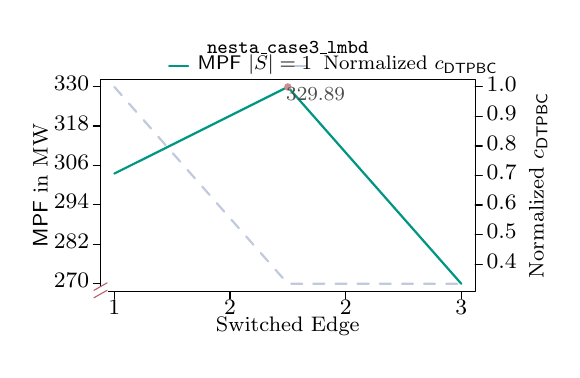
\begin{tikzpicture}[x=1pt,y=1pt]
\definecolor{fillColor}{RGB}{255,255,255}
\path[use as bounding box,fill=fillColor,fill opacity=0.00] (0,0) rectangle (440.85,271.01);
\begin{scope}
\path[clip] (  0.00,  0.00) rectangle (440.85,271.01);
\definecolor{drawColor}{RGB}{193,202,220}

\path[draw=drawColor,line width= 0.8pt,dash pattern=on 4pt off 4pt ,line join=round,line cap=round] ( 72.86,221.20) --
	(218.62, 55.82) --
	(364.39, 55.82);
\end{scope}
\begin{scope}
\path[clip] (  0.00,  0.00) rectangle (440.85,271.01);
\definecolor{drawColor}{RGB}{0,0,0}

\path[draw=drawColor,line width= 0.4pt,line join=round,line cap=round] ( 61.20, 49.20) --
	(376.05, 49.20) --
	(376.05,227.81) --
	( 61.20,227.81) --
	( 61.20, 49.20);
\end{scope}
\begin{scope}
\path[clip] (  0.00,  0.00) rectangle (440.85,271.01);
\definecolor{drawColor}{RGB}{0,0,0}

\path[draw=drawColor,line width= 0.4pt,line join=round,line cap=round] (376.05, 72.35) -- (376.05,221.20);

\path[draw=drawColor,line width= 0.4pt,line join=round,line cap=round] (376.05, 72.35) -- (382.05, 72.35);

\path[draw=drawColor,line width= 0.4pt,line join=round,line cap=round] (376.05, 97.16) -- (382.05, 97.16);

\path[draw=drawColor,line width= 0.4pt,line join=round,line cap=round] (376.05,121.97) -- (382.05,121.97);

\path[draw=drawColor,line width= 0.4pt,line join=round,line cap=round] (376.05,146.78) -- (382.05,146.78);

\path[draw=drawColor,line width= 0.4pt,line join=round,line cap=round] (376.05,171.58) -- (382.05,171.58);

\path[draw=drawColor,line width= 0.4pt,line join=round,line cap=round] (376.05,196.39) -- (382.05,196.39);

\path[draw=drawColor,line width= 0.4pt,line join=round,line cap=round] (376.05,221.20) -- (382.05,221.20);

\node[text=drawColor,anchor=base west,inner sep=0pt, outer sep=0pt, scale=  1.00] at (385.65, 68.91) {0.4};

\node[text=drawColor,anchor=base west,inner sep=0pt, outer sep=0pt, scale=  1.00] at (385.65, 93.72) {0.5};

\node[text=drawColor,anchor=base west,inner sep=0pt, outer sep=0pt, scale=  1.00] at (385.65,118.52) {0.6};

\node[text=drawColor,anchor=base west,inner sep=0pt, outer sep=0pt, scale=  1.00] at (385.65,143.33) {0.7};

\node[text=drawColor,anchor=base west,inner sep=0pt, outer sep=0pt, scale=  1.00] at (385.65,168.14) {0.8};

\node[text=drawColor,anchor=base west,inner sep=0pt, outer sep=0pt, scale=  1.00] at (385.65,192.95) {0.9};

\node[text=drawColor,anchor=base west,inner sep=0pt, outer sep=0pt, scale=  1.00] at (385.65,217.75) {1.0};
\end{scope}
\begin{scope}
\path[clip] (  0.00,  0.00) rectangle (440.85,271.01);
\definecolor{drawColor}{RGB}{0,150,130}

\path[draw=drawColor,line width= 0.8pt,line join=round,line cap=round] (118.89,238.60) -- (134.91,238.60);
\definecolor{drawColor}{RGB}{193,202,220}

\path[draw=drawColor,line width= 0.8pt,dash pattern=on 4pt off 4pt ,line join=round,line cap=round] (224.63,238.60) -- (240.65,238.60);
\definecolor{drawColor}{RGB}{0,0,0}

\node[text=drawColor,anchor=base,inner sep=0pt, outer sep=0pt, scale=  0.89] at (218.62,249.28) {\texttt{nesta\_case3\_lmbd}};

\node[text=drawColor,anchor=base west,inner sep=0pt, outer sep=0pt, scale=  0.89] at (142.92,235.54) {$\mathsf{MPF}~|S|=1$};

\node[text=drawColor,anchor=base west,inner sep=0pt, outer sep=0pt, scale=  0.89] at (248.66,235.54) {Normalized~$c_\mathsf{DTPBC}$};
\end{scope}
\begin{scope}
\path[clip] (  0.00,  0.00) rectangle (440.85,271.01);
\definecolor{drawColor}{RGB}{0,0,0}

\path[draw=drawColor,line width= 0.4pt,line join=round,line cap=round] ( 61.20, 55.82) -- ( 61.20,221.49);

\path[draw=drawColor,line width= 0.4pt,line join=round,line cap=round] ( 61.20, 55.82) -- ( 55.20, 55.82);

\path[draw=drawColor,line width= 0.4pt,line join=round,line cap=round] ( 61.20, 88.95) -- ( 55.20, 88.95);

\path[draw=drawColor,line width= 0.4pt,line join=round,line cap=round] ( 61.20,122.09) -- ( 55.20,122.09);

\path[draw=drawColor,line width= 0.4pt,line join=round,line cap=round] ( 61.20,155.22) -- ( 55.20,155.22);

\path[draw=drawColor,line width= 0.4pt,line join=round,line cap=round] ( 61.20,188.36) -- ( 55.20,188.36);

\path[draw=drawColor,line width= 0.4pt,line join=round,line cap=round] ( 61.20,221.49) -- ( 55.20,221.49);

\node[text=drawColor,anchor=base east,inner sep=0pt, outer sep=0pt, scale=  1.00] at ( 51.60, 52.37) {270};

\node[text=drawColor,anchor=base east,inner sep=0pt, outer sep=0pt, scale=  1.00] at ( 51.60, 85.51) {282};

\node[text=drawColor,anchor=base east,inner sep=0pt, outer sep=0pt, scale=  1.00] at ( 51.60,118.64) {294};

\node[text=drawColor,anchor=base east,inner sep=0pt, outer sep=0pt, scale=  1.00] at ( 51.60,151.78) {306};

\node[text=drawColor,anchor=base east,inner sep=0pt, outer sep=0pt, scale=  1.00] at ( 51.60,184.91) {318};

\node[text=drawColor,anchor=base east,inner sep=0pt, outer sep=0pt, scale=  1.00] at ( 51.60,218.05) {330};
\end{scope}
\begin{scope}
\path[clip] (  0.00,  0.00) rectangle (440.85,271.01);
\definecolor{drawColor}{RGB}{255,255,255}
\definecolor{fillColor}{RGB}{255,255,255}

\path[draw=drawColor,line width= 0.4pt,line join=round,line cap=round,fill=fillColor] ( 55.69, 47.17) rectangle ( 66.71, 53.42);
\definecolor{drawColor}{RGB}{188,97,104}

\path[draw=drawColor,line width= 0.4pt,line join=round,line cap=round] ( 55.69, 44.04) -- ( 66.71, 50.29);

\path[draw=drawColor,line width= 0.4pt,line join=round,line cap=round] ( 55.69, 50.29) -- ( 66.71, 56.54);
\end{scope}
\begin{scope}
\path[clip] ( 61.20, 49.20) rectangle (376.05,227.81);
\definecolor{drawColor}{RGB}{0,150,130}

\path[draw=drawColor,line width= 0.8pt,line join=round,line cap=round] ( 72.86,148.41) --
	(218.62,221.20) --
	(364.39, 55.82);
\end{scope}
\begin{scope}
\path[clip] ( 61.20, 49.20) rectangle (376.05,227.81);
\definecolor{fillColor}{RGB}{207,142,147}

\path[fill=fillColor] (218.62,221.20) circle (  3.15);
\end{scope}
\begin{scope}
\path[clip] ( 61.20, 49.20) rectangle (376.05,227.81);
\definecolor{drawColor}{gray}{0.30}

\node[text=drawColor,anchor=base,inner sep=0pt, outer sep=0pt, scale=  0.90] at (241.95,210.04) {329.89};
\end{scope}
\begin{scope}
\path[clip] (  0.00,  0.00) rectangle (440.85,271.01);
\definecolor{drawColor}{RGB}{0,0,0}

\path[draw=drawColor,line width= 0.4pt,line join=round,line cap=round] ( 72.86, 49.20) -- (364.39, 49.20);

\path[draw=drawColor,line width= 0.4pt,line join=round,line cap=round] ( 72.86, 49.20) -- ( 72.86, 43.20);

\path[draw=drawColor,line width= 0.4pt,line join=round,line cap=round] (170.04, 49.20) -- (170.04, 43.20);

\path[draw=drawColor,line width= 0.4pt,line join=round,line cap=round] (267.21, 49.20) -- (267.21, 43.20);

\path[draw=drawColor,line width= 0.4pt,line join=round,line cap=round] (364.39, 49.20) -- (364.39, 43.20);

\node[text=drawColor,anchor=base,inner sep=0pt, outer sep=0pt, scale=  1.00] at ( 72.86, 30.00) {1};

\node[text=drawColor,anchor=base,inner sep=0pt, outer sep=0pt, scale=  1.00] at (170.04, 30.00) {2};

\node[text=drawColor,anchor=base,inner sep=0pt, outer sep=0pt, scale=  1.00] at (267.21, 30.00) {2};

\node[text=drawColor,anchor=base,inner sep=0pt, outer sep=0pt, scale=  1.00] at (364.39, 30.00) {3};

\node[text=drawColor,anchor=base,inner sep=0pt, outer sep=0pt, scale=  0.95] at (218.62, 15.60) {Switched Edge};

\node[text=drawColor,rotate= 90.00,anchor=base,inner sep=0pt, outer sep=0pt, scale=  0.95] at ( 16.80,138.51) {$\mathsf{MPF}$ in~$\mathrm{MW}$};

\node[text=drawColor,rotate= 90.00,anchor=base,inner sep=0pt, outer sep=0pt, scale=  0.95] at (433.65,138.51) {Normalized~$c_\mathsf{DTPBC}$};
\end{scope}
\end{tikzpicture}
%
    \label{fig:SwitchingBetweenness_nesta_case3_lmbd_dtpbc_mpf_cutY}%
  \end{subfigure}%
  \hfill%
  \begin{subfigure}[t]{.5\textwidth}%
    \centering%
    \input{switchplacement/plots/plot-SwitchingBetweenness_nesta_case4_gs-dtpbc-mpf-cutY.tex}%
    \label{plot:SwitchingBetweenness_nesta_case4_gs_dtpbc_mpf_cutY}%
  \end{subfigure}%

  \begin{subfigure}[t]{.5\textwidth}%
    \centering%
    % Created by tikzDevice version 0.10.1 on 2018-01-31 10:28:32
% !TEX encoding = UTF-8 Unicode
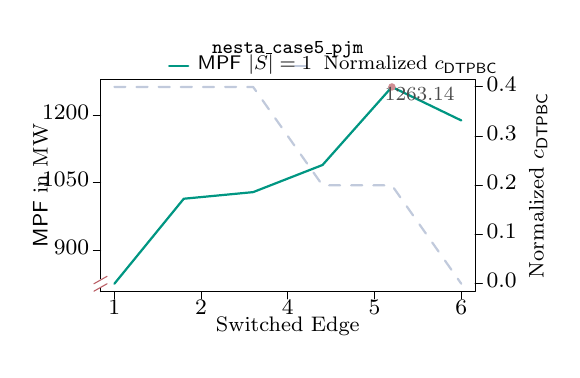
\begin{tikzpicture}[x=1pt,y=1pt]
\definecolor{fillColor}{RGB}{255,255,255}
\path[use as bounding box,fill=fillColor,fill opacity=0.00] (0,0) rectangle (440.85,271.01);
\begin{scope}
\path[clip] (  0.00,  0.00) rectangle (440.85,271.01);
\definecolor{drawColor}{RGB}{193,202,220}

\path[draw=drawColor,line width= 0.8pt,dash pattern=on 4pt off 4pt ,line join=round,line cap=round] ( 72.86,221.20) --
	(131.17,221.20) --
	(189.47,221.20) --
	(247.78,138.51) --
	(306.08,138.51) --
	(364.39, 55.82);
\end{scope}
\begin{scope}
\path[clip] (  0.00,  0.00) rectangle (440.85,271.01);
\definecolor{drawColor}{RGB}{0,0,0}

\path[draw=drawColor,line width= 0.4pt,line join=round,line cap=round] ( 61.20, 49.20) --
	(376.05, 49.20) --
	(376.05,227.81) --
	( 61.20,227.81) --
	( 61.20, 49.20);
\end{scope}
\begin{scope}
\path[clip] (  0.00,  0.00) rectangle (440.85,271.01);
\definecolor{drawColor}{RGB}{0,0,0}

\path[draw=drawColor,line width= 0.4pt,line join=round,line cap=round] (376.05, 55.82) -- (376.05,221.20);

\path[draw=drawColor,line width= 0.4pt,line join=round,line cap=round] (376.05, 55.82) -- (382.05, 55.82);

\path[draw=drawColor,line width= 0.4pt,line join=round,line cap=round] (376.05, 97.16) -- (382.05, 97.16);

\path[draw=drawColor,line width= 0.4pt,line join=round,line cap=round] (376.05,138.51) -- (382.05,138.51);

\path[draw=drawColor,line width= 0.4pt,line join=round,line cap=round] (376.05,179.85) -- (382.05,179.85);

\path[draw=drawColor,line width= 0.4pt,line join=round,line cap=round] (376.05,221.20) -- (382.05,221.20);

\node[text=drawColor,anchor=base west,inner sep=0pt, outer sep=0pt, scale=  1.00] at (385.65, 52.37) {0.0};

\node[text=drawColor,anchor=base west,inner sep=0pt, outer sep=0pt, scale=  1.00] at (385.65, 93.72) {0.1};

\node[text=drawColor,anchor=base west,inner sep=0pt, outer sep=0pt, scale=  1.00] at (385.65,135.06) {0.2};

\node[text=drawColor,anchor=base west,inner sep=0pt, outer sep=0pt, scale=  1.00] at (385.65,176.41) {0.3};

\node[text=drawColor,anchor=base west,inner sep=0pt, outer sep=0pt, scale=  1.00] at (385.65,217.75) {0.4};
\end{scope}
\begin{scope}
\path[clip] (  0.00,  0.00) rectangle (440.85,271.01);
\definecolor{drawColor}{RGB}{0,150,130}

\path[draw=drawColor,line width= 0.8pt,line join=round,line cap=round] (118.89,238.60) -- (134.91,238.60);
\definecolor{drawColor}{RGB}{193,202,220}

\path[draw=drawColor,line width= 0.8pt,dash pattern=on 4pt off 4pt ,line join=round,line cap=round] (224.63,238.60) -- (240.65,238.60);
\definecolor{drawColor}{RGB}{0,0,0}

\node[text=drawColor,anchor=base,inner sep=0pt, outer sep=0pt, scale=  0.89] at (218.62,249.28) {\texttt{nesta\_case5\_pjm}};

\node[text=drawColor,anchor=base west,inner sep=0pt, outer sep=0pt, scale=  0.89] at (142.92,235.54) {$\mathsf{MPF}~|S|=1$};

\node[text=drawColor,anchor=base west,inner sep=0pt, outer sep=0pt, scale=  0.89] at (248.66,235.54) {Normalized~$c_\mathsf{DTPBC}$};
\end{scope}
\begin{scope}
\path[clip] (  0.00,  0.00) rectangle (440.85,271.01);
\definecolor{drawColor}{RGB}{0,0,0}

\path[draw=drawColor,line width= 0.4pt,line join=round,line cap=round] ( 61.20, 83.86) -- ( 61.20,197.32);

\path[draw=drawColor,line width= 0.4pt,line join=round,line cap=round] ( 61.20, 83.86) -- ( 55.20, 83.86);

\path[draw=drawColor,line width= 0.4pt,line join=round,line cap=round] ( 61.20,140.59) -- ( 55.20,140.59);

\path[draw=drawColor,line width= 0.4pt,line join=round,line cap=round] ( 61.20,197.32) -- ( 55.20,197.32);

\node[text=drawColor,anchor=base east,inner sep=0pt, outer sep=0pt, scale=  1.00] at ( 51.60, 80.42) {900};

\node[text=drawColor,anchor=base east,inner sep=0pt, outer sep=0pt, scale=  1.00] at ( 51.60,137.14) {1050};

\node[text=drawColor,anchor=base east,inner sep=0pt, outer sep=0pt, scale=  1.00] at ( 51.60,193.87) {1200};
\end{scope}
\begin{scope}
\path[clip] (  0.00,  0.00) rectangle (440.85,271.01);
\definecolor{drawColor}{RGB}{255,255,255}
\definecolor{fillColor}{RGB}{255,255,255}

\path[draw=drawColor,line width= 0.4pt,line join=round,line cap=round,fill=fillColor] ( 55.69, 52.69) rectangle ( 66.71, 58.94);
\definecolor{drawColor}{RGB}{188,97,104}

\path[draw=drawColor,line width= 0.4pt,line join=round,line cap=round] ( 55.69, 49.56) -- ( 66.71, 55.82);

\path[draw=drawColor,line width= 0.4pt,line join=round,line cap=round] ( 55.69, 55.82) -- ( 66.71, 62.07);
\end{scope}
\begin{scope}
\path[clip] ( 61.20, 49.20) rectangle (376.05,227.81);
\definecolor{drawColor}{RGB}{0,150,130}

\path[draw=drawColor,line width= 0.8pt,line join=round,line cap=round] ( 72.86, 55.82) --
	(131.17,127.25) --
	(189.47,132.81) --
	(247.78,155.61) --
	(306.08,221.20) --
	(364.39,193.03);
\end{scope}
\begin{scope}
\path[clip] ( 61.20, 49.20) rectangle (376.05,227.81);
\definecolor{fillColor}{RGB}{207,142,147}

\path[fill=fillColor] (306.08,221.20) circle (  3.15);
\end{scope}
\begin{scope}
\path[clip] ( 61.20, 49.20) rectangle (376.05,227.81);
\definecolor{drawColor}{gray}{0.30}

\node[text=drawColor,anchor=base,inner sep=0pt, outer sep=0pt, scale=  0.90] at (329.40,210.04) {1263.14};
\end{scope}
\begin{scope}
\path[clip] (  0.00,  0.00) rectangle (440.85,271.01);
\definecolor{drawColor}{RGB}{0,0,0}

\path[draw=drawColor,line width= 0.4pt,line join=round,line cap=round] ( 72.86, 49.20) -- (364.39, 49.20);

\path[draw=drawColor,line width= 0.4pt,line join=round,line cap=round] ( 72.86, 49.20) -- ( 72.86, 43.20);

\path[draw=drawColor,line width= 0.4pt,line join=round,line cap=round] (145.74, 49.20) -- (145.74, 43.20);

\path[draw=drawColor,line width= 0.4pt,line join=round,line cap=round] (218.62, 49.20) -- (218.62, 43.20);

\path[draw=drawColor,line width= 0.4pt,line join=round,line cap=round] (291.50, 49.20) -- (291.50, 43.20);

\path[draw=drawColor,line width= 0.4pt,line join=round,line cap=round] (364.39, 49.20) -- (364.39, 43.20);

\node[text=drawColor,anchor=base,inner sep=0pt, outer sep=0pt, scale=  1.00] at ( 72.86, 30.00) {1};

\node[text=drawColor,anchor=base,inner sep=0pt, outer sep=0pt, scale=  1.00] at (145.74, 30.00) {2};

\node[text=drawColor,anchor=base,inner sep=0pt, outer sep=0pt, scale=  1.00] at (218.62, 30.00) {4};

\node[text=drawColor,anchor=base,inner sep=0pt, outer sep=0pt, scale=  1.00] at (291.50, 30.00) {5};

\node[text=drawColor,anchor=base,inner sep=0pt, outer sep=0pt, scale=  1.00] at (364.39, 30.00) {6};

\node[text=drawColor,anchor=base,inner sep=0pt, outer sep=0pt, scale=  0.95] at (218.62, 15.60) {Switched Edge};

\node[text=drawColor,rotate= 90.00,anchor=base,inner sep=0pt, outer sep=0pt, scale=  0.95] at ( 16.80,138.51) {$\mathsf{MPF}$ in~$\mathrm{MW}$};

\node[text=drawColor,rotate= 90.00,anchor=base,inner sep=0pt, outer sep=0pt, scale=  0.95] at (433.65,138.51) {Normalized~$c_\mathsf{DTPBC}$};
\end{scope}
\end{tikzpicture}
%
    \label{plot:SwitchingBetweenness_nesta_case5_pjm_dtpbc_mpf_cutY}%
  \end{subfigure}%
  \hfill%
  \begin{subfigure}[t]{.5\textwidth}%
    \centering%
    % Created by tikzDevice version 0.10.1 on 2018-01-31 10:28:39
% !TEX encoding = UTF-8 Unicode
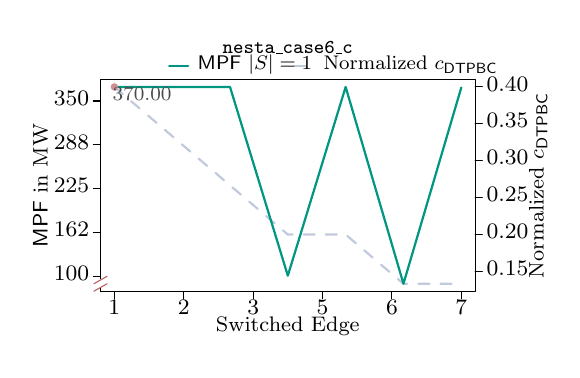
\begin{tikzpicture}[x=1pt,y=1pt]
\definecolor{fillColor}{RGB}{255,255,255}
\path[use as bounding box,fill=fillColor,fill opacity=0.00] (0,0) rectangle (440.85,271.01);
\begin{scope}
\path[clip] (  0.00,  0.00) rectangle (440.85,271.01);
\definecolor{drawColor}{RGB}{193,202,220}

\path[draw=drawColor,line width= 0.8pt,dash pattern=on 4pt off 4pt ,line join=round,line cap=round] ( 72.86,221.20) --
	(121.45,179.85) --
	(170.04,138.51) --
	(218.62, 97.16) --
	(267.21, 97.16) --
	(315.80, 55.82) --
	(364.39, 55.82);
\end{scope}
\begin{scope}
\path[clip] (  0.00,  0.00) rectangle (440.85,271.01);
\definecolor{drawColor}{RGB}{0,0,0}

\path[draw=drawColor,line width= 0.4pt,line join=round,line cap=round] ( 61.20, 49.20) --
	(376.05, 49.20) --
	(376.05,227.81) --
	( 61.20,227.81) --
	( 61.20, 49.20);
\end{scope}
\begin{scope}
\path[clip] (  0.00,  0.00) rectangle (440.85,271.01);
\definecolor{drawColor}{RGB}{0,0,0}

\path[draw=drawColor,line width= 0.4pt,line join=round,line cap=round] (376.05, 66.15) -- (376.05,221.20);

\path[draw=drawColor,line width= 0.4pt,line join=round,line cap=round] (376.05, 66.15) -- (382.05, 66.15);

\path[draw=drawColor,line width= 0.4pt,line join=round,line cap=round] (376.05, 97.16) -- (382.05, 97.16);

\path[draw=drawColor,line width= 0.4pt,line join=round,line cap=round] (376.05,128.17) -- (382.05,128.17);

\path[draw=drawColor,line width= 0.4pt,line join=round,line cap=round] (376.05,159.18) -- (382.05,159.18);

\path[draw=drawColor,line width= 0.4pt,line join=round,line cap=round] (376.05,190.19) -- (382.05,190.19);

\path[draw=drawColor,line width= 0.4pt,line join=round,line cap=round] (376.05,221.20) -- (382.05,221.20);

\node[text=drawColor,anchor=base west,inner sep=0pt, outer sep=0pt, scale=  1.00] at (385.65, 62.71) {0.15};

\node[text=drawColor,anchor=base west,inner sep=0pt, outer sep=0pt, scale=  1.00] at (385.65, 93.72) {0.20};

\node[text=drawColor,anchor=base west,inner sep=0pt, outer sep=0pt, scale=  1.00] at (385.65,124.73) {0.25};

\node[text=drawColor,anchor=base west,inner sep=0pt, outer sep=0pt, scale=  1.00] at (385.65,155.74) {0.30};

\node[text=drawColor,anchor=base west,inner sep=0pt, outer sep=0pt, scale=  1.00] at (385.65,186.74) {0.35};

\node[text=drawColor,anchor=base west,inner sep=0pt, outer sep=0pt, scale=  1.00] at (385.65,217.75) {0.40};
\end{scope}
\begin{scope}
\path[clip] (  0.00,  0.00) rectangle (440.85,271.01);
\definecolor{drawColor}{RGB}{0,150,130}

\path[draw=drawColor,line width= 0.8pt,line join=round,line cap=round] (118.89,238.60) -- (134.91,238.60);
\definecolor{drawColor}{RGB}{193,202,220}

\path[draw=drawColor,line width= 0.8pt,dash pattern=on 4pt off 4pt ,line join=round,line cap=round] (224.63,238.60) -- (240.65,238.60);
\definecolor{drawColor}{RGB}{0,0,0}

\node[text=drawColor,anchor=base,inner sep=0pt, outer sep=0pt, scale=  0.89] at (218.62,249.28) {\texttt{nesta\_case6\_c}};

\node[text=drawColor,anchor=base west,inner sep=0pt, outer sep=0pt, scale=  0.89] at (142.92,235.54) {$\mathsf{MPF}~|S|=1$};

\node[text=drawColor,anchor=base west,inner sep=0pt, outer sep=0pt, scale=  0.89] at (248.66,235.54) {Normalized~$c_\mathsf{DTPBC}$};
\end{scope}
\begin{scope}
\path[clip] (  0.00,  0.00) rectangle (440.85,271.01);
\definecolor{drawColor}{RGB}{0,0,0}

\path[draw=drawColor,line width= 0.4pt,line join=round,line cap=round] ( 61.20, 61.79) -- ( 61.20,209.39);

\path[draw=drawColor,line width= 0.4pt,line join=round,line cap=round] ( 61.20, 61.79) -- ( 55.20, 61.79);

\path[draw=drawColor,line width= 0.4pt,line join=round,line cap=round] ( 61.20, 98.69) -- ( 55.20, 98.69);

\path[draw=drawColor,line width= 0.4pt,line join=round,line cap=round] ( 61.20,135.59) -- ( 55.20,135.59);

\path[draw=drawColor,line width= 0.4pt,line join=round,line cap=round] ( 61.20,172.49) -- ( 55.20,172.49);

\path[draw=drawColor,line width= 0.4pt,line join=round,line cap=round] ( 61.20,209.39) -- ( 55.20,209.39);

\node[text=drawColor,anchor=base east,inner sep=0pt, outer sep=0pt, scale=  1.00] at ( 51.60, 58.34) {100};

\node[text=drawColor,anchor=base east,inner sep=0pt, outer sep=0pt, scale=  1.00] at ( 51.60, 95.24) {162};

\node[text=drawColor,anchor=base east,inner sep=0pt, outer sep=0pt, scale=  1.00] at ( 51.60,132.14) {225};

\node[text=drawColor,anchor=base east,inner sep=0pt, outer sep=0pt, scale=  1.00] at ( 51.60,169.04) {288};

\node[text=drawColor,anchor=base east,inner sep=0pt, outer sep=0pt, scale=  1.00] at ( 51.60,205.95) {350};
\end{scope}
\begin{scope}
\path[clip] (  0.00,  0.00) rectangle (440.85,271.01);
\definecolor{drawColor}{RGB}{255,255,255}
\definecolor{fillColor}{RGB}{255,255,255}

\path[draw=drawColor,line width= 0.4pt,line join=round,line cap=round,fill=fillColor] ( 55.69, 52.69) rectangle ( 66.71, 58.94);
\definecolor{drawColor}{RGB}{188,97,104}

\path[draw=drawColor,line width= 0.4pt,line join=round,line cap=round] ( 55.69, 49.56) -- ( 66.71, 55.82);

\path[draw=drawColor,line width= 0.4pt,line join=round,line cap=round] ( 55.69, 55.82) -- ( 66.71, 62.07);
\end{scope}
\begin{scope}
\path[clip] ( 61.20, 49.20) rectangle (376.05,227.81);
\definecolor{drawColor}{RGB}{0,150,130}

\path[draw=drawColor,line width= 0.8pt,line join=round,line cap=round] ( 72.86,221.20) --
	(121.45,221.20) --
	(170.04,221.20) --
	(218.62, 62.60) --
	(267.21,221.20) --
	(315.80, 55.82) --
	(364.39,220.67);
\end{scope}
\begin{scope}
\path[clip] ( 61.20, 49.20) rectangle (376.05,227.81);
\definecolor{fillColor}{RGB}{207,142,147}

\path[fill=fillColor] ( 72.86,221.20) circle (  3.15);
\end{scope}
\begin{scope}
\path[clip] ( 61.20, 49.20) rectangle (376.05,227.81);
\definecolor{drawColor}{gray}{0.30}

\node[text=drawColor,anchor=base,inner sep=0pt, outer sep=0pt, scale=  0.90] at ( 96.18,210.04) {370.00};
\end{scope}
\begin{scope}
\path[clip] (  0.00,  0.00) rectangle (440.85,271.01);
\definecolor{drawColor}{RGB}{0,0,0}

\path[draw=drawColor,line width= 0.4pt,line join=round,line cap=round] ( 72.86, 49.20) -- (364.39, 49.20);

\path[draw=drawColor,line width= 0.4pt,line join=round,line cap=round] ( 72.86, 49.20) -- ( 72.86, 43.20);

\path[draw=drawColor,line width= 0.4pt,line join=round,line cap=round] (131.17, 49.20) -- (131.17, 43.20);

\path[draw=drawColor,line width= 0.4pt,line join=round,line cap=round] (189.47, 49.20) -- (189.47, 43.20);

\path[draw=drawColor,line width= 0.4pt,line join=round,line cap=round] (247.78, 49.20) -- (247.78, 43.20);

\path[draw=drawColor,line width= 0.4pt,line join=round,line cap=round] (306.08, 49.20) -- (306.08, 43.20);

\path[draw=drawColor,line width= 0.4pt,line join=round,line cap=round] (364.39, 49.20) -- (364.39, 43.20);

\node[text=drawColor,anchor=base,inner sep=0pt, outer sep=0pt, scale=  1.00] at ( 72.86, 30.00) {1};

\node[text=drawColor,anchor=base,inner sep=0pt, outer sep=0pt, scale=  1.00] at (131.17, 30.00) {2};

\node[text=drawColor,anchor=base,inner sep=0pt, outer sep=0pt, scale=  1.00] at (189.47, 30.00) {3};

\node[text=drawColor,anchor=base,inner sep=0pt, outer sep=0pt, scale=  1.00] at (247.78, 30.00) {5};

\node[text=drawColor,anchor=base,inner sep=0pt, outer sep=0pt, scale=  1.00] at (306.08, 30.00) {6};

\node[text=drawColor,anchor=base,inner sep=0pt, outer sep=0pt, scale=  1.00] at (364.39, 30.00) {7};

\node[text=drawColor,anchor=base,inner sep=0pt, outer sep=0pt, scale=  0.95] at (218.62, 15.60) {Switched Edge};

\node[text=drawColor,rotate= 90.00,anchor=base,inner sep=0pt, outer sep=0pt, scale=  0.95] at ( 16.80,138.51) {$\mathsf{MPF}$ in~$\mathrm{MW}$};

\node[text=drawColor,rotate= 90.00,anchor=base,inner sep=0pt, outer sep=0pt, scale=  0.95] at (433.65,138.51) {Normalized~$c_\mathsf{DTPBC}$};
\end{scope}
\end{tikzpicture}
%
    \label{plot:SwitchingBetweenness_nesta_case6_c_dtpbc_mpf_cutY}%
  \end{subfigure}%

  \begin{subfigure}[t]{.5\textwidth}%
    \centering%
    % Created by tikzDevice version 0.10.1 on 2018-01-31 10:28:43
% !TEX encoding = UTF-8 Unicode
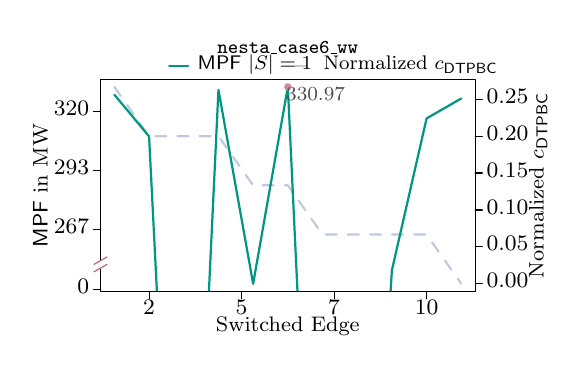
\begin{tikzpicture}[x=1pt,y=1pt]
\definecolor{fillColor}{RGB}{255,255,255}
\path[use as bounding box,fill=fillColor,fill opacity=0.00] (0,0) rectangle (440.85,271.01);
\begin{scope}
\path[clip] (  0.00,  0.00) rectangle (440.85,271.01);
\definecolor{drawColor}{RGB}{193,202,220}

\path[draw=drawColor,line width= 0.8pt,dash pattern=on 4pt off 4pt ,line join=round,line cap=round] ( 72.86,221.20) --
	(102.01,179.85) --
	(131.17,179.85) --
	(160.32,179.85) --
	(189.47,138.51) --
	(218.62,138.51) --
	(247.78, 97.16) --
	(276.93, 97.16) --
	(306.08, 97.16) --
	(335.23, 97.16) --
	(364.39, 55.82);
\end{scope}
\begin{scope}
\path[clip] (  0.00,  0.00) rectangle (440.85,271.01);
\definecolor{drawColor}{RGB}{0,0,0}

\path[draw=drawColor,line width= 0.4pt,line join=round,line cap=round] ( 61.20, 49.20) --
	(376.05, 49.20) --
	(376.05,227.81) --
	( 61.20,227.81) --
	( 61.20, 49.20);
\end{scope}
\begin{scope}
\path[clip] (  0.00,  0.00) rectangle (440.85,271.01);
\definecolor{drawColor}{RGB}{0,0,0}

\path[draw=drawColor,line width= 0.4pt,line join=round,line cap=round] (376.05, 55.82) -- (376.05,210.86);

\path[draw=drawColor,line width= 0.4pt,line join=round,line cap=round] (376.05, 55.82) -- (382.05, 55.82);

\path[draw=drawColor,line width= 0.4pt,line join=round,line cap=round] (376.05, 86.82) -- (382.05, 86.82);

\path[draw=drawColor,line width= 0.4pt,line join=round,line cap=round] (376.05,117.83) -- (382.05,117.83);

\path[draw=drawColor,line width= 0.4pt,line join=round,line cap=round] (376.05,148.84) -- (382.05,148.84);

\path[draw=drawColor,line width= 0.4pt,line join=round,line cap=round] (376.05,179.85) -- (382.05,179.85);

\path[draw=drawColor,line width= 0.4pt,line join=round,line cap=round] (376.05,210.86) -- (382.05,210.86);

\node[text=drawColor,anchor=base west,inner sep=0pt, outer sep=0pt, scale=  1.00] at (385.65, 52.37) {0.00};

\node[text=drawColor,anchor=base west,inner sep=0pt, outer sep=0pt, scale=  1.00] at (385.65, 83.38) {0.05};

\node[text=drawColor,anchor=base west,inner sep=0pt, outer sep=0pt, scale=  1.00] at (385.65,114.39) {0.10};

\node[text=drawColor,anchor=base west,inner sep=0pt, outer sep=0pt, scale=  1.00] at (385.65,145.40) {0.15};

\node[text=drawColor,anchor=base west,inner sep=0pt, outer sep=0pt, scale=  1.00] at (385.65,176.41) {0.20};

\node[text=drawColor,anchor=base west,inner sep=0pt, outer sep=0pt, scale=  1.00] at (385.65,207.42) {0.25};
\end{scope}
\begin{scope}
\path[clip] (  0.00,  0.00) rectangle (440.85,271.01);
\definecolor{drawColor}{RGB}{0,150,130}

\path[draw=drawColor,line width= 0.8pt,line join=round,line cap=round] (118.89,238.60) -- (134.91,238.60);
\definecolor{drawColor}{RGB}{193,202,220}

\path[draw=drawColor,line width= 0.8pt,dash pattern=on 4pt off 4pt ,line join=round,line cap=round] (224.63,238.60) -- (240.65,238.60);
\definecolor{drawColor}{RGB}{0,0,0}

\node[text=drawColor,anchor=base,inner sep=0pt, outer sep=0pt, scale=  0.89] at (218.62,249.28) {\texttt{nesta\_case6\_ww}};

\node[text=drawColor,anchor=base west,inner sep=0pt, outer sep=0pt, scale=  0.89] at (142.92,235.54) {$\mathsf{MPF}~|S|=1$};

\node[text=drawColor,anchor=base west,inner sep=0pt, outer sep=0pt, scale=  0.89] at (248.66,235.54) {Normalized~$c_\mathsf{DTPBC}$};
\end{scope}
\begin{scope}
\path[clip] (  0.00,  0.00) rectangle (440.85,271.01);
\definecolor{drawColor}{RGB}{0,0,0}

\path[draw=drawColor,line width= 0.4pt,line join=round,line cap=round] ( 61.20, 51.35) -- ( 61.20,200.71);

\path[draw=drawColor,line width= 0.4pt,line join=round,line cap=round] ( 61.20, 51.35) -- ( 55.20, 51.35);

\path[draw=drawColor,line width= 0.4pt,line join=round,line cap=round] ( 61.20,101.13) -- ( 55.20,101.13);

\path[draw=drawColor,line width= 0.4pt,line join=round,line cap=round] ( 61.20,150.92) -- ( 55.20,150.92);

\path[draw=drawColor,line width= 0.4pt,line join=round,line cap=round] ( 61.20,200.71) -- ( 55.20,200.71);

\node[text=drawColor,anchor=base east,inner sep=0pt, outer sep=0pt, scale=  1.00] at ( 51.60, 47.90) {0};

\node[text=drawColor,anchor=base east,inner sep=0pt, outer sep=0pt, scale=  1.00] at ( 51.60, 97.69) {267};

\node[text=drawColor,anchor=base east,inner sep=0pt, outer sep=0pt, scale=  1.00] at ( 51.60,147.48) {293};

\node[text=drawColor,anchor=base east,inner sep=0pt, outer sep=0pt, scale=  1.00] at ( 51.60,197.26) {320};
\end{scope}
\begin{scope}
\path[clip] (  0.00,  0.00) rectangle (440.85,271.01);
\definecolor{drawColor}{RGB}{255,255,255}
\definecolor{fillColor}{RGB}{255,255,255}

\path[draw=drawColor,line width= 0.4pt,line join=round,line cap=round,fill=fillColor] ( 55.69, 68.96) rectangle ( 66.71, 75.22);
\definecolor{drawColor}{RGB}{188,97,104}

\path[draw=drawColor,line width= 0.4pt,line join=round,line cap=round] ( 55.69, 65.84) -- ( 66.71, 72.09);

\path[draw=drawColor,line width= 0.4pt,line join=round,line cap=round] ( 55.69, 72.09) -- ( 66.71, 78.34);
\end{scope}
\begin{scope}
\path[clip] ( 61.20, 49.20) rectangle (376.05,227.81);
\definecolor{drawColor}{RGB}{0,150,130}

\path[draw=drawColor,line width= 0.8pt,line join=round,line cap=round] ( 72.86,214.69) --
	(102.01,179.67) --
	(111.10,  0.00);

\path[draw=drawColor,line width= 0.8pt,line join=round,line cap=round] (149.96,  0.00) --
	(160.32,218.72) --
	(189.47, 55.82) --
	(218.62,221.20) --
	(229.06,  0.00);

\path[draw=drawColor,line width= 0.8pt,line join=round,line cap=round] (301.86,  0.00) --
	(306.08, 67.19) --
	(335.23,194.75) --
	(364.39,211.52);
\end{scope}
\begin{scope}
\path[clip] ( 61.20, 49.20) rectangle (376.05,227.81);
\definecolor{fillColor}{RGB}{207,142,147}

\path[fill=fillColor] (218.62,221.20) circle (  3.15);
\end{scope}
\begin{scope}
\path[clip] ( 61.20, 49.20) rectangle (376.05,227.81);
\definecolor{drawColor}{gray}{0.30}

\node[text=drawColor,anchor=base,inner sep=0pt, outer sep=0pt, scale=  0.90] at (241.95,210.04) {330.97};
\end{scope}
\begin{scope}
\path[clip] (  0.00,  0.00) rectangle (440.85,271.01);
\definecolor{drawColor}{RGB}{0,0,0}

\path[draw=drawColor,line width= 0.4pt,line join=round,line cap=round] (102.01, 49.20) -- (335.23, 49.20);

\path[draw=drawColor,line width= 0.4pt,line join=round,line cap=round] (102.01, 49.20) -- (102.01, 43.20);

\path[draw=drawColor,line width= 0.4pt,line join=round,line cap=round] (179.75, 49.20) -- (179.75, 43.20);

\path[draw=drawColor,line width= 0.4pt,line join=round,line cap=round] (257.49, 49.20) -- (257.49, 43.20);

\path[draw=drawColor,line width= 0.4pt,line join=round,line cap=round] (335.23, 49.20) -- (335.23, 43.20);

\node[text=drawColor,anchor=base,inner sep=0pt, outer sep=0pt, scale=  1.00] at (102.01, 30.00) {2};

\node[text=drawColor,anchor=base,inner sep=0pt, outer sep=0pt, scale=  1.00] at (179.75, 30.00) {5};

\node[text=drawColor,anchor=base,inner sep=0pt, outer sep=0pt, scale=  1.00] at (257.49, 30.00) {7};

\node[text=drawColor,anchor=base,inner sep=0pt, outer sep=0pt, scale=  1.00] at (335.23, 30.00) {10};

\node[text=drawColor,anchor=base,inner sep=0pt, outer sep=0pt, scale=  0.95] at (218.62, 15.60) {Switched Edge};

\node[text=drawColor,rotate= 90.00,anchor=base,inner sep=0pt, outer sep=0pt, scale=  0.95] at ( 16.80,138.51) {$\mathsf{MPF}$ in~$\mathrm{MW}$};

\node[text=drawColor,rotate= 90.00,anchor=base,inner sep=0pt, outer sep=0pt, scale=  0.95] at (433.65,138.51) {Normalized~$c_\mathsf{DTPBC}$};
\end{scope}
\end{tikzpicture}
%
  \label{plot:SwitchingBetweenness_nesta_case6_ww_dtpbc_mpf_cutY}%
  \end{subfigure}%
  \hfill%
  \begin{subfigure}[t]{.5\textwidth}%
    \centering%
    % Created by tikzDevice version 0.10.1 on 2018-01-31 10:28:56
% !TEX encoding = UTF-8 Unicode
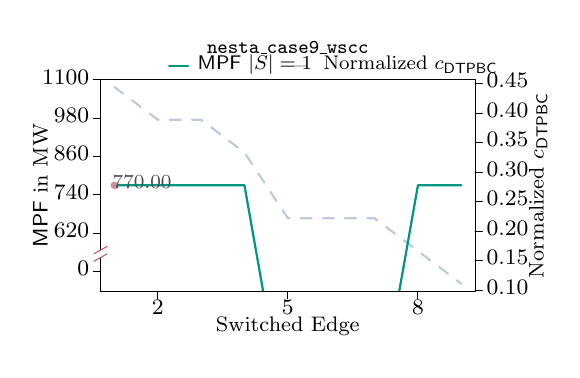
\begin{tikzpicture}[x=1pt,y=1pt]
\definecolor{fillColor}{RGB}{255,255,255}
\path[use as bounding box,fill=fillColor,fill opacity=0.00] (0,0) rectangle (440.85,271.01);
\begin{scope}
\path[clip] (  0.00,  0.00) rectangle (440.85,271.01);
\definecolor{drawColor}{RGB}{193,202,220}

\path[draw=drawColor,line width= 0.8pt,dash pattern=on 4pt off 4pt ,line join=round,line cap=round] ( 72.86,221.20) --
	(109.30,193.63) --
	(145.74,193.63) --
	(182.18,166.07) --
	(218.62,110.94) --
	(255.06,110.94) --
	(291.50,110.94) --
	(327.95, 83.38) --
	(364.39, 55.82);
\end{scope}
\begin{scope}
\path[clip] (  0.00,  0.00) rectangle (440.85,271.01);
\definecolor{drawColor}{RGB}{0,0,0}

\path[draw=drawColor,line width= 0.4pt,line join=round,line cap=round] ( 61.20, 49.20) --
	(376.05, 49.20) --
	(376.05,227.81) --
	( 61.20,227.81) --
	( 61.20, 49.20);
\end{scope}
\begin{scope}
\path[clip] (  0.00,  0.00) rectangle (440.85,271.01);
\definecolor{drawColor}{RGB}{0,0,0}

\path[draw=drawColor,line width= 0.4pt,line join=round,line cap=round] (376.05, 50.30) -- (376.05,223.95);

\path[draw=drawColor,line width= 0.4pt,line join=round,line cap=round] (376.05, 50.30) -- (382.05, 50.30);

\path[draw=drawColor,line width= 0.4pt,line join=round,line cap=round] (376.05, 75.11) -- (382.05, 75.11);

\path[draw=drawColor,line width= 0.4pt,line join=round,line cap=round] (376.05, 99.92) -- (382.05, 99.92);

\path[draw=drawColor,line width= 0.4pt,line join=round,line cap=round] (376.05,124.72) -- (382.05,124.72);

\path[draw=drawColor,line width= 0.4pt,line join=round,line cap=round] (376.05,149.53) -- (382.05,149.53);

\path[draw=drawColor,line width= 0.4pt,line join=round,line cap=round] (376.05,174.34) -- (382.05,174.34);

\path[draw=drawColor,line width= 0.4pt,line join=round,line cap=round] (376.05,199.15) -- (382.05,199.15);

\path[draw=drawColor,line width= 0.4pt,line join=round,line cap=round] (376.05,223.95) -- (382.05,223.95);

\node[text=drawColor,anchor=base west,inner sep=0pt, outer sep=0pt, scale=  1.00] at (385.65, 46.86) {0.10};

\node[text=drawColor,anchor=base west,inner sep=0pt, outer sep=0pt, scale=  1.00] at (385.65, 71.67) {0.15};

\node[text=drawColor,anchor=base west,inner sep=0pt, outer sep=0pt, scale=  1.00] at (385.65, 96.47) {0.20};

\node[text=drawColor,anchor=base west,inner sep=0pt, outer sep=0pt, scale=  1.00] at (385.65,121.28) {0.25};

\node[text=drawColor,anchor=base west,inner sep=0pt, outer sep=0pt, scale=  1.00] at (385.65,146.09) {0.30};

\node[text=drawColor,anchor=base west,inner sep=0pt, outer sep=0pt, scale=  1.00] at (385.65,170.90) {0.35};

\node[text=drawColor,anchor=base west,inner sep=0pt, outer sep=0pt, scale=  1.00] at (385.65,195.70) {0.40};

\node[text=drawColor,anchor=base west,inner sep=0pt, outer sep=0pt, scale=  1.00] at (385.65,220.51) {0.45};
\end{scope}
\begin{scope}
\path[clip] (  0.00,  0.00) rectangle (440.85,271.01);
\definecolor{drawColor}{RGB}{0,150,130}

\path[draw=drawColor,line width= 0.8pt,line join=round,line cap=round] (118.89,238.60) -- (134.91,238.60);
\definecolor{drawColor}{RGB}{193,202,220}

\path[draw=drawColor,line width= 0.8pt,dash pattern=on 4pt off 4pt ,line join=round,line cap=round] (224.63,238.60) -- (240.65,238.60);
\definecolor{drawColor}{RGB}{0,0,0}

\node[text=drawColor,anchor=base,inner sep=0pt, outer sep=0pt, scale=  0.89] at (218.62,249.28) {\texttt{nesta\_case9\_wscc}};

\node[text=drawColor,anchor=base west,inner sep=0pt, outer sep=0pt, scale=  0.89] at (142.92,235.54) {$\mathsf{MPF}~|S|=1$};

\node[text=drawColor,anchor=base west,inner sep=0pt, outer sep=0pt, scale=  0.89] at (248.66,235.54) {Normalized~$c_\mathsf{DTPBC}$};
\end{scope}
\begin{scope}
\path[clip] (  0.00,  0.00) rectangle (440.85,271.01);
\definecolor{drawColor}{RGB}{0,0,0}

\path[draw=drawColor,line width= 0.4pt,line join=round,line cap=round] ( 61.20, 66.02) -- ( 61.20,227.10);

\path[draw=drawColor,line width= 0.4pt,line join=round,line cap=round] ( 61.20, 66.02) -- ( 55.20, 66.02);

\path[draw=drawColor,line width= 0.4pt,line join=round,line cap=round] ( 61.20, 98.23) -- ( 55.20, 98.23);

\path[draw=drawColor,line width= 0.4pt,line join=round,line cap=round] ( 61.20,130.45) -- ( 55.20,130.45);

\path[draw=drawColor,line width= 0.4pt,line join=round,line cap=round] ( 61.20,162.67) -- ( 55.20,162.67);

\path[draw=drawColor,line width= 0.4pt,line join=round,line cap=round] ( 61.20,194.89) -- ( 55.20,194.89);

\path[draw=drawColor,line width= 0.4pt,line join=round,line cap=round] ( 61.20,227.10) -- ( 55.20,227.10);

\node[text=drawColor,anchor=base east,inner sep=0pt, outer sep=0pt, scale=  1.00] at ( 51.60, 62.57) {0};

\node[text=drawColor,anchor=base east,inner sep=0pt, outer sep=0pt, scale=  1.00] at ( 51.60, 94.79) {620};

\node[text=drawColor,anchor=base east,inner sep=0pt, outer sep=0pt, scale=  1.00] at ( 51.60,127.01) {740};

\node[text=drawColor,anchor=base east,inner sep=0pt, outer sep=0pt, scale=  1.00] at ( 51.60,159.23) {860};

\node[text=drawColor,anchor=base east,inner sep=0pt, outer sep=0pt, scale=  1.00] at ( 51.60,191.44) {980};

\node[text=drawColor,anchor=base east,inner sep=0pt, outer sep=0pt, scale=  1.00] at ( 51.60,223.66) {1100};
\end{scope}
\begin{scope}
\path[clip] (  0.00,  0.00) rectangle (440.85,271.01);
\definecolor{drawColor}{RGB}{255,255,255}
\definecolor{fillColor}{RGB}{255,255,255}

\path[draw=drawColor,line width= 0.4pt,line join=round,line cap=round,fill=fillColor] ( 55.69, 77.81) rectangle ( 66.71, 84.06);
\definecolor{drawColor}{RGB}{188,97,104}

\path[draw=drawColor,line width= 0.4pt,line join=round,line cap=round] ( 55.69, 74.68) -- ( 66.71, 80.93);

\path[draw=drawColor,line width= 0.4pt,line join=round,line cap=round] ( 55.69, 80.93) -- ( 66.71, 87.18);
\end{scope}
\begin{scope}
\path[clip] ( 61.20, 49.20) rectangle (376.05,227.81);
\definecolor{drawColor}{RGB}{0,150,130}

\path[draw=drawColor,line width= 0.8pt,line join=round,line cap=round] ( 72.86,138.51) --
	(109.30,138.51) --
	(145.74,138.51) --
	(182.18,138.51) --
	(206.60,  0.00);

\path[draw=drawColor,line width= 0.8pt,line join=round,line cap=round] (303.53,  0.00) --
	(327.95,138.51) --
	(364.39,138.51);
\end{scope}
\begin{scope}
\path[clip] ( 61.20, 49.20) rectangle (376.05,227.81);
\definecolor{fillColor}{RGB}{207,142,147}

\path[fill=fillColor] ( 72.86,138.51) circle (  3.15);
\end{scope}
\begin{scope}
\path[clip] ( 61.20, 49.20) rectangle (376.05,227.81);
\definecolor{drawColor}{gray}{0.30}

\node[text=drawColor,anchor=base,inner sep=0pt, outer sep=0pt, scale=  0.90] at ( 96.18,135.62) {770.00};
\end{scope}
\begin{scope}
\path[clip] (  0.00,  0.00) rectangle (440.85,271.01);
\definecolor{drawColor}{RGB}{0,0,0}

\path[draw=drawColor,line width= 0.4pt,line join=round,line cap=round] (109.30, 49.20) -- (327.95, 49.20);

\path[draw=drawColor,line width= 0.4pt,line join=round,line cap=round] (109.30, 49.20) -- (109.30, 43.20);

\path[draw=drawColor,line width= 0.4pt,line join=round,line cap=round] (218.62, 49.20) -- (218.62, 43.20);

\path[draw=drawColor,line width= 0.4pt,line join=round,line cap=round] (327.95, 49.20) -- (327.95, 43.20);

\node[text=drawColor,anchor=base,inner sep=0pt, outer sep=0pt, scale=  1.00] at (109.30, 30.00) {2};

\node[text=drawColor,anchor=base,inner sep=0pt, outer sep=0pt, scale=  1.00] at (218.62, 30.00) {5};

\node[text=drawColor,anchor=base,inner sep=0pt, outer sep=0pt, scale=  1.00] at (327.95, 30.00) {8};

\node[text=drawColor,anchor=base,inner sep=0pt, outer sep=0pt, scale=  0.95] at (218.62, 15.60) {Switched Edge};

\node[text=drawColor,rotate= 90.00,anchor=base,inner sep=0pt, outer sep=0pt, scale=  0.95] at ( 16.80,138.51) {$\mathsf{MPF}$ in~$\mathrm{MW}$};

\node[text=drawColor,rotate= 90.00,anchor=base,inner sep=0pt, outer sep=0pt, scale=  0.95] at (433.65,138.51) {Normalized~$c_\mathsf{DTPBC}$};
\end{scope}
\end{tikzpicture}
%
    \label{plot:SwitchingBetweenness_nesta_case9_wscc_dtpbc_mpf_cutY}%
  \end{subfigure}%

  \begin{subfigure}[t]{.5\textwidth}%
    \centering%
    % Created by tikzDevice version 0.10.1 on 2018-01-31 10:27:18
% !TEX encoding = UTF-8 Unicode
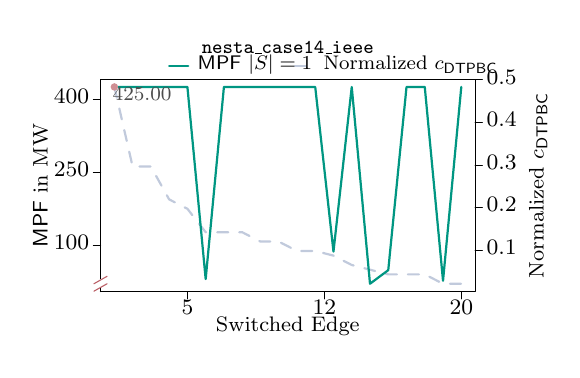
\begin{tikzpicture}[x=1pt,y=1pt]
\definecolor{fillColor}{RGB}{255,255,255}
\path[use as bounding box,fill=fillColor,fill opacity=0.00] (0,0) rectangle (440.85,271.01);
\begin{scope}
\path[clip] (  0.00,  0.00) rectangle (440.85,271.01);
\definecolor{drawColor}{RGB}{193,202,220}

\path[draw=drawColor,line width= 0.8pt,dash pattern=on 4pt off 4pt ,line join=round,line cap=round] ( 72.86,221.20) --
	( 88.20,154.26) --
	(103.55,154.26) --
	(118.89,126.69) --
	(134.23,118.82) --
	(149.58, 99.13) --
	(164.92, 99.13) --
	(180.26, 99.13) --
	(195.61, 91.25) --
	(210.95, 91.25) --
	(226.30, 83.38) --
	(241.64, 83.38) --
	(256.98, 79.44) --
	(272.33, 71.57) --
	(287.67, 67.63) --
	(303.01, 63.69) --
	(318.36, 63.69) --
	(333.70, 63.69) --
	(349.04, 55.82) --
	(364.39, 55.82);
\end{scope}
\begin{scope}
\path[clip] (  0.00,  0.00) rectangle (440.85,271.01);
\definecolor{drawColor}{RGB}{0,0,0}

\path[draw=drawColor,line width= 0.4pt,line join=round,line cap=round] ( 61.20, 49.20) --
	(376.05, 49.20) --
	(376.05,227.81) --
	( 61.20,227.81) --
	( 61.20, 49.20);
\end{scope}
\begin{scope}
\path[clip] (  0.00,  0.00) rectangle (440.85,271.01);
\definecolor{drawColor}{RGB}{0,0,0}

\path[draw=drawColor,line width= 0.4pt,line join=round,line cap=round] (376.05, 83.77) -- (376.05,227.10);

\path[draw=drawColor,line width= 0.4pt,line join=round,line cap=round] (376.05, 83.77) -- (382.05, 83.77);

\path[draw=drawColor,line width= 0.4pt,line join=round,line cap=round] (376.05,119.61) -- (382.05,119.61);

\path[draw=drawColor,line width= 0.4pt,line join=round,line cap=round] (376.05,155.44) -- (382.05,155.44);

\path[draw=drawColor,line width= 0.4pt,line join=round,line cap=round] (376.05,191.27) -- (382.05,191.27);

\path[draw=drawColor,line width= 0.4pt,line join=round,line cap=round] (376.05,227.10) -- (382.05,227.10);

\node[text=drawColor,anchor=base west,inner sep=0pt, outer sep=0pt, scale=  1.00] at (385.65, 80.33) {0.1};

\node[text=drawColor,anchor=base west,inner sep=0pt, outer sep=0pt, scale=  1.00] at (385.65,116.16) {0.2};

\node[text=drawColor,anchor=base west,inner sep=0pt, outer sep=0pt, scale=  1.00] at (385.65,151.99) {0.3};

\node[text=drawColor,anchor=base west,inner sep=0pt, outer sep=0pt, scale=  1.00] at (385.65,187.83) {0.4};

\node[text=drawColor,anchor=base west,inner sep=0pt, outer sep=0pt, scale=  1.00] at (385.65,223.66) {0.5};
\end{scope}
\begin{scope}
\path[clip] (  0.00,  0.00) rectangle (440.85,271.01);
\definecolor{drawColor}{RGB}{0,150,130}

\path[draw=drawColor,line width= 0.8pt,line join=round,line cap=round] (118.89,238.60) -- (134.91,238.60);
\definecolor{drawColor}{RGB}{193,202,220}

\path[draw=drawColor,line width= 0.8pt,dash pattern=on 4pt off 4pt ,line join=round,line cap=round] (224.63,238.60) -- (240.65,238.60);
\definecolor{drawColor}{RGB}{0,0,0}

\node[text=drawColor,anchor=base,inner sep=0pt, outer sep=0pt, scale=  0.89] at (218.62,249.28) {\texttt{nesta\_case14\_ieee}};

\node[text=drawColor,anchor=base west,inner sep=0pt, outer sep=0pt, scale=  0.89] at (142.92,235.54) {$\mathsf{MPF}~|S|=1$};

\node[text=drawColor,anchor=base west,inner sep=0pt, outer sep=0pt, scale=  0.89] at (248.66,235.54) {Normalized~$c_\mathsf{DTPBC}$};
\end{scope}
\begin{scope}
\path[clip] (  0.00,  0.00) rectangle (440.85,271.01);
\definecolor{drawColor}{RGB}{0,0,0}

\path[draw=drawColor,line width= 0.4pt,line join=round,line cap=round] ( 61.20, 87.92) -- ( 61.20,210.95);

\path[draw=drawColor,line width= 0.4pt,line join=round,line cap=round] ( 61.20, 87.92) -- ( 55.20, 87.92);

\path[draw=drawColor,line width= 0.4pt,line join=round,line cap=round] ( 61.20,149.43) -- ( 55.20,149.43);

\path[draw=drawColor,line width= 0.4pt,line join=round,line cap=round] ( 61.20,210.95) -- ( 55.20,210.95);

\node[text=drawColor,anchor=base east,inner sep=0pt, outer sep=0pt, scale=  1.00] at ( 51.60, 84.48) {100};

\node[text=drawColor,anchor=base east,inner sep=0pt, outer sep=0pt, scale=  1.00] at ( 51.60,145.99) {250};

\node[text=drawColor,anchor=base east,inner sep=0pt, outer sep=0pt, scale=  1.00] at ( 51.60,207.50) {400};
\end{scope}
\begin{scope}
\path[clip] (  0.00,  0.00) rectangle (440.85,271.01);
\definecolor{drawColor}{RGB}{255,255,255}
\definecolor{fillColor}{RGB}{255,255,255}

\path[draw=drawColor,line width= 0.4pt,line join=round,line cap=round,fill=fillColor] ( 55.69, 52.69) rectangle ( 66.71, 58.94);
\definecolor{drawColor}{RGB}{188,97,104}

\path[draw=drawColor,line width= 0.4pt,line join=round,line cap=round] ( 55.69, 49.56) -- ( 66.71, 55.82);

\path[draw=drawColor,line width= 0.4pt,line join=round,line cap=round] ( 55.69, 55.82) -- ( 66.71, 62.07);
\end{scope}
\begin{scope}
\path[clip] ( 61.20, 49.20) rectangle (376.05,227.81);
\definecolor{drawColor}{RGB}{0,150,130}

\path[draw=drawColor,line width= 0.8pt,line join=round,line cap=round] ( 72.86,221.20) --
	( 88.20,221.20) --
	(103.55,221.20) --
	(118.89,221.20) --
	(134.23,221.20) --
	(149.58, 59.77) --
	(164.92,221.20) --
	(180.26,221.20) --
	(195.61,221.20) --
	(210.95,221.20) --
	(226.30,221.20) --
	(241.64,221.20) --
	(256.98, 82.80) --
	(272.33,221.20) --
	(287.67, 55.82) --
	(303.01, 67.23) --
	(318.36,221.20) --
	(333.70,221.20) --
	(349.04, 58.28) --
	(364.39,221.20);
\end{scope}
\begin{scope}
\path[clip] ( 61.20, 49.20) rectangle (376.05,227.81);
\definecolor{fillColor}{RGB}{207,142,147}

\path[fill=fillColor] ( 72.86,221.20) circle (  3.15);
\end{scope}
\begin{scope}
\path[clip] ( 61.20, 49.20) rectangle (376.05,227.81);
\definecolor{drawColor}{gray}{0.30}

\node[text=drawColor,anchor=base,inner sep=0pt, outer sep=0pt, scale=  0.90] at ( 96.18,210.04) {425.00};
\end{scope}
\begin{scope}
\path[clip] (  0.00,  0.00) rectangle (440.85,271.01);
\definecolor{drawColor}{RGB}{0,0,0}

\path[draw=drawColor,line width= 0.4pt,line join=round,line cap=round] (134.23, 49.20) -- (364.39, 49.20);

\path[draw=drawColor,line width= 0.4pt,line join=round,line cap=round] (134.23, 49.20) -- (134.23, 43.20);

\path[draw=drawColor,line width= 0.4pt,line join=round,line cap=round] (249.31, 49.20) -- (249.31, 43.20);

\path[draw=drawColor,line width= 0.4pt,line join=round,line cap=round] (364.39, 49.20) -- (364.39, 43.20);

\node[text=drawColor,anchor=base,inner sep=0pt, outer sep=0pt, scale=  1.00] at (134.23, 30.00) {5};

\node[text=drawColor,anchor=base,inner sep=0pt, outer sep=0pt, scale=  1.00] at (249.31, 30.00) {12};

\node[text=drawColor,anchor=base,inner sep=0pt, outer sep=0pt, scale=  1.00] at (364.39, 30.00) {20};

\node[text=drawColor,anchor=base,inner sep=0pt, outer sep=0pt, scale=  0.95] at (218.62, 15.60) {Switched Edge};

\node[text=drawColor,rotate= 90.00,anchor=base,inner sep=0pt, outer sep=0pt, scale=  0.95] at ( 16.80,138.51) {$\mathsf{MPF}$ in~$\mathrm{MW}$};

\node[text=drawColor,rotate= 90.00,anchor=base,inner sep=0pt, outer sep=0pt, scale=  0.95] at (433.65,138.51) {Normalized~$c_\mathsf{DTPBC}$};
\end{scope}
\end{tikzpicture}
%
    \label{plot:SwitchingBetweenness_nesta_case14_ieee_dtpbc_mpf_cutY}%
  \end{subfigure}%
  \hfill
  \begin{subfigure}[t]{.5\textwidth}
    \centering
    % Created by tikzDevice version 0.10.1 on 2018-01-31 10:27:37
% !TEX encoding = UTF-8 Unicode
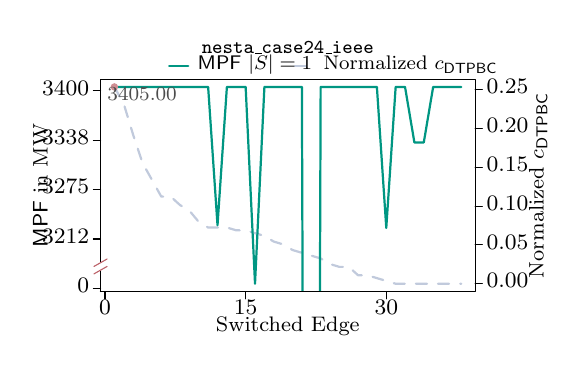
\begin{tikzpicture}[x=1pt,y=1pt]
\definecolor{fillColor}{RGB}{255,255,255}
\path[use as bounding box,fill=fillColor,fill opacity=0.00] (0,0) rectangle (440.85,271.01);
\begin{scope}
\path[clip] (  0.00,  0.00) rectangle (440.85,271.01);
\definecolor{drawColor}{RGB}{193,202,220}

\path[draw=drawColor,line width= 0.8pt,dash pattern=on 4pt off 4pt ,line join=round,line cap=round] ( 72.86,221.20) --
	( 80.74,207.02) --
	( 88.62,181.03) --
	( 96.50,157.41) --
	(104.38,143.23) --
	(112.26,129.06) --
	(120.14,129.06) --
	(128.01,121.97) --
	(135.89,117.24) --
	(143.77,107.79) --
	(151.65,103.07) --
	(159.53,103.07) --
	(167.41,103.07) --
	(175.29,100.70) --
	(183.17,100.70) --
	(191.05, 98.34) --
	(198.93, 95.98) --
	(206.80, 91.25) --
	(214.68, 88.89) --
	(222.56, 84.17) --
	(230.44, 81.80) --
	(238.32, 79.44) --
	(246.20, 77.08) --
	(254.08, 72.35) --
	(261.96, 69.99) --
	(269.84, 69.99) --
	(277.72, 62.90) --
	(285.60, 62.90) --
	(293.47, 60.54) --
	(301.35, 58.18) --
	(309.23, 55.82) --
	(317.11, 55.82) --
	(324.99, 55.82) --
	(332.87, 55.82) --
	(340.75, 55.82) --
	(348.63, 55.82) --
	(356.51, 55.82) --
	(364.39, 55.82);
\end{scope}
\begin{scope}
\path[clip] (  0.00,  0.00) rectangle (440.85,271.01);
\definecolor{drawColor}{RGB}{0,0,0}

\path[draw=drawColor,line width= 0.4pt,line join=round,line cap=round] ( 61.20, 49.20) --
	(376.05, 49.20) --
	(376.05,227.81) --
	( 61.20,227.81) --
	( 61.20, 49.20);
\end{scope}
\begin{scope}
\path[clip] (  0.00,  0.00) rectangle (440.85,271.01);
\definecolor{drawColor}{RGB}{0,0,0}

\path[draw=drawColor,line width= 0.4pt,line join=round,line cap=round] (376.05, 55.82) -- (376.05,218.83);

\path[draw=drawColor,line width= 0.4pt,line join=round,line cap=round] (376.05, 55.82) -- (382.05, 55.82);

\path[draw=drawColor,line width= 0.4pt,line join=round,line cap=round] (376.05, 88.42) -- (382.05, 88.42);

\path[draw=drawColor,line width= 0.4pt,line join=round,line cap=round] (376.05,121.02) -- (382.05,121.02);

\path[draw=drawColor,line width= 0.4pt,line join=round,line cap=round] (376.05,153.63) -- (382.05,153.63);

\path[draw=drawColor,line width= 0.4pt,line join=round,line cap=round] (376.05,186.23) -- (382.05,186.23);

\path[draw=drawColor,line width= 0.4pt,line join=round,line cap=round] (376.05,218.83) -- (382.05,218.83);

\node[text=drawColor,anchor=base west,inner sep=0pt, outer sep=0pt, scale=  1.00] at (385.65, 52.37) {0.00};

\node[text=drawColor,anchor=base west,inner sep=0pt, outer sep=0pt, scale=  1.00] at (385.65, 84.98) {0.05};

\node[text=drawColor,anchor=base west,inner sep=0pt, outer sep=0pt, scale=  1.00] at (385.65,117.58) {0.10};

\node[text=drawColor,anchor=base west,inner sep=0pt, outer sep=0pt, scale=  1.00] at (385.65,150.18) {0.15};

\node[text=drawColor,anchor=base west,inner sep=0pt, outer sep=0pt, scale=  1.00] at (385.65,182.79) {0.20};

\node[text=drawColor,anchor=base west,inner sep=0pt, outer sep=0pt, scale=  1.00] at (385.65,215.39) {0.25};
\end{scope}
\begin{scope}
\path[clip] (  0.00,  0.00) rectangle (440.85,271.01);
\definecolor{drawColor}{RGB}{0,150,130}

\path[draw=drawColor,line width= 0.8pt,line join=round,line cap=round] (118.89,238.60) -- (134.91,238.60);
\definecolor{drawColor}{RGB}{193,202,220}

\path[draw=drawColor,line width= 0.8pt,dash pattern=on 4pt off 4pt ,line join=round,line cap=round] (224.63,238.60) -- (240.65,238.60);
\definecolor{drawColor}{RGB}{0,0,0}

\node[text=drawColor,anchor=base,inner sep=0pt, outer sep=0pt, scale=  0.89] at (218.62,249.28) {\texttt{nesta\_case24\_ieee}};

\node[text=drawColor,anchor=base west,inner sep=0pt, outer sep=0pt, scale=  0.89] at (142.92,235.54) {$\mathsf{MPF}~|S|=1$};

\node[text=drawColor,anchor=base west,inner sep=0pt, outer sep=0pt, scale=  0.89] at (248.66,235.54) {Normalized~$c_\mathsf{DTPBC}$};
\end{scope}
\begin{scope}
\path[clip] (  0.00,  0.00) rectangle (440.85,271.01);
\definecolor{drawColor}{RGB}{0,0,0}

\path[draw=drawColor,line width= 0.4pt,line join=round,line cap=round] ( 61.20, 51.91) -- ( 61.20,217.88);

\path[draw=drawColor,line width= 0.4pt,line join=round,line cap=round] ( 61.20, 51.91) -- ( 55.20, 51.91);

\path[draw=drawColor,line width= 0.4pt,line join=round,line cap=round] ( 61.20, 93.40) -- ( 55.20, 93.40);

\path[draw=drawColor,line width= 0.4pt,line join=round,line cap=round] ( 61.20,134.89) -- ( 55.20,134.89);

\path[draw=drawColor,line width= 0.4pt,line join=round,line cap=round] ( 61.20,176.39) -- ( 55.20,176.39);

\path[draw=drawColor,line width= 0.4pt,line join=round,line cap=round] ( 61.20,217.88) -- ( 55.20,217.88);

\node[text=drawColor,anchor=base east,inner sep=0pt, outer sep=0pt, scale=  1.00] at ( 51.60, 48.47) {0};

\node[text=drawColor,anchor=base east,inner sep=0pt, outer sep=0pt, scale=  1.00] at ( 51.60, 89.96) {3212};

\node[text=drawColor,anchor=base east,inner sep=0pt, outer sep=0pt, scale=  1.00] at ( 51.60,131.45) {3275};

\node[text=drawColor,anchor=base east,inner sep=0pt, outer sep=0pt, scale=  1.00] at ( 51.60,172.94) {3338};

\node[text=drawColor,anchor=base east,inner sep=0pt, outer sep=0pt, scale=  1.00] at ( 51.60,214.43) {3400};
\end{scope}
\begin{scope}
\path[clip] (  0.00,  0.00) rectangle (440.85,271.01);
\definecolor{drawColor}{RGB}{255,255,255}
\definecolor{fillColor}{RGB}{255,255,255}

\path[draw=drawColor,line width= 0.4pt,line join=round,line cap=round,fill=fillColor] ( 55.69, 67.23) rectangle ( 66.71, 73.48);
\definecolor{drawColor}{RGB}{188,97,104}

\path[draw=drawColor,line width= 0.4pt,line join=round,line cap=round] ( 55.69, 64.10) -- ( 66.71, 70.35);

\path[draw=drawColor,line width= 0.4pt,line join=round,line cap=round] ( 55.69, 70.35) -- ( 66.71, 76.60);
\end{scope}
\begin{scope}
\path[clip] ( 61.20, 49.20) rectangle (376.05,227.81);
\definecolor{drawColor}{RGB}{0,150,130}

\path[draw=drawColor,line width= 0.8pt,line join=round,line cap=round] ( 72.86,221.20) --
	( 80.74,221.20) --
	( 88.62,221.20) --
	( 96.50,221.20) --
	(104.38,221.20) --
	(112.26,221.20) --
	(120.14,221.20) --
	(128.01,221.20) --
	(135.89,221.20) --
	(143.77,221.20) --
	(151.65,221.20) --
	(159.53,105.02) --
	(167.41,221.20) --
	(175.29,221.20) --
	(183.17,221.20) --
	(191.05, 55.82) --
	(198.93,221.20) --
	(206.80,221.20) --
	(214.68,221.20) --
	(222.56,221.20) --
	(230.44,221.20) --
	(231.21,  0.00);

\path[draw=drawColor,line width= 0.8pt,line join=round,line cap=round] (245.43,  0.00) --
	(246.20,221.20) --
	(254.08,221.20) --
	(261.96,221.20) --
	(269.84,221.20) --
	(277.72,221.20) --
	(285.60,221.20) --
	(293.47,221.20) --
	(301.35,102.74) --
	(309.23,221.20) --
	(317.11,221.20) --
	(324.99,174.53) --
	(332.87,174.53) --
	(340.75,221.20) --
	(348.63,221.20) --
	(356.51,221.20) --
	(364.39,221.20);
\end{scope}
\begin{scope}
\path[clip] ( 61.20, 49.20) rectangle (376.05,227.81);
\definecolor{fillColor}{RGB}{207,142,147}

\path[fill=fillColor] ( 72.86,221.20) circle (  3.15);
\end{scope}
\begin{scope}
\path[clip] ( 61.20, 49.20) rectangle (376.05,227.81);
\definecolor{drawColor}{gray}{0.30}

\node[text=drawColor,anchor=base,inner sep=0pt, outer sep=0pt, scale=  0.90] at ( 96.18,210.04) {3405.00};
\end{scope}
\begin{scope}
\path[clip] (  0.00,  0.00) rectangle (440.85,271.01);
\definecolor{drawColor}{RGB}{0,0,0}

\path[draw=drawColor,line width= 0.4pt,line join=round,line cap=round] ( 64.98, 49.20) -- (301.35, 49.20);

\path[draw=drawColor,line width= 0.4pt,line join=round,line cap=round] ( 64.98, 49.20) -- ( 64.98, 43.20);

\path[draw=drawColor,line width= 0.4pt,line join=round,line cap=round] (183.17, 49.20) -- (183.17, 43.20);

\path[draw=drawColor,line width= 0.4pt,line join=round,line cap=round] (301.35, 49.20) -- (301.35, 43.20);

\node[text=drawColor,anchor=base,inner sep=0pt, outer sep=0pt, scale=  1.00] at ( 64.98, 30.00) {0};

\node[text=drawColor,anchor=base,inner sep=0pt, outer sep=0pt, scale=  1.00] at (183.17, 30.00) {15};

\node[text=drawColor,anchor=base,inner sep=0pt, outer sep=0pt, scale=  1.00] at (301.35, 30.00) {30};

\node[text=drawColor,anchor=base,inner sep=0pt, outer sep=0pt, scale=  0.95] at (218.62, 15.60) {Switched Edge};

\node[text=drawColor,rotate= 90.00,anchor=base,inner sep=0pt, outer sep=0pt, scale=  0.95] at ( 16.80,138.51) {$\mathsf{MPF}$ in~$\mathrm{MW}$};

\node[text=drawColor,rotate= 90.00,anchor=base,inner sep=0pt, outer sep=0pt, scale=  0.95] at (433.65,138.51) {Normalized~$c_\mathsf{DTPBC}$};
\end{scope}
\end{tikzpicture}
%
    \label{plot:SwitchingBetweenness_nesta_case24_ieee_rts_dtpbc_mpf_cutY}%
  \end{subfigure}%
% 
  \caption{Results of the simulations for the~\gls{dtp} betweenness centrality
  on \texttt{nesta\_case3\_lmbd} to \texttt{nesta\_case24\_ieee\_rts}.
  }%
  % 
  \label{fig:Switching_Betweenness_Centrality_Plot_Cut_Y_3_to_24}%
\end{figure}%
%

%%%%%%%%%%%%%%%%%%%%%%%%%%%%%%%%%%%%%%%%%%%%%%%%%%%%%%%%%%%%%%%%%%%%%%%%%%%%%%%%
\newpage
%
\begin{figure}[H]%
  %
  \begin{subfigure}[t]{.5\textwidth}%
    \centering%
    % Created by tikzDevice version 0.10.1 on 2018-01-31 10:28:08
% !TEX encoding = UTF-8 Unicode
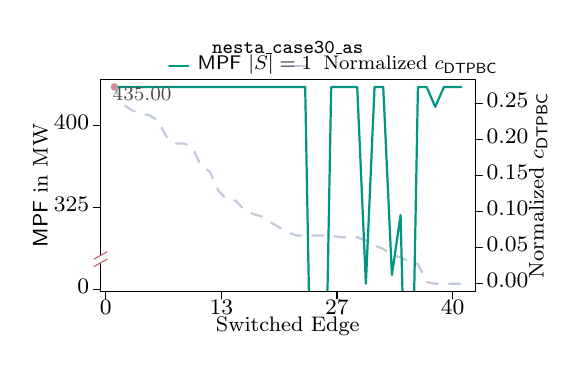
\begin{tikzpicture}[x=1pt,y=1pt]
\definecolor{fillColor}{RGB}{255,255,255}
\path[use as bounding box,fill=fillColor,fill opacity=0.00] (0,0) rectangle (440.85,271.01);
\begin{scope}
\path[clip] (  0.00,  0.00) rectangle (440.85,271.01);
\definecolor{drawColor}{RGB}{193,202,220}

\path[draw=drawColor,line width= 0.8pt,dash pattern=on 4pt off 4pt ,line join=round,line cap=round] ( 72.86,221.20) --
	( 80.15,206.54) --
	( 87.44,201.66) --
	( 94.73,198.87) --
	(102.01,197.47) --
	(109.30,193.28) --
	(116.59,179.33) --
	(123.88,173.75) --
	(131.17,173.75) --
	(138.45,170.26) --
	(145.74,154.90) --
	(153.03,150.02) --
	(160.32,133.97) --
	(167.61,126.29) --
	(174.89,125.60) --
	(182.18,117.92) --
	(189.47,114.43) --
	(196.76,112.34) --
	(204.05,107.45) --
	(211.34,103.27) --
	(218.62, 99.08) --
	(225.91, 96.29) --
	(233.20, 96.29) --
	(240.49, 96.29) --
	(247.78, 96.29) --
	(255.06, 96.29) --
	(262.35, 94.89) --
	(269.64, 94.89) --
	(276.93, 94.89) --
	(284.22, 92.10) --
	(291.50, 87.91) --
	(298.79, 85.12) --
	(306.08, 79.54) --
	(313.37, 78.15) --
	(320.66, 73.96) --
	(327.95, 72.56) --
	(335.23, 57.21) --
	(342.52, 55.82) --
	(349.81, 55.82) --
	(357.10, 55.82) --
	(364.39, 55.82);
\end{scope}
\begin{scope}
\path[clip] (  0.00,  0.00) rectangle (440.85,271.01);
\definecolor{drawColor}{RGB}{0,0,0}

\path[draw=drawColor,line width= 0.4pt,line join=round,line cap=round] ( 61.20, 49.20) --
	(376.05, 49.20) --
	(376.05,227.81) --
	( 61.20,227.81) --
	( 61.20, 49.20);
\end{scope}
\begin{scope}
\path[clip] (  0.00,  0.00) rectangle (440.85,271.01);
\definecolor{drawColor}{RGB}{0,0,0}

\path[draw=drawColor,line width= 0.4pt,line join=round,line cap=round] (376.05, 55.82) -- (376.05,207.59);

\path[draw=drawColor,line width= 0.4pt,line join=round,line cap=round] (376.05, 55.82) -- (382.05, 55.82);

\path[draw=drawColor,line width= 0.4pt,line join=round,line cap=round] (376.05, 86.17) -- (382.05, 86.17);

\path[draw=drawColor,line width= 0.4pt,line join=round,line cap=round] (376.05,116.53) -- (382.05,116.53);

\path[draw=drawColor,line width= 0.4pt,line join=round,line cap=round] (376.05,146.88) -- (382.05,146.88);

\path[draw=drawColor,line width= 0.4pt,line join=round,line cap=round] (376.05,177.23) -- (382.05,177.23);

\path[draw=drawColor,line width= 0.4pt,line join=round,line cap=round] (376.05,207.59) -- (382.05,207.59);

\node[text=drawColor,anchor=base west,inner sep=0pt, outer sep=0pt, scale=  1.00] at (385.65, 52.37) {0.00};

\node[text=drawColor,anchor=base west,inner sep=0pt, outer sep=0pt, scale=  1.00] at (385.65, 82.73) {0.05};

\node[text=drawColor,anchor=base west,inner sep=0pt, outer sep=0pt, scale=  1.00] at (385.65,113.08) {0.10};

\node[text=drawColor,anchor=base west,inner sep=0pt, outer sep=0pt, scale=  1.00] at (385.65,143.44) {0.15};

\node[text=drawColor,anchor=base west,inner sep=0pt, outer sep=0pt, scale=  1.00] at (385.65,173.79) {0.20};

\node[text=drawColor,anchor=base west,inner sep=0pt, outer sep=0pt, scale=  1.00] at (385.65,204.15) {0.25};
\end{scope}
\begin{scope}
\path[clip] (  0.00,  0.00) rectangle (440.85,271.01);
\definecolor{drawColor}{RGB}{0,150,130}

\path[draw=drawColor,line width= 0.8pt,line join=round,line cap=round] (118.89,238.60) -- (134.91,238.60);
\definecolor{drawColor}{RGB}{193,202,220}

\path[draw=drawColor,line width= 0.8pt,dash pattern=on 4pt off 4pt ,line join=round,line cap=round] (224.63,238.60) -- (240.65,238.60);
\definecolor{drawColor}{RGB}{0,0,0}

\node[text=drawColor,anchor=base,inner sep=0pt, outer sep=0pt, scale=  0.89] at (218.62,249.28) {\texttt{nesta\_case30\_as}};

\node[text=drawColor,anchor=base west,inner sep=0pt, outer sep=0pt, scale=  0.89] at (142.92,235.54) {$\mathsf{MPF}~|S|=1$};

\node[text=drawColor,anchor=base west,inner sep=0pt, outer sep=0pt, scale=  0.89] at (248.66,235.54) {Normalized~$c_\mathsf{DTPBC}$};
\end{scope}
\begin{scope}
\path[clip] (  0.00,  0.00) rectangle (440.85,271.01);
\definecolor{drawColor}{RGB}{0,0,0}

\path[draw=drawColor,line width= 0.4pt,line join=round,line cap=round] ( 61.20, 50.90) -- ( 61.20,188.98);

\path[draw=drawColor,line width= 0.4pt,line join=round,line cap=round] ( 61.20, 50.90) -- ( 55.20, 50.90);

\path[draw=drawColor,line width= 0.4pt,line join=round,line cap=round] ( 61.20,119.94) -- ( 55.20,119.94);

\path[draw=drawColor,line width= 0.4pt,line join=round,line cap=round] ( 61.20,188.98) -- ( 55.20,188.98);

\node[text=drawColor,anchor=base east,inner sep=0pt, outer sep=0pt, scale=  1.00] at ( 51.60, 47.45) {0};

\node[text=drawColor,anchor=base east,inner sep=0pt, outer sep=0pt, scale=  1.00] at ( 51.60,116.49) {325};

\node[text=drawColor,anchor=base east,inner sep=0pt, outer sep=0pt, scale=  1.00] at ( 51.60,185.53) {400};
\end{scope}
\begin{scope}
\path[clip] (  0.00,  0.00) rectangle (440.85,271.01);
\definecolor{drawColor}{RGB}{255,255,255}
\definecolor{fillColor}{RGB}{255,255,255}

\path[draw=drawColor,line width= 0.4pt,line join=round,line cap=round,fill=fillColor] ( 55.69, 73.34) rectangle ( 66.71, 79.59);
\definecolor{drawColor}{RGB}{188,97,104}

\path[draw=drawColor,line width= 0.4pt,line join=round,line cap=round] ( 55.69, 70.22) -- ( 66.71, 76.47);

\path[draw=drawColor,line width= 0.4pt,line join=round,line cap=round] ( 55.69, 76.47) -- ( 66.71, 82.72);
\end{scope}
\begin{scope}
\path[clip] ( 61.20, 49.20) rectangle (376.05,227.81);
\definecolor{drawColor}{RGB}{0,150,130}

\path[draw=drawColor,line width= 0.8pt,line join=round,line cap=round] ( 72.86,221.20) --
	( 80.15,221.20) --
	( 87.44,221.20) --
	( 94.73,221.20) --
	(102.01,221.20) --
	(109.30,221.20) --
	(116.59,221.20) --
	(123.88,221.20) --
	(131.17,221.20) --
	(138.45,221.20) --
	(145.74,221.20) --
	(153.03,221.20) --
	(160.32,221.20) --
	(167.61,221.20) --
	(174.89,221.20) --
	(182.18,221.20) --
	(189.47,221.20) --
	(196.76,221.20) --
	(204.05,221.20) --
	(211.34,221.20) --
	(218.62,221.20) --
	(225.91,221.20) --
	(233.20,221.20) --
	(237.23,  0.00);

\path[draw=drawColor,line width= 0.8pt,line join=round,line cap=round] (251.04,  0.00) --
	(255.06,221.20) --
	(262.35,221.20) --
	(269.64,221.20) --
	(276.93,221.20) --
	(284.22, 55.82) --
	(291.50,221.20) --
	(298.79,221.20) --
	(306.08, 63.18) --
	(313.37,113.51) --
	(316.19,  0.00);

\path[draw=drawColor,line width= 0.8pt,line join=round,line cap=round] (323.92,  0.00) --
	(327.95,221.20) --
	(335.23,221.20) --
	(342.52,204.50) --
	(349.81,221.20) --
	(357.10,221.20) --
	(364.39,221.20);
\end{scope}
\begin{scope}
\path[clip] ( 61.20, 49.20) rectangle (376.05,227.81);
\definecolor{fillColor}{RGB}{207,142,147}

\path[fill=fillColor] ( 72.86,221.20) circle (  3.15);
\end{scope}
\begin{scope}
\path[clip] ( 61.20, 49.20) rectangle (376.05,227.81);
\definecolor{drawColor}{gray}{0.30}

\node[text=drawColor,anchor=base,inner sep=0pt, outer sep=0pt, scale=  0.90] at ( 96.18,210.04) {435.00};
\end{scope}
\begin{scope}
\path[clip] (  0.00,  0.00) rectangle (440.85,271.01);
\definecolor{drawColor}{RGB}{0,0,0}

\path[draw=drawColor,line width= 0.4pt,line join=round,line cap=round] ( 65.57, 49.20) -- (357.10, 49.20);

\path[draw=drawColor,line width= 0.4pt,line join=round,line cap=round] ( 65.57, 49.20) -- ( 65.57, 43.20);

\path[draw=drawColor,line width= 0.4pt,line join=round,line cap=round] (162.75, 49.20) -- (162.75, 43.20);

\path[draw=drawColor,line width= 0.4pt,line join=round,line cap=round] (259.92, 49.20) -- (259.92, 43.20);

\path[draw=drawColor,line width= 0.4pt,line join=round,line cap=round] (357.10, 49.20) -- (357.10, 43.20);

\node[text=drawColor,anchor=base,inner sep=0pt, outer sep=0pt, scale=  1.00] at ( 65.57, 30.00) {0};

\node[text=drawColor,anchor=base,inner sep=0pt, outer sep=0pt, scale=  1.00] at (162.75, 30.00) {13};

\node[text=drawColor,anchor=base,inner sep=0pt, outer sep=0pt, scale=  1.00] at (259.92, 30.00) {27};

\node[text=drawColor,anchor=base,inner sep=0pt, outer sep=0pt, scale=  1.00] at (357.10, 30.00) {40};

\node[text=drawColor,anchor=base,inner sep=0pt, outer sep=0pt, scale=  0.95] at (218.62, 15.60) {Switched Edge};

\node[text=drawColor,rotate= 90.00,anchor=base,inner sep=0pt, outer sep=0pt, scale=  0.95] at ( 16.80,138.51) {$\mathsf{MPF}$ in~$\mathrm{MW}$};

\node[text=drawColor,rotate= 90.00,anchor=base,inner sep=0pt, outer sep=0pt, scale=  0.95] at (433.65,138.51) {Normalized~$c_\mathsf{DTPBC}$};
\end{scope}
\end{tikzpicture}
%
    \label{plot:SwitchingBetweenness_nesta_case30_as_dtpbc_mpf_cutY}%
  \end{subfigure}%
  \hfill%
  %
  \begin{subfigure}[t]{.5\textwidth}%
    \centering%
    \input{switchplacement/plots/plot-SwitchingBetweenness_nesta_case30_fsr-dtpbc-mpf-cutY.tex}%
    \label{plot:SwitchingBetweenness_nesta_case30_fsr_dtpbc_mpf_cutY}%
  \end{subfigure}%

  %
  \begin{subfigure}[t]{.5\textwidth}%
    \centering%
    % Created by tikzDevice version 0.10.1 on 2018-01-31 10:28:13
% !TEX encoding = UTF-8 Unicode
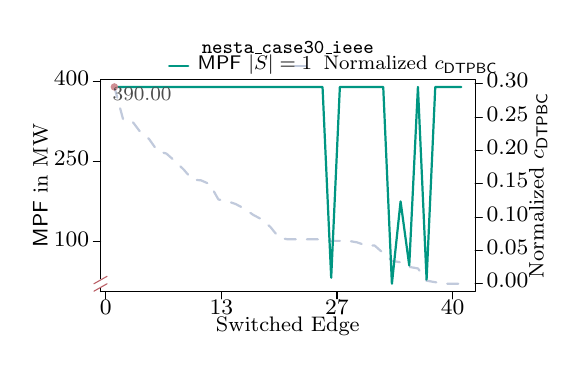
\begin{tikzpicture}[x=1pt,y=1pt]
\definecolor{fillColor}{RGB}{255,255,255}
\path[use as bounding box,fill=fillColor,fill opacity=0.00] (0,0) rectangle (440.85,271.01);
\begin{scope}
\path[clip] (  0.00,  0.00) rectangle (440.85,271.01);
\definecolor{drawColor}{RGB}{193,202,220}

\path[draw=drawColor,line width= 0.8pt,dash pattern=on 4pt off 4pt ,line join=round,line cap=round] ( 72.86,221.20) --
	( 80.15,194.17) --
	( 87.44,192.88) --
	( 94.73,183.23) --
	(102.01,177.44) --
	(109.30,167.14) --
	(116.59,165.21) --
	(123.88,158.78) --
	(131.17,151.70) --
	(138.45,143.33) --
	(145.74,142.69) --
	(153.03,139.47) --
	(160.32,126.60) --
	(167.61,125.31) --
	(174.89,122.74) --
	(182.18,118.88) --
	(189.47,113.73) --
	(196.76,109.87) --
	(204.05,103.44) --
	(211.34, 94.43) --
	(218.62, 93.14) --
	(225.91, 93.14) --
	(233.20, 93.14) --
	(240.49, 93.14) --
	(247.78, 93.14) --
	(255.06, 91.85) --
	(262.35, 91.85) --
	(269.64, 91.85) --
	(276.93, 90.56) --
	(284.22, 87.99) --
	(291.50, 87.99) --
	(298.79, 81.56) --
	(306.08, 75.12) --
	(313.37, 73.83) --
	(320.66, 69.97) --
	(327.95, 68.69) --
	(335.23, 58.39) --
	(342.52, 57.10) --
	(349.81, 55.82) --
	(357.10, 55.82) --
	(364.39, 55.82);
\end{scope}
\begin{scope}
\path[clip] (  0.00,  0.00) rectangle (440.85,271.01);
\definecolor{drawColor}{RGB}{0,0,0}

\path[draw=drawColor,line width= 0.4pt,line join=round,line cap=round] ( 61.20, 49.20) --
	(376.05, 49.20) --
	(376.05,227.81) --
	( 61.20,227.81) --
	( 61.20, 49.20);
\end{scope}
\begin{scope}
\path[clip] (  0.00,  0.00) rectangle (440.85,271.01);
\definecolor{drawColor}{RGB}{0,0,0}

\path[draw=drawColor,line width= 0.4pt,line join=round,line cap=round] (376.05, 55.82) -- (376.05,223.77);

\path[draw=drawColor,line width= 0.4pt,line join=round,line cap=round] (376.05, 55.82) -- (382.05, 55.82);

\path[draw=drawColor,line width= 0.4pt,line join=round,line cap=round] (376.05, 83.81) -- (382.05, 83.81);

\path[draw=drawColor,line width= 0.4pt,line join=round,line cap=round] (376.05,111.80) -- (382.05,111.80);

\path[draw=drawColor,line width= 0.4pt,line join=round,line cap=round] (376.05,139.79) -- (382.05,139.79);

\path[draw=drawColor,line width= 0.4pt,line join=round,line cap=round] (376.05,167.79) -- (382.05,167.79);

\path[draw=drawColor,line width= 0.4pt,line join=round,line cap=round] (376.05,195.78) -- (382.05,195.78);

\path[draw=drawColor,line width= 0.4pt,line join=round,line cap=round] (376.05,223.77) -- (382.05,223.77);

\node[text=drawColor,anchor=base west,inner sep=0pt, outer sep=0pt, scale=  1.00] at (385.65, 52.37) {0.00};

\node[text=drawColor,anchor=base west,inner sep=0pt, outer sep=0pt, scale=  1.00] at (385.65, 80.36) {0.05};

\node[text=drawColor,anchor=base west,inner sep=0pt, outer sep=0pt, scale=  1.00] at (385.65,108.36) {0.10};

\node[text=drawColor,anchor=base west,inner sep=0pt, outer sep=0pt, scale=  1.00] at (385.65,136.35) {0.15};

\node[text=drawColor,anchor=base west,inner sep=0pt, outer sep=0pt, scale=  1.00] at (385.65,164.34) {0.20};

\node[text=drawColor,anchor=base west,inner sep=0pt, outer sep=0pt, scale=  1.00] at (385.65,192.34) {0.25};

\node[text=drawColor,anchor=base west,inner sep=0pt, outer sep=0pt, scale=  1.00] at (385.65,220.33) {0.30};
\end{scope}
\begin{scope}
\path[clip] (  0.00,  0.00) rectangle (440.85,271.01);
\definecolor{drawColor}{RGB}{0,150,130}

\path[draw=drawColor,line width= 0.8pt,line join=round,line cap=round] (118.89,238.60) -- (134.91,238.60);
\definecolor{drawColor}{RGB}{193,202,220}

\path[draw=drawColor,line width= 0.8pt,dash pattern=on 4pt off 4pt ,line join=round,line cap=round] (224.63,238.60) -- (240.65,238.60);
\definecolor{drawColor}{RGB}{0,0,0}

\node[text=drawColor,anchor=base,inner sep=0pt, outer sep=0pt, scale=  0.89] at (218.62,249.28) {\texttt{nesta\_case30\_ieee}};

\node[text=drawColor,anchor=base west,inner sep=0pt, outer sep=0pt, scale=  0.89] at (142.92,235.54) {$\mathsf{MPF}~|S|=1$};

\node[text=drawColor,anchor=base west,inner sep=0pt, outer sep=0pt, scale=  0.89] at (248.66,235.54) {Normalized~$c_\mathsf{DTPBC}$};
\end{scope}
\begin{scope}
\path[clip] (  0.00,  0.00) rectangle (440.85,271.01);
\definecolor{drawColor}{RGB}{0,0,0}

\path[draw=drawColor,line width= 0.4pt,line join=round,line cap=round] ( 61.20, 90.98) -- ( 61.20,225.69);

\path[draw=drawColor,line width= 0.4pt,line join=round,line cap=round] ( 61.20, 90.98) -- ( 55.20, 90.98);

\path[draw=drawColor,line width= 0.4pt,line join=round,line cap=round] ( 61.20,158.33) -- ( 55.20,158.33);

\path[draw=drawColor,line width= 0.4pt,line join=round,line cap=round] ( 61.20,225.69) -- ( 55.20,225.69);

\node[text=drawColor,anchor=base east,inner sep=0pt, outer sep=0pt, scale=  1.00] at ( 51.60, 87.53) {100};

\node[text=drawColor,anchor=base east,inner sep=0pt, outer sep=0pt, scale=  1.00] at ( 51.60,154.89) {250};

\node[text=drawColor,anchor=base east,inner sep=0pt, outer sep=0pt, scale=  1.00] at ( 51.60,222.24) {400};
\end{scope}
\begin{scope}
\path[clip] (  0.00,  0.00) rectangle (440.85,271.01);
\definecolor{drawColor}{RGB}{255,255,255}
\definecolor{fillColor}{RGB}{255,255,255}

\path[draw=drawColor,line width= 0.4pt,line join=round,line cap=round,fill=fillColor] ( 55.69, 52.69) rectangle ( 66.71, 58.94);
\definecolor{drawColor}{RGB}{188,97,104}

\path[draw=drawColor,line width= 0.4pt,line join=round,line cap=round] ( 55.69, 49.56) -- ( 66.71, 55.82);

\path[draw=drawColor,line width= 0.4pt,line join=round,line cap=round] ( 55.69, 55.82) -- ( 66.71, 62.07);
\end{scope}
\begin{scope}
\path[clip] ( 61.20, 49.20) rectangle (376.05,227.81);
\definecolor{drawColor}{RGB}{0,150,130}

\path[draw=drawColor,line width= 0.8pt,line join=round,line cap=round] ( 72.86,221.20) --
	( 80.15,221.20) --
	( 87.44,221.20) --
	( 94.73,221.20) --
	(102.01,221.20) --
	(109.30,221.20) --
	(116.59,221.20) --
	(123.88,221.20) --
	(131.17,221.20) --
	(138.45,221.20) --
	(145.74,221.20) --
	(153.03,221.20) --
	(160.32,221.20) --
	(167.61,221.20) --
	(174.89,221.20) --
	(182.18,221.20) --
	(189.47,221.20) --
	(196.76,221.20) --
	(204.05,221.20) --
	(211.34,221.20) --
	(218.62,221.20) --
	(225.91,221.20) --
	(233.20,221.20) --
	(240.49,221.20) --
	(247.78,221.20) --
	(255.06, 60.87) --
	(262.35,221.20) --
	(269.64,221.20) --
	(276.93,221.20) --
	(284.22,221.20) --
	(291.50,221.20) --
	(298.79,221.20) --
	(306.08, 55.82) --
	(313.37,125.02) --
	(320.66, 71.19) --
	(327.95,221.20) --
	(335.23, 59.32) --
	(342.52,221.20) --
	(349.81,221.20) --
	(357.10,221.20) --
	(364.39,221.20);
\end{scope}
\begin{scope}
\path[clip] ( 61.20, 49.20) rectangle (376.05,227.81);
\definecolor{fillColor}{RGB}{207,142,147}

\path[fill=fillColor] ( 72.86,221.20) circle (  3.15);
\end{scope}
\begin{scope}
\path[clip] ( 61.20, 49.20) rectangle (376.05,227.81);
\definecolor{drawColor}{gray}{0.30}

\node[text=drawColor,anchor=base,inner sep=0pt, outer sep=0pt, scale=  0.90] at ( 96.18,210.04) {390.00};
\end{scope}
\begin{scope}
\path[clip] (  0.00,  0.00) rectangle (440.85,271.01);
\definecolor{drawColor}{RGB}{0,0,0}

\path[draw=drawColor,line width= 0.4pt,line join=round,line cap=round] ( 65.57, 49.20) -- (357.10, 49.20);

\path[draw=drawColor,line width= 0.4pt,line join=round,line cap=round] ( 65.57, 49.20) -- ( 65.57, 43.20);

\path[draw=drawColor,line width= 0.4pt,line join=round,line cap=round] (162.75, 49.20) -- (162.75, 43.20);

\path[draw=drawColor,line width= 0.4pt,line join=round,line cap=round] (259.92, 49.20) -- (259.92, 43.20);

\path[draw=drawColor,line width= 0.4pt,line join=round,line cap=round] (357.10, 49.20) -- (357.10, 43.20);

\node[text=drawColor,anchor=base,inner sep=0pt, outer sep=0pt, scale=  1.00] at ( 65.57, 30.00) {0};

\node[text=drawColor,anchor=base,inner sep=0pt, outer sep=0pt, scale=  1.00] at (162.75, 30.00) {13};

\node[text=drawColor,anchor=base,inner sep=0pt, outer sep=0pt, scale=  1.00] at (259.92, 30.00) {27};

\node[text=drawColor,anchor=base,inner sep=0pt, outer sep=0pt, scale=  1.00] at (357.10, 30.00) {40};

\node[text=drawColor,anchor=base,inner sep=0pt, outer sep=0pt, scale=  0.95] at (218.62, 15.60) {Switched Edge};

\node[text=drawColor,rotate= 90.00,anchor=base,inner sep=0pt, outer sep=0pt, scale=  0.95] at ( 16.80,138.51) {$\mathsf{MPF}$ in~$\mathrm{MW}$};

\node[text=drawColor,rotate= 90.00,anchor=base,inner sep=0pt, outer sep=0pt, scale=  0.95] at (433.65,138.51) {Normalized~$c_\mathsf{DTPBC}$};
\end{scope}
\end{tikzpicture}
%
    \label{plot:SwitchingBetweenness_nesta_case30_ieee_dtpbc_mpf_cutY}%
  \end{subfigure}%
  \hfill
  %
  \begin{subfigure}[t]{.5\textwidth}%
    \centering%
    % Created by tikzDevice version 0.10.1 on 2018-01-31 10:28:21
% !TEX encoding = UTF-8 Unicode
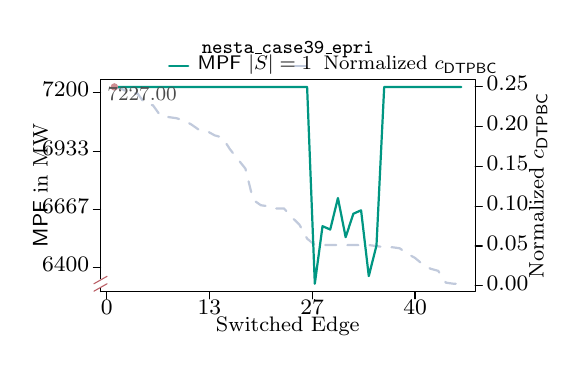
\begin{tikzpicture}[x=1pt,y=1pt]
\definecolor{fillColor}{RGB}{255,255,255}
\path[use as bounding box,fill=fillColor,fill opacity=0.00] (0,0) rectangle (440.85,271.01);
\begin{scope}
\path[clip] (  0.00,  0.00) rectangle (440.85,271.01);
\definecolor{drawColor}{RGB}{193,202,220}

\path[draw=drawColor,line width= 0.8pt,dash pattern=on 4pt off 4pt ,line join=round,line cap=round] ( 72.86,221.20) --
	( 79.34,219.39) --
	( 85.82,215.77) --
	( 92.30,215.77) --
	( 98.77,206.74) --
	(105.25,205.83) --
	(111.73,196.80) --
	(118.21,195.89) --
	(124.69,194.99) --
	(131.17,193.18) --
	(137.64,189.57) --
	(144.12,185.05) --
	(150.60,184.14) --
	(157.08,180.53) --
	(163.56,178.72) --
	(170.04,168.78) --
	(176.51,160.65) --
	(182.99,152.51) --
	(189.47,126.31) --
	(195.95,121.79) --
	(202.43,120.88) --
	(208.91,119.08) --
	(215.38,119.08) --
	(221.86,111.85) --
	(228.34,105.52) --
	(234.82, 93.77) --
	(241.30, 88.35) --
	(247.78, 88.35) --
	(254.25, 88.35) --
	(260.73, 88.35) --
	(267.21, 88.35) --
	(273.69, 88.35) --
	(280.17, 88.35) --
	(286.65, 88.35) --
	(293.12, 87.45) --
	(299.60, 86.54) --
	(306.08, 86.54) --
	(312.56, 85.64) --
	(319.04, 81.12) --
	(325.52, 77.50) --
	(331.99, 72.08) --
	(338.47, 68.47) --
	(344.95, 66.66) --
	(351.43, 56.72) --
	(357.91, 55.82) --
	(364.39, 55.82);
\end{scope}
\begin{scope}
\path[clip] (  0.00,  0.00) rectangle (440.85,271.01);
\definecolor{drawColor}{RGB}{0,0,0}

\path[draw=drawColor,line width= 0.4pt,line join=round,line cap=round] ( 61.20, 49.20) --
	(376.05, 49.20) --
	(376.05,227.81) --
	( 61.20,227.81) --
	( 61.20, 49.20);
\end{scope}
\begin{scope}
\path[clip] (  0.00,  0.00) rectangle (440.85,271.01);
\definecolor{drawColor}{RGB}{0,0,0}

\path[draw=drawColor,line width= 0.4pt,line join=round,line cap=round] (376.05, 54.01) -- (376.05,221.42);

\path[draw=drawColor,line width= 0.4pt,line join=round,line cap=round] (376.05, 54.01) -- (382.05, 54.01);

\path[draw=drawColor,line width= 0.4pt,line join=round,line cap=round] (376.05, 87.49) -- (382.05, 87.49);

\path[draw=drawColor,line width= 0.4pt,line join=round,line cap=round] (376.05,120.97) -- (382.05,120.97);

\path[draw=drawColor,line width= 0.4pt,line join=round,line cap=round] (376.05,154.46) -- (382.05,154.46);

\path[draw=drawColor,line width= 0.4pt,line join=round,line cap=round] (376.05,187.94) -- (382.05,187.94);

\path[draw=drawColor,line width= 0.4pt,line join=round,line cap=round] (376.05,221.42) -- (382.05,221.42);

\node[text=drawColor,anchor=base west,inner sep=0pt, outer sep=0pt, scale=  1.00] at (385.65, 50.56) {0.00};

\node[text=drawColor,anchor=base west,inner sep=0pt, outer sep=0pt, scale=  1.00] at (385.65, 84.05) {0.05};

\node[text=drawColor,anchor=base west,inner sep=0pt, outer sep=0pt, scale=  1.00] at (385.65,117.53) {0.10};

\node[text=drawColor,anchor=base west,inner sep=0pt, outer sep=0pt, scale=  1.00] at (385.65,151.01) {0.15};

\node[text=drawColor,anchor=base west,inner sep=0pt, outer sep=0pt, scale=  1.00] at (385.65,184.50) {0.20};

\node[text=drawColor,anchor=base west,inner sep=0pt, outer sep=0pt, scale=  1.00] at (385.65,217.98) {0.25};
\end{scope}
\begin{scope}
\path[clip] (  0.00,  0.00) rectangle (440.85,271.01);
\definecolor{drawColor}{RGB}{0,150,130}

\path[draw=drawColor,line width= 0.8pt,line join=round,line cap=round] (118.89,238.60) -- (134.91,238.60);
\definecolor{drawColor}{RGB}{193,202,220}

\path[draw=drawColor,line width= 0.8pt,dash pattern=on 4pt off 4pt ,line join=round,line cap=round] (224.63,238.60) -- (240.65,238.60);
\definecolor{drawColor}{RGB}{0,0,0}

\node[text=drawColor,anchor=base,inner sep=0pt, outer sep=0pt, scale=  0.89] at (218.62,249.28) {\texttt{nesta\_case39\_epri}};

\node[text=drawColor,anchor=base west,inner sep=0pt, outer sep=0pt, scale=  0.89] at (142.92,235.54) {$\mathsf{MPF}~|S|=1$};

\node[text=drawColor,anchor=base west,inner sep=0pt, outer sep=0pt, scale=  0.89] at (248.66,235.54) {Normalized~$c_\mathsf{DTPBC}$};
\end{scope}
\begin{scope}
\path[clip] (  0.00,  0.00) rectangle (440.85,271.01);
\definecolor{drawColor}{RGB}{0,0,0}

\path[draw=drawColor,line width= 0.4pt,line join=round,line cap=round] ( 61.20, 69.23) -- ( 61.20,216.24);

\path[draw=drawColor,line width= 0.4pt,line join=round,line cap=round] ( 61.20, 69.23) -- ( 55.20, 69.23);

\path[draw=drawColor,line width= 0.4pt,line join=round,line cap=round] ( 61.20,118.23) -- ( 55.20,118.23);

\path[draw=drawColor,line width= 0.4pt,line join=round,line cap=round] ( 61.20,167.23) -- ( 55.20,167.23);

\path[draw=drawColor,line width= 0.4pt,line join=round,line cap=round] ( 61.20,216.24) -- ( 55.20,216.24);

\node[text=drawColor,anchor=base east,inner sep=0pt, outer sep=0pt, scale=  1.00] at ( 51.60, 65.79) {6400};

\node[text=drawColor,anchor=base east,inner sep=0pt, outer sep=0pt, scale=  1.00] at ( 51.60,114.79) {6667};

\node[text=drawColor,anchor=base east,inner sep=0pt, outer sep=0pt, scale=  1.00] at ( 51.60,163.79) {6933};

\node[text=drawColor,anchor=base east,inner sep=0pt, outer sep=0pt, scale=  1.00] at ( 51.60,212.79) {7200};
\end{scope}
\begin{scope}
\path[clip] (  0.00,  0.00) rectangle (440.85,271.01);
\definecolor{drawColor}{RGB}{255,255,255}
\definecolor{fillColor}{RGB}{255,255,255}

\path[draw=drawColor,line width= 0.4pt,line join=round,line cap=round,fill=fillColor] ( 55.69, 52.69) rectangle ( 66.71, 58.94);
\definecolor{drawColor}{RGB}{188,97,104}

\path[draw=drawColor,line width= 0.4pt,line join=round,line cap=round] ( 55.69, 49.56) -- ( 66.71, 55.82);

\path[draw=drawColor,line width= 0.4pt,line join=round,line cap=round] ( 55.69, 55.82) -- ( 66.71, 62.07);
\end{scope}
\begin{scope}
\path[clip] ( 61.20, 49.20) rectangle (376.05,227.81);
\definecolor{drawColor}{RGB}{0,150,130}

\path[draw=drawColor,line width= 0.8pt,line join=round,line cap=round] ( 72.86,221.20) --
	( 79.34,221.20) --
	( 85.82,221.20) --
	( 92.30,221.20) --
	( 98.77,221.20) --
	(105.25,221.20) --
	(111.73,221.20) --
	(118.21,221.20) --
	(124.69,221.20) --
	(131.17,221.20) --
	(137.64,221.20) --
	(144.12,221.20) --
	(150.60,221.20) --
	(157.08,221.20) --
	(163.56,221.20) --
	(170.04,221.20) --
	(176.51,221.20) --
	(182.99,221.20) --
	(189.47,221.20) --
	(195.95,221.20) --
	(202.43,221.20) --
	(208.91,221.20) --
	(215.38,221.20) --
	(221.86,221.20) --
	(228.34,221.20) --
	(234.82,221.20) --
	(241.30, 55.82) --
	(247.78,104.18) --
	(254.25,101.39) --
	(260.73,127.85) --
	(267.21, 94.96) --
	(273.69,114.62) --
	(280.17,117.56) --
	(286.65, 62.25) --
	(293.12, 87.97) --
	(299.60,221.20) --
	(306.08,221.20) --
	(312.56,221.20) --
	(319.04,221.20) --
	(325.52,221.20) --
	(331.99,221.20) --
	(338.47,221.20) --
	(344.95,221.20) --
	(351.43,221.20) --
	(357.91,221.20) --
	(364.39,221.20);
\end{scope}
\begin{scope}
\path[clip] ( 61.20, 49.20) rectangle (376.05,227.81);
\definecolor{fillColor}{RGB}{207,142,147}

\path[fill=fillColor] ( 72.86,221.20) circle (  3.15);
\end{scope}
\begin{scope}
\path[clip] ( 61.20, 49.20) rectangle (376.05,227.81);
\definecolor{drawColor}{gray}{0.30}

\node[text=drawColor,anchor=base,inner sep=0pt, outer sep=0pt, scale=  0.90] at ( 96.18,210.04) {7227.00};
\end{scope}
\begin{scope}
\path[clip] (  0.00,  0.00) rectangle (440.85,271.01);
\definecolor{drawColor}{RGB}{0,0,0}

\path[draw=drawColor,line width= 0.4pt,line join=round,line cap=round] ( 66.38, 49.20) -- (325.52, 49.20);

\path[draw=drawColor,line width= 0.4pt,line join=round,line cap=round] ( 66.38, 49.20) -- ( 66.38, 43.20);

\path[draw=drawColor,line width= 0.4pt,line join=round,line cap=round] (152.76, 49.20) -- (152.76, 43.20);

\path[draw=drawColor,line width= 0.4pt,line join=round,line cap=round] (239.14, 49.20) -- (239.14, 43.20);

\path[draw=drawColor,line width= 0.4pt,line join=round,line cap=round] (325.52, 49.20) -- (325.52, 43.20);

\node[text=drawColor,anchor=base,inner sep=0pt, outer sep=0pt, scale=  1.00] at ( 66.38, 30.00) {0};

\node[text=drawColor,anchor=base,inner sep=0pt, outer sep=0pt, scale=  1.00] at (152.76, 30.00) {13};

\node[text=drawColor,anchor=base,inner sep=0pt, outer sep=0pt, scale=  1.00] at (239.14, 30.00) {27};

\node[text=drawColor,anchor=base,inner sep=0pt, outer sep=0pt, scale=  1.00] at (325.52, 30.00) {40};

\node[text=drawColor,anchor=base,inner sep=0pt, outer sep=0pt, scale=  0.95] at (218.62, 15.60) {Switched Edge};

\node[text=drawColor,rotate= 90.00,anchor=base,inner sep=0pt, outer sep=0pt, scale=  0.95] at ( 16.80,138.51) {$\mathsf{MPF}$ in~$\mathrm{MW}$};

\node[text=drawColor,rotate= 90.00,anchor=base,inner sep=0pt, outer sep=0pt, scale=  0.95] at (433.65,138.51) {Normalized~$c_\mathsf{DTPBC}$};
\end{scope}
\end{tikzpicture}
%
    \label{plot:SwitchingBetweenness_nesta_case39_epri_dtpbc_mpf_cutY}%
  \end{subfigure}%

  %
  \begin{subfigure}[t]{.5\textwidth}%
    \centering%
    % Created by tikzDevice version 0.10.1 on 2018-01-31 10:28:35
% !TEX encoding = UTF-8 Unicode
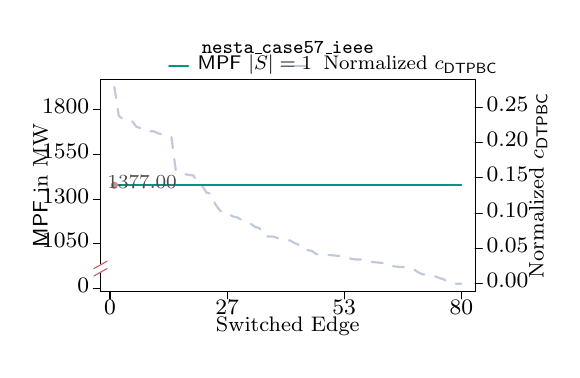
\begin{tikzpicture}[x=1pt,y=1pt]
\definecolor{fillColor}{RGB}{255,255,255}
\path[use as bounding box,fill=fillColor,fill opacity=0.00] (0,0) rectangle (440.85,271.01);
\begin{scope}
\path[clip] (  0.00,  0.00) rectangle (440.85,271.01);
\definecolor{drawColor}{RGB}{193,202,220}

\path[draw=drawColor,line width= 0.8pt,dash pattern=on 4pt off 4pt ,line join=round,line cap=round] ( 72.86,221.20) --
	( 76.55,196.85) --
	( 80.24,194.07) --
	( 83.93,192.58) --
	( 87.62,192.58) --
	( 91.31,187.75) --
	( 95.00,186.63) --
	( 98.69,184.03) --
	(102.38,184.03) --
	(106.07,183.85) --
	(109.76,182.17) --
	(113.45,181.25) --
	(117.14,179.57) --
	(120.83,179.02) --
	(124.52,150.58) --
	(128.21,148.73) --
	(131.90,147.98) --
	(135.59,147.24) --
	(139.28,146.87) --
	(142.97,140.55) --
	(146.66,137.95) --
	(150.35,132.37) --
	(154.05,131.63) --
	(157.74,122.53) --
	(161.43,117.51) --
	(165.12,114.54) --
	(168.81,114.54) --
	(172.50,112.31) --
	(176.19,111.56) --
	(179.88,109.33) --
	(183.57,107.85) --
	(187.26,106.36) --
	(190.95,103.57) --
	(194.64,102.64) --
	(198.33, 95.95) --
	(202.02, 95.58) --
	(205.71, 95.58) --
	(209.40, 94.47) --
	(213.09, 92.98) --
	(216.78, 92.24) --
	(220.47, 92.24) --
	(224.16, 90.01) --
	(227.85, 88.52) --
	(231.54, 88.52) --
	(235.23, 84.06) --
	(238.92, 83.32) --
	(242.61, 80.72) --
	(246.30, 80.34) --
	(249.99, 80.16) --
	(253.68, 79.97) --
	(257.37, 79.60) --
	(261.06, 79.23) --
	(264.75, 78.86) --
	(268.44, 78.49) --
	(272.13, 76.63) --
	(275.82, 76.26) --
	(279.51, 76.26) --
	(283.20, 75.88) --
	(286.89, 74.40) --
	(290.58, 74.03) --
	(294.27, 73.65) --
	(297.96, 73.28) --
	(301.65, 71.05) --
	(305.34, 70.68) --
	(309.03, 70.31) --
	(312.72, 69.94) --
	(316.41, 69.94) --
	(320.10, 69.19) --
	(323.79, 68.64) --
	(327.48, 65.85) --
	(331.17, 63.99) --
	(334.86, 63.25) --
	(338.55, 62.50) --
	(342.24, 62.13) --
	(345.94, 60.65) --
	(349.63, 59.53) --
	(353.32, 56.93) --
	(357.01, 56.19) --
	(360.70, 55.82) --
	(364.39, 55.82);
\end{scope}
\begin{scope}
\path[clip] (  0.00,  0.00) rectangle (440.85,271.01);
\definecolor{drawColor}{RGB}{0,0,0}

\path[draw=drawColor,line width= 0.4pt,line join=round,line cap=round] ( 61.20, 49.20) --
	(376.05, 49.20) --
	(376.05,227.81) --
	( 61.20,227.81) --
	( 61.20, 49.20);
\end{scope}
\begin{scope}
\path[clip] (  0.00,  0.00) rectangle (440.85,271.01);
\definecolor{drawColor}{RGB}{0,0,0}

\path[draw=drawColor,line width= 0.4pt,line join=round,line cap=round] (376.05, 55.82) -- (376.05,204.10);

\path[draw=drawColor,line width= 0.4pt,line join=round,line cap=round] (376.05, 55.82) -- (382.05, 55.82);

\path[draw=drawColor,line width= 0.4pt,line join=round,line cap=round] (376.05, 85.47) -- (382.05, 85.47);

\path[draw=drawColor,line width= 0.4pt,line join=round,line cap=round] (376.05,115.13) -- (382.05,115.13);

\path[draw=drawColor,line width= 0.4pt,line join=round,line cap=round] (376.05,144.79) -- (382.05,144.79);

\path[draw=drawColor,line width= 0.4pt,line join=round,line cap=round] (376.05,174.44) -- (382.05,174.44);

\path[draw=drawColor,line width= 0.4pt,line join=round,line cap=round] (376.05,204.10) -- (382.05,204.10);

\node[text=drawColor,anchor=base west,inner sep=0pt, outer sep=0pt, scale=  1.00] at (385.65, 52.37) {0.00};

\node[text=drawColor,anchor=base west,inner sep=0pt, outer sep=0pt, scale=  1.00] at (385.65, 82.03) {0.05};

\node[text=drawColor,anchor=base west,inner sep=0pt, outer sep=0pt, scale=  1.00] at (385.65,111.69) {0.10};

\node[text=drawColor,anchor=base west,inner sep=0pt, outer sep=0pt, scale=  1.00] at (385.65,141.34) {0.15};

\node[text=drawColor,anchor=base west,inner sep=0pt, outer sep=0pt, scale=  1.00] at (385.65,171.00) {0.20};

\node[text=drawColor,anchor=base west,inner sep=0pt, outer sep=0pt, scale=  1.00] at (385.65,200.66) {0.25};
\end{scope}
\begin{scope}
\path[clip] (  0.00,  0.00) rectangle (440.85,271.01);
\definecolor{drawColor}{RGB}{0,150,130}

\path[draw=drawColor,line width= 0.8pt,line join=round,line cap=round] (118.89,238.60) -- (134.91,238.60);
\definecolor{drawColor}{RGB}{193,202,220}

\path[draw=drawColor,line width= 0.8pt,dash pattern=on 4pt off 4pt ,line join=round,line cap=round] (224.63,238.60) -- (240.65,238.60);
\definecolor{drawColor}{RGB}{0,0,0}

\node[text=drawColor,anchor=base,inner sep=0pt, outer sep=0pt, scale=  0.89] at (218.62,249.28) {\texttt{nesta\_case57\_ieee}};

\node[text=drawColor,anchor=base west,inner sep=0pt, outer sep=0pt, scale=  0.89] at (142.92,235.54) {$\mathsf{MPF}~|S|=1$};

\node[text=drawColor,anchor=base west,inner sep=0pt, outer sep=0pt, scale=  0.89] at (248.66,235.54) {Normalized~$c_\mathsf{DTPBC}$};
\end{scope}
\begin{scope}
\path[clip] (  0.00,  0.00) rectangle (440.85,271.01);
\definecolor{drawColor}{RGB}{0,0,0}

\path[draw=drawColor,line width= 0.4pt,line join=round,line cap=round] ( 61.20, 51.88) -- ( 61.20,202.01);

\path[draw=drawColor,line width= 0.4pt,line join=round,line cap=round] ( 61.20, 51.88) -- ( 55.20, 51.88);

\path[draw=drawColor,line width= 0.4pt,line join=round,line cap=round] ( 61.20, 89.41) -- ( 55.20, 89.41);

\path[draw=drawColor,line width= 0.4pt,line join=round,line cap=round] ( 61.20,126.95) -- ( 55.20,126.95);

\path[draw=drawColor,line width= 0.4pt,line join=round,line cap=round] ( 61.20,164.48) -- ( 55.20,164.48);

\path[draw=drawColor,line width= 0.4pt,line join=round,line cap=round] ( 61.20,202.01) -- ( 55.20,202.01);

\node[text=drawColor,anchor=base east,inner sep=0pt, outer sep=0pt, scale=  1.00] at ( 51.60, 48.44) {0};

\node[text=drawColor,anchor=base east,inner sep=0pt, outer sep=0pt, scale=  1.00] at ( 51.60, 85.97) {1050};

\node[text=drawColor,anchor=base east,inner sep=0pt, outer sep=0pt, scale=  1.00] at ( 51.60,123.50) {1300};

\node[text=drawColor,anchor=base east,inner sep=0pt, outer sep=0pt, scale=  1.00] at ( 51.60,161.03) {1550};

\node[text=drawColor,anchor=base east,inner sep=0pt, outer sep=0pt, scale=  1.00] at ( 51.60,198.57) {1800};
\end{scope}
\begin{scope}
\path[clip] (  0.00,  0.00) rectangle (440.85,271.01);
\definecolor{drawColor}{RGB}{255,255,255}
\definecolor{fillColor}{RGB}{255,255,255}

\path[draw=drawColor,line width= 0.4pt,line join=round,line cap=round,fill=fillColor] ( 55.69, 65.44) rectangle ( 66.71, 71.69);
\definecolor{drawColor}{RGB}{188,97,104}

\path[draw=drawColor,line width= 0.4pt,line join=round,line cap=round] ( 55.69, 62.31) -- ( 66.71, 68.56);

\path[draw=drawColor,line width= 0.4pt,line join=round,line cap=round] ( 55.69, 68.56) -- ( 66.71, 74.81);
\end{scope}
\begin{scope}
\path[clip] ( 61.20, 49.20) rectangle (376.05,227.81);
\definecolor{drawColor}{RGB}{0,150,130}

\path[draw=drawColor,line width= 0.8pt,line join=round,line cap=round] ( 72.86,138.51) --
	( 76.55,138.51) --
	( 80.24,138.51) --
	( 83.93,138.51) --
	( 87.62,138.51) --
	( 91.31,138.51) --
	( 95.00,138.51) --
	( 98.69,138.51) --
	(102.38,138.51) --
	(106.07,138.51) --
	(109.76,138.51) --
	(113.45,138.51) --
	(117.14,138.51) --
	(120.83,138.51) --
	(124.52,138.51) --
	(128.21,138.51) --
	(131.90,138.51) --
	(135.59,138.51) --
	(139.28,138.51) --
	(142.97,138.51) --
	(146.66,138.51) --
	(150.35,138.51) --
	(154.05,138.51) --
	(157.74,138.51) --
	(161.43,138.51) --
	(165.12,138.51) --
	(168.81,138.51) --
	(172.50,138.51) --
	(176.19,138.51) --
	(179.88,138.51) --
	(183.57,138.51) --
	(187.26,138.51) --
	(190.95,138.51) --
	(194.64,138.51) --
	(198.33,138.51) --
	(202.02,138.51) --
	(205.71,138.51) --
	(209.40,138.51) --
	(213.09,138.51) --
	(216.78,138.51) --
	(220.47,138.51) --
	(224.16,138.51) --
	(227.85,138.51) --
	(231.54,138.51) --
	(235.23,138.51) --
	(238.92,138.51) --
	(242.61,138.51) --
	(246.30,138.51) --
	(249.99,138.51) --
	(253.68,138.51) --
	(257.37,138.51) --
	(261.06,138.51) --
	(264.75,138.51) --
	(268.44,138.51) --
	(272.13,138.51) --
	(275.82,138.51) --
	(279.51,138.51) --
	(283.20,138.51) --
	(286.89,138.51) --
	(290.58,138.51) --
	(294.27,138.51) --
	(297.96,138.51) --
	(301.65,138.51) --
	(305.34,138.51) --
	(309.03,138.51) --
	(312.72,138.51) --
	(316.41,138.51) --
	(320.10,138.51) --
	(323.79,138.51) --
	(327.48,138.51) --
	(331.17,138.51) --
	(334.86,138.51) --
	(338.55,138.51) --
	(342.24,138.51) --
	(345.94,138.51) --
	(349.63,138.51) --
	(353.32,138.51) --
	(357.01,138.51) --
	(360.70,138.51) --
	(364.39,138.51);
\end{scope}
\begin{scope}
\path[clip] ( 61.20, 49.20) rectangle (376.05,227.81);
\definecolor{fillColor}{RGB}{207,142,147}

\path[fill=fillColor] ( 72.86,138.51) circle (  3.15);
\end{scope}
\begin{scope}
\path[clip] ( 61.20, 49.20) rectangle (376.05,227.81);
\definecolor{drawColor}{gray}{0.30}

\node[text=drawColor,anchor=base,inner sep=0pt, outer sep=0pt, scale=  0.90] at ( 96.18,135.62) {1377.00};
\end{scope}
\begin{scope}
\path[clip] (  0.00,  0.00) rectangle (440.85,271.01);
\definecolor{drawColor}{RGB}{0,0,0}

\path[draw=drawColor,line width= 0.4pt,line join=round,line cap=round] ( 69.17, 49.20) -- (364.39, 49.20);

\path[draw=drawColor,line width= 0.4pt,line join=round,line cap=round] ( 69.17, 49.20) -- ( 69.17, 43.20);

\path[draw=drawColor,line width= 0.4pt,line join=round,line cap=round] (167.58, 49.20) -- (167.58, 43.20);

\path[draw=drawColor,line width= 0.4pt,line join=round,line cap=round] (265.98, 49.20) -- (265.98, 43.20);

\path[draw=drawColor,line width= 0.4pt,line join=round,line cap=round] (364.39, 49.20) -- (364.39, 43.20);

\node[text=drawColor,anchor=base,inner sep=0pt, outer sep=0pt, scale=  1.00] at ( 69.17, 30.00) {0};

\node[text=drawColor,anchor=base,inner sep=0pt, outer sep=0pt, scale=  1.00] at (167.58, 30.00) {27};

\node[text=drawColor,anchor=base,inner sep=0pt, outer sep=0pt, scale=  1.00] at (265.98, 30.00) {53};

\node[text=drawColor,anchor=base,inner sep=0pt, outer sep=0pt, scale=  1.00] at (364.39, 30.00) {80};

\node[text=drawColor,anchor=base,inner sep=0pt, outer sep=0pt, scale=  0.95] at (218.62, 15.60) {Switched Edge};

\node[text=drawColor,rotate= 90.00,anchor=base,inner sep=0pt, outer sep=0pt, scale=  0.95] at ( 16.80,138.51) {$\mathsf{MPF}$ in~$\mathrm{MW}$};

\node[text=drawColor,rotate= 90.00,anchor=base,inner sep=0pt, outer sep=0pt, scale=  0.95] at (433.65,138.51) {Normalized~$c_\mathsf{DTPBC}$};
\end{scope}
\end{tikzpicture}
%
    \label{plot:SwitchingBetweenness_nesta_case57_ieee_dtpbc_mpf_cutY}%
  \end{subfigure}%
  \hfill
  %
  \begin{subfigure}[t]{.5\textwidth}%
    \centering%
    % Created by tikzDevice version 0.10.1 on 2018-01-31 10:28:46
% !TEX encoding = UTF-8 Unicode
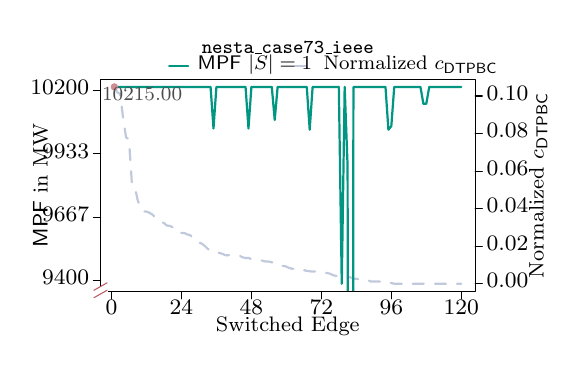
\begin{tikzpicture}[x=1pt,y=1pt]
\definecolor{fillColor}{RGB}{255,255,255}
\path[use as bounding box,fill=fillColor,fill opacity=0.00] (0,0) rectangle (440.85,271.01);
\begin{scope}
\path[clip] (  0.00,  0.00) rectangle (440.85,271.01);
\definecolor{drawColor}{RGB}{193,202,220}

\path[draw=drawColor,line width= 0.8pt,dash pattern=on 4pt off 4pt ,line join=round,line cap=round] ( 72.86,221.20) --
	( 75.31,216.69) --
	( 77.76,215.19) --
	( 80.21,194.78) --
	( 82.66,178.88) --
	( 85.11,177.07) --
	( 87.56,140.46) --
	( 90.01,137.46) --
	( 92.46,126.05) --
	( 94.91,119.45) --
	( 97.36,116.45) --
	( 99.81,116.45) --
	(102.26,115.54) --
	(104.71,114.04) --
	(107.16,111.64) --
	(109.61,110.44) --
	(112.06,107.74) --
	(114.51,106.84) --
	(116.96,104.74) --
	(119.41,104.44) --
	(121.86,103.24) --
	(124.31,103.24) --
	(126.76,100.24) --
	(129.21, 98.44) --
	(131.66, 98.44) --
	(134.11, 97.24) --
	(136.56, 96.64) --
	(139.01, 94.23) --
	(141.46, 91.23) --
	(143.90, 90.63) --
	(146.35, 89.43) --
	(148.80, 87.63) --
	(151.25, 85.23) --
	(153.70, 83.43) --
	(156.15, 83.43) --
	(158.60, 83.43) --
	(161.05, 81.63) --
	(163.50, 81.03) --
	(165.95, 79.83) --
	(168.40, 79.83) --
	(170.85, 79.83) --
	(173.30, 79.23) --
	(175.75, 79.23) --
	(178.20, 79.23) --
	(180.65, 78.03) --
	(183.10, 77.43) --
	(185.55, 77.43) --
	(188.00, 76.53) --
	(190.45, 76.23) --
	(192.90, 75.63) --
	(195.35, 75.63) --
	(197.80, 75.02) --
	(200.25, 74.42) --
	(202.70, 74.42) --
	(205.15, 73.82) --
	(207.60, 73.22) --
	(210.05, 71.42) --
	(212.50, 70.82) --
	(214.95, 70.82) --
	(217.40, 70.22) --
	(219.85, 69.02) --
	(222.30, 68.42) --
	(224.75, 68.42) --
	(227.20, 67.82) --
	(229.65, 67.82) --
	(232.10, 67.22) --
	(234.55, 66.62) --
	(237.00, 66.32) --
	(239.45, 66.02) --
	(241.90, 66.02) --
	(244.35, 65.42) --
	(246.80, 65.12) --
	(249.25, 64.82) --
	(251.70, 64.82) --
	(254.15, 64.22) --
	(256.60, 63.02) --
	(259.05, 62.42) --
	(261.49, 62.42) --
	(263.94, 61.82) --
	(266.39, 61.82) --
	(268.84, 61.22) --
	(271.29, 61.22) --
	(273.74, 60.02) --
	(276.19, 60.02) --
	(278.64, 59.42) --
	(281.09, 59.42) --
	(283.54, 59.42) --
	(285.99, 58.82) --
	(288.44, 57.62) --
	(290.89, 57.62) --
	(293.34, 57.62) --
	(295.79, 57.62) --
	(298.24, 57.62) --
	(300.69, 57.02) --
	(303.14, 56.42) --
	(305.59, 56.42) --
	(308.04, 55.82) --
	(310.49, 55.82) --
	(312.94, 55.82) --
	(315.39, 55.82) --
	(317.84, 55.82) --
	(320.29, 55.82) --
	(322.74, 55.82) --
	(325.19, 55.82) --
	(327.64, 55.82) --
	(330.09, 55.82) --
	(332.54, 55.82) --
	(334.99, 55.82) --
	(337.44, 55.82) --
	(339.89, 55.82) --
	(342.34, 55.82) --
	(344.79, 55.82) --
	(347.24, 55.82) --
	(349.69, 55.82) --
	(352.14, 55.82) --
	(354.59, 55.82) --
	(357.04, 55.82) --
	(359.49, 55.82) --
	(361.94, 55.82) --
	(364.39, 55.82);
\end{scope}
\begin{scope}
\path[clip] (  0.00,  0.00) rectangle (440.85,271.01);
\definecolor{drawColor}{RGB}{0,0,0}

\path[draw=drawColor,line width= 0.4pt,line join=round,line cap=round] ( 61.20, 49.20) --
	(376.05, 49.20) --
	(376.05,227.81) --
	( 61.20,227.81) --
	( 61.20, 49.20);
\end{scope}
\begin{scope}
\path[clip] (  0.00,  0.00) rectangle (440.85,271.01);
\definecolor{drawColor}{RGB}{0,0,0}

\path[draw=drawColor,line width= 0.4pt,line join=round,line cap=round] (376.05, 55.82) -- (376.05,213.57);

\path[draw=drawColor,line width= 0.4pt,line join=round,line cap=round] (376.05, 55.82) -- (382.05, 55.82);

\path[draw=drawColor,line width= 0.4pt,line join=round,line cap=round] (376.05, 87.37) -- (382.05, 87.37);

\path[draw=drawColor,line width= 0.4pt,line join=round,line cap=round] (376.05,118.92) -- (382.05,118.92);

\path[draw=drawColor,line width= 0.4pt,line join=round,line cap=round] (376.05,150.47) -- (382.05,150.47);

\path[draw=drawColor,line width= 0.4pt,line join=round,line cap=round] (376.05,182.02) -- (382.05,182.02);

\path[draw=drawColor,line width= 0.4pt,line join=round,line cap=round] (376.05,213.57) -- (382.05,213.57);

\node[text=drawColor,anchor=base west,inner sep=0pt, outer sep=0pt, scale=  1.00] at (385.65, 52.37) {0.00};

\node[text=drawColor,anchor=base west,inner sep=0pt, outer sep=0pt, scale=  1.00] at (385.65, 83.92) {0.02};

\node[text=drawColor,anchor=base west,inner sep=0pt, outer sep=0pt, scale=  1.00] at (385.65,115.47) {0.04};

\node[text=drawColor,anchor=base west,inner sep=0pt, outer sep=0pt, scale=  1.00] at (385.65,147.03) {0.06};

\node[text=drawColor,anchor=base west,inner sep=0pt, outer sep=0pt, scale=  1.00] at (385.65,178.58) {0.08};

\node[text=drawColor,anchor=base west,inner sep=0pt, outer sep=0pt, scale=  1.00] at (385.65,210.13) {0.10};
\end{scope}
\begin{scope}
\path[clip] (  0.00,  0.00) rectangle (440.85,271.01);
\definecolor{drawColor}{RGB}{0,150,130}

\path[draw=drawColor,line width= 0.8pt,line join=round,line cap=round] (118.89,238.60) -- (134.91,238.60);
\definecolor{drawColor}{RGB}{193,202,220}

\path[draw=drawColor,line width= 0.8pt,dash pattern=on 4pt off 4pt ,line join=round,line cap=round] (224.63,238.60) -- (240.65,238.60);
\definecolor{drawColor}{RGB}{0,0,0}

\node[text=drawColor,anchor=base,inner sep=0pt, outer sep=0pt, scale=  0.89] at (218.62,249.28) {\texttt{nesta\_case73\_ieee}};

\node[text=drawColor,anchor=base west,inner sep=0pt, outer sep=0pt, scale=  0.89] at (142.92,235.54) {$\mathsf{MPF}~|S|=1$};

\node[text=drawColor,anchor=base west,inner sep=0pt, outer sep=0pt, scale=  0.89] at (248.66,235.54) {Normalized~$c_\mathsf{DTPBC}$};
\end{scope}
\begin{scope}
\path[clip] (  0.00,  0.00) rectangle (440.85,271.01);
\definecolor{drawColor}{RGB}{0,0,0}

\path[draw=drawColor,line width= 0.4pt,line join=round,line cap=round] ( 61.20, 58.32) -- ( 61.20,218.20);

\path[draw=drawColor,line width= 0.4pt,line join=round,line cap=round] ( 61.20, 58.32) -- ( 55.20, 58.32);

\path[draw=drawColor,line width= 0.4pt,line join=round,line cap=round] ( 61.20,111.61) -- ( 55.20,111.61);

\path[draw=drawColor,line width= 0.4pt,line join=round,line cap=round] ( 61.20,164.91) -- ( 55.20,164.91);

\path[draw=drawColor,line width= 0.4pt,line join=round,line cap=round] ( 61.20,218.20) -- ( 55.20,218.20);

\node[text=drawColor,anchor=base east,inner sep=0pt, outer sep=0pt, scale=  1.00] at ( 51.60, 54.88) {9400};

\node[text=drawColor,anchor=base east,inner sep=0pt, outer sep=0pt, scale=  1.00] at ( 51.60,108.17) {9667};

\node[text=drawColor,anchor=base east,inner sep=0pt, outer sep=0pt, scale=  1.00] at ( 51.60,161.46) {9933};

\node[text=drawColor,anchor=base east,inner sep=0pt, outer sep=0pt, scale=  1.00] at ( 51.60,214.76) {10200};
\end{scope}
\begin{scope}
\path[clip] (  0.00,  0.00) rectangle (440.85,271.01);
\definecolor{drawColor}{RGB}{255,255,255}
\definecolor{fillColor}{RGB}{255,255,255}

\path[draw=drawColor,line width= 0.4pt,line join=round,line cap=round,fill=fillColor] ( 55.69, 47.20) rectangle ( 66.71, 53.45);
\definecolor{drawColor}{RGB}{188,97,104}

\path[draw=drawColor,line width= 0.4pt,line join=round,line cap=round] ( 55.69, 44.08) -- ( 66.71, 50.33);

\path[draw=drawColor,line width= 0.4pt,line join=round,line cap=round] ( 55.69, 50.33) -- ( 66.71, 56.58);
\end{scope}
\begin{scope}
\path[clip] ( 61.20, 49.20) rectangle (376.05,227.81);
\definecolor{drawColor}{RGB}{0,150,130}

\path[draw=drawColor,line width= 0.8pt,line join=round,line cap=round] ( 72.86,221.20) --
	( 75.31,221.20) --
	( 77.76,221.20) --
	( 80.21,221.20) --
	( 82.66,221.20) --
	( 85.11,221.20) --
	( 87.56,221.20) --
	( 90.01,221.20) --
	( 92.46,221.20) --
	( 94.91,221.20) --
	( 97.36,221.20) --
	( 99.81,221.20) --
	(102.26,221.20) --
	(104.71,221.20) --
	(107.16,221.20) --
	(109.61,221.20) --
	(112.06,221.20) --
	(114.51,221.20) --
	(116.96,221.20) --
	(119.41,221.20) --
	(121.86,221.20) --
	(124.31,221.20) --
	(126.76,221.20) --
	(129.21,221.20) --
	(131.66,221.20) --
	(134.11,221.20) --
	(136.56,221.20) --
	(139.01,221.20) --
	(141.46,221.20) --
	(143.90,221.20) --
	(146.35,221.20) --
	(148.80,221.20) --
	(151.25,221.20) --
	(153.70,221.20) --
	(156.15,186.22) --
	(158.60,221.20) --
	(161.05,221.20) --
	(163.50,221.20) --
	(165.95,221.20) --
	(168.40,221.20) --
	(170.85,221.20) --
	(173.30,221.20) --
	(175.75,221.20) --
	(178.20,221.20) --
	(180.65,221.20) --
	(183.10,221.20) --
	(185.55,186.22) --
	(188.00,221.20) --
	(190.45,221.20) --
	(192.90,221.20) --
	(195.35,221.20) --
	(197.80,221.20) --
	(200.25,221.20) --
	(202.70,221.20) --
	(205.15,221.20) --
	(207.60,193.44) --
	(210.05,221.20) --
	(212.50,221.20) --
	(214.95,221.20) --
	(217.40,221.20) --
	(219.85,221.20) --
	(222.30,221.20) --
	(224.75,221.20) --
	(227.20,221.20) --
	(229.65,221.20) --
	(232.10,221.20) --
	(234.55,221.20) --
	(237.00,185.26) --
	(239.45,221.20) --
	(241.90,221.20) --
	(244.35,221.20) --
	(246.80,221.20) --
	(249.25,221.20) --
	(251.70,221.20) --
	(254.15,221.20) --
	(256.60,221.20) --
	(259.05,221.20) --
	(261.49,221.20) --
	(263.94, 55.82) --
	(266.39,221.20) --
	(268.84,154.73) --
	(269.04,  0.00);

\path[draw=drawColor,line width= 0.8pt,line join=round,line cap=round] (273.48,  0.00) --
	(273.74,221.20) --
	(276.19,221.20) --
	(278.64,221.20) --
	(281.09,221.20) --
	(283.54,221.20) --
	(285.99,221.20) --
	(288.44,221.20) --
	(290.89,221.20) --
	(293.34,221.20) --
	(295.79,221.20) --
	(298.24,221.20) --
	(300.69,221.20) --
	(303.14,185.26) --
	(305.59,188.24) --
	(308.04,221.20) --
	(310.49,221.20) --
	(312.94,221.20) --
	(315.39,221.20) --
	(317.84,221.20) --
	(320.29,221.20) --
	(322.74,221.20) --
	(325.19,221.20) --
	(327.64,221.20) --
	(330.09,221.20) --
	(332.54,207.05) --
	(334.99,207.05) --
	(337.44,221.20) --
	(339.89,221.20) --
	(342.34,221.20) --
	(344.79,221.20) --
	(347.24,221.20) --
	(349.69,221.20) --
	(352.14,221.20) --
	(354.59,221.20) --
	(357.04,221.20) --
	(359.49,221.20) --
	(361.94,221.20) --
	(364.39,221.20);
\end{scope}
\begin{scope}
\path[clip] ( 61.20, 49.20) rectangle (376.05,227.81);
\definecolor{fillColor}{RGB}{207,142,147}

\path[fill=fillColor] ( 72.86,221.20) circle (  3.15);
\end{scope}
\begin{scope}
\path[clip] ( 61.20, 49.20) rectangle (376.05,227.81);
\definecolor{drawColor}{gray}{0.30}

\node[text=drawColor,anchor=base,inner sep=0pt, outer sep=0pt, scale=  0.90] at ( 96.18,210.04) {10215.00};
\end{scope}
\begin{scope}
\path[clip] (  0.00,  0.00) rectangle (440.85,271.01);
\definecolor{drawColor}{RGB}{0,0,0}

\path[draw=drawColor,line width= 0.4pt,line join=round,line cap=round] ( 70.41, 49.20) -- (364.39, 49.20);

\path[draw=drawColor,line width= 0.4pt,line join=round,line cap=round] ( 70.41, 49.20) -- ( 70.41, 43.20);

\path[draw=drawColor,line width= 0.4pt,line join=round,line cap=round] (129.21, 49.20) -- (129.21, 43.20);

\path[draw=drawColor,line width= 0.4pt,line join=round,line cap=round] (188.00, 49.20) -- (188.00, 43.20);

\path[draw=drawColor,line width= 0.4pt,line join=round,line cap=round] (246.80, 49.20) -- (246.80, 43.20);

\path[draw=drawColor,line width= 0.4pt,line join=round,line cap=round] (305.59, 49.20) -- (305.59, 43.20);

\path[draw=drawColor,line width= 0.4pt,line join=round,line cap=round] (364.39, 49.20) -- (364.39, 43.20);

\node[text=drawColor,anchor=base,inner sep=0pt, outer sep=0pt, scale=  1.00] at ( 70.41, 30.00) {0};

\node[text=drawColor,anchor=base,inner sep=0pt, outer sep=0pt, scale=  1.00] at (129.21, 30.00) {24};

\node[text=drawColor,anchor=base,inner sep=0pt, outer sep=0pt, scale=  1.00] at (188.00, 30.00) {48};

\node[text=drawColor,anchor=base,inner sep=0pt, outer sep=0pt, scale=  1.00] at (246.80, 30.00) {72};

\node[text=drawColor,anchor=base,inner sep=0pt, outer sep=0pt, scale=  1.00] at (305.59, 30.00) {96};

\node[text=drawColor,anchor=base,inner sep=0pt, outer sep=0pt, scale=  1.00] at (364.39, 30.00) {120};

\node[text=drawColor,anchor=base,inner sep=0pt, outer sep=0pt, scale=  0.95] at (218.62, 15.60) {Switched Edge};

\node[text=drawColor,rotate= 90.00,anchor=base,inner sep=0pt, outer sep=0pt, scale=  0.95] at ( 16.80,138.51) {$\mathsf{MPF}$ in~$\mathrm{MW}$};

\node[text=drawColor,rotate= 90.00,anchor=base,inner sep=0pt, outer sep=0pt, scale=  0.95] at (433.65,138.51) {Normalized~$c_\mathsf{DTPBC}$};
\end{scope}
\end{tikzpicture}
%
    \label{plot:SwitchingBetweenness_nesta_case73_ieee_rts_dtpbc_mpf_cutY}%
  \end{subfigure}%

  %
  \begin{subfigure}[t]{.5\textwidth}%
    \centering%
    % Created by tikzDevice version 0.10.1 on 2018-01-31 10:28:54
% !TEX encoding = UTF-8 Unicode
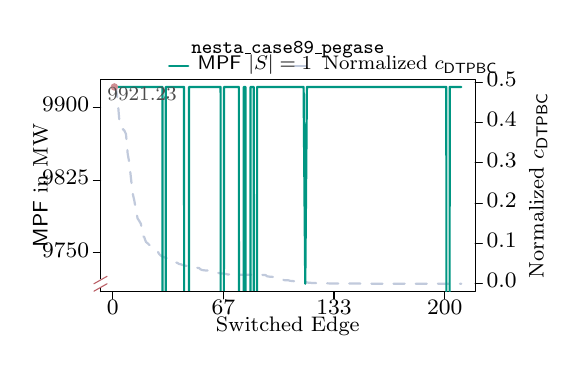
\begin{tikzpicture}[x=1pt,y=1pt]
\definecolor{fillColor}{RGB}{255,255,255}
\path[use as bounding box,fill=fillColor,fill opacity=0.00] (0,0) rectangle (440.85,271.01);
\begin{scope}
\path[clip] (  0.00,  0.00) rectangle (440.85,271.01);
\definecolor{drawColor}{RGB}{193,202,220}

\path[draw=drawColor,line width= 0.8pt,dash pattern=on 4pt off 4pt ,line join=round,line cap=round] ( 72.86,221.20) --
	( 74.26,220.12) --
	( 75.65,209.79) --
	( 77.05,192.73) --
	( 78.44,186.68) --
	( 79.84,185.86) --
	( 81.23,184.60) --
	( 82.62,181.58) --
	( 84.02,165.25) --
	( 85.41,157.39) --
	( 86.81,144.42) --
	( 88.20,131.90) --
	( 89.60,125.76) --
	( 90.99,117.47) --
	( 92.39,110.68) --
	( 93.78,108.57) --
	( 95.18,106.06) --
	( 96.57, 96.25) --
	( 97.97, 94.96) --
	( 99.36, 90.98) --
	(100.76, 89.86) --
	(102.15, 88.52) --
	(103.55, 87.22) --
	(104.94, 86.71) --
	(106.34, 85.76) --
	(107.73, 84.42) --
	(109.13, 83.34) --
	(110.52, 80.70) --
	(111.92, 79.45) --
	(113.31, 78.67) --
	(114.71, 78.11) --
	(116.10, 77.55) --
	(117.50, 77.33) --
	(118.89, 76.86) --
	(120.29, 76.21) --
	(121.68, 75.78) --
	(123.08, 73.92) --
	(124.47, 73.74) --
	(125.87, 73.36) --
	(127.26, 72.36) --
	(128.66, 72.23) --
	(130.05, 71.50) --
	(131.44, 71.41) --
	(132.84, 70.85) --
	(134.23, 70.85) --
	(135.63, 69.90) --
	(137.02, 69.73) --
	(138.42, 69.60) --
	(139.81, 69.51) --
	(141.21, 69.21) --
	(142.60, 69.17) --
	(144.00, 69.04) --
	(145.39, 67.83) --
	(146.79, 67.31) --
	(148.18, 67.13) --
	(149.58, 66.96) --
	(150.97, 66.92) --
	(152.37, 66.62) --
	(153.76, 66.36) --
	(155.16, 66.31) --
	(156.55, 65.32) --
	(157.95, 65.15) --
	(159.34, 64.97) --
	(160.74, 64.80) --
	(162.13, 64.50) --
	(163.53, 64.46) --
	(164.92, 64.20) --
	(166.32, 64.11) --
	(167.71, 63.68) --
	(169.11, 63.64) --
	(170.50, 63.46) --
	(171.90, 63.42) --
	(173.29, 63.42) --
	(174.69, 63.42) --
	(176.08, 63.42) --
	(177.48, 63.42) --
	(178.87, 63.42) --
	(180.26, 63.42) --
	(181.66, 63.42) --
	(183.05, 63.42) --
	(184.45, 63.42) --
	(185.84, 63.42) --
	(187.24, 63.42) --
	(188.63, 63.42) --
	(190.03, 63.42) --
	(191.42, 63.42) --
	(192.82, 63.33) --
	(194.21, 63.33) --
	(195.61, 63.25) --
	(197.00, 63.20) --
	(198.40, 63.20) --
	(199.79, 63.16) --
	(201.19, 62.08) --
	(202.58, 61.86) --
	(203.98, 61.69) --
	(205.37, 61.65) --
	(206.77, 61.43) --
	(208.16, 61.26) --
	(209.56, 60.87) --
	(210.95, 60.83) --
	(212.35, 60.39) --
	(213.74, 60.31) --
	(215.14, 58.93) --
	(216.53, 58.71) --
	(217.93, 58.71) --
	(219.32, 58.67) --
	(220.72, 58.23) --
	(222.11, 58.19) --
	(223.51, 57.98) --
	(224.90, 57.85) --
	(226.30, 57.72) --
	(227.69, 57.59) --
	(229.08, 57.54) --
	(230.48, 57.50) --
	(231.87, 57.50) --
	(233.27, 57.20) --
	(234.66, 56.94) --
	(236.06, 56.68) --
	(237.45, 56.64) --
	(238.85, 56.46) --
	(240.24, 56.42) --
	(241.64, 56.38) --
	(243.03, 56.33) --
	(244.43, 56.33) --
	(245.82, 56.33) --
	(247.22, 56.25) --
	(248.61, 56.16) --
	(250.01, 56.16) --
	(251.40, 56.16) --
	(252.80, 56.12) --
	(254.19, 56.07) --
	(255.59, 56.07) --
	(256.98, 56.07) --
	(258.38, 56.07) --
	(259.77, 55.99) --
	(261.17, 55.99) --
	(262.56, 55.99) --
	(263.96, 55.99) --
	(265.35, 55.99) --
	(266.75, 55.99) --
	(268.14, 55.99) --
	(269.54, 55.99) --
	(270.93, 55.99) --
	(272.33, 55.99) --
	(273.72, 55.99) --
	(275.12, 55.99) --
	(276.51, 55.99) --
	(277.90, 55.94) --
	(279.30, 55.94) --
	(280.69, 55.94) --
	(282.09, 55.90) --
	(283.48, 55.90) --
	(284.88, 55.90) --
	(286.27, 55.90) --
	(287.67, 55.90) --
	(289.06, 55.90) --
	(290.46, 55.90) --
	(291.85, 55.90) --
	(293.25, 55.90) --
	(294.64, 55.90) --
	(296.04, 55.86) --
	(297.43, 55.82) --
	(298.83, 55.82) --
	(300.22, 55.82) --
	(301.62, 55.82) --
	(303.01, 55.82) --
	(304.41, 55.82) --
	(305.80, 55.82) --
	(307.20, 55.82) --
	(308.59, 55.82) --
	(309.99, 55.82) --
	(311.38, 55.82) --
	(312.78, 55.82) --
	(314.17, 55.82) --
	(315.57, 55.82) --
	(316.96, 55.82) --
	(318.36, 55.82) --
	(319.75, 55.82) --
	(321.15, 55.82) --
	(322.54, 55.82) --
	(323.94, 55.82) --
	(325.33, 55.82) --
	(326.72, 55.82) --
	(328.12, 55.82) --
	(329.51, 55.82) --
	(330.91, 55.82) --
	(332.30, 55.82) --
	(333.70, 55.82) --
	(335.09, 55.82) --
	(336.49, 55.82) --
	(337.88, 55.82) --
	(339.28, 55.82) --
	(340.67, 55.82) --
	(342.07, 55.82) --
	(343.46, 55.82) --
	(344.86, 55.82) --
	(346.25, 55.82) --
	(347.65, 55.82) --
	(349.04, 55.82) --
	(350.44, 55.82) --
	(351.83, 55.82) --
	(353.23, 55.82) --
	(354.62, 55.82) --
	(356.02, 55.82) --
	(357.41, 55.82) --
	(358.81, 55.82) --
	(360.20, 55.82) --
	(361.60, 55.82) --
	(362.99, 55.82) --
	(364.39, 55.82);
\end{scope}
\begin{scope}
\path[clip] (  0.00,  0.00) rectangle (440.85,271.01);
\definecolor{drawColor}{RGB}{0,0,0}

\path[draw=drawColor,line width= 0.4pt,line join=round,line cap=round] ( 61.20, 49.20) --
	(376.05, 49.20) --
	(376.05,227.81) --
	( 61.20,227.81) --
	( 61.20, 49.20);
\end{scope}
\begin{scope}
\path[clip] (  0.00,  0.00) rectangle (440.85,271.01);
\definecolor{drawColor}{RGB}{0,0,0}

\path[draw=drawColor,line width= 0.4pt,line join=round,line cap=round] (376.05, 55.82) -- (376.05,225.00);

\path[draw=drawColor,line width= 0.4pt,line join=round,line cap=round] (376.05, 55.82) -- (382.05, 55.82);

\path[draw=drawColor,line width= 0.4pt,line join=round,line cap=round] (376.05, 89.65) -- (382.05, 89.65);

\path[draw=drawColor,line width= 0.4pt,line join=round,line cap=round] (376.05,123.49) -- (382.05,123.49);

\path[draw=drawColor,line width= 0.4pt,line join=round,line cap=round] (376.05,157.33) -- (382.05,157.33);

\path[draw=drawColor,line width= 0.4pt,line join=round,line cap=round] (376.05,191.16) -- (382.05,191.16);

\path[draw=drawColor,line width= 0.4pt,line join=round,line cap=round] (376.05,225.00) -- (382.05,225.00);

\node[text=drawColor,anchor=base west,inner sep=0pt, outer sep=0pt, scale=  1.00] at (385.65, 52.37) {0.0};

\node[text=drawColor,anchor=base west,inner sep=0pt, outer sep=0pt, scale=  1.00] at (385.65, 86.21) {0.1};

\node[text=drawColor,anchor=base west,inner sep=0pt, outer sep=0pt, scale=  1.00] at (385.65,120.05) {0.2};

\node[text=drawColor,anchor=base west,inner sep=0pt, outer sep=0pt, scale=  1.00] at (385.65,153.88) {0.3};

\node[text=drawColor,anchor=base west,inner sep=0pt, outer sep=0pt, scale=  1.00] at (385.65,187.72) {0.4};

\node[text=drawColor,anchor=base west,inner sep=0pt, outer sep=0pt, scale=  1.00] at (385.65,221.56) {0.5};
\end{scope}
\begin{scope}
\path[clip] (  0.00,  0.00) rectangle (440.85,271.01);
\definecolor{drawColor}{RGB}{0,150,130}

\path[draw=drawColor,line width= 0.8pt,line join=round,line cap=round] (118.89,238.60) -- (134.91,238.60);
\definecolor{drawColor}{RGB}{193,202,220}

\path[draw=drawColor,line width= 0.8pt,dash pattern=on 4pt off 4pt ,line join=round,line cap=round] (224.63,238.60) -- (240.65,238.60);
\definecolor{drawColor}{RGB}{0,0,0}

\node[text=drawColor,anchor=base,inner sep=0pt, outer sep=0pt, scale=  0.89] at (218.62,249.28) {\texttt{nesta\_case89\_pegase}};

\node[text=drawColor,anchor=base west,inner sep=0pt, outer sep=0pt, scale=  0.89] at (142.92,235.54) {$\mathsf{MPF}~|S|=1$};

\node[text=drawColor,anchor=base west,inner sep=0pt, outer sep=0pt, scale=  0.89] at (248.66,235.54) {Normalized~$c_\mathsf{DTPBC}$};
\end{scope}
\begin{scope}
\path[clip] (  0.00,  0.00) rectangle (440.85,271.01);
\definecolor{drawColor}{RGB}{0,0,0}

\path[draw=drawColor,line width= 0.4pt,line join=round,line cap=round] ( 61.20, 81.70) -- ( 61.20,203.90);

\path[draw=drawColor,line width= 0.4pt,line join=round,line cap=round] ( 61.20, 81.70) -- ( 55.20, 81.70);

\path[draw=drawColor,line width= 0.4pt,line join=round,line cap=round] ( 61.20,142.80) -- ( 55.20,142.80);

\path[draw=drawColor,line width= 0.4pt,line join=round,line cap=round] ( 61.20,203.90) -- ( 55.20,203.90);

\node[text=drawColor,anchor=base east,inner sep=0pt, outer sep=0pt, scale=  1.00] at ( 51.60, 78.25) {9750};

\node[text=drawColor,anchor=base east,inner sep=0pt, outer sep=0pt, scale=  1.00] at ( 51.60,139.36) {9825};

\node[text=drawColor,anchor=base east,inner sep=0pt, outer sep=0pt, scale=  1.00] at ( 51.60,200.46) {9900};
\end{scope}
\begin{scope}
\path[clip] (  0.00,  0.00) rectangle (440.85,271.01);
\definecolor{drawColor}{RGB}{255,255,255}
\definecolor{fillColor}{RGB}{255,255,255}

\path[draw=drawColor,line width= 0.4pt,line join=round,line cap=round,fill=fillColor] ( 55.69, 52.69) rectangle ( 66.71, 58.94);
\definecolor{drawColor}{RGB}{188,97,104}

\path[draw=drawColor,line width= 0.4pt,line join=round,line cap=round] ( 55.69, 49.56) -- ( 66.71, 55.82);

\path[draw=drawColor,line width= 0.4pt,line join=round,line cap=round] ( 55.69, 55.82) -- ( 66.71, 62.07);
\end{scope}
\begin{scope}
\path[clip] ( 61.20, 49.20) rectangle (376.05,227.81);
\definecolor{drawColor}{RGB}{0,150,130}

\path[draw=drawColor,line width= 0.8pt,line join=round,line cap=round] ( 72.86,221.20) --
	( 74.26,221.20) --
	( 75.65,221.20) --
	( 77.05,221.20) --
	( 78.44,221.20) --
	( 79.84,221.20) --
	( 81.23,221.20) --
	( 82.62,221.20) --
	( 84.02,221.20) --
	( 85.41,221.20) --
	( 86.81,221.20) --
	( 88.20,221.20) --
	( 89.60,221.20) --
	( 90.99,221.20) --
	( 92.39,221.20) --
	( 93.78,221.20) --
	( 95.18,221.20) --
	( 96.57,221.20) --
	( 97.97,221.20) --
	( 99.36,221.20) --
	(100.76,221.20) --
	(102.15,221.20) --
	(103.55,221.20) --
	(104.94,221.20) --
	(106.34,221.20) --
	(107.73,221.20) --
	(109.13,221.20) --
	(110.52,221.20) --
	(111.92,221.20) --
	(113.31,221.20) --
	(113.35,  0.00);

\path[draw=drawColor,line width= 0.8pt,line join=round,line cap=round] (116.06,  0.00) --
	(116.10,221.20) --
	(117.50,221.20) --
	(118.89,221.20) --
	(120.29,221.20) --
	(121.68,221.20) --
	(123.08,221.20) --
	(124.47,221.20) --
	(125.87,221.20) --
	(127.26,221.20) --
	(128.66,221.20) --
	(130.05,221.20) --
	(131.44,221.20) --
	(131.48,  0.00);

\path[draw=drawColor,line width= 0.8pt,line join=round,line cap=round] (135.59,  0.00) --
	(135.63,221.20) --
	(137.02,221.20) --
	(138.42,221.20) --
	(139.81,221.20) --
	(141.21,221.20) --
	(142.60,221.20) --
	(144.00,221.20) --
	(145.39,221.20) --
	(146.79,221.20) --
	(148.18,221.20) --
	(149.58,221.20) --
	(150.97,221.20) --
	(152.37,221.20) --
	(153.76,221.20) --
	(155.16,221.20) --
	(156.55,221.20) --
	(157.95,221.20) --
	(159.34,221.20) --
	(160.74,221.20) --
	(162.13,221.20) --
	(162.17,  0.00);

\path[draw=drawColor,line width= 0.8pt,line join=round,line cap=round] (164.88,  0.00) --
	(164.92,221.20) --
	(166.32,221.20) --
	(167.71,221.20) --
	(169.11,221.20) --
	(170.50,221.20) --
	(171.90,221.20) --
	(173.29,221.20) --
	(174.69,221.20) --
	(176.08,221.20) --
	(177.48,221.20) --
	(177.51,  0.00);

\path[draw=drawColor,line width= 0.8pt,line join=round,line cap=round] (181.62,  0.00) --
	(181.66,221.20) --
	(183.05,221.20) --
	(183.09,  0.00);

\path[draw=drawColor,line width= 0.8pt,line join=round,line cap=round] (187.20,  0.00) --
	(187.24,221.20) --
	(188.63,221.20) --
	(190.03,221.20) --
	(190.07,  0.00);

\path[draw=drawColor,line width= 0.8pt,line join=round,line cap=round] (192.78,  0.00) --
	(192.82,221.20) --
	(194.21,221.20) --
	(195.61,221.20) --
	(197.00,221.20) --
	(198.40,221.20) --
	(199.79,221.20) --
	(201.19,221.20) --
	(202.58,221.20) --
	(203.98,221.20) --
	(205.37,221.20) --
	(206.77,221.20) --
	(208.16,221.20) --
	(209.56,221.20) --
	(210.95,221.20) --
	(212.35,221.20) --
	(213.74,221.20) --
	(215.14,221.20) --
	(216.53,221.20) --
	(217.93,221.20) --
	(219.32,221.20) --
	(220.72,221.20) --
	(222.11,221.20) --
	(223.51,221.20) --
	(224.90,221.20) --
	(226.30,221.20) --
	(227.69,221.20) --
	(229.08,221.20) --
	(230.48,221.20) --
	(231.87,221.20) --
	(233.27, 55.82) --
	(234.66,221.20) --
	(236.06,221.20) --
	(237.45,221.20) --
	(238.85,221.20) --
	(240.24,221.20) --
	(241.64,221.20) --
	(243.03,221.20) --
	(244.43,221.20) --
	(245.82,221.20) --
	(247.22,221.20) --
	(248.61,221.20) --
	(250.01,221.20) --
	(251.40,221.20) --
	(252.80,221.20) --
	(254.19,221.20) --
	(255.59,221.20) --
	(256.98,221.20) --
	(258.38,221.20) --
	(259.77,221.20) --
	(261.17,221.20) --
	(262.56,221.20) --
	(263.96,221.20) --
	(265.35,221.20) --
	(266.75,221.20) --
	(268.14,221.20) --
	(269.54,221.20) --
	(270.93,221.20) --
	(272.33,221.20) --
	(273.72,221.20) --
	(275.12,221.20) --
	(276.51,221.20) --
	(277.90,221.20) --
	(279.30,221.20) --
	(280.69,221.20) --
	(282.09,221.20) --
	(283.48,221.20) --
	(284.88,221.20) --
	(286.27,221.20) --
	(287.67,221.20) --
	(289.06,221.20) --
	(290.46,221.20) --
	(291.85,221.20) --
	(293.25,221.20) --
	(294.64,221.20) --
	(296.04,221.20) --
	(297.43,221.20) --
	(298.83,221.20) --
	(300.22,221.20) --
	(301.62,221.20) --
	(303.01,221.20) --
	(304.41,221.20) --
	(305.80,221.20) --
	(307.20,221.20) --
	(308.59,221.20) --
	(309.99,221.20) --
	(311.38,221.20) --
	(312.78,221.20) --
	(314.17,221.20) --
	(315.57,221.20) --
	(316.96,221.20) --
	(318.36,221.20) --
	(319.75,221.20) --
	(321.15,221.20) --
	(322.54,221.20) --
	(323.94,221.20) --
	(325.33,221.20) --
	(326.72,221.20) --
	(328.12,221.20) --
	(329.51,221.20) --
	(330.91,221.20) --
	(332.30,221.20) --
	(333.70,221.20) --
	(335.09,221.20) --
	(336.49,221.20) --
	(337.88,221.20) --
	(339.28,221.20) --
	(340.67,221.20) --
	(342.07,221.20) --
	(343.46,221.20) --
	(344.86,221.20) --
	(346.25,221.20) --
	(347.65,221.20) --
	(349.04,221.20) --
	(350.44,221.20) --
	(351.83,221.20) --
	(351.87,  0.00);

\path[draw=drawColor,line width= 0.8pt,line join=round,line cap=round] (354.58,  0.00) --
	(354.62,221.20) --
	(356.02,221.20) --
	(357.41,221.20) --
	(358.81,221.20) --
	(360.20,221.20) --
	(361.60,221.20) --
	(362.99,221.20) --
	(364.39,221.20);
\end{scope}
\begin{scope}
\path[clip] ( 61.20, 49.20) rectangle (376.05,227.81);
\definecolor{fillColor}{RGB}{207,142,147}

\path[fill=fillColor] ( 72.86,221.20) circle (  3.15);
\end{scope}
\begin{scope}
\path[clip] ( 61.20, 49.20) rectangle (376.05,227.81);
\definecolor{drawColor}{gray}{0.30}

\node[text=drawColor,anchor=base,inner sep=0pt, outer sep=0pt, scale=  0.90] at ( 96.18,210.04) {9921.23};
\end{scope}
\begin{scope}
\path[clip] (  0.00,  0.00) rectangle (440.85,271.01);
\definecolor{drawColor}{RGB}{0,0,0}

\path[draw=drawColor,line width= 0.4pt,line join=round,line cap=round] ( 71.47, 49.20) -- (350.44, 49.20);

\path[draw=drawColor,line width= 0.4pt,line join=round,line cap=round] ( 71.47, 49.20) -- ( 71.47, 43.20);

\path[draw=drawColor,line width= 0.4pt,line join=round,line cap=round] (164.46, 49.20) -- (164.46, 43.20);

\path[draw=drawColor,line width= 0.4pt,line join=round,line cap=round] (257.45, 49.20) -- (257.45, 43.20);

\path[draw=drawColor,line width= 0.4pt,line join=round,line cap=round] (350.44, 49.20) -- (350.44, 43.20);

\node[text=drawColor,anchor=base,inner sep=0pt, outer sep=0pt, scale=  1.00] at ( 71.47, 30.00) {0};

\node[text=drawColor,anchor=base,inner sep=0pt, outer sep=0pt, scale=  1.00] at (164.46, 30.00) {67};

\node[text=drawColor,anchor=base,inner sep=0pt, outer sep=0pt, scale=  1.00] at (257.45, 30.00) {133};

\node[text=drawColor,anchor=base,inner sep=0pt, outer sep=0pt, scale=  1.00] at (350.44, 30.00) {200};

\node[text=drawColor,anchor=base,inner sep=0pt, outer sep=0pt, scale=  0.95] at (218.62, 15.60) {Switched Edge};

\node[text=drawColor,rotate= 90.00,anchor=base,inner sep=0pt, outer sep=0pt, scale=  0.95] at ( 16.80,138.51) {$\mathsf{MPF}$ in~$\mathrm{MW}$};

\node[text=drawColor,rotate= 90.00,anchor=base,inner sep=0pt, outer sep=0pt, scale=  0.95] at (433.65,138.51) {Normalized~$c_\mathsf{DTPBC}$};
\end{scope}
\end{tikzpicture}
%
    \label{plot:SwitchingBetweenness_nesta_case89_pegase_dtpbc_mpf_cutY}
  \end{subfigure}
  \hfill
  % 
  \begin{subfigure}[t]{.49\textwidth}
    \centering
    % Created by tikzDevice version 0.10.1 on 2018-01-31 10:27:02
% !TEX encoding = UTF-8 Unicode
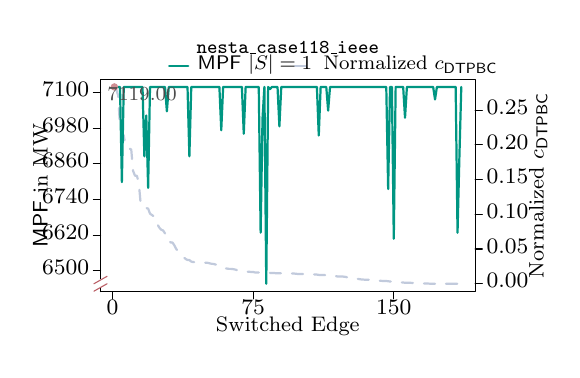
\begin{tikzpicture}[x=1pt,y=1pt]
\definecolor{fillColor}{RGB}{255,255,255}
\path[use as bounding box,fill=fillColor,fill opacity=0.00] (0,0) rectangle (440.85,271.01);
\begin{scope}
\path[clip] (  0.00,  0.00) rectangle (440.85,271.01);
\definecolor{drawColor}{RGB}{193,202,220}

\path[draw=drawColor,line width= 0.8pt,dash pattern=on 4pt off 4pt ,line join=round,line cap=round] ( 72.86,221.20) --
	( 74.44,219.00) --
	( 76.01,214.18) --
	( 77.59,188.49) --
	( 79.16,182.07) --
	( 80.74,180.34) --
	( 82.32,171.21) --
	( 83.89,170.15) --
	( 85.47,169.61) --
	( 87.04,168.51) --
	( 88.62,150.55) --
	( 90.19,146.66) --
	( 91.77,146.49) --
	( 93.35,140.91) --
	( 94.92,123.46) --
	( 96.50,123.46) --
	( 98.07,120.17) --
	( 99.65,119.41) --
	(101.23,118.98) --
	(102.80,114.72) --
	(104.38,113.62) --
	(105.95,112.48) --
	(107.53,111.67) --
	(109.10,105.59) --
	(110.68,102.89) --
	(112.26,101.15) --
	(113.83,100.60) --
	(115.41, 98.11) --
	(116.98, 92.32) --
	(118.56, 92.15) --
	(120.14, 90.55) --
	(121.71, 90.38) --
	(123.29, 88.01) --
	(124.86, 85.01) --
	(126.44, 82.77) --
	(128.01, 81.72) --
	(129.59, 79.14) --
	(131.17, 78.04) --
	(132.74, 76.60) --
	(134.32, 75.84) --
	(135.89, 75.76) --
	(137.47, 74.41) --
	(139.05, 74.07) --
	(140.62, 74.07) --
	(142.20, 74.07) --
	(143.77, 73.65) --
	(145.35, 73.56) --
	(146.92, 73.56) --
	(148.50, 73.48) --
	(150.08, 73.48) --
	(151.65, 73.31) --
	(153.23, 72.89) --
	(154.80, 72.55) --
	(156.38, 72.46) --
	(157.95, 71.91) --
	(159.53, 71.87) --
	(161.11, 71.36) --
	(162.68, 71.20) --
	(164.26, 69.76) --
	(165.83, 68.83) --
	(167.41, 68.58) --
	(168.99, 68.32) --
	(170.56, 68.32) --
	(172.14, 68.15) --
	(173.71, 67.90) --
	(175.29, 67.48) --
	(176.86, 67.05) --
	(178.44, 66.72) --
	(180.02, 66.38) --
	(181.59, 66.13) --
	(183.17, 65.96) --
	(184.74, 65.87) --
	(186.32, 65.87) --
	(187.90, 65.70) --
	(189.47, 65.70) --
	(191.05, 65.28) --
	(192.62, 65.20) --
	(194.20, 65.20) --
	(195.77, 65.11) --
	(197.35, 65.11) --
	(198.93, 65.03) --
	(200.50, 64.94) --
	(202.08, 64.94) --
	(203.65, 64.94) --
	(205.23, 64.86) --
	(206.80, 64.86) --
	(208.38, 64.69) --
	(209.96, 64.69) --
	(211.53, 64.69) --
	(213.11, 64.60) --
	(214.68, 64.60) --
	(216.26, 64.52) --
	(217.84, 64.52) --
	(219.41, 64.44) --
	(220.99, 64.44) --
	(222.56, 64.44) --
	(224.14, 64.35) --
	(225.71, 64.18) --
	(227.29, 64.01) --
	(228.87, 64.01) --
	(230.44, 64.01) --
	(232.02, 64.01) --
	(233.59, 63.93) --
	(235.17, 63.93) --
	(236.75, 63.76) --
	(238.32, 63.76) --
	(239.90, 63.67) --
	(241.47, 63.67) --
	(243.05, 63.51) --
	(244.62, 63.25) --
	(246.20, 63.25) --
	(247.78, 63.17) --
	(249.35, 63.08) --
	(250.93, 63.08) --
	(252.50, 63.00) --
	(254.08, 63.00) --
	(255.66, 62.41) --
	(257.23, 62.32) --
	(258.81, 62.28) --
	(260.38, 61.90) --
	(261.96, 61.90) --
	(263.53, 61.82) --
	(265.11, 61.82) --
	(266.69, 61.65) --
	(268.26, 61.31) --
	(269.84, 61.31) --
	(271.41, 61.22) --
	(272.99, 61.05) --
	(274.56, 60.29) --
	(276.14, 60.04) --
	(277.72, 59.87) --
	(279.29, 59.62) --
	(280.87, 59.36) --
	(282.44, 59.28) --
	(284.02, 59.20) --
	(285.60, 59.20) --
	(287.17, 59.11) --
	(288.75, 58.77) --
	(290.32, 58.69) --
	(291.90, 58.60) --
	(293.47, 58.52) --
	(295.05, 58.44) --
	(296.63, 58.27) --
	(298.20, 58.18) --
	(299.78, 58.18) --
	(301.35, 58.10) --
	(302.93, 57.93) --
	(304.51, 57.67) --
	(306.08, 57.67) --
	(307.66, 57.51) --
	(309.23, 57.34) --
	(310.81, 57.08) --
	(312.38, 57.08) --
	(313.96, 56.91) --
	(315.54, 56.83) --
	(317.11, 56.66) --
	(318.69, 56.58) --
	(320.26, 56.58) --
	(321.84, 56.58) --
	(323.41, 56.49) --
	(324.99, 56.49) --
	(326.57, 56.41) --
	(328.14, 56.32) --
	(329.72, 56.24) --
	(331.29, 56.07) --
	(332.87, 56.07) --
	(334.45, 55.98) --
	(336.02, 55.98) --
	(337.60, 55.90) --
	(339.17, 55.90) --
	(340.75, 55.90) --
	(342.32, 55.90) --
	(343.90, 55.82) --
	(345.48, 55.82) --
	(347.05, 55.82) --
	(348.63, 55.82) --
	(350.20, 55.82) --
	(351.78, 55.82) --
	(353.36, 55.82) --
	(354.93, 55.82) --
	(356.51, 55.82) --
	(358.08, 55.82) --
	(359.66, 55.82) --
	(361.23, 55.82) --
	(362.81, 55.82) --
	(364.39, 55.82);
\end{scope}
\begin{scope}
\path[clip] (  0.00,  0.00) rectangle (440.85,271.01);
\definecolor{drawColor}{RGB}{0,0,0}

\path[draw=drawColor,line width= 0.4pt,line join=round,line cap=round] ( 61.20, 49.20) --
	(376.05, 49.20) --
	(376.05,227.81) --
	( 61.20,227.81) --
	( 61.20, 49.20);
\end{scope}
\begin{scope}
\path[clip] (  0.00,  0.00) rectangle (440.85,271.01);
\definecolor{drawColor}{RGB}{0,0,0}

\path[draw=drawColor,line width= 0.4pt,line join=round,line cap=round] (376.05, 55.82) -- (376.05,201.65);

\path[draw=drawColor,line width= 0.4pt,line join=round,line cap=round] (376.05, 55.82) -- (382.05, 55.82);

\path[draw=drawColor,line width= 0.4pt,line join=round,line cap=round] (376.05, 84.98) -- (382.05, 84.98);

\path[draw=drawColor,line width= 0.4pt,line join=round,line cap=round] (376.05,114.15) -- (382.05,114.15);

\path[draw=drawColor,line width= 0.4pt,line join=round,line cap=round] (376.05,143.32) -- (382.05,143.32);

\path[draw=drawColor,line width= 0.4pt,line join=round,line cap=round] (376.05,172.49) -- (382.05,172.49);

\path[draw=drawColor,line width= 0.4pt,line join=round,line cap=round] (376.05,201.65) -- (382.05,201.65);

\node[text=drawColor,anchor=base west,inner sep=0pt, outer sep=0pt, scale=  1.00] at (385.65, 52.37) {0.00};

\node[text=drawColor,anchor=base west,inner sep=0pt, outer sep=0pt, scale=  1.00] at (385.65, 81.54) {0.05};

\node[text=drawColor,anchor=base west,inner sep=0pt, outer sep=0pt, scale=  1.00] at (385.65,110.71) {0.10};

\node[text=drawColor,anchor=base west,inner sep=0pt, outer sep=0pt, scale=  1.00] at (385.65,139.88) {0.15};

\node[text=drawColor,anchor=base west,inner sep=0pt, outer sep=0pt, scale=  1.00] at (385.65,169.04) {0.20};

\node[text=drawColor,anchor=base west,inner sep=0pt, outer sep=0pt, scale=  1.00] at (385.65,198.21) {0.25};
\end{scope}
\begin{scope}
\path[clip] (  0.00,  0.00) rectangle (440.85,271.01);
\definecolor{drawColor}{RGB}{0,150,130}

\path[draw=drawColor,line width= 0.8pt,line join=round,line cap=round] (118.89,238.60) -- (134.91,238.60);
\definecolor{drawColor}{RGB}{193,202,220}

\path[draw=drawColor,line width= 0.8pt,dash pattern=on 4pt off 4pt ,line join=round,line cap=round] (224.63,238.60) -- (240.65,238.60);
\definecolor{drawColor}{RGB}{0,0,0}

\node[text=drawColor,anchor=base,inner sep=0pt, outer sep=0pt, scale=  0.89] at (218.62,249.28) {\texttt{nesta\_case118\_ieee}};

\node[text=drawColor,anchor=base west,inner sep=0pt, outer sep=0pt, scale=  0.89] at (142.92,235.54) {$\mathsf{MPF}~|S|=1$};

\node[text=drawColor,anchor=base west,inner sep=0pt, outer sep=0pt, scale=  0.89] at (248.66,235.54) {Normalized~$c_\mathsf{DTPBC}$};
\end{scope}
\begin{scope}
\path[clip] (  0.00,  0.00) rectangle (440.85,271.01);
\definecolor{drawColor}{RGB}{0,0,0}

\path[draw=drawColor,line width= 0.4pt,line join=round,line cap=round] ( 61.20, 66.79) -- ( 61.20,216.46);

\path[draw=drawColor,line width= 0.4pt,line join=round,line cap=round] ( 61.20, 66.79) -- ( 55.20, 66.79);

\path[draw=drawColor,line width= 0.4pt,line join=round,line cap=round] ( 61.20, 96.72) -- ( 55.20, 96.72);

\path[draw=drawColor,line width= 0.4pt,line join=round,line cap=round] ( 61.20,126.66) -- ( 55.20,126.66);

\path[draw=drawColor,line width= 0.4pt,line join=round,line cap=round] ( 61.20,156.59) -- ( 55.20,156.59);

\path[draw=drawColor,line width= 0.4pt,line join=round,line cap=round] ( 61.20,186.52) -- ( 55.20,186.52);

\path[draw=drawColor,line width= 0.4pt,line join=round,line cap=round] ( 61.20,216.46) -- ( 55.20,216.46);

\node[text=drawColor,anchor=base east,inner sep=0pt, outer sep=0pt, scale=  1.00] at ( 51.60, 63.35) {6500};

\node[text=drawColor,anchor=base east,inner sep=0pt, outer sep=0pt, scale=  1.00] at ( 51.60, 93.28) {6620};

\node[text=drawColor,anchor=base east,inner sep=0pt, outer sep=0pt, scale=  1.00] at ( 51.60,123.21) {6740};

\node[text=drawColor,anchor=base east,inner sep=0pt, outer sep=0pt, scale=  1.00] at ( 51.60,153.15) {6860};

\node[text=drawColor,anchor=base east,inner sep=0pt, outer sep=0pt, scale=  1.00] at ( 51.60,183.08) {6980};

\node[text=drawColor,anchor=base east,inner sep=0pt, outer sep=0pt, scale=  1.00] at ( 51.60,213.01) {7100};
\end{scope}
\begin{scope}
\path[clip] (  0.00,  0.00) rectangle (440.85,271.01);
\definecolor{drawColor}{RGB}{255,255,255}
\definecolor{fillColor}{RGB}{255,255,255}

\path[draw=drawColor,line width= 0.4pt,line join=round,line cap=round,fill=fillColor] ( 55.69, 52.69) rectangle ( 66.71, 58.94);
\definecolor{drawColor}{RGB}{188,97,104}

\path[draw=drawColor,line width= 0.4pt,line join=round,line cap=round] ( 55.69, 49.56) -- ( 66.71, 55.82);

\path[draw=drawColor,line width= 0.4pt,line join=round,line cap=round] ( 55.69, 55.82) -- ( 66.71, 62.07);
\end{scope}
\begin{scope}
\path[clip] ( 61.20, 49.20) rectangle (376.05,227.81);
\definecolor{drawColor}{RGB}{0,150,130}

\path[draw=drawColor,line width= 0.8pt,line join=round,line cap=round] ( 72.86,221.20) --
	( 74.44,221.20) --
	( 76.01,221.20) --
	( 77.59,221.20) --
	( 79.16,141.26) --
	( 80.74,221.20) --
	( 82.32,221.20) --
	( 83.89,221.20) --
	( 85.47,221.20) --
	( 87.04,221.20) --
	( 88.62,221.20) --
	( 90.19,221.20) --
	( 91.77,221.20) --
	( 93.35,221.20) --
	( 94.92,221.20) --
	( 96.50,221.20) --
	( 98.07,162.79) --
	( 99.65,197.25) --
	(101.23,136.39) --
	(102.80,221.20) --
	(104.38,221.20) --
	(105.95,221.20) --
	(107.53,221.20) --
	(109.10,221.20) --
	(110.68,221.20) --
	(112.26,221.20) --
	(113.83,221.20) --
	(115.41,221.20) --
	(116.98,200.75) --
	(118.56,221.20) --
	(120.14,221.20) --
	(121.71,221.20) --
	(123.29,221.20) --
	(124.86,221.20) --
	(126.44,221.20) --
	(128.01,221.20) --
	(129.59,221.20) --
	(131.17,221.20) --
	(132.74,221.20) --
	(134.32,221.20) --
	(135.89,162.84) --
	(137.47,221.20) --
	(139.05,221.20) --
	(140.62,221.20) --
	(142.20,221.20) --
	(143.77,221.20) --
	(145.35,221.20) --
	(146.92,221.20) --
	(148.50,221.20) --
	(150.08,221.20) --
	(151.65,221.20) --
	(153.23,221.20) --
	(154.80,221.20) --
	(156.38,221.20) --
	(157.95,221.20) --
	(159.53,221.20) --
	(161.11,221.20) --
	(162.68,184.78) --
	(164.26,221.20) --
	(165.83,221.20) --
	(167.41,221.20) --
	(168.99,221.20) --
	(170.56,221.20) --
	(172.14,221.20) --
	(173.71,221.20) --
	(175.29,221.20) --
	(176.86,221.20) --
	(178.44,221.20) --
	(180.02,221.20) --
	(181.59,181.82) --
	(183.17,221.20) --
	(184.74,221.20) --
	(186.32,221.20) --
	(187.90,221.20) --
	(189.47,221.20) --
	(191.05,221.20) --
	(192.62,221.20) --
	(194.20,221.20) --
	(195.77, 98.72) --
	(197.35,194.73) --
	(198.93,221.20) --
	(200.50, 55.82) --
	(202.08,221.20) --
	(203.65,219.45) --
	(205.23,221.20) --
	(206.80,221.20) --
	(208.38,221.20) --
	(209.96,221.20) --
	(211.53,188.02) --
	(213.11,221.20) --
	(214.68,221.20) --
	(216.26,221.20) --
	(217.84,221.20) --
	(219.41,221.20) --
	(220.99,221.20) --
	(222.56,221.20) --
	(224.14,221.20) --
	(225.71,221.20) --
	(227.29,221.20) --
	(228.87,221.20) --
	(230.44,221.20) --
	(232.02,221.20) --
	(233.59,221.20) --
	(235.17,221.20) --
	(236.75,221.20) --
	(238.32,221.20) --
	(239.90,221.20) --
	(241.47,221.20) --
	(243.05,221.20) --
	(244.62,180.36) --
	(246.20,221.20) --
	(247.78,221.20) --
	(249.35,221.20) --
	(250.93,221.20) --
	(252.50,201.27) --
	(254.08,221.20) --
	(255.66,221.20) --
	(257.23,221.20) --
	(258.81,221.20) --
	(260.38,221.20) --
	(261.96,221.20) --
	(263.53,221.20) --
	(265.11,221.20) --
	(266.69,221.20) --
	(268.26,221.20) --
	(269.84,221.20) --
	(271.41,221.20) --
	(272.99,221.20) --
	(274.56,221.20) --
	(276.14,221.20) --
	(277.72,221.20) --
	(279.29,221.20) --
	(280.87,221.20) --
	(282.44,221.20) --
	(284.02,221.20) --
	(285.60,221.20) --
	(287.17,221.20) --
	(288.75,221.20) --
	(290.32,221.20) --
	(291.90,221.20) --
	(293.47,221.20) --
	(295.05,221.20) --
	(296.63,221.20) --
	(298.20,221.20) --
	(299.78,221.20) --
	(301.35,221.20) --
	(302.93,135.43) --
	(304.51,221.20) --
	(306.08,221.20) --
	(307.66, 93.62) --
	(309.23,221.20) --
	(310.81,221.20) --
	(312.38,221.20) --
	(313.96,221.20) --
	(315.54,221.20) --
	(317.11,195.34) --
	(318.69,221.20) --
	(320.26,221.20) --
	(321.84,221.20) --
	(323.41,221.20) --
	(324.99,221.20) --
	(326.57,221.20) --
	(328.14,221.20) --
	(329.72,221.20) --
	(331.29,221.20) --
	(332.87,221.20) --
	(334.45,221.20) --
	(336.02,221.20) --
	(337.60,221.20) --
	(339.17,221.20) --
	(340.75,221.20) --
	(342.32,210.67) --
	(343.90,221.20) --
	(345.48,221.20) --
	(347.05,221.20) --
	(348.63,221.20) --
	(350.20,221.20) --
	(351.78,221.20) --
	(353.36,221.20) --
	(354.93,221.20) --
	(356.51,221.20) --
	(358.08,221.20) --
	(359.66,221.20) --
	(361.23, 98.72) --
	(362.81,162.84) --
	(364.39,221.20);
\end{scope}
\begin{scope}
\path[clip] ( 61.20, 49.20) rectangle (376.05,227.81);
\definecolor{fillColor}{RGB}{207,142,147}

\path[fill=fillColor] ( 72.86,221.20) circle (  3.15);
\end{scope}
\begin{scope}
\path[clip] ( 61.20, 49.20) rectangle (376.05,227.81);
\definecolor{drawColor}{gray}{0.30}

\node[text=drawColor,anchor=base,inner sep=0pt, outer sep=0pt, scale=  0.90] at ( 96.18,210.04) {7119.00};
\end{scope}
\begin{scope}
\path[clip] (  0.00,  0.00) rectangle (440.85,271.01);
\definecolor{drawColor}{RGB}{0,0,0}

\path[draw=drawColor,line width= 0.4pt,line join=round,line cap=round] ( 71.29, 49.20) -- (307.66, 49.20);

\path[draw=drawColor,line width= 0.4pt,line join=round,line cap=round] ( 71.29, 49.20) -- ( 71.29, 43.20);

\path[draw=drawColor,line width= 0.4pt,line join=round,line cap=round] (189.47, 49.20) -- (189.47, 43.20);

\path[draw=drawColor,line width= 0.4pt,line join=round,line cap=round] (307.66, 49.20) -- (307.66, 43.20);

\node[text=drawColor,anchor=base,inner sep=0pt, outer sep=0pt, scale=  1.00] at ( 71.29, 30.00) {0};

\node[text=drawColor,anchor=base,inner sep=0pt, outer sep=0pt, scale=  1.00] at (189.47, 30.00) {75};

\node[text=drawColor,anchor=base,inner sep=0pt, outer sep=0pt, scale=  1.00] at (307.66, 30.00) {150};

\node[text=drawColor,anchor=base,inner sep=0pt, outer sep=0pt, scale=  0.95] at (218.62, 15.60) {Switched Edge};

\node[text=drawColor,rotate= 90.00,anchor=base,inner sep=0pt, outer sep=0pt, scale=  0.95] at ( 16.80,138.51) {$\mathsf{MPF}$ in~$\mathrm{MW}$};

\node[text=drawColor,rotate= 90.00,anchor=base,inner sep=0pt, outer sep=0pt, scale=  0.95] at (433.65,138.51) {Normalized~$c_\mathsf{DTPBC}$};
\end{scope}
\end{tikzpicture}
%
    \label{plot:SwitchingBetweenness_nesta_case118_ieee_dtpbc_mpf_cutY}
  \end{subfigure}
  % 
  \caption{Results of the simulations for the~\gls{dtp} betweenness centrality
  on cases \texttt{nesta\_case30\_as} to~\texttt{nesta\_case118\_ieee}.}%
  % 
  \label{fig:Switching_Betweenness_Centrality_Plot_Cut_Y_29_to_89}%
\end{figure}%
% 

%%%%%%%%%%%%%%%%%%%%%%%%%%%%%%%%%%%%%%%%%%%%%%%%%%%%%%%%%%%%%%%%%%%%%%%%%%%%%%%%
\newpage
%
\begin{figure}[H]%
  %
  \begin{subfigure}[t]{.5\textwidth}%
    \centering%
    % Created by tikzDevice version 0.10.1 on 2018-01-31 10:27:24
% !TEX encoding = UTF-8 Unicode
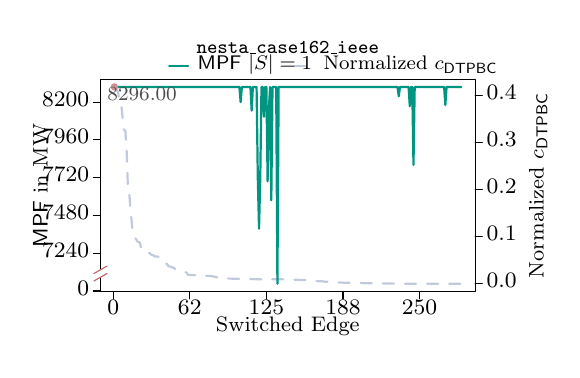
\begin{tikzpicture}[x=1pt,y=1pt]
\definecolor{fillColor}{RGB}{255,255,255}
\path[use as bounding box,fill=fillColor,fill opacity=0.00] (0,0) rectangle (440.85,271.01);
\begin{scope}
\path[clip] (  0.00,  0.00) rectangle (440.85,271.01);
\definecolor{drawColor}{RGB}{193,202,220}

\path[draw=drawColor,line width= 0.8pt,dash pattern=on 4pt off 4pt ,line join=round,line cap=round] ( 72.86,221.20) --
	( 73.89,220.50) --
	( 74.92,218.50) --
	( 75.95,217.11) --
	( 76.98,209.42) --
	( 78.01,207.65) --
	( 79.04,202.94) --
	( 80.07,192.07) --
	( 81.10,185.14) --
	( 82.13,184.05) --
	( 83.16,167.77) --
	( 84.19,138.35) --
	( 85.22,135.15) --
	( 86.25,119.11) --
	( 87.28,109.62) --
	( 88.31, 98.87) --
	( 89.34, 96.90) --
	( 90.37, 94.25) --
	( 91.40, 92.77) --
	( 92.43, 91.17) --
	( 93.46, 90.77) --
	( 94.49, 89.83) --
	( 95.52, 84.31) --
	( 96.55, 83.34) --
	( 97.58, 83.04) --
	( 98.61, 82.99) --
	( 99.64, 82.19) --
	(100.67, 81.95) --
	(101.70, 81.57) --
	(102.73, 81.46) --
	(103.76, 80.14) --
	(104.79, 79.98) --
	(105.82, 79.66) --
	(106.86, 78.72) --
	(107.89, 78.69) --
	(108.92, 78.69) --
	(109.95, 78.52) --
	(110.98, 77.59) --
	(112.01, 76.92) --
	(113.04, 75.25) --
	(114.07, 72.91) --
	(115.10, 72.82) --
	(116.13, 72.59) --
	(117.16, 72.38) --
	(118.19, 70.83) --
	(119.22, 70.26) --
	(120.25, 70.15) --
	(121.28, 69.53) --
	(122.31, 69.47) --
	(123.34, 68.65) --
	(124.37, 67.97) --
	(125.40, 67.00) --
	(126.43, 66.75) --
	(127.46, 66.56) --
	(128.49, 66.26) --
	(129.52, 66.02) --
	(130.55, 65.94) --
	(131.58, 65.66) --
	(132.61, 65.41) --
	(133.64, 65.29) --
	(134.67, 63.29) --
	(135.70, 63.26) --
	(136.73, 63.25) --
	(137.76, 63.20) --
	(138.79, 63.17) --
	(139.82, 63.08) --
	(140.85, 62.98) --
	(141.88, 62.89) --
	(142.91, 62.84) --
	(143.94, 62.84) --
	(144.97, 62.81) --
	(146.00, 62.79) --
	(147.03, 62.73) --
	(148.06, 62.73) --
	(149.09, 62.60) --
	(150.12, 62.58) --
	(151.15, 62.43) --
	(152.18, 62.42) --
	(153.21, 62.39) --
	(154.24, 62.22) --
	(155.27, 62.11) --
	(156.30, 61.92) --
	(157.33, 61.55) --
	(158.36, 61.39) --
	(159.39, 61.08) --
	(160.42, 60.86) --
	(161.45, 60.80) --
	(162.48, 60.46) --
	(163.51, 60.45) --
	(164.54, 60.40) --
	(165.57, 60.37) --
	(166.60, 60.37) --
	(167.63, 60.18) --
	(168.66, 60.15) --
	(169.69, 60.11) --
	(170.72, 60.11) --
	(171.75, 60.10) --
	(172.78, 60.07) --
	(173.81, 60.05) --
	(174.84, 59.95) --
	(175.87, 59.95) --
	(176.90, 59.92) --
	(177.93, 59.90) --
	(178.96, 59.90) --
	(179.99, 59.90) --
	(181.02, 59.87) --
	(182.05, 59.83) --
	(183.08, 59.81) --
	(184.11, 59.80) --
	(185.14, 59.78) --
	(186.17, 59.78) --
	(187.20, 59.75) --
	(188.23, 59.72) --
	(189.26, 59.71) --
	(190.30, 59.69) --
	(191.33, 59.68) --
	(192.36, 59.66) --
	(193.39, 59.65) --
	(194.42, 59.63) --
	(195.45, 59.63) --
	(196.48, 59.63) --
	(197.51, 59.63) --
	(198.54, 59.62) --
	(199.57, 59.60) --
	(200.60, 59.60) --
	(201.63, 59.58) --
	(202.66, 59.58) --
	(203.69, 59.58) --
	(204.72, 59.58) --
	(205.75, 59.58) --
	(206.78, 59.57) --
	(207.81, 59.57) --
	(208.84, 59.57) --
	(209.87, 59.54) --
	(210.90, 59.54) --
	(211.93, 59.52) --
	(212.96, 59.52) --
	(213.99, 59.49) --
	(215.02, 59.48) --
	(216.05, 59.42) --
	(217.08, 59.37) --
	(218.11, 59.36) --
	(219.14, 59.33) --
	(220.17, 59.28) --
	(221.20, 59.19) --
	(222.23, 59.18) --
	(223.26, 59.16) --
	(224.29, 59.13) --
	(225.32, 59.10) --
	(226.35, 59.09) --
	(227.38, 59.09) --
	(228.41, 59.06) --
	(229.44, 58.99) --
	(230.47, 58.99) --
	(231.50, 58.98) --
	(232.53, 58.90) --
	(233.56, 58.90) --
	(234.59, 58.87) --
	(235.62, 58.72) --
	(236.65, 58.69) --
	(237.68, 58.69) --
	(238.71, 58.57) --
	(239.74, 58.54) --
	(240.77, 58.40) --
	(241.80, 58.24) --
	(242.83, 58.06) --
	(243.86, 58.00) --
	(244.89, 57.98) --
	(245.92, 57.95) --
	(246.95, 57.89) --
	(247.98, 57.80) --
	(249.01, 57.68) --
	(250.04, 57.48) --
	(251.07, 57.42) --
	(252.10, 57.40) --
	(253.13, 57.34) --
	(254.16, 57.27) --
	(255.19, 57.19) --
	(256.22, 57.15) --
	(257.25, 57.06) --
	(258.28, 56.94) --
	(259.31, 56.88) --
	(260.34, 56.88) --
	(261.37, 56.84) --
	(262.40, 56.80) --
	(263.43, 56.78) --
	(264.46, 56.77) --
	(265.49, 56.72) --
	(266.52, 56.71) --
	(267.55, 56.65) --
	(268.58, 56.63) --
	(269.61, 56.62) --
	(270.64, 56.57) --
	(271.67, 56.56) --
	(272.70, 56.54) --
	(273.74, 56.53) --
	(274.77, 56.53) --
	(275.80, 56.53) --
	(276.83, 56.50) --
	(277.86, 56.41) --
	(278.89, 56.38) --
	(279.92, 56.38) --
	(280.95, 56.38) --
	(281.98, 56.33) --
	(283.01, 56.28) --
	(284.04, 56.27) --
	(285.07, 56.24) --
	(286.10, 56.24) --
	(287.13, 56.21) --
	(288.16, 56.19) --
	(289.19, 56.19) --
	(290.22, 56.13) --
	(291.25, 56.13) --
	(292.28, 56.12) --
	(293.31, 56.06) --
	(294.34, 56.06) --
	(295.37, 56.04) --
	(296.40, 56.04) --
	(297.43, 56.04) --
	(298.46, 56.03) --
	(299.49, 56.03) --
	(300.52, 56.01) --
	(301.55, 56.00) --
	(302.58, 56.00) --
	(303.61, 55.98) --
	(304.64, 55.98) --
	(305.67, 55.97) --
	(306.70, 55.97) --
	(307.73, 55.97) --
	(308.76, 55.94) --
	(309.79, 55.92) --
	(310.82, 55.92) --
	(311.85, 55.92) --
	(312.88, 55.91) --
	(313.91, 55.91) --
	(314.94, 55.89) --
	(315.97, 55.88) --
	(317.00, 55.88) --
	(318.03, 55.86) --
	(319.06, 55.86) --
	(320.09, 55.86) --
	(321.12, 55.86) --
	(322.15, 55.85) --
	(323.18, 55.85) --
	(324.21, 55.85) --
	(325.24, 55.85) --
	(326.27, 55.85) --
	(327.30, 55.85) --
	(328.33, 55.85) --
	(329.36, 55.85) --
	(330.39, 55.82) --
	(331.42, 55.82) --
	(332.45, 55.82) --
	(333.48, 55.82) --
	(334.51, 55.82) --
	(335.54, 55.82) --
	(336.57, 55.82) --
	(337.60, 55.82) --
	(338.63, 55.82) --
	(339.66, 55.82) --
	(340.69, 55.82) --
	(341.72, 55.82) --
	(342.75, 55.82) --
	(343.78, 55.82) --
	(344.81, 55.82) --
	(345.84, 55.82) --
	(346.87, 55.82) --
	(347.90, 55.82) --
	(348.93, 55.82) --
	(349.96, 55.82) --
	(350.99, 55.82) --
	(352.02, 55.82) --
	(353.05, 55.82) --
	(354.08, 55.82) --
	(355.11, 55.82) --
	(356.15, 55.82) --
	(357.18, 55.82) --
	(358.21, 55.82) --
	(359.24, 55.82) --
	(360.27, 55.82) --
	(361.30, 55.82) --
	(362.33, 55.82) --
	(363.36, 55.82) --
	(364.39, 55.82);
\end{scope}
\begin{scope}
\path[clip] (  0.00,  0.00) rectangle (440.85,271.01);
\definecolor{drawColor}{RGB}{0,0,0}

\path[draw=drawColor,line width= 0.4pt,line join=round,line cap=round] ( 61.20, 49.20) --
	(376.05, 49.20) --
	(376.05,227.81) --
	( 61.20,227.81) --
	( 61.20, 49.20);
\end{scope}
\begin{scope}
\path[clip] (  0.00,  0.00) rectangle (440.85,271.01);
\definecolor{drawColor}{RGB}{0,0,0}

\path[draw=drawColor,line width= 0.4pt,line join=round,line cap=round] (376.05, 55.82) -- (376.05,213.76);

\path[draw=drawColor,line width= 0.4pt,line join=round,line cap=round] (376.05, 55.82) -- (382.05, 55.82);

\path[draw=drawColor,line width= 0.4pt,line join=round,line cap=round] (376.05, 95.30) -- (382.05, 95.30);

\path[draw=drawColor,line width= 0.4pt,line join=round,line cap=round] (376.05,134.79) -- (382.05,134.79);

\path[draw=drawColor,line width= 0.4pt,line join=round,line cap=round] (376.05,174.27) -- (382.05,174.27);

\path[draw=drawColor,line width= 0.4pt,line join=round,line cap=round] (376.05,213.76) -- (382.05,213.76);

\node[text=drawColor,anchor=base west,inner sep=0pt, outer sep=0pt, scale=  1.00] at (385.65, 52.37) {0.0};

\node[text=drawColor,anchor=base west,inner sep=0pt, outer sep=0pt, scale=  1.00] at (385.65, 91.86) {0.1};

\node[text=drawColor,anchor=base west,inner sep=0pt, outer sep=0pt, scale=  1.00] at (385.65,131.34) {0.2};

\node[text=drawColor,anchor=base west,inner sep=0pt, outer sep=0pt, scale=  1.00] at (385.65,170.83) {0.3};

\node[text=drawColor,anchor=base west,inner sep=0pt, outer sep=0pt, scale=  1.00] at (385.65,210.32) {0.4};
\end{scope}
\begin{scope}
\path[clip] (  0.00,  0.00) rectangle (440.85,271.01);
\definecolor{drawColor}{RGB}{0,150,130}

\path[draw=drawColor,line width= 0.8pt,line join=round,line cap=round] (118.89,238.60) -- (134.91,238.60);
\definecolor{drawColor}{RGB}{193,202,220}

\path[draw=drawColor,line width= 0.8pt,dash pattern=on 4pt off 4pt ,line join=round,line cap=round] (224.63,238.60) -- (240.65,238.60);
\definecolor{drawColor}{RGB}{0,0,0}

\node[text=drawColor,anchor=base,inner sep=0pt, outer sep=0pt, scale=  0.89] at (218.62,249.28) {\texttt{nesta\_case162\_ieee}};

\node[text=drawColor,anchor=base west,inner sep=0pt, outer sep=0pt, scale=  0.89] at (142.92,235.54) {$\mathsf{MPF}~|S|=1$};

\node[text=drawColor,anchor=base west,inner sep=0pt, outer sep=0pt, scale=  0.89] at (248.66,235.54) {Normalized~$c_\mathsf{DTPBC}$};
\end{scope}
\begin{scope}
\path[clip] (  0.00,  0.00) rectangle (440.85,271.01);
\definecolor{drawColor}{RGB}{0,0,0}

\path[draw=drawColor,line width= 0.4pt,line join=round,line cap=round] ( 61.20, 49.73) -- ( 61.20,208.50);

\path[draw=drawColor,line width= 0.4pt,line join=round,line cap=round] ( 61.20, 49.73) -- ( 55.20, 49.73);

\path[draw=drawColor,line width= 0.4pt,line join=round,line cap=round] ( 61.20, 81.48) -- ( 55.20, 81.48);

\path[draw=drawColor,line width= 0.4pt,line join=round,line cap=round] ( 61.20,113.24) -- ( 55.20,113.24);

\path[draw=drawColor,line width= 0.4pt,line join=round,line cap=round] ( 61.20,144.99) -- ( 55.20,144.99);

\path[draw=drawColor,line width= 0.4pt,line join=round,line cap=round] ( 61.20,176.74) -- ( 55.20,176.74);

\path[draw=drawColor,line width= 0.4pt,line join=round,line cap=round] ( 61.20,208.50) -- ( 55.20,208.50);

\node[text=drawColor,anchor=base east,inner sep=0pt, outer sep=0pt, scale=  1.00] at ( 51.60, 46.29) {0};

\node[text=drawColor,anchor=base east,inner sep=0pt, outer sep=0pt, scale=  1.00] at ( 51.60, 78.04) {7240};

\node[text=drawColor,anchor=base east,inner sep=0pt, outer sep=0pt, scale=  1.00] at ( 51.60,109.79) {7480};

\node[text=drawColor,anchor=base east,inner sep=0pt, outer sep=0pt, scale=  1.00] at ( 51.60,141.55) {7720};

\node[text=drawColor,anchor=base east,inner sep=0pt, outer sep=0pt, scale=  1.00] at ( 51.60,173.30) {7960};

\node[text=drawColor,anchor=base east,inner sep=0pt, outer sep=0pt, scale=  1.00] at ( 51.60,205.05) {8200};
\end{scope}
\begin{scope}
\path[clip] (  0.00,  0.00) rectangle (440.85,271.01);
\definecolor{drawColor}{RGB}{255,255,255}
\definecolor{fillColor}{RGB}{255,255,255}

\path[draw=drawColor,line width= 0.4pt,line join=round,line cap=round,fill=fillColor] ( 55.69, 61.30) rectangle ( 66.71, 67.56);
\definecolor{drawColor}{RGB}{188,97,104}

\path[draw=drawColor,line width= 0.4pt,line join=round,line cap=round] ( 55.69, 58.18) -- ( 66.71, 64.43);

\path[draw=drawColor,line width= 0.4pt,line join=round,line cap=round] ( 55.69, 64.43) -- ( 66.71, 70.68);
\end{scope}
\begin{scope}
\path[clip] ( 61.20, 49.20) rectangle (376.05,227.81);
\definecolor{drawColor}{RGB}{0,150,130}

\path[draw=drawColor,line width= 0.8pt,line join=round,line cap=round] ( 72.86,221.20) --
	( 73.89,221.20) --
	( 74.92,221.20) --
	( 75.95,221.20) --
	( 76.98,221.20) --
	( 78.01,221.20) --
	( 79.04,221.20) --
	( 80.07,221.20) --
	( 81.10,221.20) --
	( 82.13,221.20) --
	( 83.16,221.20) --
	( 84.19,221.20) --
	( 85.22,221.20) --
	( 86.25,221.20) --
	( 87.28,221.20) --
	( 88.31,221.20) --
	( 89.34,221.20) --
	( 90.37,221.20) --
	( 91.40,221.20) --
	( 92.43,221.20) --
	( 93.46,221.20) --
	( 94.49,221.20) --
	( 95.52,221.20) --
	( 96.55,221.20) --
	( 97.58,221.20) --
	( 98.61,221.20) --
	( 99.64,221.20) --
	(100.67,221.20) --
	(101.70,221.20) --
	(102.73,221.20) --
	(103.76,221.20) --
	(104.79,221.20) --
	(105.82,221.20) --
	(106.86,221.20) --
	(107.89,221.20) --
	(108.92,221.20) --
	(109.95,221.20) --
	(110.98,221.20) --
	(112.01,221.20) --
	(113.04,221.20) --
	(114.07,221.20) --
	(115.10,221.20) --
	(116.13,221.20) --
	(117.16,221.20) --
	(118.19,221.20) --
	(119.22,221.20) --
	(120.25,221.20) --
	(121.28,221.20) --
	(122.31,221.20) --
	(123.34,221.20) --
	(124.37,221.20) --
	(125.40,221.20) --
	(126.43,221.20) --
	(127.46,221.20) --
	(128.49,221.20) --
	(129.52,221.20) --
	(130.55,221.20) --
	(131.58,221.20) --
	(132.61,221.20) --
	(133.64,221.20) --
	(134.67,221.20) --
	(135.70,221.20) --
	(136.73,221.20) --
	(137.76,221.20) --
	(138.79,221.20) --
	(139.82,221.20) --
	(140.85,221.20) --
	(141.88,221.20) --
	(142.91,221.20) --
	(143.94,221.20) --
	(144.97,221.20) --
	(146.00,221.20) --
	(147.03,221.20) --
	(148.06,221.20) --
	(149.09,221.20) --
	(150.12,221.20) --
	(151.15,221.20) --
	(152.18,221.20) --
	(153.21,221.20) --
	(154.24,221.20) --
	(155.27,221.20) --
	(156.30,221.20) --
	(157.33,221.20) --
	(158.36,221.20) --
	(159.39,221.20) --
	(160.42,221.20) --
	(161.45,221.20) --
	(162.48,221.20) --
	(163.51,221.20) --
	(164.54,221.20) --
	(165.57,221.20) --
	(166.60,221.20) --
	(167.63,221.20) --
	(168.66,221.20) --
	(169.69,221.20) --
	(170.72,221.20) --
	(171.75,221.20) --
	(172.78,221.20) --
	(173.81,221.20) --
	(174.84,221.20) --
	(175.87,221.20) --
	(176.90,221.20) --
	(177.93,221.20) --
	(178.96,208.50) --
	(179.99,221.20) --
	(181.02,221.20) --
	(182.05,221.20) --
	(183.08,221.20) --
	(184.11,221.20) --
	(185.14,221.20) --
	(186.17,221.20) --
	(187.20,221.20) --
	(188.23,201.35) --
	(189.26,221.20) --
	(190.30,221.20) --
	(191.33,221.20) --
	(192.36,221.20) --
	(193.39,144.72) --
	(194.42,102.12) --
	(195.45,144.46) --
	(196.48,221.20) --
	(197.51,221.20) --
	(198.54,196.19) --
	(199.57,221.20) --
	(200.60,221.20) --
	(201.63,141.81) --
	(202.66,201.62) --
	(203.69,221.20) --
	(204.72,125.94) --
	(205.75,221.20) --
	(206.78,221.20) --
	(207.81,221.20) --
	(208.84,221.20) --
	(209.87, 55.82) --
	(210.90,221.20) --
	(211.93,221.20) --
	(212.96,221.20) --
	(213.99,221.20) --
	(215.02,221.20) --
	(216.05,221.20) --
	(217.08,221.20) --
	(218.11,221.20) --
	(219.14,221.20) --
	(220.17,221.20) --
	(221.20,221.20) --
	(222.23,221.20) --
	(223.26,221.20) --
	(224.29,221.20) --
	(225.32,221.20) --
	(226.35,221.20) --
	(227.38,221.20) --
	(228.41,221.20) --
	(229.44,221.20) --
	(230.47,221.20) --
	(231.50,221.20) --
	(232.53,221.20) --
	(233.56,221.20) --
	(234.59,221.20) --
	(235.62,221.20) --
	(236.65,221.20) --
	(237.68,221.20) --
	(238.71,221.20) --
	(239.74,221.20) --
	(240.77,221.20) --
	(241.80,221.20) --
	(242.83,221.20) --
	(243.86,221.20) --
	(244.89,221.20) --
	(245.92,221.20) --
	(246.95,221.20) --
	(247.98,221.20) --
	(249.01,221.20) --
	(250.04,221.20) --
	(251.07,221.20) --
	(252.10,221.20) --
	(253.13,221.20) --
	(254.16,221.20) --
	(255.19,221.20) --
	(256.22,221.20) --
	(257.25,221.20) --
	(258.28,221.20) --
	(259.31,221.20) --
	(260.34,221.20) --
	(261.37,221.20) --
	(262.40,221.20) --
	(263.43,221.20) --
	(264.46,221.20) --
	(265.49,221.20) --
	(266.52,221.20) --
	(267.55,221.20) --
	(268.58,221.20) --
	(269.61,221.20) --
	(270.64,221.20) --
	(271.67,221.20) --
	(272.70,221.20) --
	(273.74,221.20) --
	(274.77,221.20) --
	(275.80,221.20) --
	(276.83,221.20) --
	(277.86,221.20) --
	(278.89,221.20) --
	(279.92,221.20) --
	(280.95,221.20) --
	(281.98,221.20) --
	(283.01,221.20) --
	(284.04,221.20) --
	(285.07,221.20) --
	(286.10,221.20) --
	(287.13,221.20) --
	(288.16,221.20) --
	(289.19,221.20) --
	(290.22,221.20) --
	(291.25,221.20) --
	(292.28,221.20) --
	(293.31,221.20) --
	(294.34,221.20) --
	(295.37,221.20) --
	(296.40,221.20) --
	(297.43,221.20) --
	(298.46,221.20) --
	(299.49,221.20) --
	(300.52,221.20) --
	(301.55,221.20) --
	(302.58,221.20) --
	(303.61,221.20) --
	(304.64,221.20) --
	(305.67,221.20) --
	(306.70,221.20) --
	(307.73,221.20) --
	(308.76,221.20) --
	(309.79,221.20) --
	(310.82,221.20) --
	(311.85,213.36) --
	(312.88,221.20) --
	(313.91,221.20) --
	(314.94,221.20) --
	(315.97,221.20) --
	(317.00,221.20) --
	(318.03,221.20) --
	(319.06,221.20) --
	(320.09,221.20) --
	(321.12,204.96) --
	(322.15,221.20) --
	(323.18,221.20) --
	(324.21,155.71) --
	(325.24,221.20) --
	(326.27,221.20) --
	(327.30,221.20) --
	(328.33,221.20) --
	(329.36,221.20) --
	(330.39,221.20) --
	(331.42,221.20) --
	(332.45,221.20) --
	(333.48,221.20) --
	(334.51,221.20) --
	(335.54,221.20) --
	(336.57,221.20) --
	(337.60,221.20) --
	(338.63,221.20) --
	(339.66,221.20) --
	(340.69,221.20) --
	(341.72,221.20) --
	(342.75,221.20) --
	(343.78,221.20) --
	(344.81,221.20) --
	(345.84,221.20) --
	(346.87,221.20) --
	(347.90,221.20) --
	(348.93,221.20) --
	(349.96,221.20) --
	(350.99,206.03) --
	(352.02,221.20) --
	(353.05,221.20) --
	(354.08,221.20) --
	(355.11,221.20) --
	(356.15,221.20) --
	(357.18,221.20) --
	(358.21,221.20) --
	(359.24,221.20) --
	(360.27,221.20) --
	(361.30,221.20) --
	(362.33,221.20) --
	(363.36,221.20) --
	(364.39,221.20);
\end{scope}
\begin{scope}
\path[clip] ( 61.20, 49.20) rectangle (376.05,227.81);
\definecolor{fillColor}{RGB}{207,142,147}

\path[fill=fillColor] ( 72.86,221.20) circle (  3.15);
\end{scope}
\begin{scope}
\path[clip] ( 61.20, 49.20) rectangle (376.05,227.81);
\definecolor{drawColor}{gray}{0.30}

\node[text=drawColor,anchor=base,inner sep=0pt, outer sep=0pt, scale=  0.90] at ( 96.18,210.04) {8296.00};
\end{scope}
\begin{scope}
\path[clip] (  0.00,  0.00) rectangle (440.85,271.01);
\definecolor{drawColor}{RGB}{0,0,0}

\path[draw=drawColor,line width= 0.4pt,line join=round,line cap=round] ( 71.83, 49.20) -- (329.36, 49.20);

\path[draw=drawColor,line width= 0.4pt,line join=round,line cap=round] ( 71.83, 49.20) -- ( 71.83, 43.20);

\path[draw=drawColor,line width= 0.4pt,line join=round,line cap=round] (136.21, 49.20) -- (136.21, 43.20);

\path[draw=drawColor,line width= 0.4pt,line join=round,line cap=round] (200.60, 49.20) -- (200.60, 43.20);

\path[draw=drawColor,line width= 0.4pt,line join=round,line cap=round] (264.98, 49.20) -- (264.98, 43.20);

\path[draw=drawColor,line width= 0.4pt,line join=round,line cap=round] (329.36, 49.20) -- (329.36, 43.20);

\node[text=drawColor,anchor=base,inner sep=0pt, outer sep=0pt, scale=  1.00] at ( 71.83, 30.00) {0};

\node[text=drawColor,anchor=base,inner sep=0pt, outer sep=0pt, scale=  1.00] at (136.21, 30.00) {62};

\node[text=drawColor,anchor=base,inner sep=0pt, outer sep=0pt, scale=  1.00] at (200.60, 30.00) {125};

\node[text=drawColor,anchor=base,inner sep=0pt, outer sep=0pt, scale=  1.00] at (264.98, 30.00) {188};

\node[text=drawColor,anchor=base,inner sep=0pt, outer sep=0pt, scale=  1.00] at (329.36, 30.00) {250};

\node[text=drawColor,anchor=base,inner sep=0pt, outer sep=0pt, scale=  0.95] at (218.62, 15.60) {Switched Edge};

\node[text=drawColor,rotate= 90.00,anchor=base,inner sep=0pt, outer sep=0pt, scale=  0.95] at ( 16.80,138.51) {$\mathsf{MPF}$ in~$\mathrm{MW}$};

\node[text=drawColor,rotate= 90.00,anchor=base,inner sep=0pt, outer sep=0pt, scale=  0.95] at (433.65,138.51) {Normalized~$c_\mathsf{DTPBC}$};
\end{scope}
\end{tikzpicture}
%
    \label{plot:SwitchingBetweenness_nesta_case162_ieee_dtc_dtpbc_mpf_cutY}%
  \end{subfigure}%
  \hfill
  %
  \begin{subfigure}[t]{.5\textwidth}%
    \centering%
    % Created by tikzDevice version 0.10.1 on 2018-01-31 10:27:29
% !TEX encoding = UTF-8 Unicode
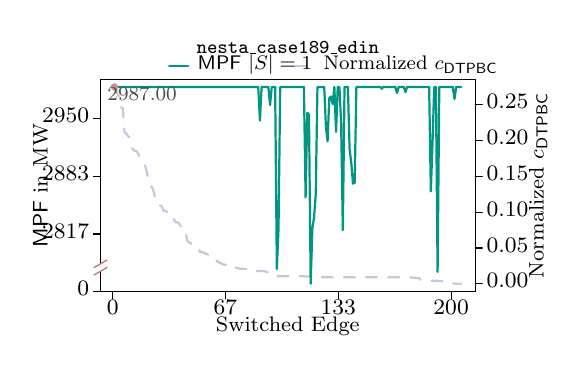
\begin{tikzpicture}[x=1pt,y=1pt]
\definecolor{fillColor}{RGB}{255,255,255}
\path[use as bounding box,fill=fillColor,fill opacity=0.00] (0,0) rectangle (440.85,271.01);
\begin{scope}
\path[clip] (  0.00,  0.00) rectangle (440.85,271.01);
\definecolor{drawColor}{RGB}{193,202,220}

\path[draw=drawColor,line width= 0.8pt,dash pattern=on 4pt off 4pt ,line join=round,line cap=round] ( 72.86,221.20) --
	( 74.28,219.64) --
	( 75.71,214.80) --
	( 77.13,213.44) --
	( 78.55,204.03) --
	( 79.97,203.22) --
	( 81.39,183.11) --
	( 82.82,182.20) --
	( 84.24,179.93) --
	( 85.66,178.78) --
	( 87.08,172.14) --
	( 88.50,168.55) --
	( 89.93,167.66) --
	( 91.35,167.32) --
	( 92.77,165.24) --
	( 94.19,162.46) --
	( 95.61,158.87) --
	( 97.04,156.96) --
	( 98.46,155.47) --
	( 99.88,151.02) --
	(101.30,142.77) --
	(102.72,138.69) --
	(104.15,137.47) --
	(105.57,134.36) --
	(106.99,128.40) --
	(108.41,128.20) --
	(109.83,124.05) --
	(111.26,121.46) --
	(112.68,121.02) --
	(114.10,117.21) --
	(115.52,116.99) --
	(116.95,116.42) --
	(118.37,116.35) --
	(119.79,111.79) --
	(121.21,111.41) --
	(122.63,110.66) --
	(124.06,107.73) --
	(125.48,107.44) --
	(126.90,106.94) --
	(128.32,104.69) --
	(129.74,102.20) --
	(131.17,102.04) --
	(132.59,100.57) --
	(134.01, 92.19) --
	(135.43, 90.58) --
	(136.85, 90.14) --
	(138.28, 87.30) --
	(139.70, 87.10) --
	(141.12, 84.80) --
	(142.54, 84.37) --
	(143.96, 84.12) --
	(145.39, 82.22) --
	(146.81, 82.22) --
	(148.23, 82.02) --
	(149.65, 80.87) --
	(151.08, 80.87) --
	(152.50, 78.23) --
	(153.92, 77.08) --
	(155.34, 77.08) --
	(156.76, 77.08) --
	(158.19, 76.23) --
	(159.61, 74.23) --
	(161.03, 73.67) --
	(162.45, 73.01) --
	(163.87, 72.15) --
	(165.30, 71.86) --
	(166.72, 71.86) --
	(168.14, 71.86) --
	(169.56, 71.86) --
	(170.98, 71.86) --
	(172.41, 71.86) --
	(173.83, 71.73) --
	(175.25, 69.14) --
	(176.67, 68.88) --
	(178.09, 68.48) --
	(179.52, 68.48) --
	(180.94, 68.48) --
	(182.36, 68.32) --
	(183.78, 68.14) --
	(185.20, 68.14) --
	(186.63, 67.77) --
	(188.05, 66.62) --
	(189.47, 66.58) --
	(190.89, 66.58) --
	(192.32, 66.58) --
	(193.74, 66.58) --
	(195.16, 66.58) --
	(196.58, 66.58) --
	(198.00, 66.38) --
	(199.43, 66.38) --
	(200.85, 65.58) --
	(202.27, 65.50) --
	(203.69, 63.79) --
	(205.11, 63.69) --
	(206.54, 63.23) --
	(207.96, 62.69) --
	(209.38, 62.18) --
	(210.80, 62.18) --
	(212.22, 62.18) --
	(213.65, 62.18) --
	(215.07, 62.18) --
	(216.49, 62.18) --
	(217.91, 62.18) --
	(219.33, 62.18) --
	(220.76, 62.18) --
	(222.18, 62.18) --
	(223.60, 62.18) --
	(225.02, 62.18) --
	(226.44, 62.18) --
	(227.87, 62.18) --
	(229.29, 62.18) --
	(230.71, 62.18) --
	(232.13, 62.15) --
	(233.56, 61.98) --
	(234.98, 61.98) --
	(236.40, 61.98) --
	(237.82, 61.98) --
	(239.24, 61.98) --
	(240.67, 61.98) --
	(242.09, 61.98) --
	(243.51, 61.71) --
	(244.93, 61.64) --
	(246.35, 61.54) --
	(247.78, 61.37) --
	(249.20, 61.30) --
	(250.62, 61.23) --
	(252.04, 61.23) --
	(253.46, 61.23) --
	(254.89, 61.23) --
	(256.31, 61.23) --
	(257.73, 61.23) --
	(259.15, 61.23) --
	(260.57, 61.23) --
	(262.00, 61.23) --
	(263.42, 61.23) --
	(264.84, 61.23) --
	(266.26, 61.23) --
	(267.69, 61.23) --
	(269.11, 61.23) --
	(270.53, 61.23) --
	(271.95, 61.23) --
	(273.37, 61.23) --
	(274.80, 61.23) --
	(276.22, 61.23) --
	(277.64, 61.23) --
	(279.06, 61.23) --
	(280.48, 61.23) --
	(281.91, 61.23) --
	(283.33, 61.23) --
	(284.75, 61.23) --
	(286.17, 61.23) --
	(287.59, 61.23) --
	(289.02, 61.23) --
	(290.44, 61.23) --
	(291.86, 61.23) --
	(293.28, 61.23) --
	(294.70, 61.23) --
	(296.13, 61.23) --
	(297.55, 61.23) --
	(298.97, 61.23) --
	(300.39, 61.23) --
	(301.81, 61.23) --
	(303.24, 61.23) --
	(304.66, 61.23) --
	(306.08, 61.23) --
	(307.50, 61.23) --
	(308.93, 61.23) --
	(310.35, 61.23) --
	(311.77, 61.23) --
	(313.19, 61.23) --
	(314.61, 61.23) --
	(316.04, 61.23) --
	(317.46, 61.23) --
	(318.88, 61.23) --
	(320.30, 61.16) --
	(321.72, 61.10) --
	(323.15, 61.03) --
	(324.57, 60.79) --
	(325.99, 60.78) --
	(327.41, 60.62) --
	(328.83, 60.62) --
	(330.26, 59.05) --
	(331.68, 58.59) --
	(333.10, 58.47) --
	(334.52, 58.46) --
	(335.94, 58.42) --
	(337.37, 58.32) --
	(338.79, 58.32) --
	(340.21, 58.32) --
	(341.63, 58.32) --
	(343.05, 58.32) --
	(344.48, 58.32) --
	(345.90, 58.17) --
	(347.32, 58.02) --
	(348.74, 58.02) --
	(350.17, 58.02) --
	(351.59, 58.02) --
	(353.01, 56.73) --
	(354.43, 56.29) --
	(355.85, 56.26) --
	(357.28, 56.02) --
	(358.70, 56.02) --
	(360.12, 55.82) --
	(361.54, 55.82) --
	(362.96, 55.82) --
	(364.39, 55.82);
\end{scope}
\begin{scope}
\path[clip] (  0.00,  0.00) rectangle (440.85,271.01);
\definecolor{drawColor}{RGB}{0,0,0}

\path[draw=drawColor,line width= 0.4pt,line join=round,line cap=round] ( 61.20, 49.20) --
	(376.05, 49.20) --
	(376.05,227.81) --
	( 61.20,227.81) --
	( 61.20, 49.20);
\end{scope}
\begin{scope}
\path[clip] (  0.00,  0.00) rectangle (440.85,271.01);
\definecolor{drawColor}{RGB}{0,0,0}

\path[draw=drawColor,line width= 0.4pt,line join=round,line cap=round] (376.05, 55.82) -- (376.05,206.18);

\path[draw=drawColor,line width= 0.4pt,line join=round,line cap=round] (376.05, 55.82) -- (382.05, 55.82);

\path[draw=drawColor,line width= 0.4pt,line join=round,line cap=round] (376.05, 85.89) -- (382.05, 85.89);

\path[draw=drawColor,line width= 0.4pt,line join=round,line cap=round] (376.05,115.96) -- (382.05,115.96);

\path[draw=drawColor,line width= 0.4pt,line join=round,line cap=round] (376.05,146.04) -- (382.05,146.04);

\path[draw=drawColor,line width= 0.4pt,line join=round,line cap=round] (376.05,176.11) -- (382.05,176.11);

\path[draw=drawColor,line width= 0.4pt,line join=round,line cap=round] (376.05,206.18) -- (382.05,206.18);

\node[text=drawColor,anchor=base west,inner sep=0pt, outer sep=0pt, scale=  1.00] at (385.65, 52.37) {0.00};

\node[text=drawColor,anchor=base west,inner sep=0pt, outer sep=0pt, scale=  1.00] at (385.65, 82.45) {0.05};

\node[text=drawColor,anchor=base west,inner sep=0pt, outer sep=0pt, scale=  1.00] at (385.65,112.52) {0.10};

\node[text=drawColor,anchor=base west,inner sep=0pt, outer sep=0pt, scale=  1.00] at (385.65,142.59) {0.15};

\node[text=drawColor,anchor=base west,inner sep=0pt, outer sep=0pt, scale=  1.00] at (385.65,172.67) {0.20};

\node[text=drawColor,anchor=base west,inner sep=0pt, outer sep=0pt, scale=  1.00] at (385.65,202.74) {0.25};
\end{scope}
\begin{scope}
\path[clip] (  0.00,  0.00) rectangle (440.85,271.01);
\definecolor{drawColor}{RGB}{0,150,130}

\path[draw=drawColor,line width= 0.8pt,line join=round,line cap=round] (118.89,238.60) -- (134.91,238.60);
\definecolor{drawColor}{RGB}{193,202,220}

\path[draw=drawColor,line width= 0.8pt,dash pattern=on 4pt off 4pt ,line join=round,line cap=round] (224.63,238.60) -- (240.65,238.60);
\definecolor{drawColor}{RGB}{0,0,0}

\node[text=drawColor,anchor=base,inner sep=0pt, outer sep=0pt, scale=  0.89] at (218.62,249.28) {\texttt{nesta\_case189\_edin}};

\node[text=drawColor,anchor=base west,inner sep=0pt, outer sep=0pt, scale=  0.89] at (142.92,235.54) {$\mathsf{MPF}~|S|=1$};

\node[text=drawColor,anchor=base west,inner sep=0pt, outer sep=0pt, scale=  0.89] at (248.66,235.54) {Normalized~$c_\mathsf{DTPBC}$};
\end{scope}
\begin{scope}
\path[clip] (  0.00,  0.00) rectangle (440.85,271.01);
\definecolor{drawColor}{RGB}{0,0,0}

\path[draw=drawColor,line width= 0.4pt,line join=round,line cap=round] ( 61.20, 49.29) -- ( 61.20,194.36);

\path[draw=drawColor,line width= 0.4pt,line join=round,line cap=round] ( 61.20, 49.29) -- ( 55.20, 49.29);

\path[draw=drawColor,line width= 0.4pt,line join=round,line cap=round] ( 61.20, 97.64) -- ( 55.20, 97.64);

\path[draw=drawColor,line width= 0.4pt,line join=round,line cap=round] ( 61.20,146.00) -- ( 55.20,146.00);

\path[draw=drawColor,line width= 0.4pt,line join=round,line cap=round] ( 61.20,194.36) -- ( 55.20,194.36);

\node[text=drawColor,anchor=base east,inner sep=0pt, outer sep=0pt, scale=  1.00] at ( 51.60, 45.84) {0};

\node[text=drawColor,anchor=base east,inner sep=0pt, outer sep=0pt, scale=  1.00] at ( 51.60, 94.20) {2817};

\node[text=drawColor,anchor=base east,inner sep=0pt, outer sep=0pt, scale=  1.00] at ( 51.60,142.56) {2883};

\node[text=drawColor,anchor=base east,inner sep=0pt, outer sep=0pt, scale=  1.00] at ( 51.60,190.92) {2950};
\end{scope}
\begin{scope}
\path[clip] (  0.00,  0.00) rectangle (440.85,271.01);
\definecolor{drawColor}{RGB}{255,255,255}
\definecolor{fillColor}{RGB}{255,255,255}

\path[draw=drawColor,line width= 0.4pt,line join=round,line cap=round,fill=fillColor] ( 55.69, 66.31) rectangle ( 66.71, 72.56);
\definecolor{drawColor}{RGB}{188,97,104}

\path[draw=drawColor,line width= 0.4pt,line join=round,line cap=round] ( 55.69, 63.18) -- ( 66.71, 69.44);

\path[draw=drawColor,line width= 0.4pt,line join=round,line cap=round] ( 55.69, 69.44) -- ( 66.71, 75.69);
\end{scope}
\begin{scope}
\path[clip] ( 61.20, 49.20) rectangle (376.05,227.81);
\definecolor{drawColor}{RGB}{0,150,130}

\path[draw=drawColor,line width= 0.8pt,line join=round,line cap=round] ( 72.86,221.20) --
	( 74.28,221.20) --
	( 75.71,221.20) --
	( 77.13,221.20) --
	( 78.55,221.20) --
	( 79.97,221.20) --
	( 81.39,221.20) --
	( 82.82,221.20) --
	( 84.24,221.20) --
	( 85.66,221.20) --
	( 87.08,221.20) --
	( 88.50,221.20) --
	( 89.93,221.20) --
	( 91.35,221.20) --
	( 92.77,221.20) --
	( 94.19,221.20) --
	( 95.61,221.20) --
	( 97.04,221.20) --
	( 98.46,221.20) --
	( 99.88,221.20) --
	(101.30,221.20) --
	(102.72,221.20) --
	(104.15,221.20) --
	(105.57,221.20) --
	(106.99,221.20) --
	(108.41,221.20) --
	(109.83,221.20) --
	(111.26,221.20) --
	(112.68,221.20) --
	(114.10,221.20) --
	(115.52,221.20) --
	(116.95,221.20) --
	(118.37,221.20) --
	(119.79,221.20) --
	(121.21,221.20) --
	(122.63,221.20) --
	(124.06,221.20) --
	(125.48,221.20) --
	(126.90,221.20) --
	(128.32,221.20) --
	(129.74,221.20) --
	(131.17,221.20) --
	(132.59,221.20) --
	(134.01,221.20) --
	(135.43,221.20) --
	(136.85,221.20) --
	(138.28,221.20) --
	(139.70,221.20) --
	(141.12,221.20) --
	(142.54,221.20) --
	(143.96,221.20) --
	(145.39,221.20) --
	(146.81,221.20) --
	(148.23,221.20) --
	(149.65,221.20) --
	(151.08,221.20) --
	(152.50,221.20) --
	(153.92,221.20) --
	(155.34,221.20) --
	(156.76,221.20) --
	(158.19,221.20) --
	(159.61,221.20) --
	(161.03,221.20) --
	(162.45,221.20) --
	(163.87,221.20) --
	(165.30,221.20) --
	(166.72,221.20) --
	(168.14,221.20) --
	(169.56,221.20) --
	(170.98,221.20) --
	(172.41,221.20) --
	(173.83,221.20) --
	(175.25,221.20) --
	(176.67,221.20) --
	(178.09,221.20) --
	(179.52,221.20) --
	(180.94,221.20) --
	(182.36,221.20) --
	(183.78,221.20) --
	(185.20,221.20) --
	(186.63,221.20) --
	(188.05,221.20) --
	(189.47,221.20) --
	(190.89,221.20) --
	(192.32,221.20) --
	(193.74,221.20) --
	(195.16,192.91) --
	(196.58,221.20) --
	(198.00,221.20) --
	(199.43,221.20) --
	(200.85,221.20) --
	(202.27,221.20) --
	(203.69,205.96) --
	(205.11,221.20) --
	(206.54,221.20) --
	(207.96,221.20) --
	(209.38, 68.15) --
	(210.80,102.24) --
	(212.22,221.20) --
	(213.65,221.20) --
	(215.07,221.20) --
	(216.49,221.20) --
	(217.91,221.20) --
	(219.33,221.20) --
	(220.76,221.20) --
	(222.18,221.20) --
	(223.60,221.20) --
	(225.02,221.20) --
	(226.44,221.20) --
	(227.87,221.20) --
	(229.29,221.20) --
	(230.71,221.20) --
	(232.13,221.20) --
	(233.56,128.35) --
	(234.98,199.44) --
	(236.40,197.99) --
	(237.82, 55.82) --
	(239.24,102.24) --
	(240.67,111.67) --
	(242.09,131.25) --
	(243.51,221.20) --
	(244.93,221.20) --
	(246.35,221.20) --
	(247.78,221.20) --
	(249.20,221.20) --
	(250.62,187.83) --
	(252.04,175.50) --
	(253.46,211.77) --
	(254.89,213.22) --
	(256.31,206.69) --
	(257.73,221.20) --
	(259.15,183.48) --
	(260.57,221.20) --
	(262.00,221.20) --
	(263.42,190.73) --
	(264.84,100.79) --
	(266.26,221.20) --
	(267.69,221.20) --
	(269.11,221.20) --
	(270.53,168.97) --
	(271.95,157.37) --
	(273.37,139.96) --
	(274.80,140.68) --
	(276.22,221.20) --
	(277.64,221.20) --
	(279.06,221.20) --
	(280.48,221.20) --
	(281.91,221.20) --
	(283.33,221.20) --
	(284.75,221.20) --
	(286.17,221.20) --
	(287.59,221.20) --
	(289.02,221.20) --
	(290.44,221.20) --
	(291.86,221.20) --
	(293.28,221.20) --
	(294.70,221.20) --
	(296.13,221.20) --
	(297.55,219.75) --
	(298.97,221.20) --
	(300.39,221.20) --
	(301.81,221.20) --
	(303.24,221.20) --
	(304.66,221.20) --
	(306.08,221.20) --
	(307.50,221.20) --
	(308.93,221.20) --
	(310.35,216.12) --
	(311.77,221.20) --
	(313.19,221.20) --
	(314.61,221.20) --
	(316.04,221.20) --
	(317.46,216.85) --
	(318.88,221.20) --
	(320.30,221.20) --
	(321.72,221.20) --
	(323.15,221.20) --
	(324.57,221.20) --
	(325.99,221.20) --
	(327.41,221.20) --
	(328.83,221.20) --
	(330.26,221.20) --
	(331.68,221.20) --
	(333.10,221.20) --
	(334.52,221.20) --
	(335.94,221.20) --
	(337.37,221.20) --
	(338.79,133.43) --
	(340.21,174.05) --
	(341.63,221.20) --
	(343.05,221.20) --
	(344.48, 65.81) --
	(345.90,221.20) --
	(347.32,221.20) --
	(348.74,221.20) --
	(350.17,221.20) --
	(351.59,221.20) --
	(353.01,221.20) --
	(354.43,221.20) --
	(355.85,221.20) --
	(357.28,221.20) --
	(358.70,211.12) --
	(360.12,221.20) --
	(361.54,221.20) --
	(362.96,221.20) --
	(364.39,221.20);
\end{scope}
\begin{scope}
\path[clip] ( 61.20, 49.20) rectangle (376.05,227.81);
\definecolor{fillColor}{RGB}{207,142,147}

\path[fill=fillColor] ( 72.86,221.20) circle (  3.15);
\end{scope}
\begin{scope}
\path[clip] ( 61.20, 49.20) rectangle (376.05,227.81);
\definecolor{drawColor}{gray}{0.30}

\node[text=drawColor,anchor=base,inner sep=0pt, outer sep=0pt, scale=  0.90] at ( 96.18,210.04) {2987.00};
\end{scope}
\begin{scope}
\path[clip] (  0.00,  0.00) rectangle (440.85,271.01);
\definecolor{drawColor}{RGB}{0,0,0}

\path[draw=drawColor,line width= 0.4pt,line join=round,line cap=round] ( 71.44, 49.20) -- (355.85, 49.20);

\path[draw=drawColor,line width= 0.4pt,line join=round,line cap=round] ( 71.44, 49.20) -- ( 71.44, 43.20);

\path[draw=drawColor,line width= 0.4pt,line join=round,line cap=round] (166.24, 49.20) -- (166.24, 43.20);

\path[draw=drawColor,line width= 0.4pt,line join=round,line cap=round] (261.05, 49.20) -- (261.05, 43.20);

\path[draw=drawColor,line width= 0.4pt,line join=round,line cap=round] (355.85, 49.20) -- (355.85, 43.20);

\node[text=drawColor,anchor=base,inner sep=0pt, outer sep=0pt, scale=  1.00] at ( 71.44, 30.00) {0};

\node[text=drawColor,anchor=base,inner sep=0pt, outer sep=0pt, scale=  1.00] at (166.24, 30.00) {67};

\node[text=drawColor,anchor=base,inner sep=0pt, outer sep=0pt, scale=  1.00] at (261.05, 30.00) {133};

\node[text=drawColor,anchor=base,inner sep=0pt, outer sep=0pt, scale=  1.00] at (355.85, 30.00) {200};

\node[text=drawColor,anchor=base,inner sep=0pt, outer sep=0pt, scale=  0.95] at (218.62, 15.60) {Switched Edge};

\node[text=drawColor,rotate= 90.00,anchor=base,inner sep=0pt, outer sep=0pt, scale=  0.95] at ( 16.80,138.51) {$\mathsf{MPF}$ in~$\mathrm{MW}$};

\node[text=drawColor,rotate= 90.00,anchor=base,inner sep=0pt, outer sep=0pt, scale=  0.95] at (433.65,138.51) {Normalized~$c_\mathsf{DTPBC}$};
\end{scope}
\end{tikzpicture}
%
    \label{plot:SwitchingBetweenness_nesta_case189_edin_dtpbc_mpf_cutY}%
  \end{subfigure}%
  
  %
  \begin{subfigure}[t]{.5\textwidth}%
    \centering%
    % Created by tikzDevice version 0.10.1 on 2018-01-31 10:28:14
% !TEX encoding = UTF-8 Unicode
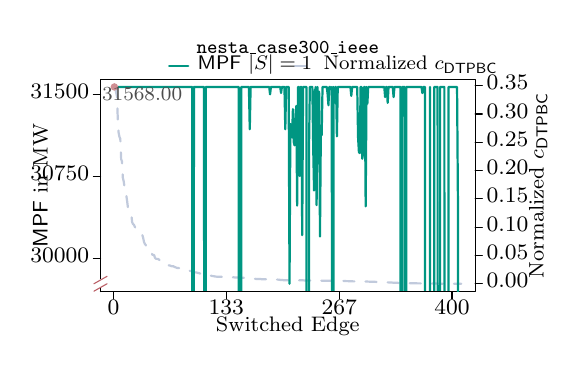
\begin{tikzpicture}[x=1pt,y=1pt]
\definecolor{fillColor}{RGB}{255,255,255}
\path[use as bounding box,fill=fillColor,fill opacity=0.00] (0,0) rectangle (440.85,271.01);
\begin{scope}
\path[clip] (  0.00,  0.00) rectangle (440.85,271.01);
\definecolor{drawColor}{RGB}{193,202,220}

\path[draw=drawColor,line width= 0.8pt,dash pattern=on 4pt off 4pt ,line join=round,line cap=round] ( 72.86,221.20) --
	( 73.57,220.72) --
	( 74.28,216.76) --
	( 74.99,213.61) --
	( 75.71,195.03) --
	( 76.42,182.75) --
	( 77.13,179.19) --
	( 77.84,177.69) --
	( 78.55,160.56) --
	( 79.26,158.58) --
	( 79.97,144.87) --
	( 80.68,142.01) --
	( 81.39,136.94) --
	( 82.10,134.07) --
	( 82.82,130.58) --
	( 83.53,125.58) --
	( 84.24,119.91) --
	( 84.95,118.14) --
	( 85.66,116.52) --
	( 86.37,115.61) --
	( 87.08,114.11) --
	( 87.79,107.66) --
	( 88.50,105.95) --
	( 89.21,105.50) --
	( 89.93,103.98) --
	( 90.64,102.48) --
	( 91.35,101.01) --
	( 92.06,100.44) --
	( 92.77, 99.77) --
	( 93.48, 99.51) --
	( 94.19, 98.46) --
	( 94.90, 97.28) --
	( 95.61, 96.89) --
	( 96.33, 96.78) --
	( 97.04, 94.43) --
	( 97.75, 90.97) --
	( 98.46, 89.31) --
	( 99.17, 88.42) --
	( 99.88, 85.95) --
	(100.59, 85.12) --
	(101.30, 85.02) --
	(102.01, 83.46) --
	(102.72, 83.02) --
	(103.44, 82.81) --
	(104.15, 81.65) --
	(104.86, 80.09) --
	(105.57, 80.05) --
	(106.28, 79.87) --
	(106.99, 77.60) --
	(107.70, 76.86) --
	(108.41, 76.71) --
	(109.12, 76.64) --
	(109.83, 76.60) --
	(110.55, 75.90) --
	(111.26, 74.98) --
	(111.97, 74.85) --
	(112.68, 74.44) --
	(113.39, 74.16) --
	(114.10, 74.07) --
	(114.81, 74.05) --
	(115.52, 73.70) --
	(116.23, 73.18) --
	(116.95, 73.10) --
	(117.66, 72.36) --
	(118.37, 71.33) --
	(119.08, 71.19) --
	(119.79, 71.10) --
	(120.50, 70.64) --
	(121.21, 70.58) --
	(121.92, 70.52) --
	(122.63, 70.46) --
	(123.34, 69.94) --
	(124.06, 69.71) --
	(124.77, 69.41) --
	(125.48, 69.14) --
	(126.19, 69.04) --
	(126.90, 68.96) --
	(127.61, 68.90) --
	(128.32, 68.54) --
	(129.03, 68.40) --
	(129.74, 68.28) --
	(130.45, 68.28) --
	(131.17, 67.75) --
	(131.88, 67.57) --
	(132.59, 67.30) --
	(133.30, 67.04) --
	(134.01, 66.91) --
	(134.72, 66.91) --
	(135.43, 66.77) --
	(136.14, 66.66) --
	(136.85, 66.58) --
	(137.57, 66.51) --
	(138.28, 66.49) --
	(138.99, 66.16) --
	(139.70, 65.87) --
	(140.41, 65.39) --
	(141.12, 65.38) --
	(141.83, 65.27) --
	(142.54, 65.05) --
	(143.25, 64.82) --
	(143.96, 64.79) --
	(144.68, 64.39) --
	(145.39, 64.37) --
	(146.10, 64.14) --
	(146.81, 63.86) --
	(147.52, 63.85) --
	(148.23, 63.85) --
	(148.94, 63.60) --
	(149.65, 63.29) --
	(150.36, 63.27) --
	(151.08, 63.24) --
	(151.79, 63.24) --
	(152.50, 62.95) --
	(153.21, 62.71) --
	(153.92, 62.65) --
	(154.63, 62.43) --
	(155.34, 62.23) --
	(156.05, 62.23) --
	(156.76, 62.09) --
	(157.47, 61.90) --
	(158.19, 61.82) --
	(158.90, 61.76) --
	(159.61, 61.73) --
	(160.32, 61.71) --
	(161.03, 61.70) --
	(161.74, 61.66) --
	(162.45, 61.66) --
	(163.16, 61.61) --
	(163.87, 61.50) --
	(164.58, 61.49) --
	(165.30, 61.44) --
	(166.01, 61.44) --
	(166.72, 61.44) --
	(167.43, 61.39) --
	(168.14, 61.37) --
	(168.85, 61.36) --
	(169.56, 61.35) --
	(170.27, 61.33) --
	(170.98, 61.32) --
	(171.70, 61.23) --
	(172.41, 61.21) --
	(173.12, 61.20) --
	(173.83, 61.15) --
	(174.54, 61.06) --
	(175.25, 61.04) --
	(175.96, 61.03) --
	(176.67, 61.02) --
	(177.38, 61.02) --
	(178.09, 61.02) --
	(178.81, 61.02) --
	(179.52, 60.98) --
	(180.23, 60.94) --
	(180.94, 60.83) --
	(181.65, 60.80) --
	(182.36, 60.77) --
	(183.07, 60.71) --
	(183.78, 60.63) --
	(184.49, 60.60) --
	(185.20, 60.59) --
	(185.92, 60.54) --
	(186.63, 60.46) --
	(187.34, 60.41) --
	(188.05, 60.39) --
	(188.76, 60.18) --
	(189.47, 60.12) --
	(190.18, 60.09) --
	(190.89, 59.98) --
	(191.60, 59.90) --
	(192.32, 59.81) --
	(193.03, 59.79) --
	(193.74, 59.77) --
	(194.45, 59.75) --
	(195.16, 59.75) --
	(195.87, 59.74) --
	(196.58, 59.63) --
	(197.29, 59.60) --
	(198.00, 59.60) --
	(198.71, 59.60) --
	(199.43, 59.59) --
	(200.14, 59.59) --
	(200.85, 59.57) --
	(201.56, 59.57) --
	(202.27, 59.55) --
	(202.98, 59.54) --
	(203.69, 59.53) --
	(204.40, 59.51) --
	(205.11, 59.48) --
	(205.82, 59.48) --
	(206.54, 59.45) --
	(207.25, 59.45) --
	(207.96, 59.41) --
	(208.67, 59.41) --
	(209.38, 59.35) --
	(210.09, 59.29) --
	(210.80, 59.26) --
	(211.51, 59.24) --
	(212.22, 58.97) --
	(212.94, 58.96) --
	(213.65, 58.95) --
	(214.36, 58.91) --
	(215.07, 58.78) --
	(215.78, 58.77) --
	(216.49, 58.74) --
	(217.20, 58.74) --
	(217.91, 58.74) --
	(218.62, 58.74) --
	(219.33, 58.74) --
	(220.05, 58.74) --
	(220.76, 58.74) --
	(221.47, 58.74) --
	(222.18, 58.74) --
	(222.89, 58.74) --
	(223.60, 58.74) --
	(224.31, 58.74) --
	(225.02, 58.74) --
	(225.73, 58.74) --
	(226.44, 58.73) --
	(227.16, 58.72) --
	(227.87, 58.72) --
	(228.58, 58.72) --
	(229.29, 58.72) --
	(230.00, 58.72) --
	(230.71, 58.69) --
	(231.42, 58.67) --
	(232.13, 58.63) --
	(232.84, 58.62) --
	(233.56, 58.60) --
	(234.27, 58.59) --
	(234.98, 58.57) --
	(235.69, 58.57) --
	(236.40, 58.55) --
	(237.11, 58.54) --
	(237.82, 58.53) --
	(238.53, 58.52) --
	(239.24, 58.52) --
	(239.95, 58.51) --
	(240.67, 58.51) --
	(241.38, 58.50) --
	(242.09, 58.49) --
	(242.80, 58.48) --
	(243.51, 58.46) --
	(244.22, 58.45) --
	(244.93, 58.43) --
	(245.64, 58.43) --
	(246.35, 58.43) --
	(247.06, 58.42) --
	(247.78, 58.42) --
	(248.49, 58.42) --
	(249.20, 58.42) --
	(249.91, 58.42) --
	(250.62, 58.42) --
	(251.33, 58.42) --
	(252.04, 58.42) --
	(252.75, 58.42) --
	(253.46, 58.42) --
	(254.18, 58.42) --
	(254.89, 58.42) --
	(255.60, 58.42) --
	(256.31, 58.42) --
	(257.02, 58.39) --
	(257.73, 58.38) --
	(258.44, 58.34) --
	(259.15, 58.31) --
	(259.86, 58.28) --
	(260.57, 58.26) --
	(261.29, 58.25) --
	(262.00, 58.24) --
	(262.71, 58.21) --
	(263.42, 58.20) --
	(264.13, 58.18) --
	(264.84, 58.17) --
	(265.55, 58.15) --
	(266.26, 58.07) --
	(266.97, 58.07) --
	(267.69, 58.02) --
	(268.40, 58.01) --
	(269.11, 58.01) --
	(269.82, 57.98) --
	(270.53, 57.97) --
	(271.24, 57.97) --
	(271.95, 57.94) --
	(272.66, 57.92) --
	(273.37, 57.81) --
	(274.08, 57.81) --
	(274.80, 57.81) --
	(275.51, 57.80) --
	(276.22, 57.79) --
	(276.93, 57.76) --
	(277.64, 57.74) --
	(278.35, 57.71) --
	(279.06, 57.71) --
	(279.77, 57.70) --
	(280.48, 57.70) --
	(281.19, 57.70) --
	(281.91, 57.70) --
	(282.62, 57.69) --
	(283.33, 57.69) --
	(284.04, 57.65) --
	(284.75, 57.63) --
	(285.46, 57.63) --
	(286.17, 57.59) --
	(286.88, 57.59) --
	(287.59, 57.54) --
	(288.31, 57.50) --
	(289.02, 57.48) --
	(289.73, 57.45) --
	(290.44, 57.44) --
	(291.15, 57.42) --
	(291.86, 57.42) --
	(292.57, 57.37) --
	(293.28, 57.35) --
	(293.99, 57.32) --
	(294.70, 57.28) --
	(295.42, 57.23) --
	(296.13, 57.17) --
	(296.84, 57.14) --
	(297.55, 57.07) --
	(298.26, 57.06) --
	(298.97, 56.99) --
	(299.68, 56.98) --
	(300.39, 56.98) --
	(301.10, 56.97) --
	(301.81, 56.97) --
	(302.53, 56.97) --
	(303.24, 56.95) --
	(303.95, 56.93) --
	(304.66, 56.84) --
	(305.37, 56.81) --
	(306.08, 56.79) --
	(306.79, 56.74) --
	(307.50, 56.73) --
	(308.21, 56.71) --
	(308.93, 56.63) --
	(309.64, 56.62) --
	(310.35, 56.61) --
	(311.06, 56.57) --
	(311.77, 56.49) --
	(312.48, 56.49) --
	(313.19, 56.46) --
	(313.90, 56.44) --
	(314.61, 56.44) --
	(315.32, 56.41) --
	(316.04, 56.39) --
	(316.75, 56.37) --
	(317.46, 56.36) --
	(318.17, 56.35) --
	(318.88, 56.34) --
	(319.59, 56.32) --
	(320.30, 56.30) --
	(321.01, 56.28) --
	(321.72, 56.25) --
	(322.43, 56.24) --
	(323.15, 56.22) --
	(323.86, 56.21) --
	(324.57, 56.19) --
	(325.28, 56.18) --
	(325.99, 56.17) --
	(326.70, 56.15) --
	(327.41, 56.14) --
	(328.12, 56.14) --
	(328.83, 56.14) --
	(329.55, 56.13) --
	(330.26, 56.11) --
	(330.97, 56.06) --
	(331.68, 56.05) --
	(332.39, 56.03) --
	(333.10, 56.03) --
	(333.81, 55.99) --
	(334.52, 55.97) --
	(335.23, 55.97) --
	(335.94, 55.97) --
	(336.66, 55.97) --
	(337.37, 55.97) --
	(338.08, 55.97) --
	(338.79, 55.97) --
	(339.50, 55.97) --
	(340.21, 55.97) --
	(340.92, 55.97) --
	(341.63, 55.97) --
	(342.34, 55.94) --
	(343.05, 55.94) --
	(343.77, 55.93) --
	(344.48, 55.93) --
	(345.19, 55.93) --
	(345.90, 55.91) --
	(346.61, 55.91) --
	(347.32, 55.90) --
	(348.03, 55.89) --
	(348.74, 55.88) --
	(349.45, 55.88) --
	(350.17, 55.87) --
	(350.88, 55.87) --
	(351.59, 55.87) --
	(352.30, 55.87) --
	(353.01, 55.87) --
	(353.72, 55.86) --
	(354.43, 55.86) --
	(355.14, 55.85) --
	(355.85, 55.84) --
	(356.56, 55.83) --
	(357.28, 55.83) --
	(357.99, 55.83) --
	(358.70, 55.83) --
	(359.41, 55.83) --
	(360.12, 55.83) --
	(360.83, 55.82) --
	(361.54, 55.82) --
	(362.25, 55.80) --
	(362.96, 55.80) --
	(363.67, 55.80) --
	(364.39, 55.80);
\end{scope}
\begin{scope}
\path[clip] (  0.00,  0.00) rectangle (440.85,271.01);
\definecolor{drawColor}{RGB}{0,0,0}

\path[draw=drawColor,line width= 0.4pt,line join=round,line cap=round] ( 61.20, 49.20) --
	(376.05, 49.20) --
	(376.05,227.81) --
	( 61.20,227.81) --
	( 61.20, 49.20);
\end{scope}
\begin{scope}
\path[clip] (  0.00,  0.00) rectangle (440.85,271.01);
\definecolor{drawColor}{RGB}{0,0,0}

\path[draw=drawColor,line width= 0.4pt,line join=round,line cap=round] (376.05, 55.80) -- (376.05,222.28);

\path[draw=drawColor,line width= 0.4pt,line join=round,line cap=round] (376.05, 55.80) -- (382.05, 55.80);

\path[draw=drawColor,line width= 0.4pt,line join=round,line cap=round] (376.05, 79.59) -- (382.05, 79.59);

\path[draw=drawColor,line width= 0.4pt,line join=round,line cap=round] (376.05,103.37) -- (382.05,103.37);

\path[draw=drawColor,line width= 0.4pt,line join=round,line cap=round] (376.05,127.15) -- (382.05,127.15);

\path[draw=drawColor,line width= 0.4pt,line join=round,line cap=round] (376.05,150.93) -- (382.05,150.93);

\path[draw=drawColor,line width= 0.4pt,line join=round,line cap=round] (376.05,174.71) -- (382.05,174.71);

\path[draw=drawColor,line width= 0.4pt,line join=round,line cap=round] (376.05,198.50) -- (382.05,198.50);

\path[draw=drawColor,line width= 0.4pt,line join=round,line cap=round] (376.05,222.28) -- (382.05,222.28);

\node[text=drawColor,anchor=base west,inner sep=0pt, outer sep=0pt, scale=  1.00] at (385.65, 52.36) {0.00};

\node[text=drawColor,anchor=base west,inner sep=0pt, outer sep=0pt, scale=  1.00] at (385.65, 76.14) {0.05};

\node[text=drawColor,anchor=base west,inner sep=0pt, outer sep=0pt, scale=  1.00] at (385.65, 99.93) {0.10};

\node[text=drawColor,anchor=base west,inner sep=0pt, outer sep=0pt, scale=  1.00] at (385.65,123.71) {0.15};

\node[text=drawColor,anchor=base west,inner sep=0pt, outer sep=0pt, scale=  1.00] at (385.65,147.49) {0.20};

\node[text=drawColor,anchor=base west,inner sep=0pt, outer sep=0pt, scale=  1.00] at (385.65,171.27) {0.25};

\node[text=drawColor,anchor=base west,inner sep=0pt, outer sep=0pt, scale=  1.00] at (385.65,195.05) {0.30};

\node[text=drawColor,anchor=base west,inner sep=0pt, outer sep=0pt, scale=  1.00] at (385.65,218.84) {0.35};
\end{scope}
\begin{scope}
\path[clip] (  0.00,  0.00) rectangle (440.85,271.01);
\definecolor{drawColor}{RGB}{0,150,130}

\path[draw=drawColor,line width= 0.8pt,line join=round,line cap=round] (118.89,238.60) -- (134.91,238.60);
\definecolor{drawColor}{RGB}{193,202,220}

\path[draw=drawColor,line width= 0.8pt,dash pattern=on 4pt off 4pt ,line join=round,line cap=round] (224.63,238.60) -- (240.65,238.60);
\definecolor{drawColor}{RGB}{0,0,0}

\node[text=drawColor,anchor=base,inner sep=0pt, outer sep=0pt, scale=  0.89] at (218.62,249.28) {\texttt{nesta\_case300\_ieee}};

\node[text=drawColor,anchor=base west,inner sep=0pt, outer sep=0pt, scale=  0.89] at (142.92,235.54) {$\mathsf{MPF}~|S|=1$};

\node[text=drawColor,anchor=base west,inner sep=0pt, outer sep=0pt, scale=  0.89] at (248.66,235.54) {Normalized~$c_\mathsf{DTPBC}$};
\end{scope}
\begin{scope}
\path[clip] (  0.00,  0.00) rectangle (440.85,271.01);
\definecolor{drawColor}{RGB}{0,0,0}

\path[draw=drawColor,line width= 0.4pt,line join=round,line cap=round] ( 61.20, 76.97) -- ( 61.20,214.94);

\path[draw=drawColor,line width= 0.4pt,line join=round,line cap=round] ( 61.20, 76.97) -- ( 55.20, 76.97);

\path[draw=drawColor,line width= 0.4pt,line join=round,line cap=round] ( 61.20,145.96) -- ( 55.20,145.96);

\path[draw=drawColor,line width= 0.4pt,line join=round,line cap=round] ( 61.20,214.94) -- ( 55.20,214.94);

\node[text=drawColor,anchor=base east,inner sep=0pt, outer sep=0pt, scale=  1.00] at ( 51.60, 73.53) {30000};

\node[text=drawColor,anchor=base east,inner sep=0pt, outer sep=0pt, scale=  1.00] at ( 51.60,142.51) {30750};

\node[text=drawColor,anchor=base east,inner sep=0pt, outer sep=0pt, scale=  1.00] at ( 51.60,211.50) {31500};
\end{scope}
\begin{scope}
\path[clip] (  0.00,  0.00) rectangle (440.85,271.01);
\definecolor{drawColor}{RGB}{255,255,255}
\definecolor{fillColor}{RGB}{255,255,255}

\path[draw=drawColor,line width= 0.4pt,line join=round,line cap=round,fill=fillColor] ( 55.69, 52.69) rectangle ( 66.71, 58.94);
\definecolor{drawColor}{RGB}{188,97,104}

\path[draw=drawColor,line width= 0.4pt,line join=round,line cap=round] ( 55.69, 49.56) -- ( 66.71, 55.82);

\path[draw=drawColor,line width= 0.4pt,line join=round,line cap=round] ( 55.69, 55.82) -- ( 66.71, 62.07);
\end{scope}
\begin{scope}
\path[clip] ( 61.20, 49.20) rectangle (376.05,227.81);
\definecolor{drawColor}{RGB}{0,150,130}

\path[draw=drawColor,line width= 0.8pt,line join=round,line cap=round] ( 72.86,221.20) --
	( 73.57,221.20) --
	( 74.28,221.20) --
	( 74.99,221.20) --
	( 75.71,221.20) --
	( 76.42,221.20) --
	( 77.13,221.20) --
	( 77.84,221.20) --
	( 78.55,221.20) --
	( 79.26,221.20) --
	( 79.97,221.20) --
	( 80.68,221.20) --
	( 81.39,221.20) --
	( 82.10,221.20) --
	( 82.82,221.20) --
	( 83.53,221.20) --
	( 84.24,221.20) --
	( 84.95,221.20) --
	( 85.66,221.20) --
	( 86.37,221.20) --
	( 87.08,221.20) --
	( 87.79,221.20) --
	( 88.50,221.20) --
	( 89.21,221.20) --
	( 89.93,221.20) --
	( 90.64,221.20) --
	( 91.35,221.20) --
	( 92.06,221.20) --
	( 92.77,221.20) --
	( 93.48,221.20) --
	( 94.19,221.20) --
	( 94.90,221.20) --
	( 95.61,221.20) --
	( 96.33,221.20) --
	( 97.04,221.20) --
	( 97.75,221.20) --
	( 98.46,221.20) --
	( 99.17,221.20) --
	( 99.88,221.20) --
	(100.59,221.20) --
	(101.30,221.20) --
	(102.01,221.20) --
	(102.72,221.20) --
	(103.44,221.20) --
	(104.15,221.20) --
	(104.86,221.20) --
	(105.57,221.20) --
	(106.28,221.20) --
	(106.99,221.20) --
	(107.70,221.20) --
	(108.41,221.20) --
	(109.12,221.20) --
	(109.83,221.20) --
	(110.55,221.20) --
	(111.26,221.20) --
	(111.97,221.20) --
	(112.68,221.20) --
	(113.39,221.20) --
	(114.10,221.20) --
	(114.81,221.20) --
	(115.52,221.20) --
	(116.23,221.20) --
	(116.95,221.20) --
	(117.66,221.20) --
	(118.37,221.20) --
	(119.08,221.20) --
	(119.79,221.20) --
	(120.50,221.20) --
	(121.21,221.20) --
	(121.92,221.20) --
	(122.63,221.20) --
	(123.34,221.20) --
	(124.06,221.20) --
	(124.77,221.20) --
	(125.48,221.20) --
	(126.19,221.20) --
	(126.90,221.20) --
	(127.61,221.20) --
	(128.32,221.20) --
	(129.03,221.20) --
	(129.74,221.20) --
	(130.45,221.20) --
	(131.17,221.20) --
	(131.88,221.20) --
	(132.59,221.20) --
	(133.30,221.20) --
	(134.01,221.20) --
	(134.72,221.20) --
	(135.43,221.20) --
	(136.14,221.20) --
	(136.85,221.20) --
	(137.57,221.20) --
	(138.28,221.20) --
	(138.33,  0.00);

\path[draw=drawColor,line width= 0.8pt,line join=round,line cap=round] (139.64,  0.00) --
	(139.70,221.20) --
	(140.41,221.20) --
	(141.12,221.20) --
	(141.83,221.20) --
	(142.54,221.20) --
	(143.25,221.20) --
	(143.96,221.20) --
	(144.68,221.20) --
	(145.39,221.20) --
	(146.10,221.20) --
	(146.81,221.20) --
	(147.52,221.20) --
	(148.23,221.20) --
	(148.29,  0.00);

\path[draw=drawColor,line width= 0.8pt,line join=round,line cap=round] (149.60,  0.00) --
	(149.65,221.20) --
	(150.36,221.20) --
	(151.08,221.20) --
	(151.79,221.20) --
	(152.50,221.20) --
	(153.21,221.20) --
	(153.92,221.20) --
	(154.63,221.20) --
	(155.34,221.20) --
	(156.05,221.20) --
	(156.76,221.20) --
	(157.47,221.20) --
	(158.19,221.20) --
	(158.90,221.20) --
	(159.61,221.20) --
	(160.32,221.20) --
	(161.03,221.20) --
	(161.74,221.20) --
	(162.45,221.20) --
	(163.16,221.20) --
	(163.87,221.20) --
	(164.58,221.20) --
	(165.30,221.20) --
	(166.01,221.20) --
	(166.72,221.20) --
	(167.43,221.20) --
	(168.14,221.20) --
	(168.85,221.20) --
	(169.56,221.20) --
	(170.27,221.20) --
	(170.98,221.20) --
	(171.70,221.20) --
	(172.41,221.20) --
	(173.12,221.20) --
	(173.83,221.20) --
	(174.54,221.20) --
	(175.25,221.20) --
	(175.96,221.20) --
	(176.67,221.20) --
	(177.38,221.20) --
	(177.44,  0.00);

\path[draw=drawColor,line width= 0.8pt,line join=round,line cap=round] (179.46,  0.00) --
	(179.52,221.20) --
	(180.23,221.20) --
	(180.94,221.20) --
	(181.65,221.20) --
	(182.36,221.20) --
	(183.07,221.20) --
	(183.78,221.20) --
	(184.49,221.20) --
	(185.20,221.20) --
	(185.92,221.20) --
	(186.63,185.69) --
	(187.34,221.20) --
	(188.05,221.20) --
	(188.76,221.20) --
	(189.47,221.20) --
	(190.18,221.20) --
	(190.89,221.20) --
	(191.60,221.20) --
	(192.32,221.20) --
	(193.03,221.20) --
	(193.74,221.20) --
	(194.45,221.20) --
	(195.16,221.20) --
	(195.87,221.20) --
	(196.58,221.20) --
	(197.29,221.20) --
	(198.00,221.20) --
	(198.71,221.20) --
	(199.43,221.20) --
	(200.14,221.20) --
	(200.85,221.11) --
	(201.56,221.20) --
	(202.27,221.20) --
	(202.98,221.20) --
	(203.69,214.94) --
	(204.40,221.20) --
	(205.11,221.20) --
	(205.82,221.20) --
	(206.54,221.20) --
	(207.25,221.20) --
	(207.96,221.20) --
	(208.67,221.20) --
	(209.38,221.20) --
	(210.09,221.20) --
	(210.80,221.20) --
	(211.51,221.20) --
	(212.22,221.20) --
	(212.94,216.12) --
	(213.65,221.20) --
	(214.36,221.20) --
	(215.07,221.20) --
	(215.78,221.20) --
	(216.49,185.69) --
	(217.20,221.20) --
	(217.91,221.20) --
	(218.62,221.20) --
	(219.33,221.20) --
	(220.05, 55.82) --
	(220.76,190.11) --
	(221.47,186.06) --
	(222.18,178.79) --
	(222.89,202.62) --
	(223.60,174.93) --
	(224.31,172.08) --
	(225.02,192.87) --
	(225.73,205.19) --
	(226.44,121.49) --
	(227.16,221.20) --
	(227.87,221.20) --
	(228.58,146.32) --
	(229.29,221.20) --
	(230.00,221.20) --
	(230.71, 96.65) --
	(231.42,221.20) --
	(232.13,221.20) --
	(232.84,221.20) --
	(233.56,221.20) --
	(234.27,221.20) --
	(234.32,  0.00);

\path[draw=drawColor,line width= 0.8pt,line join=round,line cap=round] (236.36,  0.00) --
	(236.40,167.57) --
	(237.11,221.20) --
	(237.82,221.20) --
	(238.53,221.20) --
	(239.24,221.20) --
	(239.95,169.78) --
	(240.67,134.18) --
	(241.38,217.10) --
	(242.09,221.20) --
	(242.80,121.88) --
	(243.51,221.20) --
	(244.22,190.38) --
	(244.93,217.24) --
	(245.64, 95.55) --
	(246.35,181.46) --
	(247.06,180.73) --
	(247.78,221.20) --
	(248.49,221.20) --
	(249.20,221.20) --
	(249.91,221.20) --
	(250.62,221.20) --
	(251.33,221.20) --
	(252.04,215.40) --
	(252.75,205.84) --
	(253.46,221.20) --
	(254.18,221.20) --
	(254.89,219.17) --
	(255.60,221.20) --
	(255.65,  0.00);

\path[draw=drawColor,line width= 0.8pt,line join=round,line cap=round] (256.97,  0.00) --
	(257.02,221.20) --
	(257.73,207.73) --
	(258.44,221.20) --
	(259.15,221.20) --
	(259.86,179.71) --
	(260.57,221.20) --
	(261.29,221.20) --
	(262.00,221.20) --
	(262.71,221.20) --
	(263.42,221.20) --
	(264.13,221.20) --
	(264.84,221.20) --
	(265.55,221.20) --
	(266.26,221.20) --
	(266.97,221.20) --
	(267.69,221.20) --
	(268.40,221.20) --
	(269.11,221.20) --
	(269.82,221.20) --
	(270.53,221.20) --
	(271.24,221.20) --
	(271.95,213.69) --
	(272.66,221.20) --
	(273.37,221.20) --
	(274.08,221.20) --
	(274.80,221.20) --
	(275.51,221.20) --
	(276.22,221.20) --
	(276.93,221.20) --
	(277.64,179.16) --
	(278.35,166.56) --
	(279.06,165.55) --
	(279.77,221.20) --
	(280.48,221.20) --
	(281.19,160.86) --
	(281.91,165.73) --
	(282.62,221.20) --
	(283.33,221.20) --
	(284.04,120.85) --
	(284.75,221.20) --
	(285.46,207.07) --
	(286.17,221.20) --
	(286.88,221.20) --
	(287.59,221.20) --
	(288.31,221.20) --
	(289.02,221.20) --
	(289.73,221.20) --
	(290.44,221.20) --
	(291.15,221.20) --
	(291.86,221.20) --
	(292.57,221.20) --
	(293.28,221.20) --
	(293.99,221.20) --
	(294.70,221.20) --
	(295.42,221.20) --
	(296.13,221.20) --
	(296.84,221.20) --
	(297.55,221.20) --
	(298.26,220.99) --
	(298.97,221.20) --
	(299.68,221.20) --
	(300.39,212.69) --
	(301.10,221.20) --
	(301.81,221.20) --
	(302.53,207.83) --
	(303.24,221.20) --
	(303.95,221.20) --
	(304.66,221.20) --
	(305.37,221.20) --
	(306.08,221.20) --
	(306.79,221.20) --
	(307.50,212.64) --
	(308.21,221.20) --
	(308.93,221.20) --
	(309.64,221.20) --
	(310.35,221.20) --
	(311.06,221.20) --
	(311.77,221.20) --
	(312.48,221.20) --
	(313.19,221.20) --
	(313.25,  0.00);

\path[draw=drawColor,line width= 0.8pt,line join=round,line cap=round] (314.56,  0.00) --
	(314.61,221.20) --
	(315.32,221.20) --
	(316.04,221.20) --
	(316.75,221.20) --
	(316.80,  0.00);

\path[draw=drawColor,line width= 0.8pt,line join=round,line cap=round] (318.11,  0.00) --
	(318.17,221.20) --
	(318.88,221.20) --
	(319.59,221.20) --
	(320.30,221.20) --
	(321.01,221.20) --
	(321.72,221.20) --
	(322.43,221.20) --
	(323.15,221.20) --
	(323.86,221.20) --
	(324.57,221.20) --
	(325.28,221.20) --
	(325.99,221.20) --
	(326.70,221.20) --
	(327.41,221.20) --
	(328.12,221.20) --
	(328.83,221.20) --
	(329.55,221.20) --
	(330.26,221.20) --
	(330.97,221.20) --
	(331.68,216.00) --
	(332.39,221.20) --
	(333.10,221.20) --
	(333.81,221.20) --
	(333.87,  0.00);

\path[draw=drawColor,line width= 0.8pt,line join=round,line cap=round] (338.02,  0.00) --
	(338.08,221.20) --
	(338.13,  0.00);

\path[draw=drawColor,line width= 0.8pt,line join=round,line cap=round] (341.58,  0.00) --
	(341.63,221.20) --
	(342.34,221.20) --
	(343.05,221.20) --
	(343.77,221.20) --
	(344.48,221.20) --
	(344.53,  0.00);

\path[draw=drawColor,line width= 0.8pt,line join=round,line cap=round] (346.56,  0.00) --
	(346.61,221.20) --
	(347.32,221.20) --
	(348.03,221.20) --
	(348.74,221.20) --
	(349.45,221.20) --
	(350.17,221.20) --
	(350.22,  0.00);

\path[draw=drawColor,line width= 0.8pt,line join=round,line cap=round] (353.67,  0.00) --
	(353.72,221.20) --
	(354.43,221.20) --
	(355.14,221.20) --
	(355.85,221.20) --
	(356.56,221.20) --
	(357.28,221.20) --
	(357.99,221.20) --
	(358.70,221.20) --
	(359.41,221.20) --
	(360.12,221.20) --
	(360.83,221.20) --
	(361.54,129.01) --
	(361.57,  0.00);
\end{scope}
\begin{scope}
\path[clip] ( 61.20, 49.20) rectangle (376.05,227.81);
\definecolor{fillColor}{RGB}{207,142,147}

\path[fill=fillColor] ( 72.86,221.20) circle (  3.15);
\end{scope}
\begin{scope}
\path[clip] ( 61.20, 49.20) rectangle (376.05,227.81);
\definecolor{drawColor}{gray}{0.30}

\node[text=drawColor,anchor=base,inner sep=0pt, outer sep=0pt, scale=  0.90] at ( 96.18,210.04) {31568.00};
\end{scope}
\begin{scope}
\path[clip] (  0.00,  0.00) rectangle (440.85,271.01);
\definecolor{drawColor}{RGB}{0,0,0}

\path[draw=drawColor,line width= 0.4pt,line join=round,line cap=round] ( 72.15, 49.20) -- (356.56, 49.20);

\path[draw=drawColor,line width= 0.4pt,line join=round,line cap=round] ( 72.15, 49.20) -- ( 72.15, 43.20);

\path[draw=drawColor,line width= 0.4pt,line join=round,line cap=round] (166.95, 49.20) -- (166.95, 43.20);

\path[draw=drawColor,line width= 0.4pt,line join=round,line cap=round] (261.76, 49.20) -- (261.76, 43.20);

\path[draw=drawColor,line width= 0.4pt,line join=round,line cap=round] (356.56, 49.20) -- (356.56, 43.20);

\node[text=drawColor,anchor=base,inner sep=0pt, outer sep=0pt, scale=  1.00] at ( 72.15, 30.00) {0};

\node[text=drawColor,anchor=base,inner sep=0pt, outer sep=0pt, scale=  1.00] at (166.95, 30.00) {133};

\node[text=drawColor,anchor=base,inner sep=0pt, outer sep=0pt, scale=  1.00] at (261.76, 30.00) {267};

\node[text=drawColor,anchor=base,inner sep=0pt, outer sep=0pt, scale=  1.00] at (356.56, 30.00) {400};

\node[text=drawColor,anchor=base,inner sep=0pt, outer sep=0pt, scale=  0.95] at (218.62, 15.60) {Switched Edge};

\node[text=drawColor,rotate= 90.00,anchor=base,inner sep=0pt, outer sep=0pt, scale=  0.95] at ( 16.80,138.51) {$\mathsf{MPF}$ in~$\mathrm{MW}$};

\node[text=drawColor,rotate= 90.00,anchor=base,inner sep=0pt, outer sep=0pt, scale=  0.95] at (433.65,138.51) {Normalized~$c_\mathsf{DTPBC}$};
\end{scope}
\end{tikzpicture}
%
    \label{plot:SwitchingBetweenness_nesta_case300_ieee_dtpbc_mpf_cutY}%
  \end{subfigure}%
  \hfill
  %
  \begin{subfigure}[t]{.5\textwidth}%
    \centering%
    % Created by tikzDevice version 0.10.1 on 2018-01-31 10:27:32
% !TEX encoding = UTF-8 Unicode
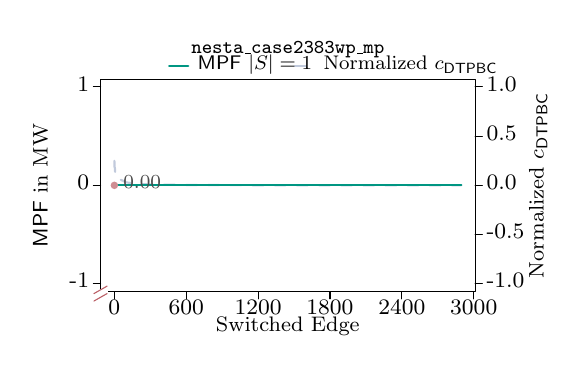
\begin{tikzpicture}[x=1pt,y=1pt]
\definecolor{fillColor}{RGB}{255,255,255}
\path[use as bounding box,fill=fillColor,fill opacity=0.00] (0,0) rectangle (440.85,271.01);
\begin{scope}
\path[clip] (  0.00,  0.00) rectangle (440.85,271.01);
\definecolor{drawColor}{RGB}{193,202,220}

\path[draw=drawColor,line width= 0.8pt,dash pattern=on 4pt off 4pt ,line join=round,line cap=round] ( 72.86,159.12) --
	( 72.96,154.95) --
	( 73.06,153.72) --
	( 73.16,153.52) --
	( 73.26,153.17) --
	( 73.36,151.64) --
	( 73.47,150.21) --
	( 73.57,149.18) --
	( 73.67,149.01) --
	( 73.77,148.97) --
	( 73.87,148.85) --
	( 73.97,148.72) --
	( 74.07,148.66) --
	( 74.17,148.62) --
	( 74.27,148.56) --
	( 74.37,148.20) --
	( 74.47,147.45) --
	( 74.57,146.58) --
	( 74.67,146.58) --
	( 74.77,146.56) --
	( 74.87,146.08) --
	( 74.98,145.85) --
	( 75.08,145.82) --
	( 75.18,145.66) --
	( 75.28,145.45) --
	( 75.38,145.35) --
	( 75.48,145.08) --
	( 75.58,144.78) --
	( 75.68,144.77) --
	( 75.78,144.50) --
	( 75.88,144.49) --
	( 75.98,144.42) --
	( 76.08,144.38) --
	( 76.18,144.36) --
	( 76.28,144.26) --
	( 76.39,144.22) --
	( 76.49,144.17) --
	( 76.59,144.14) --
	( 76.69,144.12) --
	( 76.79,144.00) --
	( 76.89,143.99) --
	( 76.99,143.95) --
	( 77.09,143.93) --
	( 77.19,143.82) --
	( 77.29,143.76) --
	( 77.39,143.68) --
	( 77.49,143.55) --
	( 77.59,143.49) --
	( 77.69,143.47) --
	( 77.80,143.45) --
	( 77.90,143.45) --
	( 78.00,143.45) --
	( 78.10,143.44) --
	( 78.20,143.40) --
	( 78.30,143.20) --
	( 78.40,143.15) --
	( 78.50,143.09) --
	( 78.60,143.00) --
	( 78.70,142.94) --
	( 78.80,142.82) --
	( 78.90,142.80) --
	( 79.00,142.73) --
	( 79.10,142.72) --
	( 79.21,142.64) --
	( 79.31,142.63) --
	( 79.41,142.62) --
	( 79.51,142.60) --
	( 79.61,142.58) --
	( 79.71,142.57) --
	( 79.81,142.53) --
	( 79.91,142.50) --
	( 80.01,142.45) --
	( 80.11,142.24) --
	( 80.21,142.24) --
	( 80.31,142.21) --
	( 80.41,142.17) --
	( 80.51,142.00) --
	( 80.61,141.93) --
	( 80.72,141.91) --
	( 80.82,141.88) --
	( 80.92,141.86) --
	( 81.02,141.86) --
	( 81.12,141.83) --
	( 81.22,141.83) --
	( 81.32,141.82) --
	( 81.42,141.80) --
	( 81.52,141.58) --
	( 81.62,141.53) --
	( 81.72,141.52) --
	( 81.82,141.38) --
	( 81.92,141.38) --
	( 82.02,141.34) --
	( 82.13,141.30) --
	( 82.23,141.28) --
	( 82.33,141.22) --
	( 82.43,141.11) --
	( 82.53,141.11) --
	( 82.63,141.10) --
	( 82.73,141.08) --
	( 82.83,141.03) --
	( 82.93,141.01) --
	( 83.03,141.00) --
	( 83.13,140.99) --
	( 83.23,140.99) --
	( 83.33,140.97) --
	( 83.43,140.96) --
	( 83.54,140.91) --
	( 83.64,140.90) --
	( 83.74,140.89) --
	( 83.84,140.87) --
	( 83.94,140.83) --
	( 84.04,140.83) --
	( 84.14,140.81) --
	( 84.24,140.80) --
	( 84.34,140.79) --
	( 84.44,140.78) --
	( 84.54,140.77) --
	( 84.64,140.74) --
	( 84.74,140.71) --
	( 84.84,140.71) --
	( 84.94,140.70) --
	( 85.05,140.68) --
	( 85.15,140.67) --
	( 85.25,140.66) --
	( 85.35,140.62) --
	( 85.45,140.60) --
	( 85.55,140.60) --
	( 85.65,140.58) --
	( 85.75,140.56) --
	( 85.85,140.55) --
	( 85.95,140.54) --
	( 86.05,140.53) --
	( 86.15,140.42) --
	( 86.25,140.40) --
	( 86.35,140.37) --
	( 86.46,140.35) --
	( 86.56,140.34) --
	( 86.66,140.33) --
	( 86.76,140.30) --
	( 86.86,140.30) --
	( 86.96,140.28) --
	( 87.06,140.24) --
	( 87.16,140.23) --
	( 87.26,140.20) --
	( 87.36,140.18) --
	( 87.46,140.17) --
	( 87.56,140.17) --
	( 87.66,140.17) --
	( 87.76,140.16) --
	( 87.87,140.14) --
	( 87.97,140.14) --
	( 88.07,140.10) --
	( 88.17,140.10) --
	( 88.27,140.10) --
	( 88.37,140.09) --
	( 88.47,140.09) --
	( 88.57,140.09) --
	( 88.67,140.06) --
	( 88.77,140.04) --
	( 88.87,140.04) --
	( 88.97,140.03) --
	( 89.07,140.03) --
	( 89.17,140.00) --
	( 89.28,139.99) --
	( 89.38,139.98) --
	( 89.48,139.97) --
	( 89.58,139.93) --
	( 89.68,139.92) --
	( 89.78,139.92) --
	( 89.88,139.90) --
	( 89.98,139.90) --
	( 90.08,139.89) --
	( 90.18,139.88) --
	( 90.28,139.88) --
	( 90.38,139.87) --
	( 90.48,139.86) --
	( 90.58,139.86) --
	( 90.68,139.85) --
	( 90.79,139.85) --
	( 90.89,139.84) --
	( 90.99,139.84) --
	( 91.09,139.84) --
	( 91.19,139.82) --
	( 91.29,139.82) --
	( 91.39,139.82) --
	( 91.49,139.81) --
	( 91.59,139.81) --
	( 91.69,139.81) --
	( 91.79,139.80) --
	( 91.89,139.79) --
	( 91.99,139.78) --
	( 92.09,139.76) --
	( 92.20,139.76) --
	( 92.30,139.76) --
	( 92.40,139.74) --
	( 92.50,139.74) --
	( 92.60,139.74) --
	( 92.70,139.73) --
	( 92.80,139.73) --
	( 92.90,139.72) --
	( 93.00,139.72) --
	( 93.10,139.72) --
	( 93.20,139.71) --
	( 93.30,139.71) --
	( 93.40,139.69) --
	( 93.50,139.69) --
	( 93.61,139.69) --
	( 93.71,139.68) --
	( 93.81,139.68) --
	( 93.91,139.68) --
	( 94.01,139.66) --
	( 94.11,139.66) --
	( 94.21,139.66) --
	( 94.31,139.64) --
	( 94.41,139.63) --
	( 94.51,139.62) --
	( 94.61,139.58) --
	( 94.71,139.57) --
	( 94.81,139.57) --
	( 94.91,139.56) --
	( 95.01,139.56) --
	( 95.12,139.55) --
	( 95.22,139.55) --
	( 95.32,139.53) --
	( 95.42,139.52) --
	( 95.52,139.52) --
	( 95.62,139.51) --
	( 95.72,139.51) --
	( 95.82,139.50) --
	( 95.92,139.50) --
	( 96.02,139.50) --
	( 96.12,139.50) --
	( 96.22,139.49) --
	( 96.32,139.49) --
	( 96.42,139.48) --
	( 96.53,139.47) --
	( 96.63,139.47) --
	( 96.73,139.46) --
	( 96.83,139.45) --
	( 96.93,139.45) --
	( 97.03,139.45) --
	( 97.13,139.44) --
	( 97.23,139.43) --
	( 97.33,139.42) --
	( 97.43,139.42) --
	( 97.53,139.41) --
	( 97.63,139.40) --
	( 97.73,139.40) --
	( 97.83,139.40) --
	( 97.94,139.40) --
	( 98.04,139.39) --
	( 98.14,139.39) --
	( 98.24,139.39) --
	( 98.34,139.39) --
	( 98.44,139.38) --
	( 98.54,139.37) --
	( 98.64,139.37) --
	( 98.74,139.37) --
	( 98.84,139.37) --
	( 98.94,139.36) --
	( 99.04,139.36) --
	( 99.14,139.36) --
	( 99.24,139.36) --
	( 99.34,139.35) --
	( 99.45,139.35) --
	( 99.55,139.35) --
	( 99.65,139.35) --
	( 99.75,139.35) --
	( 99.85,139.35) --
	( 99.95,139.34) --
	(100.05,139.34) --
	(100.15,139.34) --
	(100.25,139.33) --
	(100.35,139.33) --
	(100.45,139.33) --
	(100.55,139.31) --
	(100.65,139.31) --
	(100.75,139.31) --
	(100.86,139.31) --
	(100.96,139.30) --
	(101.06,139.30) --
	(101.16,139.30) --
	(101.26,139.30) --
	(101.36,139.29) --
	(101.46,139.29) --
	(101.56,139.29) --
	(101.66,139.29) --
	(101.76,139.29) --
	(101.86,139.28) --
	(101.96,139.28) --
	(102.06,139.28) --
	(102.16,139.27) --
	(102.27,139.27) --
	(102.37,139.26) --
	(102.47,139.26) --
	(102.57,139.26) --
	(102.67,139.25) --
	(102.77,139.25) --
	(102.87,139.25) --
	(102.97,139.25) --
	(103.07,139.25) --
	(103.17,139.24) --
	(103.27,139.24) --
	(103.37,139.24) --
	(103.47,139.24) --
	(103.57,139.24) --
	(103.68,139.24) --
	(103.78,139.24) --
	(103.88,139.24) --
	(103.98,139.24) --
	(104.08,139.23) --
	(104.18,139.23) --
	(104.28,139.23) --
	(104.38,139.23) --
	(104.48,139.22) --
	(104.58,139.22) --
	(104.68,139.22) --
	(104.78,139.22) --
	(104.88,139.22) --
	(104.98,139.21) --
	(105.08,139.21) --
	(105.19,139.21) --
	(105.29,139.21) --
	(105.39,139.21) --
	(105.49,139.21) --
	(105.59,139.21) --
	(105.69,139.20) --
	(105.79,139.20) --
	(105.89,139.20) --
	(105.99,139.20) --
	(106.09,139.20) --
	(106.19,139.20) --
	(106.29,139.20) --
	(106.39,139.20) --
	(106.49,139.19) --
	(106.60,139.19) --
	(106.70,139.19) --
	(106.80,139.18) --
	(106.90,139.18) --
	(107.00,139.18) --
	(107.10,139.18) --
	(107.20,139.18) --
	(107.30,139.17) --
	(107.40,139.17) --
	(107.50,139.17) --
	(107.60,139.17) --
	(107.70,139.16) --
	(107.80,139.16) --
	(107.90,139.16) --
	(108.01,139.16) --
	(108.11,139.16) --
	(108.21,139.16) --
	(108.31,139.15) --
	(108.41,139.15) --
	(108.51,139.15) --
	(108.61,139.15) --
	(108.71,139.15) --
	(108.81,139.15) --
	(108.91,139.15) --
	(109.01,139.15) --
	(109.11,139.15) --
	(109.21,139.14) --
	(109.31,139.14) --
	(109.41,139.14) --
	(109.52,139.14) --
	(109.62,139.13) --
	(109.72,139.13) --
	(109.82,139.13) --
	(109.92,139.13) --
	(110.02,139.13) --
	(110.12,139.13) --
	(110.22,139.13) --
	(110.32,139.13) --
	(110.42,139.12) --
	(110.52,139.12) --
	(110.62,139.12) --
	(110.72,139.12) --
	(110.82,139.12) --
	(110.93,139.12) --
	(111.03,139.12) --
	(111.13,139.12) --
	(111.23,139.12) --
	(111.33,139.12) --
	(111.43,139.12) --
	(111.53,139.11) --
	(111.63,139.11) --
	(111.73,139.11) --
	(111.83,139.11) --
	(111.93,139.11) --
	(112.03,139.11) --
	(112.13,139.11) --
	(112.23,139.10) --
	(112.34,139.10) --
	(112.44,139.10) --
	(112.54,139.10) --
	(112.64,139.09) --
	(112.74,139.09) --
	(112.84,139.09) --
	(112.94,139.09) --
	(113.04,139.09) --
	(113.14,139.09) --
	(113.24,139.09) --
	(113.34,139.09) --
	(113.44,139.09) --
	(113.54,139.08) --
	(113.64,139.08) --
	(113.74,139.08) --
	(113.85,139.08) --
	(113.95,139.08) --
	(114.05,139.08) --
	(114.15,139.08) --
	(114.25,139.08) --
	(114.35,139.08) --
	(114.45,139.07) --
	(114.55,139.07) --
	(114.65,139.07) --
	(114.75,139.07) --
	(114.85,139.07) --
	(114.95,139.06) --
	(115.05,139.06) --
	(115.15,139.06) --
	(115.26,139.06) --
	(115.36,139.06) --
	(115.46,139.06) --
	(115.56,139.06) --
	(115.66,139.05) --
	(115.76,139.05) --
	(115.86,139.05) --
	(115.96,139.05) --
	(116.06,139.05) --
	(116.16,139.05) --
	(116.26,139.05) --
	(116.36,139.05) --
	(116.46,139.04) --
	(116.56,139.04) --
	(116.67,139.04) --
	(116.77,139.04) --
	(116.87,139.03) --
	(116.97,139.03) --
	(117.07,139.03) --
	(117.17,139.03) --
	(117.27,139.03) --
	(117.37,139.03) --
	(117.47,139.03) --
	(117.57,139.03) --
	(117.67,139.03) --
	(117.77,139.02) --
	(117.87,139.02) --
	(117.97,139.02) --
	(118.08,139.02) --
	(118.18,139.02) --
	(118.28,139.02) --
	(118.38,139.02) --
	(118.48,139.02) --
	(118.58,139.02) --
	(118.68,139.02) --
	(118.78,139.02) --
	(118.88,139.01) --
	(118.98,139.01) --
	(119.08,139.01) --
	(119.18,139.01) --
	(119.28,139.01) --
	(119.38,139.01) --
	(119.48,139.00) --
	(119.59,139.00) --
	(119.69,139.00) --
	(119.79,139.00) --
	(119.89,139.00) --
	(119.99,139.00) --
	(120.09,139.00) --
	(120.19,139.00) --
	(120.29,139.00) --
	(120.39,139.00) --
	(120.49,139.00) --
	(120.59,139.00) --
	(120.69,139.00) --
	(120.79,139.00) --
	(120.89,139.00) --
	(121.00,138.99) --
	(121.10,138.99) --
	(121.20,138.99) --
	(121.30,138.99) --
	(121.40,138.99) --
	(121.50,138.99) --
	(121.60,138.99) --
	(121.70,138.99) --
	(121.80,138.99) --
	(121.90,138.99) --
	(122.00,138.99) --
	(122.10,138.99) --
	(122.20,138.98) --
	(122.30,138.98) --
	(122.41,138.98) --
	(122.51,138.98) --
	(122.61,138.97) --
	(122.71,138.97) --
	(122.81,138.97) --
	(122.91,138.97) --
	(123.01,138.97) --
	(123.11,138.97) --
	(123.21,138.97) --
	(123.31,138.97) --
	(123.41,138.97) --
	(123.51,138.97) --
	(123.61,138.97) --
	(123.71,138.96) --
	(123.81,138.96) --
	(123.92,138.96) --
	(124.02,138.96) --
	(124.12,138.96) --
	(124.22,138.96) --
	(124.32,138.96) --
	(124.42,138.96) --
	(124.52,138.96) --
	(124.62,138.96) --
	(124.72,138.96) --
	(124.82,138.96) --
	(124.92,138.95) --
	(125.02,138.95) --
	(125.12,138.95) --
	(125.22,138.95) --
	(125.33,138.95) --
	(125.43,138.95) --
	(125.53,138.95) --
	(125.63,138.95) --
	(125.73,138.95) --
	(125.83,138.95) --
	(125.93,138.95) --
	(126.03,138.95) --
	(126.13,138.94) --
	(126.23,138.94) --
	(126.33,138.94) --
	(126.43,138.94) --
	(126.53,138.94) --
	(126.63,138.94) --
	(126.74,138.94) --
	(126.84,138.94) --
	(126.94,138.94) --
	(127.04,138.94) --
	(127.14,138.93) --
	(127.24,138.93) --
	(127.34,138.93) --
	(127.44,138.93) --
	(127.54,138.93) --
	(127.64,138.93) --
	(127.74,138.93) --
	(127.84,138.93) --
	(127.94,138.93) --
	(128.04,138.93) --
	(128.15,138.93) --
	(128.25,138.93) --
	(128.35,138.93) --
	(128.45,138.93) --
	(128.55,138.92) --
	(128.65,138.92) --
	(128.75,138.92) --
	(128.85,138.92) --
	(128.95,138.92) --
	(129.05,138.92) --
	(129.15,138.91) --
	(129.25,138.91) --
	(129.35,138.91) --
	(129.45,138.91) --
	(129.55,138.91) --
	(129.66,138.91) --
	(129.76,138.91) --
	(129.86,138.91) --
	(129.96,138.91) --
	(130.06,138.91) --
	(130.16,138.91) --
	(130.26,138.91) --
	(130.36,138.90) --
	(130.46,138.90) --
	(130.56,138.90) --
	(130.66,138.90) --
	(130.76,138.90) --
	(130.86,138.90) --
	(130.96,138.90) --
	(131.07,138.90) --
	(131.17,138.90) --
	(131.27,138.90) --
	(131.37,138.90) --
	(131.47,138.90) --
	(131.57,138.90) --
	(131.67,138.89) --
	(131.77,138.89) --
	(131.87,138.89) --
	(131.97,138.89) --
	(132.07,138.89) --
	(132.17,138.89) --
	(132.27,138.89) --
	(132.37,138.89) --
	(132.48,138.89) --
	(132.58,138.89) --
	(132.68,138.89) --
	(132.78,138.89) --
	(132.88,138.88) --
	(132.98,138.88) --
	(133.08,138.88) --
	(133.18,138.88) --
	(133.28,138.88) --
	(133.38,138.88) --
	(133.48,138.88) --
	(133.58,138.88) --
	(133.68,138.88) --
	(133.78,138.88) --
	(133.88,138.88) --
	(133.99,138.88) --
	(134.09,138.88) --
	(134.19,138.88) --
	(134.29,138.88) --
	(134.39,138.87) --
	(134.49,138.87) --
	(134.59,138.87) --
	(134.69,138.87) --
	(134.79,138.87) --
	(134.89,138.87) --
	(134.99,138.87) --
	(135.09,138.87) --
	(135.19,138.87) --
	(135.29,138.87) --
	(135.40,138.87) --
	(135.50,138.87) --
	(135.60,138.87) --
	(135.70,138.87) --
	(135.80,138.86) --
	(135.90,138.86) --
	(136.00,138.86) --
	(136.10,138.86) --
	(136.20,138.86) --
	(136.30,138.86) --
	(136.40,138.86) --
	(136.50,138.85) --
	(136.60,138.85) --
	(136.70,138.85) --
	(136.81,138.85) --
	(136.91,138.85) --
	(137.01,138.85) --
	(137.11,138.85) --
	(137.21,138.85) --
	(137.31,138.85) --
	(137.41,138.85) --
	(137.51,138.85) --
	(137.61,138.84) --
	(137.71,138.84) --
	(137.81,138.84) --
	(137.91,138.84) --
	(138.01,138.84) --
	(138.11,138.84) --
	(138.21,138.84) --
	(138.32,138.84) --
	(138.42,138.84) --
	(138.52,138.84) --
	(138.62,138.84) --
	(138.72,138.84) --
	(138.82,138.84) --
	(138.92,138.84) --
	(139.02,138.84) --
	(139.12,138.84) --
	(139.22,138.84) --
	(139.32,138.83) --
	(139.42,138.83) --
	(139.52,138.83) --
	(139.62,138.83) --
	(139.73,138.83) --
	(139.83,138.83) --
	(139.93,138.83) --
	(140.03,138.83) --
	(140.13,138.83) --
	(140.23,138.83) --
	(140.33,138.83) --
	(140.43,138.83) --
	(140.53,138.83) --
	(140.63,138.83) --
	(140.73,138.83) --
	(140.83,138.83) --
	(140.93,138.83) --
	(141.03,138.83) --
	(141.14,138.83) --
	(141.24,138.83) --
	(141.34,138.83) --
	(141.44,138.83) --
	(141.54,138.83) --
	(141.64,138.83) --
	(141.74,138.83) --
	(141.84,138.82) --
	(141.94,138.82) --
	(142.04,138.82) --
	(142.14,138.82) --
	(142.24,138.82) --
	(142.34,138.82) --
	(142.44,138.82) --
	(142.55,138.82) --
	(142.65,138.82) --
	(142.75,138.82) --
	(142.85,138.82) --
	(142.95,138.82) --
	(143.05,138.82) --
	(143.15,138.82) --
	(143.25,138.82) --
	(143.35,138.82) --
	(143.45,138.82) --
	(143.55,138.82) --
	(143.65,138.82) --
	(143.75,138.82) --
	(143.85,138.82) --
	(143.95,138.82) --
	(144.06,138.81) --
	(144.16,138.81) --
	(144.26,138.81) --
	(144.36,138.81) --
	(144.46,138.81) --
	(144.56,138.81) --
	(144.66,138.81) --
	(144.76,138.81) --
	(144.86,138.81) --
	(144.96,138.81) --
	(145.06,138.81) --
	(145.16,138.81) --
	(145.26,138.81) --
	(145.36,138.81) --
	(145.47,138.81) --
	(145.57,138.81) --
	(145.67,138.81) --
	(145.77,138.81) --
	(145.87,138.81) --
	(145.97,138.80) --
	(146.07,138.80) --
	(146.17,138.80) --
	(146.27,138.80) --
	(146.37,138.80) --
	(146.47,138.80) --
	(146.57,138.80) --
	(146.67,138.80) --
	(146.77,138.80) --
	(146.88,138.80) --
	(146.98,138.80) --
	(147.08,138.80) --
	(147.18,138.80) --
	(147.28,138.80) --
	(147.38,138.80) --
	(147.48,138.80) --
	(147.58,138.80) --
	(147.68,138.80) --
	(147.78,138.79) --
	(147.88,138.79) --
	(147.98,138.79) --
	(148.08,138.79) --
	(148.18,138.79) --
	(148.28,138.79) --
	(148.39,138.79) --
	(148.49,138.79) --
	(148.59,138.79) --
	(148.69,138.79) --
	(148.79,138.79) --
	(148.89,138.79) --
	(148.99,138.79) --
	(149.09,138.79) --
	(149.19,138.79) --
	(149.29,138.79) --
	(149.39,138.79) --
	(149.49,138.79) --
	(149.59,138.79) --
	(149.69,138.79) --
	(149.80,138.78) --
	(149.90,138.78) --
	(150.00,138.78) --
	(150.10,138.78) --
	(150.20,138.78) --
	(150.30,138.78) --
	(150.40,138.78) --
	(150.50,138.78) --
	(150.60,138.78) --
	(150.70,138.78) --
	(150.80,138.78) --
	(150.90,138.78) --
	(151.00,138.78) --
	(151.10,138.78) --
	(151.21,138.78) --
	(151.31,138.78) --
	(151.41,138.78) --
	(151.51,138.78) --
	(151.61,138.78) --
	(151.71,138.78) --
	(151.81,138.78) --
	(151.91,138.77) --
	(152.01,138.77) --
	(152.11,138.77) --
	(152.21,138.77) --
	(152.31,138.77) --
	(152.41,138.77) --
	(152.51,138.77) --
	(152.61,138.77) --
	(152.72,138.77) --
	(152.82,138.77) --
	(152.92,138.77) --
	(153.02,138.77) --
	(153.12,138.77) --
	(153.22,138.77) --
	(153.32,138.77) --
	(153.42,138.77) --
	(153.52,138.77) --
	(153.62,138.77) --
	(153.72,138.77) --
	(153.82,138.77) --
	(153.92,138.77) --
	(154.02,138.77) --
	(154.13,138.77) --
	(154.23,138.77) --
	(154.33,138.77) --
	(154.43,138.76) --
	(154.53,138.76) --
	(154.63,138.76) --
	(154.73,138.76) --
	(154.83,138.76) --
	(154.93,138.76) --
	(155.03,138.76) --
	(155.13,138.76) --
	(155.23,138.76) --
	(155.33,138.76) --
	(155.43,138.76) --
	(155.54,138.76) --
	(155.64,138.76) --
	(155.74,138.76) --
	(155.84,138.76) --
	(155.94,138.76) --
	(156.04,138.76) --
	(156.14,138.76) --
	(156.24,138.76) --
	(156.34,138.76) --
	(156.44,138.76) --
	(156.54,138.76) --
	(156.64,138.76) --
	(156.74,138.76) --
	(156.84,138.76) --
	(156.95,138.76) --
	(157.05,138.76) --
	(157.15,138.76) --
	(157.25,138.75) --
	(157.35,138.75) --
	(157.45,138.75) --
	(157.55,138.75) --
	(157.65,138.75) --
	(157.75,138.75) --
	(157.85,138.75) --
	(157.95,138.75) --
	(158.05,138.75) --
	(158.15,138.75) --
	(158.25,138.75) --
	(158.35,138.75) --
	(158.46,138.75) --
	(158.56,138.75) --
	(158.66,138.75) --
	(158.76,138.75) --
	(158.86,138.75) --
	(158.96,138.75) --
	(159.06,138.75) --
	(159.16,138.75) --
	(159.26,138.75) --
	(159.36,138.75) --
	(159.46,138.75) --
	(159.56,138.75) --
	(159.66,138.75) --
	(159.76,138.74) --
	(159.87,138.74) --
	(159.97,138.74) --
	(160.07,138.74) --
	(160.17,138.74) --
	(160.27,138.74) --
	(160.37,138.74) --
	(160.47,138.74) --
	(160.57,138.74) --
	(160.67,138.74) --
	(160.77,138.74) --
	(160.87,138.74) --
	(160.97,138.74) --
	(161.07,138.74) --
	(161.17,138.74) --
	(161.28,138.74) --
	(161.38,138.74) --
	(161.48,138.74) --
	(161.58,138.74) --
	(161.68,138.74) --
	(161.78,138.74) --
	(161.88,138.74) --
	(161.98,138.74) --
	(162.08,138.74) --
	(162.18,138.74) --
	(162.28,138.74) --
	(162.38,138.74) --
	(162.48,138.74) --
	(162.58,138.74) --
	(162.68,138.74) --
	(162.79,138.74) --
	(162.89,138.74) --
	(162.99,138.74) --
	(163.09,138.73) --
	(163.19,138.73) --
	(163.29,138.73) --
	(163.39,138.73) --
	(163.49,138.73) --
	(163.59,138.73) --
	(163.69,138.73) --
	(163.79,138.73) --
	(163.89,138.73) --
	(163.99,138.73) --
	(164.09,138.73) --
	(164.20,138.73) --
	(164.30,138.73) --
	(164.40,138.73) --
	(164.50,138.73) --
	(164.60,138.73) --
	(164.70,138.73) --
	(164.80,138.73) --
	(164.90,138.73) --
	(165.00,138.72) --
	(165.10,138.72) --
	(165.20,138.72) --
	(165.30,138.72) --
	(165.40,138.72) --
	(165.50,138.72) --
	(165.61,138.72) --
	(165.71,138.72) --
	(165.81,138.72) --
	(165.91,138.72) --
	(166.01,138.72) --
	(166.11,138.72) --
	(166.21,138.72) --
	(166.31,138.72) --
	(166.41,138.72) --
	(166.51,138.72) --
	(166.61,138.72) --
	(166.71,138.72) --
	(166.81,138.72) --
	(166.91,138.72) --
	(167.02,138.71) --
	(167.12,138.71) --
	(167.22,138.71) --
	(167.32,138.71) --
	(167.42,138.71) --
	(167.52,138.71) --
	(167.62,138.71) --
	(167.72,138.71) --
	(167.82,138.71) --
	(167.92,138.71) --
	(168.02,138.71) --
	(168.12,138.71) --
	(168.22,138.71) --
	(168.32,138.71) --
	(168.42,138.71) --
	(168.53,138.71) --
	(168.63,138.71) --
	(168.73,138.71) --
	(168.83,138.71) --
	(168.93,138.71) --
	(169.03,138.71) --
	(169.13,138.71) --
	(169.23,138.71) --
	(169.33,138.71) --
	(169.43,138.71) --
	(169.53,138.71) --
	(169.63,138.71) --
	(169.73,138.71) --
	(169.83,138.71) --
	(169.94,138.70) --
	(170.04,138.70) --
	(170.14,138.70) --
	(170.24,138.70) --
	(170.34,138.70) --
	(170.44,138.70) --
	(170.54,138.70) --
	(170.64,138.70) --
	(170.74,138.70) --
	(170.84,138.70) --
	(170.94,138.70) --
	(171.04,138.70) --
	(171.14,138.70) --
	(171.24,138.70) --
	(171.35,138.70) --
	(171.45,138.70) --
	(171.55,138.70) --
	(171.65,138.70) --
	(171.75,138.70) --
	(171.85,138.70) --
	(171.95,138.70) --
	(172.05,138.70) --
	(172.15,138.70) --
	(172.25,138.70) --
	(172.35,138.70) --
	(172.45,138.70) --
	(172.55,138.70) --
	(172.65,138.70) --
	(172.75,138.70) --
	(172.86,138.70) --
	(172.96,138.70) --
	(173.06,138.70) --
	(173.16,138.70) --
	(173.26,138.70) --
	(173.36,138.70) --
	(173.46,138.70) --
	(173.56,138.70) --
	(173.66,138.70) --
	(173.76,138.70) --
	(173.86,138.70) --
	(173.96,138.70) --
	(174.06,138.70) --
	(174.16,138.70) --
	(174.27,138.70) --
	(174.37,138.70) --
	(174.47,138.70) --
	(174.57,138.70) --
	(174.67,138.70) --
	(174.77,138.70) --
	(174.87,138.70) --
	(174.97,138.70) --
	(175.07,138.70) --
	(175.17,138.70) --
	(175.27,138.70) --
	(175.37,138.70) --
	(175.47,138.70) --
	(175.57,138.70) --
	(175.68,138.70) --
	(175.78,138.70) --
	(175.88,138.70) --
	(175.98,138.70) --
	(176.08,138.70) --
	(176.18,138.70) --
	(176.28,138.70) --
	(176.38,138.70) --
	(176.48,138.70) --
	(176.58,138.70) --
	(176.68,138.70) --
	(176.78,138.70) --
	(176.88,138.70) --
	(176.98,138.70) --
	(177.08,138.70) --
	(177.19,138.70) --
	(177.29,138.70) --
	(177.39,138.70) --
	(177.49,138.70) --
	(177.59,138.70) --
	(177.69,138.70) --
	(177.79,138.69) --
	(177.89,138.69) --
	(177.99,138.69) --
	(178.09,138.69) --
	(178.19,138.69) --
	(178.29,138.69) --
	(178.39,138.69) --
	(178.49,138.69) --
	(178.60,138.69) --
	(178.70,138.69) --
	(178.80,138.69) --
	(178.90,138.69) --
	(179.00,138.69) --
	(179.10,138.69) --
	(179.20,138.69) --
	(179.30,138.69) --
	(179.40,138.69) --
	(179.50,138.69) --
	(179.60,138.69) --
	(179.70,138.69) --
	(179.80,138.69) --
	(179.90,138.69) --
	(180.01,138.69) --
	(180.11,138.69) --
	(180.21,138.69) --
	(180.31,138.69) --
	(180.41,138.69) --
	(180.51,138.69) --
	(180.61,138.69) --
	(180.71,138.69) --
	(180.81,138.69) --
	(180.91,138.69) --
	(181.01,138.69) --
	(181.11,138.69) --
	(181.21,138.69) --
	(181.31,138.69) --
	(181.42,138.69) --
	(181.52,138.69) --
	(181.62,138.69) --
	(181.72,138.69) --
	(181.82,138.69) --
	(181.92,138.69) --
	(182.02,138.69) --
	(182.12,138.69) --
	(182.22,138.69) --
	(182.32,138.69) --
	(182.42,138.69) --
	(182.52,138.69) --
	(182.62,138.69) --
	(182.72,138.69) --
	(182.82,138.69) --
	(182.93,138.69) --
	(183.03,138.69) --
	(183.13,138.69) --
	(183.23,138.69) --
	(183.33,138.68) --
	(183.43,138.68) --
	(183.53,138.68) --
	(183.63,138.68) --
	(183.73,138.68) --
	(183.83,138.68) --
	(183.93,138.68) --
	(184.03,138.68) --
	(184.13,138.68) --
	(184.23,138.68) --
	(184.34,138.68) --
	(184.44,138.68) --
	(184.54,138.68) --
	(184.64,138.68) --
	(184.74,138.68) --
	(184.84,138.68) --
	(184.94,138.68) --
	(185.04,138.68) --
	(185.14,138.68) --
	(185.24,138.68) --
	(185.34,138.68) --
	(185.44,138.68) --
	(185.54,138.68) --
	(185.64,138.68) --
	(185.75,138.68) --
	(185.85,138.68) --
	(185.95,138.68) --
	(186.05,138.68) --
	(186.15,138.68) --
	(186.25,138.68) --
	(186.35,138.68) --
	(186.45,138.68) --
	(186.55,138.68) --
	(186.65,138.68) --
	(186.75,138.68) --
	(186.85,138.68) --
	(186.95,138.68) --
	(187.05,138.68) --
	(187.15,138.68) --
	(187.26,138.68) --
	(187.36,138.68) --
	(187.46,138.68) --
	(187.56,138.67) --
	(187.66,138.67) --
	(187.76,138.67) --
	(187.86,138.67) --
	(187.96,138.67) --
	(188.06,138.67) --
	(188.16,138.67) --
	(188.26,138.67) --
	(188.36,138.67) --
	(188.46,138.67) --
	(188.56,138.67) --
	(188.67,138.67) --
	(188.77,138.67) --
	(188.87,138.67) --
	(188.97,138.67) --
	(189.07,138.67) --
	(189.17,138.67) --
	(189.27,138.67) --
	(189.37,138.67) --
	(189.47,138.67) --
	(189.57,138.67) --
	(189.67,138.67) --
	(189.77,138.67) --
	(189.87,138.67) --
	(189.97,138.67) --
	(190.08,138.67) --
	(190.18,138.67) --
	(190.28,138.67) --
	(190.38,138.67) --
	(190.48,138.67) --
	(190.58,138.67) --
	(190.68,138.67) --
	(190.78,138.67) --
	(190.88,138.67) --
	(190.98,138.67) --
	(191.08,138.67) --
	(191.18,138.66) --
	(191.28,138.66) --
	(191.38,138.66) --
	(191.48,138.66) --
	(191.59,138.66) --
	(191.69,138.66) --
	(191.79,138.66) --
	(191.89,138.66) --
	(191.99,138.66) --
	(192.09,138.66) --
	(192.19,138.66) --
	(192.29,138.66) --
	(192.39,138.66) --
	(192.49,138.66) --
	(192.59,138.66) --
	(192.69,138.66) --
	(192.79,138.66) --
	(192.89,138.66) --
	(193.00,138.66) --
	(193.10,138.66) --
	(193.20,138.66) --
	(193.30,138.66) --
	(193.40,138.66) --
	(193.50,138.66) --
	(193.60,138.66) --
	(193.70,138.66) --
	(193.80,138.66) --
	(193.90,138.66) --
	(194.00,138.66) --
	(194.10,138.66) --
	(194.20,138.66) --
	(194.30,138.66) --
	(194.41,138.66) --
	(194.51,138.66) --
	(194.61,138.66) --
	(194.71,138.66) --
	(194.81,138.66) --
	(194.91,138.66) --
	(195.01,138.66) --
	(195.11,138.66) --
	(195.21,138.66) --
	(195.31,138.66) --
	(195.41,138.65) --
	(195.51,138.65) --
	(195.61,138.65) --
	(195.71,138.65) --
	(195.82,138.65) --
	(195.92,138.65) --
	(196.02,138.65) --
	(196.12,138.65) --
	(196.22,138.65) --
	(196.32,138.65) --
	(196.42,138.65) --
	(196.52,138.65) --
	(196.62,138.65) --
	(196.72,138.65) --
	(196.82,138.65) --
	(196.92,138.65) --
	(197.02,138.65) --
	(197.12,138.65) --
	(197.22,138.65) --
	(197.33,138.65) --
	(197.43,138.65) --
	(197.53,138.65) --
	(197.63,138.65) --
	(197.73,138.65) --
	(197.83,138.65) --
	(197.93,138.65) --
	(198.03,138.65) --
	(198.13,138.65) --
	(198.23,138.65) --
	(198.33,138.65) --
	(198.43,138.65) --
	(198.53,138.65) --
	(198.63,138.65) --
	(198.74,138.65) --
	(198.84,138.64) --
	(198.94,138.64) --
	(199.04,138.64) --
	(199.14,138.64) --
	(199.24,138.64) --
	(199.34,138.64) --
	(199.44,138.64) --
	(199.54,138.64) --
	(199.64,138.64) --
	(199.74,138.64) --
	(199.84,138.64) --
	(199.94,138.64) --
	(200.04,138.64) --
	(200.15,138.64) --
	(200.25,138.64) --
	(200.35,138.64) --
	(200.45,138.64) --
	(200.55,138.64) --
	(200.65,138.64) --
	(200.75,138.64) --
	(200.85,138.64) --
	(200.95,138.64) --
	(201.05,138.64) --
	(201.15,138.64) --
	(201.25,138.64) --
	(201.35,138.64) --
	(201.45,138.64) --
	(201.55,138.64) --
	(201.66,138.64) --
	(201.76,138.64) --
	(201.86,138.64) --
	(201.96,138.64) --
	(202.06,138.64) --
	(202.16,138.64) --
	(202.26,138.64) --
	(202.36,138.64) --
	(202.46,138.64) --
	(202.56,138.64) --
	(202.66,138.64) --
	(202.76,138.64) --
	(202.86,138.64) --
	(202.96,138.64) --
	(203.07,138.64) --
	(203.17,138.64) --
	(203.27,138.64) --
	(203.37,138.64) --
	(203.47,138.64) --
	(203.57,138.64) --
	(203.67,138.64) --
	(203.77,138.64) --
	(203.87,138.64) --
	(203.97,138.64) --
	(204.07,138.64) --
	(204.17,138.64) --
	(204.27,138.64) --
	(204.37,138.64) --
	(204.48,138.64) --
	(204.58,138.64) --
	(204.68,138.64) --
	(204.78,138.64) --
	(204.88,138.64) --
	(204.98,138.64) --
	(205.08,138.64) --
	(205.18,138.64) --
	(205.28,138.64) --
	(205.38,138.64) --
	(205.48,138.63) --
	(205.58,138.63) --
	(205.68,138.63) --
	(205.78,138.63) --
	(205.89,138.63) --
	(205.99,138.63) --
	(206.09,138.63) --
	(206.19,138.63) --
	(206.29,138.63) --
	(206.39,138.63) --
	(206.49,138.63) --
	(206.59,138.63) --
	(206.69,138.63) --
	(206.79,138.63) --
	(206.89,138.63) --
	(206.99,138.63) --
	(207.09,138.63) --
	(207.19,138.63) --
	(207.29,138.63) --
	(207.40,138.63) --
	(207.50,138.63) --
	(207.60,138.63) --
	(207.70,138.63) --
	(207.80,138.63) --
	(207.90,138.63) --
	(208.00,138.63) --
	(208.10,138.63) --
	(208.20,138.63) --
	(208.30,138.63) --
	(208.40,138.63) --
	(208.50,138.63) --
	(208.60,138.63) --
	(208.70,138.63) --
	(208.81,138.63) --
	(208.91,138.63) --
	(209.01,138.63) --
	(209.11,138.63) --
	(209.21,138.63) --
	(209.31,138.63) --
	(209.41,138.63) --
	(209.51,138.63) --
	(209.61,138.63) --
	(209.71,138.63) --
	(209.81,138.63) --
	(209.91,138.63) --
	(210.01,138.63) --
	(210.11,138.63) --
	(210.22,138.63) --
	(210.32,138.63) --
	(210.42,138.63) --
	(210.52,138.63) --
	(210.62,138.63) --
	(210.72,138.63) --
	(210.82,138.63) --
	(210.92,138.63) --
	(211.02,138.63) --
	(211.12,138.63) --
	(211.22,138.63) --
	(211.32,138.63) --
	(211.42,138.63) --
	(211.52,138.63) --
	(211.62,138.63) --
	(211.73,138.63) --
	(211.83,138.63) --
	(211.93,138.63) --
	(212.03,138.63) --
	(212.13,138.63) --
	(212.23,138.63) --
	(212.33,138.63) --
	(212.43,138.63) --
	(212.53,138.63) --
	(212.63,138.63) --
	(212.73,138.63) --
	(212.83,138.63) --
	(212.93,138.63) --
	(213.03,138.63) --
	(213.14,138.63) --
	(213.24,138.63) --
	(213.34,138.63) --
	(213.44,138.63) --
	(213.54,138.63) --
	(213.64,138.63) --
	(213.74,138.63) --
	(213.84,138.63) --
	(213.94,138.63) --
	(214.04,138.63) --
	(214.14,138.63) --
	(214.24,138.63) --
	(214.34,138.63) --
	(214.44,138.63) --
	(214.55,138.63) --
	(214.65,138.63) --
	(214.75,138.63) --
	(214.85,138.63) --
	(214.95,138.63) --
	(215.05,138.63) --
	(215.15,138.63) --
	(215.25,138.63) --
	(215.35,138.63) --
	(215.45,138.63) --
	(215.55,138.63) --
	(215.65,138.63) --
	(215.75,138.63) --
	(215.85,138.63) --
	(215.95,138.63) --
	(216.06,138.63) --
	(216.16,138.63) --
	(216.26,138.63) --
	(216.36,138.63) --
	(216.46,138.63) --
	(216.56,138.63) --
	(216.66,138.63) --
	(216.76,138.63) --
	(216.86,138.63) --
	(216.96,138.63) --
	(217.06,138.63) --
	(217.16,138.63) --
	(217.26,138.63) --
	(217.36,138.63) --
	(217.47,138.63) --
	(217.57,138.62) --
	(217.67,138.62) --
	(217.77,138.62) --
	(217.87,138.62) --
	(217.97,138.62) --
	(218.07,138.62) --
	(218.17,138.62) --
	(218.27,138.62) --
	(218.37,138.62) --
	(218.47,138.62) --
	(218.57,138.62) --
	(218.67,138.62) --
	(218.77,138.62) --
	(218.88,138.62) --
	(218.98,138.62) --
	(219.08,138.62) --
	(219.18,138.62) --
	(219.28,138.62) --
	(219.38,138.62) --
	(219.48,138.62) --
	(219.58,138.62) --
	(219.68,138.62) --
	(219.78,138.62) --
	(219.88,138.62) --
	(219.98,138.62) --
	(220.08,138.62) --
	(220.18,138.62) --
	(220.29,138.62) --
	(220.39,138.62) --
	(220.49,138.62) --
	(220.59,138.62) --
	(220.69,138.62) --
	(220.79,138.62) --
	(220.89,138.62) --
	(220.99,138.62) --
	(221.09,138.62) --
	(221.19,138.62) --
	(221.29,138.62) --
	(221.39,138.62) --
	(221.49,138.62) --
	(221.59,138.62) --
	(221.69,138.62) --
	(221.80,138.62) --
	(221.90,138.62) --
	(222.00,138.62) --
	(222.10,138.62) --
	(222.20,138.62) --
	(222.30,138.62) --
	(222.40,138.62) --
	(222.50,138.62) --
	(222.60,138.62) --
	(222.70,138.62) --
	(222.80,138.62) --
	(222.90,138.62) --
	(223.00,138.62) --
	(223.10,138.62) --
	(223.21,138.62) --
	(223.31,138.62) --
	(223.41,138.62) --
	(223.51,138.62) --
	(223.61,138.62) --
	(223.71,138.62) --
	(223.81,138.62) --
	(223.91,138.62) --
	(224.01,138.62) --
	(224.11,138.62) --
	(224.21,138.62) --
	(224.31,138.62) --
	(224.41,138.62) --
	(224.51,138.62) --
	(224.62,138.62) --
	(224.72,138.61) --
	(224.82,138.61) --
	(224.92,138.61) --
	(225.02,138.61) --
	(225.12,138.61) --
	(225.22,138.61) --
	(225.32,138.61) --
	(225.42,138.61) --
	(225.52,138.61) --
	(225.62,138.61) --
	(225.72,138.61) --
	(225.82,138.61) --
	(225.92,138.61) --
	(226.02,138.61) --
	(226.13,138.61) --
	(226.23,138.61) --
	(226.33,138.61) --
	(226.43,138.61) --
	(226.53,138.61) --
	(226.63,138.61) --
	(226.73,138.61) --
	(226.83,138.61) --
	(226.93,138.61) --
	(227.03,138.61) --
	(227.13,138.61) --
	(227.23,138.61) --
	(227.33,138.61) --
	(227.43,138.61) --
	(227.54,138.61) --
	(227.64,138.61) --
	(227.74,138.61) --
	(227.84,138.61) --
	(227.94,138.61) --
	(228.04,138.61) --
	(228.14,138.61) --
	(228.24,138.61) --
	(228.34,138.61) --
	(228.44,138.61) --
	(228.54,138.61) --
	(228.64,138.61) --
	(228.74,138.61) --
	(228.84,138.61) --
	(228.95,138.60) --
	(229.05,138.60) --
	(229.15,138.60) --
	(229.25,138.60) --
	(229.35,138.60) --
	(229.45,138.60) --
	(229.55,138.60) --
	(229.65,138.60) --
	(229.75,138.60) --
	(229.85,138.60) --
	(229.95,138.60) --
	(230.05,138.60) --
	(230.15,138.60) --
	(230.25,138.60) --
	(230.35,138.60) --
	(230.46,138.60) --
	(230.56,138.60) --
	(230.66,138.60) --
	(230.76,138.60) --
	(230.86,138.60) --
	(230.96,138.60) --
	(231.06,138.60) --
	(231.16,138.60) --
	(231.26,138.60) --
	(231.36,138.60) --
	(231.46,138.60) --
	(231.56,138.60) --
	(231.66,138.60) --
	(231.76,138.60) --
	(231.87,138.60) --
	(231.97,138.60) --
	(232.07,138.60) --
	(232.17,138.60) --
	(232.27,138.60) --
	(232.37,138.60) --
	(232.47,138.60) --
	(232.57,138.60) --
	(232.67,138.60) --
	(232.77,138.60) --
	(232.87,138.60) --
	(232.97,138.60) --
	(233.07,138.60) --
	(233.17,138.60) --
	(233.28,138.60) --
	(233.38,138.60) --
	(233.48,138.60) --
	(233.58,138.60) --
	(233.68,138.60) --
	(233.78,138.59) --
	(233.88,138.59) --
	(233.98,138.59) --
	(234.08,138.59) --
	(234.18,138.59) --
	(234.28,138.59) --
	(234.38,138.59) --
	(234.48,138.59) --
	(234.58,138.59) --
	(234.69,138.59) --
	(234.79,138.59) --
	(234.89,138.59) --
	(234.99,138.59) --
	(235.09,138.59) --
	(235.19,138.59) --
	(235.29,138.59) --
	(235.39,138.59) --
	(235.49,138.59) --
	(235.59,138.59) --
	(235.69,138.59) --
	(235.79,138.59) --
	(235.89,138.59) --
	(235.99,138.59) --
	(236.09,138.59) --
	(236.20,138.59) --
	(236.30,138.59) --
	(236.40,138.59) --
	(236.50,138.59) --
	(236.60,138.59) --
	(236.70,138.59) --
	(236.80,138.59) --
	(236.90,138.59) --
	(237.00,138.59) --
	(237.10,138.59) --
	(237.20,138.59) --
	(237.30,138.59) --
	(237.40,138.59) --
	(237.50,138.59) --
	(237.61,138.59) --
	(237.71,138.59) --
	(237.81,138.59) --
	(237.91,138.59) --
	(238.01,138.59) --
	(238.11,138.59) --
	(238.21,138.59) --
	(238.31,138.59) --
	(238.41,138.59) --
	(238.51,138.59) --
	(238.61,138.59) --
	(238.71,138.59) --
	(238.81,138.59) --
	(238.91,138.59) --
	(239.02,138.59) --
	(239.12,138.59) --
	(239.22,138.59) --
	(239.32,138.59) --
	(239.42,138.59) --
	(239.52,138.59) --
	(239.62,138.59) --
	(239.72,138.59) --
	(239.82,138.59) --
	(239.92,138.59) --
	(240.02,138.59) --
	(240.12,138.59) --
	(240.22,138.58) --
	(240.32,138.58) --
	(240.42,138.58) --
	(240.53,138.58) --
	(240.63,138.58) --
	(240.73,138.58) --
	(240.83,138.58) --
	(240.93,138.58) --
	(241.03,138.58) --
	(241.13,138.58) --
	(241.23,138.58) --
	(241.33,138.58) --
	(241.43,138.58) --
	(241.53,138.58) --
	(241.63,138.58) --
	(241.73,138.58) --
	(241.83,138.58) --
	(241.94,138.58) --
	(242.04,138.58) --
	(242.14,138.58) --
	(242.24,138.58) --
	(242.34,138.58) --
	(242.44,138.58) --
	(242.54,138.58) --
	(242.64,138.58) --
	(242.74,138.58) --
	(242.84,138.58) --
	(242.94,138.58) --
	(243.04,138.58) --
	(243.14,138.58) --
	(243.24,138.58) --
	(243.35,138.58) --
	(243.45,138.58) --
	(243.55,138.58) --
	(243.65,138.58) --
	(243.75,138.58) --
	(243.85,138.58) --
	(243.95,138.58) --
	(244.05,138.58) --
	(244.15,138.58) --
	(244.25,138.58) --
	(244.35,138.58) --
	(244.45,138.58) --
	(244.55,138.58) --
	(244.65,138.58) --
	(244.76,138.58) --
	(244.86,138.58) --
	(244.96,138.58) --
	(245.06,138.58) --
	(245.16,138.58) --
	(245.26,138.58) --
	(245.36,138.58) --
	(245.46,138.58) --
	(245.56,138.58) --
	(245.66,138.58) --
	(245.76,138.58) --
	(245.86,138.58) --
	(245.96,138.58) --
	(246.06,138.58) --
	(246.16,138.58) --
	(246.27,138.58) --
	(246.37,138.58) --
	(246.47,138.58) --
	(246.57,138.58) --
	(246.67,138.58) --
	(246.77,138.58) --
	(246.87,138.58) --
	(246.97,138.58) --
	(247.07,138.58) --
	(247.17,138.58) --
	(247.27,138.58) --
	(247.37,138.58) --
	(247.47,138.58) --
	(247.57,138.58) --
	(247.68,138.57) --
	(247.78,138.57) --
	(247.88,138.57) --
	(247.98,138.57) --
	(248.08,138.57) --
	(248.18,138.57) --
	(248.28,138.57) --
	(248.38,138.57) --
	(248.48,138.57) --
	(248.58,138.57) --
	(248.68,138.57) --
	(248.78,138.57) --
	(248.88,138.57) --
	(248.98,138.57) --
	(249.09,138.57) --
	(249.19,138.57) --
	(249.29,138.57) --
	(249.39,138.57) --
	(249.49,138.57) --
	(249.59,138.57) --
	(249.69,138.57) --
	(249.79,138.57) --
	(249.89,138.57) --
	(249.99,138.57) --
	(250.09,138.57) --
	(250.19,138.57) --
	(250.29,138.57) --
	(250.39,138.57) --
	(250.49,138.57) --
	(250.60,138.57) --
	(250.70,138.57) --
	(250.80,138.57) --
	(250.90,138.57) --
	(251.00,138.57) --
	(251.10,138.57) --
	(251.20,138.57) --
	(251.30,138.57) --
	(251.40,138.57) --
	(251.50,138.57) --
	(251.60,138.57) --
	(251.70,138.57) --
	(251.80,138.57) --
	(251.90,138.57) --
	(252.01,138.57) --
	(252.11,138.57) --
	(252.21,138.57) --
	(252.31,138.57) --
	(252.41,138.57) --
	(252.51,138.57) --
	(252.61,138.57) --
	(252.71,138.57) --
	(252.81,138.57) --
	(252.91,138.57) --
	(253.01,138.57) --
	(253.11,138.57) --
	(253.21,138.57) --
	(253.31,138.57) --
	(253.42,138.57) --
	(253.52,138.57) --
	(253.62,138.57) --
	(253.72,138.57) --
	(253.82,138.57) --
	(253.92,138.57) --
	(254.02,138.57) --
	(254.12,138.57) --
	(254.22,138.57) --
	(254.32,138.57) --
	(254.42,138.57) --
	(254.52,138.57) --
	(254.62,138.57) --
	(254.72,138.57) --
	(254.82,138.57) --
	(254.93,138.57) --
	(255.03,138.57) --
	(255.13,138.57) --
	(255.23,138.57) --
	(255.33,138.57) --
	(255.43,138.57) --
	(255.53,138.57) --
	(255.63,138.57) --
	(255.73,138.57) --
	(255.83,138.57) --
	(255.93,138.57) --
	(256.03,138.57) --
	(256.13,138.57) --
	(256.23,138.57) --
	(256.34,138.57) --
	(256.44,138.57) --
	(256.54,138.57) --
	(256.64,138.57) --
	(256.74,138.57) --
	(256.84,138.57) --
	(256.94,138.57) --
	(257.04,138.57) --
	(257.14,138.57) --
	(257.24,138.57) --
	(257.34,138.57) --
	(257.44,138.57) --
	(257.54,138.57) --
	(257.64,138.57) --
	(257.75,138.57) --
	(257.85,138.57) --
	(257.95,138.57) --
	(258.05,138.57) --
	(258.15,138.57) --
	(258.25,138.57) --
	(258.35,138.57) --
	(258.45,138.57) --
	(258.55,138.57) --
	(258.65,138.57) --
	(258.75,138.57) --
	(258.85,138.57) --
	(258.95,138.57) --
	(259.05,138.57) --
	(259.16,138.57) --
	(259.26,138.57) --
	(259.36,138.57) --
	(259.46,138.57) --
	(259.56,138.57) --
	(259.66,138.57) --
	(259.76,138.57) --
	(259.86,138.57) --
	(259.96,138.57) --
	(260.06,138.57) --
	(260.16,138.57) --
	(260.26,138.57) --
	(260.36,138.57) --
	(260.46,138.57) --
	(260.56,138.57) --
	(260.67,138.57) --
	(260.77,138.57) --
	(260.87,138.57) --
	(260.97,138.57) --
	(261.07,138.57) --
	(261.17,138.57) --
	(261.27,138.57) --
	(261.37,138.57) --
	(261.47,138.57) --
	(261.57,138.57) --
	(261.67,138.57) --
	(261.77,138.57) --
	(261.87,138.57) --
	(261.97,138.57) --
	(262.08,138.57) --
	(262.18,138.57) --
	(262.28,138.57) --
	(262.38,138.57) --
	(262.48,138.57) --
	(262.58,138.57) --
	(262.68,138.57) --
	(262.78,138.57) --
	(262.88,138.57) --
	(262.98,138.57) --
	(263.08,138.57) --
	(263.18,138.57) --
	(263.28,138.57) --
	(263.38,138.57) --
	(263.49,138.57) --
	(263.59,138.57) --
	(263.69,138.57) --
	(263.79,138.57) --
	(263.89,138.57) --
	(263.99,138.57) --
	(264.09,138.57) --
	(264.19,138.57) --
	(264.29,138.57) --
	(264.39,138.57) --
	(264.49,138.57) --
	(264.59,138.57) --
	(264.69,138.57) --
	(264.79,138.57) --
	(264.89,138.57) --
	(265.00,138.57) --
	(265.10,138.57) --
	(265.20,138.57) --
	(265.30,138.57) --
	(265.40,138.57) --
	(265.50,138.57) --
	(265.60,138.57) --
	(265.70,138.57) --
	(265.80,138.57) --
	(265.90,138.57) --
	(266.00,138.57) --
	(266.10,138.57) --
	(266.20,138.57) --
	(266.30,138.57) --
	(266.41,138.57) --
	(266.51,138.57) --
	(266.61,138.57) --
	(266.71,138.57) --
	(266.81,138.57) --
	(266.91,138.57) --
	(267.01,138.57) --
	(267.11,138.57) --
	(267.21,138.57) --
	(267.31,138.57) --
	(267.41,138.57) --
	(267.51,138.57) --
	(267.61,138.57) --
	(267.71,138.57) --
	(267.82,138.57) --
	(267.92,138.57) --
	(268.02,138.57) --
	(268.12,138.57) --
	(268.22,138.57) --
	(268.32,138.57) --
	(268.42,138.57) --
	(268.52,138.57) --
	(268.62,138.57) --
	(268.72,138.57) --
	(268.82,138.57) --
	(268.92,138.57) --
	(269.02,138.57) --
	(269.12,138.57) --
	(269.22,138.57) --
	(269.33,138.57) --
	(269.43,138.57) --
	(269.53,138.57) --
	(269.63,138.57) --
	(269.73,138.57) --
	(269.83,138.57) --
	(269.93,138.57) --
	(270.03,138.57) --
	(270.13,138.57) --
	(270.23,138.57) --
	(270.33,138.57) --
	(270.43,138.57) --
	(270.53,138.57) --
	(270.63,138.57) --
	(270.74,138.57) --
	(270.84,138.57) --
	(270.94,138.57) --
	(271.04,138.57) --
	(271.14,138.57) --
	(271.24,138.57) --
	(271.34,138.57) --
	(271.44,138.57) --
	(271.54,138.57) --
	(271.64,138.57) --
	(271.74,138.57) --
	(271.84,138.57) --
	(271.94,138.57) --
	(272.04,138.57) --
	(272.15,138.57) --
	(272.25,138.57) --
	(272.35,138.57) --
	(272.45,138.57) --
	(272.55,138.57) --
	(272.65,138.57) --
	(272.75,138.57) --
	(272.85,138.57) --
	(272.95,138.57) --
	(273.05,138.57) --
	(273.15,138.57) --
	(273.25,138.57) --
	(273.35,138.57) --
	(273.45,138.57) --
	(273.56,138.57) --
	(273.66,138.57) --
	(273.76,138.57) --
	(273.86,138.57) --
	(273.96,138.57) --
	(274.06,138.57) --
	(274.16,138.57) --
	(274.26,138.57) --
	(274.36,138.57) --
	(274.46,138.57) --
	(274.56,138.57) --
	(274.66,138.57) --
	(274.76,138.57) --
	(274.86,138.57) --
	(274.96,138.57) --
	(275.07,138.57) --
	(275.17,138.57) --
	(275.27,138.57) --
	(275.37,138.57) --
	(275.47,138.57) --
	(275.57,138.57) --
	(275.67,138.57) --
	(275.77,138.57) --
	(275.87,138.57) --
	(275.97,138.57) --
	(276.07,138.57) --
	(276.17,138.57) --
	(276.27,138.57) --
	(276.37,138.57) --
	(276.48,138.57) --
	(276.58,138.57) --
	(276.68,138.57) --
	(276.78,138.57) --
	(276.88,138.57) --
	(276.98,138.57) --
	(277.08,138.57) --
	(277.18,138.57) --
	(277.28,138.57) --
	(277.38,138.57) --
	(277.48,138.57) --
	(277.58,138.57) --
	(277.68,138.57) --
	(277.78,138.57) --
	(277.89,138.57) --
	(277.99,138.57) --
	(278.09,138.57) --
	(278.19,138.57) --
	(278.29,138.57) --
	(278.39,138.57) --
	(278.49,138.57) --
	(278.59,138.57) --
	(278.69,138.57) --
	(278.79,138.57) --
	(278.89,138.57) --
	(278.99,138.57) --
	(279.09,138.57) --
	(279.19,138.57) --
	(279.29,138.57) --
	(279.40,138.57) --
	(279.50,138.57) --
	(279.60,138.57) --
	(279.70,138.57) --
	(279.80,138.57) --
	(279.90,138.57) --
	(280.00,138.57) --
	(280.10,138.57) --
	(280.20,138.57) --
	(280.30,138.57) --
	(280.40,138.57) --
	(280.50,138.57) --
	(280.60,138.57) --
	(280.70,138.57) --
	(280.81,138.57) --
	(280.91,138.57) --
	(281.01,138.57) --
	(281.11,138.57) --
	(281.21,138.57) --
	(281.31,138.57) --
	(281.41,138.57) --
	(281.51,138.57) --
	(281.61,138.57) --
	(281.71,138.57) --
	(281.81,138.57) --
	(281.91,138.57) --
	(282.01,138.57) --
	(282.11,138.57) --
	(282.22,138.57) --
	(282.32,138.57) --
	(282.42,138.57) --
	(282.52,138.57) --
	(282.62,138.57) --
	(282.72,138.57) --
	(282.82,138.57) --
	(282.92,138.57) --
	(283.02,138.57) --
	(283.12,138.57) --
	(283.22,138.57) --
	(283.32,138.57) --
	(283.42,138.57) --
	(283.52,138.57) --
	(283.63,138.57) --
	(283.73,138.57) --
	(283.83,138.57) --
	(283.93,138.57) --
	(284.03,138.57) --
	(284.13,138.57) --
	(284.23,138.57) --
	(284.33,138.57) --
	(284.43,138.57) --
	(284.53,138.57) --
	(284.63,138.57) --
	(284.73,138.57) --
	(284.83,138.57) --
	(284.93,138.57) --
	(285.03,138.57) --
	(285.14,138.57) --
	(285.24,138.57) --
	(285.34,138.57) --
	(285.44,138.57) --
	(285.54,138.57) --
	(285.64,138.57) --
	(285.74,138.57) --
	(285.84,138.57) --
	(285.94,138.57) --
	(286.04,138.57) --
	(286.14,138.57) --
	(286.24,138.57) --
	(286.34,138.57) --
	(286.44,138.57) --
	(286.55,138.57) --
	(286.65,138.57) --
	(286.75,138.57) --
	(286.85,138.57) --
	(286.95,138.57) --
	(287.05,138.57) --
	(287.15,138.57) --
	(287.25,138.57) --
	(287.35,138.57) --
	(287.45,138.57) --
	(287.55,138.57) --
	(287.65,138.57) --
	(287.75,138.57) --
	(287.85,138.57) --
	(287.96,138.57) --
	(288.06,138.57) --
	(288.16,138.57) --
	(288.26,138.57) --
	(288.36,138.57) --
	(288.46,138.57) --
	(288.56,138.57) --
	(288.66,138.57) --
	(288.76,138.57) --
	(288.86,138.57) --
	(288.96,138.57) --
	(289.06,138.57) --
	(289.16,138.57) --
	(289.26,138.57) --
	(289.36,138.57) --
	(289.47,138.57) --
	(289.57,138.57) --
	(289.67,138.57) --
	(289.77,138.57) --
	(289.87,138.57) --
	(289.97,138.57) --
	(290.07,138.57) --
	(290.17,138.57) --
	(290.27,138.57) --
	(290.37,138.57) --
	(290.47,138.57) --
	(290.57,138.57) --
	(290.67,138.57) --
	(290.77,138.57) --
	(290.88,138.57) --
	(290.98,138.57) --
	(291.08,138.57) --
	(291.18,138.57) --
	(291.28,138.57) --
	(291.38,138.57) --
	(291.48,138.57) --
	(291.58,138.57) --
	(291.68,138.57) --
	(291.78,138.57) --
	(291.88,138.57) --
	(291.98,138.57) --
	(292.08,138.57) --
	(292.18,138.57) --
	(292.29,138.57) --
	(292.39,138.57) --
	(292.49,138.57) --
	(292.59,138.57) --
	(292.69,138.57) --
	(292.79,138.57) --
	(292.89,138.57) --
	(292.99,138.57) --
	(293.09,138.57) --
	(293.19,138.57) --
	(293.29,138.57) --
	(293.39,138.57) --
	(293.49,138.57) --
	(293.59,138.57) --
	(293.69,138.57) --
	(293.80,138.57) --
	(293.90,138.57) --
	(294.00,138.57) --
	(294.10,138.57) --
	(294.20,138.57) --
	(294.30,138.57) --
	(294.40,138.57) --
	(294.50,138.57) --
	(294.60,138.57) --
	(294.70,138.57) --
	(294.80,138.57) --
	(294.90,138.57) --
	(295.00,138.57) --
	(295.10,138.57) --
	(295.21,138.57) --
	(295.31,138.57) --
	(295.41,138.57) --
	(295.51,138.57) --
	(295.61,138.57) --
	(295.71,138.57) --
	(295.81,138.57) --
	(295.91,138.57) --
	(296.01,138.57) --
	(296.11,138.57) --
	(296.21,138.57) --
	(296.31,138.57) --
	(296.41,138.57) --
	(296.51,138.57) --
	(296.62,138.57) --
	(296.72,138.57) --
	(296.82,138.57) --
	(296.92,138.57) --
	(297.02,138.57) --
	(297.12,138.57) --
	(297.22,138.57) --
	(297.32,138.57) --
	(297.42,138.57) --
	(297.52,138.57) --
	(297.62,138.57) --
	(297.72,138.57) --
	(297.82,138.57) --
	(297.92,138.57) --
	(298.03,138.57) --
	(298.13,138.57) --
	(298.23,138.57) --
	(298.33,138.57) --
	(298.43,138.57) --
	(298.53,138.57) --
	(298.63,138.57) --
	(298.73,138.57) --
	(298.83,138.57) --
	(298.93,138.57) --
	(299.03,138.57) --
	(299.13,138.57) --
	(299.23,138.57) --
	(299.33,138.57) --
	(299.43,138.57) --
	(299.54,138.57) --
	(299.64,138.57) --
	(299.74,138.57) --
	(299.84,138.57) --
	(299.94,138.57) --
	(300.04,138.57) --
	(300.14,138.57) --
	(300.24,138.57) --
	(300.34,138.57) --
	(300.44,138.57) --
	(300.54,138.57) --
	(300.64,138.57) --
	(300.74,138.57) --
	(300.84,138.57) --
	(300.95,138.57) --
	(301.05,138.57) --
	(301.15,138.57) --
	(301.25,138.57) --
	(301.35,138.57) --
	(301.45,138.57) --
	(301.55,138.57) --
	(301.65,138.57) --
	(301.75,138.57) --
	(301.85,138.57) --
	(301.95,138.57) --
	(302.05,138.57) --
	(302.15,138.57) --
	(302.25,138.57) --
	(302.36,138.57) --
	(302.46,138.57) --
	(302.56,138.57) --
	(302.66,138.57) --
	(302.76,138.57) --
	(302.86,138.57) --
	(302.96,138.57) --
	(303.06,138.57) --
	(303.16,138.57) --
	(303.26,138.57) --
	(303.36,138.57) --
	(303.46,138.57) --
	(303.56,138.57) --
	(303.66,138.57) --
	(303.76,138.57) --
	(303.87,138.57) --
	(303.97,138.57) --
	(304.07,138.57) --
	(304.17,138.56) --
	(304.27,138.56) --
	(304.37,138.56) --
	(304.47,138.56) --
	(304.57,138.56) --
	(304.67,138.56) --
	(304.77,138.56) --
	(304.87,138.56) --
	(304.97,138.56) --
	(305.07,138.56) --
	(305.17,138.56) --
	(305.28,138.56) --
	(305.38,138.56) --
	(305.48,138.56) --
	(305.58,138.56) --
	(305.68,138.56) --
	(305.78,138.56) --
	(305.88,138.56) --
	(305.98,138.56) --
	(306.08,138.56) --
	(306.18,138.56) --
	(306.28,138.56) --
	(306.38,138.56) --
	(306.48,138.56) --
	(306.58,138.56) --
	(306.69,138.56) --
	(306.79,138.56) --
	(306.89,138.56) --
	(306.99,138.56) --
	(307.09,138.56) --
	(307.19,138.56) --
	(307.29,138.56) --
	(307.39,138.56) --
	(307.49,138.56) --
	(307.59,138.56) --
	(307.69,138.56) --
	(307.79,138.56) --
	(307.89,138.56) --
	(307.99,138.56) --
	(308.09,138.56) --
	(308.20,138.56) --
	(308.30,138.56) --
	(308.40,138.56) --
	(308.50,138.56) --
	(308.60,138.56) --
	(308.70,138.56) --
	(308.80,138.56) --
	(308.90,138.56) --
	(309.00,138.56) --
	(309.10,138.56) --
	(309.20,138.56) --
	(309.30,138.56) --
	(309.40,138.56) --
	(309.50,138.56) --
	(309.61,138.56) --
	(309.71,138.56) --
	(309.81,138.56) --
	(309.91,138.56) --
	(310.01,138.56) --
	(310.11,138.56) --
	(310.21,138.56) --
	(310.31,138.56) --
	(310.41,138.56) --
	(310.51,138.56) --
	(310.61,138.56) --
	(310.71,138.56) --
	(310.81,138.56) --
	(310.91,138.56) --
	(311.02,138.56) --
	(311.12,138.56) --
	(311.22,138.56) --
	(311.32,138.56) --
	(311.42,138.56) --
	(311.52,138.56) --
	(311.62,138.56) --
	(311.72,138.56) --
	(311.82,138.56) --
	(311.92,138.56) --
	(312.02,138.56) --
	(312.12,138.56) --
	(312.22,138.56) --
	(312.32,138.56) --
	(312.43,138.56) --
	(312.53,138.56) --
	(312.63,138.56) --
	(312.73,138.56) --
	(312.83,138.56) --
	(312.93,138.56) --
	(313.03,138.56) --
	(313.13,138.56) --
	(313.23,138.56) --
	(313.33,138.56) --
	(313.43,138.56) --
	(313.53,138.56) --
	(313.63,138.56) --
	(313.73,138.56) --
	(313.83,138.56) --
	(313.94,138.56) --
	(314.04,138.56) --
	(314.14,138.56) --
	(314.24,138.56) --
	(314.34,138.56) --
	(314.44,138.56) --
	(314.54,138.56) --
	(314.64,138.56) --
	(314.74,138.56) --
	(314.84,138.56) --
	(314.94,138.56) --
	(315.04,138.56) --
	(315.14,138.56) --
	(315.24,138.56) --
	(315.35,138.56) --
	(315.45,138.56) --
	(315.55,138.56) --
	(315.65,138.56) --
	(315.75,138.56) --
	(315.85,138.56) --
	(315.95,138.56) --
	(316.05,138.56) --
	(316.15,138.56) --
	(316.25,138.56) --
	(316.35,138.56) --
	(316.45,138.56) --
	(316.55,138.56) --
	(316.65,138.56) --
	(316.76,138.56) --
	(316.86,138.56) --
	(316.96,138.56) --
	(317.06,138.56) --
	(317.16,138.56) --
	(317.26,138.56) --
	(317.36,138.56) --
	(317.46,138.56) --
	(317.56,138.56) --
	(317.66,138.55) --
	(317.76,138.55) --
	(317.86,138.55) --
	(317.96,138.55) --
	(318.06,138.55) --
	(318.16,138.55) --
	(318.27,138.55) --
	(318.37,138.55) --
	(318.47,138.55) --
	(318.57,138.55) --
	(318.67,138.55) --
	(318.77,138.55) --
	(318.87,138.55) --
	(318.97,138.55) --
	(319.07,138.55) --
	(319.17,138.55) --
	(319.27,138.55) --
	(319.37,138.55) --
	(319.47,138.55) --
	(319.57,138.55) --
	(319.68,138.55) --
	(319.78,138.55) --
	(319.88,138.55) --
	(319.98,138.55) --
	(320.08,138.55) --
	(320.18,138.55) --
	(320.28,138.55) --
	(320.38,138.55) --
	(320.48,138.55) --
	(320.58,138.55) --
	(320.68,138.55) --
	(320.78,138.55) --
	(320.88,138.55) --
	(320.98,138.55) --
	(321.09,138.55) --
	(321.19,138.55) --
	(321.29,138.55) --
	(321.39,138.55) --
	(321.49,138.55) --
	(321.59,138.55) --
	(321.69,138.55) --
	(321.79,138.55) --
	(321.89,138.55) --
	(321.99,138.55) --
	(322.09,138.55) --
	(322.19,138.55) --
	(322.29,138.55) --
	(322.39,138.55) --
	(322.50,138.55) --
	(322.60,138.55) --
	(322.70,138.55) --
	(322.80,138.55) --
	(322.90,138.55) --
	(323.00,138.55) --
	(323.10,138.55) --
	(323.20,138.55) --
	(323.30,138.55) --
	(323.40,138.55) --
	(323.50,138.55) --
	(323.60,138.55) --
	(323.70,138.55) --
	(323.80,138.55) --
	(323.90,138.55) --
	(324.01,138.54) --
	(324.11,138.54) --
	(324.21,138.54) --
	(324.31,138.54) --
	(324.41,138.54) --
	(324.51,138.54) --
	(324.61,138.54) --
	(324.71,138.54) --
	(324.81,138.54) --
	(324.91,138.54) --
	(325.01,138.54) --
	(325.11,138.54) --
	(325.21,138.54) --
	(325.31,138.54) --
	(325.42,138.54) --
	(325.52,138.54) --
	(325.62,138.54) --
	(325.72,138.54) --
	(325.82,138.54) --
	(325.92,138.54) --
	(326.02,138.54) --
	(326.12,138.54) --
	(326.22,138.54) --
	(326.32,138.54) --
	(326.42,138.54) --
	(326.52,138.54) --
	(326.62,138.54) --
	(326.72,138.54) --
	(326.83,138.54) --
	(326.93,138.54) --
	(327.03,138.54) --
	(327.13,138.54) --
	(327.23,138.54) --
	(327.33,138.54) --
	(327.43,138.54) --
	(327.53,138.54) --
	(327.63,138.54) --
	(327.73,138.54) --
	(327.83,138.54) --
	(327.93,138.54) --
	(328.03,138.54) --
	(328.13,138.54) --
	(328.23,138.54) --
	(328.34,138.54) --
	(328.44,138.54) --
	(328.54,138.54) --
	(328.64,138.54) --
	(328.74,138.54) --
	(328.84,138.54) --
	(328.94,138.54) --
	(329.04,138.54) --
	(329.14,138.53) --
	(329.24,138.53) --
	(329.34,138.53) --
	(329.44,138.53) --
	(329.54,138.53) --
	(329.64,138.53) --
	(329.75,138.53) --
	(329.85,138.53) --
	(329.95,138.53) --
	(330.05,138.53) --
	(330.15,138.53) --
	(330.25,138.53) --
	(330.35,138.53) --
	(330.45,138.53) --
	(330.55,138.53) --
	(330.65,138.53) --
	(330.75,138.53) --
	(330.85,138.53) --
	(330.95,138.53) --
	(331.05,138.53) --
	(331.16,138.53) --
	(331.26,138.53) --
	(331.36,138.53) --
	(331.46,138.53) --
	(331.56,138.53) --
	(331.66,138.53) --
	(331.76,138.53) --
	(331.86,138.53) --
	(331.96,138.53) --
	(332.06,138.53) --
	(332.16,138.53) --
	(332.26,138.53) --
	(332.36,138.53) --
	(332.46,138.53) --
	(332.56,138.53) --
	(332.67,138.53) --
	(332.77,138.53) --
	(332.87,138.53) --
	(332.97,138.53) --
	(333.07,138.53) --
	(333.17,138.53) --
	(333.27,138.53) --
	(333.37,138.53) --
	(333.47,138.53) --
	(333.57,138.53) --
	(333.67,138.53) --
	(333.77,138.53) --
	(333.87,138.53) --
	(333.97,138.53) --
	(334.08,138.53) --
	(334.18,138.53) --
	(334.28,138.53) --
	(334.38,138.53) --
	(334.48,138.53) --
	(334.58,138.53) --
	(334.68,138.53) --
	(334.78,138.53) --
	(334.88,138.53) --
	(334.98,138.53) --
	(335.08,138.53) --
	(335.18,138.53) --
	(335.28,138.53) --
	(335.38,138.53) --
	(335.49,138.53) --
	(335.59,138.53) --
	(335.69,138.53) --
	(335.79,138.53) --
	(335.89,138.53) --
	(335.99,138.53) --
	(336.09,138.53) --
	(336.19,138.53) --
	(336.29,138.53) --
	(336.39,138.52) --
	(336.49,138.52) --
	(336.59,138.52) --
	(336.69,138.52) --
	(336.79,138.52) --
	(336.90,138.52) --
	(337.00,138.52) --
	(337.10,138.52) --
	(337.20,138.52) --
	(337.30,138.52) --
	(337.40,138.52) --
	(337.50,138.52) --
	(337.60,138.52) --
	(337.70,138.52) --
	(337.80,138.52) --
	(337.90,138.52) --
	(338.00,138.52) --
	(338.10,138.52) --
	(338.20,138.52) --
	(338.30,138.52) --
	(338.41,138.52) --
	(338.51,138.52) --
	(338.61,138.52) --
	(338.71,138.52) --
	(338.81,138.52) --
	(338.91,138.52) --
	(339.01,138.52) --
	(339.11,138.52) --
	(339.21,138.52) --
	(339.31,138.52) --
	(339.41,138.52) --
	(339.51,138.52) --
	(339.61,138.52) --
	(339.71,138.52) --
	(339.82,138.52) --
	(339.92,138.52) --
	(340.02,138.52) --
	(340.12,138.52) --
	(340.22,138.52) --
	(340.32,138.52) --
	(340.42,138.52) --
	(340.52,138.52) --
	(340.62,138.52) --
	(340.72,138.52) --
	(340.82,138.52) --
	(340.92,138.52) --
	(341.02,138.52) --
	(341.12,138.52) --
	(341.23,138.52) --
	(341.33,138.52) --
	(341.43,138.52) --
	(341.53,138.52) --
	(341.63,138.52) --
	(341.73,138.52) --
	(341.83,138.52) --
	(341.93,138.52) --
	(342.03,138.52) --
	(342.13,138.52) --
	(342.23,138.52) --
	(342.33,138.52) --
	(342.43,138.52) --
	(342.53,138.52) --
	(342.63,138.52) --
	(342.74,138.52) --
	(342.84,138.52) --
	(342.94,138.52) --
	(343.04,138.52) --
	(343.14,138.52) --
	(343.24,138.52) --
	(343.34,138.52) --
	(343.44,138.52) --
	(343.54,138.52) --
	(343.64,138.52) --
	(343.74,138.52) --
	(343.84,138.52) --
	(343.94,138.52) --
	(344.04,138.52) --
	(344.15,138.52) --
	(344.25,138.52) --
	(344.35,138.52) --
	(344.45,138.52) --
	(344.55,138.52) --
	(344.65,138.52) --
	(344.75,138.52) --
	(344.85,138.52) --
	(344.95,138.52) --
	(345.05,138.52) --
	(345.15,138.52) --
	(345.25,138.52) --
	(345.35,138.52) --
	(345.45,138.52) --
	(345.56,138.52) --
	(345.66,138.52) --
	(345.76,138.52) --
	(345.86,138.52) --
	(345.96,138.52) --
	(346.06,138.52) --
	(346.16,138.52) --
	(346.26,138.52) --
	(346.36,138.52) --
	(346.46,138.52) --
	(346.56,138.51) --
	(346.66,138.51) --
	(346.76,138.51) --
	(346.86,138.51) --
	(346.96,138.51) --
	(347.07,138.51) --
	(347.17,138.51) --
	(347.27,138.51) --
	(347.37,138.51) --
	(347.47,138.51) --
	(347.57,138.51) --
	(347.67,138.51) --
	(347.77,138.51) --
	(347.87,138.51) --
	(347.97,138.51) --
	(348.07,138.51) --
	(348.17,138.51) --
	(348.27,138.51) --
	(348.37,138.51) --
	(348.48,138.51) --
	(348.58,138.51) --
	(348.68,138.51) --
	(348.78,138.51) --
	(348.88,138.51) --
	(348.98,138.51) --
	(349.08,138.51) --
	(349.18,138.51) --
	(349.28,138.51) --
	(349.38,138.51) --
	(349.48,138.51) --
	(349.58,138.51) --
	(349.68,138.51) --
	(349.78,138.51) --
	(349.89,138.51) --
	(349.99,138.51) --
	(350.09,138.51) --
	(350.19,138.51) --
	(350.29,138.51) --
	(350.39,138.51) --
	(350.49,138.51) --
	(350.59,138.51) --
	(350.69,138.51) --
	(350.79,138.51) --
	(350.89,138.51) --
	(350.99,138.51) --
	(351.09,138.51) --
	(351.19,138.51) --
	(351.30,138.51) --
	(351.40,138.51) --
	(351.50,138.51) --
	(351.60,138.51) --
	(351.70,138.51) --
	(351.80,138.51) --
	(351.90,138.51) --
	(352.00,138.51) --
	(352.10,138.51) --
	(352.20,138.51) --
	(352.30,138.51) --
	(352.40,138.51) --
	(352.50,138.51) --
	(352.60,138.51) --
	(352.70,138.51) --
	(352.81,138.51) --
	(352.91,138.51) --
	(353.01,138.51) --
	(353.11,138.51) --
	(353.21,138.51) --
	(353.31,138.51) --
	(353.41,138.51) --
	(353.51,138.51) --
	(353.61,138.51) --
	(353.71,138.51) --
	(353.81,138.51) --
	(353.91,138.51) --
	(354.01,138.51) --
	(354.11,138.51) --
	(354.22,138.51) --
	(354.32,138.51) --
	(354.42,138.51) --
	(354.52,138.51) --
	(354.62,138.51) --
	(354.72,138.51) --
	(354.82,138.51) --
	(354.92,138.51) --
	(355.02,138.51) --
	(355.12,138.51) --
	(355.22,138.51) --
	(355.32,138.51) --
	(355.42,138.51) --
	(355.52,138.51) --
	(355.63,138.51) --
	(355.73,138.51) --
	(355.83,138.51) --
	(355.93,138.51) --
	(356.03,138.51) --
	(356.13,138.51) --
	(356.23,138.51) --
	(356.33,138.51) --
	(356.43,138.51) --
	(356.53,138.51) --
	(356.63,138.51) --
	(356.73,138.51) --
	(356.83,138.51) --
	(356.93,138.51) --
	(357.03,138.51) --
	(357.14,138.51) --
	(357.24,138.51) --
	(357.34,138.51) --
	(357.44,138.51) --
	(357.54,138.51) --
	(357.64,138.51) --
	(357.74,138.51) --
	(357.84,138.51) --
	(357.94,138.51) --
	(358.04,138.51) --
	(358.14,138.51) --
	(358.24,138.51) --
	(358.34,138.51) --
	(358.44,138.51) --
	(358.55,138.51) --
	(358.65,138.51) --
	(358.75,138.51) --
	(358.85,138.51) --
	(358.95,138.51) --
	(359.05,138.51) --
	(359.15,138.51) --
	(359.25,138.51) --
	(359.35,138.51) --
	(359.45,138.51) --
	(359.55,138.51) --
	(359.65,138.51) --
	(359.75,138.51) --
	(359.85,138.51) --
	(359.96,138.51) --
	(360.06,138.51) --
	(360.16,138.51) --
	(360.26,138.51) --
	(360.36,138.51) --
	(360.46,138.51) --
	(360.56,138.51) --
	(360.66,138.51) --
	(360.76,138.51) --
	(360.86,138.51) --
	(360.96,138.51) --
	(361.06,138.51) --
	(361.16,138.51) --
	(361.26,138.51) --
	(361.37,138.51) --
	(361.47,138.51) --
	(361.57,138.51) --
	(361.67,138.51) --
	(361.77,138.51) --
	(361.87,138.51) --
	(361.97,138.51) --
	(362.07,138.51) --
	(362.17,138.51) --
	(362.27,138.51) --
	(362.37,138.51) --
	(362.47,138.51) --
	(362.57,138.51) --
	(362.67,138.51) --
	(362.77,138.51) --
	(362.88,138.51) --
	(362.98,138.51) --
	(363.08,138.51) --
	(363.18,138.51) --
	(363.28,138.51) --
	(363.38,138.51) --
	(363.48,138.51) --
	(363.58,138.51) --
	(363.68,138.51) --
	(363.78,138.51) --
	(363.88,138.51) --
	(363.98,138.51) --
	(364.08,138.51) --
	(364.18,138.51) --
	(364.29,138.51) --
	(364.39,138.51);
\end{scope}
\begin{scope}
\path[clip] (  0.00,  0.00) rectangle (440.85,271.01);
\definecolor{drawColor}{RGB}{0,0,0}

\path[draw=drawColor,line width= 0.4pt,line join=round,line cap=round] ( 61.20, 49.20) --
	(376.05, 49.20) --
	(376.05,227.81) --
	( 61.20,227.81) --
	( 61.20, 49.20);
\end{scope}
\begin{scope}
\path[clip] (  0.00,  0.00) rectangle (440.85,271.01);
\definecolor{drawColor}{RGB}{0,0,0}

\path[draw=drawColor,line width= 0.4pt,line join=round,line cap=round] (376.05, 55.82) -- (376.05,221.20);

\path[draw=drawColor,line width= 0.4pt,line join=round,line cap=round] (376.05, 55.82) -- (382.05, 55.82);

\path[draw=drawColor,line width= 0.4pt,line join=round,line cap=round] (376.05, 97.16) -- (382.05, 97.16);

\path[draw=drawColor,line width= 0.4pt,line join=round,line cap=round] (376.05,138.51) -- (382.05,138.51);

\path[draw=drawColor,line width= 0.4pt,line join=round,line cap=round] (376.05,179.85) -- (382.05,179.85);

\path[draw=drawColor,line width= 0.4pt,line join=round,line cap=round] (376.05,221.20) -- (382.05,221.20);

\node[text=drawColor,anchor=base west,inner sep=0pt, outer sep=0pt, scale=  1.00] at (385.65, 52.37) {-1.0};

\node[text=drawColor,anchor=base west,inner sep=0pt, outer sep=0pt, scale=  1.00] at (385.65, 93.72) {-0.5};

\node[text=drawColor,anchor=base west,inner sep=0pt, outer sep=0pt, scale=  1.00] at (385.65,135.06) {0.0};

\node[text=drawColor,anchor=base west,inner sep=0pt, outer sep=0pt, scale=  1.00] at (385.65,176.41) {0.5};

\node[text=drawColor,anchor=base west,inner sep=0pt, outer sep=0pt, scale=  1.00] at (385.65,217.75) {1.0};
\end{scope}
\begin{scope}
\path[clip] (  0.00,  0.00) rectangle (440.85,271.01);
\definecolor{drawColor}{RGB}{0,150,130}

\path[draw=drawColor,line width= 0.8pt,line join=round,line cap=round] (118.89,238.60) -- (134.91,238.60);
\definecolor{drawColor}{RGB}{193,202,220}

\path[draw=drawColor,line width= 0.8pt,dash pattern=on 4pt off 4pt ,line join=round,line cap=round] (224.63,238.60) -- (240.65,238.60);
\definecolor{drawColor}{RGB}{0,0,0}

\node[text=drawColor,anchor=base,inner sep=0pt, outer sep=0pt, scale=  0.89] at (218.62,249.28) {\texttt{nesta\_case2383wp\_mp}};

\node[text=drawColor,anchor=base west,inner sep=0pt, outer sep=0pt, scale=  0.89] at (142.92,235.54) {$\mathsf{MPF}~|S|=1$};

\node[text=drawColor,anchor=base west,inner sep=0pt, outer sep=0pt, scale=  0.89] at (248.66,235.54) {Normalized~$c_\mathsf{DTPBC}$};
\end{scope}
\begin{scope}
\path[clip] (  0.00,  0.00) rectangle (440.85,271.01);
\definecolor{drawColor}{RGB}{0,0,0}

\path[draw=drawColor,line width= 0.4pt,line join=round,line cap=round] ( 61.20, 55.82) -- ( 61.20,221.20);

\path[draw=drawColor,line width= 0.4pt,line join=round,line cap=round] ( 61.20, 55.82) -- ( 55.20, 55.82);

% \path[draw=drawColor,line width= 0.4pt,line join=round,line cap=round] ( 61.20,110.94) -- ( 55.20,110.94);

\path[draw=drawColor,line width= 0.4pt,line join=round,line cap=round] (61.20,138.505) -- ( 55.20,138.505);

% \path[draw=drawColor,line width= 0.4pt,line join=round,line cap=round] ( 61.20,166.07) -- ( 55.20,166.07);

\path[draw=drawColor,line width= 0.4pt,line join=round,line cap=round] ( 61.20,221.20) -- ( 55.20,221.20);

\node[text=drawColor,anchor=base east,inner sep=0pt, outer sep=0pt, scale=  1.00] at ( 51.60, 52.37) {-1};

\node[text=drawColor,anchor=base east,inner sep=0pt, outer sep=0pt, scale= 1.00] at ( 51.60, 135.065) {0};

% \node[text=drawColor,anchor=base east,inner sep=0pt, outer sep=0pt, scale=  1.00] at ( 51.60,107.50) {-0};

% \node[text=drawColor,anchor=base east,inner sep=0pt, outer sep=0pt, scale=  1.00] at ( 51.60,162.63) {0};

\node[text=drawColor,anchor=base east,inner sep=0pt, outer sep=0pt, scale=  1.00] at ( 51.60,217.75) {1};
\end{scope}
\begin{scope}
\path[clip] (  0.00,  0.00) rectangle (440.85,271.01);
\definecolor{drawColor}{RGB}{255,255,255}
\definecolor{fillColor}{RGB}{255,255,255}

\path[draw=drawColor,line width= 0.4pt,line join=round,line cap=round,fill=fillColor] ( 55.69, 44.42) rectangle ( 66.71, 50.67);
\definecolor{drawColor}{RGB}{188,97,104}

\path[draw=drawColor,line width= 0.4pt,line join=round,line cap=round] ( 55.69, 41.29) -- ( 66.71, 47.55);

\path[draw=drawColor,line width= 0.4pt,line join=round,line cap=round] ( 55.69, 47.55) -- ( 66.71, 53.80);
\end{scope}
\begin{scope}
\path[clip] ( 61.20, 49.20) rectangle (376.05,227.81);
\definecolor{drawColor}{RGB}{0,150,130}

\path[draw=drawColor,line width= 0.8pt,line join=round,line cap=round] ( 72.86,138.51) --
	( 72.96,138.51) --
	( 73.06,138.51) --
	( 73.16,138.51) --
	( 73.26,138.51) --
	( 73.36,138.51) --
	( 73.47,138.51) --
	( 73.57,138.51) --
	( 73.67,138.51) --
	( 73.77,138.51) --
	( 73.87,138.51) --
	( 73.97,138.51) --
	( 74.07,138.51) --
	( 74.17,138.51) --
	( 74.27,138.51) --
	( 74.37,138.51) --
	( 74.47,138.51) --
	( 74.57,138.51) --
	( 74.67,138.51) --
	( 74.77,138.51) --
	( 74.87,138.51) --
	( 74.98,138.51) --
	( 75.08,138.51) --
	( 75.18,138.51) --
	( 75.28,138.51) --
	( 75.38,138.51) --
	( 75.48,138.51) --
	( 75.58,138.51) --
	( 75.68,138.51) --
	( 75.78,138.51) --
	( 75.88,138.51) --
	( 75.98,138.51) --
	( 76.08,138.51) --
	( 76.18,138.51) --
	( 76.28,138.51) --
	( 76.39,138.51) --
	( 76.49,138.51) --
	( 76.59,138.51) --
	( 76.69,138.51) --
	( 76.79,138.51) --
	( 76.89,138.51) --
	( 76.99,138.51) --
	( 77.09,138.51) --
	( 77.19,138.51) --
	( 77.29,138.51) --
	( 77.39,138.51) --
	( 77.49,138.51) --
	( 77.59,138.51) --
	( 77.69,138.51) --
	( 77.80,138.51) --
	( 77.90,138.51) --
	( 78.00,138.51) --
	( 78.10,138.51) --
	( 78.20,138.51) --
	( 78.30,138.51) --
	( 78.40,138.51) --
	( 78.50,138.51) --
	( 78.60,138.51) --
	( 78.70,138.51) --
	( 78.80,138.51) --
	( 78.90,138.51) --
	( 79.00,138.51) --
	( 79.10,138.51) --
	( 79.21,138.51) --
	( 79.31,138.51) --
	( 79.41,138.51) --
	( 79.51,138.51) --
	( 79.61,138.51) --
	( 79.71,138.51) --
	( 79.81,138.51) --
	( 79.91,138.51) --
	( 80.01,138.51) --
	( 80.11,138.51) --
	( 80.21,138.51) --
	( 80.31,138.51) --
	( 80.41,138.51) --
	( 80.51,138.51) --
	( 80.61,138.51) --
	( 80.72,138.51) --
	( 80.82,138.51) --
	( 80.92,138.51) --
	( 81.02,138.51) --
	( 81.12,138.51) --
	( 81.22,138.51) --
	( 81.32,138.51) --
	( 81.42,138.51) --
	( 81.52,138.51) --
	( 81.62,138.51) --
	( 81.72,138.51) --
	( 81.82,138.51) --
	( 81.92,138.51) --
	( 82.02,138.51) --
	( 82.13,138.51) --
	( 82.23,138.51) --
	( 82.33,138.51) --
	( 82.43,138.51) --
	( 82.53,138.51) --
	( 82.63,138.51) --
	( 82.73,138.51) --
	( 82.83,138.51) --
	( 82.93,138.51) --
	( 83.03,138.51) --
	( 83.13,138.51) --
	( 83.23,138.51) --
	( 83.33,138.51) --
	( 83.43,138.51) --
	( 83.54,138.51) --
	( 83.64,138.51) --
	( 83.74,138.51) --
	( 83.84,138.51) --
	( 83.94,138.51) --
	( 84.04,138.51) --
	( 84.14,138.51) --
	( 84.24,138.51) --
	( 84.34,138.51) --
	( 84.44,138.51) --
	( 84.54,138.51) --
	( 84.64,138.51) --
	( 84.74,138.51) --
	( 84.84,138.51) --
	( 84.94,138.51) --
	( 85.05,138.51) --
	( 85.15,138.51) --
	( 85.25,138.51) --
	( 85.35,138.51) --
	( 85.45,138.51) --
	( 85.55,138.51) --
	( 85.65,138.51) --
	( 85.75,138.51) --
	( 85.85,138.51) --
	( 85.95,138.51) --
	( 86.05,138.51) --
	( 86.15,138.51) --
	( 86.25,138.51) --
	( 86.35,138.51) --
	( 86.46,138.51) --
	( 86.56,138.51) --
	( 86.66,138.51) --
	( 86.76,138.51) --
	( 86.86,138.51) --
	( 86.96,138.51) --
	( 87.06,138.51) --
	( 87.16,138.51) --
	( 87.26,138.51) --
	( 87.36,138.51) --
	( 87.46,138.51) --
	( 87.56,138.51) --
	( 87.66,138.51) --
	( 87.76,138.51) --
	( 87.87,138.51) --
	( 87.97,138.51) --
	( 88.07,138.51) --
	( 88.17,138.51) --
	( 88.27,138.51) --
	( 88.37,138.51) --
	( 88.47,138.51) --
	( 88.57,138.51) --
	( 88.67,138.51) --
	( 88.77,138.51) --
	( 88.87,138.51) --
	( 88.97,138.51) --
	( 89.07,138.51) --
	( 89.17,138.51) --
	( 89.28,138.51) --
	( 89.38,138.51) --
	( 89.48,138.51) --
	( 89.58,138.51) --
	( 89.68,138.51) --
	( 89.78,138.51) --
	( 89.88,138.51) --
	( 89.98,138.51) --
	( 90.08,138.51) --
	( 90.18,138.51) --
	( 90.28,138.51) --
	( 90.38,138.51) --
	( 90.48,138.51) --
	( 90.58,138.51) --
	( 90.68,138.51) --
	( 90.79,138.51) --
	( 90.89,138.51) --
	( 90.99,138.51) --
	( 91.09,138.51) --
	( 91.19,138.51) --
	( 91.29,138.51) --
	( 91.39,138.51) --
	( 91.49,138.51) --
	( 91.59,138.51) --
	( 91.69,138.51) --
	( 91.79,138.51) --
	( 91.89,138.51) --
	( 91.99,138.51) --
	( 92.09,138.51) --
	( 92.20,138.51) --
	( 92.30,138.51) --
	( 92.40,138.51) --
	( 92.50,138.51) --
	( 92.60,138.51) --
	( 92.70,138.51) --
	( 92.80,138.51) --
	( 92.90,138.51) --
	( 93.00,138.51) --
	( 93.10,138.51) --
	( 93.20,138.51) --
	( 93.30,138.51) --
	( 93.40,138.51) --
	( 93.50,138.51) --
	( 93.61,138.51) --
	( 93.71,138.51) --
	( 93.81,138.51) --
	( 93.91,138.51) --
	( 94.01,138.51) --
	( 94.11,138.51) --
	( 94.21,138.51) --
	( 94.31,138.51) --
	( 94.41,138.51) --
	( 94.51,138.51) --
	( 94.61,138.51) --
	( 94.71,138.51) --
	( 94.81,138.51) --
	( 94.91,138.51) --
	( 95.01,138.51) --
	( 95.12,138.51) --
	( 95.22,138.51) --
	( 95.32,138.51) --
	( 95.42,138.51) --
	( 95.52,138.51) --
	( 95.62,138.51) --
	( 95.72,138.51) --
	( 95.82,138.51) --
	( 95.92,138.51) --
	( 96.02,138.51) --
	( 96.12,138.51) --
	( 96.22,138.51) --
	( 96.32,138.51) --
	( 96.42,138.51) --
	( 96.53,138.51) --
	( 96.63,138.51) --
	( 96.73,138.51) --
	( 96.83,138.51) --
	( 96.93,138.51) --
	( 97.03,138.51) --
	( 97.13,138.51) --
	( 97.23,138.51) --
	( 97.33,138.51) --
	( 97.43,138.51) --
	( 97.53,138.51) --
	( 97.63,138.51) --
	( 97.73,138.51) --
	( 97.83,138.51) --
	( 97.94,138.51) --
	( 98.04,138.51) --
	( 98.14,138.51) --
	( 98.24,138.51) --
	( 98.34,138.51) --
	( 98.44,138.51) --
	( 98.54,138.51) --
	( 98.64,138.51) --
	( 98.74,138.51) --
	( 98.84,138.51) --
	( 98.94,138.51) --
	( 99.04,138.51) --
	( 99.14,138.51) --
	( 99.24,138.51) --
	( 99.34,138.51) --
	( 99.45,138.51) --
	( 99.55,138.51) --
	( 99.65,138.51) --
	( 99.75,138.51) --
	( 99.85,138.51) --
	( 99.95,138.51) --
	(100.05,138.51) --
	(100.15,138.51) --
	(100.25,138.51) --
	(100.35,138.51) --
	(100.45,138.51) --
	(100.55,138.51) --
	(100.65,138.51) --
	(100.75,138.51) --
	(100.86,138.51) --
	(100.96,138.51) --
	(101.06,138.51) --
	(101.16,138.51) --
	(101.26,138.51) --
	(101.36,138.51) --
	(101.46,138.51) --
	(101.56,138.51) --
	(101.66,138.51) --
	(101.76,138.51) --
	(101.86,138.51) --
	(101.96,138.51) --
	(102.06,138.51) --
	(102.16,138.51) --
	(102.27,138.51) --
	(102.37,138.51) --
	(102.47,138.51) --
	(102.57,138.51) --
	(102.67,138.51) --
	(102.77,138.51) --
	(102.87,138.51) --
	(102.97,138.51) --
	(103.07,138.51) --
	(103.17,138.51) --
	(103.27,138.51) --
	(103.37,138.51) --
	(103.47,138.51) --
	(103.57,138.51) --
	(103.68,138.51) --
	(103.78,138.51) --
	(103.88,138.51) --
	(103.98,138.51) --
	(104.08,138.51) --
	(104.18,138.51) --
	(104.28,138.51) --
	(104.38,138.51) --
	(104.48,138.51) --
	(104.58,138.51) --
	(104.68,138.51) --
	(104.78,138.51) --
	(104.88,138.51) --
	(104.98,138.51) --
	(105.08,138.51) --
	(105.19,138.51) --
	(105.29,138.51) --
	(105.39,138.51) --
	(105.49,138.51) --
	(105.59,138.51) --
	(105.69,138.51) --
	(105.79,138.51) --
	(105.89,138.51) --
	(105.99,138.51) --
	(106.09,138.51) --
	(106.19,138.51) --
	(106.29,138.51) --
	(106.39,138.51) --
	(106.49,138.51) --
	(106.60,138.51) --
	(106.70,138.51) --
	(106.80,138.51) --
	(106.90,138.51) --
	(107.00,138.51) --
	(107.10,138.51) --
	(107.20,138.51) --
	(107.30,138.51) --
	(107.40,138.51) --
	(107.50,138.51) --
	(107.60,138.51) --
	(107.70,138.51) --
	(107.80,138.51) --
	(107.90,138.51) --
	(108.01,138.51) --
	(108.11,138.51) --
	(108.21,138.51) --
	(108.31,138.51) --
	(108.41,138.51) --
	(108.51,138.51) --
	(108.61,138.51) --
	(108.71,138.51) --
	(108.81,138.51) --
	(108.91,138.51) --
	(109.01,138.51) --
	(109.11,138.51) --
	(109.21,138.51) --
	(109.31,138.51) --
	(109.41,138.51) --
	(109.52,138.51) --
	(109.62,138.51) --
	(109.72,138.51) --
	(109.82,138.51) --
	(109.92,138.51) --
	(110.02,138.51) --
	(110.12,138.51) --
	(110.22,138.51) --
	(110.32,138.51) --
	(110.42,138.51) --
	(110.52,138.51) --
	(110.62,138.51) --
	(110.72,138.51) --
	(110.82,138.51) --
	(110.93,138.51) --
	(111.03,138.51) --
	(111.13,138.51) --
	(111.23,138.51) --
	(111.33,138.51) --
	(111.43,138.51) --
	(111.53,138.51) --
	(111.63,138.51) --
	(111.73,138.51) --
	(111.83,138.51) --
	(111.93,138.51) --
	(112.03,138.51) --
	(112.13,138.51) --
	(112.23,138.51) --
	(112.34,138.51) --
	(112.44,138.51) --
	(112.54,138.51) --
	(112.64,138.51) --
	(112.74,138.51) --
	(112.84,138.51) --
	(112.94,138.51) --
	(113.04,138.51) --
	(113.14,138.51) --
	(113.24,138.51) --
	(113.34,138.51) --
	(113.44,138.51) --
	(113.54,138.51) --
	(113.64,138.51) --
	(113.74,138.51) --
	(113.85,138.51) --
	(113.95,138.51) --
	(114.05,138.51) --
	(114.15,138.51) --
	(114.25,138.51) --
	(114.35,138.51) --
	(114.45,138.51) --
	(114.55,138.51) --
	(114.65,138.51) --
	(114.75,138.51) --
	(114.85,138.51) --
	(114.95,138.51) --
	(115.05,138.51) --
	(115.15,138.51) --
	(115.26,138.51) --
	(115.36,138.51) --
	(115.46,138.51) --
	(115.56,138.51) --
	(115.66,138.51) --
	(115.76,138.51) --
	(115.86,138.51) --
	(115.96,138.51) --
	(116.06,138.51) --
	(116.16,138.51) --
	(116.26,138.51) --
	(116.36,138.51) --
	(116.46,138.51) --
	(116.56,138.51) --
	(116.67,138.51) --
	(116.77,138.51) --
	(116.87,138.51) --
	(116.97,138.51) --
	(117.07,138.51) --
	(117.17,138.51) --
	(117.27,138.51) --
	(117.37,138.51) --
	(117.47,138.51) --
	(117.57,138.51) --
	(117.67,138.51) --
	(117.77,138.51) --
	(117.87,138.51) --
	(117.97,138.51) --
	(118.08,138.51) --
	(118.18,138.51) --
	(118.28,138.51) --
	(118.38,138.51) --
	(118.48,138.51) --
	(118.58,138.51) --
	(118.68,138.51) --
	(118.78,138.51) --
	(118.88,138.51) --
	(118.98,138.51) --
	(119.08,138.51) --
	(119.18,138.51) --
	(119.28,138.51) --
	(119.38,138.51) --
	(119.48,138.51) --
	(119.59,138.51) --
	(119.69,138.51) --
	(119.79,138.51) --
	(119.89,138.51) --
	(119.99,138.51) --
	(120.09,138.51) --
	(120.19,138.51) --
	(120.29,138.51) --
	(120.39,138.51) --
	(120.49,138.51) --
	(120.59,138.51) --
	(120.69,138.51) --
	(120.79,138.51) --
	(120.89,138.51) --
	(121.00,138.51) --
	(121.10,138.51) --
	(121.20,138.51) --
	(121.30,138.51) --
	(121.40,138.51) --
	(121.50,138.51) --
	(121.60,138.51) --
	(121.70,138.51) --
	(121.80,138.51) --
	(121.90,138.51) --
	(122.00,138.51) --
	(122.10,138.51) --
	(122.20,138.51) --
	(122.30,138.51) --
	(122.41,138.51) --
	(122.51,138.51) --
	(122.61,138.51) --
	(122.71,138.51) --
	(122.81,138.51) --
	(122.91,138.51) --
	(123.01,138.51) --
	(123.11,138.51) --
	(123.21,138.51) --
	(123.31,138.51) --
	(123.41,138.51) --
	(123.51,138.51) --
	(123.61,138.51) --
	(123.71,138.51) --
	(123.81,138.51) --
	(123.92,138.51) --
	(124.02,138.51) --
	(124.12,138.51) --
	(124.22,138.51) --
	(124.32,138.51) --
	(124.42,138.51) --
	(124.52,138.51) --
	(124.62,138.51) --
	(124.72,138.51) --
	(124.82,138.51) --
	(124.92,138.51) --
	(125.02,138.51) --
	(125.12,138.51) --
	(125.22,138.51) --
	(125.33,138.51) --
	(125.43,138.51) --
	(125.53,138.51) --
	(125.63,138.51) --
	(125.73,138.51) --
	(125.83,138.51) --
	(125.93,138.51) --
	(126.03,138.51) --
	(126.13,138.51) --
	(126.23,138.51) --
	(126.33,138.51) --
	(126.43,138.51) --
	(126.53,138.51) --
	(126.63,138.51) --
	(126.74,138.51) --
	(126.84,138.51) --
	(126.94,138.51) --
	(127.04,138.51) --
	(127.14,138.51) --
	(127.24,138.51) --
	(127.34,138.51) --
	(127.44,138.51) --
	(127.54,138.51) --
	(127.64,138.51) --
	(127.74,138.51) --
	(127.84,138.51) --
	(127.94,138.51) --
	(128.04,138.51) --
	(128.15,138.51) --
	(128.25,138.51) --
	(128.35,138.51) --
	(128.45,138.51) --
	(128.55,138.51) --
	(128.65,138.51) --
	(128.75,138.51) --
	(128.85,138.51) --
	(128.95,138.51) --
	(129.05,138.51) --
	(129.15,138.51) --
	(129.25,138.51) --
	(129.35,138.51) --
	(129.45,138.51) --
	(129.55,138.51) --
	(129.66,138.51) --
	(129.76,138.51) --
	(129.86,138.51) --
	(129.96,138.51) --
	(130.06,138.51) --
	(130.16,138.51) --
	(130.26,138.51) --
	(130.36,138.51) --
	(130.46,138.51) --
	(130.56,138.51) --
	(130.66,138.51) --
	(130.76,138.51) --
	(130.86,138.51) --
	(130.96,138.51) --
	(131.07,138.51) --
	(131.17,138.51) --
	(131.27,138.51) --
	(131.37,138.51) --
	(131.47,138.51) --
	(131.57,138.51) --
	(131.67,138.51) --
	(131.77,138.51) --
	(131.87,138.51) --
	(131.97,138.51) --
	(132.07,138.51) --
	(132.17,138.51) --
	(132.27,138.51) --
	(132.37,138.51) --
	(132.48,138.51) --
	(132.58,138.51) --
	(132.68,138.51) --
	(132.78,138.51) --
	(132.88,138.51) --
	(132.98,138.51) --
	(133.08,138.51) --
	(133.18,138.51) --
	(133.28,138.51) --
	(133.38,138.51) --
	(133.48,138.51) --
	(133.58,138.51) --
	(133.68,138.51) --
	(133.78,138.51) --
	(133.88,138.51) --
	(133.99,138.51) --
	(134.09,138.51) --
	(134.19,138.51) --
	(134.29,138.51) --
	(134.39,138.51) --
	(134.49,138.51) --
	(134.59,138.51) --
	(134.69,138.51) --
	(134.79,138.51) --
	(134.89,138.51) --
	(134.99,138.51) --
	(135.09,138.51) --
	(135.19,138.51) --
	(135.29,138.51) --
	(135.40,138.51) --
	(135.50,138.51) --
	(135.60,138.51) --
	(135.70,138.51) --
	(135.80,138.51) --
	(135.90,138.51) --
	(136.00,138.51) --
	(136.10,138.51) --
	(136.20,138.51) --
	(136.30,138.51) --
	(136.40,138.51) --
	(136.50,138.51) --
	(136.60,138.51) --
	(136.70,138.51) --
	(136.81,138.51) --
	(136.91,138.51) --
	(137.01,138.51) --
	(137.11,138.51) --
	(137.21,138.51) --
	(137.31,138.51) --
	(137.41,138.51) --
	(137.51,138.51) --
	(137.61,138.51) --
	(137.71,138.51) --
	(137.81,138.51) --
	(137.91,138.51) --
	(138.01,138.51) --
	(138.11,138.51) --
	(138.21,138.51) --
	(138.32,138.51) --
	(138.42,138.51) --
	(138.52,138.51) --
	(138.62,138.51) --
	(138.72,138.51) --
	(138.82,138.51) --
	(138.92,138.51) --
	(139.02,138.51) --
	(139.12,138.51) --
	(139.22,138.51) --
	(139.32,138.51) --
	(139.42,138.51) --
	(139.52,138.51) --
	(139.62,138.51) --
	(139.73,138.51) --
	(139.83,138.51) --
	(139.93,138.51) --
	(140.03,138.51) --
	(140.13,138.51) --
	(140.23,138.51) --
	(140.33,138.51) --
	(140.43,138.51) --
	(140.53,138.51) --
	(140.63,138.51) --
	(140.73,138.51) --
	(140.83,138.51) --
	(140.93,138.51) --
	(141.03,138.51) --
	(141.14,138.51) --
	(141.24,138.51) --
	(141.34,138.51) --
	(141.44,138.51) --
	(141.54,138.51) --
	(141.64,138.51) --
	(141.74,138.51) --
	(141.84,138.51) --
	(141.94,138.51) --
	(142.04,138.51) --
	(142.14,138.51) --
	(142.24,138.51) --
	(142.34,138.51) --
	(142.44,138.51) --
	(142.55,138.51) --
	(142.65,138.51) --
	(142.75,138.51) --
	(142.85,138.51) --
	(142.95,138.51) --
	(143.05,138.51) --
	(143.15,138.51) --
	(143.25,138.51) --
	(143.35,138.51) --
	(143.45,138.51) --
	(143.55,138.51) --
	(143.65,138.51) --
	(143.75,138.51) --
	(143.85,138.51) --
	(143.95,138.51) --
	(144.06,138.51) --
	(144.16,138.51) --
	(144.26,138.51) --
	(144.36,138.51) --
	(144.46,138.51) --
	(144.56,138.51) --
	(144.66,138.51) --
	(144.76,138.51) --
	(144.86,138.51) --
	(144.96,138.51) --
	(145.06,138.51) --
	(145.16,138.51) --
	(145.26,138.51) --
	(145.36,138.51) --
	(145.47,138.51) --
	(145.57,138.51) --
	(145.67,138.51) --
	(145.77,138.51) --
	(145.87,138.51) --
	(145.97,138.51) --
	(146.07,138.51) --
	(146.17,138.51) --
	(146.27,138.51) --
	(146.37,138.51) --
	(146.47,138.51) --
	(146.57,138.51) --
	(146.67,138.51) --
	(146.77,138.51) --
	(146.88,138.51) --
	(146.98,138.51) --
	(147.08,138.51) --
	(147.18,138.51) --
	(147.28,138.51) --
	(147.38,138.51) --
	(147.48,138.51) --
	(147.58,138.51) --
	(147.68,138.51) --
	(147.78,138.51) --
	(147.88,138.51) --
	(147.98,138.51) --
	(148.08,138.51) --
	(148.18,138.51) --
	(148.28,138.51) --
	(148.39,138.51) --
	(148.49,138.51) --
	(148.59,138.51) --
	(148.69,138.51) --
	(148.79,138.51) --
	(148.89,138.51) --
	(148.99,138.51) --
	(149.09,138.51) --
	(149.19,138.51) --
	(149.29,138.51) --
	(149.39,138.51) --
	(149.49,138.51) --
	(149.59,138.51) --
	(149.69,138.51) --
	(149.80,138.51) --
	(149.90,138.51) --
	(150.00,138.51) --
	(150.10,138.51) --
	(150.20,138.51) --
	(150.30,138.51) --
	(150.40,138.51) --
	(150.50,138.51) --
	(150.60,138.51) --
	(150.70,138.51) --
	(150.80,138.51) --
	(150.90,138.51) --
	(151.00,138.51) --
	(151.10,138.51) --
	(151.21,138.51) --
	(151.31,138.51) --
	(151.41,138.51) --
	(151.51,138.51) --
	(151.61,138.51) --
	(151.71,138.51) --
	(151.81,138.51) --
	(151.91,138.51) --
	(152.01,138.51) --
	(152.11,138.51) --
	(152.21,138.51) --
	(152.31,138.51) --
	(152.41,138.51) --
	(152.51,138.51) --
	(152.61,138.51) --
	(152.72,138.51) --
	(152.82,138.51) --
	(152.92,138.51) --
	(153.02,138.51) --
	(153.12,138.51) --
	(153.22,138.51) --
	(153.32,138.51) --
	(153.42,138.51) --
	(153.52,138.51) --
	(153.62,138.51) --
	(153.72,138.51) --
	(153.82,138.51) --
	(153.92,138.51) --
	(154.02,138.51) --
	(154.13,138.51) --
	(154.23,138.51) --
	(154.33,138.51) --
	(154.43,138.51) --
	(154.53,138.51) --
	(154.63,138.51) --
	(154.73,138.51) --
	(154.83,138.51) --
	(154.93,138.51) --
	(155.03,138.51) --
	(155.13,138.51) --
	(155.23,138.51) --
	(155.33,138.51) --
	(155.43,138.51) --
	(155.54,138.51) --
	(155.64,138.51) --
	(155.74,138.51) --
	(155.84,138.51) --
	(155.94,138.51) --
	(156.04,138.51) --
	(156.14,138.51) --
	(156.24,138.51) --
	(156.34,138.51) --
	(156.44,138.51) --
	(156.54,138.51) --
	(156.64,138.51) --
	(156.74,138.51) --
	(156.84,138.51) --
	(156.95,138.51) --
	(157.05,138.51) --
	(157.15,138.51) --
	(157.25,138.51) --
	(157.35,138.51) --
	(157.45,138.51) --
	(157.55,138.51) --
	(157.65,138.51) --
	(157.75,138.51) --
	(157.85,138.51) --
	(157.95,138.51) --
	(158.05,138.51) --
	(158.15,138.51) --
	(158.25,138.51) --
	(158.35,138.51) --
	(158.46,138.51) --
	(158.56,138.51) --
	(158.66,138.51) --
	(158.76,138.51) --
	(158.86,138.51) --
	(158.96,138.51) --
	(159.06,138.51) --
	(159.16,138.51) --
	(159.26,138.51) --
	(159.36,138.51) --
	(159.46,138.51) --
	(159.56,138.51) --
	(159.66,138.51) --
	(159.76,138.51) --
	(159.87,138.51) --
	(159.97,138.51) --
	(160.07,138.51) --
	(160.17,138.51) --
	(160.27,138.51) --
	(160.37,138.51) --
	(160.47,138.51) --
	(160.57,138.51) --
	(160.67,138.51) --
	(160.77,138.51) --
	(160.87,138.51) --
	(160.97,138.51) --
	(161.07,138.51) --
	(161.17,138.51) --
	(161.28,138.51) --
	(161.38,138.51) --
	(161.48,138.51) --
	(161.58,138.51) --
	(161.68,138.51) --
	(161.78,138.51) --
	(161.88,138.51) --
	(161.98,138.51) --
	(162.08,138.51) --
	(162.18,138.51) --
	(162.28,138.51) --
	(162.38,138.51) --
	(162.48,138.51) --
	(162.58,138.51) --
	(162.68,138.51) --
	(162.79,138.51) --
	(162.89,138.51) --
	(162.99,138.51) --
	(163.09,138.51) --
	(163.19,138.51) --
	(163.29,138.51) --
	(163.39,138.51) --
	(163.49,138.51) --
	(163.59,138.51) --
	(163.69,138.51) --
	(163.79,138.51) --
	(163.89,138.51) --
	(163.99,138.51) --
	(164.09,138.51) --
	(164.20,138.51) --
	(164.30,138.51) --
	(164.40,138.51) --
	(164.50,138.51) --
	(164.60,138.51) --
	(164.70,138.51) --
	(164.80,138.51) --
	(164.90,138.51) --
	(165.00,138.51) --
	(165.10,138.51) --
	(165.20,138.51) --
	(165.30,138.51) --
	(165.40,138.51) --
	(165.50,138.51) --
	(165.61,138.51) --
	(165.71,138.51) --
	(165.81,138.51) --
	(165.91,138.51) --
	(166.01,138.51) --
	(166.11,138.51) --
	(166.21,138.51) --
	(166.31,138.51) --
	(166.41,138.51) --
	(166.51,138.51) --
	(166.61,138.51) --
	(166.71,138.51) --
	(166.81,138.51) --
	(166.91,138.51) --
	(167.02,138.51) --
	(167.12,138.51) --
	(167.22,138.51) --
	(167.32,138.51) --
	(167.42,138.51) --
	(167.52,138.51) --
	(167.62,138.51) --
	(167.72,138.51) --
	(167.82,138.51) --
	(167.92,138.51) --
	(168.02,138.51) --
	(168.12,138.51) --
	(168.22,138.51) --
	(168.32,138.51) --
	(168.42,138.51) --
	(168.53,138.51) --
	(168.63,138.51) --
	(168.73,138.51) --
	(168.83,138.51) --
	(168.93,138.51) --
	(169.03,138.51) --
	(169.13,138.51) --
	(169.23,138.51) --
	(169.33,138.51) --
	(169.43,138.51) --
	(169.53,138.51) --
	(169.63,138.51) --
	(169.73,138.51) --
	(169.83,138.51) --
	(169.94,138.51) --
	(170.04,138.51) --
	(170.14,138.51) --
	(170.24,138.51) --
	(170.34,138.51) --
	(170.44,138.51) --
	(170.54,138.51) --
	(170.64,138.51) --
	(170.74,138.51) --
	(170.84,138.51) --
	(170.94,138.51) --
	(171.04,138.51) --
	(171.14,138.51) --
	(171.24,138.51) --
	(171.35,138.51) --
	(171.45,138.51) --
	(171.55,138.51) --
	(171.65,138.51) --
	(171.75,138.51) --
	(171.85,138.51) --
	(171.95,138.51) --
	(172.05,138.51) --
	(172.15,138.51) --
	(172.25,138.51) --
	(172.35,138.51) --
	(172.45,138.51) --
	(172.55,138.51) --
	(172.65,138.51) --
	(172.75,138.51) --
	(172.86,138.51) --
	(172.96,138.51) --
	(173.06,138.51) --
	(173.16,138.51) --
	(173.26,138.51) --
	(173.36,138.51) --
	(173.46,138.51) --
	(173.56,138.51) --
	(173.66,138.51) --
	(173.76,138.51) --
	(173.86,138.51) --
	(173.96,138.51) --
	(174.06,138.51) --
	(174.16,138.51) --
	(174.27,138.51) --
	(174.37,138.51) --
	(174.47,138.51) --
	(174.57,138.51) --
	(174.67,138.51) --
	(174.77,138.51) --
	(174.87,138.51) --
	(174.97,138.51) --
	(175.07,138.51) --
	(175.17,138.51) --
	(175.27,138.51) --
	(175.37,138.51) --
	(175.47,138.51) --
	(175.57,138.51) --
	(175.68,138.51) --
	(175.78,138.51) --
	(175.88,138.51) --
	(175.98,138.51) --
	(176.08,138.51) --
	(176.18,138.51) --
	(176.28,138.51) --
	(176.38,138.51) --
	(176.48,138.51) --
	(176.58,138.51) --
	(176.68,138.51) --
	(176.78,138.51) --
	(176.88,138.51) --
	(176.98,138.51) --
	(177.08,138.51) --
	(177.19,138.51) --
	(177.29,138.51) --
	(177.39,138.51) --
	(177.49,138.51) --
	(177.59,138.51) --
	(177.69,138.51) --
	(177.79,138.51) --
	(177.89,138.51) --
	(177.99,138.51) --
	(178.09,138.51) --
	(178.19,138.51) --
	(178.29,138.51) --
	(178.39,138.51) --
	(178.49,138.51) --
	(178.60,138.51) --
	(178.70,138.51) --
	(178.80,138.51) --
	(178.90,138.51) --
	(179.00,138.51) --
	(179.10,138.51) --
	(179.20,138.51) --
	(179.30,138.51) --
	(179.40,138.51) --
	(179.50,138.51) --
	(179.60,138.51) --
	(179.70,138.51) --
	(179.80,138.51) --
	(179.90,138.51) --
	(180.01,138.51) --
	(180.11,138.51) --
	(180.21,138.51) --
	(180.31,138.51) --
	(180.41,138.51) --
	(180.51,138.51) --
	(180.61,138.51) --
	(180.71,138.51) --
	(180.81,138.51) --
	(180.91,138.51) --
	(181.01,138.51) --
	(181.11,138.51) --
	(181.21,138.51) --
	(181.31,138.51) --
	(181.42,138.51) --
	(181.52,138.51) --
	(181.62,138.51) --
	(181.72,138.51) --
	(181.82,138.51) --
	(181.92,138.51) --
	(182.02,138.51) --
	(182.12,138.51) --
	(182.22,138.51) --
	(182.32,138.51) --
	(182.42,138.51) --
	(182.52,138.51) --
	(182.62,138.51) --
	(182.72,138.51) --
	(182.82,138.51) --
	(182.93,138.51) --
	(183.03,138.51) --
	(183.13,138.51) --
	(183.23,138.51) --
	(183.33,138.51) --
	(183.43,138.51) --
	(183.53,138.51) --
	(183.63,138.51) --
	(183.73,138.51) --
	(183.83,138.51) --
	(183.93,138.51) --
	(184.03,138.51) --
	(184.13,138.51) --
	(184.23,138.51) --
	(184.34,138.51) --
	(184.44,138.51) --
	(184.54,138.51) --
	(184.64,138.51) --
	(184.74,138.51) --
	(184.84,138.51) --
	(184.94,138.51) --
	(185.04,138.51) --
	(185.14,138.51) --
	(185.24,138.51) --
	(185.34,138.51) --
	(185.44,138.51) --
	(185.54,138.51) --
	(185.64,138.51) --
	(185.75,138.51) --
	(185.85,138.51) --
	(185.95,138.51) --
	(186.05,138.51) --
	(186.15,138.51) --
	(186.25,138.51) --
	(186.35,138.51) --
	(186.45,138.51) --
	(186.55,138.51) --
	(186.65,138.51) --
	(186.75,138.51) --
	(186.85,138.51) --
	(186.95,138.51) --
	(187.05,138.51) --
	(187.15,138.51) --
	(187.26,138.51) --
	(187.36,138.51) --
	(187.46,138.51) --
	(187.56,138.51) --
	(187.66,138.51) --
	(187.76,138.51) --
	(187.86,138.51) --
	(187.96,138.51) --
	(188.06,138.51) --
	(188.16,138.51) --
	(188.26,138.51) --
	(188.36,138.51) --
	(188.46,138.51) --
	(188.56,138.51) --
	(188.67,138.51) --
	(188.77,138.51) --
	(188.87,138.51) --
	(188.97,138.51) --
	(189.07,138.51) --
	(189.17,138.51) --
	(189.27,138.51) --
	(189.37,138.51) --
	(189.47,138.51) --
	(189.57,138.51) --
	(189.67,138.51) --
	(189.77,138.51) --
	(189.87,138.51) --
	(189.97,138.51) --
	(190.08,138.51) --
	(190.18,138.51) --
	(190.28,138.51) --
	(190.38,138.51) --
	(190.48,138.51) --
	(190.58,138.51) --
	(190.68,138.51) --
	(190.78,138.51) --
	(190.88,138.51) --
	(190.98,138.51) --
	(191.08,138.51) --
	(191.18,138.51) --
	(191.28,138.51) --
	(191.38,138.51) --
	(191.48,138.51) --
	(191.59,138.51) --
	(191.69,138.51) --
	(191.79,138.51) --
	(191.89,138.51) --
	(191.99,138.51) --
	(192.09,138.51) --
	(192.19,138.51) --
	(192.29,138.51) --
	(192.39,138.51) --
	(192.49,138.51) --
	(192.59,138.51) --
	(192.69,138.51) --
	(192.79,138.51) --
	(192.89,138.51) --
	(193.00,138.51) --
	(193.10,138.51) --
	(193.20,138.51) --
	(193.30,138.51) --
	(193.40,138.51) --
	(193.50,138.51) --
	(193.60,138.51) --
	(193.70,138.51) --
	(193.80,138.51) --
	(193.90,138.51) --
	(194.00,138.51) --
	(194.10,138.51) --
	(194.20,138.51) --
	(194.30,138.51) --
	(194.41,138.51) --
	(194.51,138.51) --
	(194.61,138.51) --
	(194.71,138.51) --
	(194.81,138.51) --
	(194.91,138.51) --
	(195.01,138.51) --
	(195.11,138.51) --
	(195.21,138.51) --
	(195.31,138.51) --
	(195.41,138.51) --
	(195.51,138.51) --
	(195.61,138.51) --
	(195.71,138.51) --
	(195.82,138.51) --
	(195.92,138.51) --
	(196.02,138.51) --
	(196.12,138.51) --
	(196.22,138.51) --
	(196.32,138.51) --
	(196.42,138.51) --
	(196.52,138.51) --
	(196.62,138.51) --
	(196.72,138.51) --
	(196.82,138.51) --
	(196.92,138.51) --
	(197.02,138.51) --
	(197.12,138.51) --
	(197.22,138.51) --
	(197.33,138.51) --
	(197.43,138.51) --
	(197.53,138.51) --
	(197.63,138.51) --
	(197.73,138.51) --
	(197.83,138.51) --
	(197.93,138.51) --
	(198.03,138.51) --
	(198.13,138.51) --
	(198.23,138.51) --
	(198.33,138.51) --
	(198.43,138.51) --
	(198.53,138.51) --
	(198.63,138.51) --
	(198.74,138.51) --
	(198.84,138.51) --
	(198.94,138.51) --
	(199.04,138.51) --
	(199.14,138.51) --
	(199.24,138.51) --
	(199.34,138.51) --
	(199.44,138.51) --
	(199.54,138.51) --
	(199.64,138.51) --
	(199.74,138.51) --
	(199.84,138.51) --
	(199.94,138.51) --
	(200.04,138.51) --
	(200.15,138.51) --
	(200.25,138.51) --
	(200.35,138.51) --
	(200.45,138.51) --
	(200.55,138.51) --
	(200.65,138.51) --
	(200.75,138.51) --
	(200.85,138.51) --
	(200.95,138.51) --
	(201.05,138.51) --
	(201.15,138.51) --
	(201.25,138.51) --
	(201.35,138.51) --
	(201.45,138.51) --
	(201.55,138.51) --
	(201.66,138.51) --
	(201.76,138.51) --
	(201.86,138.51) --
	(201.96,138.51) --
	(202.06,138.51) --
	(202.16,138.51) --
	(202.26,138.51) --
	(202.36,138.51) --
	(202.46,138.51) --
	(202.56,138.51) --
	(202.66,138.51) --
	(202.76,138.51) --
	(202.86,138.51) --
	(202.96,138.51) --
	(203.07,138.51) --
	(203.17,138.51) --
	(203.27,138.51) --
	(203.37,138.51) --
	(203.47,138.51) --
	(203.57,138.51) --
	(203.67,138.51) --
	(203.77,138.51) --
	(203.87,138.51) --
	(203.97,138.51) --
	(204.07,138.51) --
	(204.17,138.51) --
	(204.27,138.51) --
	(204.37,138.51) --
	(204.48,138.51) --
	(204.58,138.51) --
	(204.68,138.51) --
	(204.78,138.51) --
	(204.88,138.51) --
	(204.98,138.51) --
	(205.08,138.51) --
	(205.18,138.51) --
	(205.28,138.51) --
	(205.38,138.51) --
	(205.48,138.51) --
	(205.58,138.51) --
	(205.68,138.51) --
	(205.78,138.51) --
	(205.89,138.51) --
	(205.99,138.51) --
	(206.09,138.51) --
	(206.19,138.51) --
	(206.29,138.51) --
	(206.39,138.51) --
	(206.49,138.51) --
	(206.59,138.51) --
	(206.69,138.51) --
	(206.79,138.51) --
	(206.89,138.51) --
	(206.99,138.51) --
	(207.09,138.51) --
	(207.19,138.51) --
	(207.29,138.51) --
	(207.40,138.51) --
	(207.50,138.51) --
	(207.60,138.51) --
	(207.70,138.51) --
	(207.80,138.51) --
	(207.90,138.51) --
	(208.00,138.51) --
	(208.10,138.51) --
	(208.20,138.51) --
	(208.30,138.51) --
	(208.40,138.51) --
	(208.50,138.51) --
	(208.60,138.51) --
	(208.70,138.51) --
	(208.81,138.51) --
	(208.91,138.51) --
	(209.01,138.51) --
	(209.11,138.51) --
	(209.21,138.51) --
	(209.31,138.51) --
	(209.41,138.51) --
	(209.51,138.51) --
	(209.61,138.51) --
	(209.71,138.51) --
	(209.81,138.51) --
	(209.91,138.51) --
	(210.01,138.51) --
	(210.11,138.51) --
	(210.22,138.51) --
	(210.32,138.51) --
	(210.42,138.51) --
	(210.52,138.51) --
	(210.62,138.51) --
	(210.72,138.51) --
	(210.82,138.51) --
	(210.92,138.51) --
	(211.02,138.51) --
	(211.12,138.51) --
	(211.22,138.51) --
	(211.32,138.51) --
	(211.42,138.51) --
	(211.52,138.51) --
	(211.62,138.51) --
	(211.73,138.51) --
	(211.83,138.51) --
	(211.93,138.51) --
	(212.03,138.51) --
	(212.13,138.51) --
	(212.23,138.51) --
	(212.33,138.51) --
	(212.43,138.51) --
	(212.53,138.51) --
	(212.63,138.51) --
	(212.73,138.51) --
	(212.83,138.51) --
	(212.93,138.51) --
	(213.03,138.51) --
	(213.14,138.51) --
	(213.24,138.51) --
	(213.34,138.51) --
	(213.44,138.51) --
	(213.54,138.51) --
	(213.64,138.51) --
	(213.74,138.51) --
	(213.84,138.51) --
	(213.94,138.51) --
	(214.04,138.51) --
	(214.14,138.51) --
	(214.24,138.51) --
	(214.34,138.51) --
	(214.44,138.51) --
	(214.55,138.51) --
	(214.65,138.51) --
	(214.75,138.51) --
	(214.85,138.51) --
	(214.95,138.51) --
	(215.05,138.51) --
	(215.15,138.51) --
	(215.25,138.51) --
	(215.35,138.51) --
	(215.45,138.51) --
	(215.55,138.51) --
	(215.65,138.51) --
	(215.75,138.51) --
	(215.85,138.51) --
	(215.95,138.51) --
	(216.06,138.51) --
	(216.16,138.51) --
	(216.26,138.51) --
	(216.36,138.51) --
	(216.46,138.51) --
	(216.56,138.51) --
	(216.66,138.51) --
	(216.76,138.51) --
	(216.86,138.51) --
	(216.96,138.51) --
	(217.06,138.51) --
	(217.16,138.51) --
	(217.26,138.51) --
	(217.36,138.51) --
	(217.47,138.51) --
	(217.57,138.51) --
	(217.67,138.51) --
	(217.77,138.51) --
	(217.87,138.51) --
	(217.97,138.51) --
	(218.07,138.51) --
	(218.17,138.51) --
	(218.27,138.51) --
	(218.37,138.51) --
	(218.47,138.51) --
	(218.57,138.51) --
	(218.67,138.51) --
	(218.77,138.51) --
	(218.88,138.51) --
	(218.98,138.51) --
	(219.08,138.51) --
	(219.18,138.51) --
	(219.28,138.51) --
	(219.38,138.51) --
	(219.48,138.51) --
	(219.58,138.51) --
	(219.68,138.51) --
	(219.78,138.51) --
	(219.88,138.51) --
	(219.98,138.51) --
	(220.08,138.51) --
	(220.18,138.51) --
	(220.29,138.51) --
	(220.39,138.51) --
	(220.49,138.51) --
	(220.59,138.51) --
	(220.69,138.51) --
	(220.79,138.51) --
	(220.89,138.51) --
	(220.99,138.51) --
	(221.09,138.51) --
	(221.19,138.51) --
	(221.29,138.51) --
	(221.39,138.51) --
	(221.49,138.51) --
	(221.59,138.51) --
	(221.69,138.51) --
	(221.80,138.51) --
	(221.90,138.51) --
	(222.00,138.51) --
	(222.10,138.51) --
	(222.20,138.51) --
	(222.30,138.51) --
	(222.40,138.51) --
	(222.50,138.51) --
	(222.60,138.51) --
	(222.70,138.51) --
	(222.80,138.51) --
	(222.90,138.51) --
	(223.00,138.51) --
	(223.10,138.51) --
	(223.21,138.51) --
	(223.31,138.51) --
	(223.41,138.51) --
	(223.51,138.51) --
	(223.61,138.51) --
	(223.71,138.51) --
	(223.81,138.51) --
	(223.91,138.51) --
	(224.01,138.51) --
	(224.11,138.51) --
	(224.21,138.51) --
	(224.31,138.51) --
	(224.41,138.51) --
	(224.51,138.51) --
	(224.62,138.51) --
	(224.72,138.51) --
	(224.82,138.51) --
	(224.92,138.51) --
	(225.02,138.51) --
	(225.12,138.51) --
	(225.22,138.51) --
	(225.32,138.51) --
	(225.42,138.51) --
	(225.52,138.51) --
	(225.62,138.51) --
	(225.72,138.51) --
	(225.82,138.51) --
	(225.92,138.51) --
	(226.02,138.51) --
	(226.13,138.51) --
	(226.23,138.51) --
	(226.33,138.51) --
	(226.43,138.51) --
	(226.53,138.51) --
	(226.63,138.51) --
	(226.73,138.51) --
	(226.83,138.51) --
	(226.93,138.51) --
	(227.03,138.51) --
	(227.13,138.51) --
	(227.23,138.51) --
	(227.33,138.51) --
	(227.43,138.51) --
	(227.54,138.51) --
	(227.64,138.51) --
	(227.74,138.51) --
	(227.84,138.51) --
	(227.94,138.51) --
	(228.04,138.51) --
	(228.14,138.51) --
	(228.24,138.51) --
	(228.34,138.51) --
	(228.44,138.51) --
	(228.54,138.51) --
	(228.64,138.51) --
	(228.74,138.51) --
	(228.84,138.51) --
	(228.95,138.51) --
	(229.05,138.51) --
	(229.15,138.51) --
	(229.25,138.51) --
	(229.35,138.51) --
	(229.45,138.51) --
	(229.55,138.51) --
	(229.65,138.51) --
	(229.75,138.51) --
	(229.85,138.51) --
	(229.95,138.51) --
	(230.05,138.51) --
	(230.15,138.51) --
	(230.25,138.51) --
	(230.35,138.51) --
	(230.46,138.51) --
	(230.56,138.51) --
	(230.66,138.51) --
	(230.76,138.51) --
	(230.86,138.51) --
	(230.96,138.51) --
	(231.06,138.51) --
	(231.16,138.51) --
	(231.26,138.51) --
	(231.36,138.51) --
	(231.46,138.51) --
	(231.56,138.51) --
	(231.66,138.51) --
	(231.76,138.51) --
	(231.87,138.51) --
	(231.97,138.51) --
	(232.07,138.51) --
	(232.17,138.51) --
	(232.27,138.51) --
	(232.37,138.51) --
	(232.47,138.51) --
	(232.57,138.51) --
	(232.67,138.51) --
	(232.77,138.51) --
	(232.87,138.51) --
	(232.97,138.51) --
	(233.07,138.51) --
	(233.17,138.51) --
	(233.28,138.51) --
	(233.38,138.51) --
	(233.48,138.51) --
	(233.58,138.51) --
	(233.68,138.51) --
	(233.78,138.51) --
	(233.88,138.51) --
	(233.98,138.51) --
	(234.08,138.51) --
	(234.18,138.51) --
	(234.28,138.51) --
	(234.38,138.51) --
	(234.48,138.51) --
	(234.58,138.51) --
	(234.69,138.51) --
	(234.79,138.51) --
	(234.89,138.51) --
	(234.99,138.51) --
	(235.09,138.51) --
	(235.19,138.51) --
	(235.29,138.51) --
	(235.39,138.51) --
	(235.49,138.51) --
	(235.59,138.51) --
	(235.69,138.51) --
	(235.79,138.51) --
	(235.89,138.51) --
	(235.99,138.51) --
	(236.09,138.51) --
	(236.20,138.51) --
	(236.30,138.51) --
	(236.40,138.51) --
	(236.50,138.51) --
	(236.60,138.51) --
	(236.70,138.51) --
	(236.80,138.51) --
	(236.90,138.51) --
	(237.00,138.51) --
	(237.10,138.51) --
	(237.20,138.51) --
	(237.30,138.51) --
	(237.40,138.51) --
	(237.50,138.51) --
	(237.61,138.51) --
	(237.71,138.51) --
	(237.81,138.51) --
	(237.91,138.51) --
	(238.01,138.51) --
	(238.11,138.51) --
	(238.21,138.51) --
	(238.31,138.51) --
	(238.41,138.51) --
	(238.51,138.51) --
	(238.61,138.51) --
	(238.71,138.51) --
	(238.81,138.51) --
	(238.91,138.51) --
	(239.02,138.51) --
	(239.12,138.51) --
	(239.22,138.51) --
	(239.32,138.51) --
	(239.42,138.51) --
	(239.52,138.51) --
	(239.62,138.51) --
	(239.72,138.51) --
	(239.82,138.51) --
	(239.92,138.51) --
	(240.02,138.51) --
	(240.12,138.51) --
	(240.22,138.51) --
	(240.32,138.51) --
	(240.42,138.51) --
	(240.53,138.51) --
	(240.63,138.51) --
	(240.73,138.51) --
	(240.83,138.51) --
	(240.93,138.51) --
	(241.03,138.51) --
	(241.13,138.51) --
	(241.23,138.51) --
	(241.33,138.51) --
	(241.43,138.51) --
	(241.53,138.51) --
	(241.63,138.51) --
	(241.73,138.51) --
	(241.83,138.51) --
	(241.94,138.51) --
	(242.04,138.51) --
	(242.14,138.51) --
	(242.24,138.51) --
	(242.34,138.51) --
	(242.44,138.51) --
	(242.54,138.51) --
	(242.64,138.51) --
	(242.74,138.51) --
	(242.84,138.51) --
	(242.94,138.51) --
	(243.04,138.51) --
	(243.14,138.51) --
	(243.24,138.51) --
	(243.35,138.51) --
	(243.45,138.51) --
	(243.55,138.51) --
	(243.65,138.51) --
	(243.75,138.51) --
	(243.85,138.51) --
	(243.95,138.51) --
	(244.05,138.51) --
	(244.15,138.51) --
	(244.25,138.51) --
	(244.35,138.51) --
	(244.45,138.51) --
	(244.55,138.51) --
	(244.65,138.51) --
	(244.76,138.51) --
	(244.86,138.51) --
	(244.96,138.51) --
	(245.06,138.51) --
	(245.16,138.51) --
	(245.26,138.51) --
	(245.36,138.51) --
	(245.46,138.51) --
	(245.56,138.51) --
	(245.66,138.51) --
	(245.76,138.51) --
	(245.86,138.51) --
	(245.96,138.51) --
	(246.06,138.51) --
	(246.16,138.51) --
	(246.27,138.51) --
	(246.37,138.51) --
	(246.47,138.51) --
	(246.57,138.51) --
	(246.67,138.51) --
	(246.77,138.51) --
	(246.87,138.51) --
	(246.97,138.51) --
	(247.07,138.51) --
	(247.17,138.51) --
	(247.27,138.51) --
	(247.37,138.51) --
	(247.47,138.51) --
	(247.57,138.51) --
	(247.68,138.51) --
	(247.78,138.51) --
	(247.88,138.51) --
	(247.98,138.51) --
	(248.08,138.51) --
	(248.18,138.51) --
	(248.28,138.51) --
	(248.38,138.51) --
	(248.48,138.51) --
	(248.58,138.51) --
	(248.68,138.51) --
	(248.78,138.51) --
	(248.88,138.51) --
	(248.98,138.51) --
	(249.09,138.51) --
	(249.19,138.51) --
	(249.29,138.51) --
	(249.39,138.51) --
	(249.49,138.51) --
	(249.59,138.51) --
	(249.69,138.51) --
	(249.79,138.51) --
	(249.89,138.51) --
	(249.99,138.51) --
	(250.09,138.51) --
	(250.19,138.51) --
	(250.29,138.51) --
	(250.39,138.51) --
	(250.49,138.51) --
	(250.60,138.51) --
	(250.70,138.51) --
	(250.80,138.51) --
	(250.90,138.51) --
	(251.00,138.51) --
	(251.10,138.51) --
	(251.20,138.51) --
	(251.30,138.51) --
	(251.40,138.51) --
	(251.50,138.51) --
	(251.60,138.51) --
	(251.70,138.51) --
	(251.80,138.51) --
	(251.90,138.51) --
	(252.01,138.51) --
	(252.11,138.51) --
	(252.21,138.51) --
	(252.31,138.51) --
	(252.41,138.51) --
	(252.51,138.51) --
	(252.61,138.51) --
	(252.71,138.51) --
	(252.81,138.51) --
	(252.91,138.51) --
	(253.01,138.51) --
	(253.11,138.51) --
	(253.21,138.51) --
	(253.31,138.51) --
	(253.42,138.51) --
	(253.52,138.51) --
	(253.62,138.51) --
	(253.72,138.51) --
	(253.82,138.51) --
	(253.92,138.51) --
	(254.02,138.51) --
	(254.12,138.51) --
	(254.22,138.51) --
	(254.32,138.51) --
	(254.42,138.51) --
	(254.52,138.51) --
	(254.62,138.51) --
	(254.72,138.51) --
	(254.82,138.51) --
	(254.93,138.51) --
	(255.03,138.51) --
	(255.13,138.51) --
	(255.23,138.51) --
	(255.33,138.51) --
	(255.43,138.51) --
	(255.53,138.51) --
	(255.63,138.51) --
	(255.73,138.51) --
	(255.83,138.51) --
	(255.93,138.51) --
	(256.03,138.51) --
	(256.13,138.51) --
	(256.23,138.51) --
	(256.34,138.51) --
	(256.44,138.51) --
	(256.54,138.51) --
	(256.64,138.51) --
	(256.74,138.51) --
	(256.84,138.51) --
	(256.94,138.51) --
	(257.04,138.51) --
	(257.14,138.51) --
	(257.24,138.51) --
	(257.34,138.51) --
	(257.44,138.51) --
	(257.54,138.51) --
	(257.64,138.51) --
	(257.75,138.51) --
	(257.85,138.51) --
	(257.95,138.51) --
	(258.05,138.51) --
	(258.15,138.51) --
	(258.25,138.51) --
	(258.35,138.51) --
	(258.45,138.51) --
	(258.55,138.51) --
	(258.65,138.51) --
	(258.75,138.51) --
	(258.85,138.51) --
	(258.95,138.51) --
	(259.05,138.51) --
	(259.16,138.51) --
	(259.26,138.51) --
	(259.36,138.51) --
	(259.46,138.51) --
	(259.56,138.51) --
	(259.66,138.51) --
	(259.76,138.51) --
	(259.86,138.51) --
	(259.96,138.51) --
	(260.06,138.51) --
	(260.16,138.51) --
	(260.26,138.51) --
	(260.36,138.51) --
	(260.46,138.51) --
	(260.56,138.51) --
	(260.67,138.51) --
	(260.77,138.51) --
	(260.87,138.51) --
	(260.97,138.51) --
	(261.07,138.51) --
	(261.17,138.51) --
	(261.27,138.51) --
	(261.37,138.51) --
	(261.47,138.51) --
	(261.57,138.51) --
	(261.67,138.51) --
	(261.77,138.51) --
	(261.87,138.51) --
	(261.97,138.51) --
	(262.08,138.51) --
	(262.18,138.51) --
	(262.28,138.51) --
	(262.38,138.51) --
	(262.48,138.51) --
	(262.58,138.51) --
	(262.68,138.51) --
	(262.78,138.51) --
	(262.88,138.51) --
	(262.98,138.51) --
	(263.08,138.51) --
	(263.18,138.51) --
	(263.28,138.51) --
	(263.38,138.51) --
	(263.49,138.51) --
	(263.59,138.51) --
	(263.69,138.51) --
	(263.79,138.51) --
	(263.89,138.51) --
	(263.99,138.51) --
	(264.09,138.51) --
	(264.19,138.51) --
	(264.29,138.51) --
	(264.39,138.51) --
	(264.49,138.51) --
	(264.59,138.51) --
	(264.69,138.51) --
	(264.79,138.51) --
	(264.89,138.51) --
	(265.00,138.51) --
	(265.10,138.51) --
	(265.20,138.51) --
	(265.30,138.51) --
	(265.40,138.51) --
	(265.50,138.51) --
	(265.60,138.51) --
	(265.70,138.51) --
	(265.80,138.51) --
	(265.90,138.51) --
	(266.00,138.51) --
	(266.10,138.51) --
	(266.20,138.51) --
	(266.30,138.51) --
	(266.41,138.51) --
	(266.51,138.51) --
	(266.61,138.51) --
	(266.71,138.51) --
	(266.81,138.51) --
	(266.91,138.51) --
	(267.01,138.51) --
	(267.11,138.51) --
	(267.21,138.51) --
	(267.31,138.51) --
	(267.41,138.51) --
	(267.51,138.51) --
	(267.61,138.51) --
	(267.71,138.51) --
	(267.82,138.51) --
	(267.92,138.51) --
	(268.02,138.51) --
	(268.12,138.51) --
	(268.22,138.51) --
	(268.32,138.51) --
	(268.42,138.51) --
	(268.52,138.51) --
	(268.62,138.51) --
	(268.72,138.51) --
	(268.82,138.51) --
	(268.92,138.51) --
	(269.02,138.51) --
	(269.12,138.51) --
	(269.22,138.51) --
	(269.33,138.51) --
	(269.43,138.51) --
	(269.53,138.51) --
	(269.63,138.51) --
	(269.73,138.51) --
	(269.83,138.51) --
	(269.93,138.51) --
	(270.03,138.51) --
	(270.13,138.51) --
	(270.23,138.51) --
	(270.33,138.51) --
	(270.43,138.51) --
	(270.53,138.51) --
	(270.63,138.51) --
	(270.74,138.51) --
	(270.84,138.51) --
	(270.94,138.51) --
	(271.04,138.51) --
	(271.14,138.51) --
	(271.24,138.51) --
	(271.34,138.51) --
	(271.44,138.51) --
	(271.54,138.51) --
	(271.64,138.51) --
	(271.74,138.51) --
	(271.84,138.51) --
	(271.94,138.51) --
	(272.04,138.51) --
	(272.15,138.51) --
	(272.25,138.51) --
	(272.35,138.51) --
	(272.45,138.51) --
	(272.55,138.51) --
	(272.65,138.51) --
	(272.75,138.51) --
	(272.85,138.51) --
	(272.95,138.51) --
	(273.05,138.51) --
	(273.15,138.51) --
	(273.25,138.51) --
	(273.35,138.51) --
	(273.45,138.51) --
	(273.56,138.51) --
	(273.66,138.51) --
	(273.76,138.51) --
	(273.86,138.51) --
	(273.96,138.51) --
	(274.06,138.51) --
	(274.16,138.51) --
	(274.26,138.51) --
	(274.36,138.51) --
	(274.46,138.51) --
	(274.56,138.51) --
	(274.66,138.51) --
	(274.76,138.51) --
	(274.86,138.51) --
	(274.96,138.51) --
	(275.07,138.51) --
	(275.17,138.51) --
	(275.27,138.51) --
	(275.37,138.51) --
	(275.47,138.51) --
	(275.57,138.51) --
	(275.67,138.51) --
	(275.77,138.51) --
	(275.87,138.51) --
	(275.97,138.51) --
	(276.07,138.51) --
	(276.17,138.51) --
	(276.27,138.51) --
	(276.37,138.51) --
	(276.48,138.51) --
	(276.58,138.51) --
	(276.68,138.51) --
	(276.78,138.51) --
	(276.88,138.51) --
	(276.98,138.51) --
	(277.08,138.51) --
	(277.18,138.51) --
	(277.28,138.51) --
	(277.38,138.51) --
	(277.48,138.51) --
	(277.58,138.51) --
	(277.68,138.51) --
	(277.78,138.51) --
	(277.89,138.51) --
	(277.99,138.51) --
	(278.09,138.51) --
	(278.19,138.51) --
	(278.29,138.51) --
	(278.39,138.51) --
	(278.49,138.51) --
	(278.59,138.51) --
	(278.69,138.51) --
	(278.79,138.51) --
	(278.89,138.51) --
	(278.99,138.51) --
	(279.09,138.51) --
	(279.19,138.51) --
	(279.29,138.51) --
	(279.40,138.51) --
	(279.50,138.51) --
	(279.60,138.51) --
	(279.70,138.51) --
	(279.80,138.51) --
	(279.90,138.51) --
	(280.00,138.51) --
	(280.10,138.51) --
	(280.20,138.51) --
	(280.30,138.51) --
	(280.40,138.51) --
	(280.50,138.51) --
	(280.60,138.51) --
	(280.70,138.51) --
	(280.81,138.51) --
	(280.91,138.51) --
	(281.01,138.51) --
	(281.11,138.51) --
	(281.21,138.51) --
	(281.31,138.51) --
	(281.41,138.51) --
	(281.51,138.51) --
	(281.61,138.51) --
	(281.71,138.51) --
	(281.81,138.51) --
	(281.91,138.51) --
	(282.01,138.51) --
	(282.11,138.51) --
	(282.22,138.51) --
	(282.32,138.51) --
	(282.42,138.51) --
	(282.52,138.51) --
	(282.62,138.51) --
	(282.72,138.51) --
	(282.82,138.51) --
	(282.92,138.51) --
	(283.02,138.51) --
	(283.12,138.51) --
	(283.22,138.51) --
	(283.32,138.51) --
	(283.42,138.51) --
	(283.52,138.51) --
	(283.63,138.51) --
	(283.73,138.51) --
	(283.83,138.51) --
	(283.93,138.51) --
	(284.03,138.51) --
	(284.13,138.51) --
	(284.23,138.51) --
	(284.33,138.51) --
	(284.43,138.51) --
	(284.53,138.51) --
	(284.63,138.51) --
	(284.73,138.51) --
	(284.83,138.51) --
	(284.93,138.51) --
	(285.03,138.51) --
	(285.14,138.51) --
	(285.24,138.51) --
	(285.34,138.51) --
	(285.44,138.51) --
	(285.54,138.51) --
	(285.64,138.51) --
	(285.74,138.51) --
	(285.84,138.51) --
	(285.94,138.51) --
	(286.04,138.51) --
	(286.14,138.51) --
	(286.24,138.51) --
	(286.34,138.51) --
	(286.44,138.51) --
	(286.55,138.51) --
	(286.65,138.51) --
	(286.75,138.51) --
	(286.85,138.51) --
	(286.95,138.51) --
	(287.05,138.51) --
	(287.15,138.51) --
	(287.25,138.51) --
	(287.35,138.51) --
	(287.45,138.51) --
	(287.55,138.51) --
	(287.65,138.51) --
	(287.75,138.51) --
	(287.85,138.51) --
	(287.96,138.51) --
	(288.06,138.51) --
	(288.16,138.51) --
	(288.26,138.51) --
	(288.36,138.51) --
	(288.46,138.51) --
	(288.56,138.51) --
	(288.66,138.51) --
	(288.76,138.51) --
	(288.86,138.51) --
	(288.96,138.51) --
	(289.06,138.51) --
	(289.16,138.51) --
	(289.26,138.51) --
	(289.36,138.51) --
	(289.47,138.51) --
	(289.57,138.51) --
	(289.67,138.51) --
	(289.77,138.51) --
	(289.87,138.51) --
	(289.97,138.51) --
	(290.07,138.51) --
	(290.17,138.51) --
	(290.27,138.51) --
	(290.37,138.51) --
	(290.47,138.51) --
	(290.57,138.51) --
	(290.67,138.51) --
	(290.77,138.51) --
	(290.88,138.51) --
	(290.98,138.51) --
	(291.08,138.51) --
	(291.18,138.51) --
	(291.28,138.51) --
	(291.38,138.51) --
	(291.48,138.51) --
	(291.58,138.51) --
	(291.68,138.51) --
	(291.78,138.51) --
	(291.88,138.51) --
	(291.98,138.51) --
	(292.08,138.51) --
	(292.18,138.51) --
	(292.29,138.51) --
	(292.39,138.51) --
	(292.49,138.51) --
	(292.59,138.51) --
	(292.69,138.51) --
	(292.79,138.51) --
	(292.89,138.51) --
	(292.99,138.51) --
	(293.09,138.51) --
	(293.19,138.51) --
	(293.29,138.51) --
	(293.39,138.51) --
	(293.49,138.51) --
	(293.59,138.51) --
	(293.69,138.51) --
	(293.80,138.51) --
	(293.90,138.51) --
	(294.00,138.51) --
	(294.10,138.51) --
	(294.20,138.51) --
	(294.30,138.51) --
	(294.40,138.51) --
	(294.50,138.51) --
	(294.60,138.51) --
	(294.70,138.51) --
	(294.80,138.51) --
	(294.90,138.51) --
	(295.00,138.51) --
	(295.10,138.51) --
	(295.21,138.51) --
	(295.31,138.51) --
	(295.41,138.51) --
	(295.51,138.51) --
	(295.61,138.51) --
	(295.71,138.51) --
	(295.81,138.51) --
	(295.91,138.51) --
	(296.01,138.51) --
	(296.11,138.51) --
	(296.21,138.51) --
	(296.31,138.51) --
	(296.41,138.51) --
	(296.51,138.51) --
	(296.62,138.51) --
	(296.72,138.51) --
	(296.82,138.51) --
	(296.92,138.51) --
	(297.02,138.51) --
	(297.12,138.51) --
	(297.22,138.51) --
	(297.32,138.51) --
	(297.42,138.51) --
	(297.52,138.51) --
	(297.62,138.51) --
	(297.72,138.51) --
	(297.82,138.51) --
	(297.92,138.51) --
	(298.03,138.51) --
	(298.13,138.51) --
	(298.23,138.51) --
	(298.33,138.51) --
	(298.43,138.51) --
	(298.53,138.51) --
	(298.63,138.51) --
	(298.73,138.51) --
	(298.83,138.51) --
	(298.93,138.51) --
	(299.03,138.51) --
	(299.13,138.51) --
	(299.23,138.51) --
	(299.33,138.51) --
	(299.43,138.51) --
	(299.54,138.51) --
	(299.64,138.51) --
	(299.74,138.51) --
	(299.84,138.51) --
	(299.94,138.51) --
	(300.04,138.51) --
	(300.14,138.51) --
	(300.24,138.51) --
	(300.34,138.51) --
	(300.44,138.51) --
	(300.54,138.51) --
	(300.64,138.51) --
	(300.74,138.51) --
	(300.84,138.51) --
	(300.95,138.51) --
	(301.05,138.51) --
	(301.15,138.51) --
	(301.25,138.51) --
	(301.35,138.51) --
	(301.45,138.51) --
	(301.55,138.51) --
	(301.65,138.51) --
	(301.75,138.51) --
	(301.85,138.51) --
	(301.95,138.51) --
	(302.05,138.51) --
	(302.15,138.51) --
	(302.25,138.51) --
	(302.36,138.51) --
	(302.46,138.51) --
	(302.56,138.51) --
	(302.66,138.51) --
	(302.76,138.51) --
	(302.86,138.51) --
	(302.96,138.51) --
	(303.06,138.51) --
	(303.16,138.51) --
	(303.26,138.51) --
	(303.36,138.51) --
	(303.46,138.51) --
	(303.56,138.51) --
	(303.66,138.51) --
	(303.76,138.51) --
	(303.87,138.51) --
	(303.97,138.51) --
	(304.07,138.51) --
	(304.17,138.51) --
	(304.27,138.51) --
	(304.37,138.51) --
	(304.47,138.51) --
	(304.57,138.51) --
	(304.67,138.51) --
	(304.77,138.51) --
	(304.87,138.51) --
	(304.97,138.51) --
	(305.07,138.51) --
	(305.17,138.51) --
	(305.28,138.51) --
	(305.38,138.51) --
	(305.48,138.51) --
	(305.58,138.51) --
	(305.68,138.51) --
	(305.78,138.51) --
	(305.88,138.51) --
	(305.98,138.51) --
	(306.08,138.51) --
	(306.18,138.51) --
	(306.28,138.51) --
	(306.38,138.51) --
	(306.48,138.51) --
	(306.58,138.51) --
	(306.69,138.51) --
	(306.79,138.51) --
	(306.89,138.51) --
	(306.99,138.51) --
	(307.09,138.51) --
	(307.19,138.51) --
	(307.29,138.51) --
	(307.39,138.51) --
	(307.49,138.51) --
	(307.59,138.51) --
	(307.69,138.51) --
	(307.79,138.51) --
	(307.89,138.51) --
	(307.99,138.51) --
	(308.09,138.51) --
	(308.20,138.51) --
	(308.30,138.51) --
	(308.40,138.51) --
	(308.50,138.51) --
	(308.60,138.51) --
	(308.70,138.51) --
	(308.80,138.51) --
	(308.90,138.51) --
	(309.00,138.51) --
	(309.10,138.51) --
	(309.20,138.51) --
	(309.30,138.51) --
	(309.40,138.51) --
	(309.50,138.51) --
	(309.61,138.51) --
	(309.71,138.51) --
	(309.81,138.51) --
	(309.91,138.51) --
	(310.01,138.51) --
	(310.11,138.51) --
	(310.21,138.51) --
	(310.31,138.51) --
	(310.41,138.51) --
	(310.51,138.51) --
	(310.61,138.51) --
	(310.71,138.51) --
	(310.81,138.51) --
	(310.91,138.51) --
	(311.02,138.51) --
	(311.12,138.51) --
	(311.22,138.51) --
	(311.32,138.51) --
	(311.42,138.51) --
	(311.52,138.51) --
	(311.62,138.51) --
	(311.72,138.51) --
	(311.82,138.51) --
	(311.92,138.51) --
	(312.02,138.51) --
	(312.12,138.51) --
	(312.22,138.51) --
	(312.32,138.51) --
	(312.43,138.51) --
	(312.53,138.51) --
	(312.63,138.51) --
	(312.73,138.51) --
	(312.83,138.51) --
	(312.93,138.51) --
	(313.03,138.51) --
	(313.13,138.51) --
	(313.23,138.51) --
	(313.33,138.51) --
	(313.43,138.51) --
	(313.53,138.51) --
	(313.63,138.51) --
	(313.73,138.51) --
	(313.83,138.51) --
	(313.94,138.51) --
	(314.04,138.51) --
	(314.14,138.51) --
	(314.24,138.51) --
	(314.34,138.51) --
	(314.44,138.51) --
	(314.54,138.51) --
	(314.64,138.51) --
	(314.74,138.51) --
	(314.84,138.51) --
	(314.94,138.51) --
	(315.04,138.51) --
	(315.14,138.51) --
	(315.24,138.51) --
	(315.35,138.51) --
	(315.45,138.51) --
	(315.55,138.51) --
	(315.65,138.51) --
	(315.75,138.51) --
	(315.85,138.51) --
	(315.95,138.51) --
	(316.05,138.51) --
	(316.15,138.51) --
	(316.25,138.51) --
	(316.35,138.51) --
	(316.45,138.51) --
	(316.55,138.51) --
	(316.65,138.51) --
	(316.76,138.51) --
	(316.86,138.51) --
	(316.96,138.51) --
	(317.06,138.51) --
	(317.16,138.51) --
	(317.26,138.51) --
	(317.36,138.51) --
	(317.46,138.51) --
	(317.56,138.51) --
	(317.66,138.51) --
	(317.76,138.51) --
	(317.86,138.51) --
	(317.96,138.51) --
	(318.06,138.51) --
	(318.16,138.51) --
	(318.27,138.51) --
	(318.37,138.51) --
	(318.47,138.51) --
	(318.57,138.51) --
	(318.67,138.51) --
	(318.77,138.51) --
	(318.87,138.51) --
	(318.97,138.51) --
	(319.07,138.51) --
	(319.17,138.51) --
	(319.27,138.51) --
	(319.37,138.51) --
	(319.47,138.51) --
	(319.57,138.51) --
	(319.68,138.51) --
	(319.78,138.51) --
	(319.88,138.51) --
	(319.98,138.51) --
	(320.08,138.51) --
	(320.18,138.51) --
	(320.28,138.51) --
	(320.38,138.51) --
	(320.48,138.51) --
	(320.58,138.51) --
	(320.68,138.51) --
	(320.78,138.51) --
	(320.88,138.51) --
	(320.98,138.51) --
	(321.09,138.51) --
	(321.19,138.51) --
	(321.29,138.51) --
	(321.39,138.51) --
	(321.49,138.51) --
	(321.59,138.51) --
	(321.69,138.51) --
	(321.79,138.51) --
	(321.89,138.51) --
	(321.99,138.51) --
	(322.09,138.51) --
	(322.19,138.51) --
	(322.29,138.51) --
	(322.39,138.51) --
	(322.50,138.51) --
	(322.60,138.51) --
	(322.70,138.51) --
	(322.80,138.51) --
	(322.90,138.51) --
	(323.00,138.51) --
	(323.10,138.51) --
	(323.20,138.51) --
	(323.30,138.51) --
	(323.40,138.51) --
	(323.50,138.51) --
	(323.60,138.51) --
	(323.70,138.51) --
	(323.80,138.51) --
	(323.90,138.51) --
	(324.01,138.51) --
	(324.11,138.51) --
	(324.21,138.51) --
	(324.31,138.51) --
	(324.41,138.51) --
	(324.51,138.51) --
	(324.61,138.51) --
	(324.71,138.51) --
	(324.81,138.51) --
	(324.91,138.51) --
	(325.01,138.51) --
	(325.11,138.51) --
	(325.21,138.51) --
	(325.31,138.51) --
	(325.42,138.51) --
	(325.52,138.51) --
	(325.62,138.51) --
	(325.72,138.51) --
	(325.82,138.51) --
	(325.92,138.51) --
	(326.02,138.51) --
	(326.12,138.51) --
	(326.22,138.51) --
	(326.32,138.51) --
	(326.42,138.51) --
	(326.52,138.51) --
	(326.62,138.51) --
	(326.72,138.51) --
	(326.83,138.51) --
	(326.93,138.51) --
	(327.03,138.51) --
	(327.13,138.51) --
	(327.23,138.51) --
	(327.33,138.51) --
	(327.43,138.51) --
	(327.53,138.51) --
	(327.63,138.51) --
	(327.73,138.51) --
	(327.83,138.51) --
	(327.93,138.51) --
	(328.03,138.51) --
	(328.13,138.51) --
	(328.23,138.51) --
	(328.34,138.51) --
	(328.44,138.51) --
	(328.54,138.51) --
	(328.64,138.51) --
	(328.74,138.51) --
	(328.84,138.51) --
	(328.94,138.51) --
	(329.04,138.51) --
	(329.14,138.51) --
	(329.24,138.51) --
	(329.34,138.51) --
	(329.44,138.51) --
	(329.54,138.51) --
	(329.64,138.51) --
	(329.75,138.51) --
	(329.85,138.51) --
	(329.95,138.51) --
	(330.05,138.51) --
	(330.15,138.51) --
	(330.25,138.51) --
	(330.35,138.51) --
	(330.45,138.51) --
	(330.55,138.51) --
	(330.65,138.51) --
	(330.75,138.51) --
	(330.85,138.51) --
	(330.95,138.51) --
	(331.05,138.51) --
	(331.16,138.51) --
	(331.26,138.51) --
	(331.36,138.51) --
	(331.46,138.51) --
	(331.56,138.51) --
	(331.66,138.51) --
	(331.76,138.51) --
	(331.86,138.51) --
	(331.96,138.51) --
	(332.06,138.51) --
	(332.16,138.51) --
	(332.26,138.51) --
	(332.36,138.51) --
	(332.46,138.51) --
	(332.56,138.51) --
	(332.67,138.51) --
	(332.77,138.51) --
	(332.87,138.51) --
	(332.97,138.51) --
	(333.07,138.51) --
	(333.17,138.51) --
	(333.27,138.51) --
	(333.37,138.51) --
	(333.47,138.51) --
	(333.57,138.51) --
	(333.67,138.51) --
	(333.77,138.51) --
	(333.87,138.51) --
	(333.97,138.51) --
	(334.08,138.51) --
	(334.18,138.51) --
	(334.28,138.51) --
	(334.38,138.51) --
	(334.48,138.51) --
	(334.58,138.51) --
	(334.68,138.51) --
	(334.78,138.51) --
	(334.88,138.51) --
	(334.98,138.51) --
	(335.08,138.51) --
	(335.18,138.51) --
	(335.28,138.51) --
	(335.38,138.51) --
	(335.49,138.51) --
	(335.59,138.51) --
	(335.69,138.51) --
	(335.79,138.51) --
	(335.89,138.51) --
	(335.99,138.51) --
	(336.09,138.51) --
	(336.19,138.51) --
	(336.29,138.51) --
	(336.39,138.51) --
	(336.49,138.51) --
	(336.59,138.51) --
	(336.69,138.51) --
	(336.79,138.51) --
	(336.90,138.51) --
	(337.00,138.51) --
	(337.10,138.51) --
	(337.20,138.51) --
	(337.30,138.51) --
	(337.40,138.51) --
	(337.50,138.51) --
	(337.60,138.51) --
	(337.70,138.51) --
	(337.80,138.51) --
	(337.90,138.51) --
	(338.00,138.51) --
	(338.10,138.51) --
	(338.20,138.51) --
	(338.30,138.51) --
	(338.41,138.51) --
	(338.51,138.51) --
	(338.61,138.51) --
	(338.71,138.51) --
	(338.81,138.51) --
	(338.91,138.51) --
	(339.01,138.51) --
	(339.11,138.51) --
	(339.21,138.51) --
	(339.31,138.51) --
	(339.41,138.51) --
	(339.51,138.51) --
	(339.61,138.51) --
	(339.71,138.51) --
	(339.82,138.51) --
	(339.92,138.51) --
	(340.02,138.51) --
	(340.12,138.51) --
	(340.22,138.51) --
	(340.32,138.51) --
	(340.42,138.51) --
	(340.52,138.51) --
	(340.62,138.51) --
	(340.72,138.51) --
	(340.82,138.51) --
	(340.92,138.51) --
	(341.02,138.51) --
	(341.12,138.51) --
	(341.23,138.51) --
	(341.33,138.51) --
	(341.43,138.51) --
	(341.53,138.51) --
	(341.63,138.51) --
	(341.73,138.51) --
	(341.83,138.51) --
	(341.93,138.51) --
	(342.03,138.51) --
	(342.13,138.51) --
	(342.23,138.51) --
	(342.33,138.51) --
	(342.43,138.51) --
	(342.53,138.51) --
	(342.63,138.51) --
	(342.74,138.51) --
	(342.84,138.51) --
	(342.94,138.51) --
	(343.04,138.51) --
	(343.14,138.51) --
	(343.24,138.51) --
	(343.34,138.51) --
	(343.44,138.51) --
	(343.54,138.51) --
	(343.64,138.51) --
	(343.74,138.51) --
	(343.84,138.51) --
	(343.94,138.51) --
	(344.04,138.51) --
	(344.15,138.51) --
	(344.25,138.51) --
	(344.35,138.51) --
	(344.45,138.51) --
	(344.55,138.51) --
	(344.65,138.51) --
	(344.75,138.51) --
	(344.85,138.51) --
	(344.95,138.51) --
	(345.05,138.51) --
	(345.15,138.51) --
	(345.25,138.51) --
	(345.35,138.51) --
	(345.45,138.51) --
	(345.56,138.51) --
	(345.66,138.51) --
	(345.76,138.51) --
	(345.86,138.51) --
	(345.96,138.51) --
	(346.06,138.51) --
	(346.16,138.51) --
	(346.26,138.51) --
	(346.36,138.51) --
	(346.46,138.51) --
	(346.56,138.51) --
	(346.66,138.51) --
	(346.76,138.51) --
	(346.86,138.51) --
	(346.96,138.51) --
	(347.07,138.51) --
	(347.17,138.51) --
	(347.27,138.51) --
	(347.37,138.51) --
	(347.47,138.51) --
	(347.57,138.51) --
	(347.67,138.51) --
	(347.77,138.51) --
	(347.87,138.51) --
	(347.97,138.51) --
	(348.07,138.51) --
	(348.17,138.51) --
	(348.27,138.51) --
	(348.37,138.51) --
	(348.48,138.51) --
	(348.58,138.51) --
	(348.68,138.51) --
	(348.78,138.51) --
	(348.88,138.51) --
	(348.98,138.51) --
	(349.08,138.51) --
	(349.18,138.51) --
	(349.28,138.51) --
	(349.38,138.51) --
	(349.48,138.51) --
	(349.58,138.51) --
	(349.68,138.51) --
	(349.78,138.51) --
	(349.89,138.51) --
	(349.99,138.51) --
	(350.09,138.51) --
	(350.19,138.51) --
	(350.29,138.51) --
	(350.39,138.51) --
	(350.49,138.51) --
	(350.59,138.51) --
	(350.69,138.51) --
	(350.79,138.51) --
	(350.89,138.51) --
	(350.99,138.51) --
	(351.09,138.51) --
	(351.19,138.51) --
	(351.30,138.51) --
	(351.40,138.51) --
	(351.50,138.51) --
	(351.60,138.51) --
	(351.70,138.51) --
	(351.80,138.51) --
	(351.90,138.51) --
	(352.00,138.51) --
	(352.10,138.51) --
	(352.20,138.51) --
	(352.30,138.51) --
	(352.40,138.51) --
	(352.50,138.51) --
	(352.60,138.51) --
	(352.70,138.51) --
	(352.81,138.51) --
	(352.91,138.51) --
	(353.01,138.51) --
	(353.11,138.51) --
	(353.21,138.51) --
	(353.31,138.51) --
	(353.41,138.51) --
	(353.51,138.51) --
	(353.61,138.51) --
	(353.71,138.51) --
	(353.81,138.51) --
	(353.91,138.51) --
	(354.01,138.51) --
	(354.11,138.51) --
	(354.22,138.51) --
	(354.32,138.51) --
	(354.42,138.51) --
	(354.52,138.51) --
	(354.62,138.51) --
	(354.72,138.51) --
	(354.82,138.51) --
	(354.92,138.51) --
	(355.02,138.51) --
	(355.12,138.51) --
	(355.22,138.51) --
	(355.32,138.51) --
	(355.42,138.51) --
	(355.52,138.51) --
	(355.63,138.51) --
	(355.73,138.51) --
	(355.83,138.51) --
	(355.93,138.51) --
	(356.03,138.51) --
	(356.13,138.51) --
	(356.23,138.51) --
	(356.33,138.51) --
	(356.43,138.51) --
	(356.53,138.51) --
	(356.63,138.51) --
	(356.73,138.51) --
	(356.83,138.51) --
	(356.93,138.51) --
	(357.03,138.51) --
	(357.14,138.51) --
	(357.24,138.51) --
	(357.34,138.51) --
	(357.44,138.51) --
	(357.54,138.51) --
	(357.64,138.51) --
	(357.74,138.51) --
	(357.84,138.51) --
	(357.94,138.51) --
	(358.04,138.51) --
	(358.14,138.51) --
	(358.24,138.51) --
	(358.34,138.51) --
	(358.44,138.51) --
	(358.55,138.51) --
	(358.65,138.51) --
	(358.75,138.51) --
	(358.85,138.51) --
	(358.95,138.51) --
	(359.05,138.51) --
	(359.15,138.51) --
	(359.25,138.51) --
	(359.35,138.51) --
	(359.45,138.51) --
	(359.55,138.51) --
	(359.65,138.51) --
	(359.75,138.51) --
	(359.85,138.51) --
	(359.96,138.51) --
	(360.06,138.51) --
	(360.16,138.51) --
	(360.26,138.51) --
	(360.36,138.51) --
	(360.46,138.51) --
	(360.56,138.51) --
	(360.66,138.51) --
	(360.76,138.51) --
	(360.86,138.51) --
	(360.96,138.51) --
	(361.06,138.51) --
	(361.16,138.51) --
	(361.26,138.51) --
	(361.37,138.51) --
	(361.47,138.51) --
	(361.57,138.51) --
	(361.67,138.51) --
	(361.77,138.51) --
	(361.87,138.51) --
	(361.97,138.51) --
	(362.07,138.51) --
	(362.17,138.51) --
	(362.27,138.51) --
	(362.37,138.51) --
	(362.47,138.51) --
	(362.57,138.51) --
	(362.67,138.51) --
	(362.77,138.51) --
	(362.88,138.51) --
	(362.98,138.51) --
	(363.08,138.51) --
	(363.18,138.51) --
	(363.28,138.51) --
	(363.38,138.51) --
	(363.48,138.51) --
	(363.58,138.51) --
	(363.68,138.51) --
	(363.78,138.51) --
	(363.88,138.51) --
	(363.98,138.51) --
	(364.08,138.51) --
	(364.18,138.51) --
	(364.29,138.51) --
	(364.39,138.51);
\end{scope}
\begin{scope}
\path[clip] ( 61.20, 49.20) rectangle (376.05,227.81);
\definecolor{fillColor}{RGB}{207,142,147}

\path[fill=fillColor] ( 72.86,138.51) circle (  3.15);
\end{scope}
\begin{scope}
\path[clip] ( 61.20, 49.20) rectangle (376.05,227.81);
\definecolor{drawColor}{gray}{0.30}

\node[text=drawColor,anchor=base,inner sep=0pt, outer sep=0pt, scale=  0.90] at ( 96.18,135.62) {0.00};
\end{scope}
\begin{scope}
\path[clip] (  0.00,  0.00) rectangle (440.85,271.01);
\definecolor{drawColor}{RGB}{0,0,0}

\path[draw=drawColor,line width= 0.4pt,line join=round,line cap=round] ( 72.76, 49.20) -- (374.86, 49.20);

\path[draw=drawColor,line width= 0.4pt,line join=round,line cap=round] ( 72.76, 49.20) -- ( 72.76, 43.20);

\path[draw=drawColor,line width= 0.4pt,line join=round,line cap=round] (133.18, 49.20) -- (133.18, 43.20);

\path[draw=drawColor,line width= 0.4pt,line join=round,line cap=round] (193.60, 49.20) -- (193.60, 43.20);

\path[draw=drawColor,line width= 0.4pt,line join=round,line cap=round] (254.02, 49.20) -- (254.02, 43.20);

\path[draw=drawColor,line width= 0.4pt,line join=round,line cap=round] (314.44, 49.20) -- (314.44, 43.20);

\path[draw=drawColor,line width= 0.4pt,line join=round,line cap=round] (374.86, 49.20) -- (374.86, 43.20);

\node[text=drawColor,anchor=base,inner sep=0pt, outer sep=0pt, scale=  1.00] at ( 72.76, 30.00) {0};

\node[text=drawColor,anchor=base,inner sep=0pt, outer sep=0pt, scale=  1.00] at (133.18, 30.00) {600};

\node[text=drawColor,anchor=base,inner sep=0pt, outer sep=0pt, scale=  1.00] at (193.60, 30.00) {1200};

\node[text=drawColor,anchor=base,inner sep=0pt, outer sep=0pt, scale=  1.00] at (254.02, 30.00) {1800};

\node[text=drawColor,anchor=base,inner sep=0pt, outer sep=0pt, scale=  1.00] at (314.44, 30.00) {2400};

\node[text=drawColor,anchor=base,inner sep=0pt, outer sep=0pt, scale=  1.00] at (374.86, 30.00) {3000};

\node[text=drawColor,anchor=base,inner sep=0pt, outer sep=0pt, scale=  0.95] at (218.62, 15.60) {Switched Edge};

\node[text=drawColor,rotate= 90.00,anchor=base,inner sep=0pt, outer sep=0pt, scale=  0.95] at ( 16.80,138.51) {$\mathsf{MPF}$ in~$\mathrm{MW}$};

\node[text=drawColor,rotate= 90.00,anchor=base,inner sep=0pt, outer sep=0pt, scale=  0.95] at (433.65,138.51) {Normalized~$c_\mathsf{DTPBC}$};
\end{scope}
\end{tikzpicture}
%
   \label{plot:SwitchingBetweenness_nesta_case2383wp_mp_dtpbc_mpf-cutY}%
  \end{subfigure}%

  %
  \begin{subfigure}[t]{.5\textwidth}%
    \centering%
    % Created by tikzDevice version 0.10.1 on 2018-01-31 10:27:42
% !TEX encoding = UTF-8 Unicode
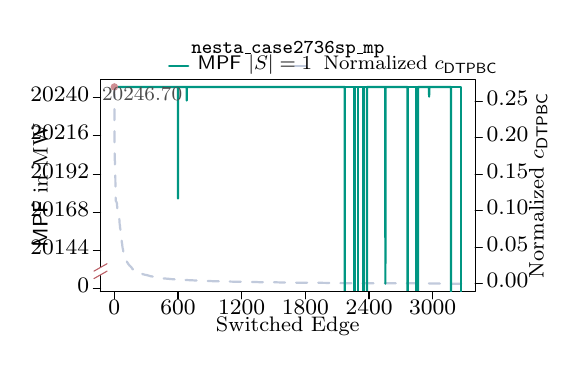
\begin{tikzpicture}[x=1pt,y=1pt]
\definecolor{fillColor}{RGB}{255,255,255}
\path[use as bounding box,fill=fillColor,fill opacity=0.00] (0,0) rectangle (440.85,271.01);
\begin{scope}
\path[clip] (  0.00,  0.00) rectangle (440.85,271.01);
\definecolor{drawColor}{RGB}{193,202,220}

\path[draw=drawColor,line width= 0.8pt,dash pattern=on 4pt off 4pt ,line join=round,line cap=round] ( 72.86,221.20) --
	( 72.95,181.18) --
	( 73.04,169.52) --
	( 73.13,160.41) --
	( 73.22,159.42) --
	( 73.31,159.20) --
	( 73.40,153.83) --
	( 73.49,152.09) --
	( 73.57,149.58) --
	( 73.66,147.44) --
	( 73.75,136.79) --
	( 73.84,129.53) --
	( 73.93,127.98) --
	( 74.02,125.66) --
	( 74.11,125.33) --
	( 74.20,125.13) --
	( 74.29,125.12) --
	( 74.38,125.11) --
	( 74.47,124.76) --
	( 74.56,124.70) --
	( 74.65,124.48) --
	( 74.73,124.28) --
	( 74.82,123.86) --
	( 74.91,123.70) --
	( 75.00,123.51) --
	( 75.09,121.40) --
	( 75.18,121.14) --
	( 75.27,119.53) --
	( 75.36,118.71) --
	( 75.45,118.27) --
	( 75.54,118.10) --
	( 75.63,117.67) --
	( 75.72,117.24) --
	( 75.80,116.60) --
	( 75.89,114.96) --
	( 75.98,114.55) --
	( 76.07,114.11) --
	( 76.16,113.96) --
	( 76.25,113.85) --
	( 76.34,113.22) --
	( 76.43,112.42) --
	( 76.52,112.36) --
	( 76.61,112.02) --
	( 76.70,111.16) --
	( 76.79,111.15) --
	( 76.88,111.00) --
	( 76.96,110.78) --
	( 77.05,109.98) --
	( 77.14,107.84) --
	( 77.23,107.46) --
	( 77.32,105.37) --
	( 77.41,105.17) --
	( 77.50,105.03) --
	( 77.59,103.29) --
	( 77.68,102.61) --
	( 77.77,102.55) --
	( 77.86,102.29) --
	( 77.95,100.56) --
	( 78.03, 98.52) --
	( 78.12, 98.32) --
	( 78.21, 98.23) --
	( 78.30, 97.13) --
	( 78.39, 95.68) --
	( 78.48, 95.62) --
	( 78.57, 94.12) --
	( 78.66, 93.86) --
	( 78.75, 92.59) --
	( 78.84, 92.31) --
	( 78.93, 92.11) --
	( 79.02, 91.55) --
	( 79.11, 90.52) --
	( 79.19, 90.34) --
	( 79.28, 90.10) --
	( 79.37, 89.17) --
	( 79.46, 88.89) --
	( 79.55, 87.59) --
	( 79.64, 86.87) --
	( 79.73, 86.69) --
	( 79.82, 85.66) --
	( 79.91, 85.22) --
	( 80.00, 85.19) --
	( 80.09, 85.12) --
	( 80.18, 84.65) --
	( 80.27, 83.21) --
	( 80.35, 83.10) --
	( 80.44, 82.82) --
	( 80.53, 82.44) --
	( 80.62, 81.84) --
	( 80.71, 81.09) --
	( 80.80, 80.50) --
	( 80.89, 80.39) --
	( 80.98, 80.24) --
	( 81.07, 80.18) --
	( 81.16, 80.15) --
	( 81.25, 79.88) --
	( 81.34, 79.81) --
	( 81.42, 79.72) --
	( 81.51, 79.54) --
	( 81.60, 79.51) --
	( 81.69, 78.64) --
	( 81.78, 78.32) --
	( 81.87, 78.10) --
	( 81.96, 77.95) --
	( 82.05, 77.86) --
	( 82.14, 77.67) --
	( 82.23, 77.51) --
	( 82.32, 77.18) --
	( 82.41, 77.10) --
	( 82.50, 76.62) --
	( 82.58, 76.18) --
	( 82.67, 76.18) --
	( 82.76, 76.07) --
	( 82.85, 75.89) --
	( 82.94, 75.62) --
	( 83.03, 75.53) --
	( 83.12, 75.39) --
	( 83.21, 75.35) --
	( 83.30, 74.97) --
	( 83.39, 74.49) --
	( 83.48, 74.03) --
	( 83.57, 73.91) --
	( 83.65, 73.76) --
	( 83.74, 73.70) --
	( 83.83, 73.66) --
	( 83.92, 73.47) --
	( 84.01, 73.38) --
	( 84.10, 73.22) --
	( 84.19, 73.20) --
	( 84.28, 72.86) --
	( 84.37, 72.84) --
	( 84.46, 72.83) --
	( 84.55, 72.44) --
	( 84.64, 72.36) --
	( 84.73, 72.32) --
	( 84.81, 71.85) --
	( 84.90, 71.85) --
	( 84.99, 71.81) --
	( 85.08, 71.78) --
	( 85.17, 71.71) --
	( 85.26, 71.66) --
	( 85.35, 71.29) --
	( 85.44, 71.28) --
	( 85.53, 71.17) --
	( 85.62, 71.16) --
	( 85.71, 70.99) --
	( 85.80, 70.85) --
	( 85.89, 70.83) --
	( 85.97, 70.80) --
	( 86.06, 70.75) --
	( 86.15, 70.54) --
	( 86.24, 70.53) --
	( 86.33, 70.45) --
	( 86.42, 70.32) --
	( 86.51, 70.29) --
	( 86.60, 70.24) --
	( 86.69, 70.04) --
	( 86.78, 69.87) --
	( 86.87, 69.84) --
	( 86.96, 69.72) --
	( 87.04, 69.71) --
	( 87.13, 69.59) --
	( 87.22, 69.53) --
	( 87.31, 69.52) --
	( 87.40, 69.35) --
	( 87.49, 68.99) --
	( 87.58, 68.99) --
	( 87.67, 68.95) --
	( 87.76, 68.92) --
	( 87.85, 68.53) --
	( 87.94, 68.49) --
	( 88.03, 68.36) --
	( 88.12, 68.09) --
	( 88.20, 68.04) --
	( 88.29, 68.02) --
	( 88.38, 68.01) --
	( 88.47, 67.99) --
	( 88.56, 67.98) --
	( 88.65, 67.85) --
	( 88.74, 67.82) --
	( 88.83, 67.57) --
	( 88.92, 67.56) --
	( 89.01, 67.37) --
	( 89.10, 67.33) --
	( 89.19, 67.26) --
	( 89.27, 67.14) --
	( 89.36, 67.06) --
	( 89.45, 67.06) --
	( 89.54, 67.00) --
	( 89.63, 66.89) --
	( 89.72, 66.87) --
	( 89.81, 66.86) --
	( 89.90, 66.83) --
	( 89.99, 66.73) --
	( 90.08, 66.70) --
	( 90.17, 66.63) --
	( 90.26, 66.60) --
	( 90.35, 66.59) --
	( 90.43, 66.51) --
	( 90.52, 66.32) --
	( 90.61, 66.31) --
	( 90.70, 66.31) --
	( 90.79, 66.15) --
	( 90.88, 66.14) --
	( 90.97, 66.06) --
	( 91.06, 66.06) --
	( 91.15, 66.05) --
	( 91.24, 66.04) --
	( 91.33, 66.01) --
	( 91.42, 65.98) --
	( 91.51, 65.86) --
	( 91.59, 65.64) --
	( 91.68, 65.58) --
	( 91.77, 65.55) --
	( 91.86, 65.46) --
	( 91.95, 65.43) --
	( 92.04, 65.41) --
	( 92.13, 65.39) --
	( 92.22, 65.35) --
	( 92.31, 65.29) --
	( 92.40, 65.16) --
	( 92.49, 65.02) --
	( 92.58, 64.99) --
	( 92.66, 64.90) --
	( 92.75, 64.85) --
	( 92.84, 64.82) --
	( 92.93, 64.79) --
	( 93.02, 64.77) --
	( 93.11, 64.69) --
	( 93.20, 64.68) --
	( 93.29, 64.68) --
	( 93.38, 64.65) --
	( 93.47, 64.61) --
	( 93.56, 64.57) --
	( 93.65, 64.56) --
	( 93.74, 64.54) --
	( 93.82, 64.53) --
	( 93.91, 64.52) --
	( 94.00, 64.48) --
	( 94.09, 64.48) --
	( 94.18, 64.48) --
	( 94.27, 64.46) --
	( 94.36, 64.45) --
	( 94.45, 64.44) --
	( 94.54, 64.43) --
	( 94.63, 64.41) --
	( 94.72, 64.39) --
	( 94.81, 64.39) --
	( 94.89, 64.38) --
	( 94.98, 64.38) --
	( 95.07, 64.32) --
	( 95.16, 64.28) --
	( 95.25, 64.21) --
	( 95.34, 64.19) --
	( 95.43, 64.16) --
	( 95.52, 64.16) --
	( 95.61, 64.15) --
	( 95.70, 64.14) --
	( 95.79, 64.14) --
	( 95.88, 64.11) --
	( 95.97, 64.05) --
	( 96.05, 64.04) --
	( 96.14, 64.03) --
	( 96.23, 64.02) --
	( 96.32, 64.00) --
	( 96.41, 63.97) --
	( 96.50, 63.95) --
	( 96.59, 63.92) --
	( 96.68, 63.86) --
	( 96.77, 63.80) --
	( 96.86, 63.79) --
	( 96.95, 63.79) --
	( 97.04, 63.78) --
	( 97.13, 63.77) --
	( 97.21, 63.75) --
	( 97.30, 63.72) --
	( 97.39, 63.71) --
	( 97.48, 63.68) --
	( 97.57, 63.66) --
	( 97.66, 63.64) --
	( 97.75, 63.64) --
	( 97.84, 63.59) --
	( 97.93, 63.55) --
	( 98.02, 63.53) --
	( 98.11, 63.48) --
	( 98.20, 63.44) --
	( 98.28, 63.43) --
	( 98.37, 63.42) --
	( 98.46, 63.39) --
	( 98.55, 63.37) --
	( 98.64, 63.33) --
	( 98.73, 63.30) --
	( 98.82, 63.30) --
	( 98.91, 63.29) --
	( 99.00, 63.28) --
	( 99.09, 63.26) --
	( 99.18, 63.25) --
	( 99.27, 63.23) --
	( 99.36, 63.23) --
	( 99.44, 63.20) --
	( 99.53, 63.20) --
	( 99.62, 63.19) --
	( 99.71, 63.19) --
	( 99.80, 63.18) --
	( 99.89, 63.17) --
	( 99.98, 63.15) --
	(100.07, 63.09) --
	(100.16, 63.04) --
	(100.25, 62.97) --
	(100.34, 62.95) --
	(100.43, 62.95) --
	(100.51, 62.94) --
	(100.60, 62.92) --
	(100.69, 62.92) --
	(100.78, 62.92) --
	(100.87, 62.88) --
	(100.96, 62.84) --
	(101.05, 62.78) --
	(101.14, 62.77) --
	(101.23, 62.77) --
	(101.32, 62.74) --
	(101.41, 62.73) --
	(101.50, 62.70) --
	(101.59, 62.69) --
	(101.67, 62.68) --
	(101.76, 62.60) --
	(101.85, 62.60) --
	(101.94, 62.59) --
	(102.03, 62.53) --
	(102.12, 62.52) --
	(102.21, 62.51) --
	(102.30, 62.46) --
	(102.39, 62.39) --
	(102.48, 62.39) --
	(102.57, 62.35) --
	(102.66, 62.34) --
	(102.74, 62.30) --
	(102.83, 62.27) --
	(102.92, 62.27) --
	(103.01, 62.26) --
	(103.10, 62.19) --
	(103.19, 62.18) --
	(103.28, 62.16) --
	(103.37, 62.11) --
	(103.46, 62.09) --
	(103.55, 62.08) --
	(103.64, 62.08) --
	(103.73, 62.08) --
	(103.82, 62.06) --
	(103.90, 62.05) --
	(103.99, 62.03) --
	(104.08, 62.02) --
	(104.17, 62.02) --
	(104.26, 61.98) --
	(104.35, 61.95) --
	(104.44, 61.94) --
	(104.53, 61.89) --
	(104.62, 61.87) --
	(104.71, 61.87) --
	(104.80, 61.87) --
	(104.89, 61.85) --
	(104.98, 61.83) --
	(105.06, 61.80) --
	(105.15, 61.79) --
	(105.24, 61.77) --
	(105.33, 61.74) --
	(105.42, 61.73) --
	(105.51, 61.72) --
	(105.60, 61.71) --
	(105.69, 61.71) --
	(105.78, 61.69) --
	(105.87, 61.69) --
	(105.96, 61.67) --
	(106.05, 61.64) --
	(106.13, 61.61) --
	(106.22, 61.61) --
	(106.31, 61.59) --
	(106.40, 61.59) --
	(106.49, 61.59) --
	(106.58, 61.58) --
	(106.67, 61.58) --
	(106.76, 61.57) --
	(106.85, 61.56) --
	(106.94, 61.53) --
	(107.03, 61.50) --
	(107.12, 61.47) --
	(107.21, 61.45) --
	(107.29, 61.44) --
	(107.38, 61.44) --
	(107.47, 61.42) --
	(107.56, 61.40) --
	(107.65, 61.37) --
	(107.74, 61.35) --
	(107.83, 61.34) --
	(107.92, 61.32) --
	(108.01, 61.30) --
	(108.10, 61.30) --
	(108.19, 61.26) --
	(108.28, 61.26) --
	(108.36, 61.23) --
	(108.45, 61.22) --
	(108.54, 61.22) --
	(108.63, 61.21) --
	(108.72, 61.20) --
	(108.81, 61.20) --
	(108.90, 61.19) --
	(108.99, 61.19) --
	(109.08, 61.18) --
	(109.17, 61.16) --
	(109.26, 61.15) --
	(109.35, 61.14) --
	(109.44, 61.14) --
	(109.52, 61.11) --
	(109.61, 61.09) --
	(109.70, 61.09) --
	(109.79, 61.08) --
	(109.88, 61.05) --
	(109.97, 61.02) --
	(110.06, 61.01) --
	(110.15, 60.96) --
	(110.24, 60.90) --
	(110.33, 60.90) --
	(110.42, 60.84) --
	(110.51, 60.83) --
	(110.60, 60.83) --
	(110.68, 60.82) --
	(110.77, 60.82) --
	(110.86, 60.79) --
	(110.95, 60.78) --
	(111.04, 60.78) --
	(111.13, 60.77) --
	(111.22, 60.76) --
	(111.31, 60.72) --
	(111.40, 60.72) --
	(111.49, 60.71) --
	(111.58, 60.71) --
	(111.67, 60.69) --
	(111.75, 60.68) --
	(111.84, 60.66) --
	(111.93, 60.64) --
	(112.02, 60.62) --
	(112.11, 60.61) --
	(112.20, 60.61) --
	(112.29, 60.61) --
	(112.38, 60.59) --
	(112.47, 60.59) --
	(112.56, 60.59) --
	(112.65, 60.57) --
	(112.74, 60.56) --
	(112.83, 60.55) --
	(112.91, 60.55) --
	(113.00, 60.50) --
	(113.09, 60.48) --
	(113.18, 60.47) --
	(113.27, 60.46) --
	(113.36, 60.46) --
	(113.45, 60.45) --
	(113.54, 60.43) --
	(113.63, 60.43) --
	(113.72, 60.42) --
	(113.81, 60.42) --
	(113.90, 60.38) --
	(113.98, 60.38) --
	(114.07, 60.37) --
	(114.16, 60.35) --
	(114.25, 60.32) --
	(114.34, 60.30) --
	(114.43, 60.30) --
	(114.52, 60.29) --
	(114.61, 60.29) --
	(114.70, 60.27) --
	(114.79, 60.27) --
	(114.88, 60.27) --
	(114.97, 60.27) --
	(115.06, 60.26) --
	(115.14, 60.25) --
	(115.23, 60.23) --
	(115.32, 60.23) --
	(115.41, 60.21) --
	(115.50, 60.18) --
	(115.59, 60.18) --
	(115.68, 60.17) --
	(115.77, 60.17) --
	(115.86, 60.17) --
	(115.95, 60.17) --
	(116.04, 60.17) --
	(116.13, 60.17) --
	(116.22, 60.15) --
	(116.30, 60.14) --
	(116.39, 60.13) --
	(116.48, 60.12) --
	(116.57, 60.11) --
	(116.66, 60.10) --
	(116.75, 60.09) --
	(116.84, 60.07) --
	(116.93, 60.06) --
	(117.02, 60.05) --
	(117.11, 60.05) --
	(117.20, 60.04) --
	(117.29, 60.04) --
	(117.37, 60.04) --
	(117.46, 60.03) --
	(117.55, 60.03) --
	(117.64, 60.03) --
	(117.73, 60.02) --
	(117.82, 60.01) --
	(117.91, 60.01) --
	(118.00, 59.99) --
	(118.09, 59.99) --
	(118.18, 59.99) --
	(118.27, 59.98) --
	(118.36, 59.98) --
	(118.45, 59.98) --
	(118.53, 59.97) --
	(118.62, 59.96) --
	(118.71, 59.92) --
	(118.80, 59.92) --
	(118.89, 59.91) --
	(118.98, 59.90) --
	(119.07, 59.88) --
	(119.16, 59.88) --
	(119.25, 59.88) --
	(119.34, 59.87) --
	(119.43, 59.87) --
	(119.52, 59.87) --
	(119.60, 59.86) --
	(119.69, 59.84) --
	(119.78, 59.84) --
	(119.87, 59.83) --
	(119.96, 59.79) --
	(120.05, 59.78) --
	(120.14, 59.78) --
	(120.23, 59.77) --
	(120.32, 59.76) --
	(120.41, 59.75) --
	(120.50, 59.75) --
	(120.59, 59.72) --
	(120.68, 59.71) --
	(120.76, 59.71) --
	(120.85, 59.71) --
	(120.94, 59.70) --
	(121.03, 59.70) --
	(121.12, 59.69) --
	(121.21, 59.69) --
	(121.30, 59.67) --
	(121.39, 59.67) --
	(121.48, 59.67) --
	(121.57, 59.66) --
	(121.66, 59.65) --
	(121.75, 59.64) --
	(121.84, 59.64) --
	(121.92, 59.63) --
	(122.01, 59.63) --
	(122.10, 59.63) --
	(122.19, 59.61) --
	(122.28, 59.60) --
	(122.37, 59.60) --
	(122.46, 59.60) --
	(122.55, 59.60) --
	(122.64, 59.56) --
	(122.73, 59.56) --
	(122.82, 59.55) --
	(122.91, 59.55) --
	(122.99, 59.55) --
	(123.08, 59.54) --
	(123.17, 59.53) --
	(123.26, 59.53) --
	(123.35, 59.51) --
	(123.44, 59.51) --
	(123.53, 59.51) --
	(123.62, 59.49) --
	(123.71, 59.48) --
	(123.80, 59.48) --
	(123.89, 59.47) --
	(123.98, 59.47) --
	(124.07, 59.47) --
	(124.15, 59.45) --
	(124.24, 59.44) --
	(124.33, 59.44) --
	(124.42, 59.44) --
	(124.51, 59.44) --
	(124.60, 59.43) --
	(124.69, 59.43) --
	(124.78, 59.42) --
	(124.87, 59.42) --
	(124.96, 59.42) --
	(125.05, 59.42) --
	(125.14, 59.41) --
	(125.22, 59.40) --
	(125.31, 59.39) --
	(125.40, 59.38) --
	(125.49, 59.38) --
	(125.58, 59.38) --
	(125.67, 59.36) --
	(125.76, 59.36) --
	(125.85, 59.35) --
	(125.94, 59.35) --
	(126.03, 59.34) --
	(126.12, 59.33) --
	(126.21, 59.33) --
	(126.30, 59.32) --
	(126.38, 59.32) --
	(126.47, 59.30) --
	(126.56, 59.30) --
	(126.65, 59.30) --
	(126.74, 59.30) --
	(126.83, 59.28) --
	(126.92, 59.28) --
	(127.01, 59.28) --
	(127.10, 59.27) --
	(127.19, 59.27) --
	(127.28, 59.26) --
	(127.37, 59.26) --
	(127.46, 59.25) --
	(127.54, 59.25) --
	(127.63, 59.25) --
	(127.72, 59.25) --
	(127.81, 59.24) --
	(127.90, 59.23) --
	(127.99, 59.23) --
	(128.08, 59.22) --
	(128.17, 59.22) --
	(128.26, 59.21) --
	(128.35, 59.21) --
	(128.44, 59.21) --
	(128.53, 59.21) --
	(128.61, 59.20) --
	(128.70, 59.19) --
	(128.79, 59.19) --
	(128.88, 59.19) --
	(128.97, 59.18) --
	(129.06, 59.18) --
	(129.15, 59.17) --
	(129.24, 59.17) --
	(129.33, 59.17) --
	(129.42, 59.15) --
	(129.51, 59.15) --
	(129.60, 59.15) --
	(129.69, 59.14) --
	(129.77, 59.13) --
	(129.86, 59.12) --
	(129.95, 59.12) --
	(130.04, 59.12) --
	(130.13, 59.12) --
	(130.22, 59.11) --
	(130.31, 59.10) --
	(130.40, 59.10) --
	(130.49, 59.09) --
	(130.58, 59.09) --
	(130.67, 59.08) --
	(130.76, 59.08) --
	(130.84, 59.07) --
	(130.93, 59.07) --
	(131.02, 59.06) --
	(131.11, 59.06) --
	(131.20, 59.05) --
	(131.29, 59.04) --
	(131.38, 59.03) --
	(131.47, 59.03) --
	(131.56, 59.02) --
	(131.65, 59.01) --
	(131.74, 59.01) --
	(131.83, 59.01) --
	(131.92, 59.01) --
	(132.00, 59.00) --
	(132.09, 59.00) --
	(132.18, 59.00) --
	(132.27, 59.00) --
	(132.36, 58.98) --
	(132.45, 58.98) --
	(132.54, 58.97) --
	(132.63, 58.97) --
	(132.72, 58.96) --
	(132.81, 58.96) --
	(132.90, 58.96) --
	(132.99, 58.94) --
	(133.08, 58.93) --
	(133.16, 58.92) --
	(133.25, 58.92) --
	(133.34, 58.91) --
	(133.43, 58.90) --
	(133.52, 58.90) --
	(133.61, 58.90) --
	(133.70, 58.90) --
	(133.79, 58.90) --
	(133.88, 58.89) --
	(133.97, 58.89) --
	(134.06, 58.88) --
	(134.15, 58.88) --
	(134.23, 58.88) --
	(134.32, 58.88) --
	(134.41, 58.88) --
	(134.50, 58.88) --
	(134.59, 58.87) --
	(134.68, 58.87) --
	(134.77, 58.87) --
	(134.86, 58.87) --
	(134.95, 58.87) --
	(135.04, 58.86) --
	(135.13, 58.86) --
	(135.22, 58.86) --
	(135.31, 58.86) --
	(135.39, 58.85) --
	(135.48, 58.85) --
	(135.57, 58.84) --
	(135.66, 58.84) --
	(135.75, 58.84) --
	(135.84, 58.83) --
	(135.93, 58.82) --
	(136.02, 58.81) --
	(136.11, 58.81) --
	(136.20, 58.81) --
	(136.29, 58.80) --
	(136.38, 58.79) --
	(136.46, 58.78) --
	(136.55, 58.78) --
	(136.64, 58.77) --
	(136.73, 58.77) --
	(136.82, 58.77) --
	(136.91, 58.77) --
	(137.00, 58.77) --
	(137.09, 58.77) --
	(137.18, 58.76) --
	(137.27, 58.76) --
	(137.36, 58.76) --
	(137.45, 58.76) --
	(137.54, 58.75) --
	(137.62, 58.75) --
	(137.71, 58.73) --
	(137.80, 58.73) --
	(137.89, 58.73) --
	(137.98, 58.70) --
	(138.07, 58.70) --
	(138.16, 58.70) --
	(138.25, 58.70) --
	(138.34, 58.69) --
	(138.43, 58.69) --
	(138.52, 58.69) --
	(138.61, 58.69) --
	(138.69, 58.67) --
	(138.78, 58.67) --
	(138.87, 58.67) --
	(138.96, 58.66) --
	(139.05, 58.65) --
	(139.14, 58.65) --
	(139.23, 58.65) --
	(139.32, 58.65) --
	(139.41, 58.65) --
	(139.50, 58.64) --
	(139.59, 58.64) --
	(139.68, 58.64) --
	(139.77, 58.63) --
	(139.85, 58.63) --
	(139.94, 58.63) --
	(140.03, 58.62) --
	(140.12, 58.62) --
	(140.21, 58.61) --
	(140.30, 58.60) --
	(140.39, 58.60) --
	(140.48, 58.60) --
	(140.57, 58.58) --
	(140.66, 58.58) --
	(140.75, 58.57) --
	(140.84, 58.57) --
	(140.93, 58.56) --
	(141.01, 58.55) --
	(141.10, 58.55) --
	(141.19, 58.55) --
	(141.28, 58.53) --
	(141.37, 58.53) --
	(141.46, 58.53) --
	(141.55, 58.53) --
	(141.64, 58.53) --
	(141.73, 58.53) --
	(141.82, 58.52) --
	(141.91, 58.51) --
	(142.00, 58.50) --
	(142.08, 58.50) --
	(142.17, 58.50) --
	(142.26, 58.49) --
	(142.35, 58.48) --
	(142.44, 58.48) --
	(142.53, 58.48) --
	(142.62, 58.47) --
	(142.71, 58.47) --
	(142.80, 58.46) --
	(142.89, 58.46) --
	(142.98, 58.45) --
	(143.07, 58.44) --
	(143.16, 58.44) --
	(143.24, 58.44) --
	(143.33, 58.44) --
	(143.42, 58.44) --
	(143.51, 58.44) --
	(143.60, 58.43) --
	(143.69, 58.43) --
	(143.78, 58.42) --
	(143.87, 58.42) --
	(143.96, 58.42) --
	(144.05, 58.42) --
	(144.14, 58.42) --
	(144.23, 58.41) --
	(144.31, 58.41) --
	(144.40, 58.41) --
	(144.49, 58.40) --
	(144.58, 58.39) --
	(144.67, 58.39) --
	(144.76, 58.39) --
	(144.85, 58.38) --
	(144.94, 58.38) --
	(145.03, 58.38) --
	(145.12, 58.37) --
	(145.21, 58.37) --
	(145.30, 58.37) --
	(145.39, 58.37) --
	(145.47, 58.36) --
	(145.56, 58.36) --
	(145.65, 58.35) --
	(145.74, 58.35) --
	(145.83, 58.35) --
	(145.92, 58.34) --
	(146.01, 58.34) --
	(146.10, 58.34) --
	(146.19, 58.33) --
	(146.28, 58.33) --
	(146.37, 58.32) --
	(146.46, 58.32) --
	(146.55, 58.32) --
	(146.63, 58.32) --
	(146.72, 58.31) --
	(146.81, 58.31) --
	(146.90, 58.30) --
	(146.99, 58.29) --
	(147.08, 58.29) --
	(147.17, 58.28) --
	(147.26, 58.28) --
	(147.35, 58.28) --
	(147.44, 58.28) --
	(147.53, 58.27) --
	(147.62, 58.27) --
	(147.70, 58.27) --
	(147.79, 58.27) --
	(147.88, 58.27) --
	(147.97, 58.26) --
	(148.06, 58.25) --
	(148.15, 58.25) --
	(148.24, 58.25) --
	(148.33, 58.24) --
	(148.42, 58.24) --
	(148.51, 58.24) --
	(148.60, 58.23) --
	(148.69, 58.22) --
	(148.78, 58.22) --
	(148.86, 58.22) --
	(148.95, 58.22) --
	(149.04, 58.22) --
	(149.13, 58.21) --
	(149.22, 58.20) --
	(149.31, 58.20) --
	(149.40, 58.20) --
	(149.49, 58.20) --
	(149.58, 58.20) --
	(149.67, 58.19) --
	(149.76, 58.19) --
	(149.85, 58.19) --
	(149.93, 58.19) --
	(150.02, 58.19) --
	(150.11, 58.18) --
	(150.20, 58.18) --
	(150.29, 58.18) --
	(150.38, 58.17) --
	(150.47, 58.17) --
	(150.56, 58.16) --
	(150.65, 58.16) --
	(150.74, 58.16) --
	(150.83, 58.16) --
	(150.92, 58.16) --
	(151.01, 58.15) --
	(151.09, 58.15) --
	(151.18, 58.15) --
	(151.27, 58.15) --
	(151.36, 58.15) --
	(151.45, 58.15) --
	(151.54, 58.14) --
	(151.63, 58.14) --
	(151.72, 58.14) --
	(151.81, 58.14) --
	(151.90, 58.14) --
	(151.99, 58.13) --
	(152.08, 58.13) --
	(152.17, 58.13) --
	(152.25, 58.13) --
	(152.34, 58.13) --
	(152.43, 58.13) --
	(152.52, 58.12) --
	(152.61, 58.12) --
	(152.70, 58.11) --
	(152.79, 58.11) --
	(152.88, 58.10) --
	(152.97, 58.09) --
	(153.06, 58.08) --
	(153.15, 58.08) --
	(153.24, 58.08) --
	(153.32, 58.08) --
	(153.41, 58.08) --
	(153.50, 58.07) --
	(153.59, 58.06) --
	(153.68, 58.06) --
	(153.77, 58.05) --
	(153.86, 58.04) --
	(153.95, 58.04) --
	(154.04, 58.04) --
	(154.13, 58.04) --
	(154.22, 58.04) --
	(154.31, 58.02) --
	(154.40, 58.02) --
	(154.48, 58.02) --
	(154.57, 58.02) --
	(154.66, 58.02) --
	(154.75, 58.01) --
	(154.84, 58.01) --
	(154.93, 58.01) --
	(155.02, 58.00) --
	(155.11, 58.00) --
	(155.20, 58.00) --
	(155.29, 58.00) --
	(155.38, 58.00) --
	(155.47, 58.00) --
	(155.55, 58.00) --
	(155.64, 58.00) --
	(155.73, 58.00) --
	(155.82, 58.00) --
	(155.91, 57.99) --
	(156.00, 57.99) --
	(156.09, 57.99) --
	(156.18, 57.99) --
	(156.27, 57.99) --
	(156.36, 57.98) --
	(156.45, 57.98) --
	(156.54, 57.98) --
	(156.63, 57.98) --
	(156.71, 57.97) --
	(156.80, 57.97) --
	(156.89, 57.97) --
	(156.98, 57.97) --
	(157.07, 57.97) --
	(157.16, 57.97) --
	(157.25, 57.96) --
	(157.34, 57.96) --
	(157.43, 57.96) --
	(157.52, 57.95) --
	(157.61, 57.95) --
	(157.70, 57.95) --
	(157.79, 57.95) --
	(157.87, 57.94) --
	(157.96, 57.94) --
	(158.05, 57.94) --
	(158.14, 57.94) --
	(158.23, 57.94) --
	(158.32, 57.94) --
	(158.41, 57.94) --
	(158.50, 57.94) --
	(158.59, 57.94) --
	(158.68, 57.92) --
	(158.77, 57.92) --
	(158.86, 57.92) --
	(158.94, 57.92) --
	(159.03, 57.91) --
	(159.12, 57.91) --
	(159.21, 57.91) --
	(159.30, 57.91) --
	(159.39, 57.91) --
	(159.48, 57.90) --
	(159.57, 57.90) --
	(159.66, 57.90) --
	(159.75, 57.90) --
	(159.84, 57.90) --
	(159.93, 57.89) --
	(160.02, 57.89) --
	(160.10, 57.89) --
	(160.19, 57.89) --
	(160.28, 57.89) --
	(160.37, 57.88) --
	(160.46, 57.88) --
	(160.55, 57.88) --
	(160.64, 57.87) --
	(160.73, 57.87) --
	(160.82, 57.87) --
	(160.91, 57.87) --
	(161.00, 57.87) --
	(161.09, 57.86) --
	(161.17, 57.86) --
	(161.26, 57.86) --
	(161.35, 57.84) --
	(161.44, 57.84) --
	(161.53, 57.84) --
	(161.62, 57.83) --
	(161.71, 57.83) --
	(161.80, 57.83) --
	(161.89, 57.83) --
	(161.98, 57.83) --
	(162.07, 57.82) --
	(162.16, 57.82) --
	(162.25, 57.82) --
	(162.33, 57.82) --
	(162.42, 57.81) --
	(162.51, 57.81) --
	(162.60, 57.81) --
	(162.69, 57.80) --
	(162.78, 57.79) --
	(162.87, 57.79) --
	(162.96, 57.78) --
	(163.05, 57.78) --
	(163.14, 57.78) --
	(163.23, 57.78) --
	(163.32, 57.78) --
	(163.41, 57.78) --
	(163.49, 57.78) --
	(163.58, 57.78) --
	(163.67, 57.77) --
	(163.76, 57.77) --
	(163.85, 57.77) --
	(163.94, 57.76) --
	(164.03, 57.76) --
	(164.12, 57.76) --
	(164.21, 57.76) --
	(164.30, 57.76) --
	(164.39, 57.76) --
	(164.48, 57.76) --
	(164.56, 57.75) --
	(164.65, 57.75) --
	(164.74, 57.75) --
	(164.83, 57.74) --
	(164.92, 57.74) --
	(165.01, 57.74) --
	(165.10, 57.74) --
	(165.19, 57.74) --
	(165.28, 57.74) --
	(165.37, 57.73) --
	(165.46, 57.73) --
	(165.55, 57.73) --
	(165.64, 57.72) --
	(165.72, 57.72) --
	(165.81, 57.72) --
	(165.90, 57.72) --
	(165.99, 57.71) --
	(166.08, 57.71) --
	(166.17, 57.71) --
	(166.26, 57.71) --
	(166.35, 57.70) --
	(166.44, 57.70) --
	(166.53, 57.70) --
	(166.62, 57.70) --
	(166.71, 57.70) --
	(166.79, 57.70) --
	(166.88, 57.69) --
	(166.97, 57.69) --
	(167.06, 57.69) --
	(167.15, 57.69) --
	(167.24, 57.68) --
	(167.33, 57.68) --
	(167.42, 57.68) --
	(167.51, 57.68) --
	(167.60, 57.68) --
	(167.69, 57.68) --
	(167.78, 57.67) --
	(167.87, 57.67) --
	(167.95, 57.67) --
	(168.04, 57.67) --
	(168.13, 57.67) --
	(168.22, 57.66) --
	(168.31, 57.66) --
	(168.40, 57.65) --
	(168.49, 57.65) --
	(168.58, 57.65) --
	(168.67, 57.65) --
	(168.76, 57.65) --
	(168.85, 57.65) --
	(168.94, 57.65) --
	(169.02, 57.65) --
	(169.11, 57.64) --
	(169.20, 57.64) --
	(169.29, 57.64) --
	(169.38, 57.64) --
	(169.47, 57.64) --
	(169.56, 57.64) --
	(169.65, 57.63) --
	(169.74, 57.63) --
	(169.83, 57.63) --
	(169.92, 57.63) --
	(170.01, 57.63) --
	(170.10, 57.63) --
	(170.18, 57.62) --
	(170.27, 57.62) --
	(170.36, 57.62) --
	(170.45, 57.62) --
	(170.54, 57.62) --
	(170.63, 57.61) --
	(170.72, 57.61) --
	(170.81, 57.61) --
	(170.90, 57.61) --
	(170.99, 57.61) --
	(171.08, 57.61) --
	(171.17, 57.60) --
	(171.26, 57.60) --
	(171.34, 57.60) --
	(171.43, 57.60) --
	(171.52, 57.60) --
	(171.61, 57.60) --
	(171.70, 57.59) --
	(171.79, 57.59) --
	(171.88, 57.59) --
	(171.97, 57.59) --
	(172.06, 57.58) --
	(172.15, 57.58) --
	(172.24, 57.58) --
	(172.33, 57.58) --
	(172.41, 57.58) --
	(172.50, 57.57) --
	(172.59, 57.57) --
	(172.68, 57.57) --
	(172.77, 57.57) --
	(172.86, 57.57) --
	(172.95, 57.57) --
	(173.04, 57.57) --
	(173.13, 57.57) --
	(173.22, 57.57) --
	(173.31, 57.56) --
	(173.40, 57.56) --
	(173.49, 57.56) --
	(173.57, 57.56) --
	(173.66, 57.56) --
	(173.75, 57.56) --
	(173.84, 57.56) --
	(173.93, 57.56) --
	(174.02, 57.56) --
	(174.11, 57.56) --
	(174.20, 57.56) --
	(174.29, 57.56) --
	(174.38, 57.56) --
	(174.47, 57.55) --
	(174.56, 57.55) --
	(174.64, 57.55) --
	(174.73, 57.55) --
	(174.82, 57.54) --
	(174.91, 57.54) --
	(175.00, 57.54) --
	(175.09, 57.54) --
	(175.18, 57.54) --
	(175.27, 57.53) --
	(175.36, 57.53) --
	(175.45, 57.53) --
	(175.54, 57.53) --
	(175.63, 57.53) --
	(175.72, 57.52) --
	(175.80, 57.52) --
	(175.89, 57.52) --
	(175.98, 57.52) --
	(176.07, 57.52) --
	(176.16, 57.52) --
	(176.25, 57.52) --
	(176.34, 57.52) --
	(176.43, 57.51) --
	(176.52, 57.51) --
	(176.61, 57.51) --
	(176.70, 57.51) --
	(176.79, 57.50) --
	(176.88, 57.50) --
	(176.96, 57.50) --
	(177.05, 57.50) --
	(177.14, 57.49) --
	(177.23, 57.49) --
	(177.32, 57.49) --
	(177.41, 57.49) --
	(177.50, 57.49) --
	(177.59, 57.49) --
	(177.68, 57.49) --
	(177.77, 57.49) --
	(177.86, 57.49) --
	(177.95, 57.49) --
	(178.03, 57.48) --
	(178.12, 57.48) --
	(178.21, 57.48) --
	(178.30, 57.48) --
	(178.39, 57.47) --
	(178.48, 57.47) --
	(178.57, 57.47) --
	(178.66, 57.47) --
	(178.75, 57.47) --
	(178.84, 57.47) --
	(178.93, 57.47) --
	(179.02, 57.47) --
	(179.11, 57.47) --
	(179.19, 57.46) --
	(179.28, 57.46) --
	(179.37, 57.46) --
	(179.46, 57.46) --
	(179.55, 57.46) --
	(179.64, 57.46) --
	(179.73, 57.46) --
	(179.82, 57.46) --
	(179.91, 57.46) --
	(180.00, 57.46) --
	(180.09, 57.46) --
	(180.18, 57.46) --
	(180.26, 57.46) --
	(180.35, 57.45) --
	(180.44, 57.45) --
	(180.53, 57.45) --
	(180.62, 57.45) --
	(180.71, 57.45) --
	(180.80, 57.44) --
	(180.89, 57.44) --
	(180.98, 57.44) --
	(181.07, 57.44) --
	(181.16, 57.44) --
	(181.25, 57.44) --
	(181.34, 57.43) --
	(181.42, 57.43) --
	(181.51, 57.43) --
	(181.60, 57.43) --
	(181.69, 57.43) --
	(181.78, 57.43) --
	(181.87, 57.43) --
	(181.96, 57.42) --
	(182.05, 57.42) --
	(182.14, 57.42) --
	(182.23, 57.42) --
	(182.32, 57.41) --
	(182.41, 57.41) --
	(182.50, 57.41) --
	(182.58, 57.41) --
	(182.67, 57.40) --
	(182.76, 57.40) --
	(182.85, 57.40) --
	(182.94, 57.40) --
	(183.03, 57.40) --
	(183.12, 57.40) --
	(183.21, 57.39) --
	(183.30, 57.39) --
	(183.39, 57.39) --
	(183.48, 57.39) --
	(183.57, 57.39) --
	(183.65, 57.39) --
	(183.74, 57.39) --
	(183.83, 57.38) --
	(183.92, 57.38) --
	(184.01, 57.37) --
	(184.10, 57.37) --
	(184.19, 57.37) --
	(184.28, 57.37) --
	(184.37, 57.36) --
	(184.46, 57.36) --
	(184.55, 57.36) --
	(184.64, 57.36) --
	(184.73, 57.36) --
	(184.81, 57.36) --
	(184.90, 57.35) --
	(184.99, 57.35) --
	(185.08, 57.35) --
	(185.17, 57.35) --
	(185.26, 57.34) --
	(185.35, 57.34) --
	(185.44, 57.33) --
	(185.53, 57.33) --
	(185.62, 57.33) --
	(185.71, 57.33) --
	(185.80, 57.33) --
	(185.88, 57.33) --
	(185.97, 57.33) --
	(186.06, 57.33) --
	(186.15, 57.33) --
	(186.24, 57.32) --
	(186.33, 57.32) --
	(186.42, 57.32) --
	(186.51, 57.32) --
	(186.60, 57.31) --
	(186.69, 57.31) --
	(186.78, 57.30) --
	(186.87, 57.30) --
	(186.96, 57.30) --
	(187.04, 57.30) --
	(187.13, 57.29) --
	(187.22, 57.29) --
	(187.31, 57.29) --
	(187.40, 57.29) --
	(187.49, 57.29) --
	(187.58, 57.29) --
	(187.67, 57.29) --
	(187.76, 57.29) --
	(187.85, 57.28) --
	(187.94, 57.28) --
	(188.03, 57.28) --
	(188.12, 57.28) --
	(188.20, 57.28) --
	(188.29, 57.28) --
	(188.38, 57.28) --
	(188.47, 57.28) --
	(188.56, 57.28) --
	(188.65, 57.28) --
	(188.74, 57.27) --
	(188.83, 57.27) --
	(188.92, 57.27) --
	(189.01, 57.27) --
	(189.10, 57.27) --
	(189.19, 57.27) --
	(189.27, 57.26) --
	(189.36, 57.26) --
	(189.45, 57.26) --
	(189.54, 57.26) --
	(189.63, 57.26) --
	(189.72, 57.25) --
	(189.81, 57.25) --
	(189.90, 57.25) --
	(189.99, 57.25) --
	(190.08, 57.25) --
	(190.17, 57.24) --
	(190.26, 57.24) --
	(190.35, 57.24) --
	(190.43, 57.24) --
	(190.52, 57.24) --
	(190.61, 57.24) --
	(190.70, 57.23) --
	(190.79, 57.23) --
	(190.88, 57.23) --
	(190.97, 57.23) --
	(191.06, 57.23) --
	(191.15, 57.22) --
	(191.24, 57.22) --
	(191.33, 57.22) --
	(191.42, 57.22) --
	(191.50, 57.22) --
	(191.59, 57.22) --
	(191.68, 57.22) --
	(191.77, 57.22) --
	(191.86, 57.21) --
	(191.95, 57.21) --
	(192.04, 57.21) --
	(192.13, 57.21) --
	(192.22, 57.21) --
	(192.31, 57.21) --
	(192.40, 57.21) --
	(192.49, 57.21) --
	(192.58, 57.20) --
	(192.66, 57.20) --
	(192.75, 57.20) --
	(192.84, 57.20) --
	(192.93, 57.20) --
	(193.02, 57.20) --
	(193.11, 57.19) --
	(193.20, 57.19) --
	(193.29, 57.19) --
	(193.38, 57.19) --
	(193.47, 57.19) --
	(193.56, 57.19) --
	(193.65, 57.18) --
	(193.74, 57.18) --
	(193.82, 57.18) --
	(193.91, 57.17) --
	(194.00, 57.17) --
	(194.09, 57.17) --
	(194.18, 57.16) --
	(194.27, 57.16) --
	(194.36, 57.16) --
	(194.45, 57.16) --
	(194.54, 57.16) --
	(194.63, 57.16) --
	(194.72, 57.16) --
	(194.81, 57.15) --
	(194.89, 57.15) --
	(194.98, 57.15) --
	(195.07, 57.15) --
	(195.16, 57.14) --
	(195.25, 57.14) --
	(195.34, 57.14) --
	(195.43, 57.14) --
	(195.52, 57.14) --
	(195.61, 57.14) --
	(195.70, 57.14) --
	(195.79, 57.14) --
	(195.88, 57.13) --
	(195.97, 57.13) --
	(196.05, 57.13) --
	(196.14, 57.13) --
	(196.23, 57.13) --
	(196.32, 57.13) --
	(196.41, 57.13) --
	(196.50, 57.13) --
	(196.59, 57.13) --
	(196.68, 57.13) --
	(196.77, 57.13) --
	(196.86, 57.13) --
	(196.95, 57.13) --
	(197.04, 57.13) --
	(197.12, 57.13) --
	(197.21, 57.13) --
	(197.30, 57.13) --
	(197.39, 57.13) --
	(197.48, 57.13) --
	(197.57, 57.12) --
	(197.66, 57.12) --
	(197.75, 57.12) --
	(197.84, 57.12) --
	(197.93, 57.12) --
	(198.02, 57.12) --
	(198.11, 57.12) --
	(198.20, 57.12) --
	(198.28, 57.12) --
	(198.37, 57.12) --
	(198.46, 57.12) --
	(198.55, 57.12) --
	(198.64, 57.12) --
	(198.73, 57.12) --
	(198.82, 57.12) --
	(198.91, 57.12) --
	(199.00, 57.12) --
	(199.09, 57.12) --
	(199.18, 57.12) --
	(199.27, 57.12) --
	(199.36, 57.12) --
	(199.44, 57.12) --
	(199.53, 57.12) --
	(199.62, 57.11) --
	(199.71, 57.11) --
	(199.80, 57.11) --
	(199.89, 57.11) --
	(199.98, 57.11) --
	(200.07, 57.11) --
	(200.16, 57.10) --
	(200.25, 57.10) --
	(200.34, 57.10) --
	(200.43, 57.10) --
	(200.51, 57.10) --
	(200.60, 57.10) --
	(200.69, 57.10) --
	(200.78, 57.10) --
	(200.87, 57.10) --
	(200.96, 57.10) --
	(201.05, 57.10) --
	(201.14, 57.10) --
	(201.23, 57.09) --
	(201.32, 57.09) --
	(201.41, 57.09) --
	(201.50, 57.09) --
	(201.59, 57.09) --
	(201.67, 57.09) --
	(201.76, 57.09) --
	(201.85, 57.09) --
	(201.94, 57.09) --
	(202.03, 57.09) --
	(202.12, 57.09) --
	(202.21, 57.09) --
	(202.30, 57.09) --
	(202.39, 57.08) --
	(202.48, 57.08) --
	(202.57, 57.08) --
	(202.66, 57.08) --
	(202.74, 57.08) --
	(202.83, 57.07) --
	(202.92, 57.07) --
	(203.01, 57.07) --
	(203.10, 57.07) --
	(203.19, 57.07) --
	(203.28, 57.07) --
	(203.37, 57.07) --
	(203.46, 57.06) --
	(203.55, 57.06) --
	(203.64, 57.06) --
	(203.73, 57.06) --
	(203.82, 57.06) --
	(203.90, 57.06) --
	(203.99, 57.06) --
	(204.08, 57.06) --
	(204.17, 57.06) --
	(204.26, 57.06) --
	(204.35, 57.06) --
	(204.44, 57.05) --
	(204.53, 57.05) --
	(204.62, 57.05) --
	(204.71, 57.05) --
	(204.80, 57.05) --
	(204.89, 57.05) --
	(204.97, 57.05) --
	(205.06, 57.04) --
	(205.15, 57.04) --
	(205.24, 57.04) --
	(205.33, 57.04) --
	(205.42, 57.04) --
	(205.51, 57.04) --
	(205.60, 57.04) --
	(205.69, 57.04) --
	(205.78, 57.04) --
	(205.87, 57.04) --
	(205.96, 57.04) --
	(206.05, 57.03) --
	(206.13, 57.03) --
	(206.22, 57.03) --
	(206.31, 57.03) --
	(206.40, 57.02) --
	(206.49, 57.02) --
	(206.58, 57.02) --
	(206.67, 57.02) --
	(206.76, 57.02) --
	(206.85, 57.02) --
	(206.94, 57.02) --
	(207.03, 57.02) --
	(207.12, 57.02) --
	(207.21, 57.02) --
	(207.29, 57.02) --
	(207.38, 57.02) --
	(207.47, 57.02) --
	(207.56, 57.01) --
	(207.65, 57.01) --
	(207.74, 57.01) --
	(207.83, 57.01) --
	(207.92, 57.01) --
	(208.01, 57.00) --
	(208.10, 57.00) --
	(208.19, 57.00) --
	(208.28, 57.00) --
	(208.36, 57.00) --
	(208.45, 57.00) --
	(208.54, 57.00) --
	(208.63, 57.00) --
	(208.72, 57.00) --
	(208.81, 57.00) --
	(208.90, 57.00) --
	(208.99, 57.00) --
	(209.08, 57.00) --
	(209.17, 56.99) --
	(209.26, 56.99) --
	(209.35, 56.99) --
	(209.44, 56.99) --
	(209.52, 56.99) --
	(209.61, 56.99) --
	(209.70, 56.98) --
	(209.79, 56.98) --
	(209.88, 56.98) --
	(209.97, 56.98) --
	(210.06, 56.98) --
	(210.15, 56.98) --
	(210.24, 56.98) --
	(210.33, 56.97) --
	(210.42, 56.97) --
	(210.51, 56.97) --
	(210.59, 56.97) --
	(210.68, 56.97) --
	(210.77, 56.97) --
	(210.86, 56.97) --
	(210.95, 56.97) --
	(211.04, 56.97) --
	(211.13, 56.96) --
	(211.22, 56.96) --
	(211.31, 56.95) --
	(211.40, 56.95) --
	(211.49, 56.95) --
	(211.58, 56.95) --
	(211.67, 56.95) --
	(211.75, 56.95) --
	(211.84, 56.95) --
	(211.93, 56.95) --
	(212.02, 56.95) --
	(212.11, 56.95) --
	(212.20, 56.94) --
	(212.29, 56.94) --
	(212.38, 56.94) --
	(212.47, 56.94) --
	(212.56, 56.94) --
	(212.65, 56.94) --
	(212.74, 56.93) --
	(212.83, 56.93) --
	(212.91, 56.93) --
	(213.00, 56.93) --
	(213.09, 56.92) --
	(213.18, 56.92) --
	(213.27, 56.92) --
	(213.36, 56.92) --
	(213.45, 56.92) --
	(213.54, 56.92) --
	(213.63, 56.92) --
	(213.72, 56.92) --
	(213.81, 56.91) --
	(213.90, 56.91) --
	(213.98, 56.91) --
	(214.07, 56.91) --
	(214.16, 56.91) --
	(214.25, 56.91) --
	(214.34, 56.91) --
	(214.43, 56.91) --
	(214.52, 56.90) --
	(214.61, 56.90) --
	(214.70, 56.90) --
	(214.79, 56.90) --
	(214.88, 56.90) --
	(214.97, 56.90) --
	(215.06, 56.90) --
	(215.14, 56.90) --
	(215.23, 56.89) --
	(215.32, 56.89) --
	(215.41, 56.89) --
	(215.50, 56.89) --
	(215.59, 56.89) --
	(215.68, 56.89) --
	(215.77, 56.89) --
	(215.86, 56.89) --
	(215.95, 56.88) --
	(216.04, 56.87) --
	(216.13, 56.87) --
	(216.21, 56.87) --
	(216.30, 56.87) --
	(216.39, 56.87) --
	(216.48, 56.87) --
	(216.57, 56.86) --
	(216.66, 56.86) --
	(216.75, 56.86) --
	(216.84, 56.86) --
	(216.93, 56.86) --
	(217.02, 56.85) --
	(217.11, 56.85) --
	(217.20, 56.85) --
	(217.29, 56.85) --
	(217.37, 56.85) --
	(217.46, 56.85) --
	(217.55, 56.85) --
	(217.64, 56.84) --
	(217.73, 56.84) --
	(217.82, 56.84) --
	(217.91, 56.84) --
	(218.00, 56.84) --
	(218.09, 56.83) --
	(218.18, 56.83) --
	(218.27, 56.83) --
	(218.36, 56.83) --
	(218.45, 56.82) --
	(218.53, 56.82) --
	(218.62, 56.82) --
	(218.71, 56.82) --
	(218.80, 56.82) --
	(218.89, 56.82) --
	(218.98, 56.82) --
	(219.07, 56.81) --
	(219.16, 56.81) --
	(219.25, 56.81) --
	(219.34, 56.81) --
	(219.43, 56.81) --
	(219.52, 56.81) --
	(219.60, 56.81) --
	(219.69, 56.81) --
	(219.78, 56.80) --
	(219.87, 56.80) --
	(219.96, 56.80) --
	(220.05, 56.80) --
	(220.14, 56.80) --
	(220.23, 56.79) --
	(220.32, 56.79) --
	(220.41, 56.79) --
	(220.50, 56.79) --
	(220.59, 56.79) --
	(220.68, 56.79) --
	(220.76, 56.79) --
	(220.85, 56.78) --
	(220.94, 56.78) --
	(221.03, 56.78) --
	(221.12, 56.78) --
	(221.21, 56.78) --
	(221.30, 56.78) --
	(221.39, 56.78) --
	(221.48, 56.78) --
	(221.57, 56.77) --
	(221.66, 56.77) --
	(221.75, 56.77) --
	(221.83, 56.77) --
	(221.92, 56.77) --
	(222.01, 56.77) --
	(222.10, 56.77) --
	(222.19, 56.77) --
	(222.28, 56.77) --
	(222.37, 56.77) --
	(222.46, 56.77) --
	(222.55, 56.77) --
	(222.64, 56.76) --
	(222.73, 56.76) --
	(222.82, 56.76) --
	(222.91, 56.76) --
	(222.99, 56.76) --
	(223.08, 56.76) --
	(223.17, 56.76) --
	(223.26, 56.76) --
	(223.35, 56.76) --
	(223.44, 56.76) --
	(223.53, 56.75) --
	(223.62, 56.75) --
	(223.71, 56.75) --
	(223.80, 56.75) --
	(223.89, 56.75) --
	(223.98, 56.75) --
	(224.07, 56.75) --
	(224.15, 56.75) --
	(224.24, 56.75) --
	(224.33, 56.75) --
	(224.42, 56.74) --
	(224.51, 56.74) --
	(224.60, 56.74) --
	(224.69, 56.74) --
	(224.78, 56.74) --
	(224.87, 56.74) --
	(224.96, 56.74) --
	(225.05, 56.74) --
	(225.14, 56.74) --
	(225.22, 56.74) --
	(225.31, 56.73) --
	(225.40, 56.73) --
	(225.49, 56.73) --
	(225.58, 56.73) --
	(225.67, 56.73) --
	(225.76, 56.73) --
	(225.85, 56.73) --
	(225.94, 56.73) --
	(226.03, 56.73) --
	(226.12, 56.73) --
	(226.21, 56.73) --
	(226.30, 56.73) --
	(226.38, 56.73) --
	(226.47, 56.72) --
	(226.56, 56.72) --
	(226.65, 56.72) --
	(226.74, 56.72) --
	(226.83, 56.72) --
	(226.92, 56.72) --
	(227.01, 56.72) --
	(227.10, 56.72) --
	(227.19, 56.72) --
	(227.28, 56.71) --
	(227.37, 56.71) --
	(227.45, 56.71) --
	(227.54, 56.71) --
	(227.63, 56.71) --
	(227.72, 56.71) --
	(227.81, 56.71) --
	(227.90, 56.70) --
	(227.99, 56.70) --
	(228.08, 56.70) --
	(228.17, 56.70) --
	(228.26, 56.70) --
	(228.35, 56.70) --
	(228.44, 56.70) --
	(228.53, 56.70) --
	(228.61, 56.70) --
	(228.70, 56.70) --
	(228.79, 56.70) --
	(228.88, 56.70) --
	(228.97, 56.70) --
	(229.06, 56.70) --
	(229.15, 56.70) --
	(229.24, 56.70) --
	(229.33, 56.69) --
	(229.42, 56.69) --
	(229.51, 56.69) --
	(229.60, 56.69) --
	(229.69, 56.69) --
	(229.77, 56.69) --
	(229.86, 56.69) --
	(229.95, 56.69) --
	(230.04, 56.69) --
	(230.13, 56.69) --
	(230.22, 56.69) --
	(230.31, 56.69) --
	(230.40, 56.69) --
	(230.49, 56.69) --
	(230.58, 56.69) --
	(230.67, 56.69) --
	(230.76, 56.69) --
	(230.84, 56.69) --
	(230.93, 56.69) --
	(231.02, 56.69) --
	(231.11, 56.69) --
	(231.20, 56.69) --
	(231.29, 56.69) --
	(231.38, 56.69) --
	(231.47, 56.69) --
	(231.56, 56.69) --
	(231.65, 56.69) --
	(231.74, 56.69) --
	(231.83, 56.69) --
	(231.92, 56.69) --
	(232.00, 56.69) --
	(232.09, 56.69) --
	(232.18, 56.69) --
	(232.27, 56.69) --
	(232.36, 56.69) --
	(232.45, 56.68) --
	(232.54, 56.68) --
	(232.63, 56.68) --
	(232.72, 56.68) --
	(232.81, 56.68) --
	(232.90, 56.68) --
	(232.99, 56.68) --
	(233.07, 56.68) --
	(233.16, 56.68) --
	(233.25, 56.68) --
	(233.34, 56.68) --
	(233.43, 56.68) --
	(233.52, 56.68) --
	(233.61, 56.68) --
	(233.70, 56.68) --
	(233.79, 56.68) --
	(233.88, 56.68) --
	(233.97, 56.68) --
	(234.06, 56.68) --
	(234.15, 56.68) --
	(234.23, 56.68) --
	(234.32, 56.68) --
	(234.41, 56.68) --
	(234.50, 56.68) --
	(234.59, 56.68) --
	(234.68, 56.68) --
	(234.77, 56.68) --
	(234.86, 56.68) --
	(234.95, 56.68) --
	(235.04, 56.67) --
	(235.13, 56.67) --
	(235.22, 56.67) --
	(235.31, 56.67) --
	(235.39, 56.67) --
	(235.48, 56.67) --
	(235.57, 56.67) --
	(235.66, 56.67) --
	(235.75, 56.67) --
	(235.84, 56.67) --
	(235.93, 56.67) --
	(236.02, 56.67) --
	(236.11, 56.67) --
	(236.20, 56.67) --
	(236.29, 56.66) --
	(236.38, 56.66) --
	(236.46, 56.66) --
	(236.55, 56.66) --
	(236.64, 56.66) --
	(236.73, 56.66) --
	(236.82, 56.66) --
	(236.91, 56.66) --
	(237.00, 56.66) --
	(237.09, 56.66) --
	(237.18, 56.66) --
	(237.27, 56.66) --
	(237.36, 56.66) --
	(237.45, 56.66) --
	(237.54, 56.66) --
	(237.62, 56.66) --
	(237.71, 56.66) --
	(237.80, 56.66) --
	(237.89, 56.65) --
	(237.98, 56.65) --
	(238.07, 56.65) --
	(238.16, 56.65) --
	(238.25, 56.65) --
	(238.34, 56.65) --
	(238.43, 56.65) --
	(238.52, 56.65) --
	(238.61, 56.65) --
	(238.69, 56.65) --
	(238.78, 56.65) --
	(238.87, 56.65) --
	(238.96, 56.65) --
	(239.05, 56.65) --
	(239.14, 56.65) --
	(239.23, 56.65) --
	(239.32, 56.65) --
	(239.41, 56.64) --
	(239.50, 56.64) --
	(239.59, 56.64) --
	(239.68, 56.64) --
	(239.77, 56.64) --
	(239.85, 56.64) --
	(239.94, 56.64) --
	(240.03, 56.64) --
	(240.12, 56.64) --
	(240.21, 56.64) --
	(240.30, 56.64) --
	(240.39, 56.64) --
	(240.48, 56.64) --
	(240.57, 56.64) --
	(240.66, 56.63) --
	(240.75, 56.63) --
	(240.84, 56.63) --
	(240.92, 56.63) --
	(241.01, 56.63) --
	(241.10, 56.63) --
	(241.19, 56.63) --
	(241.28, 56.63) --
	(241.37, 56.63) --
	(241.46, 56.63) --
	(241.55, 56.63) --
	(241.64, 56.63) --
	(241.73, 56.63) --
	(241.82, 56.63) --
	(241.91, 56.63) --
	(242.00, 56.62) --
	(242.08, 56.62) --
	(242.17, 56.62) --
	(242.26, 56.62) --
	(242.35, 56.62) --
	(242.44, 56.62) --
	(242.53, 56.62) --
	(242.62, 56.62) --
	(242.71, 56.62) --
	(242.80, 56.62) --
	(242.89, 56.62) --
	(242.98, 56.62) --
	(243.07, 56.62) --
	(243.16, 56.61) --
	(243.24, 56.61) --
	(243.33, 56.61) --
	(243.42, 56.61) --
	(243.51, 56.61) --
	(243.60, 56.61) --
	(243.69, 56.61) --
	(243.78, 56.61) --
	(243.87, 56.60) --
	(243.96, 56.60) --
	(244.05, 56.60) --
	(244.14, 56.60) --
	(244.23, 56.60) --
	(244.31, 56.60) --
	(244.40, 56.60) --
	(244.49, 56.60) --
	(244.58, 56.60) --
	(244.67, 56.60) --
	(244.76, 56.60) --
	(244.85, 56.60) --
	(244.94, 56.59) --
	(245.03, 56.59) --
	(245.12, 56.59) --
	(245.21, 56.59) --
	(245.30, 56.59) --
	(245.39, 56.59) --
	(245.47, 56.59) --
	(245.56, 56.59) --
	(245.65, 56.59) --
	(245.74, 56.59) --
	(245.83, 56.58) --
	(245.92, 56.58) --
	(246.01, 56.58) --
	(246.10, 56.58) --
	(246.19, 56.58) --
	(246.28, 56.58) --
	(246.37, 56.58) --
	(246.46, 56.58) --
	(246.54, 56.58) --
	(246.63, 56.58) --
	(246.72, 56.58) --
	(246.81, 56.58) --
	(246.90, 56.58) --
	(246.99, 56.57) --
	(247.08, 56.57) --
	(247.17, 56.57) --
	(247.26, 56.57) --
	(247.35, 56.57) --
	(247.44, 56.57) --
	(247.53, 56.57) --
	(247.62, 56.57) --
	(247.70, 56.57) --
	(247.79, 56.57) --
	(247.88, 56.57) --
	(247.97, 56.57) --
	(248.06, 56.56) --
	(248.15, 56.56) --
	(248.24, 56.56) --
	(248.33, 56.56) --
	(248.42, 56.56) --
	(248.51, 56.56) --
	(248.60, 56.56) --
	(248.69, 56.56) --
	(248.78, 56.56) --
	(248.86, 56.56) --
	(248.95, 56.56) --
	(249.04, 56.56) --
	(249.13, 56.56) --
	(249.22, 56.55) --
	(249.31, 56.55) --
	(249.40, 56.55) --
	(249.49, 56.55) --
	(249.58, 56.55) --
	(249.67, 56.55) --
	(249.76, 56.54) --
	(249.85, 56.54) --
	(249.93, 56.54) --
	(250.02, 56.54) --
	(250.11, 56.54) --
	(250.20, 56.54) --
	(250.29, 56.54) --
	(250.38, 56.53) --
	(250.47, 56.53) --
	(250.56, 56.53) --
	(250.65, 56.53) --
	(250.74, 56.53) --
	(250.83, 56.53) --
	(250.92, 56.53) --
	(251.01, 56.53) --
	(251.09, 56.53) --
	(251.18, 56.52) --
	(251.27, 56.52) --
	(251.36, 56.52) --
	(251.45, 56.52) --
	(251.54, 56.52) --
	(251.63, 56.52) --
	(251.72, 56.52) --
	(251.81, 56.52) --
	(251.90, 56.52) --
	(251.99, 56.52) --
	(252.08, 56.51) --
	(252.16, 56.51) --
	(252.25, 56.51) --
	(252.34, 56.51) --
	(252.43, 56.51) --
	(252.52, 56.51) --
	(252.61, 56.51) --
	(252.70, 56.51) --
	(252.79, 56.50) --
	(252.88, 56.50) --
	(252.97, 56.50) --
	(253.06, 56.50) --
	(253.15, 56.50) --
	(253.24, 56.50) --
	(253.32, 56.50) --
	(253.41, 56.50) --
	(253.50, 56.49) --
	(253.59, 56.49) --
	(253.68, 56.49) --
	(253.77, 56.49) --
	(253.86, 56.49) --
	(253.95, 56.49) --
	(254.04, 56.49) --
	(254.13, 56.49) --
	(254.22, 56.49) --
	(254.31, 56.49) --
	(254.40, 56.49) --
	(254.48, 56.49) --
	(254.57, 56.48) --
	(254.66, 56.48) --
	(254.75, 56.48) --
	(254.84, 56.48) --
	(254.93, 56.48) --
	(255.02, 56.48) --
	(255.11, 56.48) --
	(255.20, 56.48) --
	(255.29, 56.48) --
	(255.38, 56.48) --
	(255.47, 56.48) --
	(255.55, 56.48) --
	(255.64, 56.48) --
	(255.73, 56.48) --
	(255.82, 56.48) --
	(255.91, 56.47) --
	(256.00, 56.47) --
	(256.09, 56.47) --
	(256.18, 56.46) --
	(256.27, 56.46) --
	(256.36, 56.46) --
	(256.45, 56.46) --
	(256.54, 56.46) --
	(256.63, 56.45) --
	(256.71, 56.45) --
	(256.80, 56.45) --
	(256.89, 56.45) --
	(256.98, 56.45) --
	(257.07, 56.45) --
	(257.16, 56.45) --
	(257.25, 56.45) --
	(257.34, 56.44) --
	(257.43, 56.44) --
	(257.52, 56.44) --
	(257.61, 56.44) --
	(257.70, 56.44) --
	(257.78, 56.44) --
	(257.87, 56.44) --
	(257.96, 56.44) --
	(258.05, 56.44) --
	(258.14, 56.43) --
	(258.23, 56.43) --
	(258.32, 56.43) --
	(258.41, 56.43) --
	(258.50, 56.43) --
	(258.59, 56.43) --
	(258.68, 56.42) --
	(258.77, 56.42) --
	(258.86, 56.42) --
	(258.94, 56.41) --
	(259.03, 56.41) --
	(259.12, 56.41) --
	(259.21, 56.41) --
	(259.30, 56.41) --
	(259.39, 56.41) --
	(259.48, 56.41) --
	(259.57, 56.41) --
	(259.66, 56.41) --
	(259.75, 56.41) --
	(259.84, 56.40) --
	(259.93, 56.40) --
	(260.02, 56.40) --
	(260.10, 56.40) --
	(260.19, 56.40) --
	(260.28, 56.40) --
	(260.37, 56.40) --
	(260.46, 56.39) --
	(260.55, 56.39) --
	(260.64, 56.39) --
	(260.73, 56.39) --
	(260.82, 56.39) --
	(260.91, 56.39) --
	(261.00, 56.39) --
	(261.09, 56.39) --
	(261.17, 56.38) --
	(261.26, 56.38) --
	(261.35, 56.38) --
	(261.44, 56.38) --
	(261.53, 56.38) --
	(261.62, 56.38) --
	(261.71, 56.38) --
	(261.80, 56.38) --
	(261.89, 56.38) --
	(261.98, 56.37) --
	(262.07, 56.37) --
	(262.16, 56.37) --
	(262.25, 56.37) --
	(262.33, 56.37) --
	(262.42, 56.37) --
	(262.51, 56.37) --
	(262.60, 56.37) --
	(262.69, 56.37) --
	(262.78, 56.37) --
	(262.87, 56.36) --
	(262.96, 56.36) --
	(263.05, 56.36) --
	(263.14, 56.36) --
	(263.23, 56.36) --
	(263.32, 56.36) --
	(263.40, 56.36) --
	(263.49, 56.36) --
	(263.58, 56.36) --
	(263.67, 56.36) --
	(263.76, 56.36) --
	(263.85, 56.35) --
	(263.94, 56.35) --
	(264.03, 56.35) --
	(264.12, 56.35) --
	(264.21, 56.35) --
	(264.30, 56.35) --
	(264.39, 56.35) --
	(264.48, 56.35) --
	(264.56, 56.35) --
	(264.65, 56.35) --
	(264.74, 56.34) --
	(264.83, 56.34) --
	(264.92, 56.34) --
	(265.01, 56.34) --
	(265.10, 56.34) --
	(265.19, 56.34) --
	(265.28, 56.34) --
	(265.37, 56.34) --
	(265.46, 56.33) --
	(265.55, 56.33) --
	(265.64, 56.33) --
	(265.72, 56.33) --
	(265.81, 56.33) --
	(265.90, 56.33) --
	(265.99, 56.33) --
	(266.08, 56.32) --
	(266.17, 56.32) --
	(266.26, 56.32) --
	(266.35, 56.32) --
	(266.44, 56.32) --
	(266.53, 56.32) --
	(266.62, 56.32) --
	(266.71, 56.32) --
	(266.79, 56.32) --
	(266.88, 56.32) --
	(266.97, 56.32) --
	(267.06, 56.32) --
	(267.15, 56.31) --
	(267.24, 56.31) --
	(267.33, 56.31) --
	(267.42, 56.31) --
	(267.51, 56.31) --
	(267.60, 56.31) --
	(267.69, 56.31) --
	(267.78, 56.31) --
	(267.87, 56.31) --
	(267.95, 56.31) --
	(268.04, 56.30) --
	(268.13, 56.30) --
	(268.22, 56.30) --
	(268.31, 56.30) --
	(268.40, 56.30) --
	(268.49, 56.30) --
	(268.58, 56.30) --
	(268.67, 56.30) --
	(268.76, 56.30) --
	(268.85, 56.30) --
	(268.94, 56.30) --
	(269.02, 56.30) --
	(269.11, 56.29) --
	(269.20, 56.29) --
	(269.29, 56.29) --
	(269.38, 56.29) --
	(269.47, 56.29) --
	(269.56, 56.29) --
	(269.65, 56.29) --
	(269.74, 56.29) --
	(269.83, 56.29) --
	(269.92, 56.29) --
	(270.01, 56.28) --
	(270.10, 56.28) --
	(270.18, 56.28) --
	(270.27, 56.28) --
	(270.36, 56.28) --
	(270.45, 56.28) --
	(270.54, 56.28) --
	(270.63, 56.28) --
	(270.72, 56.28) --
	(270.81, 56.28) --
	(270.90, 56.28) --
	(270.99, 56.28) --
	(271.08, 56.28) --
	(271.17, 56.28) --
	(271.26, 56.27) --
	(271.34, 56.27) --
	(271.43, 56.27) --
	(271.52, 56.27) --
	(271.61, 56.27) --
	(271.70, 56.27) --
	(271.79, 56.27) --
	(271.88, 56.27) --
	(271.97, 56.27) --
	(272.06, 56.27) --
	(272.15, 56.27) --
	(272.24, 56.27) --
	(272.33, 56.27) --
	(272.41, 56.27) --
	(272.50, 56.27) --
	(272.59, 56.27) --
	(272.68, 56.27) --
	(272.77, 56.26) --
	(272.86, 56.26) --
	(272.95, 56.26) --
	(273.04, 56.26) --
	(273.13, 56.26) --
	(273.22, 56.26) --
	(273.31, 56.26) --
	(273.40, 56.26) --
	(273.49, 56.26) --
	(273.57, 56.26) --
	(273.66, 56.26) --
	(273.75, 56.26) --
	(273.84, 56.26) --
	(273.93, 56.26) --
	(274.02, 56.26) --
	(274.11, 56.26) --
	(274.20, 56.26) --
	(274.29, 56.26) --
	(274.38, 56.26) --
	(274.47, 56.26) --
	(274.56, 56.26) --
	(274.64, 56.26) --
	(274.73, 56.26) --
	(274.82, 56.26) --
	(274.91, 56.26) --
	(275.00, 56.26) --
	(275.09, 56.26) --
	(275.18, 56.26) --
	(275.27, 56.26) --
	(275.36, 56.26) --
	(275.45, 56.26) --
	(275.54, 56.26) --
	(275.63, 56.26) --
	(275.72, 56.26) --
	(275.80, 56.26) --
	(275.89, 56.26) --
	(275.98, 56.26) --
	(276.07, 56.26) --
	(276.16, 56.26) --
	(276.25, 56.26) --
	(276.34, 56.26) --
	(276.43, 56.26) --
	(276.52, 56.26) --
	(276.61, 56.26) --
	(276.70, 56.26) --
	(276.79, 56.26) --
	(276.87, 56.26) --
	(276.96, 56.26) --
	(277.05, 56.26) --
	(277.14, 56.26) --
	(277.23, 56.26) --
	(277.32, 56.26) --
	(277.41, 56.26) --
	(277.50, 56.26) --
	(277.59, 56.26) --
	(277.68, 56.26) --
	(277.77, 56.26) --
	(277.86, 56.26) --
	(277.95, 56.26) --
	(278.03, 56.26) --
	(278.12, 56.26) --
	(278.21, 56.26) --
	(278.30, 56.26) --
	(278.39, 56.26) --
	(278.48, 56.26) --
	(278.57, 56.26) --
	(278.66, 56.26) --
	(278.75, 56.26) --
	(278.84, 56.26) --
	(278.93, 56.26) --
	(279.02, 56.26) --
	(279.11, 56.26) --
	(279.19, 56.26) --
	(279.28, 56.26) --
	(279.37, 56.26) --
	(279.46, 56.26) --
	(279.55, 56.26) --
	(279.64, 56.26) --
	(279.73, 56.26) --
	(279.82, 56.26) --
	(279.91, 56.25) --
	(280.00, 56.25) --
	(280.09, 56.25) --
	(280.18, 56.25) --
	(280.26, 56.25) --
	(280.35, 56.25) --
	(280.44, 56.25) --
	(280.53, 56.25) --
	(280.62, 56.25) --
	(280.71, 56.25) --
	(280.80, 56.25) --
	(280.89, 56.25) --
	(280.98, 56.25) --
	(281.07, 56.25) --
	(281.16, 56.25) --
	(281.25, 56.25) --
	(281.34, 56.25) --
	(281.42, 56.25) --
	(281.51, 56.25) --
	(281.60, 56.25) --
	(281.69, 56.25) --
	(281.78, 56.25) --
	(281.87, 56.25) --
	(281.96, 56.25) --
	(282.05, 56.25) --
	(282.14, 56.25) --
	(282.23, 56.25) --
	(282.32, 56.25) --
	(282.41, 56.25) --
	(282.49, 56.25) --
	(282.58, 56.25) --
	(282.67, 56.25) --
	(282.76, 56.25) --
	(282.85, 56.25) --
	(282.94, 56.25) --
	(283.03, 56.25) --
	(283.12, 56.25) --
	(283.21, 56.25) --
	(283.30, 56.25) --
	(283.39, 56.25) --
	(283.48, 56.25) --
	(283.57, 56.25) --
	(283.65, 56.25) --
	(283.74, 56.25) --
	(283.83, 56.25) --
	(283.92, 56.25) --
	(284.01, 56.25) --
	(284.10, 56.25) --
	(284.19, 56.25) --
	(284.28, 56.25) --
	(284.37, 56.25) --
	(284.46, 56.25) --
	(284.55, 56.25) --
	(284.64, 56.25) --
	(284.73, 56.25) --
	(284.81, 56.25) --
	(284.90, 56.25) --
	(284.99, 56.25) --
	(285.08, 56.25) --
	(285.17, 56.25) --
	(285.26, 56.25) --
	(285.35, 56.25) --
	(285.44, 56.25) --
	(285.53, 56.25) --
	(285.62, 56.25) --
	(285.71, 56.25) --
	(285.80, 56.25) --
	(285.88, 56.25) --
	(285.97, 56.25) --
	(286.06, 56.25) --
	(286.15, 56.25) --
	(286.24, 56.25) --
	(286.33, 56.25) --
	(286.42, 56.25) --
	(286.51, 56.25) --
	(286.60, 56.25) --
	(286.69, 56.25) --
	(286.78, 56.25) --
	(286.87, 56.25) --
	(286.96, 56.25) --
	(287.04, 56.25) --
	(287.13, 56.25) --
	(287.22, 56.25) --
	(287.31, 56.25) --
	(287.40, 56.25) --
	(287.49, 56.25) --
	(287.58, 56.25) --
	(287.67, 56.25) --
	(287.76, 56.25) --
	(287.85, 56.25) --
	(287.94, 56.25) --
	(288.03, 56.25) --
	(288.11, 56.25) --
	(288.20, 56.25) --
	(288.29, 56.25) --
	(288.38, 56.25) --
	(288.47, 56.25) --
	(288.56, 56.25) --
	(288.65, 56.25) --
	(288.74, 56.25) --
	(288.83, 56.25) --
	(288.92, 56.25) --
	(289.01, 56.25) --
	(289.10, 56.25) --
	(289.19, 56.25) --
	(289.27, 56.25) --
	(289.36, 56.25) --
	(289.45, 56.25) --
	(289.54, 56.25) --
	(289.63, 56.25) --
	(289.72, 56.25) --
	(289.81, 56.25) --
	(289.90, 56.25) --
	(289.99, 56.25) --
	(290.08, 56.25) --
	(290.17, 56.25) --
	(290.26, 56.25) --
	(290.35, 56.25) --
	(290.43, 56.25) --
	(290.52, 56.25) --
	(290.61, 56.25) --
	(290.70, 56.25) --
	(290.79, 56.25) --
	(290.88, 56.25) --
	(290.97, 56.25) --
	(291.06, 56.25) --
	(291.15, 56.25) --
	(291.24, 56.25) --
	(291.33, 56.25) --
	(291.42, 56.25) --
	(291.50, 56.25) --
	(291.59, 56.25) --
	(291.68, 56.25) --
	(291.77, 56.25) --
	(291.86, 56.25) --
	(291.95, 56.25) --
	(292.04, 56.25) --
	(292.13, 56.25) --
	(292.22, 56.25) --
	(292.31, 56.25) --
	(292.40, 56.25) --
	(292.49, 56.25) --
	(292.58, 56.25) --
	(292.66, 56.25) --
	(292.75, 56.25) --
	(292.84, 56.25) --
	(292.93, 56.25) --
	(293.02, 56.25) --
	(293.11, 56.25) --
	(293.20, 56.25) --
	(293.29, 56.25) --
	(293.38, 56.25) --
	(293.47, 56.25) --
	(293.56, 56.25) --
	(293.65, 56.25) --
	(293.73, 56.25) --
	(293.82, 56.25) --
	(293.91, 56.25) --
	(294.00, 56.25) --
	(294.09, 56.25) --
	(294.18, 56.25) --
	(294.27, 56.25) --
	(294.36, 56.25) --
	(294.45, 56.25) --
	(294.54, 56.25) --
	(294.63, 56.25) --
	(294.72, 56.25) --
	(294.81, 56.25) --
	(294.89, 56.25) --
	(294.98, 56.25) --
	(295.07, 56.25) --
	(295.16, 56.25) --
	(295.25, 56.25) --
	(295.34, 56.25) --
	(295.43, 56.25) --
	(295.52, 56.25) --
	(295.61, 56.25) --
	(295.70, 56.25) --
	(295.79, 56.25) --
	(295.88, 56.25) --
	(295.97, 56.25) --
	(296.05, 56.25) --
	(296.14, 56.25) --
	(296.23, 56.25) --
	(296.32, 56.25) --
	(296.41, 56.25) --
	(296.50, 56.25) --
	(296.59, 56.25) --
	(296.68, 56.25) --
	(296.77, 56.25) --
	(296.86, 56.25) --
	(296.95, 56.25) --
	(297.04, 56.25) --
	(297.12, 56.25) --
	(297.21, 56.25) --
	(297.30, 56.25) --
	(297.39, 56.25) --
	(297.48, 56.25) --
	(297.57, 56.25) --
	(297.66, 56.25) --
	(297.75, 56.25) --
	(297.84, 56.25) --
	(297.93, 56.25) --
	(298.02, 56.25) --
	(298.11, 56.25) --
	(298.20, 56.25) --
	(298.28, 56.25) --
	(298.37, 56.25) --
	(298.46, 56.25) --
	(298.55, 56.25) --
	(298.64, 56.25) --
	(298.73, 56.25) --
	(298.82, 56.25) --
	(298.91, 56.25) --
	(299.00, 56.25) --
	(299.09, 56.25) --
	(299.18, 56.25) --
	(299.27, 56.25) --
	(299.35, 56.25) --
	(299.44, 56.25) --
	(299.53, 56.25) --
	(299.62, 56.25) --
	(299.71, 56.25) --
	(299.80, 56.25) --
	(299.89, 56.25) --
	(299.98, 56.25) --
	(300.07, 56.25) --
	(300.16, 56.25) --
	(300.25, 56.25) --
	(300.34, 56.25) --
	(300.43, 56.25) --
	(300.51, 56.25) --
	(300.60, 56.25) --
	(300.69, 56.25) --
	(300.78, 56.25) --
	(300.87, 56.25) --
	(300.96, 56.25) --
	(301.05, 56.25) --
	(301.14, 56.25) --
	(301.23, 56.25) --
	(301.32, 56.25) --
	(301.41, 56.25) --
	(301.50, 56.25) --
	(301.59, 56.25) --
	(301.67, 56.25) --
	(301.76, 56.25) --
	(301.85, 56.25) --
	(301.94, 56.25) --
	(302.03, 56.25) --
	(302.12, 56.25) --
	(302.21, 56.25) --
	(302.30, 56.25) --
	(302.39, 56.25) --
	(302.48, 56.25) --
	(302.57, 56.25) --
	(302.66, 56.25) --
	(302.74, 56.25) --
	(302.83, 56.25) --
	(302.92, 56.25) --
	(303.01, 56.25) --
	(303.10, 56.25) --
	(303.19, 56.25) --
	(303.28, 56.25) --
	(303.37, 56.25) --
	(303.46, 56.25) --
	(303.55, 56.25) --
	(303.64, 56.25) --
	(303.73, 56.25) --
	(303.82, 56.25) --
	(303.90, 56.25) --
	(303.99, 56.25) --
	(304.08, 56.25) --
	(304.17, 56.25) --
	(304.26, 56.25) --
	(304.35, 56.25) --
	(304.44, 56.25) --
	(304.53, 56.25) --
	(304.62, 56.25) --
	(304.71, 56.25) --
	(304.80, 56.25) --
	(304.89, 56.25) --
	(304.97, 56.25) --
	(305.06, 56.25) --
	(305.15, 56.25) --
	(305.24, 56.25) --
	(305.33, 56.25) --
	(305.42, 56.25) --
	(305.51, 56.25) --
	(305.60, 56.25) --
	(305.69, 56.25) --
	(305.78, 56.25) --
	(305.87, 56.25) --
	(305.96, 56.25) --
	(306.05, 56.25) --
	(306.13, 56.25) --
	(306.22, 56.25) --
	(306.31, 56.25) --
	(306.40, 56.25) --
	(306.49, 56.25) --
	(306.58, 56.25) --
	(306.67, 56.25) --
	(306.76, 56.25) --
	(306.85, 56.25) --
	(306.94, 56.25) --
	(307.03, 56.25) --
	(307.12, 56.25) --
	(307.20, 56.25) --
	(307.29, 56.25) --
	(307.38, 56.25) --
	(307.47, 56.25) --
	(307.56, 56.25) --
	(307.65, 56.25) --
	(307.74, 56.25) --
	(307.83, 56.25) --
	(307.92, 56.25) --
	(308.01, 56.25) --
	(308.10, 56.25) --
	(308.19, 56.25) --
	(308.28, 56.25) --
	(308.36, 56.25) --
	(308.45, 56.25) --
	(308.54, 56.25) --
	(308.63, 56.24) --
	(308.72, 56.24) --
	(308.81, 56.24) --
	(308.90, 56.24) --
	(308.99, 56.24) --
	(309.08, 56.24) --
	(309.17, 56.24) --
	(309.26, 56.24) --
	(309.35, 56.24) --
	(309.44, 56.24) --
	(309.52, 56.24) --
	(309.61, 56.24) --
	(309.70, 56.24) --
	(309.79, 56.24) --
	(309.88, 56.24) --
	(309.97, 56.24) --
	(310.06, 56.24) --
	(310.15, 56.24) --
	(310.24, 56.24) --
	(310.33, 56.24) --
	(310.42, 56.24) --
	(310.51, 56.24) --
	(310.59, 56.24) --
	(310.68, 56.24) --
	(310.77, 56.24) --
	(310.86, 56.24) --
	(310.95, 56.24) --
	(311.04, 56.24) --
	(311.13, 56.24) --
	(311.22, 56.24) --
	(311.31, 56.24) --
	(311.40, 56.24) --
	(311.49, 56.24) --
	(311.58, 56.24) --
	(311.67, 56.24) --
	(311.75, 56.24) --
	(311.84, 56.24) --
	(311.93, 56.24) --
	(312.02, 56.24) --
	(312.11, 56.24) --
	(312.20, 56.24) --
	(312.29, 56.24) --
	(312.38, 56.24) --
	(312.47, 56.24) --
	(312.56, 56.24) --
	(312.65, 56.24) --
	(312.74, 56.24) --
	(312.82, 56.24) --
	(312.91, 56.24) --
	(313.00, 56.24) --
	(313.09, 56.24) --
	(313.18, 56.24) --
	(313.27, 56.24) --
	(313.36, 56.24) --
	(313.45, 56.24) --
	(313.54, 56.24) --
	(313.63, 56.23) --
	(313.72, 56.23) --
	(313.81, 56.23) --
	(313.90, 56.23) --
	(313.98, 56.23) --
	(314.07, 56.23) --
	(314.16, 56.23) --
	(314.25, 56.23) --
	(314.34, 56.23) --
	(314.43, 56.23) --
	(314.52, 56.23) --
	(314.61, 56.23) --
	(314.70, 56.23) --
	(314.79, 56.23) --
	(314.88, 56.23) --
	(314.97, 56.23) --
	(315.06, 56.23) --
	(315.14, 56.23) --
	(315.23, 56.23) --
	(315.32, 56.23) --
	(315.41, 56.23) --
	(315.50, 56.23) --
	(315.59, 56.23) --
	(315.68, 56.23) --
	(315.77, 56.23) --
	(315.86, 56.23) --
	(315.95, 56.23) --
	(316.04, 56.23) --
	(316.13, 56.23) --
	(316.21, 56.23) --
	(316.30, 56.23) --
	(316.39, 56.23) --
	(316.48, 56.23) --
	(316.57, 56.23) --
	(316.66, 56.23) --
	(316.75, 56.23) --
	(316.84, 56.23) --
	(316.93, 56.23) --
	(317.02, 56.23) --
	(317.11, 56.23) --
	(317.20, 56.23) --
	(317.29, 56.23) --
	(317.37, 56.22) --
	(317.46, 56.22) --
	(317.55, 56.22) --
	(317.64, 56.22) --
	(317.73, 56.22) --
	(317.82, 56.22) --
	(317.91, 56.22) --
	(318.00, 56.22) --
	(318.09, 56.22) --
	(318.18, 56.22) --
	(318.27, 56.22) --
	(318.36, 56.22) --
	(318.44, 56.22) --
	(318.53, 56.22) --
	(318.62, 56.22) --
	(318.71, 56.22) --
	(318.80, 56.22) --
	(318.89, 56.22) --
	(318.98, 56.22) --
	(319.07, 56.22) --
	(319.16, 56.22) --
	(319.25, 56.22) --
	(319.34, 56.22) --
	(319.43, 56.22) --
	(319.52, 56.22) --
	(319.60, 56.22) --
	(319.69, 56.22) --
	(319.78, 56.22) --
	(319.87, 56.22) --
	(319.96, 56.22) --
	(320.05, 56.22) --
	(320.14, 56.22) --
	(320.23, 56.22) --
	(320.32, 56.22) --
	(320.41, 56.22) --
	(320.50, 56.22) --
	(320.59, 56.22) --
	(320.68, 56.22) --
	(320.76, 56.22) --
	(320.85, 56.22) --
	(320.94, 56.22) --
	(321.03, 56.22) --
	(321.12, 56.22) --
	(321.21, 56.22) --
	(321.30, 56.22) --
	(321.39, 56.22) --
	(321.48, 56.22) --
	(321.57, 56.21) --
	(321.66, 56.21) --
	(321.75, 56.21) --
	(321.83, 56.21) --
	(321.92, 56.21) --
	(322.01, 56.21) --
	(322.10, 56.21) --
	(322.19, 56.21) --
	(322.28, 56.21) --
	(322.37, 56.21) --
	(322.46, 56.21) --
	(322.55, 56.21) --
	(322.64, 56.21) --
	(322.73, 56.21) --
	(322.82, 56.21) --
	(322.91, 56.21) --
	(322.99, 56.21) --
	(323.08, 56.21) --
	(323.17, 56.21) --
	(323.26, 56.21) --
	(323.35, 56.21) --
	(323.44, 56.21) --
	(323.53, 56.21) --
	(323.62, 56.20) --
	(323.71, 56.20) --
	(323.80, 56.20) --
	(323.89, 56.20) --
	(323.98, 56.20) --
	(324.06, 56.20) --
	(324.15, 56.20) --
	(324.24, 56.20) --
	(324.33, 56.20) --
	(324.42, 56.20) --
	(324.51, 56.20) --
	(324.60, 56.20) --
	(324.69, 56.20) --
	(324.78, 56.20) --
	(324.87, 56.20) --
	(324.96, 56.20) --
	(325.05, 56.20) --
	(325.14, 56.20) --
	(325.22, 56.20) --
	(325.31, 56.20) --
	(325.40, 56.20) --
	(325.49, 56.20) --
	(325.58, 56.20) --
	(325.67, 56.20) --
	(325.76, 56.19) --
	(325.85, 56.19) --
	(325.94, 56.19) --
	(326.03, 56.19) --
	(326.12, 56.19) --
	(326.21, 56.19) --
	(326.30, 56.19) --
	(326.38, 56.19) --
	(326.47, 56.19) --
	(326.56, 56.19) --
	(326.65, 56.19) --
	(326.74, 56.19) --
	(326.83, 56.19) --
	(326.92, 56.19) --
	(327.01, 56.19) --
	(327.10, 56.19) --
	(327.19, 56.19) --
	(327.28, 56.19) --
	(327.37, 56.19) --
	(327.45, 56.19) --
	(327.54, 56.18) --
	(327.63, 56.18) --
	(327.72, 56.18) --
	(327.81, 56.18) --
	(327.90, 56.18) --
	(327.99, 56.18) --
	(328.08, 56.18) --
	(328.17, 56.18) --
	(328.26, 56.18) --
	(328.35, 56.18) --
	(328.44, 56.18) --
	(328.53, 56.18) --
	(328.61, 56.17) --
	(328.70, 56.17) --
	(328.79, 56.17) --
	(328.88, 56.17) --
	(328.97, 56.17) --
	(329.06, 56.17) --
	(329.15, 56.17) --
	(329.24, 56.17) --
	(329.33, 56.17) --
	(329.42, 56.17) --
	(329.51, 56.17) --
	(329.60, 56.17) --
	(329.68, 56.17) --
	(329.77, 56.16) --
	(329.86, 56.16) --
	(329.95, 56.16) --
	(330.04, 56.16) --
	(330.13, 56.15) --
	(330.22, 56.15) --
	(330.31, 56.15) --
	(330.40, 56.15) --
	(330.49, 56.15) --
	(330.58, 56.15) --
	(330.67, 56.15) --
	(330.76, 56.15) --
	(330.84, 56.15) --
	(330.93, 56.14) --
	(331.02, 56.14) --
	(331.11, 56.14) --
	(331.20, 56.14) --
	(331.29, 56.14) --
	(331.38, 56.14) --
	(331.47, 56.14) --
	(331.56, 56.14) --
	(331.65, 56.13) --
	(331.74, 56.13) --
	(331.83, 56.13) --
	(331.92, 56.13) --
	(332.00, 56.13) --
	(332.09, 56.13) --
	(332.18, 56.13) --
	(332.27, 56.12) --
	(332.36, 56.12) --
	(332.45, 56.12) --
	(332.54, 56.12) --
	(332.63, 56.12) --
	(332.72, 56.12) --
	(332.81, 56.11) --
	(332.90, 56.11) --
	(332.99, 56.11) --
	(333.07, 56.11) --
	(333.16, 56.11) --
	(333.25, 56.11) --
	(333.34, 56.11) --
	(333.43, 56.11) --
	(333.52, 56.11) --
	(333.61, 56.11) --
	(333.70, 56.11) --
	(333.79, 56.11) --
	(333.88, 56.11) --
	(333.97, 56.11) --
	(334.06, 56.11) --
	(334.15, 56.11) --
	(334.23, 56.10) --
	(334.32, 56.10) --
	(334.41, 56.10) --
	(334.50, 56.10) --
	(334.59, 56.10) --
	(334.68, 56.10) --
	(334.77, 56.10) --
	(334.86, 56.10) --
	(334.95, 56.10) --
	(335.04, 56.09) --
	(335.13, 56.09) --
	(335.22, 56.09) --
	(335.30, 56.09) --
	(335.39, 56.09) --
	(335.48, 56.09) --
	(335.57, 56.09) --
	(335.66, 56.09) --
	(335.75, 56.09) --
	(335.84, 56.08) --
	(335.93, 56.08) --
	(336.02, 56.08) --
	(336.11, 56.08) --
	(336.20, 56.08) --
	(336.29, 56.08) --
	(336.38, 56.08) --
	(336.46, 56.07) --
	(336.55, 56.07) --
	(336.64, 56.07) --
	(336.73, 56.06) --
	(336.82, 56.06) --
	(336.91, 56.06) --
	(337.00, 56.06) --
	(337.09, 56.06) --
	(337.18, 56.06) --
	(337.27, 56.06) --
	(337.36, 56.05) --
	(337.45, 56.05) --
	(337.54, 56.05) --
	(337.62, 56.05) --
	(337.71, 56.05) --
	(337.80, 56.05) --
	(337.89, 56.05) --
	(337.98, 56.05) --
	(338.07, 56.05) --
	(338.16, 56.05) --
	(338.25, 56.04) --
	(338.34, 56.04) --
	(338.43, 56.04) --
	(338.52, 56.04) --
	(338.61, 56.04) --
	(338.69, 56.04) --
	(338.78, 56.04) --
	(338.87, 56.03) --
	(338.96, 56.03) --
	(339.05, 56.03) --
	(339.14, 56.03) --
	(339.23, 56.03) --
	(339.32, 56.03) --
	(339.41, 56.03) --
	(339.50, 56.03) --
	(339.59, 56.03) --
	(339.68, 56.03) --
	(339.77, 56.02) --
	(339.85, 56.02) --
	(339.94, 56.02) --
	(340.03, 56.02) --
	(340.12, 56.02) --
	(340.21, 56.01) --
	(340.30, 56.01) --
	(340.39, 56.01) --
	(340.48, 56.01) --
	(340.57, 56.01) --
	(340.66, 56.01) --
	(340.75, 56.01) --
	(340.84, 56.01) --
	(340.92, 56.01) --
	(341.01, 56.01) --
	(341.10, 56.01) --
	(341.19, 56.00) --
	(341.28, 56.00) --
	(341.37, 56.00) --
	(341.46, 56.00) --
	(341.55, 56.00) --
	(341.64, 55.99) --
	(341.73, 55.99) --
	(341.82, 55.99) --
	(341.91, 55.99) --
	(342.00, 55.99) --
	(342.08, 55.99) --
	(342.17, 55.99) --
	(342.26, 55.99) --
	(342.35, 55.99) --
	(342.44, 55.99) --
	(342.53, 55.99) --
	(342.62, 55.98) --
	(342.71, 55.98) --
	(342.80, 55.98) --
	(342.89, 55.98) --
	(342.98, 55.98) --
	(343.07, 55.98) --
	(343.15, 55.98) --
	(343.24, 55.98) --
	(343.33, 55.97) --
	(343.42, 55.97) --
	(343.51, 55.97) --
	(343.60, 55.97) --
	(343.69, 55.97) --
	(343.78, 55.97) --
	(343.87, 55.97) --
	(343.96, 55.97) --
	(344.05, 55.97) --
	(344.14, 55.97) --
	(344.23, 55.96) --
	(344.31, 55.96) --
	(344.40, 55.96) --
	(344.49, 55.96) --
	(344.58, 55.96) --
	(344.67, 55.96) --
	(344.76, 55.96) --
	(344.85, 55.96) --
	(344.94, 55.95) --
	(345.03, 55.95) --
	(345.12, 55.95) --
	(345.21, 55.95) --
	(345.30, 55.95) --
	(345.39, 55.95) --
	(345.47, 55.95) --
	(345.56, 55.95) --
	(345.65, 55.95) --
	(345.74, 55.95) --
	(345.83, 55.94) --
	(345.92, 55.94) --
	(346.01, 55.94) --
	(346.10, 55.94) --
	(346.19, 55.94) --
	(346.28, 55.94) --
	(346.37, 55.94) --
	(346.46, 55.94) --
	(346.54, 55.94) --
	(346.63, 55.94) --
	(346.72, 55.93) --
	(346.81, 55.93) --
	(346.90, 55.93) --
	(346.99, 55.93) --
	(347.08, 55.93) --
	(347.17, 55.93) --
	(347.26, 55.92) --
	(347.35, 55.92) --
	(347.44, 55.92) --
	(347.53, 55.92) --
	(347.62, 55.92) --
	(347.70, 55.92) --
	(347.79, 55.92) --
	(347.88, 55.92) --
	(347.97, 55.92) --
	(348.06, 55.92) --
	(348.15, 55.91) --
	(348.24, 55.91) --
	(348.33, 55.91) --
	(348.42, 55.91) --
	(348.51, 55.91) --
	(348.60, 55.91) --
	(348.69, 55.91) --
	(348.77, 55.91) --
	(348.86, 55.91) --
	(348.95, 55.90) --
	(349.04, 55.90) --
	(349.13, 55.90) --
	(349.22, 55.90) --
	(349.31, 55.90) --
	(349.40, 55.90) --
	(349.49, 55.90) --
	(349.58, 55.90) --
	(349.67, 55.89) --
	(349.76, 55.89) --
	(349.85, 55.89) --
	(349.93, 55.89) --
	(350.02, 55.89) --
	(350.11, 55.89) --
	(350.20, 55.89) --
	(350.29, 55.89) --
	(350.38, 55.89) --
	(350.47, 55.88) --
	(350.56, 55.88) --
	(350.65, 55.88) --
	(350.74, 55.88) --
	(350.83, 55.88) --
	(350.92, 55.88) --
	(351.01, 55.88) --
	(351.09, 55.88) --
	(351.18, 55.88) --
	(351.27, 55.88) --
	(351.36, 55.88) --
	(351.45, 55.88) --
	(351.54, 55.88) --
	(351.63, 55.88) --
	(351.72, 55.88) --
	(351.81, 55.88) --
	(351.90, 55.88) --
	(351.99, 55.88) --
	(352.08, 55.88) --
	(352.16, 55.88) --
	(352.25, 55.87) --
	(352.34, 55.87) --
	(352.43, 55.87) --
	(352.52, 55.87) --
	(352.61, 55.87) --
	(352.70, 55.87) --
	(352.79, 55.87) --
	(352.88, 55.87) --
	(352.97, 55.87) --
	(353.06, 55.87) --
	(353.15, 55.86) --
	(353.24, 55.86) --
	(353.32, 55.86) --
	(353.41, 55.86) --
	(353.50, 55.86) --
	(353.59, 55.86) --
	(353.68, 55.86) --
	(353.77, 55.86) --
	(353.86, 55.86) --
	(353.95, 55.86) --
	(354.04, 55.86) --
	(354.13, 55.86) --
	(354.22, 55.86) --
	(354.31, 55.86) --
	(354.39, 55.86) --
	(354.48, 55.86) --
	(354.57, 55.85) --
	(354.66, 55.85) --
	(354.75, 55.85) --
	(354.84, 55.85) --
	(354.93, 55.85) --
	(355.02, 55.85) --
	(355.11, 55.85) --
	(355.20, 55.85) --
	(355.29, 55.85) --
	(355.38, 55.85) --
	(355.47, 55.85) --
	(355.55, 55.84) --
	(355.64, 55.84) --
	(355.73, 55.84) --
	(355.82, 55.84) --
	(355.91, 55.84) --
	(356.00, 55.84) --
	(356.09, 55.84) --
	(356.18, 55.84) --
	(356.27, 55.84) --
	(356.36, 55.84) --
	(356.45, 55.84) --
	(356.54, 55.84) --
	(356.63, 55.84) --
	(356.71, 55.84) --
	(356.80, 55.84) --
	(356.89, 55.84) --
	(356.98, 55.84) --
	(357.07, 55.84) --
	(357.16, 55.84) --
	(357.25, 55.84) --
	(357.34, 55.84) --
	(357.43, 55.83) --
	(357.52, 55.83) --
	(357.61, 55.83) --
	(357.70, 55.83) --
	(357.78, 55.83) --
	(357.87, 55.83) --
	(357.96, 55.83) --
	(358.05, 55.83) --
	(358.14, 55.83) --
	(358.23, 55.83) --
	(358.32, 55.83) --
	(358.41, 55.83) --
	(358.50, 55.83) --
	(358.59, 55.83) --
	(358.68, 55.83) --
	(358.77, 55.83) --
	(358.86, 55.83) --
	(358.94, 55.83) --
	(359.03, 55.83) --
	(359.12, 55.83) --
	(359.21, 55.83) --
	(359.30, 55.83) --
	(359.39, 55.83) --
	(359.48, 55.83) --
	(359.57, 55.83) --
	(359.66, 55.83) --
	(359.75, 55.83) --
	(359.84, 55.82) --
	(359.93, 55.82) --
	(360.01, 55.82) --
	(360.10, 55.82) --
	(360.19, 55.82) --
	(360.28, 55.82) --
	(360.37, 55.82) --
	(360.46, 55.82) --
	(360.55, 55.82) --
	(360.64, 55.82) --
	(360.73, 55.82) --
	(360.82, 55.82) --
	(360.91, 55.82) --
	(361.00, 55.82) --
	(361.09, 55.82) --
	(361.17, 55.82) --
	(361.26, 55.82) --
	(361.35, 55.82) --
	(361.44, 55.82) --
	(361.53, 55.82) --
	(361.62, 55.82) --
	(361.71, 55.82) --
	(361.80, 55.82) --
	(361.89, 55.82) --
	(361.98, 55.82) --
	(362.07, 55.82) --
	(362.16, 55.82) --
	(362.25, 55.82) --
	(362.33, 55.82) --
	(362.42, 55.82) --
	(362.51, 55.82) --
	(362.60, 55.82) --
	(362.69, 55.82) --
	(362.78, 55.82) --
	(362.87, 55.82) --
	(362.96, 55.82) --
	(363.05, 55.82) --
	(363.14, 55.82) --
	(363.23, 55.82) --
	(363.32, 55.82) --
	(363.40, 55.82) --
	(363.49, 55.82) --
	(363.58, 55.82) --
	(363.67, 55.82) --
	(363.76, 55.82) --
	(363.85, 55.82) --
	(363.94, 55.82) --
	(364.03, 55.82) --
	(364.12, 55.82) --
	(364.21, 55.82) --
	(364.30, 55.82) --
	(364.39, 55.82);
\end{scope}
\begin{scope}
\path[clip] (  0.00,  0.00) rectangle (440.85,271.01);
\definecolor{drawColor}{RGB}{0,0,0}

\path[draw=drawColor,line width= 0.4pt,line join=round,line cap=round] ( 61.20, 49.20) --
	(376.05, 49.20) --
	(376.05,227.81) --
	( 61.20,227.81) --
	( 61.20, 49.20);
\end{scope}
\begin{scope}
\path[clip] (  0.00,  0.00) rectangle (440.85,271.01);
\definecolor{drawColor}{RGB}{0,0,0}

\path[draw=drawColor,line width= 0.4pt,line join=round,line cap=round] (376.05, 55.82) -- (376.05,209.23);

\path[draw=drawColor,line width= 0.4pt,line join=round,line cap=round] (376.05, 55.82) -- (382.05, 55.82);

\path[draw=drawColor,line width= 0.4pt,line join=round,line cap=round] (376.05, 86.50) -- (382.05, 86.50);

\path[draw=drawColor,line width= 0.4pt,line join=round,line cap=round] (376.05,117.18) -- (382.05,117.18);

\path[draw=drawColor,line width= 0.4pt,line join=round,line cap=round] (376.05,147.87) -- (382.05,147.87);

\path[draw=drawColor,line width= 0.4pt,line join=round,line cap=round] (376.05,178.55) -- (382.05,178.55);

\path[draw=drawColor,line width= 0.4pt,line join=round,line cap=round] (376.05,209.23) -- (382.05,209.23);

\node[text=drawColor,anchor=base west,inner sep=0pt, outer sep=0pt, scale=  1.00] at (385.65, 52.37) {0.00};

\node[text=drawColor,anchor=base west,inner sep=0pt, outer sep=0pt, scale=  1.00] at (385.65, 83.06) {0.05};

\node[text=drawColor,anchor=base west,inner sep=0pt, outer sep=0pt, scale=  1.00] at (385.65,113.74) {0.10};

\node[text=drawColor,anchor=base west,inner sep=0pt, outer sep=0pt, scale=  1.00] at (385.65,144.42) {0.15};

\node[text=drawColor,anchor=base west,inner sep=0pt, outer sep=0pt, scale=  1.00] at (385.65,175.11) {0.20};

\node[text=drawColor,anchor=base west,inner sep=0pt, outer sep=0pt, scale=  1.00] at (385.65,205.79) {0.25};
\end{scope}
\begin{scope}
\path[clip] (  0.00,  0.00) rectangle (440.85,271.01);
\definecolor{drawColor}{RGB}{0,150,130}

\path[draw=drawColor,line width= 0.8pt,line join=round,line cap=round] (118.89,238.60) -- (134.91,238.60);
\definecolor{drawColor}{RGB}{193,202,220}

\path[draw=drawColor,line width= 0.8pt,dash pattern=on 4pt off 4pt ,line join=round,line cap=round] (224.63,238.60) -- (240.65,238.60);
\definecolor{drawColor}{RGB}{0,0,0}

\node[text=drawColor,anchor=base,inner sep=0pt, outer sep=0pt, scale=  0.89] at (218.62,249.28) {\texttt{nesta\_case2736sp\_mp}};

\node[text=drawColor,anchor=base west,inner sep=0pt, outer sep=0pt, scale=  0.89] at (142.92,235.54) {$\mathsf{MPF}~|S|=1$};

\node[text=drawColor,anchor=base west,inner sep=0pt, outer sep=0pt, scale=  0.89] at (248.66,235.54) {Normalized~$c_\mathsf{DTPBC}$};
\end{scope}
\begin{scope}
\path[clip] (  0.00,  0.00) rectangle (440.85,271.01);
\definecolor{drawColor}{RGB}{0,0,0}

\path[draw=drawColor,line width= 0.4pt,line join=round,line cap=round] ( 61.20, 51.53) -- ( 61.20,212.23);

\path[draw=drawColor,line width= 0.4pt,line join=round,line cap=round] ( 61.20, 51.53) -- ( 55.20, 51.53);

\path[draw=drawColor,line width= 0.4pt,line join=round,line cap=round] ( 61.20, 83.67) -- ( 55.20, 83.67);

\path[draw=drawColor,line width= 0.4pt,line join=round,line cap=round] ( 61.20,115.81) -- ( 55.20,115.81);

\path[draw=drawColor,line width= 0.4pt,line join=round,line cap=round] ( 61.20,147.95) -- ( 55.20,147.95);

\path[draw=drawColor,line width= 0.4pt,line join=round,line cap=round] ( 61.20,180.09) -- ( 55.20,180.09);

\path[draw=drawColor,line width= 0.4pt,line join=round,line cap=round] ( 61.20,212.23) -- ( 55.20,212.23);

\node[text=drawColor,anchor=base east,inner sep=0pt, outer sep=0pt, scale=  1.00] at ( 51.60, 48.09) {0};

\node[text=drawColor,anchor=base east,inner sep=0pt, outer sep=0pt, scale=  1.00] at ( 51.60, 80.23) {20144};

\node[text=drawColor,anchor=base east,inner sep=0pt, outer sep=0pt, scale=  1.00] at ( 51.60,112.36) {20168};

\node[text=drawColor,anchor=base east,inner sep=0pt, outer sep=0pt, scale=  1.00] at ( 51.60,144.50) {20192};

\node[text=drawColor,anchor=base east,inner sep=0pt, outer sep=0pt, scale=  1.00] at ( 51.60,176.64) {20216};

\node[text=drawColor,anchor=base east,inner sep=0pt, outer sep=0pt, scale=  1.00] at ( 51.60,208.78) {20240};
\end{scope}
\begin{scope}
\path[clip] (  0.00,  0.00) rectangle (440.85,271.01);
\definecolor{drawColor}{RGB}{255,255,255}
\definecolor{fillColor}{RGB}{255,255,255}

\path[draw=drawColor,line width= 0.4pt,line join=round,line cap=round,fill=fillColor] ( 55.69, 63.28) rectangle ( 66.71, 69.53);
\definecolor{drawColor}{RGB}{188,97,104}

\path[draw=drawColor,line width= 0.4pt,line join=round,line cap=round] ( 55.69, 60.16) -- ( 66.71, 66.41);

\path[draw=drawColor,line width= 0.4pt,line join=round,line cap=round] ( 55.69, 66.41) -- ( 66.71, 72.66);
\end{scope}
\begin{scope}
\path[clip] ( 61.20, 49.20) rectangle (376.05,227.81);
\definecolor{drawColor}{RGB}{0,150,130}

\path[draw=drawColor,line width= 0.8pt,line join=round,line cap=round] ( 72.86,221.20) --
	( 72.95,221.20) --
	( 73.04,221.20) --
	( 73.13,221.20) --
	( 73.22,221.20) --
	( 73.31,221.20) --
	( 73.40,221.20) --
	( 73.49,221.20) --
	( 73.57,221.20) --
	( 73.66,221.20) --
	( 73.75,221.20) --
	( 73.84,221.20) --
	( 73.93,221.20) --
	( 74.02,221.20) --
	( 74.11,221.20) --
	( 74.20,221.20) --
	( 74.29,221.20) --
	( 74.38,221.20) --
	( 74.47,221.20) --
	( 74.56,221.20) --
	( 74.65,221.20) --
	( 74.73,221.20) --
	( 74.82,221.20) --
	( 74.91,221.20) --
	( 75.00,221.20) --
	( 75.09,221.20) --
	( 75.18,221.20) --
	( 75.27,221.20) --
	( 75.36,221.20) --
	( 75.45,221.20) --
	( 75.54,221.20) --
	( 75.63,221.20) --
	( 75.72,221.20) --
	( 75.80,221.20) --
	( 75.89,221.20) --
	( 75.98,221.20) --
	( 76.07,221.20) --
	( 76.16,221.20) --
	( 76.25,221.20) --
	( 76.34,221.20) --
	( 76.43,221.20) --
	( 76.52,221.20) --
	( 76.61,221.20) --
	( 76.70,221.20) --
	( 76.79,221.20) --
	( 76.88,221.20) --
	( 76.96,221.20) --
	( 77.05,221.20) --
	( 77.14,221.20) --
	( 77.23,221.20) --
	( 77.32,221.20) --
	( 77.41,221.20) --
	( 77.50,221.20) --
	( 77.59,221.20) --
	( 77.68,221.20) --
	( 77.77,221.20) --
	( 77.86,221.20) --
	( 77.95,221.20) --
	( 78.03,221.20) --
	( 78.12,221.20) --
	( 78.21,221.20) --
	( 78.30,221.20) --
	( 78.39,221.20) --
	( 78.48,221.20) --
	( 78.57,221.20) --
	( 78.66,221.20) --
	( 78.75,221.20) --
	( 78.84,221.20) --
	( 78.93,221.20) --
	( 79.02,221.20) --
	( 79.11,221.20) --
	( 79.19,221.20) --
	( 79.28,221.20) --
	( 79.37,221.20) --
	( 79.46,221.20) --
	( 79.55,221.20) --
	( 79.64,221.20) --
	( 79.73,221.20) --
	( 79.82,221.20) --
	( 79.91,221.20) --
	( 80.00,221.20) --
	( 80.09,221.20) --
	( 80.18,221.20) --
	( 80.27,221.20) --
	( 80.35,221.20) --
	( 80.44,221.20) --
	( 80.53,221.20) --
	( 80.62,221.20) --
	( 80.71,221.20) --
	( 80.80,221.20) --
	( 80.89,221.20) --
	( 80.98,221.20) --
	( 81.07,221.20) --
	( 81.16,221.20) --
	( 81.25,221.20) --
	( 81.34,221.20) --
	( 81.42,221.20) --
	( 81.51,221.20) --
	( 81.60,221.20) --
	( 81.69,221.20) --
	( 81.78,221.20) --
	( 81.87,221.20) --
	( 81.96,221.20) --
	( 82.05,221.20) --
	( 82.14,221.20) --
	( 82.23,221.20) --
	( 82.32,221.20) --
	( 82.41,221.20) --
	( 82.50,221.20) --
	( 82.58,221.20) --
	( 82.67,221.20) --
	( 82.76,221.20) --
	( 82.85,221.20) --
	( 82.94,221.20) --
	( 83.03,221.20) --
	( 83.12,221.20) --
	( 83.21,221.20) --
	( 83.30,221.20) --
	( 83.39,221.20) --
	( 83.48,221.20) --
	( 83.57,221.20) --
	( 83.65,221.20) --
	( 83.74,221.20) --
	( 83.83,221.20) --
	( 83.92,221.20) --
	( 84.01,221.20) --
	( 84.10,221.20) --
	( 84.19,221.20) --
	( 84.28,221.20) --
	( 84.37,221.20) --
	( 84.46,221.20) --
	( 84.55,221.20) --
	( 84.64,221.20) --
	( 84.73,221.20) --
	( 84.81,221.20) --
	( 84.90,221.20) --
	( 84.99,221.20) --
	( 85.08,221.20) --
	( 85.17,221.20) --
	( 85.26,221.20) --
	( 85.35,221.20) --
	( 85.44,221.20) --
	( 85.53,221.20) --
	( 85.62,221.20) --
	( 85.71,221.20) --
	( 85.80,221.20) --
	( 85.89,221.20) --
	( 85.97,221.20) --
	( 86.06,221.20) --
	( 86.15,221.20) --
	( 86.24,221.20) --
	( 86.33,221.20) --
	( 86.42,221.20) --
	( 86.51,221.20) --
	( 86.60,221.20) --
	( 86.69,221.20) --
	( 86.78,221.20) --
	( 86.87,221.20) --
	( 86.96,221.20) --
	( 87.04,221.20) --
	( 87.13,221.20) --
	( 87.22,221.20) --
	( 87.31,221.20) --
	( 87.40,221.20) --
	( 87.49,221.20) --
	( 87.58,221.20) --
	( 87.67,221.20) --
	( 87.76,221.20) --
	( 87.85,221.20) --
	( 87.94,221.20) --
	( 88.03,221.20) --
	( 88.12,221.20) --
	( 88.20,221.20) --
	( 88.29,221.20) --
	( 88.38,221.20) --
	( 88.47,221.20) --
	( 88.56,221.20) --
	( 88.65,221.20) --
	( 88.74,221.20) --
	( 88.83,221.20) --
	( 88.92,221.20) --
	( 89.01,221.20) --
	( 89.10,221.20) --
	( 89.19,221.20) --
	( 89.27,221.20) --
	( 89.36,221.20) --
	( 89.45,221.20) --
	( 89.54,221.20) --
	( 89.63,221.20) --
	( 89.72,221.20) --
	( 89.81,221.20) --
	( 89.90,221.20) --
	( 89.99,221.20) --
	( 90.08,221.20) --
	( 90.17,221.20) --
	( 90.26,221.20) --
	( 90.35,221.20) --
	( 90.43,221.20) --
	( 90.52,221.20) --
	( 90.61,221.20) --
	( 90.70,221.20) --
	( 90.79,221.20) --
	( 90.88,221.20) --
	( 90.97,221.20) --
	( 91.06,221.20) --
	( 91.15,221.20) --
	( 91.24,221.20) --
	( 91.33,221.20) --
	( 91.42,221.20) --
	( 91.51,221.20) --
	( 91.59,221.20) --
	( 91.68,221.20) --
	( 91.77,221.20) --
	( 91.86,221.20) --
	( 91.95,221.20) --
	( 92.04,221.20) --
	( 92.13,221.20) --
	( 92.22,221.20) --
	( 92.31,221.20) --
	( 92.40,221.20) --
	( 92.49,221.20) --
	( 92.58,221.20) --
	( 92.66,221.20) --
	( 92.75,221.20) --
	( 92.84,221.20) --
	( 92.93,221.20) --
	( 93.02,221.20) --
	( 93.11,221.20) --
	( 93.20,221.20) --
	( 93.29,221.20) --
	( 93.38,221.20) --
	( 93.47,221.20) --
	( 93.56,221.20) --
	( 93.65,221.20) --
	( 93.74,221.20) --
	( 93.82,221.20) --
	( 93.91,221.20) --
	( 94.00,221.20) --
	( 94.09,221.20) --
	( 94.18,221.20) --
	( 94.27,221.20) --
	( 94.36,221.20) --
	( 94.45,221.20) --
	( 94.54,221.20) --
	( 94.63,221.20) --
	( 94.72,221.20) --
	( 94.81,221.20) --
	( 94.89,221.20) --
	( 94.98,221.20) --
	( 95.07,221.20) --
	( 95.16,221.20) --
	( 95.25,221.20) --
	( 95.34,221.20) --
	( 95.43,221.20) --
	( 95.52,221.20) --
	( 95.61,221.20) --
	( 95.70,221.20) --
	( 95.79,221.20) --
	( 95.88,221.20) --
	( 95.97,221.20) --
	( 96.05,221.20) --
	( 96.14,221.20) --
	( 96.23,221.20) --
	( 96.32,221.20) --
	( 96.41,221.20) --
	( 96.50,221.20) --
	( 96.59,221.20) --
	( 96.68,221.20) --
	( 96.77,221.20) --
	( 96.86,221.20) --
	( 96.95,221.20) --
	( 97.04,221.20) --
	( 97.13,221.20) --
	( 97.21,221.20) --
	( 97.30,221.20) --
	( 97.39,221.20) --
	( 97.48,221.20) --
	( 97.57,221.20) --
	( 97.66,221.20) --
	( 97.75,221.20) --
	( 97.84,221.20) --
	( 97.93,221.20) --
	( 98.02,221.20) --
	( 98.11,221.20) --
	( 98.20,221.20) --
	( 98.28,221.20) --
	( 98.37,221.20) --
	( 98.46,221.20) --
	( 98.55,221.20) --
	( 98.64,221.20) --
	( 98.73,221.20) --
	( 98.82,221.20) --
	( 98.91,221.20) --
	( 99.00,221.20) --
	( 99.09,221.20) --
	( 99.18,221.20) --
	( 99.27,221.20) --
	( 99.36,221.20) --
	( 99.44,221.20) --
	( 99.53,221.20) --
	( 99.62,221.20) --
	( 99.71,221.20) --
	( 99.80,221.20) --
	( 99.89,221.20) --
	( 99.98,221.20) --
	(100.07,221.20) --
	(100.16,221.20) --
	(100.25,221.20) --
	(100.34,221.20) --
	(100.43,221.20) --
	(100.51,221.20) --
	(100.60,221.20) --
	(100.69,221.20) --
	(100.78,221.20) --
	(100.87,221.20) --
	(100.96,221.20) --
	(101.05,221.20) --
	(101.14,221.20) --
	(101.23,221.20) --
	(101.32,221.20) --
	(101.41,221.20) --
	(101.50,221.20) --
	(101.59,221.20) --
	(101.67,221.20) --
	(101.76,221.20) --
	(101.85,221.20) --
	(101.94,221.20) --
	(102.03,221.20) --
	(102.12,221.20) --
	(102.21,221.20) --
	(102.30,221.20) --
	(102.39,221.20) --
	(102.48,221.20) --
	(102.57,221.20) --
	(102.66,221.20) --
	(102.74,221.20) --
	(102.83,221.20) --
	(102.92,221.20) --
	(103.01,221.20) --
	(103.10,221.20) --
	(103.19,221.20) --
	(103.28,221.20) --
	(103.37,221.20) --
	(103.46,221.20) --
	(103.55,221.20) --
	(103.64,221.20) --
	(103.73,221.20) --
	(103.82,221.20) --
	(103.90,221.20) --
	(103.99,221.20) --
	(104.08,221.20) --
	(104.17,221.20) --
	(104.26,221.20) --
	(104.35,221.20) --
	(104.44,221.20) --
	(104.53,221.20) --
	(104.62,221.20) --
	(104.71,221.20) --
	(104.80,221.20) --
	(104.89,221.20) --
	(104.98,221.20) --
	(105.06,221.20) --
	(105.15,221.20) --
	(105.24,221.20) --
	(105.33,221.20) --
	(105.42,221.20) --
	(105.51,221.20) --
	(105.60,221.20) --
	(105.69,221.20) --
	(105.78,221.20) --
	(105.87,221.20) --
	(105.96,221.20) --
	(106.05,221.20) --
	(106.13,221.20) --
	(106.22,221.20) --
	(106.31,221.20) --
	(106.40,221.20) --
	(106.49,221.20) --
	(106.58,221.20) --
	(106.67,221.20) --
	(106.76,221.20) --
	(106.85,221.20) --
	(106.94,221.20) --
	(107.03,221.20) --
	(107.12,221.20) --
	(107.21,221.20) --
	(107.29,221.20) --
	(107.38,221.20) --
	(107.47,221.20) --
	(107.56,221.20) --
	(107.65,221.20) --
	(107.74,221.20) --
	(107.83,221.20) --
	(107.92,221.20) --
	(108.01,221.20) --
	(108.10,221.20) --
	(108.19,221.20) --
	(108.28,221.20) --
	(108.36,221.20) --
	(108.45,221.20) --
	(108.54,221.20) --
	(108.63,221.20) --
	(108.72,221.20) --
	(108.81,221.20) --
	(108.90,221.20) --
	(108.99,221.20) --
	(109.08,221.20) --
	(109.17,221.20) --
	(109.26,221.20) --
	(109.35,221.20) --
	(109.44,221.20) --
	(109.52,221.20) --
	(109.61,221.20) --
	(109.70,221.20) --
	(109.79,221.20) --
	(109.88,221.20) --
	(109.97,221.20) --
	(110.06,221.20) --
	(110.15,221.20) --
	(110.24,221.20) --
	(110.33,221.20) --
	(110.42,221.20) --
	(110.51,221.20) --
	(110.60,221.20) --
	(110.68,221.20) --
	(110.77,221.20) --
	(110.86,221.20) --
	(110.95,221.20) --
	(111.04,221.20) --
	(111.13,221.20) --
	(111.22,221.20) --
	(111.31,221.20) --
	(111.40,221.20) --
	(111.49,221.20) --
	(111.58,221.20) --
	(111.67,221.20) --
	(111.75,221.20) --
	(111.84,221.20) --
	(111.93,221.20) --
	(112.02,221.20) --
	(112.11,221.20) --
	(112.20,221.20) --
	(112.29,221.20) --
	(112.38,221.20) --
	(112.47,221.20) --
	(112.56,221.20) --
	(112.65,221.20) --
	(112.74,221.20) --
	(112.83,221.20) --
	(112.91,221.20) --
	(113.00,221.20) --
	(113.09,221.20) --
	(113.18,221.20) --
	(113.27,221.20) --
	(113.36,221.20) --
	(113.45,221.20) --
	(113.54,221.20) --
	(113.63,221.20) --
	(113.72,221.20) --
	(113.81,221.20) --
	(113.90,221.20) --
	(113.98,221.20) --
	(114.07,221.20) --
	(114.16,221.20) --
	(114.25,221.20) --
	(114.34,221.20) --
	(114.43,221.20) --
	(114.52,221.20) --
	(114.61,221.20) --
	(114.70,221.20) --
	(114.79,221.20) --
	(114.88,221.20) --
	(114.97,221.20) --
	(115.06,221.20) --
	(115.14,221.20) --
	(115.23,221.20) --
	(115.32,221.20) --
	(115.41,221.20) --
	(115.50,221.20) --
	(115.59,221.20) --
	(115.68,221.20) --
	(115.77,221.20) --
	(115.86,221.20) --
	(115.95,221.20) --
	(116.04,221.20) --
	(116.13,221.20) --
	(116.22,221.20) --
	(116.30,221.20) --
	(116.39,221.20) --
	(116.48,221.20) --
	(116.57,221.20) --
	(116.66,221.20) --
	(116.75,221.20) --
	(116.84,221.20) --
	(116.93,221.20) --
	(117.02,221.20) --
	(117.11,221.20) --
	(117.20,221.20) --
	(117.29,221.20) --
	(117.37,221.20) --
	(117.46,221.20) --
	(117.55,221.20) --
	(117.64,221.20) --
	(117.73,221.20) --
	(117.82,221.20) --
	(117.91,221.20) --
	(118.00,221.20) --
	(118.09,221.20) --
	(118.18,221.20) --
	(118.27,221.20) --
	(118.36,221.20) --
	(118.45,221.20) --
	(118.53,221.20) --
	(118.62,221.20) --
	(118.71,221.20) --
	(118.80,221.20) --
	(118.89,221.20) --
	(118.98,221.20) --
	(119.07,221.20) --
	(119.16,221.20) --
	(119.25,221.20) --
	(119.34,221.20) --
	(119.43,221.20) --
	(119.52,221.20) --
	(119.60,221.20) --
	(119.69,221.20) --
	(119.78,221.20) --
	(119.87,221.20) --
	(119.96,221.20) --
	(120.05,221.20) --
	(120.14,221.20) --
	(120.23,221.20) --
	(120.32,221.20) --
	(120.41,221.20) --
	(120.50,221.20) --
	(120.59,221.20) --
	(120.68,221.20) --
	(120.76,221.20) --
	(120.85,221.20) --
	(120.94,221.20) --
	(121.03,221.20) --
	(121.12,221.20) --
	(121.21,221.20) --
	(121.30,221.20) --
	(121.39,221.20) --
	(121.48,221.20) --
	(121.57,221.20) --
	(121.66,221.20) --
	(121.75,221.20) --
	(121.84,221.20) --
	(121.92,221.20) --
	(122.01,221.20) --
	(122.10,221.20) --
	(122.19,221.20) --
	(122.28,221.20) --
	(122.37,221.20) --
	(122.46,221.20) --
	(122.55,221.20) --
	(122.64,221.20) --
	(122.73,221.20) --
	(122.82,221.20) --
	(122.91,221.20) --
	(122.99,221.20) --
	(123.08,221.20) --
	(123.17,221.20) --
	(123.26,221.20) --
	(123.35,221.20) --
	(123.44,221.20) --
	(123.53,221.20) --
	(123.62,221.20) --
	(123.71,221.20) --
	(123.80,221.20) --
	(123.89,221.20) --
	(123.98,221.20) --
	(124.07,221.20) --
	(124.15,221.20) --
	(124.24,221.20) --
	(124.33,221.20) --
	(124.42,221.20) --
	(124.51,221.20) --
	(124.60,221.20) --
	(124.69,221.20) --
	(124.78,221.20) --
	(124.87,221.20) --
	(124.96,221.20) --
	(125.05,221.20) --
	(125.14,221.20) --
	(125.22,221.20) --
	(125.31,221.20) --
	(125.40,221.20) --
	(125.49,221.20) --
	(125.58,221.20) --
	(125.67,221.20) --
	(125.76,221.20) --
	(125.85,221.20) --
	(125.94,221.20) --
	(126.03,221.20) --
	(126.12,221.20) --
	(126.21,221.20) --
	(126.30,127.46) --
	(126.38,221.20) --
	(126.47,221.20) --
	(126.56,221.20) --
	(126.65,221.20) --
	(126.74,221.20) --
	(126.83,221.20) --
	(126.92,221.20) --
	(127.01,221.20) --
	(127.10,221.20) --
	(127.19,221.20) --
	(127.28,221.20) --
	(127.37,221.20) --
	(127.46,221.20) --
	(127.54,221.20) --
	(127.63,221.20) --
	(127.72,221.20) --
	(127.81,221.20) --
	(127.90,221.20) --
	(127.99,221.20) --
	(128.08,221.20) --
	(128.17,221.20) --
	(128.26,221.20) --
	(128.35,221.20) --
	(128.44,221.20) --
	(128.53,221.20) --
	(128.61,221.20) --
	(128.70,221.20) --
	(128.79,221.20) --
	(128.88,221.20) --
	(128.97,221.20) --
	(129.06,221.20) --
	(129.15,221.20) --
	(129.24,221.20) --
	(129.33,221.20) --
	(129.42,221.20) --
	(129.51,221.20) --
	(129.60,221.20) --
	(129.69,221.20) --
	(129.77,221.20) --
	(129.86,221.20) --
	(129.95,221.20) --
	(130.04,221.20) --
	(130.13,221.20) --
	(130.22,221.20) --
	(130.31,221.20) --
	(130.40,221.20) --
	(130.49,221.20) --
	(130.58,221.20) --
	(130.67,221.20) --
	(130.76,221.20) --
	(130.84,221.20) --
	(130.93,221.20) --
	(131.02,221.20) --
	(131.11,221.20) --
	(131.20,221.20) --
	(131.29,221.20) --
	(131.38,221.20) --
	(131.47,221.20) --
	(131.56,221.20) --
	(131.65,221.20) --
	(131.74,221.20) --
	(131.83,221.20) --
	(131.92,221.20) --
	(132.00,221.20) --
	(132.09,221.20) --
	(132.18,221.20) --
	(132.27,221.20) --
	(132.36,221.20) --
	(132.45,221.20) --
	(132.54,221.20) --
	(132.63,221.20) --
	(132.72,221.20) --
	(132.81,221.20) --
	(132.90,221.20) --
	(132.99,221.20) --
	(133.08,221.20) --
	(133.16,221.20) --
	(133.25,221.20) --
	(133.34,221.20) --
	(133.43,221.20) --
	(133.52,221.20) --
	(133.61,221.20) --
	(133.70,209.81) --
	(133.79,221.20) --
	(133.88,221.20) --
	(133.97,221.20) --
	(134.06,221.20) --
	(134.15,221.20) --
	(134.23,221.20) --
	(134.32,221.20) --
	(134.41,221.20) --
	(134.50,221.20) --
	(134.59,221.20) --
	(134.68,221.20) --
	(134.77,221.20) --
	(134.86,221.20) --
	(134.95,221.20) --
	(135.04,221.20) --
	(135.13,221.20) --
	(135.22,221.20) --
	(135.31,221.20) --
	(135.39,221.20) --
	(135.48,221.20) --
	(135.57,221.20) --
	(135.66,221.20) --
	(135.75,221.20) --
	(135.84,221.20) --
	(135.93,221.20) --
	(136.02,221.20) --
	(136.11,221.20) --
	(136.20,221.20) --
	(136.29,221.20) --
	(136.38,221.20) --
	(136.46,221.20) --
	(136.55,221.20) --
	(136.64,221.20) --
	(136.73,221.20) --
	(136.82,221.20) --
	(136.91,221.20) --
	(137.00,221.20) --
	(137.09,221.20) --
	(137.18,221.20) --
	(137.27,221.20) --
	(137.36,221.20) --
	(137.45,221.20) --
	(137.54,221.20) --
	(137.62,221.20) --
	(137.71,221.20) --
	(137.80,221.20) --
	(137.89,221.20) --
	(137.98,221.20) --
	(138.07,221.20) --
	(138.16,221.20) --
	(138.25,221.20) --
	(138.34,221.20) --
	(138.43,221.20) --
	(138.52,221.20) --
	(138.61,221.20) --
	(138.69,221.20) --
	(138.78,221.20) --
	(138.87,221.20) --
	(138.96,221.20) --
	(139.05,221.20) --
	(139.14,221.20) --
	(139.23,221.20) --
	(139.32,221.20) --
	(139.41,221.20) --
	(139.50,221.20) --
	(139.59,221.20) --
	(139.68,221.20) --
	(139.77,221.20) --
	(139.85,221.20) --
	(139.94,221.20) --
	(140.03,221.20) --
	(140.12,221.20) --
	(140.21,221.20) --
	(140.30,221.20) --
	(140.39,221.20) --
	(140.48,221.20) --
	(140.57,221.20) --
	(140.66,221.20) --
	(140.75,221.20) --
	(140.84,221.20) --
	(140.93,221.20) --
	(141.01,221.20) --
	(141.10,221.20) --
	(141.19,221.20) --
	(141.28,221.20) --
	(141.37,221.20) --
	(141.46,221.20) --
	(141.55,221.20) --
	(141.64,221.20) --
	(141.73,221.20) --
	(141.82,221.20) --
	(141.91,221.20) --
	(142.00,221.20) --
	(142.08,221.20) --
	(142.17,221.20) --
	(142.26,221.20) --
	(142.35,221.20) --
	(142.44,221.20) --
	(142.53,221.20) --
	(142.62,221.20) --
	(142.71,221.20) --
	(142.80,221.20) --
	(142.89,221.20) --
	(142.98,221.20) --
	(143.07,221.20) --
	(143.16,221.20) --
	(143.24,221.20) --
	(143.33,221.20) --
	(143.42,221.20) --
	(143.51,221.20) --
	(143.60,221.20) --
	(143.69,221.20) --
	(143.78,221.20) --
	(143.87,221.20) --
	(143.96,221.20) --
	(144.05,221.20) --
	(144.14,221.20) --
	(144.23,221.20) --
	(144.31,221.20) --
	(144.40,221.20) --
	(144.49,221.20) --
	(144.58,221.20) --
	(144.67,221.20) --
	(144.76,221.20) --
	(144.85,221.20) --
	(144.94,221.20) --
	(145.03,221.20) --
	(145.12,221.20) --
	(145.21,221.20) --
	(145.30,221.20) --
	(145.39,221.20) --
	(145.47,221.20) --
	(145.56,221.20) --
	(145.65,221.20) --
	(145.74,221.20) --
	(145.83,221.20) --
	(145.92,221.20) --
	(146.01,221.20) --
	(146.10,221.20) --
	(146.19,221.20) --
	(146.28,221.20) --
	(146.37,221.20) --
	(146.46,221.20) --
	(146.55,221.20) --
	(146.63,221.20) --
	(146.72,221.20) --
	(146.81,221.20) --
	(146.90,221.20) --
	(146.99,221.20) --
	(147.08,221.20) --
	(147.17,221.20) --
	(147.26,221.20) --
	(147.35,221.20) --
	(147.44,221.20) --
	(147.53,221.20) --
	(147.62,221.20) --
	(147.70,221.20) --
	(147.79,221.20) --
	(147.88,221.20) --
	(147.97,221.20) --
	(148.06,221.20) --
	(148.15,221.20) --
	(148.24,221.20) --
	(148.33,221.20) --
	(148.42,221.20) --
	(148.51,221.20) --
	(148.60,221.20) --
	(148.69,221.20) --
	(148.78,221.20) --
	(148.86,221.20) --
	(148.95,221.20) --
	(149.04,221.20) --
	(149.13,221.20) --
	(149.22,221.20) --
	(149.31,221.20) --
	(149.40,221.20) --
	(149.49,221.20) --
	(149.58,221.20) --
	(149.67,221.20) --
	(149.76,221.20) --
	(149.85,221.20) --
	(149.93,221.20) --
	(150.02,221.20) --
	(150.11,221.20) --
	(150.20,221.20) --
	(150.29,221.20) --
	(150.38,221.20) --
	(150.47,221.20) --
	(150.56,221.20) --
	(150.65,221.20) --
	(150.74,221.20) --
	(150.83,221.20) --
	(150.92,221.20) --
	(151.01,221.20) --
	(151.09,221.20) --
	(151.18,221.20) --
	(151.27,221.20) --
	(151.36,221.20) --
	(151.45,221.20) --
	(151.54,221.20) --
	(151.63,221.20) --
	(151.72,221.20) --
	(151.81,221.20) --
	(151.90,221.20) --
	(151.99,221.20) --
	(152.08,221.20) --
	(152.17,221.20) --
	(152.25,221.20) --
	(152.34,221.20) --
	(152.43,221.20) --
	(152.52,221.20) --
	(152.61,221.20) --
	(152.70,221.20) --
	(152.79,221.20) --
	(152.88,221.20) --
	(152.97,221.20) --
	(153.06,221.20) --
	(153.15,221.20) --
	(153.24,221.20) --
	(153.32,221.20) --
	(153.41,221.20) --
	(153.50,221.20) --
	(153.59,221.20) --
	(153.68,221.20) --
	(153.77,221.20) --
	(153.86,221.20) --
	(153.95,221.20) --
	(154.04,221.20) --
	(154.13,221.20) --
	(154.22,221.20) --
	(154.31,221.20) --
	(154.40,221.20) --
	(154.48,221.20) --
	(154.57,221.20) --
	(154.66,221.20) --
	(154.75,221.20) --
	(154.84,221.20) --
	(154.93,221.20) --
	(155.02,221.20) --
	(155.11,221.20) --
	(155.20,221.20) --
	(155.29,221.20) --
	(155.38,221.20) --
	(155.47,221.20) --
	(155.55,221.20) --
	(155.64,221.20) --
	(155.73,221.20) --
	(155.82,221.20) --
	(155.91,221.20) --
	(156.00,221.20) --
	(156.09,221.20) --
	(156.18,221.20) --
	(156.27,221.20) --
	(156.36,221.20) --
	(156.45,221.20) --
	(156.54,221.20) --
	(156.63,221.20) --
	(156.71,221.20) --
	(156.80,221.20) --
	(156.89,221.20) --
	(156.98,221.20) --
	(157.07,221.20) --
	(157.16,221.20) --
	(157.25,221.20) --
	(157.34,221.20) --
	(157.43,221.20) --
	(157.52,221.20) --
	(157.61,221.20) --
	(157.70,221.20) --
	(157.79,221.20) --
	(157.87,221.20) --
	(157.96,221.20) --
	(158.05,221.20) --
	(158.14,221.20) --
	(158.23,221.20) --
	(158.32,221.20) --
	(158.41,221.20) --
	(158.50,221.20) --
	(158.59,221.20) --
	(158.68,221.20) --
	(158.77,221.20) --
	(158.86,221.20) --
	(158.94,221.20) --
	(159.03,221.20) --
	(159.12,221.20) --
	(159.21,221.20) --
	(159.30,221.20) --
	(159.39,221.20) --
	(159.48,221.20) --
	(159.57,221.20) --
	(159.66,221.20) --
	(159.75,221.20) --
	(159.84,221.20) --
	(159.93,221.20) --
	(160.02,221.20) --
	(160.10,221.20) --
	(160.19,221.20) --
	(160.28,221.20) --
	(160.37,221.20) --
	(160.46,221.20) --
	(160.55,221.20) --
	(160.64,221.20) --
	(160.73,221.20) --
	(160.82,221.20) --
	(160.91,221.20) --
	(161.00,221.20) --
	(161.09,221.20) --
	(161.17,221.20) --
	(161.26,221.20) --
	(161.35,221.20) --
	(161.44,221.20) --
	(161.53,221.20) --
	(161.62,221.20) --
	(161.71,221.20) --
	(161.80,221.20) --
	(161.89,221.20) --
	(161.98,221.20) --
	(162.07,221.20) --
	(162.16,221.20) --
	(162.25,221.20) --
	(162.33,221.20) --
	(162.42,221.20) --
	(162.51,221.20) --
	(162.60,221.20) --
	(162.69,221.20) --
	(162.78,221.20) --
	(162.87,221.20) --
	(162.96,221.20) --
	(163.05,221.20) --
	(163.14,221.20) --
	(163.23,221.20) --
	(163.32,221.20) --
	(163.41,221.20) --
	(163.49,221.20) --
	(163.58,221.20) --
	(163.67,221.20) --
	(163.76,221.20) --
	(163.85,221.20) --
	(163.94,221.20) --
	(164.03,221.20) --
	(164.12,221.20) --
	(164.21,221.20) --
	(164.30,221.20) --
	(164.39,221.20) --
	(164.48,221.20) --
	(164.56,221.20) --
	(164.65,221.20) --
	(164.74,221.20) --
	(164.83,221.20) --
	(164.92,221.20) --
	(165.01,221.20) --
	(165.10,221.20) --
	(165.19,221.20) --
	(165.28,221.20) --
	(165.37,221.20) --
	(165.46,221.20) --
	(165.55,221.20) --
	(165.64,221.20) --
	(165.72,221.20) --
	(165.81,221.20) --
	(165.90,221.20) --
	(165.99,221.20) --
	(166.08,221.20) --
	(166.17,221.20) --
	(166.26,221.20) --
	(166.35,221.20) --
	(166.44,221.20) --
	(166.53,221.20) --
	(166.62,221.20) --
	(166.71,221.20) --
	(166.79,221.20) --
	(166.88,221.20) --
	(166.97,221.20) --
	(167.06,221.20) --
	(167.15,221.20) --
	(167.24,221.20) --
	(167.33,221.20) --
	(167.42,221.20) --
	(167.51,221.20) --
	(167.60,221.20) --
	(167.69,221.20) --
	(167.78,221.20) --
	(167.87,221.20) --
	(167.95,221.20) --
	(168.04,221.20) --
	(168.13,221.20) --
	(168.22,221.20) --
	(168.31,221.20) --
	(168.40,221.20) --
	(168.49,221.20) --
	(168.58,221.20) --
	(168.67,221.20) --
	(168.76,221.20) --
	(168.85,221.20) --
	(168.94,221.20) --
	(169.02,221.20) --
	(169.11,221.20) --
	(169.20,221.20) --
	(169.29,221.20) --
	(169.38,221.20) --
	(169.47,221.20) --
	(169.56,221.20) --
	(169.65,221.20) --
	(169.74,221.20) --
	(169.83,221.20) --
	(169.92,221.20) --
	(170.01,221.20) --
	(170.10,221.20) --
	(170.18,221.20) --
	(170.27,221.20) --
	(170.36,221.20) --
	(170.45,221.20) --
	(170.54,221.20) --
	(170.63,221.20) --
	(170.72,221.20) --
	(170.81,221.20) --
	(170.90,221.20) --
	(170.99,221.20) --
	(171.08,221.20) --
	(171.17,221.20) --
	(171.26,221.20) --
	(171.34,221.20) --
	(171.43,221.20) --
	(171.52,221.20) --
	(171.61,221.20) --
	(171.70,221.20) --
	(171.79,221.20) --
	(171.88,221.20) --
	(171.97,221.20) --
	(172.06,221.20) --
	(172.15,221.20) --
	(172.24,221.20) --
	(172.33,221.20) --
	(172.41,221.20) --
	(172.50,221.20) --
	(172.59,221.20) --
	(172.68,221.20) --
	(172.77,221.20) --
	(172.86,221.20) --
	(172.95,221.20) --
	(173.04,221.20) --
	(173.13,221.20) --
	(173.22,221.20) --
	(173.31,221.20) --
	(173.40,221.20) --
	(173.49,221.20) --
	(173.57,221.20) --
	(173.66,221.20) --
	(173.75,221.20) --
	(173.84,221.20) --
	(173.93,221.20) --
	(174.02,221.20) --
	(174.11,221.20) --
	(174.20,221.20) --
	(174.29,221.20) --
	(174.38,221.20) --
	(174.47,221.20) --
	(174.56,221.20) --
	(174.64,221.20) --
	(174.73,221.20) --
	(174.82,221.20) --
	(174.91,221.20) --
	(175.00,221.20) --
	(175.09,221.20) --
	(175.18,221.20) --
	(175.27,221.20) --
	(175.36,221.20) --
	(175.45,221.20) --
	(175.54,221.20) --
	(175.63,221.20) --
	(175.72,221.20) --
	(175.80,221.20) --
	(175.89,221.20) --
	(175.98,221.20) --
	(176.07,221.20) --
	(176.16,221.20) --
	(176.25,221.20) --
	(176.34,221.20) --
	(176.43,221.20) --
	(176.52,221.20) --
	(176.61,221.20) --
	(176.70,221.20) --
	(176.79,221.20) --
	(176.88,221.20) --
	(176.96,221.20) --
	(177.05,221.20) --
	(177.14,221.20) --
	(177.23,221.20) --
	(177.32,221.20) --
	(177.41,221.20) --
	(177.50,221.20) --
	(177.59,221.20) --
	(177.68,221.20) --
	(177.77,221.20) --
	(177.86,221.20) --
	(177.95,221.20) --
	(178.03,221.20) --
	(178.12,221.20) --
	(178.21,221.20) --
	(178.30,221.20) --
	(178.39,221.20) --
	(178.48,221.20) --
	(178.57,221.20) --
	(178.66,221.20) --
	(178.75,221.20) --
	(178.84,221.20) --
	(178.93,221.20) --
	(179.02,221.20) --
	(179.11,221.20) --
	(179.19,221.20) --
	(179.28,221.20) --
	(179.37,221.20) --
	(179.46,221.20) --
	(179.55,221.20) --
	(179.64,221.20) --
	(179.73,221.20) --
	(179.82,221.20) --
	(179.91,221.20) --
	(180.00,221.20) --
	(180.09,221.20) --
	(180.18,221.20) --
	(180.26,221.20) --
	(180.35,221.20) --
	(180.44,221.20) --
	(180.53,221.20) --
	(180.62,221.20) --
	(180.71,221.20) --
	(180.80,221.20) --
	(180.89,221.20) --
	(180.98,221.20) --
	(181.07,221.20) --
	(181.16,221.20) --
	(181.25,221.20) --
	(181.34,221.20) --
	(181.42,221.20) --
	(181.51,221.20) --
	(181.60,221.20) --
	(181.69,221.20) --
	(181.78,221.20) --
	(181.87,221.20) --
	(181.96,221.20) --
	(182.05,221.20) --
	(182.14,221.20) --
	(182.23,221.20) --
	(182.32,221.20) --
	(182.41,221.20) --
	(182.50,221.20) --
	(182.58,221.20) --
	(182.67,221.20) --
	(182.76,221.20) --
	(182.85,221.20) --
	(182.94,221.20) --
	(183.03,221.20) --
	(183.12,221.20) --
	(183.21,221.20) --
	(183.30,221.20) --
	(183.39,221.20) --
	(183.48,221.20) --
	(183.57,221.20) --
	(183.65,221.20) --
	(183.74,221.20) --
	(183.83,221.20) --
	(183.92,221.20) --
	(184.01,221.20) --
	(184.10,221.20) --
	(184.19,221.20) --
	(184.28,221.20) --
	(184.37,221.20) --
	(184.46,221.20) --
	(184.55,221.20) --
	(184.64,221.20) --
	(184.73,221.20) --
	(184.81,221.20) --
	(184.90,221.20) --
	(184.99,221.20) --
	(185.08,221.20) --
	(185.17,221.20) --
	(185.26,221.20) --
	(185.35,221.20) --
	(185.44,221.20) --
	(185.53,221.20) --
	(185.62,221.20) --
	(185.71,221.20) --
	(185.80,221.20) --
	(185.88,221.20) --
	(185.97,221.20) --
	(186.06,221.20) --
	(186.15,221.20) --
	(186.24,221.20) --
	(186.33,221.20) --
	(186.42,221.20) --
	(186.51,221.20) --
	(186.60,221.20) --
	(186.69,221.20) --
	(186.78,221.20) --
	(186.87,221.20) --
	(186.96,221.20) --
	(187.04,221.20) --
	(187.13,221.20) --
	(187.22,221.20) --
	(187.31,221.20) --
	(187.40,221.20) --
	(187.49,221.20) --
	(187.58,221.20) --
	(187.67,221.20) --
	(187.76,221.20) --
	(187.85,221.20) --
	(187.94,221.20) --
	(188.03,221.20) --
	(188.12,221.20) --
	(188.20,221.20) --
	(188.29,221.20) --
	(188.38,221.20) --
	(188.47,221.20) --
	(188.56,221.20) --
	(188.65,221.20) --
	(188.74,221.20) --
	(188.83,221.20) --
	(188.92,221.20) --
	(189.01,221.20) --
	(189.10,221.20) --
	(189.19,221.20) --
	(189.27,221.20) --
	(189.36,221.20) --
	(189.45,221.20) --
	(189.54,221.20) --
	(189.63,221.20) --
	(189.72,221.20) --
	(189.81,221.20) --
	(189.90,221.20) --
	(189.99,221.20) --
	(190.08,221.20) --
	(190.17,221.20) --
	(190.26,221.20) --
	(190.35,221.20) --
	(190.43,221.20) --
	(190.52,221.20) --
	(190.61,221.20) --
	(190.70,221.20) --
	(190.79,221.20) --
	(190.88,221.20) --
	(190.97,221.20) --
	(191.06,221.20) --
	(191.15,221.20) --
	(191.24,221.20) --
	(191.33,221.20) --
	(191.42,221.20) --
	(191.50,221.20) --
	(191.59,221.20) --
	(191.68,221.20) --
	(191.77,221.20) --
	(191.86,221.20) --
	(191.95,221.20) --
	(192.04,221.20) --
	(192.13,221.20) --
	(192.22,221.20) --
	(192.31,221.20) --
	(192.40,221.20) --
	(192.49,221.20) --
	(192.58,221.20) --
	(192.66,221.20) --
	(192.75,221.20) --
	(192.84,221.20) --
	(192.93,221.20) --
	(193.02,221.20) --
	(193.11,221.20) --
	(193.20,221.20) --
	(193.29,221.20) --
	(193.38,221.20) --
	(193.47,221.20) --
	(193.56,221.20) --
	(193.65,221.20) --
	(193.74,221.20) --
	(193.82,221.20) --
	(193.91,221.20) --
	(194.00,221.20) --
	(194.09,221.20) --
	(194.18,221.20) --
	(194.27,221.20) --
	(194.36,221.20) --
	(194.45,221.20) --
	(194.54,221.20) --
	(194.63,221.20) --
	(194.72,221.20) --
	(194.81,221.20) --
	(194.89,221.20) --
	(194.98,221.20) --
	(195.07,221.20) --
	(195.16,221.20) --
	(195.25,221.20) --
	(195.34,221.20) --
	(195.43,221.20) --
	(195.52,221.20) --
	(195.61,221.20) --
	(195.70,221.20) --
	(195.79,221.20) --
	(195.88,221.20) --
	(195.97,221.20) --
	(196.05,221.20) --
	(196.14,221.20) --
	(196.23,221.20) --
	(196.32,221.20) --
	(196.41,221.20) --
	(196.50,221.20) --
	(196.59,221.20) --
	(196.68,221.20) --
	(196.77,221.20) --
	(196.86,221.20) --
	(196.95,221.20) --
	(197.04,221.20) --
	(197.12,221.20) --
	(197.21,221.20) --
	(197.30,221.20) --
	(197.39,221.20) --
	(197.48,221.20) --
	(197.57,221.20) --
	(197.66,221.20) --
	(197.75,221.20) --
	(197.84,221.20) --
	(197.93,221.20) --
	(198.02,221.20) --
	(198.11,221.20) --
	(198.20,221.20) --
	(198.28,221.20) --
	(198.37,221.20) --
	(198.46,221.20) --
	(198.55,221.20) --
	(198.64,221.20) --
	(198.73,221.20) --
	(198.82,221.20) --
	(198.91,221.20) --
	(199.00,221.20) --
	(199.09,221.20) --
	(199.18,221.20) --
	(199.27,221.20) --
	(199.36,221.20) --
	(199.44,221.20) --
	(199.53,221.20) --
	(199.62,221.20) --
	(199.71,221.20) --
	(199.80,221.20) --
	(199.89,221.20) --
	(199.98,221.20) --
	(200.07,221.20) --
	(200.16,221.20) --
	(200.25,221.20) --
	(200.34,221.20) --
	(200.43,221.20) --
	(200.51,221.20) --
	(200.60,221.20) --
	(200.69,221.20) --
	(200.78,221.20) --
	(200.87,221.20) --
	(200.96,221.20) --
	(201.05,221.20) --
	(201.14,221.20) --
	(201.23,221.20) --
	(201.32,221.20) --
	(201.41,221.20) --
	(201.50,221.20) --
	(201.59,221.20) --
	(201.67,221.20) --
	(201.76,221.20) --
	(201.85,221.20) --
	(201.94,221.20) --
	(202.03,221.20) --
	(202.12,221.20) --
	(202.21,221.20) --
	(202.30,221.20) --
	(202.39,221.20) --
	(202.48,221.20) --
	(202.57,221.20) --
	(202.66,221.20) --
	(202.74,221.20) --
	(202.83,221.20) --
	(202.92,221.20) --
	(203.01,221.20) --
	(203.10,221.20) --
	(203.19,221.20) --
	(203.28,221.20) --
	(203.37,221.20) --
	(203.46,221.20) --
	(203.55,221.20) --
	(203.64,221.20) --
	(203.73,221.20) --
	(203.82,221.20) --
	(203.90,221.20) --
	(203.99,221.20) --
	(204.08,221.20) --
	(204.17,221.20) --
	(204.26,221.20) --
	(204.35,221.20) --
	(204.44,221.20) --
	(204.53,221.20) --
	(204.62,221.20) --
	(204.71,221.20) --
	(204.80,221.20) --
	(204.89,221.20) --
	(204.97,221.20) --
	(205.06,221.20) --
	(205.15,221.20) --
	(205.24,221.20) --
	(205.33,221.20) --
	(205.42,221.20) --
	(205.51,221.20) --
	(205.60,221.20) --
	(205.69,221.20) --
	(205.78,221.20) --
	(205.87,221.20) --
	(205.96,221.20) --
	(206.05,221.20) --
	(206.13,221.20) --
	(206.22,221.20) --
	(206.31,221.20) --
	(206.40,221.20) --
	(206.49,221.20) --
	(206.58,221.20) --
	(206.67,221.20) --
	(206.76,221.20) --
	(206.85,221.20) --
	(206.94,221.20) --
	(207.03,221.20) --
	(207.12,221.20) --
	(207.21,221.20) --
	(207.29,221.20) --
	(207.38,221.20) --
	(207.47,221.20) --
	(207.56,221.20) --
	(207.65,221.20) --
	(207.74,221.20) --
	(207.83,221.20) --
	(207.92,221.20) --
	(208.01,221.20) --
	(208.10,221.20) --
	(208.19,221.20) --
	(208.28,221.20) --
	(208.36,221.20) --
	(208.45,221.20) --
	(208.54,221.20) --
	(208.63,221.20) --
	(208.72,221.20) --
	(208.81,221.20) --
	(208.90,221.20) --
	(208.99,221.20) --
	(209.08,221.20) --
	(209.17,221.20) --
	(209.26,221.20) --
	(209.35,221.20) --
	(209.44,221.20) --
	(209.52,221.20) --
	(209.61,221.20) --
	(209.70,221.20) --
	(209.79,221.20) --
	(209.88,221.20) --
	(209.97,221.20) --
	(210.06,221.20) --
	(210.15,221.20) --
	(210.24,221.20) --
	(210.33,221.20) --
	(210.42,221.20) --
	(210.51,221.20) --
	(210.59,221.20) --
	(210.68,221.20) --
	(210.77,221.20) --
	(210.86,221.20) --
	(210.95,221.20) --
	(211.04,221.20) --
	(211.13,221.20) --
	(211.22,221.20) --
	(211.31,221.20) --
	(211.40,221.20) --
	(211.49,221.20) --
	(211.58,221.20) --
	(211.67,221.20) --
	(211.75,221.20) --
	(211.84,221.20) --
	(211.93,221.20) --
	(212.02,221.20) --
	(212.11,221.20) --
	(212.20,221.20) --
	(212.29,221.20) --
	(212.38,221.20) --
	(212.47,221.20) --
	(212.56,221.20) --
	(212.65,221.20) --
	(212.74,221.20) --
	(212.83,221.20) --
	(212.91,221.20) --
	(213.00,221.20) --
	(213.09,221.20) --
	(213.18,221.20) --
	(213.27,221.20) --
	(213.36,221.20) --
	(213.45,221.20) --
	(213.54,221.20) --
	(213.63,221.20) --
	(213.72,221.20) --
	(213.81,221.20) --
	(213.90,221.20) --
	(213.98,221.20) --
	(214.07,221.20) --
	(214.16,221.20) --
	(214.25,221.20) --
	(214.34,221.20) --
	(214.43,221.20) --
	(214.52,221.20) --
	(214.61,221.20) --
	(214.70,221.20) --
	(214.79,221.20) --
	(214.88,221.20) --
	(214.97,221.20) --
	(215.06,221.20) --
	(215.14,221.20) --
	(215.23,221.20) --
	(215.32,221.20) --
	(215.41,221.20) --
	(215.50,221.20) --
	(215.59,221.20) --
	(215.68,221.20) --
	(215.77,221.20) --
	(215.86,221.20) --
	(215.95,221.20) --
	(216.04,221.20) --
	(216.13,221.20) --
	(216.21,221.20) --
	(216.30,221.20) --
	(216.39,221.20) --
	(216.48,221.20) --
	(216.57,221.20) --
	(216.66,221.20) --
	(216.75,221.20) --
	(216.84,221.20) --
	(216.93,221.20) --
	(217.02,221.20) --
	(217.11,221.20) --
	(217.20,221.20) --
	(217.29,221.20) --
	(217.37,221.20) --
	(217.46,221.20) --
	(217.55,221.20) --
	(217.64,221.20) --
	(217.73,221.20) --
	(217.82,221.20) --
	(217.91,221.20) --
	(218.00,221.20) --
	(218.09,221.20) --
	(218.18,221.20) --
	(218.27,221.20) --
	(218.36,221.20) --
	(218.45,221.20) --
	(218.53,221.20) --
	(218.62,221.20) --
	(218.71,221.20) --
	(218.80,221.20) --
	(218.89,221.20) --
	(218.98,221.20) --
	(219.07,221.20) --
	(219.16,221.20) --
	(219.25,221.20) --
	(219.34,221.20) --
	(219.43,221.20) --
	(219.52,221.20) --
	(219.60,221.20) --
	(219.69,221.20) --
	(219.78,221.20) --
	(219.87,221.20) --
	(219.96,221.20) --
	(220.05,221.20) --
	(220.14,221.20) --
	(220.23,221.20) --
	(220.32,221.20) --
	(220.41,221.20) --
	(220.50,221.20) --
	(220.59,221.20) --
	(220.68,221.20) --
	(220.76,221.20) --
	(220.85,221.20) --
	(220.94,221.20) --
	(221.03,221.20) --
	(221.12,221.20) --
	(221.21,221.20) --
	(221.30,221.20) --
	(221.39,221.20) --
	(221.48,221.20) --
	(221.57,221.20) --
	(221.66,221.20) --
	(221.75,221.20) --
	(221.83,221.20) --
	(221.92,221.20) --
	(222.01,221.20) --
	(222.10,221.20) --
	(222.19,221.20) --
	(222.28,221.20) --
	(222.37,221.20) --
	(222.46,221.20) --
	(222.55,221.20) --
	(222.64,221.20) --
	(222.73,221.20) --
	(222.82,221.20) --
	(222.91,221.20) --
	(222.99,221.20) --
	(223.08,221.20) --
	(223.17,221.20) --
	(223.26,221.20) --
	(223.35,221.20) --
	(223.44,221.20) --
	(223.53,221.20) --
	(223.62,221.20) --
	(223.71,221.20) --
	(223.80,221.20) --
	(223.89,221.20) --
	(223.98,221.20) --
	(224.07,221.20) --
	(224.15,221.20) --
	(224.24,221.20) --
	(224.33,221.20) --
	(224.42,221.20) --
	(224.51,221.20) --
	(224.60,221.20) --
	(224.69,221.20) --
	(224.78,221.20) --
	(224.87,221.20) --
	(224.96,221.20) --
	(225.05,221.20) --
	(225.14,221.20) --
	(225.22,221.20) --
	(225.31,221.20) --
	(225.40,221.20) --
	(225.49,221.20) --
	(225.58,221.20) --
	(225.67,221.20) --
	(225.76,221.20) --
	(225.85,221.20) --
	(225.94,221.20) --
	(226.03,221.20) --
	(226.12,221.20) --
	(226.21,221.20) --
	(226.30,221.20) --
	(226.38,221.20) --
	(226.47,221.20) --
	(226.56,221.20) --
	(226.65,221.20) --
	(226.74,221.20) --
	(226.83,221.20) --
	(226.92,221.20) --
	(227.01,221.20) --
	(227.10,221.20) --
	(227.19,221.20) --
	(227.28,221.20) --
	(227.37,221.20) --
	(227.45,221.20) --
	(227.54,221.20) --
	(227.63,221.20) --
	(227.72,221.20) --
	(227.81,221.20) --
	(227.90,221.20) --
	(227.99,221.20) --
	(228.08,221.20) --
	(228.17,221.20) --
	(228.26,221.20) --
	(228.35,221.20) --
	(228.44,221.20) --
	(228.53,221.20) --
	(228.61,221.20) --
	(228.70,221.20) --
	(228.79,221.20) --
	(228.88,221.20) --
	(228.97,221.20) --
	(229.06,221.20) --
	(229.15,221.20) --
	(229.24,221.20) --
	(229.33,221.20) --
	(229.42,221.20) --
	(229.51,221.20) --
	(229.60,221.20) --
	(229.69,221.20) --
	(229.77,221.20) --
	(229.86,221.20) --
	(229.95,221.20) --
	(230.04,221.20) --
	(230.13,221.20) --
	(230.22,221.20) --
	(230.31,221.20) --
	(230.40,221.20) --
	(230.49,221.20) --
	(230.58,221.20) --
	(230.67,221.20) --
	(230.76,221.20) --
	(230.84,221.20) --
	(230.93,221.20) --
	(231.02,221.20) --
	(231.11,221.20) --
	(231.20,221.20) --
	(231.29,221.20) --
	(231.38,221.20) --
	(231.47,221.20) --
	(231.56,221.20) --
	(231.65,221.20) --
	(231.74,221.20) --
	(231.83,221.20) --
	(231.92,221.20) --
	(232.00,221.20) --
	(232.09,221.20) --
	(232.18,221.20) --
	(232.27,221.20) --
	(232.36,221.20) --
	(232.45,221.20) --
	(232.54,221.20) --
	(232.63,221.20) --
	(232.72,221.20) --
	(232.81,221.20) --
	(232.90,221.20) --
	(232.99,221.20) --
	(233.07,221.20) --
	(233.16,221.20) --
	(233.25,221.20) --
	(233.34,221.20) --
	(233.43,221.20) --
	(233.52,221.20) --
	(233.61,221.20) --
	(233.70,221.20) --
	(233.79,221.20) --
	(233.88,221.20) --
	(233.97,221.20) --
	(234.06,221.20) --
	(234.15,221.20) --
	(234.23,221.20) --
	(234.32,221.20) --
	(234.41,221.20) --
	(234.50,221.20) --
	(234.59,221.20) --
	(234.68,221.20) --
	(234.77,221.20) --
	(234.86,221.20) --
	(234.95,221.20) --
	(235.04,221.20) --
	(235.13,221.20) --
	(235.22,221.20) --
	(235.31,221.20) --
	(235.39,221.20) --
	(235.48,221.20) --
	(235.57,221.20) --
	(235.66,221.20) --
	(235.75,221.20) --
	(235.84,221.20) --
	(235.93,221.20) --
	(236.02,221.20) --
	(236.11,221.20) --
	(236.20,221.20) --
	(236.29,221.20) --
	(236.38,221.20) --
	(236.46,221.20) --
	(236.55,221.20) --
	(236.64,221.20) --
	(236.73,221.20) --
	(236.82,221.20) --
	(236.91,221.20) --
	(237.00,221.20) --
	(237.09,221.20) --
	(237.18,221.20) --
	(237.27,221.20) --
	(237.36,221.20) --
	(237.45,221.20) --
	(237.54,221.20) --
	(237.62,221.20) --
	(237.71,221.20) --
	(237.80,221.20) --
	(237.89,221.20) --
	(237.98,221.20) --
	(238.07,221.20) --
	(238.16,221.20) --
	(238.25,221.20) --
	(238.34,221.20) --
	(238.43,221.20) --
	(238.52,221.20) --
	(238.61,221.20) --
	(238.69,221.20) --
	(238.78,221.20) --
	(238.87,221.20) --
	(238.96,221.20) --
	(239.05,221.20) --
	(239.14,221.20) --
	(239.23,221.20) --
	(239.32,221.20) --
	(239.41,221.20) --
	(239.50,221.20) --
	(239.59,221.20) --
	(239.68,221.20) --
	(239.77,221.20) --
	(239.85,221.20) --
	(239.94,221.20) --
	(240.03,221.20) --
	(240.12,221.20) --
	(240.21,221.20) --
	(240.30,221.20) --
	(240.39,221.20) --
	(240.48,221.20) --
	(240.57,221.20) --
	(240.66,221.20) --
	(240.75,221.20) --
	(240.84,221.20) --
	(240.92,221.20) --
	(241.01,221.20) --
	(241.10,221.20) --
	(241.19,221.20) --
	(241.28,221.20) --
	(241.37,221.20) --
	(241.46,221.20) --
	(241.55,221.20) --
	(241.64,221.20) --
	(241.73,221.20) --
	(241.82,221.20) --
	(241.91,221.20) --
	(242.00,221.20) --
	(242.08,221.20) --
	(242.17,221.20) --
	(242.26,221.20) --
	(242.35,221.20) --
	(242.44,221.20) --
	(242.53,221.20) --
	(242.62,221.20) --
	(242.71,221.20) --
	(242.80,221.20) --
	(242.89,221.20) --
	(242.98,221.20) --
	(243.07,221.20) --
	(243.16,221.20) --
	(243.24,221.20) --
	(243.33,221.20) --
	(243.42,221.20) --
	(243.51,221.20) --
	(243.60,221.20) --
	(243.69,221.20) --
	(243.78,221.20) --
	(243.87,221.20) --
	(243.96,221.20) --
	(244.05,221.20) --
	(244.14,221.20) --
	(244.23,221.20) --
	(244.31,221.20) --
	(244.40,221.20) --
	(244.49,221.20) --
	(244.58,221.20) --
	(244.67,221.20) --
	(244.76,221.20) --
	(244.85,221.20) --
	(244.94,221.20) --
	(245.03,221.20) --
	(245.12,221.20) --
	(245.21,221.20) --
	(245.30,221.20) --
	(245.39,221.20) --
	(245.47,221.20) --
	(245.56,221.20) --
	(245.65,221.20) --
	(245.74,221.20) --
	(245.83,221.20) --
	(245.92,221.20) --
	(246.01,221.20) --
	(246.10,221.20) --
	(246.19,221.20) --
	(246.28,221.20) --
	(246.37,221.20) --
	(246.46,221.20) --
	(246.54,221.20) --
	(246.63,221.20) --
	(246.72,221.20) --
	(246.81,221.20) --
	(246.90,221.20) --
	(246.99,221.20) --
	(247.08,221.20) --
	(247.17,221.20) --
	(247.26,221.20) --
	(247.35,221.20) --
	(247.44,221.20) --
	(247.53,221.20) --
	(247.62,221.20) --
	(247.70,221.20) --
	(247.79,221.20) --
	(247.88,221.20) --
	(247.97,221.20) --
	(248.06,221.20) --
	(248.15,221.20) --
	(248.24,221.20) --
	(248.33,221.20) --
	(248.42,221.20) --
	(248.51,221.20) --
	(248.60,221.20) --
	(248.69,221.20) --
	(248.78,221.20) --
	(248.86,221.20) --
	(248.95,221.20) --
	(249.04,221.20) --
	(249.13,221.20) --
	(249.22,221.20) --
	(249.31,221.20) --
	(249.40,221.20) --
	(249.49,221.20) --
	(249.58,221.20) --
	(249.67,221.20) --
	(249.76,221.20) --
	(249.85,221.20) --
	(249.93,221.20) --
	(250.02,221.20) --
	(250.11,221.20) --
	(250.20,221.20) --
	(250.29,221.20) --
	(250.38,221.20) --
	(250.47,221.20) --
	(250.56,221.20) --
	(250.65,221.20) --
	(250.74,221.20) --
	(250.83,221.20) --
	(250.92,221.20) --
	(251.01,221.20) --
	(251.09,221.20) --
	(251.18,221.20) --
	(251.27,221.20) --
	(251.36,221.20) --
	(251.45,221.20) --
	(251.54,221.20) --
	(251.63,221.20) --
	(251.72,221.20) --
	(251.81,221.20) --
	(251.90,221.20) --
	(251.99,221.20) --
	(252.08,221.20) --
	(252.16,221.20) --
	(252.25,221.20) --
	(252.34,221.20) --
	(252.43,221.20) --
	(252.52,221.20) --
	(252.61,221.20) --
	(252.70,221.20) --
	(252.79,221.20) --
	(252.88,221.20) --
	(252.97,221.20) --
	(253.06,221.20) --
	(253.15,221.20) --
	(253.24,221.20) --
	(253.32,221.20) --
	(253.41,221.20) --
	(253.50,221.20) --
	(253.59,221.20) --
	(253.68,221.20) --
	(253.77,221.20) --
	(253.86,221.20) --
	(253.95,221.20) --
	(254.04,221.20) --
	(254.13,221.20) --
	(254.22,221.20) --
	(254.31,221.20) --
	(254.40,221.20) --
	(254.48,221.20) --
	(254.57,221.20) --
	(254.66,221.20) --
	(254.75,221.20) --
	(254.84,221.20) --
	(254.93,221.20) --
	(255.02,221.20) --
	(255.11,221.20) --
	(255.20,221.20) --
	(255.29,221.20) --
	(255.38,221.20) --
	(255.47,221.20) --
	(255.55,221.20) --
	(255.64,221.20) --
	(255.73,221.20) --
	(255.82,221.20) --
	(255.91,221.20) --
	(256.00,221.20) --
	(256.09,221.20) --
	(256.18,221.20) --
	(256.27,221.20) --
	(256.36,221.20) --
	(256.45,221.20) --
	(256.54,221.20) --
	(256.63,221.20) --
	(256.71,221.20) --
	(256.80,221.20) --
	(256.89,221.20) --
	(256.98,221.20) --
	(257.07,221.20) --
	(257.16,221.20) --
	(257.25,221.20) --
	(257.34,221.20) --
	(257.43,221.20) --
	(257.52,221.20) --
	(257.61,221.20) --
	(257.70,221.20) --
	(257.78,221.20) --
	(257.87,221.20) --
	(257.96,221.20) --
	(258.05,221.20) --
	(258.14,221.20) --
	(258.23,221.20) --
	(258.32,221.20) --
	(258.41,221.20) --
	(258.50,221.20) --
	(258.59,221.20) --
	(258.68,221.20) --
	(258.77,221.20) --
	(258.86,221.20) --
	(258.94,221.20) --
	(259.03,221.20) --
	(259.12,221.20) --
	(259.21,221.20) --
	(259.30,221.20) --
	(259.39,221.20) --
	(259.48,221.20) --
	(259.57,221.20) --
	(259.66,221.20) --
	(259.75,221.20) --
	(259.84,221.20) --
	(259.93,221.20) --
	(260.02,221.20) --
	(260.10,221.20) --
	(260.19,221.20) --
	(260.28,221.20) --
	(260.37,221.20) --
	(260.46,221.20) --
	(260.55,221.20) --
	(260.64,221.20) --
	(260.73,221.20) --
	(260.82,221.20) --
	(260.91,221.20) --
	(261.00,221.20) --
	(261.09,221.20) --
	(261.17,221.20) --
	(261.26,221.20) --
	(261.35,221.20) --
	(261.44,221.20) --
	(261.53,221.20) --
	(261.62,221.20) --
	(261.71,221.20) --
	(261.80,221.20) --
	(261.89,221.20) --
	(261.98,221.20) --
	(262.07,221.20) --
	(262.16,221.20) --
	(262.25,221.20) --
	(262.33,221.20) --
	(262.42,221.20) --
	(262.51,221.20) --
	(262.60,221.20) --
	(262.69,221.20) --
	(262.78,221.20) --
	(262.87,221.20) --
	(262.96,221.20) --
	(263.05,221.20) --
	(263.14,221.20) --
	(263.23,221.20) --
	(263.32,221.20) --
	(263.40,221.20) --
	(263.49,221.20) --
	(263.58,221.20) --
	(263.67,221.20) --
	(263.76,221.20) --
	(263.85,221.20) --
	(263.94,221.20) --
	(264.03,221.20) --
	(264.12,221.20) --
	(264.21,221.20) --
	(264.30,221.20) --
	(264.39,221.20) --
	(264.48,221.20) --
	(264.56,221.20) --
	(264.65,221.20) --
	(264.74,221.20) --
	(264.83,221.20) --
	(264.92,221.20) --
	(265.01,221.20) --
	(265.10,221.20) --
	(265.19,221.20) --
	(265.28,221.20) --
	(265.37,221.20) --
	(265.46,221.20) --
	(265.55,221.20) --
	(265.64,221.20) --
	(265.72,221.20) --
	(265.81,221.20) --
	(265.90,221.20) --
	(265.99,221.20) --
	(266.08,221.20) --
	(266.17,221.20) --
	(266.26,221.20) --
	(266.35,221.20) --
	(266.44,221.20) --
	(266.44,  0.00);

\path[draw=drawColor,line width= 0.8pt,line join=round,line cap=round] (266.62,  0.00) --
	(266.62,221.20) --
	(266.71,221.20) --
	(266.79,221.20) --
	(266.88,221.20) --
	(266.97,221.20) --
	(267.06,221.20) --
	(267.15,221.20) --
	(267.24,221.20) --
	(267.33,221.20) --
	(267.42,221.20) --
	(267.51,221.20) --
	(267.60,221.20) --
	(267.69,221.20) --
	(267.78,221.20) --
	(267.87,221.20) --
	(267.95,221.20) --
	(268.04,221.20) --
	(268.13,221.20) --
	(268.22,221.20) --
	(268.31,221.20) --
	(268.40,221.20) --
	(268.49,221.20) --
	(268.58,221.20) --
	(268.67,221.20) --
	(268.76,221.20) --
	(268.85,221.20) --
	(268.94,221.20) --
	(269.02,221.20) --
	(269.11,221.20) --
	(269.20,221.20) --
	(269.29,221.20) --
	(269.38,221.20) --
	(269.47,221.20) --
	(269.56,221.20) --
	(269.65,221.20) --
	(269.74,221.20) --
	(269.83,221.20) --
	(269.92,221.20) --
	(270.01,221.20) --
	(270.10,221.20) --
	(270.18,221.20) --
	(270.27,221.20) --
	(270.36,221.20) --
	(270.45,221.20) --
	(270.54,221.20) --
	(270.63,221.20) --
	(270.72,221.20) --
	(270.81,221.20) --
	(270.90,221.20) --
	(270.99,221.20) --
	(271.08,221.20) --
	(271.17,221.20) --
	(271.26,221.20) --
	(271.34,221.20) --
	(271.43,221.20) --
	(271.52,221.20) --
	(271.61,221.20) --
	(271.70,221.20) --
	(271.79,221.20) --
	(271.88,221.20) --
	(271.97,221.20) --
	(272.06,221.20) --
	(272.15,221.20) --
	(272.24,221.20) --
	(272.33,221.20) --
	(272.41,221.20) --
	(272.50,221.20) --
	(272.59,221.20) --
	(272.68,221.20) --
	(272.77,221.20) --
	(272.86,221.20) --
	(272.95,221.20) --
	(273.04,221.20) --
	(273.13,221.20) --
	(273.22,221.20) --
	(273.31,221.20) --
	(273.40,221.20) --
	(273.49,221.20) --
	(273.57,221.20) --
	(273.66,221.20) --
	(273.75,221.20) --
	(273.84,221.20) --
	(273.93,221.20) --
	(274.02,221.20) --
	(274.11,221.20) --
	(274.20,221.20) --
	(274.29,221.20) --
	(274.38,221.20) --
	(274.47,221.20) --
	(274.47,  0.00);

\path[draw=drawColor,line width= 0.8pt,line join=round,line cap=round] (274.64,  0.00) --
	(274.64,221.20) --
	(274.73,221.20) --
	(274.82,221.20) --
	(274.91,221.20) --
	(275.00,221.20) --
	(275.09,221.20) --
	(275.18,221.20) --
	(275.27,221.20) --
	(275.36,221.20) --
	(275.45,221.20) --
	(275.54,221.20) --
	(275.63,221.20) --
	(275.72,221.20) --
	(275.80,221.20) --
	(275.89,221.20) --
	(275.98,221.20) --
	(276.07,221.20) --
	(276.16,221.20) --
	(276.25,221.20) --
	(276.34,221.20) --
	(276.43,221.20) --
	(276.52,221.20) --
	(276.61,221.20) --
	(276.70,221.20) --
	(276.79,221.20) --
	(276.87,221.20) --
	(276.96,221.20) --
	(277.05,221.20) --
	(277.14,221.20) --
	(277.23,221.20) --
	(277.32,221.20) --
	(277.41,221.20) --
	(277.50,221.20) --
	(277.59,221.20) --
	(277.68,221.20) --
	(277.68,  0.00);

\path[draw=drawColor,line width= 0.8pt,line join=round,line cap=round] (277.86,  0.00) --
	(277.86,221.20) --
	(277.95,221.20) --
	(278.03,221.20) --
	(278.12,221.20) --
	(278.21,221.20) --
	(278.30,221.20) --
	(278.39,221.20) --
	(278.48,221.20) --
	(278.57,221.20) --
	(278.66,221.20) --
	(278.75,221.20) --
	(278.84,221.20) --
	(278.93,221.20) --
	(279.02,221.20) --
	(279.11,221.20) --
	(279.19,221.20) --
	(279.28,221.20) --
	(279.37,221.20) --
	(279.46,221.20) --
	(279.55,221.20) --
	(279.64,221.20) --
	(279.73,221.20) --
	(279.82,221.20) --
	(279.91,221.20) --
	(280.00,221.20) --
	(280.09,221.20) --
	(280.18,221.20) --
	(280.26,221.20) --
	(280.35,221.20) --
	(280.44,221.20) --
	(280.53,221.20) --
	(280.62,221.20) --
	(280.71,221.20) --
	(280.80,221.20) --
	(280.89,221.20) --
	(280.98,221.20) --
	(281.07,221.20) --
	(281.16,221.20) --
	(281.25,221.20) --
	(281.34,221.20) --
	(281.42,221.20) --
	(281.51,221.20) --
	(281.60,221.20) --
	(281.69,221.20) --
	(281.78,221.20) --
	(281.87,221.20) --
	(281.96,221.20) --
	(282.05,221.20) --
	(282.05,  0.00);

\path[draw=drawColor,line width= 0.8pt,line join=round,line cap=round] (282.23,  0.00) --
	(282.23,221.20) --
	(282.32,221.20) --
	(282.41,221.20) --
	(282.49,221.20) --
	(282.58,221.20) --
	(282.67,221.20) --
	(282.76,221.20) --
	(282.85,221.20) --
	(282.94,221.20) --
	(283.03,221.20) --
	(283.12,221.20) --
	(283.21,221.20) --
	(283.30,221.20) --
	(283.39,221.20) --
	(283.48,221.20) --
	(283.57,221.20) --
	(283.65,221.20) --
	(283.74,221.20) --
	(283.83,221.20) --
	(283.92,221.20) --
	(284.01,221.20) --
	(284.10,221.20) --
	(284.19,221.20) --
	(284.28,221.20) --
	(284.37,221.20) --
	(284.46,221.20) --
	(284.55,221.20) --
	(284.64,221.20) --
	(284.73,221.20) --
	(284.81,221.20) --
	(284.90,221.20) --
	(284.99,221.20) --
	(284.99,  0.00);

\path[draw=drawColor,line width= 0.8pt,line join=round,line cap=round] (285.17,  0.00) --
	(285.17,221.20) --
	(285.26,221.20) --
	(285.35,221.20) --
	(285.44,221.20) --
	(285.53,221.20) --
	(285.62,221.20) --
	(285.71,221.20) --
	(285.80,221.20) --
	(285.88,221.20) --
	(285.97,221.20) --
	(286.06,221.20) --
	(286.15,221.20) --
	(286.24,221.20) --
	(286.33,221.20) --
	(286.42,221.20) --
	(286.51,221.20) --
	(286.60,221.20) --
	(286.69,221.20) --
	(286.78,221.20) --
	(286.87,221.20) --
	(286.96,221.20) --
	(287.04,221.20) --
	(287.13,221.20) --
	(287.22,221.20) --
	(287.31,221.20) --
	(287.40,221.20) --
	(287.49,221.20) --
	(287.58,221.20) --
	(287.67,221.20) --
	(287.76,221.20) --
	(287.85,221.20) --
	(287.94,221.20) --
	(288.03,221.20) --
	(288.11,221.20) --
	(288.20,221.20) --
	(288.29,221.20) --
	(288.38,221.20) --
	(288.47,221.20) --
	(288.56,221.20) --
	(288.65,221.20) --
	(288.74,221.20) --
	(288.83,221.20) --
	(288.92,221.20) --
	(289.01,221.20) --
	(289.10,221.20) --
	(289.19,221.20) --
	(289.27,221.20) --
	(289.36,221.20) --
	(289.45,221.20) --
	(289.54,221.20) --
	(289.63,221.20) --
	(289.72,221.20) --
	(289.81,221.20) --
	(289.90,221.20) --
	(289.99,221.20) --
	(290.08,221.20) --
	(290.17,221.20) --
	(290.26,221.20) --
	(290.35,221.20) --
	(290.43,221.20) --
	(290.52,221.20) --
	(290.61,221.20) --
	(290.70,221.20) --
	(290.79,221.20) --
	(290.88,221.20) --
	(290.97,221.20) --
	(291.06,221.20) --
	(291.15,221.20) --
	(291.24,221.20) --
	(291.33,221.20) --
	(291.42,221.20) --
	(291.50,221.20) --
	(291.59,221.20) --
	(291.68,221.20) --
	(291.77,221.20) --
	(291.86,221.20) --
	(291.95,221.20) --
	(292.04,221.20) --
	(292.13,221.20) --
	(292.22,221.20) --
	(292.31,221.20) --
	(292.40,221.20) --
	(292.49,221.20) --
	(292.58,221.20) --
	(292.66,221.20) --
	(292.75,221.20) --
	(292.84,221.20) --
	(292.93,221.20) --
	(293.02,221.20) --
	(293.11,221.20) --
	(293.20,221.20) --
	(293.29,221.20) --
	(293.38,221.20) --
	(293.47,221.20) --
	(293.56,221.20) --
	(293.65,221.20) --
	(293.73,221.20) --
	(293.82,221.20) --
	(293.91,221.20) --
	(294.00,221.20) --
	(294.09,221.20) --
	(294.18,221.20) --
	(294.27,221.20) --
	(294.36,221.20) --
	(294.45,221.20) --
	(294.54,221.20) --
	(294.63,221.20) --
	(294.72,221.20) --
	(294.81,221.20) --
	(294.89,221.20) --
	(294.98,221.20) --
	(295.07,221.20) --
	(295.16,221.20) --
	(295.25,221.20) --
	(295.34,221.20) --
	(295.43,221.20) --
	(295.52,221.20) --
	(295.61,221.20) --
	(295.70,221.20) --
	(295.79,221.20) --
	(295.88,221.20) --
	(295.97,221.20) --
	(296.05,221.20) --
	(296.14,221.20) --
	(296.23,221.20) --
	(296.32,221.20) --
	(296.41,221.20) --
	(296.50,221.20) --
	(296.59,221.20) --
	(296.68,221.20) --
	(296.77,221.20) --
	(296.86,221.20) --
	(296.95,221.20) --
	(297.04,221.20) --
	(297.12,221.20) --
	(297.21,221.20) --
	(297.30,221.20) --
	(297.39,221.20) --
	(297.48,221.20) --
	(297.57,221.20) --
	(297.66,221.20) --
	(297.75,221.20) --
	(297.84,221.20) --
	(297.93,221.20) --
	(298.02,221.20) --
	(298.11,221.20) --
	(298.20,221.20) --
	(298.28,221.20) --
	(298.37,221.20) --
	(298.46,221.20) --
	(298.55,221.20) --
	(298.64,221.20) --
	(298.73,221.20) --
	(298.82,221.20) --
	(298.91,221.20) --
	(299.00,221.20) --
	(299.09,221.20) --
	(299.18,221.20) --
	(299.27,221.20) --
	(299.35,221.20) --
	(299.44,221.20) --
	(299.53,221.20) --
	(299.62,221.20) --
	(299.71,221.20) --
	(299.80,221.20) --
	(299.89,221.20) --
	(299.98,221.20) --
	(300.07,221.20) --
	(300.16,221.20) --
	(300.25,221.20) --
	(300.34,221.20) --
	(300.43,221.20) --
	(300.51,221.20) --
	(300.60, 55.82) --
	(300.69,221.20) --
	(300.78,221.20) --
	(300.87,221.20) --
	(300.96,221.20) --
	(301.05,221.20) --
	(301.14,221.20) --
	(301.23,221.20) --
	(301.32,221.20) --
	(301.41,221.20) --
	(301.50,221.20) --
	(301.59,221.20) --
	(301.67,221.20) --
	(301.76,221.20) --
	(301.85,221.20) --
	(301.94,221.20) --
	(302.03,221.20) --
	(302.12,221.20) --
	(302.21,221.20) --
	(302.30,221.20) --
	(302.39,221.20) --
	(302.48,221.20) --
	(302.57,221.20) --
	(302.66,221.20) --
	(302.74,221.20) --
	(302.83,221.20) --
	(302.92,221.20) --
	(303.01,221.20) --
	(303.10,221.20) --
	(303.19,221.20) --
	(303.28,221.20) --
	(303.37,221.20) --
	(303.46,221.20) --
	(303.55,221.20) --
	(303.64,221.20) --
	(303.73,221.20) --
	(303.82,221.20) --
	(303.90,221.20) --
	(303.99,221.20) --
	(304.08,221.20) --
	(304.17,221.20) --
	(304.26,221.20) --
	(304.35,221.20) --
	(304.44,221.20) --
	(304.53,221.20) --
	(304.62,221.20) --
	(304.71,221.20) --
	(304.80,221.20) --
	(304.89,221.20) --
	(304.97,221.20) --
	(305.06,221.20) --
	(305.15,221.20) --
	(305.24,221.20) --
	(305.33,221.20) --
	(305.42,221.20) --
	(305.51,221.20) --
	(305.60,221.20) --
	(305.69,221.20) --
	(305.78,221.20) --
	(305.87,221.20) --
	(305.96,221.20) --
	(306.05,221.20) --
	(306.13,221.20) --
	(306.22,221.20) --
	(306.31,221.20) --
	(306.40,221.20) --
	(306.49,221.20) --
	(306.58,221.20) --
	(306.67,221.20) --
	(306.76,221.20) --
	(306.85,221.20) --
	(306.94,221.20) --
	(307.03,221.20) --
	(307.12,221.20) --
	(307.20,221.20) --
	(307.29,221.20) --
	(307.38,221.20) --
	(307.47,221.20) --
	(307.56,221.20) --
	(307.65,221.20) --
	(307.74,221.20) --
	(307.83,221.20) --
	(307.92,221.20) --
	(308.01,221.20) --
	(308.10,221.20) --
	(308.19,221.20) --
	(308.28,221.20) --
	(308.36,221.20) --
	(308.45,221.20) --
	(308.54,221.20) --
	(308.63,221.20) --
	(308.72,221.20) --
	(308.81,221.20) --
	(308.90,221.20) --
	(308.99,221.20) --
	(309.08,221.20) --
	(309.17,221.20) --
	(309.26,221.20) --
	(309.35,221.20) --
	(309.44,221.20) --
	(309.52,221.20) --
	(309.61,221.20) --
	(309.70,221.20) --
	(309.79,221.20) --
	(309.88,221.20) --
	(309.97,221.20) --
	(310.06,221.20) --
	(310.15,221.20) --
	(310.24,221.20) --
	(310.33,221.20) --
	(310.42,221.20) --
	(310.51,221.20) --
	(310.59,221.20) --
	(310.68,221.20) --
	(310.77,221.20) --
	(310.86,221.20) --
	(310.95,221.20) --
	(311.04,221.20) --
	(311.13,221.20) --
	(311.22,221.20) --
	(311.31,221.20) --
	(311.40,221.20) --
	(311.49,221.20) --
	(311.58,221.20) --
	(311.67,221.20) --
	(311.75,221.20) --
	(311.84,221.20) --
	(311.93,221.20) --
	(312.02,221.20) --
	(312.11,221.20) --
	(312.20,221.20) --
	(312.29,221.20) --
	(312.38,221.20) --
	(312.47,221.20) --
	(312.56,221.20) --
	(312.65,221.20) --
	(312.74,221.20) --
	(312.82,221.20) --
	(312.91,221.20) --
	(313.00,221.20) --
	(313.09,221.20) --
	(313.18,221.20) --
	(313.27,221.20) --
	(313.36,221.20) --
	(313.45,221.20) --
	(313.54,221.20) --
	(313.63,221.20) --
	(313.72,221.20) --
	(313.81,221.20) --
	(313.90,221.20) --
	(313.98,221.20) --
	(314.07,221.20) --
	(314.16,221.20) --
	(314.25,221.20) --
	(314.34,221.20) --
	(314.43,221.20) --
	(314.52,221.20) --
	(314.61,221.20) --
	(314.70,221.20) --
	(314.79,221.20) --
	(314.88,221.20) --
	(314.97,221.20) --
	(315.06,221.20) --
	(315.14,221.20) --
	(315.23,221.20) --
	(315.32,221.20) --
	(315.41,221.20) --
	(315.50,221.20) --
	(315.59,221.20) --
	(315.68,221.20) --
	(315.77,221.20) --
	(315.86,221.20) --
	(315.95,221.20) --
	(316.04,221.20) --
	(316.13,221.20) --
	(316.21,221.20) --
	(316.30,221.20) --
	(316.39,221.20) --
	(316.48,221.20) --
	(316.57,221.20) --
	(316.66,221.20) --
	(316.75,221.20) --
	(316.84,221.20) --
	(316.93,221.20) --
	(317.02,221.20) --
	(317.11,221.20) --
	(317.20,221.20) --
	(317.29,221.20) --
	(317.37,221.20) --
	(317.46,221.20) --
	(317.55,221.20) --
	(317.64,221.20) --
	(317.73,221.20) --
	(317.82,221.20) --
	(317.91,221.20) --
	(318.00,221.20) --
	(318.09,221.20) --
	(318.18,221.20) --
	(318.27,221.20) --
	(318.36,221.20) --
	(318.44,221.20) --
	(318.53,221.20) --
	(318.62,221.20) --
	(318.71,221.20) --
	(318.80,221.20) --
	(318.89,221.20) --
	(318.98,221.20) --
	(319.07,221.20) --
	(319.16,221.20) --
	(319.25,221.20) --
	(319.25,  0.00);

\path[draw=drawColor,line width= 0.8pt,line join=round,line cap=round] (319.43,  0.00) --
	(319.43,221.20) --
	(319.52,221.20) --
	(319.60,221.20) --
	(319.69,221.20) --
	(319.78,221.20) --
	(319.87,221.20) --
	(319.96,221.20) --
	(320.05,221.20) --
	(320.14,221.20) --
	(320.23,221.20) --
	(320.32,221.20) --
	(320.41,221.20) --
	(320.50,221.20) --
	(320.59,221.20) --
	(320.68,221.20) --
	(320.76,221.20) --
	(320.85,221.20) --
	(320.94,221.20) --
	(321.03,221.20) --
	(321.12,221.20) --
	(321.21,221.20) --
	(321.30,221.20) --
	(321.39,221.20) --
	(321.48,221.20) --
	(321.57,221.20) --
	(321.66,221.20) --
	(321.75,221.20) --
	(321.83,221.20) --
	(321.92,221.20) --
	(322.01,221.20) --
	(322.10,221.20) --
	(322.19,221.20) --
	(322.28,221.20) --
	(322.37,221.20) --
	(322.46,221.20) --
	(322.55,221.20) --
	(322.64,221.20) --
	(322.73,221.20) --
	(322.82,221.20) --
	(322.91,221.20) --
	(322.99,221.20) --
	(323.08,221.20) --
	(323.17,221.20) --
	(323.26,221.20) --
	(323.35,221.20) --
	(323.44,221.20) --
	(323.53,221.20) --
	(323.62,221.20) --
	(323.71,221.20) --
	(323.80,221.20) --
	(323.89,221.20) --
	(323.98,221.20) --
	(324.06,221.20) --
	(324.15,221.20) --
	(324.24,221.20) --
	(324.33,221.20) --
	(324.42,221.20) --
	(324.51,221.20) --
	(324.60,221.20) --
	(324.69,221.20) --
	(324.78,221.20) --
	(324.87,221.20) --
	(324.96,221.20) --
	(325.05,221.20) --
	(325.14,221.20) --
	(325.22,221.20) --
	(325.31,221.20) --
	(325.40,221.20) --
	(325.49,221.20) --
	(325.58,221.20) --
	(325.67,221.20) --
	(325.76,221.20) --
	(325.85,221.20) --
	(325.94,221.20) --
	(326.03,221.20) --
	(326.12,221.20) --
	(326.21,221.20) --
	(326.30,221.20) --
	(326.38,221.20) --
	(326.47,221.20) --
	(326.56,221.20) --
	(326.65,221.20) --
	(326.74,221.20) --
	(326.74,  0.00);

\path[draw=drawColor,line width= 0.8pt,line join=round,line cap=round] (326.92,  0.00) --
	(326.92,221.20) --
	(327.01,221.20) --
	(327.10,221.20) --
	(327.19,221.20) --
	(327.28,221.20) --
	(327.37,221.20) --
	(327.45,221.20) --
	(327.54,221.20) --
	(327.63,221.20) --
	(327.72,221.20) --
	(327.81,221.20) --
	(327.81,  0.00);

\path[draw=drawColor,line width= 0.8pt,line join=round,line cap=round] (327.99,  0.00) --
	(327.99,221.20) --
	(328.08,221.20) --
	(328.17,221.20) --
	(328.26,221.20) --
	(328.35,221.20) --
	(328.44,221.20) --
	(328.53,221.20) --
	(328.61,221.20) --
	(328.70,221.20) --
	(328.79,221.20) --
	(328.88,221.20) --
	(328.97,221.20) --
	(329.06,221.20) --
	(329.15,221.20) --
	(329.24,221.20) --
	(329.33,221.20) --
	(329.42,221.20) --
	(329.51,221.20) --
	(329.60,221.20) --
	(329.68,221.20) --
	(329.77,221.20) --
	(329.86,221.20) --
	(329.95,221.20) --
	(330.04,221.20) --
	(330.13,221.20) --
	(330.22,221.20) --
	(330.31,221.20) --
	(330.40,221.20) --
	(330.49,221.20) --
	(330.58,221.20) --
	(330.67,221.20) --
	(330.76,221.20) --
	(330.84,221.20) --
	(330.93,221.20) --
	(331.02,221.20) --
	(331.11,221.20) --
	(331.20,221.20) --
	(331.29,221.20) --
	(331.38,221.20) --
	(331.47,221.20) --
	(331.56,221.20) --
	(331.65,221.20) --
	(331.74,221.20) --
	(331.83,221.20) --
	(331.92,221.20) --
	(332.00,221.20) --
	(332.09,221.20) --
	(332.18,221.20) --
	(332.27,221.20) --
	(332.36,221.20) --
	(332.45,221.20) --
	(332.54,221.20) --
	(332.63,221.20) --
	(332.72,221.20) --
	(332.81,221.20) --
	(332.90,221.20) --
	(332.99,221.20) --
	(333.07,221.20) --
	(333.16,221.20) --
	(333.25,221.20) --
	(333.34,221.20) --
	(333.43,221.20) --
	(333.52,221.20) --
	(333.61,221.20) --
	(333.70,221.20) --
	(333.79,221.20) --
	(333.88,221.20) --
	(333.97,221.20) --
	(334.06,221.20) --
	(334.15,221.20) --
	(334.23,221.20) --
	(334.32,221.20) --
	(334.41,221.20) --
	(334.50,221.20) --
	(334.59,221.20) --
	(334.68,221.20) --
	(334.77,221.20) --
	(334.86,221.20) --
	(334.95,221.20) --
	(335.04,221.20) --
	(335.13,221.20) --
	(335.22,221.20) --
	(335.30,221.20) --
	(335.39,221.20) --
	(335.48,221.20) --
	(335.57,221.20) --
	(335.66,221.20) --
	(335.75,221.20) --
	(335.84,221.20) --
	(335.93,221.20) --
	(336.02,221.20) --
	(336.11,221.20) --
	(336.20,221.20) --
	(336.29,221.20) --
	(336.38,221.20) --
	(336.46,221.20) --
	(336.55,221.20) --
	(336.64,221.20) --
	(336.73,221.20) --
	(336.82,221.20) --
	(336.91,221.20) --
	(337.00,221.20) --
	(337.09,221.20) --
	(337.18,221.20) --
	(337.27,221.20) --
	(337.36,213.03) --
	(337.45,221.20) --
	(337.54,221.20) --
	(337.62,221.20) --
	(337.71,221.20) --
	(337.80,221.20) --
	(337.89,221.20) --
	(337.98,221.20) --
	(338.07,221.20) --
	(338.16,221.20) --
	(338.25,221.20) --
	(338.34,221.20) --
	(338.43,221.20) --
	(338.52,221.20) --
	(338.61,221.20) --
	(338.69,221.20) --
	(338.78,221.20) --
	(338.87,221.20) --
	(338.96,221.20) --
	(339.05,221.20) --
	(339.14,221.20) --
	(339.23,221.20) --
	(339.32,221.20) --
	(339.41,221.20) --
	(339.50,221.20) --
	(339.59,221.20) --
	(339.68,221.20) --
	(339.77,221.20) --
	(339.85,221.20) --
	(339.94,221.20) --
	(340.03,221.20) --
	(340.12,221.20) --
	(340.21,221.20) --
	(340.30,221.20) --
	(340.39,221.20) --
	(340.48,221.20) --
	(340.57,221.20) --
	(340.66,221.20) --
	(340.75,221.20) --
	(340.84,221.20) --
	(340.92,221.20) --
	(341.01,221.20) --
	(341.10,221.20) --
	(341.19,221.20) --
	(341.28,221.20) --
	(341.37,221.20) --
	(341.46,221.20) --
	(341.55,221.20) --
	(341.64,221.20) --
	(341.73,221.20) --
	(341.82,221.20) --
	(341.91,221.20) --
	(342.00,221.20) --
	(342.08,221.20) --
	(342.17,221.20) --
	(342.26,221.20) --
	(342.35,221.20) --
	(342.44,221.20) --
	(342.53,221.20) --
	(342.62,221.20) --
	(342.71,221.20) --
	(342.80,221.20) --
	(342.89,221.20) --
	(342.98,221.20) --
	(343.07,221.20) --
	(343.15,221.20) --
	(343.24,221.20) --
	(343.33,221.20) --
	(343.42,221.20) --
	(343.51,221.20) --
	(343.60,221.20) --
	(343.69,221.20) --
	(343.78,221.20) --
	(343.87,221.20) --
	(343.96,221.20) --
	(344.05,221.20) --
	(344.14,221.20) --
	(344.23,221.20) --
	(344.31,221.20) --
	(344.40,221.20) --
	(344.49,221.20) --
	(344.58,221.20) --
	(344.67,221.20) --
	(344.76,221.20) --
	(344.85,221.20) --
	(344.94,221.20) --
	(345.03,221.20) --
	(345.12,221.20) --
	(345.21,221.20) --
	(345.30,221.20) --
	(345.39,221.20) --
	(345.47,221.20) --
	(345.56,221.20) --
	(345.65,221.20) --
	(345.74,221.20) --
	(345.83,221.20) --
	(345.92,221.20) --
	(346.01,221.20) --
	(346.10,221.20) --
	(346.19,221.20) --
	(346.28,221.20) --
	(346.37,221.20) --
	(346.46,221.20) --
	(346.54,221.20) --
	(346.63,221.20) --
	(346.72,221.20) --
	(346.81,221.20) --
	(346.90,221.20) --
	(346.99,221.20) --
	(347.08,221.20) --
	(347.17,221.20) --
	(347.26,221.20) --
	(347.35,221.20) --
	(347.44,221.20) --
	(347.53,221.20) --
	(347.62,221.20) --
	(347.70,221.20) --
	(347.79,221.20) --
	(347.88,221.20) --
	(347.97,221.20) --
	(348.06,221.20) --
	(348.15,221.20) --
	(348.24,221.20) --
	(348.33,221.20) --
	(348.42,221.20) --
	(348.51,221.20) --
	(348.60,221.20) --
	(348.69,221.20) --
	(348.77,221.20) --
	(348.86,221.20) --
	(348.95,221.20) --
	(349.04,221.20) --
	(349.13,221.20) --
	(349.22,221.20) --
	(349.31,221.20) --
	(349.40,221.20) --
	(349.49,221.20) --
	(349.58,221.20) --
	(349.67,221.20) --
	(349.76,221.20) --
	(349.85,221.20) --
	(349.93,221.20) --
	(350.02,221.20) --
	(350.11,221.20) --
	(350.20,221.20) --
	(350.29,221.20) --
	(350.38,221.20) --
	(350.47,221.20) --
	(350.56,221.20) --
	(350.65,221.20) --
	(350.74,221.20) --
	(350.83,221.20) --
	(350.92,221.20) --
	(351.01,221.20) --
	(351.09,221.20) --
	(351.18,221.20) --
	(351.27,221.20) --
	(351.36,221.20) --
	(351.45,221.20) --
	(351.54,221.20) --
	(351.63,221.20) --
	(351.72,221.20) --
	(351.81,221.20) --
	(351.90,221.20) --
	(351.99,221.20) --
	(352.08,221.20) --
	(352.16,221.20) --
	(352.25,221.20) --
	(352.34,221.20) --
	(352.43,221.20) --
	(352.52,221.20) --
	(352.61,221.20) --
	(352.70,221.20) --
	(352.79,221.20) --
	(352.88,221.20) --
	(352.97,221.20) --
	(353.06,221.20) --
	(353.15,221.20) --
	(353.24,221.20) --
	(353.32,221.20) --
	(353.41,221.20) --
	(353.50,221.20) --
	(353.59,221.20) --
	(353.68,221.20) --
	(353.77,221.20) --
	(353.86,221.20) --
	(353.95,221.20) --
	(354.04,221.20) --
	(354.13,221.20) --
	(354.22,221.20) --
	(354.31,221.20) --
	(354.39,221.20) --
	(354.48,221.20) --
	(354.57,221.20) --
	(354.66,221.20) --
	(354.75,221.20) --
	(354.84,221.20) --
	(354.93,221.20) --
	(355.02,221.20) --
	(355.11,221.20) --
	(355.20,221.20) --
	(355.29,221.20) --
	(355.38,221.20) --
	(355.47,221.20) --
	(355.55,221.20) --
	(355.64,221.20) --
	(355.73,221.20) --
	(355.73,  0.00);

\path[draw=drawColor,line width= 0.8pt,line join=round,line cap=round] (355.91,  0.00) --
	(355.91,221.20) --
	(356.00,221.20) --
	(356.09,221.20) --
	(356.18,221.20) --
	(356.27,221.20) --
	(356.36,221.20) --
	(356.45,221.20) --
	(356.54,221.20) --
	(356.63,221.20) --
	(356.71,221.20) --
	(356.80,221.20) --
	(356.89,221.20) --
	(356.98,221.20) --
	(357.07,221.20) --
	(357.16,221.20) --
	(357.25,221.20) --
	(357.34,221.20) --
	(357.43,221.20) --
	(357.52,221.20) --
	(357.61,221.20) --
	(357.70,221.20) --
	(357.78,221.20) --
	(357.87,221.20) --
	(357.96,221.20) --
	(358.05,221.20) --
	(358.14,221.20) --
	(358.23,221.20) --
	(358.32,221.20) --
	(358.41,221.20) --
	(358.50,221.20) --
	(358.59,221.20) --
	(358.68,221.20) --
	(358.77,221.20) --
	(358.86,221.20) --
	(358.94,221.20) --
	(359.03,221.20) --
	(359.12,221.20) --
	(359.21,221.20) --
	(359.30,221.20) --
	(359.39,221.20) --
	(359.48,221.20) --
	(359.57,221.20) --
	(359.66,221.20) --
	(359.75,221.20) --
	(359.84,221.20) --
	(359.93,221.20) --
	(360.01,221.20) --
	(360.10,221.20) --
	(360.19,221.20) --
	(360.28,221.20) --
	(360.37,221.20) --
	(360.46,221.20) --
	(360.55,221.20) --
	(360.64,221.20) --
	(360.73,221.20) --
	(360.82,221.20) --
	(360.91,221.20) --
	(361.00,221.20) --
	(361.09,221.20) --
	(361.17,221.20) --
	(361.26,221.20) --
	(361.35,221.20) --
	(361.44,221.20) --
	(361.53,221.20) --
	(361.62,221.20) --
	(361.71,221.20) --
	(361.80,221.20) --
	(361.89,221.20) --
	(361.98,221.20) --
	(362.07,221.20) --
	(362.16,221.20) --
	(362.25,221.20) --
	(362.33,221.20) --
	(362.42,221.20) --
	(362.51,221.20) --
	(362.60,221.20) --
	(362.69,221.20) --
	(362.78,221.20) --
	(362.87,221.20) --
	(362.96,221.20) --
	(363.05,221.20) --
	(363.14,221.20) --
	(363.23,221.20) --
	(363.32,221.20) --
	(363.40,221.20) --
	(363.49,221.20) --
	(363.58,221.20) --
	(363.67,221.20) --
	(363.76,221.20) --
	(363.85,221.20) --
	(363.94,221.20) --
	(364.03,221.20) --
	(364.12,221.20) --
	(364.21,221.20) --
	(364.21,  0.00);
\end{scope}
\begin{scope}
\path[clip] ( 61.20, 49.20) rectangle (376.05,227.81);
\definecolor{fillColor}{RGB}{207,142,147}

\path[fill=fillColor] ( 72.86,221.20) circle (  3.15);
\end{scope}
\begin{scope}
\path[clip] ( 61.20, 49.20) rectangle (376.05,227.81);
\definecolor{drawColor}{gray}{0.30}

\node[text=drawColor,anchor=base,inner sep=0pt, outer sep=0pt, scale=  0.90] at ( 96.18,210.04) {20246.70};
\end{scope}
\begin{scope}
\path[clip] (  0.00,  0.00) rectangle (440.85,271.01);
\definecolor{drawColor}{RGB}{0,0,0}

\path[draw=drawColor,line width= 0.4pt,line join=round,line cap=round] ( 72.77, 49.20) -- (340.39, 49.20);

\path[draw=drawColor,line width= 0.4pt,line join=round,line cap=round] ( 72.77, 49.20) -- ( 72.77, 43.20);

\path[draw=drawColor,line width= 0.4pt,line join=round,line cap=round] (126.30, 49.20) -- (126.30, 43.20);

\path[draw=drawColor,line width= 0.4pt,line join=round,line cap=round] (179.82, 49.20) -- (179.82, 43.20);

\path[draw=drawColor,line width= 0.4pt,line join=round,line cap=round] (233.34, 49.20) -- (233.34, 43.20);

\path[draw=drawColor,line width= 0.4pt,line join=round,line cap=round] (286.87, 49.20) -- (286.87, 43.20);

\path[draw=drawColor,line width= 0.4pt,line join=round,line cap=round] (340.39, 49.20) -- (340.39, 43.20);

\node[text=drawColor,anchor=base,inner sep=0pt, outer sep=0pt, scale=  1.00] at ( 72.77, 30.00) {0};

\node[text=drawColor,anchor=base,inner sep=0pt, outer sep=0pt, scale=  1.00] at (126.30, 30.00) {600};

\node[text=drawColor,anchor=base,inner sep=0pt, outer sep=0pt, scale=  1.00] at (179.82, 30.00) {1200};

\node[text=drawColor,anchor=base,inner sep=0pt, outer sep=0pt, scale=  1.00] at (233.34, 30.00) {1800};

\node[text=drawColor,anchor=base,inner sep=0pt, outer sep=0pt, scale=  1.00] at (286.87, 30.00) {2400};

\node[text=drawColor,anchor=base,inner sep=0pt, outer sep=0pt, scale=  1.00] at (340.39, 30.00) {3000};

\node[text=drawColor,anchor=base,inner sep=0pt, outer sep=0pt, scale=  0.95] at (218.62, 15.60) {Switched Edge};

\node[text=drawColor,rotate= 90.00,anchor=base,inner sep=0pt, outer sep=0pt, scale=  0.95] at ( 16.80,138.51) {$\mathsf{MPF}$ in~$\mathrm{MW}$};

\node[text=drawColor,rotate= 90.00,anchor=base,inner sep=0pt, outer sep=0pt, scale=  0.95] at (433.65,138.51) {Normalized~$c_\mathsf{DTPBC}$};
\end{scope}
\end{tikzpicture}
%
    \label{plot:SwitchingBetweenness_nesta_case2736sp_mp_dtpbc_mpf_cutY}%
  \end{subfigure}%
  \hfill
  %
  \begin{subfigure}[t]{.5\textwidth}%
    \centering%
    % Created by tikzDevice version 0.10.1 on 2018-01-31 10:27:45
% !TEX encoding = UTF-8 Unicode
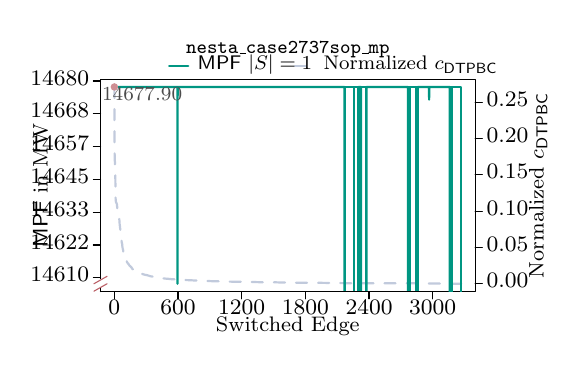
\begin{tikzpicture}[x=1pt,y=1pt]
\definecolor{fillColor}{RGB}{255,255,255}
\path[use as bounding box,fill=fillColor,fill opacity=0.00] (0,0) rectangle (440.85,271.01);
\begin{scope}
\path[clip] (  0.00,  0.00) rectangle (440.85,271.01);
\definecolor{drawColor}{RGB}{193,202,220}

\path[draw=drawColor,line width= 0.8pt,dash pattern=on 4pt off 4pt ,line join=round,line cap=round] ( 72.86,221.20) --
	( 72.95,181.25) --
	( 73.04,169.45) --
	( 73.13,159.17) --
	( 73.22,159.12) --
	( 73.31,158.42) --
	( 73.40,152.95) --
	( 73.49,151.65) --
	( 73.57,149.15) --
	( 73.66,146.86) --
	( 73.75,136.17) --
	( 73.84,129.07) --
	( 73.93,127.03) --
	( 74.02,125.48) --
	( 74.11,125.14) --
	( 74.20,124.21) --
	( 74.29,124.20) --
	( 74.38,124.19) --
	( 74.47,123.86) --
	( 74.56,123.79) --
	( 74.65,123.61) --
	( 74.73,123.37) --
	( 74.82,123.06) --
	( 74.91,122.95) --
	( 75.00,122.61) --
	( 75.09,120.87) --
	( 75.18,120.80) --
	( 75.27,119.48) --
	( 75.36,118.46) --
	( 75.45,118.39) --
	( 75.54,117.96) --
	( 75.63,117.53) --
	( 75.72,117.38) --
	( 75.80,116.01) --
	( 75.89,114.78) --
	( 75.98,114.64) --
	( 76.07,114.10) --
	( 76.16,113.64) --
	( 76.25,113.53) --
	( 76.34,112.66) --
	( 76.43,112.45) --
	( 76.52,112.33) --
	( 76.61,112.28) --
	( 76.70,111.19) --
	( 76.79,111.06) --
	( 76.88,110.77) --
	( 76.96,110.19) --
	( 77.05,109.59) --
	( 77.14,107.44) --
	( 77.23,107.09) --
	( 77.32,105.01) --
	( 77.41,104.83) --
	( 77.50,104.49) --
	( 77.59,102.74) --
	( 77.68,102.66) --
	( 77.77,102.11) --
	( 77.86,101.79) --
	( 77.95,100.32) --
	( 78.03, 98.25) --
	( 78.12, 98.11) --
	( 78.21, 97.82) --
	( 78.30, 96.67) --
	( 78.39, 95.72) --
	( 78.48, 95.26) --
	( 78.57, 93.95) --
	( 78.66, 93.69) --
	( 78.75, 92.97) --
	( 78.84, 92.12) --
	( 78.93, 91.68) --
	( 79.02, 90.40) --
	( 79.11, 90.22) --
	( 79.19, 90.07) --
	( 79.28, 89.82) --
	( 79.37, 89.30) --
	( 79.46, 88.93) --
	( 79.55, 87.39) --
	( 79.64, 86.62) --
	( 79.73, 86.59) --
	( 79.82, 85.36) --
	( 79.91, 85.10) --
	( 80.00, 84.83) --
	( 80.09, 84.77) --
	( 80.18, 84.62) --
	( 80.27, 83.01) --
	( 80.35, 82.96) --
	( 80.44, 82.58) --
	( 80.53, 82.23) --
	( 80.62, 82.20) --
	( 80.71, 80.80) --
	( 80.80, 80.54) --
	( 80.89, 80.30) --
	( 80.98, 80.20) --
	( 81.07, 80.19) --
	( 81.16, 79.99) --
	( 81.25, 79.82) --
	( 81.34, 79.72) --
	( 81.42, 79.72) --
	( 81.51, 79.46) --
	( 81.60, 79.39) --
	( 81.69, 78.30) --
	( 81.78, 78.28) --
	( 81.87, 78.08) --
	( 81.96, 77.98) --
	( 82.05, 77.92) --
	( 82.14, 77.56) --
	( 82.23, 77.55) --
	( 82.32, 77.23) --
	( 82.41, 77.00) --
	( 82.50, 76.98) --
	( 82.58, 76.47) --
	( 82.67, 76.30) --
	( 82.76, 76.14) --
	( 82.85, 76.00) --
	( 82.94, 75.90) --
	( 83.03, 75.73) --
	( 83.12, 75.32) --
	( 83.21, 75.13) --
	( 83.30, 74.54) --
	( 83.39, 74.49) --
	( 83.48, 73.69) --
	( 83.57, 73.67) --
	( 83.65, 73.66) --
	( 83.74, 73.56) --
	( 83.83, 73.54) --
	( 83.92, 73.30) --
	( 84.01, 73.13) --
	( 84.10, 73.11) --
	( 84.19, 72.87) --
	( 84.28, 72.84) --
	( 84.37, 72.76) --
	( 84.46, 72.75) --
	( 84.55, 72.67) --
	( 84.64, 72.45) --
	( 84.73, 72.33) --
	( 84.81, 72.29) --
	( 84.90, 72.22) --
	( 84.99, 72.18) --
	( 85.08, 71.69) --
	( 85.17, 71.64) --
	( 85.26, 71.59) --
	( 85.35, 71.23) --
	( 85.44, 71.22) --
	( 85.53, 71.07) --
	( 85.62, 71.00) --
	( 85.71, 70.99) --
	( 85.80, 70.92) --
	( 85.89, 70.91) --
	( 85.97, 70.80) --
	( 86.06, 70.69) --
	( 86.15, 70.65) --
	( 86.24, 70.64) --
	( 86.33, 70.38) --
	( 86.42, 70.25) --
	( 86.51, 70.24) --
	( 86.60, 70.22) --
	( 86.69, 70.10) --
	( 86.78, 69.98) --
	( 86.87, 69.95) --
	( 86.96, 69.77) --
	( 87.04, 69.67) --
	( 87.13, 69.62) --
	( 87.22, 69.48) --
	( 87.31, 69.46) --
	( 87.40, 69.31) --
	( 87.49, 68.95) --
	( 87.58, 68.88) --
	( 87.67, 68.82) --
	( 87.76, 68.68) --
	( 87.85, 68.42) --
	( 87.94, 68.41) --
	( 88.03, 68.18) --
	( 88.12, 68.12) --
	( 88.20, 68.08) --
	( 88.29, 68.05) --
	( 88.38, 68.01) --
	( 88.47, 67.94) --
	( 88.56, 67.90) --
	( 88.65, 67.90) --
	( 88.74, 67.87) --
	( 88.83, 67.69) --
	( 88.92, 67.52) --
	( 89.01, 67.50) --
	( 89.10, 67.30) --
	( 89.19, 67.15) --
	( 89.27, 67.06) --
	( 89.36, 67.00) --
	( 89.45, 66.96) --
	( 89.54, 66.92) --
	( 89.63, 66.77) --
	( 89.72, 66.77) --
	( 89.81, 66.77) --
	( 89.90, 66.72) --
	( 89.99, 66.67) --
	( 90.08, 66.61) --
	( 90.17, 66.54) --
	( 90.26, 66.49) --
	( 90.35, 66.48) --
	( 90.43, 66.43) --
	( 90.52, 66.27) --
	( 90.61, 66.26) --
	( 90.70, 66.18) --
	( 90.79, 66.14) --
	( 90.88, 66.09) --
	( 90.97, 66.06) --
	( 91.06, 66.02) --
	( 91.15, 66.00) --
	( 91.24, 65.99) --
	( 91.33, 65.84) --
	( 91.42, 65.81) --
	( 91.51, 65.79) --
	( 91.59, 65.57) --
	( 91.68, 65.55) --
	( 91.77, 65.53) --
	( 91.86, 65.53) --
	( 91.95, 65.41) --
	( 92.04, 65.36) --
	( 92.13, 65.35) --
	( 92.22, 65.30) --
	( 92.31, 65.23) --
	( 92.40, 65.08) --
	( 92.49, 65.06) --
	( 92.58, 64.95) --
	( 92.66, 64.83) --
	( 92.75, 64.78) --
	( 92.84, 64.78) --
	( 92.93, 64.76) --
	( 93.02, 64.72) --
	( 93.11, 64.71) --
	( 93.20, 64.70) --
	( 93.29, 64.67) --
	( 93.38, 64.64) --
	( 93.47, 64.63) --
	( 93.56, 64.62) --
	( 93.65, 64.62) --
	( 93.74, 64.62) --
	( 93.82, 64.60) --
	( 93.91, 64.53) --
	( 94.00, 64.51) --
	( 94.09, 64.45) --
	( 94.18, 64.45) --
	( 94.27, 64.41) --
	( 94.36, 64.41) --
	( 94.45, 64.40) --
	( 94.54, 64.40) --
	( 94.63, 64.40) --
	( 94.72, 64.39) --
	( 94.81, 64.36) --
	( 94.89, 64.36) --
	( 94.98, 64.34) --
	( 95.07, 64.33) --
	( 95.16, 64.28) --
	( 95.25, 64.27) --
	( 95.34, 64.20) --
	( 95.43, 64.18) --
	( 95.52, 64.17) --
	( 95.61, 64.16) --
	( 95.70, 64.13) --
	( 95.79, 64.11) --
	( 95.88, 64.09) --
	( 95.97, 64.04) --
	( 96.05, 64.04) --
	( 96.14, 64.03) --
	( 96.23, 64.01) --
	( 96.32, 64.00) --
	( 96.41, 63.98) --
	( 96.50, 63.97) --
	( 96.59, 63.97) --
	( 96.68, 63.93) --
	( 96.77, 63.90) --
	( 96.86, 63.88) --
	( 96.95, 63.80) --
	( 97.04, 63.79) --
	( 97.13, 63.73) --
	( 97.21, 63.70) --
	( 97.30, 63.70) --
	( 97.39, 63.68) --
	( 97.48, 63.66) --
	( 97.57, 63.65) --
	( 97.66, 63.64) --
	( 97.75, 63.62) --
	( 97.84, 63.59) --
	( 97.93, 63.55) --
	( 98.02, 63.54) --
	( 98.11, 63.48) --
	( 98.20, 63.44) --
	( 98.28, 63.44) --
	( 98.37, 63.43) --
	( 98.46, 63.36) --
	( 98.55, 63.36) --
	( 98.64, 63.32) --
	( 98.73, 63.30) --
	( 98.82, 63.29) --
	( 98.91, 63.28) --
	( 99.00, 63.26) --
	( 99.09, 63.25) --
	( 99.18, 63.23) --
	( 99.27, 63.23) --
	( 99.36, 63.21) --
	( 99.44, 63.20) --
	( 99.53, 63.18) --
	( 99.62, 63.18) --
	( 99.71, 63.16) --
	( 99.80, 63.13) --
	( 99.89, 63.10) --
	( 99.98, 63.08) --
	(100.07, 63.05) --
	(100.16, 63.02) --
	(100.25, 63.00) --
	(100.34, 62.93) --
	(100.43, 62.91) --
	(100.51, 62.91) --
	(100.60, 62.91) --
	(100.69, 62.90) --
	(100.78, 62.88) --
	(100.87, 62.87) --
	(100.96, 62.86) --
	(101.05, 62.78) --
	(101.14, 62.76) --
	(101.23, 62.71) --
	(101.32, 62.69) --
	(101.41, 62.66) --
	(101.50, 62.65) --
	(101.59, 62.65) --
	(101.67, 62.64) --
	(101.76, 62.62) --
	(101.85, 62.59) --
	(101.94, 62.57) --
	(102.03, 62.48) --
	(102.12, 62.48) --
	(102.21, 62.45) --
	(102.30, 62.45) --
	(102.39, 62.42) --
	(102.48, 62.35) --
	(102.57, 62.30) --
	(102.66, 62.26) --
	(102.74, 62.25) --
	(102.83, 62.24) --
	(102.92, 62.23) --
	(103.01, 62.19) --
	(103.10, 62.18) --
	(103.19, 62.16) --
	(103.28, 62.14) --
	(103.37, 62.11) --
	(103.46, 62.05) --
	(103.55, 62.04) --
	(103.64, 62.03) --
	(103.73, 62.02) --
	(103.82, 62.02) --
	(103.90, 62.01) --
	(103.99, 62.00) --
	(104.08, 61.99) --
	(104.17, 61.95) --
	(104.26, 61.94) --
	(104.35, 61.94) --
	(104.44, 61.86) --
	(104.53, 61.85) --
	(104.62, 61.85) --
	(104.71, 61.83) --
	(104.80, 61.83) --
	(104.89, 61.81) --
	(104.98, 61.81) --
	(105.06, 61.79) --
	(105.15, 61.74) --
	(105.24, 61.74) --
	(105.33, 61.72) --
	(105.42, 61.69) --
	(105.51, 61.66) --
	(105.60, 61.66) --
	(105.69, 61.65) --
	(105.78, 61.61) --
	(105.87, 61.60) --
	(105.96, 61.57) --
	(106.05, 61.57) --
	(106.13, 61.56) --
	(106.22, 61.56) --
	(106.31, 61.55) --
	(106.40, 61.54) --
	(106.49, 61.54) --
	(106.58, 61.53) --
	(106.67, 61.52) --
	(106.76, 61.52) --
	(106.85, 61.48) --
	(106.94, 61.47) --
	(107.03, 61.46) --
	(107.12, 61.44) --
	(107.21, 61.42) --
	(107.29, 61.42) --
	(107.38, 61.38) --
	(107.47, 61.36) --
	(107.56, 61.36) --
	(107.65, 61.33) --
	(107.74, 61.32) --
	(107.83, 61.28) --
	(107.92, 61.26) --
	(108.01, 61.24) --
	(108.10, 61.24) --
	(108.19, 61.23) --
	(108.28, 61.23) --
	(108.36, 61.23) --
	(108.45, 61.21) --
	(108.54, 61.18) --
	(108.63, 61.17) --
	(108.72, 61.17) --
	(108.81, 61.16) --
	(108.90, 61.15) --
	(108.99, 61.13) --
	(109.08, 61.11) --
	(109.17, 61.11) --
	(109.26, 61.10) --
	(109.35, 61.08) --
	(109.44, 61.07) --
	(109.52, 61.06) --
	(109.61, 61.05) --
	(109.70, 61.02) --
	(109.79, 61.01) --
	(109.88, 60.95) --
	(109.97, 60.94) --
	(110.06, 60.93) --
	(110.15, 60.92) --
	(110.24, 60.89) --
	(110.33, 60.87) --
	(110.42, 60.86) --
	(110.51, 60.83) --
	(110.60, 60.82) --
	(110.68, 60.80) --
	(110.77, 60.79) --
	(110.86, 60.76) --
	(110.95, 60.75) --
	(111.04, 60.74) --
	(111.13, 60.72) --
	(111.22, 60.71) --
	(111.31, 60.71) --
	(111.40, 60.71) --
	(111.49, 60.69) --
	(111.58, 60.68) --
	(111.67, 60.68) --
	(111.75, 60.67) --
	(111.84, 60.65) --
	(111.93, 60.62) --
	(112.02, 60.61) --
	(112.11, 60.61) --
	(112.20, 60.59) --
	(112.29, 60.58) --
	(112.38, 60.57) --
	(112.47, 60.57) --
	(112.56, 60.56) --
	(112.65, 60.56) --
	(112.74, 60.55) --
	(112.83, 60.53) --
	(112.91, 60.53) --
	(113.00, 60.53) --
	(113.09, 60.52) --
	(113.18, 60.47) --
	(113.27, 60.46) --
	(113.36, 60.44) --
	(113.45, 60.43) --
	(113.54, 60.43) --
	(113.63, 60.42) --
	(113.72, 60.41) --
	(113.81, 60.37) --
	(113.90, 60.37) --
	(113.98, 60.35) --
	(114.07, 60.35) --
	(114.16, 60.34) --
	(114.25, 60.34) --
	(114.34, 60.33) --
	(114.43, 60.30) --
	(114.52, 60.30) --
	(114.61, 60.28) --
	(114.70, 60.27) --
	(114.79, 60.25) --
	(114.88, 60.24) --
	(114.97, 60.24) --
	(115.06, 60.23) --
	(115.14, 60.23) --
	(115.23, 60.23) --
	(115.32, 60.20) --
	(115.41, 60.15) --
	(115.50, 60.14) --
	(115.59, 60.14) --
	(115.68, 60.14) --
	(115.77, 60.13) --
	(115.86, 60.12) --
	(115.95, 60.11) --
	(116.04, 60.11) --
	(116.13, 60.11) --
	(116.22, 60.10) --
	(116.30, 60.09) --
	(116.39, 60.07) --
	(116.48, 60.06) --
	(116.57, 60.06) --
	(116.66, 60.05) --
	(116.75, 60.03) --
	(116.84, 60.03) --
	(116.93, 60.02) --
	(117.02, 60.02) --
	(117.11, 60.01) --
	(117.20, 60.01) --
	(117.29, 60.00) --
	(117.37, 59.99) --
	(117.46, 59.99) --
	(117.55, 59.98) --
	(117.64, 59.98) --
	(117.73, 59.97) --
	(117.82, 59.96) --
	(117.91, 59.96) --
	(118.00, 59.95) --
	(118.09, 59.95) --
	(118.18, 59.94) --
	(118.27, 59.94) --
	(118.36, 59.92) --
	(118.45, 59.91) --
	(118.53, 59.89) --
	(118.62, 59.89) --
	(118.71, 59.87) --
	(118.80, 59.87) --
	(118.89, 59.86) --
	(118.98, 59.85) --
	(119.07, 59.84) --
	(119.16, 59.83) --
	(119.25, 59.82) --
	(119.34, 59.82) --
	(119.43, 59.81) --
	(119.52, 59.79) --
	(119.60, 59.79) --
	(119.69, 59.78) --
	(119.78, 59.75) --
	(119.87, 59.74) --
	(119.96, 59.72) --
	(120.05, 59.72) --
	(120.14, 59.72) --
	(120.23, 59.71) --
	(120.32, 59.70) --
	(120.41, 59.69) --
	(120.50, 59.69) --
	(120.59, 59.69) --
	(120.68, 59.68) --
	(120.76, 59.68) --
	(120.85, 59.67) --
	(120.94, 59.67) --
	(121.03, 59.66) --
	(121.12, 59.65) --
	(121.21, 59.65) --
	(121.30, 59.64) --
	(121.39, 59.64) --
	(121.48, 59.63) --
	(121.57, 59.63) --
	(121.66, 59.62) --
	(121.75, 59.62) --
	(121.84, 59.61) --
	(121.92, 59.61) --
	(122.01, 59.60) --
	(122.10, 59.60) --
	(122.19, 59.59) --
	(122.28, 59.59) --
	(122.37, 59.58) --
	(122.46, 59.54) --
	(122.55, 59.53) --
	(122.64, 59.53) --
	(122.73, 59.52) --
	(122.82, 59.52) --
	(122.91, 59.52) --
	(122.99, 59.52) --
	(123.08, 59.52) --
	(123.17, 59.51) --
	(123.26, 59.51) --
	(123.35, 59.49) --
	(123.44, 59.48) --
	(123.53, 59.48) --
	(123.62, 59.46) --
	(123.71, 59.45) --
	(123.80, 59.45) --
	(123.89, 59.44) --
	(123.98, 59.43) --
	(124.07, 59.43) --
	(124.15, 59.42) --
	(124.24, 59.42) --
	(124.33, 59.42) --
	(124.42, 59.41) --
	(124.51, 59.41) --
	(124.60, 59.40) --
	(124.69, 59.40) --
	(124.78, 59.40) --
	(124.87, 59.38) --
	(124.96, 59.37) --
	(125.05, 59.36) --
	(125.14, 59.34) --
	(125.22, 59.34) --
	(125.31, 59.34) --
	(125.40, 59.32) --
	(125.49, 59.31) --
	(125.58, 59.31) --
	(125.67, 59.31) --
	(125.76, 59.31) --
	(125.85, 59.30) --
	(125.94, 59.30) --
	(126.03, 59.30) --
	(126.12, 59.28) --
	(126.21, 59.28) --
	(126.30, 59.27) --
	(126.38, 59.27) --
	(126.47, 59.26) --
	(126.56, 59.26) --
	(126.65, 59.25) --
	(126.74, 59.25) --
	(126.83, 59.25) --
	(126.92, 59.25) --
	(127.01, 59.25) --
	(127.10, 59.24) --
	(127.19, 59.24) --
	(127.28, 59.24) --
	(127.37, 59.23) --
	(127.46, 59.22) --
	(127.54, 59.22) --
	(127.63, 59.22) --
	(127.72, 59.21) --
	(127.81, 59.21) --
	(127.90, 59.21) --
	(127.99, 59.21) --
	(128.08, 59.20) --
	(128.17, 59.19) --
	(128.26, 59.19) --
	(128.35, 59.17) --
	(128.44, 59.17) --
	(128.53, 59.16) --
	(128.61, 59.15) --
	(128.70, 59.15) --
	(128.79, 59.14) --
	(128.88, 59.13) --
	(128.97, 59.13) --
	(129.06, 59.13) --
	(129.15, 59.12) --
	(129.24, 59.11) --
	(129.33, 59.10) --
	(129.42, 59.10) --
	(129.51, 59.10) --
	(129.60, 59.10) --
	(129.69, 59.10) --
	(129.77, 59.08) --
	(129.86, 59.08) --
	(129.95, 59.07) --
	(130.04, 59.07) --
	(130.13, 59.06) --
	(130.22, 59.06) --
	(130.31, 59.05) --
	(130.40, 59.05) --
	(130.49, 59.05) --
	(130.58, 59.05) --
	(130.67, 59.02) --
	(130.76, 59.01) --
	(130.84, 59.01) --
	(130.93, 59.01) --
	(131.02, 59.00) --
	(131.11, 59.00) --
	(131.20, 58.99) --
	(131.29, 58.99) --
	(131.38, 58.99) --
	(131.47, 58.98) --
	(131.56, 58.98) --
	(131.65, 58.98) --
	(131.74, 58.98) --
	(131.83, 58.97) --
	(131.92, 58.97) --
	(132.00, 58.97) --
	(132.09, 58.96) --
	(132.18, 58.96) --
	(132.27, 58.96) --
	(132.36, 58.95) --
	(132.45, 58.94) --
	(132.54, 58.93) --
	(132.63, 58.93) --
	(132.72, 58.91) --
	(132.81, 58.91) --
	(132.90, 58.90) --
	(132.99, 58.89) --
	(133.08, 58.89) --
	(133.16, 58.89) --
	(133.25, 58.89) --
	(133.34, 58.88) --
	(133.43, 58.87) --
	(133.52, 58.87) --
	(133.61, 58.87) --
	(133.70, 58.87) --
	(133.79, 58.87) --
	(133.88, 58.87) --
	(133.97, 58.86) --
	(134.06, 58.86) --
	(134.15, 58.86) --
	(134.23, 58.86) --
	(134.32, 58.86) --
	(134.41, 58.86) --
	(134.50, 58.85) --
	(134.59, 58.85) --
	(134.68, 58.85) --
	(134.77, 58.85) --
	(134.86, 58.85) --
	(134.95, 58.84) --
	(135.04, 58.83) --
	(135.13, 58.83) --
	(135.22, 58.83) --
	(135.31, 58.82) --
	(135.39, 58.82) --
	(135.48, 58.82) --
	(135.57, 58.82) --
	(135.66, 58.81) --
	(135.75, 58.81) --
	(135.84, 58.80) --
	(135.93, 58.80) --
	(136.02, 58.79) --
	(136.11, 58.79) --
	(136.20, 58.78) --
	(136.29, 58.78) --
	(136.38, 58.78) --
	(136.46, 58.77) --
	(136.55, 58.77) --
	(136.64, 58.76) --
	(136.73, 58.76) --
	(136.82, 58.75) --
	(136.91, 58.75) --
	(137.00, 58.75) --
	(137.09, 58.74) --
	(137.18, 58.73) --
	(137.27, 58.73) --
	(137.36, 58.73) --
	(137.45, 58.72) --
	(137.54, 58.70) --
	(137.62, 58.70) --
	(137.71, 58.69) --
	(137.80, 58.68) --
	(137.89, 58.68) --
	(137.98, 58.68) --
	(138.07, 58.68) --
	(138.16, 58.67) --
	(138.25, 58.67) --
	(138.34, 58.67) --
	(138.43, 58.66) --
	(138.52, 58.65) --
	(138.61, 58.65) --
	(138.69, 58.65) --
	(138.78, 58.64) --
	(138.87, 58.64) --
	(138.96, 58.64) --
	(139.05, 58.63) --
	(139.14, 58.63) --
	(139.23, 58.63) --
	(139.32, 58.63) --
	(139.41, 58.62) --
	(139.50, 58.62) --
	(139.59, 58.62) --
	(139.68, 58.61) --
	(139.77, 58.61) --
	(139.85, 58.61) --
	(139.94, 58.61) --
	(140.03, 58.61) --
	(140.12, 58.60) --
	(140.21, 58.59) --
	(140.30, 58.59) --
	(140.39, 58.58) --
	(140.48, 58.58) --
	(140.57, 58.58) --
	(140.66, 58.57) --
	(140.75, 58.55) --
	(140.84, 58.54) --
	(140.93, 58.54) --
	(141.01, 58.53) --
	(141.10, 58.53) --
	(141.19, 58.53) --
	(141.28, 58.52) --
	(141.37, 58.51) --
	(141.46, 58.51) --
	(141.55, 58.51) --
	(141.64, 58.50) --
	(141.73, 58.50) --
	(141.82, 58.49) --
	(141.91, 58.48) --
	(142.00, 58.48) --
	(142.08, 58.47) --
	(142.17, 58.47) --
	(142.26, 58.47) --
	(142.35, 58.46) --
	(142.44, 58.46) --
	(142.53, 58.46) --
	(142.62, 58.45) --
	(142.71, 58.43) --
	(142.80, 58.43) --
	(142.89, 58.43) --
	(142.98, 58.42) --
	(143.07, 58.42) --
	(143.16, 58.42) --
	(143.24, 58.42) --
	(143.33, 58.41) --
	(143.42, 58.41) --
	(143.51, 58.40) --
	(143.60, 58.40) --
	(143.69, 58.40) --
	(143.78, 58.39) --
	(143.87, 58.39) --
	(143.96, 58.38) --
	(144.05, 58.38) --
	(144.14, 58.38) --
	(144.23, 58.37) --
	(144.31, 58.37) --
	(144.40, 58.37) --
	(144.49, 58.37) --
	(144.58, 58.37) --
	(144.67, 58.36) --
	(144.76, 58.36) --
	(144.85, 58.36) --
	(144.94, 58.36) --
	(145.03, 58.36) --
	(145.12, 58.35) --
	(145.21, 58.35) --
	(145.30, 58.34) --
	(145.39, 58.33) --
	(145.47, 58.32) --
	(145.56, 58.32) --
	(145.65, 58.31) --
	(145.74, 58.31) --
	(145.83, 58.31) --
	(145.92, 58.31) --
	(146.01, 58.31) --
	(146.10, 58.31) --
	(146.19, 58.30) --
	(146.28, 58.30) --
	(146.37, 58.29) --
	(146.46, 58.29) --
	(146.55, 58.29) --
	(146.63, 58.28) --
	(146.72, 58.28) --
	(146.81, 58.28) --
	(146.90, 58.27) --
	(146.99, 58.27) --
	(147.08, 58.27) --
	(147.17, 58.27) --
	(147.26, 58.26) --
	(147.35, 58.25) --
	(147.44, 58.25) --
	(147.53, 58.25) --
	(147.62, 58.24) --
	(147.70, 58.24) --
	(147.79, 58.23) --
	(147.88, 58.23) --
	(147.97, 58.23) --
	(148.06, 58.23) --
	(148.15, 58.23) --
	(148.24, 58.23) --
	(148.33, 58.22) --
	(148.42, 58.21) --
	(148.51, 58.21) --
	(148.60, 58.21) --
	(148.69, 58.21) --
	(148.78, 58.21) --
	(148.86, 58.20) --
	(148.95, 58.19) --
	(149.04, 58.19) --
	(149.13, 58.19) --
	(149.22, 58.18) --
	(149.31, 58.18) --
	(149.40, 58.18) --
	(149.49, 58.18) --
	(149.58, 58.17) --
	(149.67, 58.17) --
	(149.76, 58.16) --
	(149.85, 58.16) --
	(149.93, 58.16) --
	(150.02, 58.15) --
	(150.11, 58.15) --
	(150.20, 58.14) --
	(150.29, 58.14) --
	(150.38, 58.14) --
	(150.47, 58.14) --
	(150.56, 58.14) --
	(150.65, 58.13) --
	(150.74, 58.13) --
	(150.83, 58.13) --
	(150.92, 58.13) --
	(151.01, 58.13) --
	(151.09, 58.13) --
	(151.18, 58.13) --
	(151.27, 58.12) --
	(151.36, 58.12) --
	(151.45, 58.12) --
	(151.54, 58.12) --
	(151.63, 58.12) --
	(151.72, 58.11) --
	(151.81, 58.11) --
	(151.90, 58.11) --
	(151.99, 58.11) --
	(152.08, 58.10) --
	(152.17, 58.10) --
	(152.25, 58.09) --
	(152.34, 58.09) --
	(152.43, 58.08) --
	(152.52, 58.08) --
	(152.61, 58.08) --
	(152.70, 58.08) --
	(152.79, 58.06) --
	(152.88, 58.06) --
	(152.97, 58.06) --
	(153.06, 58.05) --
	(153.15, 58.05) --
	(153.24, 58.04) --
	(153.32, 58.03) --
	(153.41, 58.03) --
	(153.50, 58.03) --
	(153.59, 58.03) --
	(153.68, 58.02) --
	(153.77, 58.02) --
	(153.86, 58.02) --
	(153.95, 58.02) --
	(154.04, 58.01) --
	(154.13, 58.01) --
	(154.22, 58.01) --
	(154.31, 58.01) --
	(154.40, 58.00) --
	(154.48, 58.00) --
	(154.57, 57.99) --
	(154.66, 57.99) --
	(154.75, 57.99) --
	(154.84, 57.99) --
	(154.93, 57.99) --
	(155.02, 57.99) --
	(155.11, 57.99) --
	(155.20, 57.99) --
	(155.29, 57.99) --
	(155.38, 57.99) --
	(155.47, 57.99) --
	(155.55, 57.99) --
	(155.64, 57.98) --
	(155.73, 57.98) --
	(155.82, 57.98) --
	(155.91, 57.97) --
	(156.00, 57.97) --
	(156.09, 57.97) --
	(156.18, 57.97) --
	(156.27, 57.97) --
	(156.36, 57.96) --
	(156.45, 57.95) --
	(156.54, 57.95) --
	(156.63, 57.95) --
	(156.71, 57.95) --
	(156.80, 57.95) --
	(156.89, 57.95) --
	(156.98, 57.94) --
	(157.07, 57.94) --
	(157.16, 57.94) --
	(157.25, 57.94) --
	(157.34, 57.94) --
	(157.43, 57.94) --
	(157.52, 57.93) --
	(157.61, 57.93) --
	(157.70, 57.93) --
	(157.79, 57.93) --
	(157.87, 57.93) --
	(157.96, 57.93) --
	(158.05, 57.93) --
	(158.14, 57.92) --
	(158.23, 57.92) --
	(158.32, 57.92) --
	(158.41, 57.91) --
	(158.50, 57.90) --
	(158.59, 57.90) --
	(158.68, 57.90) --
	(158.77, 57.90) --
	(158.86, 57.90) --
	(158.94, 57.90) --
	(159.03, 57.90) --
	(159.12, 57.89) --
	(159.21, 57.89) --
	(159.30, 57.89) --
	(159.39, 57.89) --
	(159.48, 57.89) --
	(159.57, 57.89) --
	(159.66, 57.88) --
	(159.75, 57.88) --
	(159.84, 57.88) --
	(159.93, 57.88) --
	(160.02, 57.88) --
	(160.10, 57.88) --
	(160.19, 57.87) --
	(160.28, 57.87) --
	(160.37, 57.87) --
	(160.46, 57.86) --
	(160.55, 57.86) --
	(160.64, 57.86) --
	(160.73, 57.86) --
	(160.82, 57.86) --
	(160.91, 57.86) --
	(161.00, 57.86) --
	(161.09, 57.84) --
	(161.17, 57.84) --
	(161.26, 57.83) --
	(161.35, 57.82) --
	(161.44, 57.82) --
	(161.53, 57.82) --
	(161.62, 57.81) --
	(161.71, 57.81) --
	(161.80, 57.81) --
	(161.89, 57.81) --
	(161.98, 57.81) --
	(162.07, 57.81) --
	(162.16, 57.80) --
	(162.25, 57.79) --
	(162.33, 57.79) --
	(162.42, 57.78) --
	(162.51, 57.78) --
	(162.60, 57.78) --
	(162.69, 57.78) --
	(162.78, 57.78) --
	(162.87, 57.78) --
	(162.96, 57.77) --
	(163.05, 57.77) --
	(163.14, 57.77) --
	(163.23, 57.77) --
	(163.32, 57.77) --
	(163.41, 57.76) --
	(163.49, 57.76) --
	(163.58, 57.75) --
	(163.67, 57.75) --
	(163.76, 57.75) --
	(163.85, 57.75) --
	(163.94, 57.75) --
	(164.03, 57.75) --
	(164.12, 57.74) --
	(164.21, 57.74) --
	(164.30, 57.74) --
	(164.39, 57.74) --
	(164.48, 57.73) --
	(164.56, 57.73) --
	(164.65, 57.73) --
	(164.74, 57.73) --
	(164.83, 57.73) --
	(164.92, 57.72) --
	(165.01, 57.72) --
	(165.10, 57.72) --
	(165.19, 57.72) --
	(165.28, 57.72) --
	(165.37, 57.71) --
	(165.46, 57.71) --
	(165.55, 57.70) --
	(165.64, 57.70) --
	(165.72, 57.70) --
	(165.81, 57.70) --
	(165.90, 57.69) --
	(165.99, 57.69) --
	(166.08, 57.69) --
	(166.17, 57.69) --
	(166.26, 57.69) --
	(166.35, 57.69) --
	(166.44, 57.68) --
	(166.53, 57.68) --
	(166.62, 57.68) --
	(166.71, 57.68) --
	(166.79, 57.67) --
	(166.88, 57.67) --
	(166.97, 57.67) --
	(167.06, 57.67) --
	(167.15, 57.67) --
	(167.24, 57.67) --
	(167.33, 57.67) --
	(167.42, 57.66) --
	(167.51, 57.66) --
	(167.60, 57.66) --
	(167.69, 57.66) --
	(167.78, 57.66) --
	(167.87, 57.66) --
	(167.95, 57.66) --
	(168.04, 57.65) --
	(168.13, 57.65) --
	(168.22, 57.65) --
	(168.31, 57.65) --
	(168.40, 57.64) --
	(168.49, 57.64) --
	(168.58, 57.64) --
	(168.67, 57.64) --
	(168.76, 57.64) --
	(168.85, 57.63) --
	(168.94, 57.63) --
	(169.02, 57.63) --
	(169.11, 57.63) --
	(169.20, 57.63) --
	(169.29, 57.63) --
	(169.38, 57.62) --
	(169.47, 57.62) --
	(169.56, 57.62) --
	(169.65, 57.62) --
	(169.74, 57.61) --
	(169.83, 57.61) --
	(169.92, 57.61) --
	(170.01, 57.60) --
	(170.10, 57.60) --
	(170.18, 57.60) --
	(170.27, 57.60) --
	(170.36, 57.60) --
	(170.45, 57.60) --
	(170.54, 57.59) --
	(170.63, 57.59) --
	(170.72, 57.59) --
	(170.81, 57.59) --
	(170.90, 57.59) --
	(170.99, 57.59) --
	(171.08, 57.59) --
	(171.17, 57.59) --
	(171.26, 57.58) --
	(171.34, 57.58) --
	(171.43, 57.58) --
	(171.52, 57.57) --
	(171.61, 57.57) --
	(171.70, 57.57) --
	(171.79, 57.57) --
	(171.88, 57.56) --
	(171.97, 57.56) --
	(172.06, 57.56) --
	(172.15, 57.56) --
	(172.24, 57.55) --
	(172.33, 57.55) --
	(172.41, 57.55) --
	(172.50, 57.55) --
	(172.59, 57.55) --
	(172.68, 57.55) --
	(172.77, 57.55) --
	(172.86, 57.55) --
	(172.95, 57.55) --
	(173.04, 57.55) --
	(173.13, 57.55) --
	(173.22, 57.55) --
	(173.31, 57.55) --
	(173.40, 57.55) --
	(173.49, 57.55) --
	(173.57, 57.54) --
	(173.66, 57.54) --
	(173.75, 57.54) --
	(173.84, 57.54) --
	(173.93, 57.54) --
	(174.02, 57.54) --
	(174.11, 57.54) --
	(174.20, 57.53) --
	(174.29, 57.53) --
	(174.38, 57.53) --
	(174.47, 57.53) --
	(174.56, 57.53) --
	(174.64, 57.53) --
	(174.73, 57.53) --
	(174.82, 57.52) --
	(174.91, 57.52) --
	(175.00, 57.52) --
	(175.09, 57.52) --
	(175.18, 57.52) --
	(175.27, 57.52) --
	(175.36, 57.52) --
	(175.45, 57.52) --
	(175.54, 57.51) --
	(175.63, 57.51) --
	(175.72, 57.51) --
	(175.80, 57.51) --
	(175.89, 57.51) --
	(175.98, 57.51) --
	(176.07, 57.51) --
	(176.16, 57.50) --
	(176.25, 57.50) --
	(176.34, 57.49) --
	(176.43, 57.49) --
	(176.52, 57.49) --
	(176.61, 57.49) --
	(176.70, 57.49) --
	(176.79, 57.49) --
	(176.88, 57.49) --
	(176.96, 57.48) --
	(177.05, 57.48) --
	(177.14, 57.48) --
	(177.23, 57.48) --
	(177.32, 57.48) --
	(177.41, 57.48) --
	(177.50, 57.48) --
	(177.59, 57.47) --
	(177.68, 57.47) --
	(177.77, 57.47) --
	(177.86, 57.46) --
	(177.95, 57.46) --
	(178.03, 57.46) --
	(178.12, 57.46) --
	(178.21, 57.46) --
	(178.30, 57.46) --
	(178.39, 57.46) --
	(178.48, 57.45) --
	(178.57, 57.45) --
	(178.66, 57.45) --
	(178.75, 57.45) --
	(178.84, 57.45) --
	(178.93, 57.45) --
	(179.02, 57.45) --
	(179.11, 57.45) --
	(179.19, 57.45) --
	(179.28, 57.45) --
	(179.37, 57.45) --
	(179.46, 57.45) --
	(179.55, 57.44) --
	(179.64, 57.44) --
	(179.73, 57.44) --
	(179.82, 57.44) --
	(179.91, 57.44) --
	(180.00, 57.44) --
	(180.09, 57.44) --
	(180.18, 57.44) --
	(180.26, 57.44) --
	(180.35, 57.43) --
	(180.44, 57.43) --
	(180.53, 57.43) --
	(180.62, 57.43) --
	(180.71, 57.43) --
	(180.80, 57.43) --
	(180.89, 57.43) --
	(180.98, 57.43) --
	(181.07, 57.43) --
	(181.16, 57.43) --
	(181.25, 57.42) --
	(181.34, 57.42) --
	(181.42, 57.41) --
	(181.51, 57.41) --
	(181.60, 57.41) --
	(181.69, 57.41) --
	(181.78, 57.41) --
	(181.87, 57.41) --
	(181.96, 57.41) --
	(182.05, 57.41) --
	(182.14, 57.40) --
	(182.23, 57.40) --
	(182.32, 57.40) --
	(182.41, 57.40) --
	(182.50, 57.39) --
	(182.58, 57.39) --
	(182.67, 57.39) --
	(182.76, 57.38) --
	(182.85, 57.38) --
	(182.94, 57.38) --
	(183.03, 57.38) --
	(183.12, 57.38) --
	(183.21, 57.37) --
	(183.30, 57.36) --
	(183.39, 57.36) --
	(183.48, 57.36) --
	(183.57, 57.36) --
	(183.65, 57.36) --
	(183.74, 57.35) --
	(183.83, 57.35) --
	(183.92, 57.35) --
	(184.01, 57.35) --
	(184.10, 57.35) --
	(184.19, 57.35) --
	(184.28, 57.34) --
	(184.37, 57.34) --
	(184.46, 57.34) --
	(184.55, 57.34) --
	(184.64, 57.34) --
	(184.73, 57.34) --
	(184.81, 57.34) --
	(184.90, 57.33) --
	(184.99, 57.33) --
	(185.08, 57.33) --
	(185.17, 57.33) --
	(185.26, 57.32) --
	(185.35, 57.32) --
	(185.44, 57.32) --
	(185.53, 57.32) --
	(185.62, 57.32) --
	(185.71, 57.32) --
	(185.80, 57.32) --
	(185.88, 57.32) --
	(185.97, 57.32) --
	(186.06, 57.32) --
	(186.15, 57.31) --
	(186.24, 57.31) --
	(186.33, 57.31) --
	(186.42, 57.31) --
	(186.51, 57.30) --
	(186.60, 57.29) --
	(186.69, 57.29) --
	(186.78, 57.29) --
	(186.87, 57.29) --
	(186.96, 57.29) --
	(187.04, 57.29) --
	(187.13, 57.28) --
	(187.22, 57.28) --
	(187.31, 57.28) --
	(187.40, 57.28) --
	(187.49, 57.28) --
	(187.58, 57.28) --
	(187.67, 57.27) --
	(187.76, 57.27) --
	(187.85, 57.27) --
	(187.94, 57.27) --
	(188.03, 57.27) --
	(188.12, 57.27) --
	(188.20, 57.27) --
	(188.29, 57.27) --
	(188.38, 57.27) --
	(188.47, 57.27) --
	(188.56, 57.27) --
	(188.65, 57.27) --
	(188.74, 57.26) --
	(188.83, 57.26) --
	(188.92, 57.26) --
	(189.01, 57.25) --
	(189.10, 57.25) --
	(189.19, 57.25) --
	(189.27, 57.25) --
	(189.36, 57.25) --
	(189.45, 57.25) --
	(189.54, 57.25) --
	(189.63, 57.24) --
	(189.72, 57.24) --
	(189.81, 57.23) --
	(189.90, 57.23) --
	(189.99, 57.23) --
	(190.08, 57.23) --
	(190.17, 57.23) --
	(190.26, 57.23) --
	(190.35, 57.23) --
	(190.43, 57.23) --
	(190.52, 57.23) --
	(190.61, 57.23) --
	(190.70, 57.22) --
	(190.79, 57.22) --
	(190.88, 57.22) --
	(190.97, 57.21) --
	(191.06, 57.21) --
	(191.15, 57.21) --
	(191.24, 57.21) --
	(191.33, 57.21) --
	(191.42, 57.21) --
	(191.50, 57.21) --
	(191.59, 57.21) --
	(191.68, 57.20) --
	(191.77, 57.20) --
	(191.86, 57.20) --
	(191.95, 57.20) --
	(192.04, 57.20) --
	(192.13, 57.19) --
	(192.22, 57.19) --
	(192.31, 57.19) --
	(192.40, 57.19) --
	(192.49, 57.19) --
	(192.58, 57.19) --
	(192.66, 57.19) --
	(192.75, 57.19) --
	(192.84, 57.18) --
	(192.93, 57.18) --
	(193.02, 57.18) --
	(193.11, 57.18) --
	(193.20, 57.18) --
	(193.29, 57.17) --
	(193.38, 57.17) --
	(193.47, 57.17) --
	(193.56, 57.17) --
	(193.65, 57.17) --
	(193.74, 57.17) --
	(193.82, 57.16) --
	(193.91, 57.16) --
	(194.00, 57.16) --
	(194.09, 57.16) --
	(194.18, 57.15) --
	(194.27, 57.15) --
	(194.36, 57.15) --
	(194.45, 57.15) --
	(194.54, 57.15) --
	(194.63, 57.15) --
	(194.72, 57.15) --
	(194.81, 57.15) --
	(194.89, 57.15) --
	(194.98, 57.14) --
	(195.07, 57.14) --
	(195.16, 57.13) --
	(195.25, 57.13) --
	(195.34, 57.13) --
	(195.43, 57.13) --
	(195.52, 57.13) --
	(195.61, 57.12) --
	(195.70, 57.12) --
	(195.79, 57.12) --
	(195.88, 57.12) --
	(195.97, 57.12) --
	(196.05, 57.12) --
	(196.14, 57.12) --
	(196.23, 57.12) --
	(196.32, 57.12) --
	(196.41, 57.12) --
	(196.50, 57.12) --
	(196.59, 57.12) --
	(196.68, 57.12) --
	(196.77, 57.12) --
	(196.86, 57.12) --
	(196.95, 57.12) --
	(197.04, 57.12) --
	(197.12, 57.12) --
	(197.21, 57.12) --
	(197.30, 57.12) --
	(197.39, 57.12) --
	(197.48, 57.12) --
	(197.57, 57.12) --
	(197.66, 57.12) --
	(197.75, 57.12) --
	(197.84, 57.12) --
	(197.93, 57.12) --
	(198.02, 57.12) --
	(198.11, 57.12) --
	(198.20, 57.12) --
	(198.28, 57.12) --
	(198.37, 57.12) --
	(198.46, 57.12) --
	(198.55, 57.11) --
	(198.64, 57.11) --
	(198.73, 57.11) --
	(198.82, 57.11) --
	(198.91, 57.11) --
	(199.00, 57.11) --
	(199.09, 57.11) --
	(199.18, 57.11) --
	(199.27, 57.11) --
	(199.36, 57.11) --
	(199.44, 57.11) --
	(199.53, 57.10) --
	(199.62, 57.10) --
	(199.71, 57.10) --
	(199.80, 57.10) --
	(199.89, 57.10) --
	(199.98, 57.10) --
	(200.07, 57.10) --
	(200.16, 57.10) --
	(200.25, 57.10) --
	(200.34, 57.10) --
	(200.43, 57.10) --
	(200.51, 57.09) --
	(200.60, 57.09) --
	(200.69, 57.09) --
	(200.78, 57.09) --
	(200.87, 57.09) --
	(200.96, 57.09) --
	(201.05, 57.09) --
	(201.14, 57.09) --
	(201.23, 57.09) --
	(201.32, 57.09) --
	(201.41, 57.09) --
	(201.50, 57.09) --
	(201.59, 57.08) --
	(201.67, 57.08) --
	(201.76, 57.08) --
	(201.85, 57.08) --
	(201.94, 57.08) --
	(202.03, 57.08) --
	(202.12, 57.08) --
	(202.21, 57.08) --
	(202.30, 57.08) --
	(202.39, 57.08) --
	(202.48, 57.08) --
	(202.57, 57.08) --
	(202.66, 57.08) --
	(202.74, 57.07) --
	(202.83, 57.07) --
	(202.92, 57.07) --
	(203.01, 57.07) --
	(203.10, 57.07) --
	(203.19, 57.07) --
	(203.28, 57.06) --
	(203.37, 57.06) --
	(203.46, 57.06) --
	(203.55, 57.06) --
	(203.64, 57.06) --
	(203.73, 57.05) --
	(203.82, 57.05) --
	(203.90, 57.05) --
	(203.99, 57.05) --
	(204.08, 57.05) --
	(204.17, 57.05) --
	(204.26, 57.05) --
	(204.35, 57.05) --
	(204.44, 57.05) --
	(204.53, 57.05) --
	(204.62, 57.04) --
	(204.71, 57.04) --
	(204.80, 57.04) --
	(204.89, 57.04) --
	(204.97, 57.04) --
	(205.06, 57.04) --
	(205.15, 57.04) --
	(205.24, 57.03) --
	(205.33, 57.03) --
	(205.42, 57.03) --
	(205.51, 57.03) --
	(205.60, 57.03) --
	(205.69, 57.03) --
	(205.78, 57.03) --
	(205.87, 57.03) --
	(205.96, 57.03) --
	(206.05, 57.03) --
	(206.13, 57.03) --
	(206.22, 57.03) --
	(206.31, 57.02) --
	(206.40, 57.02) --
	(206.49, 57.02) --
	(206.58, 57.02) --
	(206.67, 57.01) --
	(206.76, 57.01) --
	(206.85, 57.01) --
	(206.94, 57.01) --
	(207.03, 57.01) --
	(207.12, 57.01) --
	(207.21, 57.01) --
	(207.29, 57.01) --
	(207.38, 57.01) --
	(207.47, 57.01) --
	(207.56, 57.01) --
	(207.65, 57.01) --
	(207.74, 57.01) --
	(207.83, 57.01) --
	(207.92, 57.00) --
	(208.01, 57.00) --
	(208.10, 57.00) --
	(208.19, 57.00) --
	(208.28, 57.00) --
	(208.36, 56.99) --
	(208.45, 56.99) --
	(208.54, 56.99) --
	(208.63, 56.99) --
	(208.72, 56.99) --
	(208.81, 56.99) --
	(208.90, 56.99) --
	(208.99, 56.99) --
	(209.08, 56.98) --
	(209.17, 56.98) --
	(209.26, 56.98) --
	(209.35, 56.98) --
	(209.44, 56.98) --
	(209.52, 56.97) --
	(209.61, 56.97) --
	(209.70, 56.97) --
	(209.79, 56.97) --
	(209.88, 56.97) --
	(209.97, 56.96) --
	(210.06, 56.96) --
	(210.15, 56.96) --
	(210.24, 56.96) --
	(210.33, 56.96) --
	(210.42, 56.96) --
	(210.51, 56.96) --
	(210.59, 56.96) --
	(210.68, 56.96) --
	(210.77, 56.95) --
	(210.86, 56.95) --
	(210.95, 56.95) --
	(211.04, 56.95) --
	(211.13, 56.95) --
	(211.22, 56.94) --
	(211.31, 56.94) --
	(211.40, 56.94) --
	(211.49, 56.94) --
	(211.58, 56.94) --
	(211.67, 56.94) --
	(211.75, 56.94) --
	(211.84, 56.93) --
	(211.93, 56.93) --
	(212.02, 56.93) --
	(212.11, 56.93) --
	(212.20, 56.92) --
	(212.29, 56.92) --
	(212.38, 56.92) --
	(212.47, 56.92) --
	(212.56, 56.92) --
	(212.65, 56.92) --
	(212.74, 56.92) --
	(212.83, 56.92) --
	(212.91, 56.91) --
	(213.00, 56.91) --
	(213.09, 56.91) --
	(213.18, 56.91) --
	(213.27, 56.91) --
	(213.36, 56.91) --
	(213.45, 56.91) --
	(213.54, 56.91) --
	(213.63, 56.91) --
	(213.72, 56.90) --
	(213.81, 56.90) --
	(213.90, 56.90) --
	(213.98, 56.90) --
	(214.07, 56.90) --
	(214.16, 56.89) --
	(214.25, 56.89) --
	(214.34, 56.89) --
	(214.43, 56.89) --
	(214.52, 56.89) --
	(214.61, 56.89) --
	(214.70, 56.89) --
	(214.79, 56.89) --
	(214.88, 56.89) --
	(214.97, 56.89) --
	(215.06, 56.88) --
	(215.14, 56.88) --
	(215.23, 56.88) --
	(215.32, 56.88) --
	(215.41, 56.88) --
	(215.50, 56.87) --
	(215.59, 56.87) --
	(215.68, 56.87) --
	(215.77, 56.87) --
	(215.86, 56.87) --
	(215.95, 56.86) --
	(216.04, 56.86) --
	(216.13, 56.86) --
	(216.21, 56.86) --
	(216.30, 56.86) --
	(216.39, 56.85) --
	(216.48, 56.85) --
	(216.57, 56.85) --
	(216.66, 56.85) --
	(216.75, 56.84) --
	(216.84, 56.84) --
	(216.93, 56.84) --
	(217.02, 56.84) --
	(217.11, 56.84) --
	(217.20, 56.84) --
	(217.29, 56.84) --
	(217.37, 56.83) --
	(217.46, 56.83) --
	(217.55, 56.83) --
	(217.64, 56.83) --
	(217.73, 56.83) --
	(217.82, 56.83) --
	(217.91, 56.83) --
	(218.00, 56.83) --
	(218.09, 56.82) --
	(218.18, 56.82) --
	(218.27, 56.82) --
	(218.36, 56.82) --
	(218.45, 56.81) --
	(218.53, 56.81) --
	(218.62, 56.81) --
	(218.71, 56.81) --
	(218.80, 56.81) --
	(218.89, 56.81) --
	(218.98, 56.81) --
	(219.07, 56.81) --
	(219.16, 56.81) --
	(219.25, 56.80) --
	(219.34, 56.80) --
	(219.43, 56.80) --
	(219.52, 56.80) --
	(219.60, 56.80) --
	(219.69, 56.80) --
	(219.78, 56.80) --
	(219.87, 56.79) --
	(219.96, 56.79) --
	(220.05, 56.79) --
	(220.14, 56.79) --
	(220.23, 56.79) --
	(220.32, 56.79) --
	(220.41, 56.78) --
	(220.50, 56.78) --
	(220.59, 56.78) --
	(220.68, 56.78) --
	(220.76, 56.78) --
	(220.85, 56.77) --
	(220.94, 56.77) --
	(221.03, 56.77) --
	(221.12, 56.77) --
	(221.21, 56.77) --
	(221.30, 56.77) --
	(221.39, 56.77) --
	(221.48, 56.77) --
	(221.57, 56.77) --
	(221.66, 56.77) --
	(221.75, 56.76) --
	(221.83, 56.76) --
	(221.92, 56.76) --
	(222.01, 56.76) --
	(222.10, 56.76) --
	(222.19, 56.76) --
	(222.28, 56.76) --
	(222.37, 56.76) --
	(222.46, 56.76) --
	(222.55, 56.76) --
	(222.64, 56.76) --
	(222.73, 56.76) --
	(222.82, 56.75) --
	(222.91, 56.75) --
	(222.99, 56.75) --
	(223.08, 56.75) --
	(223.17, 56.75) --
	(223.26, 56.75) --
	(223.35, 56.74) --
	(223.44, 56.74) --
	(223.53, 56.74) --
	(223.62, 56.74) --
	(223.71, 56.74) --
	(223.80, 56.74) --
	(223.89, 56.74) --
	(223.98, 56.74) --
	(224.07, 56.74) --
	(224.15, 56.74) --
	(224.24, 56.74) --
	(224.33, 56.74) --
	(224.42, 56.73) --
	(224.51, 56.73) --
	(224.60, 56.73) --
	(224.69, 56.73) --
	(224.78, 56.73) --
	(224.87, 56.73) --
	(224.96, 56.73) --
	(225.05, 56.73) --
	(225.14, 56.73) --
	(225.22, 56.73) --
	(225.31, 56.73) --
	(225.40, 56.73) --
	(225.49, 56.73) --
	(225.58, 56.72) --
	(225.67, 56.72) --
	(225.76, 56.72) --
	(225.85, 56.72) --
	(225.94, 56.72) --
	(226.03, 56.72) --
	(226.12, 56.72) --
	(226.21, 56.72) --
	(226.30, 56.72) --
	(226.38, 56.72) --
	(226.47, 56.72) --
	(226.56, 56.72) --
	(226.65, 56.71) --
	(226.74, 56.71) --
	(226.83, 56.71) --
	(226.92, 56.71) --
	(227.01, 56.71) --
	(227.10, 56.71) --
	(227.19, 56.71) --
	(227.28, 56.71) --
	(227.37, 56.71) --
	(227.45, 56.70) --
	(227.54, 56.70) --
	(227.63, 56.70) --
	(227.72, 56.70) --
	(227.81, 56.70) --
	(227.90, 56.70) --
	(227.99, 56.69) --
	(228.08, 56.69) --
	(228.17, 56.69) --
	(228.26, 56.69) --
	(228.35, 56.69) --
	(228.44, 56.69) --
	(228.53, 56.69) --
	(228.61, 56.69) --
	(228.70, 56.69) --
	(228.79, 56.69) --
	(228.88, 56.69) --
	(228.97, 56.69) --
	(229.06, 56.69) --
	(229.15, 56.69) --
	(229.24, 56.69) --
	(229.33, 56.69) --
	(229.42, 56.69) --
	(229.51, 56.69) --
	(229.60, 56.69) --
	(229.69, 56.69) --
	(229.77, 56.69) --
	(229.86, 56.69) --
	(229.95, 56.69) --
	(230.04, 56.69) --
	(230.13, 56.69) --
	(230.22, 56.69) --
	(230.31, 56.68) --
	(230.40, 56.68) --
	(230.49, 56.68) --
	(230.58, 56.68) --
	(230.67, 56.68) --
	(230.76, 56.68) --
	(230.84, 56.68) --
	(230.93, 56.68) --
	(231.02, 56.68) --
	(231.11, 56.68) --
	(231.20, 56.68) --
	(231.29, 56.68) --
	(231.38, 56.68) --
	(231.47, 56.68) --
	(231.56, 56.68) --
	(231.65, 56.68) --
	(231.74, 56.68) --
	(231.83, 56.68) --
	(231.92, 56.68) --
	(232.00, 56.68) --
	(232.09, 56.68) --
	(232.18, 56.68) --
	(232.27, 56.68) --
	(232.36, 56.68) --
	(232.45, 56.68) --
	(232.54, 56.68) --
	(232.63, 56.68) --
	(232.72, 56.68) --
	(232.81, 56.68) --
	(232.90, 56.68) --
	(232.99, 56.68) --
	(233.07, 56.68) --
	(233.16, 56.68) --
	(233.25, 56.68) --
	(233.34, 56.68) --
	(233.43, 56.68) --
	(233.52, 56.68) --
	(233.61, 56.67) --
	(233.70, 56.67) --
	(233.79, 56.67) --
	(233.88, 56.67) --
	(233.97, 56.67) --
	(234.06, 56.67) --
	(234.15, 56.67) --
	(234.23, 56.67) --
	(234.32, 56.67) --
	(234.41, 56.67) --
	(234.50, 56.67) --
	(234.59, 56.67) --
	(234.68, 56.67) --
	(234.77, 56.67) --
	(234.86, 56.67) --
	(234.95, 56.67) --
	(235.04, 56.67) --
	(235.13, 56.67) --
	(235.22, 56.67) --
	(235.31, 56.66) --
	(235.39, 56.66) --
	(235.48, 56.66) --
	(235.57, 56.66) --
	(235.66, 56.66) --
	(235.75, 56.66) --
	(235.84, 56.66) --
	(235.93, 56.66) --
	(236.02, 56.66) --
	(236.11, 56.66) --
	(236.20, 56.66) --
	(236.29, 56.66) --
	(236.38, 56.66) --
	(236.46, 56.66) --
	(236.55, 56.66) --
	(236.64, 56.65) --
	(236.73, 56.65) --
	(236.82, 56.65) --
	(236.91, 56.65) --
	(237.00, 56.65) --
	(237.09, 56.65) --
	(237.18, 56.65) --
	(237.27, 56.65) --
	(237.36, 56.65) --
	(237.45, 56.65) --
	(237.54, 56.65) --
	(237.62, 56.65) --
	(237.71, 56.65) --
	(237.80, 56.65) --
	(237.89, 56.65) --
	(237.98, 56.65) --
	(238.07, 56.65) --
	(238.16, 56.65) --
	(238.25, 56.65) --
	(238.34, 56.65) --
	(238.43, 56.65) --
	(238.52, 56.65) --
	(238.61, 56.65) --
	(238.69, 56.65) --
	(238.78, 56.65) --
	(238.87, 56.64) --
	(238.96, 56.64) --
	(239.05, 56.64) --
	(239.14, 56.64) --
	(239.23, 56.64) --
	(239.32, 56.64) --
	(239.41, 56.64) --
	(239.50, 56.64) --
	(239.59, 56.64) --
	(239.68, 56.64) --
	(239.77, 56.64) --
	(239.85, 56.64) --
	(239.94, 56.63) --
	(240.03, 56.63) --
	(240.12, 56.63) --
	(240.21, 56.63) --
	(240.30, 56.63) --
	(240.39, 56.63) --
	(240.48, 56.63) --
	(240.57, 56.63) --
	(240.66, 56.63) --
	(240.75, 56.63) --
	(240.84, 56.63) --
	(240.92, 56.63) --
	(241.01, 56.63) --
	(241.10, 56.63) --
	(241.19, 56.63) --
	(241.28, 56.63) --
	(241.37, 56.63) --
	(241.46, 56.62) --
	(241.55, 56.62) --
	(241.64, 56.62) --
	(241.73, 56.62) --
	(241.82, 56.62) --
	(241.91, 56.62) --
	(242.00, 56.62) --
	(242.08, 56.62) --
	(242.17, 56.62) --
	(242.26, 56.62) --
	(242.35, 56.62) --
	(242.44, 56.61) --
	(242.53, 56.61) --
	(242.62, 56.61) --
	(242.71, 56.61) --
	(242.80, 56.61) --
	(242.89, 56.61) --
	(242.98, 56.61) --
	(243.07, 56.61) --
	(243.16, 56.61) --
	(243.24, 56.61) --
	(243.33, 56.61) --
	(243.42, 56.61) --
	(243.51, 56.60) --
	(243.60, 56.60) --
	(243.69, 56.60) --
	(243.78, 56.60) --
	(243.87, 56.60) --
	(243.96, 56.60) --
	(244.05, 56.60) --
	(244.14, 56.60) --
	(244.23, 56.60) --
	(244.31, 56.60) --
	(244.40, 56.59) --
	(244.49, 56.59) --
	(244.58, 56.59) --
	(244.67, 56.59) --
	(244.76, 56.59) --
	(244.85, 56.59) --
	(244.94, 56.59) --
	(245.03, 56.59) --
	(245.12, 56.59) --
	(245.21, 56.59) --
	(245.30, 56.59) --
	(245.39, 56.59) --
	(245.47, 56.58) --
	(245.56, 56.58) --
	(245.65, 56.58) --
	(245.74, 56.58) --
	(245.83, 56.58) --
	(245.92, 56.58) --
	(246.01, 56.58) --
	(246.10, 56.58) --
	(246.19, 56.58) --
	(246.28, 56.58) --
	(246.37, 56.58) --
	(246.46, 56.58) --
	(246.54, 56.57) --
	(246.63, 56.57) --
	(246.72, 56.57) --
	(246.81, 56.57) --
	(246.90, 56.57) --
	(246.99, 56.57) --
	(247.08, 56.57) --
	(247.17, 56.57) --
	(247.26, 56.57) --
	(247.35, 56.57) --
	(247.44, 56.57) --
	(247.53, 56.57) --
	(247.62, 56.57) --
	(247.70, 56.56) --
	(247.79, 56.56) --
	(247.88, 56.56) --
	(247.97, 56.56) --
	(248.06, 56.56) --
	(248.15, 56.56) --
	(248.24, 56.56) --
	(248.33, 56.56) --
	(248.42, 56.56) --
	(248.51, 56.56) --
	(248.60, 56.55) --
	(248.69, 56.55) --
	(248.78, 56.55) --
	(248.86, 56.55) --
	(248.95, 56.55) --
	(249.04, 56.55) --
	(249.13, 56.55) --
	(249.22, 56.55) --
	(249.31, 56.55) --
	(249.40, 56.55) --
	(249.49, 56.55) --
	(249.58, 56.55) --
	(249.67, 56.54) --
	(249.76, 56.54) --
	(249.85, 56.54) --
	(249.93, 56.54) --
	(250.02, 56.54) --
	(250.11, 56.54) --
	(250.20, 56.54) --
	(250.29, 56.54) --
	(250.38, 56.54) --
	(250.47, 56.53) --
	(250.56, 56.53) --
	(250.65, 56.53) --
	(250.74, 56.53) --
	(250.83, 56.53) --
	(250.92, 56.53) --
	(251.01, 56.53) --
	(251.09, 56.53) --
	(251.18, 56.53) --
	(251.27, 56.52) --
	(251.36, 56.52) --
	(251.45, 56.52) --
	(251.54, 56.52) --
	(251.63, 56.52) --
	(251.72, 56.51) --
	(251.81, 56.51) --
	(251.90, 56.51) --
	(251.99, 56.51) --
	(252.08, 56.51) --
	(252.16, 56.51) --
	(252.25, 56.51) --
	(252.34, 56.51) --
	(252.43, 56.51) --
	(252.52, 56.51) --
	(252.61, 56.51) --
	(252.70, 56.51) --
	(252.79, 56.50) --
	(252.88, 56.50) --
	(252.97, 56.50) --
	(253.06, 56.50) --
	(253.15, 56.50) --
	(253.24, 56.50) --
	(253.32, 56.50) --
	(253.41, 56.49) --
	(253.50, 56.49) --
	(253.59, 56.49) --
	(253.68, 56.49) --
	(253.77, 56.49) --
	(253.86, 56.49) --
	(253.95, 56.49) --
	(254.04, 56.49) --
	(254.13, 56.48) --
	(254.22, 56.48) --
	(254.31, 56.48) --
	(254.40, 56.48) --
	(254.48, 56.48) --
	(254.57, 56.48) --
	(254.66, 56.48) --
	(254.75, 56.48) --
	(254.84, 56.48) --
	(254.93, 56.48) --
	(255.02, 56.48) --
	(255.11, 56.48) --
	(255.20, 56.47) --
	(255.29, 56.47) --
	(255.38, 56.47) --
	(255.47, 56.47) --
	(255.55, 56.47) --
	(255.64, 56.47) --
	(255.73, 56.47) --
	(255.82, 56.47) --
	(255.91, 56.47) --
	(256.00, 56.46) --
	(256.09, 56.46) --
	(256.18, 56.46) --
	(256.27, 56.46) --
	(256.36, 56.46) --
	(256.45, 56.46) --
	(256.54, 56.45) --
	(256.63, 56.45) --
	(256.71, 56.45) --
	(256.80, 56.45) --
	(256.89, 56.45) --
	(256.98, 56.45) --
	(257.07, 56.45) --
	(257.16, 56.45) --
	(257.25, 56.45) --
	(257.34, 56.44) --
	(257.43, 56.44) --
	(257.52, 56.44) --
	(257.61, 56.44) --
	(257.70, 56.44) --
	(257.78, 56.43) --
	(257.87, 56.43) --
	(257.96, 56.43) --
	(258.05, 56.43) --
	(258.14, 56.43) --
	(258.23, 56.43) --
	(258.32, 56.43) --
	(258.41, 56.42) --
	(258.50, 56.42) --
	(258.59, 56.42) --
	(258.68, 56.42) --
	(258.77, 56.42) --
	(258.86, 56.41) --
	(258.94, 56.41) --
	(259.03, 56.41) --
	(259.12, 56.41) --
	(259.21, 56.41) --
	(259.30, 56.41) --
	(259.39, 56.41) --
	(259.48, 56.41) --
	(259.57, 56.40) --
	(259.66, 56.40) --
	(259.75, 56.40) --
	(259.84, 56.40) --
	(259.93, 56.40) --
	(260.02, 56.40) --
	(260.10, 56.40) --
	(260.19, 56.39) --
	(260.28, 56.39) --
	(260.37, 56.39) --
	(260.46, 56.39) --
	(260.55, 56.39) --
	(260.64, 56.39) --
	(260.73, 56.39) --
	(260.82, 56.39) --
	(260.91, 56.38) --
	(261.00, 56.38) --
	(261.09, 56.38) --
	(261.17, 56.38) --
	(261.26, 56.38) --
	(261.35, 56.38) --
	(261.44, 56.38) --
	(261.53, 56.38) --
	(261.62, 56.38) --
	(261.71, 56.37) --
	(261.80, 56.37) --
	(261.89, 56.37) --
	(261.98, 56.37) --
	(262.07, 56.37) --
	(262.16, 56.37) --
	(262.25, 56.36) --
	(262.33, 56.36) --
	(262.42, 56.36) --
	(262.51, 56.36) --
	(262.60, 56.36) --
	(262.69, 56.36) --
	(262.78, 56.36) --
	(262.87, 56.36) --
	(262.96, 56.36) --
	(263.05, 56.36) --
	(263.14, 56.35) --
	(263.23, 56.35) --
	(263.32, 56.35) --
	(263.40, 56.35) --
	(263.49, 56.35) --
	(263.58, 56.35) --
	(263.67, 56.35) --
	(263.76, 56.35) --
	(263.85, 56.35) --
	(263.94, 56.35) --
	(264.03, 56.35) --
	(264.12, 56.35) --
	(264.21, 56.35) --
	(264.30, 56.35) --
	(264.39, 56.34) --
	(264.48, 56.34) --
	(264.56, 56.34) --
	(264.65, 56.34) --
	(264.74, 56.34) --
	(264.83, 56.34) --
	(264.92, 56.34) --
	(265.01, 56.34) --
	(265.10, 56.34) --
	(265.19, 56.33) --
	(265.28, 56.33) --
	(265.37, 56.33) --
	(265.46, 56.33) --
	(265.55, 56.33) --
	(265.64, 56.33) --
	(265.72, 56.33) --
	(265.81, 56.33) --
	(265.90, 56.33) --
	(265.99, 56.32) --
	(266.08, 56.32) --
	(266.17, 56.32) --
	(266.26, 56.32) --
	(266.35, 56.32) --
	(266.44, 56.32) --
	(266.53, 56.32) --
	(266.62, 56.31) --
	(266.71, 56.31) --
	(266.79, 56.31) --
	(266.88, 56.31) --
	(266.97, 56.31) --
	(267.06, 56.31) --
	(267.15, 56.31) --
	(267.24, 56.31) --
	(267.33, 56.31) --
	(267.42, 56.31) --
	(267.51, 56.31) --
	(267.60, 56.31) --
	(267.69, 56.31) --
	(267.78, 56.31) --
	(267.87, 56.31) --
	(267.95, 56.31) --
	(268.04, 56.31) --
	(268.13, 56.31) --
	(268.22, 56.30) --
	(268.31, 56.30) --
	(268.40, 56.30) --
	(268.49, 56.30) --
	(268.58, 56.30) --
	(268.67, 56.29) --
	(268.76, 56.29) --
	(268.85, 56.29) --
	(268.94, 56.29) --
	(269.02, 56.29) --
	(269.11, 56.29) --
	(269.20, 56.29) --
	(269.29, 56.28) --
	(269.38, 56.28) --
	(269.47, 56.28) --
	(269.56, 56.28) --
	(269.65, 56.28) --
	(269.74, 56.28) --
	(269.83, 56.28) --
	(269.92, 56.28) --
	(270.01, 56.28) --
	(270.10, 56.28) --
	(270.18, 56.28) --
	(270.27, 56.28) --
	(270.36, 56.28) --
	(270.45, 56.28) --
	(270.54, 56.28) --
	(270.63, 56.28) --
	(270.72, 56.28) --
	(270.81, 56.27) --
	(270.90, 56.27) --
	(270.99, 56.27) --
	(271.08, 56.27) --
	(271.17, 56.27) --
	(271.26, 56.27) --
	(271.34, 56.27) --
	(271.43, 56.27) --
	(271.52, 56.27) --
	(271.61, 56.27) --
	(271.70, 56.27) --
	(271.79, 56.27) --
	(271.88, 56.27) --
	(271.97, 56.26) --
	(272.06, 56.26) --
	(272.15, 56.26) --
	(272.24, 56.26) --
	(272.33, 56.26) --
	(272.41, 56.26) --
	(272.50, 56.26) --
	(272.59, 56.26) --
	(272.68, 56.26) --
	(272.77, 56.26) --
	(272.86, 56.26) --
	(272.95, 56.26) --
	(273.04, 56.26) --
	(273.13, 56.26) --
	(273.22, 56.26) --
	(273.31, 56.26) --
	(273.40, 56.26) --
	(273.49, 56.26) --
	(273.57, 56.26) --
	(273.66, 56.26) --
	(273.75, 56.26) --
	(273.84, 56.26) --
	(273.93, 56.26) --
	(274.02, 56.26) --
	(274.11, 56.26) --
	(274.20, 56.26) --
	(274.29, 56.26) --
	(274.38, 56.26) --
	(274.47, 56.26) --
	(274.56, 56.26) --
	(274.64, 56.26) --
	(274.73, 56.26) --
	(274.82, 56.26) --
	(274.91, 56.26) --
	(275.00, 56.26) --
	(275.09, 56.26) --
	(275.18, 56.26) --
	(275.27, 56.26) --
	(275.36, 56.26) --
	(275.45, 56.26) --
	(275.54, 56.26) --
	(275.63, 56.25) --
	(275.72, 56.25) --
	(275.80, 56.25) --
	(275.89, 56.25) --
	(275.98, 56.25) --
	(276.07, 56.25) --
	(276.16, 56.25) --
	(276.25, 56.25) --
	(276.34, 56.25) --
	(276.43, 56.25) --
	(276.52, 56.25) --
	(276.61, 56.25) --
	(276.70, 56.25) --
	(276.79, 56.25) --
	(276.87, 56.25) --
	(276.96, 56.25) --
	(277.05, 56.25) --
	(277.14, 56.25) --
	(277.23, 56.25) --
	(277.32, 56.25) --
	(277.41, 56.25) --
	(277.50, 56.25) --
	(277.59, 56.25) --
	(277.68, 56.25) --
	(277.77, 56.25) --
	(277.86, 56.25) --
	(277.95, 56.25) --
	(278.03, 56.25) --
	(278.12, 56.25) --
	(278.21, 56.25) --
	(278.30, 56.25) --
	(278.39, 56.25) --
	(278.48, 56.25) --
	(278.57, 56.25) --
	(278.66, 56.25) --
	(278.75, 56.25) --
	(278.84, 56.25) --
	(278.93, 56.25) --
	(279.02, 56.25) --
	(279.11, 56.25) --
	(279.19, 56.25) --
	(279.28, 56.25) --
	(279.37, 56.25) --
	(279.46, 56.25) --
	(279.55, 56.25) --
	(279.64, 56.25) --
	(279.73, 56.25) --
	(279.82, 56.25) --
	(279.91, 56.25) --
	(280.00, 56.25) --
	(280.09, 56.25) --
	(280.18, 56.25) --
	(280.26, 56.25) --
	(280.35, 56.25) --
	(280.44, 56.25) --
	(280.53, 56.25) --
	(280.62, 56.25) --
	(280.71, 56.25) --
	(280.80, 56.25) --
	(280.89, 56.25) --
	(280.98, 56.25) --
	(281.07, 56.25) --
	(281.16, 56.25) --
	(281.25, 56.25) --
	(281.34, 56.25) --
	(281.42, 56.25) --
	(281.51, 56.25) --
	(281.60, 56.25) --
	(281.69, 56.25) --
	(281.78, 56.25) --
	(281.87, 56.25) --
	(281.96, 56.25) --
	(282.05, 56.25) --
	(282.14, 56.25) --
	(282.23, 56.25) --
	(282.32, 56.25) --
	(282.41, 56.25) --
	(282.49, 56.25) --
	(282.58, 56.25) --
	(282.67, 56.25) --
	(282.76, 56.25) --
	(282.85, 56.25) --
	(282.94, 56.25) --
	(283.03, 56.25) --
	(283.12, 56.25) --
	(283.21, 56.25) --
	(283.30, 56.25) --
	(283.39, 56.25) --
	(283.48, 56.25) --
	(283.57, 56.25) --
	(283.65, 56.25) --
	(283.74, 56.25) --
	(283.83, 56.25) --
	(283.92, 56.25) --
	(284.01, 56.25) --
	(284.10, 56.25) --
	(284.19, 56.25) --
	(284.28, 56.25) --
	(284.37, 56.25) --
	(284.46, 56.25) --
	(284.55, 56.25) --
	(284.64, 56.25) --
	(284.73, 56.25) --
	(284.81, 56.25) --
	(284.90, 56.25) --
	(284.99, 56.25) --
	(285.08, 56.25) --
	(285.17, 56.25) --
	(285.26, 56.25) --
	(285.35, 56.25) --
	(285.44, 56.25) --
	(285.53, 56.25) --
	(285.62, 56.25) --
	(285.71, 56.25) --
	(285.80, 56.25) --
	(285.88, 56.25) --
	(285.97, 56.25) --
	(286.06, 56.25) --
	(286.15, 56.25) --
	(286.24, 56.25) --
	(286.33, 56.25) --
	(286.42, 56.25) --
	(286.51, 56.25) --
	(286.60, 56.25) --
	(286.69, 56.25) --
	(286.78, 56.25) --
	(286.87, 56.25) --
	(286.96, 56.25) --
	(287.04, 56.25) --
	(287.13, 56.25) --
	(287.22, 56.25) --
	(287.31, 56.25) --
	(287.40, 56.25) --
	(287.49, 56.25) --
	(287.58, 56.25) --
	(287.67, 56.25) --
	(287.76, 56.25) --
	(287.85, 56.25) --
	(287.94, 56.25) --
	(288.03, 56.25) --
	(288.11, 56.25) --
	(288.20, 56.25) --
	(288.29, 56.25) --
	(288.38, 56.25) --
	(288.47, 56.25) --
	(288.56, 56.25) --
	(288.65, 56.25) --
	(288.74, 56.25) --
	(288.83, 56.25) --
	(288.92, 56.25) --
	(289.01, 56.25) --
	(289.10, 56.25) --
	(289.19, 56.25) --
	(289.27, 56.25) --
	(289.36, 56.25) --
	(289.45, 56.25) --
	(289.54, 56.25) --
	(289.63, 56.25) --
	(289.72, 56.25) --
	(289.81, 56.25) --
	(289.90, 56.25) --
	(289.99, 56.25) --
	(290.08, 56.25) --
	(290.17, 56.25) --
	(290.26, 56.25) --
	(290.35, 56.25) --
	(290.43, 56.25) --
	(290.52, 56.25) --
	(290.61, 56.25) --
	(290.70, 56.25) --
	(290.79, 56.25) --
	(290.88, 56.25) --
	(290.97, 56.25) --
	(291.06, 56.25) --
	(291.15, 56.25) --
	(291.24, 56.25) --
	(291.33, 56.25) --
	(291.42, 56.25) --
	(291.50, 56.25) --
	(291.59, 56.25) --
	(291.68, 56.25) --
	(291.77, 56.25) --
	(291.86, 56.25) --
	(291.95, 56.25) --
	(292.04, 56.25) --
	(292.13, 56.25) --
	(292.22, 56.25) --
	(292.31, 56.25) --
	(292.40, 56.25) --
	(292.49, 56.25) --
	(292.58, 56.25) --
	(292.66, 56.25) --
	(292.75, 56.25) --
	(292.84, 56.25) --
	(292.93, 56.25) --
	(293.02, 56.25) --
	(293.11, 56.25) --
	(293.20, 56.25) --
	(293.29, 56.25) --
	(293.38, 56.25) --
	(293.47, 56.25) --
	(293.56, 56.25) --
	(293.65, 56.25) --
	(293.73, 56.25) --
	(293.82, 56.25) --
	(293.91, 56.25) --
	(294.00, 56.25) --
	(294.09, 56.25) --
	(294.18, 56.25) --
	(294.27, 56.25) --
	(294.36, 56.25) --
	(294.45, 56.25) --
	(294.54, 56.25) --
	(294.63, 56.25) --
	(294.72, 56.25) --
	(294.81, 56.25) --
	(294.89, 56.25) --
	(294.98, 56.25) --
	(295.07, 56.25) --
	(295.16, 56.25) --
	(295.25, 56.25) --
	(295.34, 56.25) --
	(295.43, 56.25) --
	(295.52, 56.25) --
	(295.61, 56.25) --
	(295.70, 56.25) --
	(295.79, 56.25) --
	(295.88, 56.25) --
	(295.97, 56.25) --
	(296.05, 56.25) --
	(296.14, 56.25) --
	(296.23, 56.25) --
	(296.32, 56.25) --
	(296.41, 56.25) --
	(296.50, 56.25) --
	(296.59, 56.25) --
	(296.68, 56.25) --
	(296.77, 56.25) --
	(296.86, 56.25) --
	(296.95, 56.25) --
	(297.04, 56.25) --
	(297.12, 56.25) --
	(297.21, 56.25) --
	(297.30, 56.25) --
	(297.39, 56.25) --
	(297.48, 56.25) --
	(297.57, 56.25) --
	(297.66, 56.25) --
	(297.75, 56.25) --
	(297.84, 56.25) --
	(297.93, 56.25) --
	(298.02, 56.25) --
	(298.11, 56.25) --
	(298.20, 56.25) --
	(298.28, 56.25) --
	(298.37, 56.25) --
	(298.46, 56.25) --
	(298.55, 56.25) --
	(298.64, 56.25) --
	(298.73, 56.25) --
	(298.82, 56.25) --
	(298.91, 56.25) --
	(299.00, 56.25) --
	(299.09, 56.25) --
	(299.18, 56.25) --
	(299.27, 56.25) --
	(299.35, 56.25) --
	(299.44, 56.25) --
	(299.53, 56.25) --
	(299.62, 56.25) --
	(299.71, 56.25) --
	(299.80, 56.25) --
	(299.89, 56.25) --
	(299.98, 56.25) --
	(300.07, 56.25) --
	(300.16, 56.25) --
	(300.25, 56.25) --
	(300.34, 56.25) --
	(300.43, 56.25) --
	(300.51, 56.25) --
	(300.60, 56.25) --
	(300.69, 56.25) --
	(300.78, 56.25) --
	(300.87, 56.25) --
	(300.96, 56.25) --
	(301.05, 56.25) --
	(301.14, 56.25) --
	(301.23, 56.25) --
	(301.32, 56.25) --
	(301.41, 56.25) --
	(301.50, 56.25) --
	(301.59, 56.25) --
	(301.67, 56.25) --
	(301.76, 56.25) --
	(301.85, 56.25) --
	(301.94, 56.25) --
	(302.03, 56.25) --
	(302.12, 56.25) --
	(302.21, 56.25) --
	(302.30, 56.25) --
	(302.39, 56.25) --
	(302.48, 56.25) --
	(302.57, 56.25) --
	(302.66, 56.25) --
	(302.74, 56.25) --
	(302.83, 56.25) --
	(302.92, 56.25) --
	(303.01, 56.25) --
	(303.10, 56.25) --
	(303.19, 56.25) --
	(303.28, 56.25) --
	(303.37, 56.25) --
	(303.46, 56.25) --
	(303.55, 56.25) --
	(303.64, 56.25) --
	(303.73, 56.25) --
	(303.82, 56.25) --
	(303.90, 56.25) --
	(303.99, 56.25) --
	(304.08, 56.25) --
	(304.17, 56.25) --
	(304.26, 56.25) --
	(304.35, 56.25) --
	(304.44, 56.25) --
	(304.53, 56.25) --
	(304.62, 56.25) --
	(304.71, 56.25) --
	(304.80, 56.25) --
	(304.89, 56.25) --
	(304.97, 56.25) --
	(305.06, 56.25) --
	(305.15, 56.25) --
	(305.24, 56.25) --
	(305.33, 56.25) --
	(305.42, 56.25) --
	(305.51, 56.25) --
	(305.60, 56.25) --
	(305.69, 56.25) --
	(305.78, 56.24) --
	(305.87, 56.24) --
	(305.96, 56.24) --
	(306.05, 56.24) --
	(306.13, 56.24) --
	(306.22, 56.24) --
	(306.31, 56.24) --
	(306.40, 56.24) --
	(306.49, 56.24) --
	(306.58, 56.24) --
	(306.67, 56.24) --
	(306.76, 56.24) --
	(306.85, 56.24) --
	(306.94, 56.24) --
	(307.03, 56.24) --
	(307.12, 56.24) --
	(307.20, 56.24) --
	(307.29, 56.24) --
	(307.38, 56.24) --
	(307.47, 56.24) --
	(307.56, 56.24) --
	(307.65, 56.24) --
	(307.74, 56.24) --
	(307.83, 56.24) --
	(307.92, 56.24) --
	(308.01, 56.24) --
	(308.10, 56.24) --
	(308.19, 56.24) --
	(308.28, 56.24) --
	(308.36, 56.24) --
	(308.45, 56.24) --
	(308.54, 56.24) --
	(308.63, 56.24) --
	(308.72, 56.24) --
	(308.81, 56.24) --
	(308.90, 56.24) --
	(308.99, 56.24) --
	(309.08, 56.24) --
	(309.17, 56.24) --
	(309.26, 56.24) --
	(309.35, 56.24) --
	(309.44, 56.24) --
	(309.52, 56.24) --
	(309.61, 56.24) --
	(309.70, 56.24) --
	(309.79, 56.24) --
	(309.88, 56.24) --
	(309.97, 56.24) --
	(310.06, 56.24) --
	(310.15, 56.24) --
	(310.24, 56.24) --
	(310.33, 56.24) --
	(310.42, 56.24) --
	(310.51, 56.24) --
	(310.59, 56.24) --
	(310.68, 56.24) --
	(310.77, 56.24) --
	(310.86, 56.24) --
	(310.95, 56.24) --
	(311.04, 56.24) --
	(311.13, 56.24) --
	(311.22, 56.24) --
	(311.31, 56.24) --
	(311.40, 56.24) --
	(311.49, 56.24) --
	(311.58, 56.24) --
	(311.67, 56.24) --
	(311.75, 56.24) --
	(311.84, 56.24) --
	(311.93, 56.24) --
	(312.02, 56.24) --
	(312.11, 56.24) --
	(312.20, 56.24) --
	(312.29, 56.24) --
	(312.38, 56.23) --
	(312.47, 56.23) --
	(312.56, 56.23) --
	(312.65, 56.23) --
	(312.74, 56.23) --
	(312.82, 56.23) --
	(312.91, 56.23) --
	(313.00, 56.23) --
	(313.09, 56.23) --
	(313.18, 56.23) --
	(313.27, 56.23) --
	(313.36, 56.23) --
	(313.45, 56.23) --
	(313.54, 56.23) --
	(313.63, 56.23) --
	(313.72, 56.23) --
	(313.81, 56.23) --
	(313.90, 56.23) --
	(313.98, 56.23) --
	(314.07, 56.23) --
	(314.16, 56.23) --
	(314.25, 56.23) --
	(314.34, 56.23) --
	(314.43, 56.23) --
	(314.52, 56.23) --
	(314.61, 56.23) --
	(314.70, 56.23) --
	(314.79, 56.23) --
	(314.88, 56.23) --
	(314.97, 56.23) --
	(315.06, 56.23) --
	(315.14, 56.23) --
	(315.23, 56.23) --
	(315.32, 56.23) --
	(315.41, 56.23) --
	(315.50, 56.23) --
	(315.59, 56.23) --
	(315.68, 56.23) --
	(315.77, 56.23) --
	(315.86, 56.23) --
	(315.95, 56.23) --
	(316.04, 56.23) --
	(316.13, 56.23) --
	(316.21, 56.23) --
	(316.30, 56.23) --
	(316.39, 56.23) --
	(316.48, 56.23) --
	(316.57, 56.23) --
	(316.66, 56.22) --
	(316.75, 56.22) --
	(316.84, 56.22) --
	(316.93, 56.22) --
	(317.02, 56.22) --
	(317.11, 56.22) --
	(317.20, 56.22) --
	(317.29, 56.22) --
	(317.37, 56.22) --
	(317.46, 56.22) --
	(317.55, 56.22) --
	(317.64, 56.22) --
	(317.73, 56.22) --
	(317.82, 56.22) --
	(317.91, 56.22) --
	(318.00, 56.22) --
	(318.09, 56.22) --
	(318.18, 56.22) --
	(318.27, 56.22) --
	(318.36, 56.22) --
	(318.44, 56.22) --
	(318.53, 56.22) --
	(318.62, 56.22) --
	(318.71, 56.22) --
	(318.80, 56.22) --
	(318.89, 56.22) --
	(318.98, 56.22) --
	(319.07, 56.22) --
	(319.16, 56.22) --
	(319.25, 56.22) --
	(319.34, 56.22) --
	(319.43, 56.22) --
	(319.52, 56.22) --
	(319.60, 56.22) --
	(319.69, 56.22) --
	(319.78, 56.22) --
	(319.87, 56.22) --
	(319.96, 56.22) --
	(320.05, 56.22) --
	(320.14, 56.22) --
	(320.23, 56.22) --
	(320.32, 56.22) --
	(320.41, 56.22) --
	(320.50, 56.22) --
	(320.59, 56.22) --
	(320.68, 56.22) --
	(320.76, 56.21) --
	(320.85, 56.21) --
	(320.94, 56.21) --
	(321.03, 56.21) --
	(321.12, 56.21) --
	(321.21, 56.21) --
	(321.30, 56.21) --
	(321.39, 56.21) --
	(321.48, 56.21) --
	(321.57, 56.21) --
	(321.66, 56.21) --
	(321.75, 56.21) --
	(321.83, 56.21) --
	(321.92, 56.21) --
	(322.01, 56.21) --
	(322.10, 56.21) --
	(322.19, 56.21) --
	(322.28, 56.21) --
	(322.37, 56.21) --
	(322.46, 56.21) --
	(322.55, 56.21) --
	(322.64, 56.21) --
	(322.73, 56.21) --
	(322.82, 56.21) --
	(322.91, 56.20) --
	(322.99, 56.20) --
	(323.08, 56.20) --
	(323.17, 56.20) --
	(323.26, 56.20) --
	(323.35, 56.20) --
	(323.44, 56.20) --
	(323.53, 56.20) --
	(323.62, 56.20) --
	(323.71, 56.20) --
	(323.80, 56.20) --
	(323.89, 56.20) --
	(323.98, 56.20) --
	(324.06, 56.20) --
	(324.15, 56.20) --
	(324.24, 56.20) --
	(324.33, 56.20) --
	(324.42, 56.20) --
	(324.51, 56.20) --
	(324.60, 56.20) --
	(324.69, 56.20) --
	(324.78, 56.20) --
	(324.87, 56.20) --
	(324.96, 56.20) --
	(325.05, 56.20) --
	(325.14, 56.20) --
	(325.22, 56.20) --
	(325.31, 56.20) --
	(325.40, 56.20) --
	(325.49, 56.19) --
	(325.58, 56.19) --
	(325.67, 56.19) --
	(325.76, 56.19) --
	(325.85, 56.19) --
	(325.94, 56.19) --
	(326.03, 56.19) --
	(326.12, 56.19) --
	(326.21, 56.19) --
	(326.30, 56.19) --
	(326.38, 56.19) --
	(326.47, 56.19) --
	(326.56, 56.19) --
	(326.65, 56.19) --
	(326.74, 56.19) --
	(326.83, 56.19) --
	(326.92, 56.19) --
	(327.01, 56.19) --
	(327.10, 56.19) --
	(327.19, 56.18) --
	(327.28, 56.18) --
	(327.37, 56.18) --
	(327.45, 56.18) --
	(327.54, 56.18) --
	(327.63, 56.18) --
	(327.72, 56.18) --
	(327.81, 56.18) --
	(327.90, 56.18) --
	(327.99, 56.18) --
	(328.08, 56.18) --
	(328.17, 56.18) --
	(328.26, 56.18) --
	(328.35, 56.18) --
	(328.44, 56.17) --
	(328.53, 56.17) --
	(328.61, 56.17) --
	(328.70, 56.17) --
	(328.79, 56.17) --
	(328.88, 56.17) --
	(328.97, 56.17) --
	(329.06, 56.17) --
	(329.15, 56.17) --
	(329.24, 56.17) --
	(329.33, 56.17) --
	(329.42, 56.17) --
	(329.51, 56.17) --
	(329.60, 56.17) --
	(329.68, 56.16) --
	(329.77, 56.16) --
	(329.86, 56.16) --
	(329.95, 56.16) --
	(330.04, 56.16) --
	(330.13, 56.15) --
	(330.22, 56.15) --
	(330.31, 56.15) --
	(330.40, 56.15) --
	(330.49, 56.15) --
	(330.58, 56.15) --
	(330.67, 56.15) --
	(330.76, 56.15) --
	(330.84, 56.14) --
	(330.93, 56.14) --
	(331.02, 56.14) --
	(331.11, 56.14) --
	(331.20, 56.14) --
	(331.29, 56.14) --
	(331.38, 56.14) --
	(331.47, 56.13) --
	(331.56, 56.13) --
	(331.65, 56.13) --
	(331.74, 56.13) --
	(331.83, 56.13) --
	(331.92, 56.13) --
	(332.00, 56.13) --
	(332.09, 56.13) --
	(332.18, 56.12) --
	(332.27, 56.12) --
	(332.36, 56.12) --
	(332.45, 56.12) --
	(332.54, 56.12) --
	(332.63, 56.12) --
	(332.72, 56.12) --
	(332.81, 56.12) --
	(332.90, 56.11) --
	(332.99, 56.11) --
	(333.07, 56.11) --
	(333.16, 56.11) --
	(333.25, 56.11) --
	(333.34, 56.11) --
	(333.43, 56.11) --
	(333.52, 56.11) --
	(333.61, 56.11) --
	(333.70, 56.11) --
	(333.79, 56.11) --
	(333.88, 56.11) --
	(333.97, 56.10) --
	(334.06, 56.10) --
	(334.15, 56.10) --
	(334.23, 56.10) --
	(334.32, 56.10) --
	(334.41, 56.10) --
	(334.50, 56.10) --
	(334.59, 56.10) --
	(334.68, 56.10) --
	(334.77, 56.10) --
	(334.86, 56.09) --
	(334.95, 56.09) --
	(335.04, 56.09) --
	(335.13, 56.09) --
	(335.22, 56.09) --
	(335.30, 56.09) --
	(335.39, 56.09) --
	(335.48, 56.09) --
	(335.57, 56.08) --
	(335.66, 56.08) --
	(335.75, 56.08) --
	(335.84, 56.08) --
	(335.93, 56.08) --
	(336.02, 56.08) --
	(336.11, 56.08) --
	(336.20, 56.08) --
	(336.29, 56.07) --
	(336.38, 56.07) --
	(336.46, 56.07) --
	(336.55, 56.07) --
	(336.64, 56.07) --
	(336.73, 56.06) --
	(336.82, 56.06) --
	(336.91, 56.06) --
	(337.00, 56.06) --
	(337.09, 56.05) --
	(337.18, 56.05) --
	(337.27, 56.05) --
	(337.36, 56.05) --
	(337.45, 56.05) --
	(337.54, 56.05) --
	(337.62, 56.05) --
	(337.71, 56.05) --
	(337.80, 56.05) --
	(337.89, 56.05) --
	(337.98, 56.05) --
	(338.07, 56.05) --
	(338.16, 56.04) --
	(338.25, 56.04) --
	(338.34, 56.04) --
	(338.43, 56.04) --
	(338.52, 56.04) --
	(338.61, 56.03) --
	(338.69, 56.03) --
	(338.78, 56.03) --
	(338.87, 56.03) --
	(338.96, 56.03) --
	(339.05, 56.03) --
	(339.14, 56.03) --
	(339.23, 56.03) --
	(339.32, 56.03) --
	(339.41, 56.03) --
	(339.50, 56.03) --
	(339.59, 56.03) --
	(339.68, 56.02) --
	(339.77, 56.02) --
	(339.85, 56.02) --
	(339.94, 56.02) --
	(340.03, 56.01) --
	(340.12, 56.01) --
	(340.21, 56.01) --
	(340.30, 56.01) --
	(340.39, 56.01) --
	(340.48, 56.01) --
	(340.57, 56.01) --
	(340.66, 56.01) --
	(340.75, 56.01) --
	(340.84, 56.01) --
	(340.92, 56.01) --
	(341.01, 56.00) --
	(341.10, 56.00) --
	(341.19, 56.00) --
	(341.28, 56.00) --
	(341.37, 56.00) --
	(341.46, 56.00) --
	(341.55, 56.00) --
	(341.64, 55.99) --
	(341.73, 55.99) --
	(341.82, 55.99) --
	(341.91, 55.99) --
	(342.00, 55.99) --
	(342.08, 55.99) --
	(342.17, 55.99) --
	(342.26, 55.99) --
	(342.35, 55.99) --
	(342.44, 55.98) --
	(342.53, 55.98) --
	(342.62, 55.98) --
	(342.71, 55.98) --
	(342.80, 55.98) --
	(342.89, 55.98) --
	(342.98, 55.98) --
	(343.07, 55.97) --
	(343.15, 55.97) --
	(343.24, 55.97) --
	(343.33, 55.97) --
	(343.42, 55.97) --
	(343.51, 55.97) --
	(343.60, 55.97) --
	(343.69, 55.97) --
	(343.78, 55.96) --
	(343.87, 55.96) --
	(343.96, 55.96) --
	(344.05, 55.96) --
	(344.14, 55.96) --
	(344.23, 55.96) --
	(344.31, 55.96) --
	(344.40, 55.96) --
	(344.49, 55.96) --
	(344.58, 55.96) --
	(344.67, 55.96) --
	(344.76, 55.96) --
	(344.85, 55.95) --
	(344.94, 55.95) --
	(345.03, 55.95) --
	(345.12, 55.95) --
	(345.21, 55.95) --
	(345.30, 55.95) --
	(345.39, 55.95) --
	(345.47, 55.95) --
	(345.56, 55.94) --
	(345.65, 55.94) --
	(345.74, 55.94) --
	(345.83, 55.94) --
	(345.92, 55.94) --
	(346.01, 55.94) --
	(346.10, 55.94) --
	(346.19, 55.94) --
	(346.28, 55.94) --
	(346.37, 55.94) --
	(346.46, 55.94) --
	(346.54, 55.93) --
	(346.63, 55.93) --
	(346.72, 55.93) --
	(346.81, 55.93) --
	(346.90, 55.93) --
	(346.99, 55.93) --
	(347.08, 55.92) --
	(347.17, 55.92) --
	(347.26, 55.92) --
	(347.35, 55.92) --
	(347.44, 55.92) --
	(347.53, 55.92) --
	(347.62, 55.92) --
	(347.70, 55.92) --
	(347.79, 55.92) --
	(347.88, 55.92) --
	(347.97, 55.92) --
	(348.06, 55.91) --
	(348.15, 55.91) --
	(348.24, 55.91) --
	(348.33, 55.91) --
	(348.42, 55.91) --
	(348.51, 55.91) --
	(348.60, 55.91) --
	(348.69, 55.91) --
	(348.77, 55.90) --
	(348.86, 55.90) --
	(348.95, 55.90) --
	(349.04, 55.90) --
	(349.13, 55.90) --
	(349.22, 55.90) --
	(349.31, 55.90) --
	(349.40, 55.90) --
	(349.49, 55.89) --
	(349.58, 55.89) --
	(349.67, 55.89) --
	(349.76, 55.89) --
	(349.85, 55.89) --
	(349.93, 55.89) --
	(350.02, 55.89) --
	(350.11, 55.89) --
	(350.20, 55.89) --
	(350.29, 55.89) --
	(350.38, 55.88) --
	(350.47, 55.88) --
	(350.56, 55.88) --
	(350.65, 55.88) --
	(350.74, 55.88) --
	(350.83, 55.88) --
	(350.92, 55.88) --
	(351.01, 55.88) --
	(351.09, 55.88) --
	(351.18, 55.88) --
	(351.27, 55.88) --
	(351.36, 55.88) --
	(351.45, 55.88) --
	(351.54, 55.88) --
	(351.63, 55.88) --
	(351.72, 55.88) --
	(351.81, 55.88) --
	(351.90, 55.88) --
	(351.99, 55.87) --
	(352.08, 55.87) --
	(352.16, 55.87) --
	(352.25, 55.87) --
	(352.34, 55.87) --
	(352.43, 55.87) --
	(352.52, 55.87) --
	(352.61, 55.87) --
	(352.70, 55.87) --
	(352.79, 55.87) --
	(352.88, 55.87) --
	(352.97, 55.87) --
	(353.06, 55.86) --
	(353.15, 55.86) --
	(353.24, 55.86) --
	(353.32, 55.86) --
	(353.41, 55.86) --
	(353.50, 55.86) --
	(353.59, 55.86) --
	(353.68, 55.86) --
	(353.77, 55.86) --
	(353.86, 55.86) --
	(353.95, 55.86) --
	(354.04, 55.86) --
	(354.13, 55.86) --
	(354.22, 55.86) --
	(354.31, 55.86) --
	(354.39, 55.86) --
	(354.48, 55.85) --
	(354.57, 55.85) --
	(354.66, 55.85) --
	(354.75, 55.85) --
	(354.84, 55.85) --
	(354.93, 55.85) --
	(355.02, 55.85) --
	(355.11, 55.85) --
	(355.20, 55.85) --
	(355.29, 55.85) --
	(355.38, 55.85) --
	(355.47, 55.85) --
	(355.55, 55.84) --
	(355.64, 55.84) --
	(355.73, 55.84) --
	(355.82, 55.84) --
	(355.91, 55.84) --
	(356.00, 55.84) --
	(356.09, 55.84) --
	(356.18, 55.84) --
	(356.27, 55.84) --
	(356.36, 55.84) --
	(356.45, 55.84) --
	(356.54, 55.84) --
	(356.63, 55.84) --
	(356.71, 55.84) --
	(356.80, 55.84) --
	(356.89, 55.84) --
	(356.98, 55.84) --
	(357.07, 55.84) --
	(357.16, 55.84) --
	(357.25, 55.83) --
	(357.34, 55.83) --
	(357.43, 55.83) --
	(357.52, 55.83) --
	(357.61, 55.83) --
	(357.70, 55.83) --
	(357.78, 55.83) --
	(357.87, 55.83) --
	(357.96, 55.83) --
	(358.05, 55.83) --
	(358.14, 55.83) --
	(358.23, 55.83) --
	(358.32, 55.83) --
	(358.41, 55.83) --
	(358.50, 55.83) --
	(358.59, 55.83) --
	(358.68, 55.83) --
	(358.77, 55.83) --
	(358.86, 55.83) --
	(358.94, 55.83) --
	(359.03, 55.83) --
	(359.12, 55.83) --
	(359.21, 55.83) --
	(359.30, 55.83) --
	(359.39, 55.83) --
	(359.48, 55.83) --
	(359.57, 55.83) --
	(359.66, 55.83) --
	(359.75, 55.83) --
	(359.84, 55.82) --
	(359.93, 55.82) --
	(360.01, 55.82) --
	(360.10, 55.82) --
	(360.19, 55.82) --
	(360.28, 55.82) --
	(360.37, 55.82) --
	(360.46, 55.82) --
	(360.55, 55.82) --
	(360.64, 55.82) --
	(360.73, 55.82) --
	(360.82, 55.82) --
	(360.91, 55.82) --
	(361.00, 55.82) --
	(361.09, 55.82) --
	(361.17, 55.82) --
	(361.26, 55.82) --
	(361.35, 55.82) --
	(361.44, 55.82) --
	(361.53, 55.82) --
	(361.62, 55.82) --
	(361.71, 55.82) --
	(361.80, 55.82) --
	(361.89, 55.82) --
	(361.98, 55.82) --
	(362.07, 55.82) --
	(362.16, 55.82) --
	(362.25, 55.82) --
	(362.33, 55.82) --
	(362.42, 55.82) --
	(362.51, 55.82) --
	(362.60, 55.82) --
	(362.69, 55.82) --
	(362.78, 55.82) --
	(362.87, 55.82) --
	(362.96, 55.82) --
	(363.05, 55.82) --
	(363.14, 55.82) --
	(363.23, 55.82) --
	(363.32, 55.82) --
	(363.40, 55.82) --
	(363.49, 55.82) --
	(363.58, 55.82) --
	(363.67, 55.82) --
	(363.76, 55.82) --
	(363.85, 55.82) --
	(363.94, 55.82) --
	(364.03, 55.82) --
	(364.12, 55.82) --
	(364.21, 55.82) --
	(364.30, 55.82) --
	(364.39, 55.82);
\end{scope}
\begin{scope}
\path[clip] (  0.00,  0.00) rectangle (440.85,271.01);
\definecolor{drawColor}{RGB}{0,0,0}

\path[draw=drawColor,line width= 0.4pt,line join=round,line cap=round] ( 61.20, 49.20) --
	(376.05, 49.20) --
	(376.05,227.81) --
	( 61.20,227.81) --
	( 61.20, 49.20);
\end{scope}
\begin{scope}
\path[clip] (  0.00,  0.00) rectangle (440.85,271.01);
\definecolor{drawColor}{RGB}{0,0,0}

\path[draw=drawColor,line width= 0.4pt,line join=round,line cap=round] (376.05, 55.82) -- (376.05,208.35);

\path[draw=drawColor,line width= 0.4pt,line join=round,line cap=round] (376.05, 55.82) -- (382.05, 55.82);

\path[draw=drawColor,line width= 0.4pt,line join=round,line cap=round] (376.05, 86.32) -- (382.05, 86.32);

\path[draw=drawColor,line width= 0.4pt,line join=round,line cap=round] (376.05,116.83) -- (382.05,116.83);

\path[draw=drawColor,line width= 0.4pt,line join=round,line cap=round] (376.05,147.34) -- (382.05,147.34);

\path[draw=drawColor,line width= 0.4pt,line join=round,line cap=round] (376.05,177.85) -- (382.05,177.85);

\path[draw=drawColor,line width= 0.4pt,line join=round,line cap=round] (376.05,208.35) -- (382.05,208.35);

\node[text=drawColor,anchor=base west,inner sep=0pt, outer sep=0pt, scale=  1.00] at (385.65, 52.37) {0.00};

\node[text=drawColor,anchor=base west,inner sep=0pt, outer sep=0pt, scale=  1.00] at (385.65, 82.88) {0.05};

\node[text=drawColor,anchor=base west,inner sep=0pt, outer sep=0pt, scale=  1.00] at (385.65,113.39) {0.10};

\node[text=drawColor,anchor=base west,inner sep=0pt, outer sep=0pt, scale=  1.00] at (385.65,143.89) {0.15};

\node[text=drawColor,anchor=base west,inner sep=0pt, outer sep=0pt, scale=  1.00] at (385.65,174.40) {0.20};

\node[text=drawColor,anchor=base west,inner sep=0pt, outer sep=0pt, scale=  1.00] at (385.65,204.91) {0.25};
\end{scope}
\begin{scope}
\path[clip] (  0.00,  0.00) rectangle (440.85,271.01);
\definecolor{drawColor}{RGB}{0,150,130}

\path[draw=drawColor,line width= 0.8pt,line join=round,line cap=round] (118.89,238.60) -- (134.91,238.60);
\definecolor{drawColor}{RGB}{193,202,220}

\path[draw=drawColor,line width= 0.8pt,dash pattern=on 4pt off 4pt ,line join=round,line cap=round] (224.63,238.60) -- (240.65,238.60);
\definecolor{drawColor}{RGB}{0,0,0}

\node[text=drawColor,anchor=base,inner sep=0pt, outer sep=0pt, scale=  0.89] at (218.62,249.28) {\texttt{nesta\_case2737sop\_mp}};

\node[text=drawColor,anchor=base west,inner sep=0pt, outer sep=0pt, scale=  0.89] at (142.92,235.54) {$\mathsf{MPF}~|S|=1$};

\node[text=drawColor,anchor=base west,inner sep=0pt, outer sep=0pt, scale=  0.89] at (248.66,235.54) {Normalized~$c_\mathsf{DTPBC}$};
\end{scope}
\begin{scope}
\path[clip] (  0.00,  0.00) rectangle (440.85,271.01);
\definecolor{drawColor}{RGB}{0,0,0}

\path[draw=drawColor,line width= 0.4pt,line join=round,line cap=round] ( 61.20, 60.78) -- ( 61.20,226.16);

\path[draw=drawColor,line width= 0.4pt,line join=round,line cap=round] ( 61.20, 60.78) -- ( 55.20, 60.78);

\path[draw=drawColor,line width= 0.4pt,line join=round,line cap=round] ( 61.20, 88.34) -- ( 55.20, 88.34);

\path[draw=drawColor,line width= 0.4pt,line join=round,line cap=round] ( 61.20,115.90) -- ( 55.20,115.90);

\path[draw=drawColor,line width= 0.4pt,line join=round,line cap=round] ( 61.20,143.47) -- ( 55.20,143.47);

\path[draw=drawColor,line width= 0.4pt,line join=round,line cap=round] ( 61.20,171.03) -- ( 55.20,171.03);

\path[draw=drawColor,line width= 0.4pt,line join=round,line cap=round] ( 61.20,198.60) -- ( 55.20,198.60);

\path[draw=drawColor,line width= 0.4pt,line join=round,line cap=round] ( 61.20,226.16) -- ( 55.20,226.16);

\node[text=drawColor,anchor=base east,inner sep=0pt, outer sep=0pt, scale=  1.00] at ( 51.60, 57.33) {14610};

\node[text=drawColor,anchor=base east,inner sep=0pt, outer sep=0pt, scale=  1.00] at ( 51.60, 84.90) {14622};

\node[text=drawColor,anchor=base east,inner sep=0pt, outer sep=0pt, scale=  1.00] at ( 51.60,112.46) {14633};

\node[text=drawColor,anchor=base east,inner sep=0pt, outer sep=0pt, scale=  1.00] at ( 51.60,140.02) {14645};

\node[text=drawColor,anchor=base east,inner sep=0pt, outer sep=0pt, scale=  1.00] at ( 51.60,167.59) {14657};

\node[text=drawColor,anchor=base east,inner sep=0pt, outer sep=0pt, scale=  1.00] at ( 51.60,195.15) {14668};

\node[text=drawColor,anchor=base east,inner sep=0pt, outer sep=0pt, scale=  1.00] at ( 51.60,222.72) {14680};
\end{scope}
\begin{scope}
\path[clip] (  0.00,  0.00) rectangle (440.85,271.01);
\definecolor{drawColor}{RGB}{255,255,255}
\definecolor{fillColor}{RGB}{255,255,255}

\path[draw=drawColor,line width= 0.4pt,line join=round,line cap=round,fill=fillColor] ( 55.69, 52.69) rectangle ( 66.71, 58.94);
\definecolor{drawColor}{RGB}{188,97,104}

\path[draw=drawColor,line width= 0.4pt,line join=round,line cap=round] ( 55.69, 49.56) -- ( 66.71, 55.82);

\path[draw=drawColor,line width= 0.4pt,line join=round,line cap=round] ( 55.69, 55.82) -- ( 66.71, 62.07);
\end{scope}
\begin{scope}
\path[clip] ( 61.20, 49.20) rectangle (376.05,227.81);
\definecolor{drawColor}{RGB}{0,150,130}

\path[draw=drawColor,line width= 0.8pt,line join=round,line cap=round] ( 72.86,221.20) --
	( 72.95,221.20) --
	( 73.04,221.20) --
	( 73.13,221.20) --
	( 73.22,221.20) --
	( 73.31,221.20) --
	( 73.40,221.20) --
	( 73.49,221.20) --
	( 73.57,221.20) --
	( 73.66,221.20) --
	( 73.75,221.20) --
	( 73.84,221.20) --
	( 73.93,221.20) --
	( 74.02,221.20) --
	( 74.11,221.20) --
	( 74.20,221.20) --
	( 74.29,221.20) --
	( 74.38,221.20) --
	( 74.47,221.20) --
	( 74.56,221.20) --
	( 74.65,221.20) --
	( 74.73,221.20) --
	( 74.82,221.20) --
	( 74.91,221.20) --
	( 75.00,221.20) --
	( 75.09,221.20) --
	( 75.18,221.20) --
	( 75.27,221.20) --
	( 75.36,221.20) --
	( 75.45,221.20) --
	( 75.54,221.20) --
	( 75.63,221.20) --
	( 75.72,221.20) --
	( 75.80,221.20) --
	( 75.89,221.20) --
	( 75.98,221.20) --
	( 76.07,221.20) --
	( 76.16,221.20) --
	( 76.25,221.20) --
	( 76.34,221.20) --
	( 76.43,221.20) --
	( 76.52,221.20) --
	( 76.61,221.20) --
	( 76.70,221.20) --
	( 76.79,221.20) --
	( 76.88,221.20) --
	( 76.96,221.20) --
	( 77.05,221.20) --
	( 77.14,221.20) --
	( 77.23,221.20) --
	( 77.32,221.20) --
	( 77.41,221.20) --
	( 77.50,221.20) --
	( 77.59,221.20) --
	( 77.68,221.20) --
	( 77.77,221.20) --
	( 77.86,221.20) --
	( 77.95,221.20) --
	( 78.03,221.20) --
	( 78.12,221.20) --
	( 78.21,221.20) --
	( 78.30,221.20) --
	( 78.39,221.20) --
	( 78.48,221.20) --
	( 78.57,221.20) --
	( 78.66,221.20) --
	( 78.75,221.20) --
	( 78.84,221.20) --
	( 78.93,221.20) --
	( 79.02,221.20) --
	( 79.11,221.20) --
	( 79.19,221.20) --
	( 79.28,221.20) --
	( 79.37,221.20) --
	( 79.46,221.20) --
	( 79.55,221.20) --
	( 79.64,221.20) --
	( 79.73,221.20) --
	( 79.82,221.20) --
	( 79.91,221.20) --
	( 80.00,221.20) --
	( 80.09,221.20) --
	( 80.18,221.20) --
	( 80.27,221.20) --
	( 80.35,221.20) --
	( 80.44,221.20) --
	( 80.53,221.20) --
	( 80.62,221.20) --
	( 80.71,221.20) --
	( 80.80,221.20) --
	( 80.89,221.20) --
	( 80.98,221.20) --
	( 81.07,221.20) --
	( 81.16,221.20) --
	( 81.25,221.20) --
	( 81.34,221.20) --
	( 81.42,221.20) --
	( 81.51,221.20) --
	( 81.60,221.20) --
	( 81.69,221.20) --
	( 81.78,221.20) --
	( 81.87,221.20) --
	( 81.96,221.20) --
	( 82.05,221.20) --
	( 82.14,221.20) --
	( 82.23,221.20) --
	( 82.32,221.20) --
	( 82.41,221.20) --
	( 82.50,221.20) --
	( 82.58,221.20) --
	( 82.67,221.20) --
	( 82.76,221.20) --
	( 82.85,221.20) --
	( 82.94,221.20) --
	( 83.03,221.20) --
	( 83.12,221.20) --
	( 83.21,221.20) --
	( 83.30,221.20) --
	( 83.39,221.20) --
	( 83.48,221.20) --
	( 83.57,221.20) --
	( 83.65,221.20) --
	( 83.74,221.20) --
	( 83.83,221.20) --
	( 83.92,221.20) --
	( 84.01,221.20) --
	( 84.10,221.20) --
	( 84.19,221.20) --
	( 84.28,221.20) --
	( 84.37,221.20) --
	( 84.46,221.20) --
	( 84.55,221.20) --
	( 84.64,221.20) --
	( 84.73,221.20) --
	( 84.81,221.20) --
	( 84.90,221.20) --
	( 84.99,221.20) --
	( 85.08,221.20) --
	( 85.17,221.20) --
	( 85.26,221.20) --
	( 85.35,221.20) --
	( 85.44,221.20) --
	( 85.53,221.20) --
	( 85.62,221.20) --
	( 85.71,221.20) --
	( 85.80,221.20) --
	( 85.89,221.20) --
	( 85.97,221.20) --
	( 86.06,221.20) --
	( 86.15,221.20) --
	( 86.24,221.20) --
	( 86.33,221.20) --
	( 86.42,221.20) --
	( 86.51,221.20) --
	( 86.60,221.20) --
	( 86.69,221.20) --
	( 86.78,221.20) --
	( 86.87,221.20) --
	( 86.96,221.20) --
	( 87.04,221.20) --
	( 87.13,221.20) --
	( 87.22,221.20) --
	( 87.31,221.20) --
	( 87.40,221.20) --
	( 87.49,221.20) --
	( 87.58,221.20) --
	( 87.67,221.20) --
	( 87.76,221.20) --
	( 87.85,221.20) --
	( 87.94,221.20) --
	( 88.03,221.20) --
	( 88.12,221.20) --
	( 88.20,221.20) --
	( 88.29,221.20) --
	( 88.38,221.20) --
	( 88.47,221.20) --
	( 88.56,221.20) --
	( 88.65,221.20) --
	( 88.74,221.20) --
	( 88.83,221.20) --
	( 88.92,221.20) --
	( 89.01,221.20) --
	( 89.10,221.20) --
	( 89.19,221.20) --
	( 89.27,221.20) --
	( 89.36,221.20) --
	( 89.45,221.20) --
	( 89.54,221.20) --
	( 89.63,221.20) --
	( 89.72,221.20) --
	( 89.81,221.20) --
	( 89.90,221.20) --
	( 89.99,221.20) --
	( 90.08,221.20) --
	( 90.17,221.20) --
	( 90.26,221.20) --
	( 90.35,221.20) --
	( 90.43,221.20) --
	( 90.52,221.20) --
	( 90.61,221.20) --
	( 90.70,221.20) --
	( 90.79,221.20) --
	( 90.88,221.20) --
	( 90.97,221.20) --
	( 91.06,221.20) --
	( 91.15,221.20) --
	( 91.24,221.20) --
	( 91.33,221.20) --
	( 91.42,221.20) --
	( 91.51,221.20) --
	( 91.59,221.20) --
	( 91.68,221.20) --
	( 91.77,221.20) --
	( 91.86,221.20) --
	( 91.95,221.20) --
	( 92.04,221.20) --
	( 92.13,221.20) --
	( 92.22,221.20) --
	( 92.31,221.20) --
	( 92.40,221.20) --
	( 92.49,221.20) --
	( 92.58,221.20) --
	( 92.66,221.20) --
	( 92.75,221.20) --
	( 92.84,221.20) --
	( 92.93,221.20) --
	( 93.02,221.20) --
	( 93.11,221.20) --
	( 93.20,221.20) --
	( 93.29,221.20) --
	( 93.38,221.20) --
	( 93.47,221.20) --
	( 93.56,221.20) --
	( 93.65,221.20) --
	( 93.74,221.20) --
	( 93.82,221.20) --
	( 93.91,221.20) --
	( 94.00,221.20) --
	( 94.09,221.20) --
	( 94.18,221.20) --
	( 94.27,221.20) --
	( 94.36,221.20) --
	( 94.45,221.20) --
	( 94.54,221.20) --
	( 94.63,221.20) --
	( 94.72,221.20) --
	( 94.81,221.20) --
	( 94.89,221.20) --
	( 94.98,221.20) --
	( 95.07,221.20) --
	( 95.16,221.20) --
	( 95.25,221.20) --
	( 95.34,221.20) --
	( 95.43,221.20) --
	( 95.52,221.20) --
	( 95.61,221.20) --
	( 95.70,221.20) --
	( 95.79,221.20) --
	( 95.88,221.20) --
	( 95.97,221.20) --
	( 96.05,221.20) --
	( 96.14,221.20) --
	( 96.23,221.20) --
	( 96.32,221.20) --
	( 96.41,221.20) --
	( 96.50,221.20) --
	( 96.59,221.20) --
	( 96.68,221.20) --
	( 96.77,221.20) --
	( 96.86,221.20) --
	( 96.95,221.20) --
	( 97.04,221.20) --
	( 97.13,221.20) --
	( 97.21,221.20) --
	( 97.30,221.20) --
	( 97.39,221.20) --
	( 97.48,221.20) --
	( 97.57,221.20) --
	( 97.66,221.20) --
	( 97.75,221.20) --
	( 97.84,221.20) --
	( 97.93,221.20) --
	( 98.02,221.20) --
	( 98.11,221.20) --
	( 98.20,221.20) --
	( 98.28,221.20) --
	( 98.37,221.20) --
	( 98.46,221.20) --
	( 98.55,221.20) --
	( 98.64,221.20) --
	( 98.73,221.20) --
	( 98.82,221.20) --
	( 98.91,221.20) --
	( 99.00,221.20) --
	( 99.09,221.20) --
	( 99.18,221.20) --
	( 99.27,221.20) --
	( 99.36,221.20) --
	( 99.44,221.20) --
	( 99.53,221.20) --
	( 99.62,221.20) --
	( 99.71,221.20) --
	( 99.80,221.20) --
	( 99.89,221.20) --
	( 99.98,221.20) --
	(100.07,221.20) --
	(100.16,221.20) --
	(100.25,221.20) --
	(100.34,221.20) --
	(100.43,221.20) --
	(100.51,221.20) --
	(100.60,221.20) --
	(100.69,221.20) --
	(100.78,221.20) --
	(100.87,221.20) --
	(100.96,221.20) --
	(101.05,221.20) --
	(101.14,221.20) --
	(101.23,221.20) --
	(101.32,221.20) --
	(101.41,221.20) --
	(101.50,221.20) --
	(101.59,221.20) --
	(101.67,221.20) --
	(101.76,221.20) --
	(101.85,221.20) --
	(101.94,221.20) --
	(102.03,221.20) --
	(102.12,221.20) --
	(102.21,221.20) --
	(102.30,221.20) --
	(102.39,221.20) --
	(102.48,221.20) --
	(102.57,221.20) --
	(102.66,221.20) --
	(102.74,221.20) --
	(102.83,221.20) --
	(102.92,221.20) --
	(103.01,221.20) --
	(103.10,221.20) --
	(103.19,221.20) --
	(103.28,221.20) --
	(103.37,221.20) --
	(103.46,221.20) --
	(103.55,221.20) --
	(103.64,221.20) --
	(103.73,221.20) --
	(103.82,221.20) --
	(103.90,221.20) --
	(103.99,221.20) --
	(104.08,221.20) --
	(104.17,221.20) --
	(104.26,221.20) --
	(104.35,221.20) --
	(104.44,221.20) --
	(104.53,221.20) --
	(104.62,221.20) --
	(104.71,221.20) --
	(104.80,221.20) --
	(104.89,221.20) --
	(104.98,221.20) --
	(105.06,221.20) --
	(105.15,221.20) --
	(105.24,221.20) --
	(105.33,221.20) --
	(105.42,221.20) --
	(105.51,221.20) --
	(105.60,221.20) --
	(105.69,221.20) --
	(105.78,221.20) --
	(105.87,221.20) --
	(105.96,221.20) --
	(106.05,221.20) --
	(106.13,221.20) --
	(106.22,221.20) --
	(106.31,221.20) --
	(106.40,221.20) --
	(106.49,221.20) --
	(106.58,221.20) --
	(106.67,221.20) --
	(106.76,221.20) --
	(106.85,221.20) --
	(106.94,221.20) --
	(107.03,221.20) --
	(107.12,221.20) --
	(107.21,221.20) --
	(107.29,221.20) --
	(107.38,221.20) --
	(107.47,221.20) --
	(107.56,221.20) --
	(107.65,221.20) --
	(107.74,221.20) --
	(107.83,221.20) --
	(107.92,221.20) --
	(108.01,221.20) --
	(108.10,221.20) --
	(108.19,221.20) --
	(108.28,221.20) --
	(108.36,221.20) --
	(108.45,221.20) --
	(108.54,221.20) --
	(108.63,221.20) --
	(108.72,221.20) --
	(108.81,221.20) --
	(108.90,221.20) --
	(108.99,221.20) --
	(109.08,221.20) --
	(109.17,221.20) --
	(109.26,221.20) --
	(109.35,221.20) --
	(109.44,221.20) --
	(109.52,221.20) --
	(109.61,221.20) --
	(109.70,221.20) --
	(109.79,221.20) --
	(109.88,221.20) --
	(109.97,221.20) --
	(110.06,221.20) --
	(110.15,221.20) --
	(110.24,221.20) --
	(110.33,221.20) --
	(110.42,221.20) --
	(110.51,221.20) --
	(110.60,221.20) --
	(110.68,221.20) --
	(110.77,221.20) --
	(110.86,221.20) --
	(110.95,221.20) --
	(111.04,221.20) --
	(111.13,221.20) --
	(111.22,221.20) --
	(111.31,221.20) --
	(111.40,221.20) --
	(111.49,221.20) --
	(111.58,221.20) --
	(111.67,221.20) --
	(111.75,221.20) --
	(111.84,221.20) --
	(111.93,221.20) --
	(112.02,221.20) --
	(112.11,221.20) --
	(112.20,221.20) --
	(112.29,221.20) --
	(112.38,221.20) --
	(112.47,221.20) --
	(112.56,221.20) --
	(112.65,221.20) --
	(112.74,221.20) --
	(112.83,221.20) --
	(112.91,221.20) --
	(113.00,221.20) --
	(113.09,221.20) --
	(113.18,221.20) --
	(113.27,221.20) --
	(113.36,221.20) --
	(113.45,221.20) --
	(113.54,221.20) --
	(113.63,221.20) --
	(113.72,221.20) --
	(113.81,221.20) --
	(113.90,221.20) --
	(113.98,221.20) --
	(114.07,221.20) --
	(114.16,221.20) --
	(114.25,221.20) --
	(114.34,221.20) --
	(114.43,221.20) --
	(114.52,221.20) --
	(114.61,221.20) --
	(114.70,221.20) --
	(114.79,221.20) --
	(114.88,221.20) --
	(114.97,221.20) --
	(115.06,221.20) --
	(115.14,221.20) --
	(115.23,221.20) --
	(115.32,221.20) --
	(115.41,221.20) --
	(115.50,221.20) --
	(115.59,221.20) --
	(115.68,221.20) --
	(115.77,221.20) --
	(115.86,221.20) --
	(115.95,221.20) --
	(116.04,221.20) --
	(116.13,221.20) --
	(116.22,221.20) --
	(116.30,221.20) --
	(116.39,221.20) --
	(116.48,221.20) --
	(116.57,221.20) --
	(116.66,221.20) --
	(116.75,221.20) --
	(116.84,221.20) --
	(116.93,221.20) --
	(117.02,221.20) --
	(117.11,221.20) --
	(117.20,221.20) --
	(117.29,221.20) --
	(117.37,221.20) --
	(117.46,221.20) --
	(117.55,221.20) --
	(117.64,221.20) --
	(117.73,221.20) --
	(117.82,221.20) --
	(117.91,221.20) --
	(118.00,221.20) --
	(118.09,221.20) --
	(118.18,221.20) --
	(118.27,221.20) --
	(118.36,221.20) --
	(118.45,221.20) --
	(118.53,221.20) --
	(118.62,221.20) --
	(118.71,221.20) --
	(118.80,221.20) --
	(118.89,221.20) --
	(118.98,221.20) --
	(119.07,221.20) --
	(119.16,221.20) --
	(119.25,221.20) --
	(119.34,221.20) --
	(119.43,221.20) --
	(119.52,221.20) --
	(119.60,221.20) --
	(119.69,221.20) --
	(119.78,221.20) --
	(119.87,221.20) --
	(119.96,221.20) --
	(120.05,221.20) --
	(120.14,221.20) --
	(120.23,221.20) --
	(120.32,221.20) --
	(120.41,221.20) --
	(120.50,221.20) --
	(120.59,221.20) --
	(120.68,221.20) --
	(120.76,221.20) --
	(120.85,221.20) --
	(120.94,221.20) --
	(121.03,221.20) --
	(121.12,221.20) --
	(121.21,221.20) --
	(121.30,221.20) --
	(121.39,221.20) --
	(121.48,221.20) --
	(121.57,221.20) --
	(121.66,221.20) --
	(121.75,221.20) --
	(121.84,221.20) --
	(121.92,221.20) --
	(122.01,221.20) --
	(122.10,221.20) --
	(122.19,221.20) --
	(122.28,221.20) --
	(122.37,221.20) --
	(122.46,221.20) --
	(122.55,221.20) --
	(122.64,221.20) --
	(122.73,221.20) --
	(122.82,221.20) --
	(122.91,221.20) --
	(122.99,221.20) --
	(123.08,221.20) --
	(123.17,221.20) --
	(123.26,221.20) --
	(123.35,221.20) --
	(123.44,221.20) --
	(123.53,221.20) --
	(123.62,221.20) --
	(123.71,221.20) --
	(123.80,221.20) --
	(123.89,221.20) --
	(123.98,221.20) --
	(124.07,221.20) --
	(124.15,221.20) --
	(124.24,221.20) --
	(124.33,221.20) --
	(124.42,221.20) --
	(124.51,221.20) --
	(124.60,221.20) --
	(124.69,221.20) --
	(124.78,221.20) --
	(124.87,221.20) --
	(124.96,221.20) --
	(125.05,221.20) --
	(125.14,221.20) --
	(125.22,221.20) --
	(125.31,221.20) --
	(125.40,221.20) --
	(125.49,221.20) --
	(125.58,221.20) --
	(125.67,221.20) --
	(125.76,221.20) --
	(125.85,221.20) --
	(125.94, 55.82) --
	(126.03,221.20) --
	(126.12,221.20) --
	(126.21,221.20) --
	(126.30,221.20) --
	(126.38,221.20) --
	(126.47,221.20) --
	(126.56,221.20) --
	(126.65,221.20) --
	(126.74,221.20) --
	(126.83,221.20) --
	(126.92,221.20) --
	(127.01,221.20) --
	(127.10,221.20) --
	(127.19,221.20) --
	(127.28,221.20) --
	(127.37,221.20) --
	(127.46,221.20) --
	(127.54,221.20) --
	(127.63,221.20) --
	(127.72,221.20) --
	(127.81,221.20) --
	(127.90,221.20) --
	(127.99,221.20) --
	(128.08,221.20) --
	(128.17,221.20) --
	(128.26,221.20) --
	(128.35,221.20) --
	(128.44,221.20) --
	(128.53,221.20) --
	(128.61,221.20) --
	(128.70,221.20) --
	(128.79,221.20) --
	(128.88,221.20) --
	(128.97,221.20) --
	(129.06,221.20) --
	(129.15,221.20) --
	(129.24,221.20) --
	(129.33,221.20) --
	(129.42,221.20) --
	(129.51,221.20) --
	(129.60,221.20) --
	(129.69,221.20) --
	(129.77,221.20) --
	(129.86,221.20) --
	(129.95,221.20) --
	(130.04,221.20) --
	(130.13,221.20) --
	(130.22,221.20) --
	(130.31,221.20) --
	(130.40,221.20) --
	(130.49,221.20) --
	(130.58,221.20) --
	(130.67,221.20) --
	(130.76,221.20) --
	(130.84,221.20) --
	(130.93,221.20) --
	(131.02,221.20) --
	(131.11,221.20) --
	(131.20,221.20) --
	(131.29,221.20) --
	(131.38,221.20) --
	(131.47,221.20) --
	(131.56,221.20) --
	(131.65,221.20) --
	(131.74,221.20) --
	(131.83,221.20) --
	(131.92,221.20) --
	(132.00,221.20) --
	(132.09,221.20) --
	(132.18,221.20) --
	(132.27,221.20) --
	(132.36,221.20) --
	(132.45,221.20) --
	(132.54,221.20) --
	(132.63,221.20) --
	(132.72,221.20) --
	(132.81,221.20) --
	(132.90,221.20) --
	(132.99,221.20) --
	(133.08,221.20) --
	(133.16,221.20) --
	(133.25,221.20) --
	(133.34,221.20) --
	(133.43,221.20) --
	(133.52,221.20) --
	(133.61,221.20) --
	(133.70,221.20) --
	(133.79,221.20) --
	(133.88,221.20) --
	(133.97,221.20) --
	(134.06,221.20) --
	(134.15,221.20) --
	(134.23,221.20) --
	(134.32,221.20) --
	(134.41,221.20) --
	(134.50,221.20) --
	(134.59,221.20) --
	(134.68,221.20) --
	(134.77,221.20) --
	(134.86,221.20) --
	(134.95,221.20) --
	(135.04,221.20) --
	(135.13,221.20) --
	(135.22,221.20) --
	(135.31,221.20) --
	(135.39,221.20) --
	(135.48,221.20) --
	(135.57,221.20) --
	(135.66,221.20) --
	(135.75,221.20) --
	(135.84,221.20) --
	(135.93,221.20) --
	(136.02,221.20) --
	(136.11,221.20) --
	(136.20,221.20) --
	(136.29,221.20) --
	(136.38,221.20) --
	(136.46,221.20) --
	(136.55,221.20) --
	(136.64,221.20) --
	(136.73,221.20) --
	(136.82,221.20) --
	(136.91,221.20) --
	(137.00,221.20) --
	(137.09,221.20) --
	(137.18,221.20) --
	(137.27,221.20) --
	(137.36,221.20) --
	(137.45,221.20) --
	(137.54,221.20) --
	(137.62,221.20) --
	(137.71,221.20) --
	(137.80,221.20) --
	(137.89,221.20) --
	(137.98,221.20) --
	(138.07,221.20) --
	(138.16,221.20) --
	(138.25,221.20) --
	(138.34,221.20) --
	(138.43,221.20) --
	(138.52,221.20) --
	(138.61,221.20) --
	(138.69,221.20) --
	(138.78,221.20) --
	(138.87,221.20) --
	(138.96,221.20) --
	(139.05,221.20) --
	(139.14,221.20) --
	(139.23,221.20) --
	(139.32,221.20) --
	(139.41,221.20) --
	(139.50,221.20) --
	(139.59,221.20) --
	(139.68,221.20) --
	(139.77,221.20) --
	(139.85,221.20) --
	(139.94,221.20) --
	(140.03,221.20) --
	(140.12,221.20) --
	(140.21,221.20) --
	(140.30,221.20) --
	(140.39,221.20) --
	(140.48,221.20) --
	(140.57,221.20) --
	(140.66,221.20) --
	(140.75,221.20) --
	(140.84,221.20) --
	(140.93,221.20) --
	(141.01,221.20) --
	(141.10,221.20) --
	(141.19,221.20) --
	(141.28,221.20) --
	(141.37,221.20) --
	(141.46,221.20) --
	(141.55,221.20) --
	(141.64,221.20) --
	(141.73,221.20) --
	(141.82,221.20) --
	(141.91,221.20) --
	(142.00,221.20) --
	(142.08,221.20) --
	(142.17,221.20) --
	(142.26,221.20) --
	(142.35,221.20) --
	(142.44,221.20) --
	(142.53,221.20) --
	(142.62,221.20) --
	(142.71,221.20) --
	(142.80,221.20) --
	(142.89,221.20) --
	(142.98,221.20) --
	(143.07,221.20) --
	(143.16,221.20) --
	(143.24,221.20) --
	(143.33,221.20) --
	(143.42,221.20) --
	(143.51,221.20) --
	(143.60,221.20) --
	(143.69,221.20) --
	(143.78,221.20) --
	(143.87,221.20) --
	(143.96,221.20) --
	(144.05,221.20) --
	(144.14,221.20) --
	(144.23,221.20) --
	(144.31,221.20) --
	(144.40,221.20) --
	(144.49,221.20) --
	(144.58,221.20) --
	(144.67,221.20) --
	(144.76,221.20) --
	(144.85,221.20) --
	(144.94,221.20) --
	(145.03,221.20) --
	(145.12,221.20) --
	(145.21,221.20) --
	(145.30,221.20) --
	(145.39,221.20) --
	(145.47,221.20) --
	(145.56,221.20) --
	(145.65,221.20) --
	(145.74,221.20) --
	(145.83,221.20) --
	(145.92,221.20) --
	(146.01,221.20) --
	(146.10,221.20) --
	(146.19,221.20) --
	(146.28,221.20) --
	(146.37,221.20) --
	(146.46,221.20) --
	(146.55,221.20) --
	(146.63,221.20) --
	(146.72,221.20) --
	(146.81,221.20) --
	(146.90,221.20) --
	(146.99,221.20) --
	(147.08,221.20) --
	(147.17,221.20) --
	(147.26,221.20) --
	(147.35,221.20) --
	(147.44,221.20) --
	(147.53,221.20) --
	(147.62,221.20) --
	(147.70,221.20) --
	(147.79,221.20) --
	(147.88,221.20) --
	(147.97,221.20) --
	(148.06,221.20) --
	(148.15,221.20) --
	(148.24,221.20) --
	(148.33,221.20) --
	(148.42,221.20) --
	(148.51,221.20) --
	(148.60,221.20) --
	(148.69,221.20) --
	(148.78,221.20) --
	(148.86,221.20) --
	(148.95,221.20) --
	(149.04,221.20) --
	(149.13,221.20) --
	(149.22,221.20) --
	(149.31,221.20) --
	(149.40,221.20) --
	(149.49,221.20) --
	(149.58,221.20) --
	(149.67,221.20) --
	(149.76,221.20) --
	(149.85,221.20) --
	(149.93,221.20) --
	(150.02,221.20) --
	(150.11,221.20) --
	(150.20,221.20) --
	(150.29,221.20) --
	(150.38,221.20) --
	(150.47,221.20) --
	(150.56,221.20) --
	(150.65,221.20) --
	(150.74,221.20) --
	(150.83,221.20) --
	(150.92,221.20) --
	(151.01,221.20) --
	(151.09,221.20) --
	(151.18,221.20) --
	(151.27,221.20) --
	(151.36,221.20) --
	(151.45,221.20) --
	(151.54,221.20) --
	(151.63,221.20) --
	(151.72,221.20) --
	(151.81,221.20) --
	(151.90,221.20) --
	(151.99,221.20) --
	(152.08,221.20) --
	(152.17,221.20) --
	(152.25,221.20) --
	(152.34,221.20) --
	(152.43,221.20) --
	(152.52,221.20) --
	(152.61,221.20) --
	(152.70,221.20) --
	(152.79,221.20) --
	(152.88,221.20) --
	(152.97,221.20) --
	(153.06,221.20) --
	(153.15,221.20) --
	(153.24,221.20) --
	(153.32,221.20) --
	(153.41,221.20) --
	(153.50,221.20) --
	(153.59,221.20) --
	(153.68,221.20) --
	(153.77,221.20) --
	(153.86,221.20) --
	(153.95,221.20) --
	(154.04,221.20) --
	(154.13,221.20) --
	(154.22,221.20) --
	(154.31,221.20) --
	(154.40,221.20) --
	(154.48,221.20) --
	(154.57,221.20) --
	(154.66,221.20) --
	(154.75,221.20) --
	(154.84,221.20) --
	(154.93,221.20) --
	(155.02,221.20) --
	(155.11,221.20) --
	(155.20,221.20) --
	(155.29,221.20) --
	(155.38,221.20) --
	(155.47,221.20) --
	(155.55,221.20) --
	(155.64,221.20) --
	(155.73,221.20) --
	(155.82,221.20) --
	(155.91,221.20) --
	(156.00,221.20) --
	(156.09,221.20) --
	(156.18,221.20) --
	(156.27,221.20) --
	(156.36,221.20) --
	(156.45,221.20) --
	(156.54,221.20) --
	(156.63,221.20) --
	(156.71,221.20) --
	(156.80,221.20) --
	(156.89,221.20) --
	(156.98,221.20) --
	(157.07,221.20) --
	(157.16,221.20) --
	(157.25,221.20) --
	(157.34,221.20) --
	(157.43,221.20) --
	(157.52,221.20) --
	(157.61,221.20) --
	(157.70,221.20) --
	(157.79,221.20) --
	(157.87,221.20) --
	(157.96,221.20) --
	(158.05,221.20) --
	(158.14,221.20) --
	(158.23,221.20) --
	(158.32,221.20) --
	(158.41,221.20) --
	(158.50,221.20) --
	(158.59,221.20) --
	(158.68,221.20) --
	(158.77,221.20) --
	(158.86,221.20) --
	(158.94,221.20) --
	(159.03,221.20) --
	(159.12,221.20) --
	(159.21,221.20) --
	(159.30,221.20) --
	(159.39,221.20) --
	(159.48,221.20) --
	(159.57,221.20) --
	(159.66,221.20) --
	(159.75,221.20) --
	(159.84,221.20) --
	(159.93,221.20) --
	(160.02,221.20) --
	(160.10,221.20) --
	(160.19,221.20) --
	(160.28,221.20) --
	(160.37,221.20) --
	(160.46,221.20) --
	(160.55,221.20) --
	(160.64,221.20) --
	(160.73,221.20) --
	(160.82,221.20) --
	(160.91,221.20) --
	(161.00,221.20) --
	(161.09,221.20) --
	(161.17,221.20) --
	(161.26,221.20) --
	(161.35,221.20) --
	(161.44,221.20) --
	(161.53,221.20) --
	(161.62,221.20) --
	(161.71,221.20) --
	(161.80,221.20) --
	(161.89,221.20) --
	(161.98,221.20) --
	(162.07,221.20) --
	(162.16,221.20) --
	(162.25,221.20) --
	(162.33,221.20) --
	(162.42,221.20) --
	(162.51,221.20) --
	(162.60,221.20) --
	(162.69,221.20) --
	(162.78,221.20) --
	(162.87,221.20) --
	(162.96,221.20) --
	(163.05,221.20) --
	(163.14,221.20) --
	(163.23,221.20) --
	(163.32,221.20) --
	(163.41,221.20) --
	(163.49,221.20) --
	(163.58,221.20) --
	(163.67,221.20) --
	(163.76,221.20) --
	(163.85,221.20) --
	(163.94,221.20) --
	(164.03,221.20) --
	(164.12,221.20) --
	(164.21,221.20) --
	(164.30,221.20) --
	(164.39,221.20) --
	(164.48,221.20) --
	(164.56,221.20) --
	(164.65,221.20) --
	(164.74,221.20) --
	(164.83,221.20) --
	(164.92,221.20) --
	(165.01,221.20) --
	(165.10,221.20) --
	(165.19,221.20) --
	(165.28,221.20) --
	(165.37,221.20) --
	(165.46,221.20) --
	(165.55,221.20) --
	(165.64,221.20) --
	(165.72,221.20) --
	(165.81,221.20) --
	(165.90,221.20) --
	(165.99,221.20) --
	(166.08,221.20) --
	(166.17,221.20) --
	(166.26,221.20) --
	(166.35,221.20) --
	(166.44,221.20) --
	(166.53,221.20) --
	(166.62,221.20) --
	(166.71,221.20) --
	(166.79,221.20) --
	(166.88,221.20) --
	(166.97,221.20) --
	(167.06,221.20) --
	(167.15,221.20) --
	(167.24,221.20) --
	(167.33,221.20) --
	(167.42,221.20) --
	(167.51,221.20) --
	(167.60,221.20) --
	(167.69,221.20) --
	(167.78,221.20) --
	(167.87,221.20) --
	(167.95,221.20) --
	(168.04,221.20) --
	(168.13,221.20) --
	(168.22,221.20) --
	(168.31,221.20) --
	(168.40,221.20) --
	(168.49,221.20) --
	(168.58,221.20) --
	(168.67,221.20) --
	(168.76,221.20) --
	(168.85,221.20) --
	(168.94,221.20) --
	(169.02,221.20) --
	(169.11,221.20) --
	(169.20,221.20) --
	(169.29,221.20) --
	(169.38,221.20) --
	(169.47,221.20) --
	(169.56,221.20) --
	(169.65,221.20) --
	(169.74,221.20) --
	(169.83,221.20) --
	(169.92,221.20) --
	(170.01,221.20) --
	(170.10,221.20) --
	(170.18,221.20) --
	(170.27,221.20) --
	(170.36,221.20) --
	(170.45,221.20) --
	(170.54,221.20) --
	(170.63,221.20) --
	(170.72,221.20) --
	(170.81,221.20) --
	(170.90,221.20) --
	(170.99,221.20) --
	(171.08,221.20) --
	(171.17,221.20) --
	(171.26,221.20) --
	(171.34,221.20) --
	(171.43,221.20) --
	(171.52,221.20) --
	(171.61,221.20) --
	(171.70,221.20) --
	(171.79,221.20) --
	(171.88,221.20) --
	(171.97,221.20) --
	(172.06,221.20) --
	(172.15,221.20) --
	(172.24,221.20) --
	(172.33,221.20) --
	(172.41,221.20) --
	(172.50,221.20) --
	(172.59,221.20) --
	(172.68,221.20) --
	(172.77,221.20) --
	(172.86,221.20) --
	(172.95,221.20) --
	(173.04,221.20) --
	(173.13,221.20) --
	(173.22,221.20) --
	(173.31,221.20) --
	(173.40,221.20) --
	(173.49,221.20) --
	(173.57,221.20) --
	(173.66,221.20) --
	(173.75,221.20) --
	(173.84,221.20) --
	(173.93,221.20) --
	(174.02,221.20) --
	(174.11,221.20) --
	(174.20,221.20) --
	(174.29,221.20) --
	(174.38,221.20) --
	(174.47,221.20) --
	(174.56,221.20) --
	(174.64,221.20) --
	(174.73,221.20) --
	(174.82,221.20) --
	(174.91,221.20) --
	(175.00,221.20) --
	(175.09,221.20) --
	(175.18,221.20) --
	(175.27,221.20) --
	(175.36,221.20) --
	(175.45,221.20) --
	(175.54,221.20) --
	(175.63,221.20) --
	(175.72,221.20) --
	(175.80,221.20) --
	(175.89,221.20) --
	(175.98,221.20) --
	(176.07,221.20) --
	(176.16,221.20) --
	(176.25,221.20) --
	(176.34,221.20) --
	(176.43,221.20) --
	(176.52,221.20) --
	(176.61,221.20) --
	(176.70,221.20) --
	(176.79,221.20) --
	(176.88,221.20) --
	(176.96,221.20) --
	(177.05,221.20) --
	(177.14,221.20) --
	(177.23,221.20) --
	(177.32,221.20) --
	(177.41,221.20) --
	(177.50,221.20) --
	(177.59,221.20) --
	(177.68,221.20) --
	(177.77,221.20) --
	(177.86,221.20) --
	(177.95,221.20) --
	(178.03,221.20) --
	(178.12,221.20) --
	(178.21,221.20) --
	(178.30,221.20) --
	(178.39,221.20) --
	(178.48,221.20) --
	(178.57,221.20) --
	(178.66,221.20) --
	(178.75,221.20) --
	(178.84,221.20) --
	(178.93,221.20) --
	(179.02,221.20) --
	(179.11,221.20) --
	(179.19,221.20) --
	(179.28,221.20) --
	(179.37,221.20) --
	(179.46,221.20) --
	(179.55,221.20) --
	(179.64,221.20) --
	(179.73,221.20) --
	(179.82,221.20) --
	(179.91,221.20) --
	(180.00,221.20) --
	(180.09,221.20) --
	(180.18,221.20) --
	(180.26,221.20) --
	(180.35,221.20) --
	(180.44,221.20) --
	(180.53,221.20) --
	(180.62,221.20) --
	(180.71,221.20) --
	(180.80,221.20) --
	(180.89,221.20) --
	(180.98,221.20) --
	(181.07,221.20) --
	(181.16,221.20) --
	(181.25,221.20) --
	(181.34,221.20) --
	(181.42,221.20) --
	(181.51,221.20) --
	(181.60,221.20) --
	(181.69,221.20) --
	(181.78,221.20) --
	(181.87,221.20) --
	(181.96,221.20) --
	(182.05,221.20) --
	(182.14,221.20) --
	(182.23,221.20) --
	(182.32,221.20) --
	(182.41,221.20) --
	(182.50,221.20) --
	(182.58,221.20) --
	(182.67,221.20) --
	(182.76,221.20) --
	(182.85,221.20) --
	(182.94,221.20) --
	(183.03,221.20) --
	(183.12,221.20) --
	(183.21,221.20) --
	(183.30,221.20) --
	(183.39,221.20) --
	(183.48,221.20) --
	(183.57,221.20) --
	(183.65,221.20) --
	(183.74,221.20) --
	(183.83,221.20) --
	(183.92,221.20) --
	(184.01,221.20) --
	(184.10,221.20) --
	(184.19,221.20) --
	(184.28,221.20) --
	(184.37,221.20) --
	(184.46,221.20) --
	(184.55,221.20) --
	(184.64,221.20) --
	(184.73,221.20) --
	(184.81,221.20) --
	(184.90,221.20) --
	(184.99,221.20) --
	(185.08,221.20) --
	(185.17,221.20) --
	(185.26,221.20) --
	(185.35,221.20) --
	(185.44,221.20) --
	(185.53,221.20) --
	(185.62,221.20) --
	(185.71,221.20) --
	(185.80,221.20) --
	(185.88,221.20) --
	(185.97,221.20) --
	(186.06,221.20) --
	(186.15,221.20) --
	(186.24,221.20) --
	(186.33,221.20) --
	(186.42,221.20) --
	(186.51,221.20) --
	(186.60,221.20) --
	(186.69,221.20) --
	(186.78,221.20) --
	(186.87,221.20) --
	(186.96,221.20) --
	(187.04,221.20) --
	(187.13,221.20) --
	(187.22,221.20) --
	(187.31,221.20) --
	(187.40,221.20) --
	(187.49,221.20) --
	(187.58,221.20) --
	(187.67,221.20) --
	(187.76,221.20) --
	(187.85,221.20) --
	(187.94,221.20) --
	(188.03,221.20) --
	(188.12,221.20) --
	(188.20,221.20) --
	(188.29,221.20) --
	(188.38,221.20) --
	(188.47,221.20) --
	(188.56,221.20) --
	(188.65,221.20) --
	(188.74,221.20) --
	(188.83,221.20) --
	(188.92,221.20) --
	(189.01,221.20) --
	(189.10,221.20) --
	(189.19,221.20) --
	(189.27,221.20) --
	(189.36,221.20) --
	(189.45,221.20) --
	(189.54,221.20) --
	(189.63,221.20) --
	(189.72,221.20) --
	(189.81,221.20) --
	(189.90,221.20) --
	(189.99,221.20) --
	(190.08,221.20) --
	(190.17,221.20) --
	(190.26,221.20) --
	(190.35,221.20) --
	(190.43,221.20) --
	(190.52,221.20) --
	(190.61,221.20) --
	(190.70,221.20) --
	(190.79,221.20) --
	(190.88,221.20) --
	(190.97,221.20) --
	(191.06,221.20) --
	(191.15,221.20) --
	(191.24,221.20) --
	(191.33,221.20) --
	(191.42,221.20) --
	(191.50,221.20) --
	(191.59,221.20) --
	(191.68,221.20) --
	(191.77,221.20) --
	(191.86,221.20) --
	(191.95,221.20) --
	(192.04,221.20) --
	(192.13,221.20) --
	(192.22,221.20) --
	(192.31,221.20) --
	(192.40,221.20) --
	(192.49,221.20) --
	(192.58,221.20) --
	(192.66,221.20) --
	(192.75,221.20) --
	(192.84,221.20) --
	(192.93,221.20) --
	(193.02,221.20) --
	(193.11,221.20) --
	(193.20,221.20) --
	(193.29,221.20) --
	(193.38,221.20) --
	(193.47,221.20) --
	(193.56,221.20) --
	(193.65,221.20) --
	(193.74,221.20) --
	(193.82,221.20) --
	(193.91,221.20) --
	(194.00,221.20) --
	(194.09,221.20) --
	(194.18,221.20) --
	(194.27,221.20) --
	(194.36,221.20) --
	(194.45,221.20) --
	(194.54,221.20) --
	(194.63,221.20) --
	(194.72,221.20) --
	(194.81,221.20) --
	(194.89,221.20) --
	(194.98,221.20) --
	(195.07,221.20) --
	(195.16,221.20) --
	(195.25,221.20) --
	(195.34,221.20) --
	(195.43,221.20) --
	(195.52,221.20) --
	(195.61,221.20) --
	(195.70,221.20) --
	(195.79,221.20) --
	(195.88,221.20) --
	(195.97,221.20) --
	(196.05,221.20) --
	(196.14,221.20) --
	(196.23,221.20) --
	(196.32,221.20) --
	(196.41,221.20) --
	(196.50,221.20) --
	(196.59,221.20) --
	(196.68,221.20) --
	(196.77,221.20) --
	(196.86,221.20) --
	(196.95,221.20) --
	(197.04,221.20) --
	(197.12,221.20) --
	(197.21,221.20) --
	(197.30,221.20) --
	(197.39,221.20) --
	(197.48,221.20) --
	(197.57,221.20) --
	(197.66,221.20) --
	(197.75,221.20) --
	(197.84,221.20) --
	(197.93,221.20) --
	(198.02,221.20) --
	(198.11,221.20) --
	(198.20,221.20) --
	(198.28,221.20) --
	(198.37,221.20) --
	(198.46,221.20) --
	(198.55,221.20) --
	(198.64,221.20) --
	(198.73,221.20) --
	(198.82,221.20) --
	(198.91,221.20) --
	(199.00,221.20) --
	(199.09,221.20) --
	(199.18,221.20) --
	(199.27,221.20) --
	(199.36,221.20) --
	(199.44,221.20) --
	(199.53,221.20) --
	(199.62,221.20) --
	(199.71,221.20) --
	(199.80,221.20) --
	(199.89,221.20) --
	(199.98,221.20) --
	(200.07,221.20) --
	(200.16,221.20) --
	(200.25,221.20) --
	(200.34,221.20) --
	(200.43,221.20) --
	(200.51,221.20) --
	(200.60,221.20) --
	(200.69,221.20) --
	(200.78,221.20) --
	(200.87,221.20) --
	(200.96,221.20) --
	(201.05,221.20) --
	(201.14,221.20) --
	(201.23,221.20) --
	(201.32,221.20) --
	(201.41,221.20) --
	(201.50,221.20) --
	(201.59,221.20) --
	(201.67,221.20) --
	(201.76,221.20) --
	(201.85,221.20) --
	(201.94,221.20) --
	(202.03,221.20) --
	(202.12,221.20) --
	(202.21,221.20) --
	(202.30,221.20) --
	(202.39,221.20) --
	(202.48,221.20) --
	(202.57,221.20) --
	(202.66,221.20) --
	(202.74,221.20) --
	(202.83,221.20) --
	(202.92,221.20) --
	(203.01,221.20) --
	(203.10,221.20) --
	(203.19,221.20) --
	(203.28,221.20) --
	(203.37,221.20) --
	(203.46,221.20) --
	(203.55,221.20) --
	(203.64,221.20) --
	(203.73,221.20) --
	(203.82,221.20) --
	(203.90,221.20) --
	(203.99,221.20) --
	(204.08,221.20) --
	(204.17,221.20) --
	(204.26,221.20) --
	(204.35,221.20) --
	(204.44,221.20) --
	(204.53,221.20) --
	(204.62,221.20) --
	(204.71,221.20) --
	(204.80,221.20) --
	(204.89,221.20) --
	(204.97,221.20) --
	(205.06,221.20) --
	(205.15,221.20) --
	(205.24,221.20) --
	(205.33,221.20) --
	(205.42,221.20) --
	(205.51,221.20) --
	(205.60,221.20) --
	(205.69,221.20) --
	(205.78,221.20) --
	(205.87,221.20) --
	(205.96,221.20) --
	(206.05,221.20) --
	(206.13,221.20) --
	(206.22,221.20) --
	(206.31,221.20) --
	(206.40,221.20) --
	(206.49,221.20) --
	(206.58,221.20) --
	(206.67,221.20) --
	(206.76,221.20) --
	(206.85,221.20) --
	(206.94,221.20) --
	(207.03,221.20) --
	(207.12,221.20) --
	(207.21,221.20) --
	(207.29,221.20) --
	(207.38,221.20) --
	(207.47,221.20) --
	(207.56,221.20) --
	(207.65,221.20) --
	(207.74,221.20) --
	(207.83,221.20) --
	(207.92,221.20) --
	(208.01,221.20) --
	(208.10,221.20) --
	(208.19,221.20) --
	(208.28,221.20) --
	(208.36,221.20) --
	(208.45,221.20) --
	(208.54,221.20) --
	(208.63,221.20) --
	(208.72,221.20) --
	(208.81,221.20) --
	(208.90,221.20) --
	(208.99,221.20) --
	(209.08,221.20) --
	(209.17,221.20) --
	(209.26,221.20) --
	(209.35,221.20) --
	(209.44,221.20) --
	(209.52,221.20) --
	(209.61,221.20) --
	(209.70,221.20) --
	(209.79,221.20) --
	(209.88,221.20) --
	(209.97,221.20) --
	(210.06,221.20) --
	(210.15,221.20) --
	(210.24,221.20) --
	(210.33,221.20) --
	(210.42,221.20) --
	(210.51,221.20) --
	(210.59,221.20) --
	(210.68,221.20) --
	(210.77,221.20) --
	(210.86,221.20) --
	(210.95,221.20) --
	(211.04,221.20) --
	(211.13,221.20) --
	(211.22,221.20) --
	(211.31,221.20) --
	(211.40,221.20) --
	(211.49,221.20) --
	(211.58,221.20) --
	(211.67,221.20) --
	(211.75,221.20) --
	(211.84,221.20) --
	(211.93,221.20) --
	(212.02,221.20) --
	(212.11,221.20) --
	(212.20,221.20) --
	(212.29,221.20) --
	(212.38,221.20) --
	(212.47,221.20) --
	(212.56,221.20) --
	(212.65,221.20) --
	(212.74,221.20) --
	(212.83,221.20) --
	(212.91,221.20) --
	(213.00,221.20) --
	(213.09,221.20) --
	(213.18,221.20) --
	(213.27,221.20) --
	(213.36,221.20) --
	(213.45,221.20) --
	(213.54,221.20) --
	(213.63,221.20) --
	(213.72,221.20) --
	(213.81,221.20) --
	(213.90,221.20) --
	(213.98,221.20) --
	(214.07,221.20) --
	(214.16,221.20) --
	(214.25,221.20) --
	(214.34,221.20) --
	(214.43,221.20) --
	(214.52,221.20) --
	(214.61,221.20) --
	(214.70,221.20) --
	(214.79,221.20) --
	(214.88,221.20) --
	(214.97,221.20) --
	(215.06,221.20) --
	(215.14,221.20) --
	(215.23,221.20) --
	(215.32,221.20) --
	(215.41,221.20) --
	(215.50,221.20) --
	(215.59,221.20) --
	(215.68,221.20) --
	(215.77,221.20) --
	(215.86,221.20) --
	(215.95,221.20) --
	(216.04,221.20) --
	(216.13,221.20) --
	(216.21,221.20) --
	(216.30,221.20) --
	(216.39,221.20) --
	(216.48,221.20) --
	(216.57,221.20) --
	(216.66,221.20) --
	(216.75,221.20) --
	(216.84,221.20) --
	(216.93,221.20) --
	(217.02,221.20) --
	(217.11,221.20) --
	(217.20,221.20) --
	(217.29,221.20) --
	(217.37,221.20) --
	(217.46,221.20) --
	(217.55,221.20) --
	(217.64,221.20) --
	(217.73,221.20) --
	(217.82,221.20) --
	(217.91,221.20) --
	(218.00,221.20) --
	(218.09,221.20) --
	(218.18,221.20) --
	(218.27,221.20) --
	(218.36,221.20) --
	(218.45,221.20) --
	(218.53,221.20) --
	(218.62,221.20) --
	(218.71,221.20) --
	(218.80,221.20) --
	(218.89,221.20) --
	(218.98,221.20) --
	(219.07,221.20) --
	(219.16,221.20) --
	(219.25,221.20) --
	(219.34,221.20) --
	(219.43,221.20) --
	(219.52,221.20) --
	(219.60,221.20) --
	(219.69,221.20) --
	(219.78,221.20) --
	(219.87,221.20) --
	(219.96,221.20) --
	(220.05,221.20) --
	(220.14,221.20) --
	(220.23,221.20) --
	(220.32,221.20) --
	(220.41,221.20) --
	(220.50,221.20) --
	(220.59,221.20) --
	(220.68,221.20) --
	(220.76,221.20) --
	(220.85,221.20) --
	(220.94,221.20) --
	(221.03,221.20) --
	(221.12,221.20) --
	(221.21,221.20) --
	(221.30,221.20) --
	(221.39,221.20) --
	(221.48,221.20) --
	(221.57,221.20) --
	(221.66,221.20) --
	(221.75,221.20) --
	(221.83,221.20) --
	(221.92,221.20) --
	(222.01,221.20) --
	(222.10,221.20) --
	(222.19,221.20) --
	(222.28,221.20) --
	(222.37,221.20) --
	(222.46,221.20) --
	(222.55,221.20) --
	(222.64,221.20) --
	(222.73,221.20) --
	(222.82,221.20) --
	(222.91,221.20) --
	(222.99,221.20) --
	(223.08,221.20) --
	(223.17,221.20) --
	(223.26,221.20) --
	(223.35,221.20) --
	(223.44,221.20) --
	(223.53,221.20) --
	(223.62,221.20) --
	(223.71,221.20) --
	(223.80,221.20) --
	(223.89,221.20) --
	(223.98,221.20) --
	(224.07,221.20) --
	(224.15,221.20) --
	(224.24,221.20) --
	(224.33,221.20) --
	(224.42,221.20) --
	(224.51,221.20) --
	(224.60,221.20) --
	(224.69,221.20) --
	(224.78,221.20) --
	(224.87,221.20) --
	(224.96,221.20) --
	(225.05,221.20) --
	(225.14,221.20) --
	(225.22,221.20) --
	(225.31,221.20) --
	(225.40,221.20) --
	(225.49,221.20) --
	(225.58,221.20) --
	(225.67,221.20) --
	(225.76,221.20) --
	(225.85,221.20) --
	(225.94,221.20) --
	(226.03,221.20) --
	(226.12,221.20) --
	(226.21,221.20) --
	(226.30,221.20) --
	(226.38,221.20) --
	(226.47,221.20) --
	(226.56,221.20) --
	(226.65,221.20) --
	(226.74,221.20) --
	(226.83,221.20) --
	(226.92,221.20) --
	(227.01,221.20) --
	(227.10,221.20) --
	(227.19,221.20) --
	(227.28,221.20) --
	(227.37,221.20) --
	(227.45,221.20) --
	(227.54,221.20) --
	(227.63,221.20) --
	(227.72,221.20) --
	(227.81,221.20) --
	(227.90,221.20) --
	(227.99,221.20) --
	(228.08,221.20) --
	(228.17,221.20) --
	(228.26,221.20) --
	(228.35,221.20) --
	(228.44,221.20) --
	(228.53,221.20) --
	(228.61,221.20) --
	(228.70,221.20) --
	(228.79,221.20) --
	(228.88,221.20) --
	(228.97,221.20) --
	(229.06,221.20) --
	(229.15,221.20) --
	(229.24,221.20) --
	(229.33,221.20) --
	(229.42,221.20) --
	(229.51,221.20) --
	(229.60,221.20) --
	(229.69,221.20) --
	(229.77,221.20) --
	(229.86,221.20) --
	(229.95,221.20) --
	(230.04,221.20) --
	(230.13,221.20) --
	(230.22,221.20) --
	(230.31,221.20) --
	(230.40,221.20) --
	(230.49,221.20) --
	(230.58,221.20) --
	(230.67,221.20) --
	(230.76,221.20) --
	(230.84,221.20) --
	(230.93,221.20) --
	(231.02,221.20) --
	(231.11,221.20) --
	(231.20,221.20) --
	(231.29,221.20) --
	(231.38,221.20) --
	(231.47,221.20) --
	(231.56,221.20) --
	(231.65,221.20) --
	(231.74,221.20) --
	(231.83,221.20) --
	(231.92,221.20) --
	(232.00,221.20) --
	(232.09,221.20) --
	(232.18,221.20) --
	(232.27,221.20) --
	(232.36,221.20) --
	(232.45,221.20) --
	(232.54,221.20) --
	(232.63,221.20) --
	(232.72,221.20) --
	(232.81,221.20) --
	(232.90,221.20) --
	(232.99,221.20) --
	(233.07,221.20) --
	(233.16,221.20) --
	(233.25,221.20) --
	(233.34,221.20) --
	(233.43,221.20) --
	(233.52,221.20) --
	(233.61,221.20) --
	(233.70,221.20) --
	(233.79,221.20) --
	(233.88,221.20) --
	(233.97,221.20) --
	(234.06,221.20) --
	(234.15,221.20) --
	(234.23,221.20) --
	(234.32,221.20) --
	(234.41,221.20) --
	(234.50,221.20) --
	(234.59,221.20) --
	(234.68,221.20) --
	(234.77,221.20) --
	(234.86,221.20) --
	(234.95,221.20) --
	(235.04,221.20) --
	(235.13,221.20) --
	(235.22,221.20) --
	(235.31,221.20) --
	(235.39,221.20) --
	(235.48,221.20) --
	(235.57,221.20) --
	(235.66,221.20) --
	(235.75,221.20) --
	(235.84,221.20) --
	(235.93,221.20) --
	(236.02,221.20) --
	(236.11,221.20) --
	(236.20,221.20) --
	(236.29,221.20) --
	(236.38,221.20) --
	(236.46,221.20) --
	(236.55,221.20) --
	(236.64,221.20) --
	(236.73,221.20) --
	(236.82,221.20) --
	(236.91,221.20) --
	(237.00,221.20) --
	(237.09,221.20) --
	(237.18,221.20) --
	(237.27,221.20) --
	(237.36,221.20) --
	(237.45,221.20) --
	(237.54,221.20) --
	(237.62,221.20) --
	(237.71,221.20) --
	(237.80,221.20) --
	(237.89,221.20) --
	(237.98,221.20) --
	(238.07,221.20) --
	(238.16,221.20) --
	(238.25,221.20) --
	(238.34,221.20) --
	(238.43,221.20) --
	(238.52,221.20) --
	(238.61,221.20) --
	(238.69,221.20) --
	(238.78,221.20) --
	(238.87,221.20) --
	(238.96,221.20) --
	(239.05,221.20) --
	(239.14,221.20) --
	(239.23,221.20) --
	(239.32,221.20) --
	(239.41,221.20) --
	(239.50,221.20) --
	(239.59,221.20) --
	(239.68,221.20) --
	(239.77,221.20) --
	(239.85,221.20) --
	(239.94,221.20) --
	(240.03,221.20) --
	(240.12,221.20) --
	(240.21,221.20) --
	(240.30,221.20) --
	(240.39,221.20) --
	(240.48,221.20) --
	(240.57,221.20) --
	(240.66,221.20) --
	(240.75,221.20) --
	(240.84,221.20) --
	(240.92,221.20) --
	(241.01,221.20) --
	(241.10,221.20) --
	(241.19,221.20) --
	(241.28,221.20) --
	(241.37,221.20) --
	(241.46,221.20) --
	(241.55,221.20) --
	(241.64,221.20) --
	(241.73,221.20) --
	(241.82,221.20) --
	(241.91,221.20) --
	(242.00,221.20) --
	(242.08,221.20) --
	(242.17,221.20) --
	(242.26,221.20) --
	(242.35,221.20) --
	(242.44,221.20) --
	(242.53,221.20) --
	(242.62,221.20) --
	(242.71,221.20) --
	(242.80,221.20) --
	(242.89,221.20) --
	(242.98,221.20) --
	(243.07,221.20) --
	(243.16,221.20) --
	(243.24,221.20) --
	(243.33,221.20) --
	(243.42,221.20) --
	(243.51,221.20) --
	(243.60,221.20) --
	(243.69,221.20) --
	(243.78,221.20) --
	(243.87,221.20) --
	(243.96,221.20) --
	(244.05,221.20) --
	(244.14,221.20) --
	(244.23,221.20) --
	(244.31,221.20) --
	(244.40,221.20) --
	(244.49,221.20) --
	(244.58,221.20) --
	(244.67,221.20) --
	(244.76,221.20) --
	(244.85,221.20) --
	(244.94,221.20) --
	(245.03,221.20) --
	(245.12,221.20) --
	(245.21,221.20) --
	(245.30,221.20) --
	(245.39,221.20) --
	(245.47,221.20) --
	(245.56,221.20) --
	(245.65,221.20) --
	(245.74,221.20) --
	(245.83,221.20) --
	(245.92,221.20) --
	(246.01,221.20) --
	(246.10,221.20) --
	(246.19,221.20) --
	(246.28,221.20) --
	(246.37,221.20) --
	(246.46,221.20) --
	(246.54,221.20) --
	(246.63,221.20) --
	(246.72,221.20) --
	(246.81,221.20) --
	(246.90,221.20) --
	(246.99,221.20) --
	(247.08,221.20) --
	(247.17,221.20) --
	(247.26,221.20) --
	(247.35,221.20) --
	(247.44,221.20) --
	(247.53,221.20) --
	(247.62,221.20) --
	(247.70,221.20) --
	(247.79,221.20) --
	(247.88,221.20) --
	(247.97,221.20) --
	(248.06,221.20) --
	(248.15,221.20) --
	(248.24,221.20) --
	(248.33,221.20) --
	(248.42,221.20) --
	(248.51,221.20) --
	(248.60,221.20) --
	(248.69,221.20) --
	(248.78,221.20) --
	(248.86,221.20) --
	(248.95,221.20) --
	(249.04,221.20) --
	(249.13,221.20) --
	(249.22,221.20) --
	(249.31,221.20) --
	(249.40,221.20) --
	(249.49,221.20) --
	(249.58,221.20) --
	(249.67,221.20) --
	(249.76,221.20) --
	(249.85,221.20) --
	(249.93,221.20) --
	(250.02,221.20) --
	(250.11,221.20) --
	(250.20,221.20) --
	(250.29,221.20) --
	(250.38,221.20) --
	(250.47,221.20) --
	(250.56,221.20) --
	(250.65,221.20) --
	(250.74,221.20) --
	(250.83,221.20) --
	(250.92,221.20) --
	(251.01,221.20) --
	(251.09,221.20) --
	(251.18,221.20) --
	(251.27,221.20) --
	(251.36,221.20) --
	(251.45,221.20) --
	(251.54,221.20) --
	(251.63,221.20) --
	(251.72,221.20) --
	(251.81,221.20) --
	(251.90,221.20) --
	(251.99,221.20) --
	(252.08,221.20) --
	(252.16,221.20) --
	(252.25,221.20) --
	(252.34,221.20) --
	(252.43,221.20) --
	(252.52,221.20) --
	(252.61,221.20) --
	(252.70,221.20) --
	(252.79,221.20) --
	(252.88,221.20) --
	(252.97,221.20) --
	(253.06,221.20) --
	(253.15,221.20) --
	(253.24,221.20) --
	(253.32,221.20) --
	(253.41,221.20) --
	(253.50,221.20) --
	(253.59,221.20) --
	(253.68,221.20) --
	(253.77,221.20) --
	(253.86,221.20) --
	(253.95,221.20) --
	(254.04,221.20) --
	(254.13,221.20) --
	(254.22,221.20) --
	(254.31,221.20) --
	(254.40,221.20) --
	(254.48,221.20) --
	(254.57,221.20) --
	(254.66,221.20) --
	(254.75,221.20) --
	(254.84,221.20) --
	(254.93,221.20) --
	(255.02,221.20) --
	(255.11,221.20) --
	(255.20,221.20) --
	(255.29,221.20) --
	(255.38,221.20) --
	(255.47,221.20) --
	(255.55,221.20) --
	(255.64,221.20) --
	(255.73,221.20) --
	(255.82,221.20) --
	(255.91,221.20) --
	(256.00,221.20) --
	(256.09,221.20) --
	(256.18,221.20) --
	(256.27,221.20) --
	(256.36,221.20) --
	(256.45,221.20) --
	(256.54,221.20) --
	(256.63,221.20) --
	(256.71,221.20) --
	(256.80,221.20) --
	(256.89,221.20) --
	(256.98,221.20) --
	(257.07,221.20) --
	(257.16,221.20) --
	(257.25,221.20) --
	(257.34,221.20) --
	(257.43,221.20) --
	(257.52,221.20) --
	(257.61,221.20) --
	(257.70,221.20) --
	(257.78,221.20) --
	(257.87,221.20) --
	(257.96,221.20) --
	(258.05,221.20) --
	(258.14,221.20) --
	(258.23,221.20) --
	(258.32,221.20) --
	(258.41,221.20) --
	(258.50,221.20) --
	(258.59,221.20) --
	(258.68,221.20) --
	(258.77,221.20) --
	(258.86,221.20) --
	(258.94,221.20) --
	(259.03,221.20) --
	(259.12,221.20) --
	(259.21,221.20) --
	(259.30,221.20) --
	(259.39,221.20) --
	(259.48,221.20) --
	(259.57,221.20) --
	(259.66,221.20) --
	(259.75,221.20) --
	(259.84,221.20) --
	(259.93,221.20) --
	(260.02,221.20) --
	(260.10,221.20) --
	(260.19,221.20) --
	(260.28,221.20) --
	(260.37,221.20) --
	(260.46,221.20) --
	(260.55,221.20) --
	(260.64,221.20) --
	(260.73,221.20) --
	(260.82,221.20) --
	(260.91,221.20) --
	(261.00,221.20) --
	(261.09,221.20) --
	(261.17,221.20) --
	(261.26,221.20) --
	(261.35,221.20) --
	(261.44,221.20) --
	(261.53,221.20) --
	(261.62,221.20) --
	(261.71,221.20) --
	(261.80,221.20) --
	(261.89,221.20) --
	(261.98,221.20) --
	(262.07,221.20) --
	(262.16,221.20) --
	(262.25,221.20) --
	(262.33,221.20) --
	(262.42,221.20) --
	(262.51,221.20) --
	(262.60,221.20) --
	(262.69,221.20) --
	(262.78,221.20) --
	(262.87,221.20) --
	(262.96,221.20) --
	(263.05,221.20) --
	(263.14,221.20) --
	(263.23,221.20) --
	(263.32,221.20) --
	(263.40,221.20) --
	(263.49,221.20) --
	(263.58,221.20) --
	(263.67,221.20) --
	(263.76,221.20) --
	(263.85,221.20) --
	(263.94,221.20) --
	(264.03,221.20) --
	(264.12,221.20) --
	(264.21,221.20) --
	(264.30,221.20) --
	(264.39,221.20) --
	(264.48,221.20) --
	(264.56,221.20) --
	(264.65,221.20) --
	(264.74,221.20) --
	(264.83,221.20) --
	(264.92,221.20) --
	(265.01,221.20) --
	(265.10,221.20) --
	(265.19,221.20) --
	(265.28,221.20) --
	(265.37,221.20) --
	(265.46,221.20) --
	(265.55,221.20) --
	(265.64,221.20) --
	(265.72,221.20) --
	(265.81,221.20) --
	(265.90,221.20) --
	(265.99,221.20) --
	(266.08,221.20) --
	(266.17,221.20) --
	(266.17,  0.00);

\path[draw=drawColor,line width= 0.8pt,line join=round,line cap=round] (266.35,  0.00) --
	(266.35,221.20) --
	(266.44,221.20) --
	(266.53,221.20) --
	(266.62,221.20) --
	(266.71,221.20) --
	(266.79,221.20) --
	(266.88,221.20) --
	(266.97,221.20) --
	(267.06,221.20) --
	(267.15,221.20) --
	(267.24,221.20) --
	(267.33,221.20) --
	(267.42,221.20) --
	(267.51,221.20) --
	(267.60,221.20) --
	(267.69,221.20) --
	(267.78,221.20) --
	(267.87,221.20) --
	(267.95,221.20) --
	(268.04,221.20) --
	(268.13,221.20) --
	(268.22,221.20) --
	(268.31,221.20) --
	(268.40,221.20) --
	(268.49,221.20) --
	(268.58,221.20) --
	(268.67,221.20) --
	(268.76,221.20) --
	(268.85,221.20) --
	(268.94,221.20) --
	(269.02,221.20) --
	(269.11,221.20) --
	(269.20,221.20) --
	(269.29,221.20) --
	(269.38,221.20) --
	(269.47,221.20) --
	(269.56,221.20) --
	(269.65,221.20) --
	(269.74,221.20) --
	(269.83,221.20) --
	(269.92,221.20) --
	(270.01,221.20) --
	(270.10,221.20) --
	(270.18,221.20) --
	(270.27,221.20) --
	(270.36,221.20) --
	(270.45,221.20) --
	(270.54,221.20) --
	(270.63,221.20) --
	(270.72,221.20) --
	(270.81,221.20) --
	(270.90,221.20) --
	(270.99,221.20) --
	(271.08,221.20) --
	(271.17,221.20) --
	(271.26,221.20) --
	(271.34,221.20) --
	(271.43,221.20) --
	(271.52,221.20) --
	(271.61,221.20) --
	(271.70,221.20) --
	(271.79,221.20) --
	(271.88,221.20) --
	(271.97,221.20) --
	(272.06,221.20) --
	(272.15,221.20) --
	(272.24,221.20) --
	(272.33,221.20) --
	(272.41,221.20) --
	(272.50,221.20) --
	(272.59,221.20) --
	(272.68,221.20) --
	(272.77,221.20) --
	(272.86,221.20) --
	(272.95,221.20) --
	(273.04,221.20) --
	(273.13,221.20) --
	(273.22,221.20) --
	(273.31,221.20) --
	(273.40,221.20) --
	(273.49,221.20) --
	(273.57,221.20) --
	(273.66,221.20) --
	(273.75,221.20) --
	(273.84,221.20) --
	(273.93,221.20) --
	(274.02,221.20) --
	(274.02,  0.00);

\path[draw=drawColor,line width= 0.8pt,line join=round,line cap=round] (274.20,  0.00) --
	(274.20,221.20) --
	(274.29,221.20) --
	(274.38,221.20) --
	(274.47,221.20) --
	(274.56,221.20) --
	(274.64,221.20) --
	(274.73,221.20) --
	(274.82,221.20) --
	(274.91,221.20) --
	(275.00,221.20) --
	(275.09,221.20) --
	(275.18,221.20) --
	(275.27,221.20) --
	(275.36,221.20) --
	(275.45,221.20) --
	(275.54,221.20) --
	(275.63,221.20) --
	(275.72,221.20) --
	(275.80,221.20) --
	(275.89,221.20) --
	(275.98,221.20) --
	(276.07,221.20) --
	(276.16,221.20) --
	(276.25,221.20) --
	(276.34,221.20) --
	(276.43,221.20) --
	(276.52,221.20) --
	(276.61,221.20) --
	(276.70,221.20) --
	(276.79,221.20) --
	(276.87,221.20) --
	(276.96,221.20) --
	(277.05,221.20) --
	(277.14,221.20) --
	(277.23,221.20) --
	(277.32,221.20) --
	(277.41,221.20) --
	(277.50,221.20) --
	(277.59,221.20) --
	(277.68,221.20) --
	(277.77,221.20) --
	(277.77,  0.00);

\path[draw=drawColor,line width= 0.8pt,line join=round,line cap=round] (277.94,  0.00) --
	(277.95,221.20) --
	(278.03,221.20) --
	(278.12,221.20) --
	(278.21,221.20) --
	(278.30,221.20) --
	(278.39,221.20) --
	(278.48,221.20) --
	(278.57,221.20) --
	(278.66,221.20) --
	(278.75,221.20) --
	(278.84,221.20) --
	(278.93,221.20) --
	(279.02,221.20) --
	(279.11,221.20) --
	(279.19,221.20) --
	(279.28,221.20) --
	(279.37,221.20) --
	(279.46,221.20) --
	(279.55,221.20) --
	(279.64,221.20) --
	(279.73,221.20) --
	(279.82,221.20) --
	(279.91,221.20) --
	(280.00,221.20) --
	(280.09,221.20) --
	(280.18,221.20) --
	(280.18,  0.00);

\path[draw=drawColor,line width= 0.8pt,line join=round,line cap=round] (280.35,  0.00) --
	(280.35,221.20) --
	(280.44,221.20) --
	(280.53,221.20) --
	(280.62,221.20) --
	(280.71,221.20) --
	(280.80,221.20) --
	(280.89,221.20) --
	(280.98,221.20) --
	(281.07,221.20) --
	(281.16,221.20) --
	(281.25,221.20) --
	(281.34,221.20) --
	(281.42,221.20) --
	(281.51,221.20) --
	(281.60,221.20) --
	(281.69,221.20) --
	(281.78,221.20) --
	(281.87,221.20) --
	(281.96,221.20) --
	(282.05,221.20) --
	(282.14,221.20) --
	(282.23,221.20) --
	(282.32,221.20) --
	(282.41,221.20) --
	(282.49,221.20) --
	(282.58,221.20) --
	(282.67,221.20) --
	(282.76,221.20) --
	(282.85,221.20) --
	(282.94,221.20) --
	(283.03,221.20) --
	(283.12,221.20) --
	(283.21,221.20) --
	(283.30,221.20) --
	(283.39,221.20) --
	(283.48,221.20) --
	(283.57,221.20) --
	(283.65,221.20) --
	(283.74,221.20) --
	(283.83,221.20) --
	(283.92,221.20) --
	(284.01,221.20) --
	(284.10,221.20) --
	(284.19,221.20) --
	(284.28,221.20) --
	(284.37,221.20) --
	(284.37,  0.00);

\path[draw=drawColor,line width= 0.8pt,line join=round,line cap=round] (284.55,  0.00) --
	(284.55,221.20) --
	(284.64,221.20) --
	(284.64,  0.00);

\path[draw=drawColor,line width= 0.8pt,line join=round,line cap=round] (284.81,  0.00) --
	(284.81,221.20) --
	(284.90,221.20) --
	(284.99,221.20) --
	(285.08,221.20) --
	(285.17,221.20) --
	(285.26,221.20) --
	(285.35,221.20) --
	(285.44,221.20) --
	(285.53,221.20) --
	(285.62,221.20) --
	(285.71,221.20) --
	(285.80,221.20) --
	(285.88,221.20) --
	(285.97,221.20) --
	(286.06,221.20) --
	(286.15,221.20) --
	(286.24,221.20) --
	(286.33,221.20) --
	(286.42,221.20) --
	(286.51,221.20) --
	(286.60,221.20) --
	(286.69,221.20) --
	(286.78,221.20) --
	(286.87,221.20) --
	(286.96,221.20) --
	(287.04,221.20) --
	(287.13,221.20) --
	(287.22,221.20) --
	(287.31,221.20) --
	(287.40,221.20) --
	(287.49,221.20) --
	(287.58,221.20) --
	(287.67,221.20) --
	(287.76,221.20) --
	(287.85,221.20) --
	(287.94,221.20) --
	(288.03,221.20) --
	(288.11,221.20) --
	(288.20,221.20) --
	(288.29,221.20) --
	(288.38,221.20) --
	(288.47,221.20) --
	(288.56,221.20) --
	(288.65,221.20) --
	(288.74,221.20) --
	(288.83,221.20) --
	(288.92,221.20) --
	(289.01,221.20) --
	(289.10,221.20) --
	(289.19,221.20) --
	(289.27,221.20) --
	(289.36,221.20) --
	(289.45,221.20) --
	(289.54,221.20) --
	(289.63,221.20) --
	(289.72,221.20) --
	(289.81,221.20) --
	(289.90,221.20) --
	(289.99,221.20) --
	(290.08,221.20) --
	(290.17,221.20) --
	(290.26,221.20) --
	(290.35,221.20) --
	(290.43,221.20) --
	(290.52,221.20) --
	(290.61,221.20) --
	(290.70,221.20) --
	(290.79,221.20) --
	(290.88,221.20) --
	(290.97,221.20) --
	(291.06,221.20) --
	(291.15,221.20) --
	(291.24,221.20) --
	(291.33,221.20) --
	(291.42,221.20) --
	(291.50,221.20) --
	(291.59,221.20) --
	(291.68,221.20) --
	(291.77,221.20) --
	(291.86,221.20) --
	(291.95,221.20) --
	(292.04,221.20) --
	(292.13,221.20) --
	(292.22,221.20) --
	(292.31,221.20) --
	(292.40,221.20) --
	(292.49,221.20) --
	(292.58,221.20) --
	(292.66,221.20) --
	(292.75,221.20) --
	(292.84,221.20) --
	(292.93,221.20) --
	(293.02,221.20) --
	(293.11,221.20) --
	(293.20,221.20) --
	(293.29,221.20) --
	(293.38,221.20) --
	(293.47,221.20) --
	(293.56,221.20) --
	(293.65,221.20) --
	(293.73,221.20) --
	(293.82,221.20) --
	(293.91,221.20) --
	(294.00,221.20) --
	(294.09,221.20) --
	(294.18,221.20) --
	(294.27,221.20) --
	(294.36,221.20) --
	(294.45,221.20) --
	(294.54,221.20) --
	(294.63,221.20) --
	(294.72,221.20) --
	(294.81,221.20) --
	(294.89,221.20) --
	(294.98,221.20) --
	(295.07,221.20) --
	(295.16,221.20) --
	(295.25,221.20) --
	(295.34,221.20) --
	(295.43,221.20) --
	(295.52,221.20) --
	(295.61,221.20) --
	(295.70,221.20) --
	(295.79,221.20) --
	(295.88,221.20) --
	(295.97,221.20) --
	(296.05,221.20) --
	(296.14,221.20) --
	(296.23,221.20) --
	(296.32,221.20) --
	(296.41,221.20) --
	(296.50,221.20) --
	(296.59,221.20) --
	(296.68,221.20) --
	(296.77,221.20) --
	(296.86,221.20) --
	(296.95,221.20) --
	(297.04,221.20) --
	(297.12,221.20) --
	(297.21,221.20) --
	(297.30,221.20) --
	(297.39,221.20) --
	(297.48,221.20) --
	(297.57,221.20) --
	(297.66,221.20) --
	(297.75,221.20) --
	(297.84,221.20) --
	(297.93,221.20) --
	(298.02,221.20) --
	(298.11,221.20) --
	(298.20,221.20) --
	(298.28,221.20) --
	(298.37,221.20) --
	(298.46,221.20) --
	(298.55,221.20) --
	(298.64,221.20) --
	(298.73,221.20) --
	(298.82,221.20) --
	(298.91,221.20) --
	(299.00,221.20) --
	(299.09,221.20) --
	(299.18,221.20) --
	(299.27,221.20) --
	(299.35,221.20) --
	(299.44,221.20) --
	(299.53,221.20) --
	(299.62,221.20) --
	(299.71,221.20) --
	(299.80,221.20) --
	(299.89,221.20) --
	(299.98,221.20) --
	(300.07,221.20) --
	(300.16,221.20) --
	(300.25,221.20) --
	(300.34,221.20) --
	(300.43,221.20) --
	(300.51,221.20) --
	(300.60,221.20) --
	(300.69,221.20) --
	(300.78,221.20) --
	(300.87,221.20) --
	(300.96,221.20) --
	(301.05,221.20) --
	(301.14,221.20) --
	(301.23,221.20) --
	(301.32,221.20) --
	(301.41,221.20) --
	(301.50,221.20) --
	(301.59,221.20) --
	(301.67,221.20) --
	(301.76,221.20) --
	(301.85,221.20) --
	(301.94,221.20) --
	(302.03,221.20) --
	(302.12,221.20) --
	(302.21,221.20) --
	(302.30,221.20) --
	(302.39,221.20) --
	(302.48,221.20) --
	(302.57,221.20) --
	(302.66,221.20) --
	(302.74,221.20) --
	(302.83,221.20) --
	(302.92,221.20) --
	(303.01,221.20) --
	(303.10,221.20) --
	(303.19,221.20) --
	(303.28,221.20) --
	(303.37,221.20) --
	(303.46,221.20) --
	(303.55,221.20) --
	(303.64,221.20) --
	(303.73,221.20) --
	(303.82,221.20) --
	(303.90,221.20) --
	(303.99,221.20) --
	(304.08,221.20) --
	(304.17,221.20) --
	(304.26,221.20) --
	(304.35,221.20) --
	(304.44,221.20) --
	(304.53,221.20) --
	(304.62,221.20) --
	(304.71,221.20) --
	(304.80,221.20) --
	(304.89,221.20) --
	(304.97,221.20) --
	(305.06,221.20) --
	(305.15,221.20) --
	(305.24,221.20) --
	(305.33,221.20) --
	(305.42,221.20) --
	(305.51,221.20) --
	(305.60,221.20) --
	(305.69,221.20) --
	(305.78,221.20) --
	(305.87,221.20) --
	(305.96,221.20) --
	(306.05,221.20) --
	(306.13,221.20) --
	(306.22,221.20) --
	(306.31,221.20) --
	(306.40,221.20) --
	(306.49,221.20) --
	(306.58,221.20) --
	(306.67,221.20) --
	(306.76,221.20) --
	(306.85,221.20) --
	(306.94,221.20) --
	(307.03,221.20) --
	(307.12,221.20) --
	(307.20,221.20) --
	(307.29,221.20) --
	(307.38,221.20) --
	(307.47,221.20) --
	(307.56,221.20) --
	(307.65,221.20) --
	(307.74,221.20) --
	(307.83,221.20) --
	(307.92,221.20) --
	(308.01,221.20) --
	(308.10,221.20) --
	(308.19,221.20) --
	(308.28,221.20) --
	(308.36,221.20) --
	(308.45,221.20) --
	(308.54,221.20) --
	(308.63,221.20) --
	(308.72,221.20) --
	(308.81,221.20) --
	(308.90,221.20) --
	(308.99,221.20) --
	(309.08,221.20) --
	(309.17,221.20) --
	(309.26,221.20) --
	(309.35,221.20) --
	(309.44,221.20) --
	(309.52,221.20) --
	(309.61,221.20) --
	(309.70,221.20) --
	(309.79,221.20) --
	(309.88,221.20) --
	(309.97,221.20) --
	(310.06,221.20) --
	(310.15,221.20) --
	(310.24,221.20) --
	(310.33,221.20) --
	(310.42,221.20) --
	(310.51,221.20) --
	(310.59,221.20) --
	(310.68,221.20) --
	(310.77,221.20) --
	(310.86,221.20) --
	(310.95,221.20) --
	(311.04,221.20) --
	(311.13,221.20) --
	(311.22,221.20) --
	(311.31,221.20) --
	(311.40,221.20) --
	(311.49,221.20) --
	(311.58,221.20) --
	(311.67,221.20) --
	(311.75,221.20) --
	(311.84,221.20) --
	(311.93,221.20) --
	(312.02,221.20) --
	(312.11,221.20) --
	(312.20,221.20) --
	(312.29,221.20) --
	(312.38,221.20) --
	(312.47,221.20) --
	(312.56,221.20) --
	(312.65,221.20) --
	(312.74,221.20) --
	(312.82,221.20) --
	(312.91,221.20) --
	(313.00,221.20) --
	(313.09,221.20) --
	(313.18,221.20) --
	(313.27,221.20) --
	(313.36,221.20) --
	(313.45,221.20) --
	(313.54,221.20) --
	(313.63,221.20) --
	(313.72,221.20) --
	(313.81,221.20) --
	(313.90,221.20) --
	(313.98,221.20) --
	(314.07,221.20) --
	(314.16,221.20) --
	(314.25,221.20) --
	(314.34,221.20) --
	(314.43,221.20) --
	(314.52,221.20) --
	(314.61,221.20) --
	(314.70,221.20) --
	(314.79,221.20) --
	(314.88,221.20) --
	(314.97,221.20) --
	(315.06,221.20) --
	(315.14,221.20) --
	(315.23,221.20) --
	(315.32,221.20) --
	(315.41,221.20) --
	(315.50,221.20) --
	(315.59,221.20) --
	(315.68,221.20) --
	(315.77,221.20) --
	(315.86,221.20) --
	(315.95,221.20) --
	(316.04,221.20) --
	(316.13,221.20) --
	(316.21,221.20) --
	(316.30,221.20) --
	(316.39,221.20) --
	(316.48,221.20) --
	(316.57,221.20) --
	(316.66,221.20) --
	(316.75,221.20) --
	(316.84,221.20) --
	(316.93,221.20) --
	(317.02,221.20) --
	(317.11,221.20) --
	(317.20,221.20) --
	(317.29,221.20) --
	(317.37,221.20) --
	(317.46,221.20) --
	(317.55,221.20) --
	(317.64,221.20) --
	(317.73,221.20) --
	(317.82,221.20) --
	(317.91,221.20) --
	(318.00,221.20) --
	(318.09,221.20) --
	(318.18,221.20) --
	(318.27,221.20) --
	(318.36,221.20) --
	(318.44,221.20) --
	(318.53,221.20) --
	(318.62,221.20) --
	(318.71,221.20) --
	(318.80,221.20) --
	(318.89,221.20) --
	(318.98,221.20) --
	(319.07,221.20) --
	(319.16,221.20) --
	(319.25,221.20) --
	(319.34,221.20) --
	(319.43,221.20) --
	(319.52,221.20) --
	(319.60,221.20) --
	(319.61,  0.00);

\path[draw=drawColor,line width= 0.8pt,line join=round,line cap=round] (319.78,  0.00) --
	(319.78,221.20) --
	(319.87,221.20) --
	(319.96,221.20) --
	(320.05,221.20) --
	(320.14,221.20) --
	(320.23,221.20) --
	(320.32,221.20) --
	(320.41,221.20) --
	(320.50,221.20) --
	(320.59,221.20) --
	(320.68,221.20) --
	(320.76,221.20) --
	(320.85,221.20) --
	(320.94,221.20) --
	(321.03,221.20) --
	(321.12,221.20) --
	(321.21,221.20) --
	(321.30,221.20) --
	(321.39,221.20) --
	(321.39,  0.00);

\path[draw=drawColor,line width= 0.8pt,line join=round,line cap=round] (321.57,  0.00) --
	(321.57,221.20) --
	(321.66,221.20) --
	(321.75,221.20) --
	(321.83,221.20) --
	(321.92,221.20) --
	(322.01,221.20) --
	(322.10,221.20) --
	(322.19,221.20) --
	(322.28,221.20) --
	(322.37,221.20) --
	(322.46,221.20) --
	(322.55,221.20) --
	(322.64,221.20) --
	(322.73,221.20) --
	(322.82,221.20) --
	(322.91,221.20) --
	(322.99,221.20) --
	(323.08,221.20) --
	(323.17,221.20) --
	(323.26,221.20) --
	(323.35,221.20) --
	(323.44,221.20) --
	(323.53,221.20) --
	(323.62,221.20) --
	(323.71,221.20) --
	(323.80,221.20) --
	(323.89,221.20) --
	(323.98,221.20) --
	(324.06,221.20) --
	(324.15,221.20) --
	(324.24,221.20) --
	(324.33,221.20) --
	(324.42,221.20) --
	(324.51,221.20) --
	(324.60,221.20) --
	(324.69,221.20) --
	(324.78,221.20) --
	(324.87,221.20) --
	(324.96,221.20) --
	(325.05,221.20) --
	(325.14,221.20) --
	(325.22,221.20) --
	(325.31,221.20) --
	(325.40,221.20) --
	(325.49,221.20) --
	(325.58,221.20) --
	(325.67,221.20) --
	(325.76,221.20) --
	(325.85,221.20) --
	(325.94,221.20) --
	(326.03,221.20) --
	(326.12,221.20) --
	(326.21,221.20) --
	(326.30,221.20) --
	(326.38,221.20) --
	(326.47,221.20) --
	(326.56,221.20) --
	(326.65,221.20) --
	(326.74,221.20) --
	(326.83,221.20) --
	(326.83,  0.00);

\path[draw=drawColor,line width= 0.8pt,line join=round,line cap=round] (327.01,  0.00) --
	(327.01,221.20) --
	(327.10,221.20) --
	(327.19,221.20) --
	(327.28,221.20) --
	(327.37,221.20) --
	(327.45,221.20) --
	(327.54,221.20) --
	(327.63,221.20) --
	(327.63,  0.00);

\path[draw=drawColor,line width= 0.8pt,line join=round,line cap=round] (327.81,  0.00) --
	(327.81,221.20) --
	(327.90,221.20) --
	(327.99,221.20) --
	(328.08,221.20) --
	(328.17,221.20) --
	(328.26,221.20) --
	(328.35,221.20) --
	(328.44,221.20) --
	(328.53,221.20) --
	(328.61,221.20) --
	(328.70,221.20) --
	(328.79,221.20) --
	(328.88,221.20) --
	(328.97,221.20) --
	(329.06,221.20) --
	(329.15,221.20) --
	(329.24,221.20) --
	(329.33,221.20) --
	(329.42,221.20) --
	(329.51,221.20) --
	(329.60,221.20) --
	(329.68,221.20) --
	(329.77,221.20) --
	(329.86,221.20) --
	(329.95,221.20) --
	(330.04,221.20) --
	(330.13,221.20) --
	(330.22,221.20) --
	(330.31,221.20) --
	(330.40,221.20) --
	(330.49,221.20) --
	(330.58,221.20) --
	(330.67,221.20) --
	(330.76,221.20) --
	(330.84,221.20) --
	(330.93,221.20) --
	(331.02,221.20) --
	(331.11,221.20) --
	(331.20,221.20) --
	(331.29,221.20) --
	(331.38,221.20) --
	(331.47,221.20) --
	(331.56,221.20) --
	(331.65,221.20) --
	(331.74,221.20) --
	(331.83,221.20) --
	(331.92,221.20) --
	(332.00,221.20) --
	(332.09,221.20) --
	(332.18,221.20) --
	(332.27,221.20) --
	(332.36,221.20) --
	(332.45,221.20) --
	(332.54,221.20) --
	(332.63,221.20) --
	(332.72,221.20) --
	(332.81,221.20) --
	(332.90,221.20) --
	(332.99,221.20) --
	(333.07,221.20) --
	(333.16,221.20) --
	(333.25,221.20) --
	(333.34,221.20) --
	(333.43,221.20) --
	(333.52,221.20) --
	(333.61,221.20) --
	(333.70,221.20) --
	(333.79,221.20) --
	(333.88,221.20) --
	(333.97,221.20) --
	(334.06,221.20) --
	(334.15,221.20) --
	(334.23,221.20) --
	(334.32,221.20) --
	(334.41,221.20) --
	(334.50,221.20) --
	(334.59,221.20) --
	(334.68,221.20) --
	(334.77,221.20) --
	(334.86,221.20) --
	(334.95,221.20) --
	(335.04,221.20) --
	(335.13,221.20) --
	(335.22,221.20) --
	(335.30,221.20) --
	(335.39,221.20) --
	(335.48,221.20) --
	(335.57,221.20) --
	(335.66,221.20) --
	(335.75,221.20) --
	(335.84,221.20) --
	(335.93,221.20) --
	(336.02,221.20) --
	(336.11,221.20) --
	(336.20,221.20) --
	(336.29,221.20) --
	(336.38,221.20) --
	(336.46,221.20) --
	(336.55,221.20) --
	(336.64,221.20) --
	(336.73,221.20) --
	(336.82,221.20) --
	(336.91,221.20) --
	(337.00,221.20) --
	(337.09,221.20) --
	(337.18,221.20) --
	(337.27,221.20) --
	(337.36,210.57) --
	(337.45,221.20) --
	(337.54,221.20) --
	(337.62,221.20) --
	(337.71,221.20) --
	(337.80,221.20) --
	(337.89,221.20) --
	(337.98,221.20) --
	(338.07,221.20) --
	(338.16,221.20) --
	(338.25,221.20) --
	(338.34,221.20) --
	(338.43,221.20) --
	(338.52,221.20) --
	(338.61,221.20) --
	(338.69,221.20) --
	(338.78,221.20) --
	(338.87,221.20) --
	(338.96,221.20) --
	(339.05,221.20) --
	(339.14,221.20) --
	(339.23,221.20) --
	(339.32,221.20) --
	(339.41,221.20) --
	(339.50,221.20) --
	(339.59,221.20) --
	(339.68,221.20) --
	(339.77,221.20) --
	(339.85,221.20) --
	(339.94,221.20) --
	(340.03,221.20) --
	(340.12,221.20) --
	(340.21,221.20) --
	(340.30,221.20) --
	(340.39,221.20) --
	(340.48,221.20) --
	(340.57,221.20) --
	(340.66,221.20) --
	(340.75,221.20) --
	(340.84,221.20) --
	(340.92,221.20) --
	(341.01,221.20) --
	(341.10,221.20) --
	(341.19,221.20) --
	(341.28,221.20) --
	(341.37,221.20) --
	(341.46,221.20) --
	(341.55,221.20) --
	(341.64,221.20) --
	(341.73,221.20) --
	(341.82,221.20) --
	(341.91,221.20) --
	(342.00,221.20) --
	(342.08,221.20) --
	(342.17,221.20) --
	(342.26,221.20) --
	(342.35,221.20) --
	(342.44,221.20) --
	(342.53,221.20) --
	(342.62,221.20) --
	(342.71,221.20) --
	(342.80,221.20) --
	(342.89,221.20) --
	(342.98,221.20) --
	(343.07,221.20) --
	(343.15,221.20) --
	(343.24,221.20) --
	(343.33,221.20) --
	(343.42,221.20) --
	(343.51,221.20) --
	(343.60,221.20) --
	(343.69,221.20) --
	(343.78,221.20) --
	(343.87,221.20) --
	(343.96,221.20) --
	(344.05,221.20) --
	(344.14,221.20) --
	(344.23,221.20) --
	(344.31,221.20) --
	(344.40,221.20) --
	(344.49,221.20) --
	(344.58,221.20) --
	(344.67,221.20) --
	(344.76,221.20) --
	(344.85,221.20) --
	(344.94,221.20) --
	(345.03,221.20) --
	(345.12,221.20) --
	(345.21,221.20) --
	(345.30,221.20) --
	(345.39,221.20) --
	(345.47,221.20) --
	(345.56,221.20) --
	(345.65,221.20) --
	(345.74,221.20) --
	(345.83,221.20) --
	(345.92,221.20) --
	(346.01,221.20) --
	(346.10,221.20) --
	(346.19,221.20) --
	(346.28,221.20) --
	(346.37,221.20) --
	(346.46,221.20) --
	(346.54,221.20) --
	(346.63,221.20) --
	(346.72,221.20) --
	(346.81,221.20) --
	(346.90,221.20) --
	(346.99,221.20) --
	(347.08,221.20) --
	(347.17,221.20) --
	(347.26,221.20) --
	(347.35,221.20) --
	(347.44,221.20) --
	(347.53,221.20) --
	(347.62,221.20) --
	(347.70,221.20) --
	(347.79,221.20) --
	(347.88,221.20) --
	(347.97,221.20) --
	(348.06,221.20) --
	(348.15,221.20) --
	(348.24,221.20) --
	(348.33,221.20) --
	(348.42,221.20) --
	(348.51,221.20) --
	(348.60,221.20) --
	(348.69,221.20) --
	(348.77,221.20) --
	(348.86,221.20) --
	(348.95,221.20) --
	(349.04,221.20) --
	(349.13,221.20) --
	(349.22,221.20) --
	(349.31,221.20) --
	(349.40,221.20) --
	(349.49,221.20) --
	(349.58,221.20) --
	(349.67,221.20) --
	(349.76,221.20) --
	(349.85,221.20) --
	(349.93,221.20) --
	(350.02,221.20) --
	(350.11,221.20) --
	(350.20,221.20) --
	(350.29,221.20) --
	(350.38,221.20) --
	(350.47,221.20) --
	(350.56,221.20) --
	(350.65,221.20) --
	(350.74,221.20) --
	(350.83,221.20) --
	(350.92,221.20) --
	(351.01,221.20) --
	(351.09,221.20) --
	(351.18,221.20) --
	(351.27,221.20) --
	(351.36,221.20) --
	(351.45,221.20) --
	(351.54,221.20) --
	(351.63,221.20) --
	(351.72,221.20) --
	(351.81,221.20) --
	(351.90,221.20) --
	(351.99,221.20) --
	(352.08,221.20) --
	(352.16,221.20) --
	(352.25,221.20) --
	(352.34,221.20) --
	(352.43,221.20) --
	(352.52,221.20) --
	(352.61,221.20) --
	(352.70,221.20) --
	(352.79,221.20) --
	(352.88,221.20) --
	(352.97,221.20) --
	(353.06,221.20) --
	(353.15,221.20) --
	(353.24,221.20) --
	(353.32,221.20) --
	(353.41,221.20) --
	(353.50,221.20) --
	(353.59,221.20) --
	(353.68,221.20) --
	(353.77,221.20) --
	(353.86,221.20) --
	(353.95,221.20) --
	(354.04,221.20) --
	(354.13,221.20) --
	(354.22,221.20) --
	(354.31,221.20) --
	(354.39,221.20) --
	(354.48,221.20) --
	(354.57,221.20) --
	(354.66,221.20) --
	(354.75,221.20) --
	(354.75,  0.00);

\path[draw=drawColor,line width= 0.8pt,line join=round,line cap=round] (354.93,  0.00) --
	(354.93,221.20) --
	(355.02,221.20) --
	(355.11,221.20) --
	(355.20,221.20) --
	(355.29,221.20) --
	(355.38,221.20) --
	(355.47,221.20) --
	(355.55,221.20) --
	(355.64,221.20) --
	(355.73,221.20) --
	(355.82,221.20) --
	(355.91,221.20) --
	(355.91,  0.00);

\path[draw=drawColor,line width= 0.8pt,line join=round,line cap=round] (356.09,  0.00) --
	(356.09,221.20) --
	(356.18,221.20) --
	(356.27,221.20) --
	(356.36,221.20) --
	(356.45,221.20) --
	(356.54,221.20) --
	(356.63,221.20) --
	(356.71,221.20) --
	(356.80,221.20) --
	(356.89,221.20) --
	(356.98,221.20) --
	(357.07,221.20) --
	(357.16,221.20) --
	(357.25,221.20) --
	(357.34,221.20) --
	(357.43,221.20) --
	(357.52,221.20) --
	(357.61,221.20) --
	(357.70,221.20) --
	(357.78,221.20) --
	(357.87,221.20) --
	(357.96,221.20) --
	(358.05,221.20) --
	(358.14,221.20) --
	(358.23,221.20) --
	(358.32,221.20) --
	(358.41,221.20) --
	(358.50,221.20) --
	(358.59,221.20) --
	(358.68,221.20) --
	(358.77,221.20) --
	(358.86,221.20) --
	(358.94,221.20) --
	(359.03,221.20) --
	(359.12,221.20) --
	(359.21,221.20) --
	(359.30,221.20) --
	(359.39,221.20) --
	(359.48,221.20) --
	(359.57,221.20) --
	(359.66,221.20) --
	(359.75,221.20) --
	(359.84,221.20) --
	(359.93,221.20) --
	(360.01,221.20) --
	(360.10,221.20) --
	(360.19,221.20) --
	(360.28,221.20) --
	(360.37,221.20) --
	(360.46,221.20) --
	(360.55,221.20) --
	(360.64,221.20) --
	(360.73,221.20) --
	(360.82,221.20) --
	(360.91,221.20) --
	(361.00,221.20) --
	(361.09,221.20) --
	(361.17,221.20) --
	(361.26,221.20) --
	(361.35,221.20) --
	(361.44,221.20) --
	(361.53,221.20) --
	(361.62,221.20) --
	(361.71,221.20) --
	(361.80,221.20) --
	(361.89,221.20) --
	(361.98,221.20) --
	(362.07,221.20) --
	(362.16,221.20) --
	(362.25,221.20) --
	(362.33,221.20) --
	(362.42,221.20) --
	(362.51,221.20) --
	(362.60,221.20) --
	(362.69,221.20) --
	(362.78,221.20) --
	(362.87,221.20) --
	(362.96,221.20) --
	(363.05,221.20) --
	(363.14,221.20) --
	(363.23,221.20) --
	(363.32,221.20) --
	(363.40,221.20) --
	(363.49,221.20) --
	(363.58,221.20) --
	(363.67,221.20) --
	(363.76,221.20) --
	(363.85,221.20) --
	(363.94,221.20) --
	(364.03,221.20) --
	(364.12,221.20) --
	(364.21,221.20) --
	(364.21,  0.00);
\end{scope}
\begin{scope}
\path[clip] ( 61.20, 49.20) rectangle (376.05,227.81);
\definecolor{fillColor}{RGB}{207,142,147}

\path[fill=fillColor] ( 72.86,221.20) circle (  3.15);
\end{scope}
\begin{scope}
\path[clip] ( 61.20, 49.20) rectangle (376.05,227.81);
\definecolor{drawColor}{gray}{0.30}

\node[text=drawColor,anchor=base,inner sep=0pt, outer sep=0pt, scale=  0.90] at ( 96.18,210.04) {14677.90};
\end{scope}
\begin{scope}
\path[clip] (  0.00,  0.00) rectangle (440.85,271.01);
\definecolor{drawColor}{RGB}{0,0,0}

\path[draw=drawColor,line width= 0.4pt,line join=round,line cap=round] ( 72.77, 49.20) -- (340.39, 49.20);

\path[draw=drawColor,line width= 0.4pt,line join=round,line cap=round] ( 72.77, 49.20) -- ( 72.77, 43.20);

\path[draw=drawColor,line width= 0.4pt,line join=round,line cap=round] (126.30, 49.20) -- (126.30, 43.20);

\path[draw=drawColor,line width= 0.4pt,line join=round,line cap=round] (179.82, 49.20) -- (179.82, 43.20);

\path[draw=drawColor,line width= 0.4pt,line join=round,line cap=round] (233.34, 49.20) -- (233.34, 43.20);

\path[draw=drawColor,line width= 0.4pt,line join=round,line cap=round] (286.87, 49.20) -- (286.87, 43.20);

\path[draw=drawColor,line width= 0.4pt,line join=round,line cap=round] (340.39, 49.20) -- (340.39, 43.20);

\node[text=drawColor,anchor=base,inner sep=0pt, outer sep=0pt, scale=  1.00] at ( 72.77, 30.00) {0};

\node[text=drawColor,anchor=base,inner sep=0pt, outer sep=0pt, scale=  1.00] at (126.30, 30.00) {600};

\node[text=drawColor,anchor=base,inner sep=0pt, outer sep=0pt, scale=  1.00] at (179.82, 30.00) {1200};

\node[text=drawColor,anchor=base,inner sep=0pt, outer sep=0pt, scale=  1.00] at (233.34, 30.00) {1800};

\node[text=drawColor,anchor=base,inner sep=0pt, outer sep=0pt, scale=  1.00] at (286.87, 30.00) {2400};

\node[text=drawColor,anchor=base,inner sep=0pt, outer sep=0pt, scale=  1.00] at (340.39, 30.00) {3000};

\node[text=drawColor,anchor=base,inner sep=0pt, outer sep=0pt, scale=  0.95] at (218.62, 15.60) {Switched Edge};

\node[text=drawColor,rotate= 90.00,anchor=base,inner sep=0pt, outer sep=0pt, scale=  0.95] at ( 16.80,138.51) {$\mathsf{MPF}$ in~$\mathrm{MW}$};

\node[text=drawColor,rotate= 90.00,anchor=base,inner sep=0pt, outer sep=0pt, scale=  0.95] at (433.65,138.51) {Normalized~$c_\mathsf{DTPBC}$};
\end{scope}
\end{tikzpicture}
%
    \label{plot:plot-SwitchingBetweenness_nesta_case2737sop_mp-dtpbc-mpf-cutY}%
  \end{subfigure}%

  %
  \begin{subfigure}[t]{.5\textwidth}%
    \centering%
    \input{switchplacement/plots/plot-SwitchingBetweenness_nesta_case2746wop_mp-dtpbc-mpf-cutY.tex}%
    \label{plot:SwitchingBetweenness_nesta_case2746sp_mp_dtpbc_mpf_cutY}%
  \end{subfigure}%
  \hfill
  \begin{subfigure}[t]{.5\textwidth}
    \centering
    % Created by tikzDevice version 0.10.1 on 2018-01-31 10:28:17
% !TEX encoding = UTF-8 Unicode
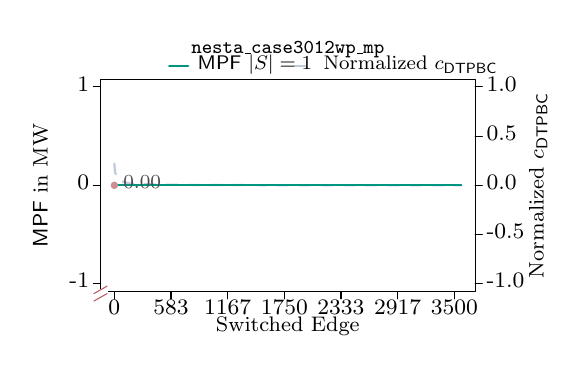
\begin{tikzpicture}[x=1pt,y=1pt]
\definecolor{fillColor}{RGB}{255,255,255}
\path[use as bounding box,fill=fillColor,fill opacity=0.00] (0,0) rectangle (440.85,271.01);
\begin{scope}
\path[clip] (  0.00,  0.00) rectangle (440.85,271.01);
\definecolor{drawColor}{RGB}{193,202,220}

\path[draw=drawColor,line width= 0.8pt,dash pattern=on 4pt off 4pt ,line join=round,line cap=round] ( 72.86,156.87) --
	( 72.94,154.71) --
	( 73.02,154.05) --
	( 73.11,153.32) --
	( 73.19,152.93) --
	( 73.27,151.12) --
	( 73.35,151.07) --
	( 73.43,149.80) --
	( 73.51,149.55) --
	( 73.60,148.69) --
	( 73.68,148.59) --
	( 73.76,148.34) --
	( 73.84,148.33) --
	( 73.92,148.30) --
	( 74.00,148.26) --
	( 74.09,148.25) --
	( 74.17,147.92) --
	( 74.25,147.84) --
	( 74.33,147.73) --
	( 74.41,147.71) --
	( 74.49,147.54) --
	( 74.58,147.50) --
	( 74.66,147.42) --
	( 74.74,147.10) --
	( 74.82,147.04) --
	( 74.90,147.03) --
	( 74.98,146.95) --
	( 75.07,146.78) --
	( 75.15,146.59) --
	( 75.23,146.38) --
	( 75.31,146.23) --
	( 75.39,146.14) --
	( 75.47,146.10) --
	( 75.56,146.07) --
	( 75.64,145.91) --
	( 75.72,145.89) --
	( 75.80,145.89) --
	( 75.88,145.85) --
	( 75.96,145.84) --
	( 76.04,145.83) --
	( 76.13,145.81) --
	( 76.21,145.80) --
	( 76.29,145.77) --
	( 76.37,145.73) --
	( 76.45,145.42) --
	( 76.53,145.27) --
	( 76.62,145.25) --
	( 76.70,145.20) --
	( 76.78,145.08) --
	( 76.86,144.76) --
	( 76.94,144.43) --
	( 77.02,144.40) --
	( 77.11,144.24) --
	( 77.19,144.07) --
	( 77.27,143.90) --
	( 77.35,143.88) --
	( 77.43,143.87) --
	( 77.51,143.74) --
	( 77.60,143.66) --
	( 77.68,143.55) --
	( 77.76,143.51) --
	( 77.84,143.48) --
	( 77.92,143.46) --
	( 78.00,143.43) --
	( 78.09,143.38) --
	( 78.17,143.32) --
	( 78.25,143.31) --
	( 78.33,143.29) --
	( 78.41,143.26) --
	( 78.49,142.92) --
	( 78.58,142.88) --
	( 78.66,142.87) --
	( 78.74,142.80) --
	( 78.82,142.72) --
	( 78.90,142.56) --
	( 78.98,142.48) --
	( 79.07,142.23) --
	( 79.15,142.09) --
	( 79.23,142.08) --
	( 79.31,142.07) --
	( 79.39,141.94) --
	( 79.47,141.92) --
	( 79.56,141.90) --
	( 79.64,141.87) --
	( 79.72,141.85) --
	( 79.80,141.81) --
	( 79.88,141.76) --
	( 79.96,141.72) --
	( 80.05,141.70) --
	( 80.13,141.70) --
	( 80.21,141.59) --
	( 80.29,141.47) --
	( 80.37,141.45) --
	( 80.45,141.44) --
	( 80.53,141.35) --
	( 80.62,141.27) --
	( 80.70,141.23) --
	( 80.78,141.23) --
	( 80.86,141.19) --
	( 80.94,141.19) --
	( 81.02,141.17) --
	( 81.11,141.15) --
	( 81.19,141.14) --
	( 81.27,141.10) --
	( 81.35,141.08) --
	( 81.43,141.06) --
	( 81.51,141.04) --
	( 81.60,141.01) --
	( 81.68,141.00) --
	( 81.76,140.99) --
	( 81.84,140.98) --
	( 81.92,140.98) --
	( 82.00,140.97) --
	( 82.09,140.96) --
	( 82.17,140.96) --
	( 82.25,140.95) --
	( 82.33,140.90) --
	( 82.41,140.89) --
	( 82.49,140.89) --
	( 82.58,140.87) --
	( 82.66,140.85) --
	( 82.74,140.84) --
	( 82.82,140.84) --
	( 82.90,140.80) --
	( 82.98,140.77) --
	( 83.07,140.77) --
	( 83.15,140.76) --
	( 83.23,140.69) --
	( 83.31,140.65) --
	( 83.39,140.64) --
	( 83.47,140.60) --
	( 83.56,140.59) --
	( 83.64,140.58) --
	( 83.72,140.58) --
	( 83.80,140.57) --
	( 83.88,140.57) --
	( 83.96,140.54) --
	( 84.05,140.53) --
	( 84.13,140.47) --
	( 84.21,140.46) --
	( 84.29,140.46) --
	( 84.37,140.42) --
	( 84.45,140.39) --
	( 84.54,140.38) --
	( 84.62,140.36) --
	( 84.70,140.35) --
	( 84.78,140.35) --
	( 84.86,140.34) --
	( 84.94,140.30) --
	( 85.02,140.26) --
	( 85.11,140.25) --
	( 85.19,140.24) --
	( 85.27,140.19) --
	( 85.35,140.19) --
	( 85.43,140.18) --
	( 85.51,140.16) --
	( 85.60,140.15) --
	( 85.68,140.14) --
	( 85.76,140.14) --
	( 85.84,140.13) --
	( 85.92,140.13) --
	( 86.00,140.12) --
	( 86.09,140.10) --
	( 86.17,140.08) --
	( 86.25,140.06) --
	( 86.33,140.04) --
	( 86.41,140.04) --
	( 86.49,140.03) --
	( 86.58,140.01) --
	( 86.66,140.01) --
	( 86.74,139.99) --
	( 86.82,139.99) --
	( 86.90,139.99) --
	( 86.98,139.98) --
	( 87.07,139.97) --
	( 87.15,139.96) --
	( 87.23,139.96) --
	( 87.31,139.96) --
	( 87.39,139.95) --
	( 87.47,139.95) --
	( 87.56,139.94) --
	( 87.64,139.94) --
	( 87.72,139.94) --
	( 87.80,139.94) --
	( 87.88,139.93) --
	( 87.96,139.92) --
	( 88.05,139.91) --
	( 88.13,139.91) --
	( 88.21,139.90) --
	( 88.29,139.90) --
	( 88.37,139.89) --
	( 88.45,139.89) --
	( 88.54,139.89) --
	( 88.62,139.89) --
	( 88.70,139.89) --
	( 88.78,139.88) --
	( 88.86,139.88) --
	( 88.94,139.86) --
	( 89.03,139.86) --
	( 89.11,139.86) --
	( 89.19,139.86) --
	( 89.27,139.85) --
	( 89.35,139.84) --
	( 89.43,139.84) --
	( 89.51,139.84) --
	( 89.60,139.82) --
	( 89.68,139.82) --
	( 89.76,139.82) --
	( 89.84,139.80) --
	( 89.92,139.80) --
	( 90.00,139.80) --
	( 90.09,139.80) --
	( 90.17,139.80) --
	( 90.25,139.79) --
	( 90.33,139.79) --
	( 90.41,139.79) --
	( 90.49,139.79) --
	( 90.58,139.78) --
	( 90.66,139.78) --
	( 90.74,139.78) --
	( 90.82,139.77) --
	( 90.90,139.76) --
	( 90.98,139.76) --
	( 91.07,139.76) --
	( 91.15,139.73) --
	( 91.23,139.73) --
	( 91.31,139.72) --
	( 91.39,139.72) --
	( 91.47,139.72) --
	( 91.56,139.71) --
	( 91.64,139.71) --
	( 91.72,139.70) --
	( 91.80,139.70) --
	( 91.88,139.70) --
	( 91.96,139.69) --
	( 92.05,139.69) --
	( 92.13,139.68) --
	( 92.21,139.68) --
	( 92.29,139.67) --
	( 92.37,139.67) --
	( 92.45,139.67) --
	( 92.54,139.67) --
	( 92.62,139.67) --
	( 92.70,139.67) --
	( 92.78,139.66) --
	( 92.86,139.66) --
	( 92.94,139.66) --
	( 93.03,139.66) --
	( 93.11,139.66) --
	( 93.19,139.65) --
	( 93.27,139.65) --
	( 93.35,139.65) --
	( 93.43,139.64) --
	( 93.52,139.64) --
	( 93.60,139.64) --
	( 93.68,139.64) --
	( 93.76,139.63) --
	( 93.84,139.63) --
	( 93.92,139.63) --
	( 94.00,139.62) --
	( 94.09,139.62) --
	( 94.17,139.62) --
	( 94.25,139.61) --
	( 94.33,139.61) --
	( 94.41,139.61) --
	( 94.49,139.61) --
	( 94.58,139.61) --
	( 94.66,139.60) --
	( 94.74,139.60) --
	( 94.82,139.60) --
	( 94.90,139.60) --
	( 94.98,139.60) --
	( 95.07,139.60) --
	( 95.15,139.59) --
	( 95.23,139.59) --
	( 95.31,139.59) --
	( 95.39,139.58) --
	( 95.47,139.58) --
	( 95.56,139.57) --
	( 95.64,139.57) --
	( 95.72,139.57) --
	( 95.80,139.57) --
	( 95.88,139.57) --
	( 95.96,139.56) --
	( 96.05,139.56) --
	( 96.13,139.56) --
	( 96.21,139.56) --
	( 96.29,139.55) --
	( 96.37,139.55) --
	( 96.45,139.55) --
	( 96.54,139.54) --
	( 96.62,139.54) --
	( 96.70,139.54) --
	( 96.78,139.54) --
	( 96.86,139.53) --
	( 96.94,139.53) --
	( 97.03,139.53) --
	( 97.11,139.53) --
	( 97.19,139.53) --
	( 97.27,139.53) --
	( 97.35,139.53) --
	( 97.43,139.52) --
	( 97.52,139.52) --
	( 97.60,139.52) --
	( 97.68,139.52) --
	( 97.76,139.51) --
	( 97.84,139.50) --
	( 97.92,139.50) --
	( 98.01,139.50) --
	( 98.09,139.50) --
	( 98.17,139.50) --
	( 98.25,139.49) --
	( 98.33,139.48) --
	( 98.41,139.48) --
	( 98.49,139.48) --
	( 98.58,139.47) --
	( 98.66,139.47) --
	( 98.74,139.47) --
	( 98.82,139.46) --
	( 98.90,139.46) --
	( 98.98,139.45) --
	( 99.07,139.45) --
	( 99.15,139.45) --
	( 99.23,139.44) --
	( 99.31,139.44) --
	( 99.39,139.44) --
	( 99.47,139.44) --
	( 99.56,139.44) --
	( 99.64,139.43) --
	( 99.72,139.43) --
	( 99.80,139.43) --
	( 99.88,139.43) --
	( 99.96,139.42) --
	(100.05,139.42) --
	(100.13,139.42) --
	(100.21,139.42) --
	(100.29,139.42) --
	(100.37,139.41) --
	(100.45,139.41) --
	(100.54,139.41) --
	(100.62,139.41) --
	(100.70,139.40) --
	(100.78,139.40) --
	(100.86,139.40) --
	(100.94,139.40) --
	(101.03,139.39) --
	(101.11,139.39) --
	(101.19,139.39) --
	(101.27,139.38) --
	(101.35,139.38) --
	(101.43,139.38) --
	(101.52,139.38) --
	(101.60,139.38) --
	(101.68,139.37) --
	(101.76,139.37) --
	(101.84,139.37) --
	(101.92,139.37) --
	(102.01,139.37) --
	(102.09,139.36) --
	(102.17,139.36) --
	(102.25,139.36) --
	(102.33,139.36) --
	(102.41,139.36) --
	(102.50,139.36) --
	(102.58,139.35) --
	(102.66,139.35) --
	(102.74,139.35) --
	(102.82,139.35) --
	(102.90,139.35) --
	(102.98,139.35) --
	(103.07,139.34) --
	(103.15,139.34) --
	(103.23,139.34) --
	(103.31,139.34) --
	(103.39,139.34) --
	(103.47,139.33) --
	(103.56,139.33) --
	(103.64,139.33) --
	(103.72,139.33) --
	(103.80,139.33) --
	(103.88,139.33) --
	(103.96,139.33) --
	(104.05,139.33) --
	(104.13,139.33) --
	(104.21,139.33) --
	(104.29,139.32) --
	(104.37,139.32) --
	(104.45,139.31) --
	(104.54,139.31) --
	(104.62,139.31) --
	(104.70,139.31) --
	(104.78,139.30) --
	(104.86,139.30) --
	(104.94,139.30) --
	(105.03,139.29) --
	(105.11,139.29) --
	(105.19,139.29) --
	(105.27,139.28) --
	(105.35,139.28) --
	(105.43,139.27) --
	(105.52,139.27) --
	(105.60,139.27) --
	(105.68,139.27) --
	(105.76,139.27) --
	(105.84,139.27) --
	(105.92,139.27) --
	(106.01,139.27) --
	(106.09,139.26) --
	(106.17,139.26) --
	(106.25,139.26) --
	(106.33,139.26) --
	(106.41,139.25) --
	(106.50,139.25) --
	(106.58,139.24) --
	(106.66,139.24) --
	(106.74,139.24) --
	(106.82,139.24) --
	(106.90,139.24) --
	(106.99,139.23) --
	(107.07,139.23) --
	(107.15,139.22) --
	(107.23,139.22) --
	(107.31,139.22) --
	(107.39,139.22) --
	(107.48,139.22) --
	(107.56,139.22) --
	(107.64,139.22) --
	(107.72,139.22) --
	(107.80,139.21) --
	(107.88,139.21) --
	(107.96,139.21) --
	(108.05,139.21) --
	(108.13,139.21) --
	(108.21,139.20) --
	(108.29,139.20) --
	(108.37,139.20) --
	(108.45,139.20) --
	(108.54,139.20) --
	(108.62,139.20) --
	(108.70,139.20) --
	(108.78,139.19) --
	(108.86,139.19) --
	(108.94,139.19) --
	(109.03,139.19) --
	(109.11,139.19) --
	(109.19,139.19) --
	(109.27,139.19) --
	(109.35,139.19) --
	(109.43,139.19) --
	(109.52,139.19) --
	(109.60,139.19) --
	(109.68,139.19) --
	(109.76,139.18) --
	(109.84,139.18) --
	(109.92,139.18) --
	(110.01,139.18) --
	(110.09,139.18) --
	(110.17,139.18) --
	(110.25,139.18) --
	(110.33,139.17) --
	(110.41,139.17) --
	(110.50,139.17) --
	(110.58,139.17) --
	(110.66,139.17) --
	(110.74,139.17) --
	(110.82,139.17) --
	(110.90,139.17) --
	(110.99,139.17) --
	(111.07,139.16) --
	(111.15,139.16) --
	(111.23,139.16) --
	(111.31,139.16) --
	(111.39,139.15) --
	(111.48,139.15) --
	(111.56,139.15) --
	(111.64,139.15) --
	(111.72,139.15) --
	(111.80,139.15) --
	(111.88,139.15) --
	(111.97,139.14) --
	(112.05,139.14) --
	(112.13,139.14) --
	(112.21,139.14) --
	(112.29,139.14) --
	(112.37,139.14) --
	(112.45,139.14) --
	(112.54,139.13) --
	(112.62,139.13) --
	(112.70,139.13) --
	(112.78,139.13) --
	(112.86,139.13) --
	(112.94,139.13) --
	(113.03,139.13) --
	(113.11,139.13) --
	(113.19,139.12) --
	(113.27,139.12) --
	(113.35,139.12) --
	(113.43,139.12) --
	(113.52,139.12) --
	(113.60,139.12) --
	(113.68,139.12) --
	(113.76,139.12) --
	(113.84,139.11) --
	(113.92,139.11) --
	(114.01,139.11) --
	(114.09,139.11) --
	(114.17,139.11) --
	(114.25,139.11) --
	(114.33,139.11) --
	(114.41,139.11) --
	(114.50,139.11) --
	(114.58,139.11) --
	(114.66,139.11) --
	(114.74,139.10) --
	(114.82,139.10) --
	(114.90,139.10) --
	(114.99,139.10) --
	(115.07,139.10) --
	(115.15,139.10) --
	(115.23,139.10) --
	(115.31,139.10) --
	(115.39,139.10) --
	(115.48,139.09) --
	(115.56,139.09) --
	(115.64,139.09) --
	(115.72,139.09) --
	(115.80,139.09) --
	(115.88,139.09) --
	(115.97,139.09) --
	(116.05,139.09) --
	(116.13,139.09) --
	(116.21,139.09) --
	(116.29,139.09) --
	(116.37,139.08) --
	(116.46,139.08) --
	(116.54,139.08) --
	(116.62,139.08) --
	(116.70,139.08) --
	(116.78,139.08) --
	(116.86,139.08) --
	(116.94,139.07) --
	(117.03,139.07) --
	(117.11,139.07) --
	(117.19,139.07) --
	(117.27,139.07) --
	(117.35,139.06) --
	(117.43,139.06) --
	(117.52,139.06) --
	(117.60,139.06) --
	(117.68,139.06) --
	(117.76,139.06) --
	(117.84,139.06) --
	(117.92,139.06) --
	(118.01,139.06) --
	(118.09,139.05) --
	(118.17,139.05) --
	(118.25,139.05) --
	(118.33,139.05) --
	(118.41,139.05) --
	(118.50,139.05) --
	(118.58,139.05) --
	(118.66,139.05) --
	(118.74,139.05) --
	(118.82,139.04) --
	(118.90,139.04) --
	(118.99,139.04) --
	(119.07,139.04) --
	(119.15,139.04) --
	(119.23,139.04) --
	(119.31,139.04) --
	(119.39,139.04) --
	(119.48,139.03) --
	(119.56,139.03) --
	(119.64,139.03) --
	(119.72,139.03) --
	(119.80,139.03) --
	(119.88,139.03) --
	(119.97,139.03) --
	(120.05,139.03) --
	(120.13,139.03) --
	(120.21,139.03) --
	(120.29,139.03) --
	(120.37,139.03) --
	(120.46,139.02) --
	(120.54,139.02) --
	(120.62,139.02) --
	(120.70,139.02) --
	(120.78,139.02) --
	(120.86,139.02) --
	(120.95,139.02) --
	(121.03,139.02) --
	(121.11,139.01) --
	(121.19,139.01) --
	(121.27,139.01) --
	(121.35,139.01) --
	(121.43,139.01) --
	(121.52,139.01) --
	(121.60,139.01) --
	(121.68,139.01) --
	(121.76,139.01) --
	(121.84,139.01) --
	(121.92,139.01) --
	(122.01,139.00) --
	(122.09,139.00) --
	(122.17,139.00) --
	(122.25,139.00) --
	(122.33,139.00) --
	(122.41,139.00) --
	(122.50,139.00) --
	(122.58,139.00) --
	(122.66,139.00) --
	(122.74,139.00) --
	(122.82,139.00) --
	(122.90,139.00) --
	(122.99,139.00) --
	(123.07,139.00) --
	(123.15,139.00) --
	(123.23,139.00) --
	(123.31,139.00) --
	(123.39,139.00) --
	(123.48,139.00) --
	(123.56,138.99) --
	(123.64,138.99) --
	(123.72,138.99) --
	(123.80,138.99) --
	(123.88,138.99) --
	(123.97,138.99) --
	(124.05,138.99) --
	(124.13,138.99) --
	(124.21,138.99) --
	(124.29,138.99) --
	(124.37,138.99) --
	(124.46,138.99) --
	(124.54,138.99) --
	(124.62,138.99) --
	(124.70,138.99) --
	(124.78,138.99) --
	(124.86,138.99) --
	(124.95,138.99) --
	(125.03,138.98) --
	(125.11,138.98) --
	(125.19,138.98) --
	(125.27,138.98) --
	(125.35,138.98) --
	(125.44,138.98) --
	(125.52,138.98) --
	(125.60,138.98) --
	(125.68,138.98) --
	(125.76,138.98) --
	(125.84,138.98) --
	(125.92,138.98) --
	(126.01,138.98) --
	(126.09,138.98) --
	(126.17,138.98) --
	(126.25,138.98) --
	(126.33,138.98) --
	(126.41,138.97) --
	(126.50,138.97) --
	(126.58,138.97) --
	(126.66,138.97) --
	(126.74,138.97) --
	(126.82,138.97) --
	(126.90,138.97) --
	(126.99,138.97) --
	(127.07,138.97) --
	(127.15,138.97) --
	(127.23,138.97) --
	(127.31,138.97) --
	(127.39,138.96) --
	(127.48,138.96) --
	(127.56,138.96) --
	(127.64,138.96) --
	(127.72,138.96) --
	(127.80,138.96) --
	(127.88,138.96) --
	(127.97,138.96) --
	(128.05,138.96) --
	(128.13,138.96) --
	(128.21,138.96) --
	(128.29,138.96) --
	(128.37,138.95) --
	(128.46,138.95) --
	(128.54,138.95) --
	(128.62,138.95) --
	(128.70,138.95) --
	(128.78,138.95) --
	(128.86,138.95) --
	(128.95,138.95) --
	(129.03,138.95) --
	(129.11,138.95) --
	(129.19,138.95) --
	(129.27,138.95) --
	(129.35,138.95) --
	(129.44,138.95) --
	(129.52,138.95) --
	(129.60,138.95) --
	(129.68,138.95) --
	(129.76,138.94) --
	(129.84,138.94) --
	(129.93,138.94) --
	(130.01,138.94) --
	(130.09,138.94) --
	(130.17,138.94) --
	(130.25,138.94) --
	(130.33,138.94) --
	(130.41,138.94) --
	(130.50,138.94) --
	(130.58,138.93) --
	(130.66,138.93) --
	(130.74,138.93) --
	(130.82,138.93) --
	(130.90,138.93) --
	(130.99,138.93) --
	(131.07,138.93) --
	(131.15,138.93) --
	(131.23,138.93) --
	(131.31,138.93) --
	(131.39,138.93) --
	(131.48,138.93) --
	(131.56,138.93) --
	(131.64,138.93) --
	(131.72,138.93) --
	(131.80,138.93) --
	(131.88,138.92) --
	(131.97,138.92) --
	(132.05,138.92) --
	(132.13,138.92) --
	(132.21,138.92) --
	(132.29,138.92) --
	(132.37,138.92) --
	(132.46,138.92) --
	(132.54,138.92) --
	(132.62,138.92) --
	(132.70,138.92) --
	(132.78,138.92) --
	(132.86,138.92) --
	(132.95,138.92) --
	(133.03,138.92) --
	(133.11,138.92) --
	(133.19,138.91) --
	(133.27,138.91) --
	(133.35,138.91) --
	(133.44,138.91) --
	(133.52,138.91) --
	(133.60,138.91) --
	(133.68,138.91) --
	(133.76,138.91) --
	(133.84,138.91) --
	(133.93,138.91) --
	(134.01,138.90) --
	(134.09,138.90) --
	(134.17,138.90) --
	(134.25,138.90) --
	(134.33,138.90) --
	(134.42,138.90) --
	(134.50,138.90) --
	(134.58,138.90) --
	(134.66,138.90) --
	(134.74,138.90) --
	(134.82,138.90) --
	(134.90,138.90) --
	(134.99,138.90) --
	(135.07,138.90) --
	(135.15,138.90) --
	(135.23,138.90) --
	(135.31,138.90) --
	(135.39,138.90) --
	(135.48,138.90) --
	(135.56,138.89) --
	(135.64,138.89) --
	(135.72,138.89) --
	(135.80,138.89) --
	(135.88,138.89) --
	(135.97,138.89) --
	(136.05,138.89) --
	(136.13,138.89) --
	(136.21,138.89) --
	(136.29,138.89) --
	(136.37,138.89) --
	(136.46,138.89) --
	(136.54,138.88) --
	(136.62,138.88) --
	(136.70,138.88) --
	(136.78,138.88) --
	(136.86,138.88) --
	(136.95,138.88) --
	(137.03,138.88) --
	(137.11,138.88) --
	(137.19,138.88) --
	(137.27,138.88) --
	(137.35,138.88) --
	(137.44,138.88) --
	(137.52,138.88) --
	(137.60,138.88) --
	(137.68,138.88) --
	(137.76,138.88) --
	(137.84,138.88) --
	(137.93,138.88) --
	(138.01,138.88) --
	(138.09,138.88) --
	(138.17,138.88) --
	(138.25,138.88) --
	(138.33,138.88) --
	(138.42,138.88) --
	(138.50,138.88) --
	(138.58,138.88) --
	(138.66,138.88) --
	(138.74,138.88) --
	(138.82,138.87) --
	(138.91,138.87) --
	(138.99,138.87) --
	(139.07,138.87) --
	(139.15,138.87) --
	(139.23,138.87) --
	(139.31,138.87) --
	(139.39,138.87) --
	(139.48,138.87) --
	(139.56,138.87) --
	(139.64,138.87) --
	(139.72,138.87) --
	(139.80,138.87) --
	(139.88,138.87) --
	(139.97,138.87) --
	(140.05,138.87) --
	(140.13,138.87) --
	(140.21,138.87) --
	(140.29,138.87) --
	(140.37,138.87) --
	(140.46,138.87) --
	(140.54,138.87) --
	(140.62,138.86) --
	(140.70,138.86) --
	(140.78,138.86) --
	(140.86,138.86) --
	(140.95,138.86) --
	(141.03,138.86) --
	(141.11,138.86) --
	(141.19,138.86) --
	(141.27,138.86) --
	(141.35,138.86) --
	(141.44,138.86) --
	(141.52,138.86) --
	(141.60,138.86) --
	(141.68,138.86) --
	(141.76,138.86) --
	(141.84,138.86) --
	(141.93,138.86) --
	(142.01,138.86) --
	(142.09,138.86) --
	(142.17,138.86) --
	(142.25,138.85) --
	(142.33,138.85) --
	(142.42,138.85) --
	(142.50,138.85) --
	(142.58,138.85) --
	(142.66,138.85) --
	(142.74,138.85) --
	(142.82,138.85) --
	(142.91,138.85) --
	(142.99,138.85) --
	(143.07,138.85) --
	(143.15,138.85) --
	(143.23,138.85) --
	(143.31,138.84) --
	(143.40,138.84) --
	(143.48,138.84) --
	(143.56,138.84) --
	(143.64,138.84) --
	(143.72,138.84) --
	(143.80,138.84) --
	(143.89,138.84) --
	(143.97,138.84) --
	(144.05,138.84) --
	(144.13,138.84) --
	(144.21,138.84) --
	(144.29,138.84) --
	(144.37,138.84) --
	(144.46,138.84) --
	(144.54,138.84) --
	(144.62,138.84) --
	(144.70,138.84) --
	(144.78,138.84) --
	(144.86,138.84) --
	(144.95,138.84) --
	(145.03,138.84) --
	(145.11,138.84) --
	(145.19,138.83) --
	(145.27,138.83) --
	(145.35,138.83) --
	(145.44,138.83) --
	(145.52,138.83) --
	(145.60,138.83) --
	(145.68,138.83) --
	(145.76,138.83) --
	(145.84,138.83) --
	(145.93,138.83) --
	(146.01,138.83) --
	(146.09,138.83) --
	(146.17,138.83) --
	(146.25,138.83) --
	(146.33,138.83) --
	(146.42,138.83) --
	(146.50,138.83) --
	(146.58,138.83) --
	(146.66,138.83) --
	(146.74,138.83) --
	(146.82,138.83) --
	(146.91,138.83) --
	(146.99,138.83) --
	(147.07,138.83) --
	(147.15,138.83) --
	(147.23,138.83) --
	(147.31,138.83) --
	(147.40,138.82) --
	(147.48,138.82) --
	(147.56,138.82) --
	(147.64,138.82) --
	(147.72,138.82) --
	(147.80,138.82) --
	(147.89,138.82) --
	(147.97,138.82) --
	(148.05,138.82) --
	(148.13,138.82) --
	(148.21,138.82) --
	(148.29,138.82) --
	(148.38,138.82) --
	(148.46,138.82) --
	(148.54,138.82) --
	(148.62,138.82) --
	(148.70,138.82) --
	(148.78,138.82) --
	(148.86,138.82) --
	(148.95,138.82) --
	(149.03,138.82) --
	(149.11,138.82) --
	(149.19,138.82) --
	(149.27,138.82) --
	(149.35,138.82) --
	(149.44,138.82) --
	(149.52,138.82) --
	(149.60,138.82) --
	(149.68,138.82) --
	(149.76,138.82) --
	(149.84,138.82) --
	(149.93,138.82) --
	(150.01,138.82) --
	(150.09,138.81) --
	(150.17,138.81) --
	(150.25,138.81) --
	(150.33,138.81) --
	(150.42,138.81) --
	(150.50,138.81) --
	(150.58,138.81) --
	(150.66,138.81) --
	(150.74,138.81) --
	(150.82,138.81) --
	(150.91,138.81) --
	(150.99,138.81) --
	(151.07,138.81) --
	(151.15,138.81) --
	(151.23,138.81) --
	(151.31,138.81) --
	(151.40,138.81) --
	(151.48,138.81) --
	(151.56,138.81) --
	(151.64,138.81) --
	(151.72,138.81) --
	(151.80,138.80) --
	(151.89,138.80) --
	(151.97,138.80) --
	(152.05,138.80) --
	(152.13,138.80) --
	(152.21,138.80) --
	(152.29,138.80) --
	(152.38,138.80) --
	(152.46,138.80) --
	(152.54,138.80) --
	(152.62,138.80) --
	(152.70,138.80) --
	(152.78,138.80) --
	(152.87,138.80) --
	(152.95,138.80) --
	(153.03,138.80) --
	(153.11,138.80) --
	(153.19,138.80) --
	(153.27,138.80) --
	(153.35,138.80) --
	(153.44,138.80) --
	(153.52,138.80) --
	(153.60,138.80) --
	(153.68,138.80) --
	(153.76,138.80) --
	(153.84,138.80) --
	(153.93,138.80) --
	(154.01,138.80) --
	(154.09,138.80) --
	(154.17,138.80) --
	(154.25,138.79) --
	(154.33,138.79) --
	(154.42,138.79) --
	(154.50,138.79) --
	(154.58,138.79) --
	(154.66,138.79) --
	(154.74,138.79) --
	(154.82,138.79) --
	(154.91,138.79) --
	(154.99,138.79) --
	(155.07,138.79) --
	(155.15,138.79) --
	(155.23,138.79) --
	(155.31,138.79) --
	(155.40,138.79) --
	(155.48,138.79) --
	(155.56,138.79) --
	(155.64,138.79) --
	(155.72,138.79) --
	(155.80,138.79) --
	(155.89,138.79) --
	(155.97,138.79) --
	(156.05,138.79) --
	(156.13,138.79) --
	(156.21,138.79) --
	(156.29,138.79) --
	(156.38,138.79) --
	(156.46,138.79) --
	(156.54,138.79) --
	(156.62,138.79) --
	(156.70,138.79) --
	(156.78,138.78) --
	(156.87,138.78) --
	(156.95,138.78) --
	(157.03,138.78) --
	(157.11,138.78) --
	(157.19,138.78) --
	(157.27,138.78) --
	(157.36,138.78) --
	(157.44,138.78) --
	(157.52,138.78) --
	(157.60,138.78) --
	(157.68,138.78) --
	(157.76,138.78) --
	(157.84,138.78) --
	(157.93,138.78) --
	(158.01,138.78) --
	(158.09,138.78) --
	(158.17,138.78) --
	(158.25,138.78) --
	(158.33,138.78) --
	(158.42,138.78) --
	(158.50,138.78) --
	(158.58,138.78) --
	(158.66,138.78) --
	(158.74,138.78) --
	(158.82,138.78) --
	(158.91,138.77) --
	(158.99,138.77) --
	(159.07,138.77) --
	(159.15,138.77) --
	(159.23,138.77) --
	(159.31,138.77) --
	(159.40,138.77) --
	(159.48,138.77) --
	(159.56,138.77) --
	(159.64,138.77) --
	(159.72,138.77) --
	(159.80,138.77) --
	(159.89,138.77) --
	(159.97,138.77) --
	(160.05,138.77) --
	(160.13,138.77) --
	(160.21,138.77) --
	(160.29,138.77) --
	(160.38,138.77) --
	(160.46,138.77) --
	(160.54,138.77) --
	(160.62,138.77) --
	(160.70,138.77) --
	(160.78,138.77) --
	(160.87,138.77) --
	(160.95,138.77) --
	(161.03,138.77) --
	(161.11,138.77) --
	(161.19,138.77) --
	(161.27,138.77) --
	(161.36,138.77) --
	(161.44,138.77) --
	(161.52,138.77) --
	(161.60,138.77) --
	(161.68,138.77) --
	(161.76,138.77) --
	(161.85,138.77) --
	(161.93,138.77) --
	(162.01,138.77) --
	(162.09,138.77) --
	(162.17,138.77) --
	(162.25,138.77) --
	(162.33,138.77) --
	(162.42,138.76) --
	(162.50,138.76) --
	(162.58,138.76) --
	(162.66,138.76) --
	(162.74,138.76) --
	(162.82,138.76) --
	(162.91,138.76) --
	(162.99,138.76) --
	(163.07,138.76) --
	(163.15,138.76) --
	(163.23,138.76) --
	(163.31,138.76) --
	(163.40,138.76) --
	(163.48,138.76) --
	(163.56,138.76) --
	(163.64,138.76) --
	(163.72,138.76) --
	(163.80,138.76) --
	(163.89,138.76) --
	(163.97,138.76) --
	(164.05,138.76) --
	(164.13,138.76) --
	(164.21,138.76) --
	(164.29,138.76) --
	(164.38,138.76) --
	(164.46,138.76) --
	(164.54,138.76) --
	(164.62,138.76) --
	(164.70,138.76) --
	(164.78,138.76) --
	(164.87,138.76) --
	(164.95,138.76) --
	(165.03,138.75) --
	(165.11,138.75) --
	(165.19,138.75) --
	(165.27,138.75) --
	(165.36,138.75) --
	(165.44,138.75) --
	(165.52,138.75) --
	(165.60,138.75) --
	(165.68,138.75) --
	(165.76,138.75) --
	(165.85,138.75) --
	(165.93,138.75) --
	(166.01,138.75) --
	(166.09,138.75) --
	(166.17,138.75) --
	(166.25,138.75) --
	(166.34,138.75) --
	(166.42,138.75) --
	(166.50,138.75) --
	(166.58,138.75) --
	(166.66,138.75) --
	(166.74,138.75) --
	(166.82,138.75) --
	(166.91,138.75) --
	(166.99,138.75) --
	(167.07,138.75) --
	(167.15,138.75) --
	(167.23,138.75) --
	(167.31,138.75) --
	(167.40,138.75) --
	(167.48,138.74) --
	(167.56,138.74) --
	(167.64,138.74) --
	(167.72,138.74) --
	(167.80,138.74) --
	(167.89,138.74) --
	(167.97,138.74) --
	(168.05,138.74) --
	(168.13,138.74) --
	(168.21,138.74) --
	(168.29,138.74) --
	(168.38,138.74) --
	(168.46,138.74) --
	(168.54,138.74) --
	(168.62,138.74) --
	(168.70,138.74) --
	(168.78,138.74) --
	(168.87,138.74) --
	(168.95,138.74) --
	(169.03,138.74) --
	(169.11,138.74) --
	(169.19,138.74) --
	(169.27,138.74) --
	(169.36,138.74) --
	(169.44,138.74) --
	(169.52,138.74) --
	(169.60,138.74) --
	(169.68,138.74) --
	(169.76,138.74) --
	(169.85,138.74) --
	(169.93,138.74) --
	(170.01,138.74) --
	(170.09,138.74) --
	(170.17,138.74) --
	(170.25,138.74) --
	(170.34,138.74) --
	(170.42,138.74) --
	(170.50,138.74) --
	(170.58,138.74) --
	(170.66,138.74) --
	(170.74,138.73) --
	(170.83,138.73) --
	(170.91,138.73) --
	(170.99,138.73) --
	(171.07,138.73) --
	(171.15,138.73) --
	(171.23,138.73) --
	(171.31,138.73) --
	(171.40,138.73) --
	(171.48,138.73) --
	(171.56,138.73) --
	(171.64,138.73) --
	(171.72,138.73) --
	(171.80,138.73) --
	(171.89,138.73) --
	(171.97,138.73) --
	(172.05,138.73) --
	(172.13,138.73) --
	(172.21,138.73) --
	(172.29,138.73) --
	(172.38,138.73) --
	(172.46,138.73) --
	(172.54,138.73) --
	(172.62,138.73) --
	(172.70,138.73) --
	(172.78,138.73) --
	(172.87,138.73) --
	(172.95,138.73) --
	(173.03,138.73) --
	(173.11,138.73) --
	(173.19,138.73) --
	(173.27,138.73) --
	(173.36,138.73) --
	(173.44,138.73) --
	(173.52,138.72) --
	(173.60,138.72) --
	(173.68,138.72) --
	(173.76,138.72) --
	(173.85,138.72) --
	(173.93,138.72) --
	(174.01,138.72) --
	(174.09,138.72) --
	(174.17,138.72) --
	(174.25,138.72) --
	(174.34,138.72) --
	(174.42,138.72) --
	(174.50,138.72) --
	(174.58,138.72) --
	(174.66,138.72) --
	(174.74,138.72) --
	(174.83,138.72) --
	(174.91,138.72) --
	(174.99,138.72) --
	(175.07,138.72) --
	(175.15,138.72) --
	(175.23,138.72) --
	(175.32,138.72) --
	(175.40,138.72) --
	(175.48,138.72) --
	(175.56,138.72) --
	(175.64,138.72) --
	(175.72,138.72) --
	(175.81,138.72) --
	(175.89,138.72) --
	(175.97,138.72) --
	(176.05,138.72) --
	(176.13,138.72) --
	(176.21,138.72) --
	(176.29,138.72) --
	(176.38,138.72) --
	(176.46,138.72) --
	(176.54,138.72) --
	(176.62,138.72) --
	(176.70,138.72) --
	(176.78,138.72) --
	(176.87,138.72) --
	(176.95,138.72) --
	(177.03,138.72) --
	(177.11,138.72) --
	(177.19,138.72) --
	(177.27,138.72) --
	(177.36,138.72) --
	(177.44,138.72) --
	(177.52,138.72) --
	(177.60,138.72) --
	(177.68,138.72) --
	(177.76,138.72) --
	(177.85,138.72) --
	(177.93,138.72) --
	(178.01,138.72) --
	(178.09,138.72) --
	(178.17,138.72) --
	(178.25,138.72) --
	(178.34,138.72) --
	(178.42,138.72) --
	(178.50,138.72) --
	(178.58,138.72) --
	(178.66,138.71) --
	(178.74,138.71) --
	(178.83,138.71) --
	(178.91,138.71) --
	(178.99,138.71) --
	(179.07,138.71) --
	(179.15,138.71) --
	(179.23,138.71) --
	(179.32,138.71) --
	(179.40,138.71) --
	(179.48,138.71) --
	(179.56,138.71) --
	(179.64,138.71) --
	(179.72,138.71) --
	(179.81,138.71) --
	(179.89,138.71) --
	(179.97,138.71) --
	(180.05,138.71) --
	(180.13,138.71) --
	(180.21,138.71) --
	(180.30,138.71) --
	(180.38,138.71) --
	(180.46,138.71) --
	(180.54,138.71) --
	(180.62,138.71) --
	(180.70,138.71) --
	(180.78,138.71) --
	(180.87,138.71) --
	(180.95,138.71) --
	(181.03,138.71) --
	(181.11,138.71) --
	(181.19,138.71) --
	(181.27,138.71) --
	(181.36,138.71) --
	(181.44,138.71) --
	(181.52,138.71) --
	(181.60,138.71) --
	(181.68,138.71) --
	(181.76,138.71) --
	(181.85,138.71) --
	(181.93,138.71) --
	(182.01,138.71) --
	(182.09,138.71) --
	(182.17,138.71) --
	(182.25,138.71) --
	(182.34,138.71) --
	(182.42,138.71) --
	(182.50,138.71) --
	(182.58,138.71) --
	(182.66,138.71) --
	(182.74,138.71) --
	(182.83,138.71) --
	(182.91,138.71) --
	(182.99,138.71) --
	(183.07,138.71) --
	(183.15,138.71) --
	(183.23,138.71) --
	(183.32,138.71) --
	(183.40,138.71) --
	(183.48,138.71) --
	(183.56,138.70) --
	(183.64,138.70) --
	(183.72,138.70) --
	(183.81,138.70) --
	(183.89,138.70) --
	(183.97,138.70) --
	(184.05,138.70) --
	(184.13,138.70) --
	(184.21,138.70) --
	(184.30,138.70) --
	(184.38,138.70) --
	(184.46,138.70) --
	(184.54,138.70) --
	(184.62,138.70) --
	(184.70,138.70) --
	(184.79,138.70) --
	(184.87,138.70) --
	(184.95,138.70) --
	(185.03,138.70) --
	(185.11,138.70) --
	(185.19,138.70) --
	(185.27,138.70) --
	(185.36,138.70) --
	(185.44,138.70) --
	(185.52,138.70) --
	(185.60,138.70) --
	(185.68,138.70) --
	(185.76,138.70) --
	(185.85,138.70) --
	(185.93,138.70) --
	(186.01,138.70) --
	(186.09,138.70) --
	(186.17,138.70) --
	(186.25,138.70) --
	(186.34,138.70) --
	(186.42,138.70) --
	(186.50,138.70) --
	(186.58,138.70) --
	(186.66,138.70) --
	(186.74,138.70) --
	(186.83,138.70) --
	(186.91,138.70) --
	(186.99,138.70) --
	(187.07,138.70) --
	(187.15,138.70) --
	(187.23,138.70) --
	(187.32,138.70) --
	(187.40,138.70) --
	(187.48,138.69) --
	(187.56,138.69) --
	(187.64,138.69) --
	(187.72,138.69) --
	(187.81,138.69) --
	(187.89,138.69) --
	(187.97,138.69) --
	(188.05,138.69) --
	(188.13,138.69) --
	(188.21,138.69) --
	(188.30,138.69) --
	(188.38,138.69) --
	(188.46,138.69) --
	(188.54,138.69) --
	(188.62,138.69) --
	(188.70,138.69) --
	(188.79,138.69) --
	(188.87,138.69) --
	(188.95,138.69) --
	(189.03,138.69) --
	(189.11,138.69) --
	(189.19,138.69) --
	(189.28,138.69) --
	(189.36,138.69) --
	(189.44,138.69) --
	(189.52,138.69) --
	(189.60,138.69) --
	(189.68,138.69) --
	(189.76,138.69) --
	(189.85,138.69) --
	(189.93,138.69) --
	(190.01,138.69) --
	(190.09,138.69) --
	(190.17,138.69) --
	(190.25,138.69) --
	(190.34,138.69) --
	(190.42,138.69) --
	(190.50,138.69) --
	(190.58,138.69) --
	(190.66,138.69) --
	(190.74,138.69) --
	(190.83,138.69) --
	(190.91,138.69) --
	(190.99,138.69) --
	(191.07,138.68) --
	(191.15,138.68) --
	(191.23,138.68) --
	(191.32,138.68) --
	(191.40,138.68) --
	(191.48,138.68) --
	(191.56,138.68) --
	(191.64,138.68) --
	(191.72,138.68) --
	(191.81,138.68) --
	(191.89,138.68) --
	(191.97,138.68) --
	(192.05,138.68) --
	(192.13,138.68) --
	(192.21,138.68) --
	(192.30,138.68) --
	(192.38,138.68) --
	(192.46,138.68) --
	(192.54,138.68) --
	(192.62,138.68) --
	(192.70,138.68) --
	(192.79,138.68) --
	(192.87,138.68) --
	(192.95,138.68) --
	(193.03,138.68) --
	(193.11,138.68) --
	(193.19,138.68) --
	(193.28,138.68) --
	(193.36,138.68) --
	(193.44,138.68) --
	(193.52,138.68) --
	(193.60,138.68) --
	(193.68,138.68) --
	(193.77,138.68) --
	(193.85,138.68) --
	(193.93,138.68) --
	(194.01,138.68) --
	(194.09,138.68) --
	(194.17,138.68) --
	(194.25,138.68) --
	(194.34,138.68) --
	(194.42,138.68) --
	(194.50,138.68) --
	(194.58,138.67) --
	(194.66,138.67) --
	(194.74,138.67) --
	(194.83,138.67) --
	(194.91,138.67) --
	(194.99,138.67) --
	(195.07,138.67) --
	(195.15,138.67) --
	(195.23,138.67) --
	(195.32,138.67) --
	(195.40,138.67) --
	(195.48,138.67) --
	(195.56,138.67) --
	(195.64,138.67) --
	(195.72,138.67) --
	(195.81,138.67) --
	(195.89,138.67) --
	(195.97,138.67) --
	(196.05,138.67) --
	(196.13,138.67) --
	(196.21,138.67) --
	(196.30,138.67) --
	(196.38,138.67) --
	(196.46,138.67) --
	(196.54,138.67) --
	(196.62,138.67) --
	(196.70,138.67) --
	(196.79,138.67) --
	(196.87,138.67) --
	(196.95,138.67) --
	(197.03,138.67) --
	(197.11,138.67) --
	(197.19,138.67) --
	(197.28,138.67) --
	(197.36,138.67) --
	(197.44,138.67) --
	(197.52,138.67) --
	(197.60,138.67) --
	(197.68,138.67) --
	(197.77,138.67) --
	(197.85,138.67) --
	(197.93,138.67) --
	(198.01,138.67) --
	(198.09,138.67) --
	(198.17,138.67) --
	(198.26,138.67) --
	(198.34,138.67) --
	(198.42,138.67) --
	(198.50,138.67) --
	(198.58,138.67) --
	(198.66,138.67) --
	(198.74,138.67) --
	(198.83,138.67) --
	(198.91,138.67) --
	(198.99,138.67) --
	(199.07,138.67) --
	(199.15,138.67) --
	(199.23,138.67) --
	(199.32,138.67) --
	(199.40,138.67) --
	(199.48,138.67) --
	(199.56,138.67) --
	(199.64,138.67) --
	(199.72,138.67) --
	(199.81,138.67) --
	(199.89,138.67) --
	(199.97,138.67) --
	(200.05,138.67) --
	(200.13,138.67) --
	(200.21,138.67) --
	(200.30,138.67) --
	(200.38,138.67) --
	(200.46,138.67) --
	(200.54,138.67) --
	(200.62,138.67) --
	(200.70,138.67) --
	(200.79,138.67) --
	(200.87,138.67) --
	(200.95,138.67) --
	(201.03,138.67) --
	(201.11,138.67) --
	(201.19,138.67) --
	(201.28,138.67) --
	(201.36,138.67) --
	(201.44,138.66) --
	(201.52,138.66) --
	(201.60,138.66) --
	(201.68,138.66) --
	(201.77,138.66) --
	(201.85,138.66) --
	(201.93,138.66) --
	(202.01,138.66) --
	(202.09,138.66) --
	(202.17,138.66) --
	(202.26,138.66) --
	(202.34,138.66) --
	(202.42,138.66) --
	(202.50,138.66) --
	(202.58,138.66) --
	(202.66,138.66) --
	(202.75,138.66) --
	(202.83,138.66) --
	(202.91,138.66) --
	(202.99,138.66) --
	(203.07,138.66) --
	(203.15,138.66) --
	(203.23,138.66) --
	(203.32,138.66) --
	(203.40,138.66) --
	(203.48,138.66) --
	(203.56,138.66) --
	(203.64,138.66) --
	(203.72,138.66) --
	(203.81,138.66) --
	(203.89,138.66) --
	(203.97,138.66) --
	(204.05,138.66) --
	(204.13,138.66) --
	(204.21,138.66) --
	(204.30,138.66) --
	(204.38,138.66) --
	(204.46,138.66) --
	(204.54,138.66) --
	(204.62,138.66) --
	(204.70,138.66) --
	(204.79,138.66) --
	(204.87,138.66) --
	(204.95,138.66) --
	(205.03,138.66) --
	(205.11,138.66) --
	(205.19,138.66) --
	(205.28,138.66) --
	(205.36,138.66) --
	(205.44,138.66) --
	(205.52,138.66) --
	(205.60,138.66) --
	(205.68,138.66) --
	(205.77,138.66) --
	(205.85,138.66) --
	(205.93,138.66) --
	(206.01,138.66) --
	(206.09,138.66) --
	(206.17,138.66) --
	(206.26,138.66) --
	(206.34,138.66) --
	(206.42,138.66) --
	(206.50,138.66) --
	(206.58,138.66) --
	(206.66,138.66) --
	(206.75,138.66) --
	(206.83,138.66) --
	(206.91,138.66) --
	(206.99,138.66) --
	(207.07,138.66) --
	(207.15,138.66) --
	(207.24,138.66) --
	(207.32,138.66) --
	(207.40,138.66) --
	(207.48,138.66) --
	(207.56,138.66) --
	(207.64,138.66) --
	(207.72,138.66) --
	(207.81,138.66) --
	(207.89,138.66) --
	(207.97,138.66) --
	(208.05,138.66) --
	(208.13,138.66) --
	(208.21,138.65) --
	(208.30,138.65) --
	(208.38,138.65) --
	(208.46,138.65) --
	(208.54,138.65) --
	(208.62,138.65) --
	(208.70,138.65) --
	(208.79,138.65) --
	(208.87,138.65) --
	(208.95,138.65) --
	(209.03,138.65) --
	(209.11,138.65) --
	(209.19,138.65) --
	(209.28,138.65) --
	(209.36,138.65) --
	(209.44,138.65) --
	(209.52,138.65) --
	(209.60,138.65) --
	(209.68,138.65) --
	(209.77,138.65) --
	(209.85,138.65) --
	(209.93,138.65) --
	(210.01,138.65) --
	(210.09,138.65) --
	(210.17,138.65) --
	(210.26,138.65) --
	(210.34,138.65) --
	(210.42,138.65) --
	(210.50,138.65) --
	(210.58,138.65) --
	(210.66,138.65) --
	(210.75,138.65) --
	(210.83,138.65) --
	(210.91,138.65) --
	(210.99,138.65) --
	(211.07,138.65) --
	(211.15,138.65) --
	(211.24,138.65) --
	(211.32,138.65) --
	(211.40,138.65) --
	(211.48,138.65) --
	(211.56,138.65) --
	(211.64,138.65) --
	(211.73,138.65) --
	(211.81,138.65) --
	(211.89,138.65) --
	(211.97,138.65) --
	(212.05,138.65) --
	(212.13,138.65) --
	(212.22,138.65) --
	(212.30,138.65) --
	(212.38,138.65) --
	(212.46,138.65) --
	(212.54,138.65) --
	(212.62,138.65) --
	(212.70,138.65) --
	(212.79,138.65) --
	(212.87,138.65) --
	(212.95,138.65) --
	(213.03,138.65) --
	(213.11,138.65) --
	(213.19,138.64) --
	(213.28,138.64) --
	(213.36,138.64) --
	(213.44,138.64) --
	(213.52,138.64) --
	(213.60,138.64) --
	(213.68,138.64) --
	(213.77,138.64) --
	(213.85,138.64) --
	(213.93,138.64) --
	(214.01,138.64) --
	(214.09,138.64) --
	(214.17,138.64) --
	(214.26,138.64) --
	(214.34,138.64) --
	(214.42,138.64) --
	(214.50,138.64) --
	(214.58,138.64) --
	(214.66,138.64) --
	(214.75,138.64) --
	(214.83,138.64) --
	(214.91,138.64) --
	(214.99,138.64) --
	(215.07,138.64) --
	(215.15,138.64) --
	(215.24,138.64) --
	(215.32,138.64) --
	(215.40,138.64) --
	(215.48,138.64) --
	(215.56,138.64) --
	(215.64,138.64) --
	(215.73,138.64) --
	(215.81,138.64) --
	(215.89,138.64) --
	(215.97,138.64) --
	(216.05,138.64) --
	(216.13,138.64) --
	(216.22,138.64) --
	(216.30,138.64) --
	(216.38,138.64) --
	(216.46,138.64) --
	(216.54,138.64) --
	(216.62,138.64) --
	(216.71,138.64) --
	(216.79,138.64) --
	(216.87,138.64) --
	(216.95,138.64) --
	(217.03,138.64) --
	(217.11,138.64) --
	(217.19,138.64) --
	(217.28,138.64) --
	(217.36,138.64) --
	(217.44,138.64) --
	(217.52,138.64) --
	(217.60,138.64) --
	(217.68,138.64) --
	(217.77,138.64) --
	(217.85,138.64) --
	(217.93,138.64) --
	(218.01,138.64) --
	(218.09,138.63) --
	(218.17,138.63) --
	(218.26,138.63) --
	(218.34,138.63) --
	(218.42,138.63) --
	(218.50,138.63) --
	(218.58,138.63) --
	(218.66,138.63) --
	(218.75,138.63) --
	(218.83,138.63) --
	(218.91,138.63) --
	(218.99,138.63) --
	(219.07,138.63) --
	(219.15,138.63) --
	(219.24,138.63) --
	(219.32,138.63) --
	(219.40,138.63) --
	(219.48,138.63) --
	(219.56,138.63) --
	(219.64,138.63) --
	(219.73,138.63) --
	(219.81,138.63) --
	(219.89,138.63) --
	(219.97,138.63) --
	(220.05,138.63) --
	(220.13,138.63) --
	(220.22,138.63) --
	(220.30,138.63) --
	(220.38,138.63) --
	(220.46,138.63) --
	(220.54,138.63) --
	(220.62,138.63) --
	(220.71,138.63) --
	(220.79,138.63) --
	(220.87,138.63) --
	(220.95,138.63) --
	(221.03,138.63) --
	(221.11,138.63) --
	(221.20,138.63) --
	(221.28,138.63) --
	(221.36,138.63) --
	(221.44,138.63) --
	(221.52,138.63) --
	(221.60,138.63) --
	(221.68,138.63) --
	(221.77,138.63) --
	(221.85,138.63) --
	(221.93,138.63) --
	(222.01,138.63) --
	(222.09,138.63) --
	(222.17,138.63) --
	(222.26,138.63) --
	(222.34,138.63) --
	(222.42,138.63) --
	(222.50,138.63) --
	(222.58,138.63) --
	(222.66,138.63) --
	(222.75,138.63) --
	(222.83,138.63) --
	(222.91,138.62) --
	(222.99,138.62) --
	(223.07,138.62) --
	(223.15,138.62) --
	(223.24,138.62) --
	(223.32,138.62) --
	(223.40,138.62) --
	(223.48,138.62) --
	(223.56,138.62) --
	(223.64,138.62) --
	(223.73,138.62) --
	(223.81,138.62) --
	(223.89,138.62) --
	(223.97,138.62) --
	(224.05,138.62) --
	(224.13,138.62) --
	(224.22,138.62) --
	(224.30,138.62) --
	(224.38,138.62) --
	(224.46,138.62) --
	(224.54,138.62) --
	(224.62,138.62) --
	(224.71,138.62) --
	(224.79,138.62) --
	(224.87,138.62) --
	(224.95,138.62) --
	(225.03,138.62) --
	(225.11,138.62) --
	(225.20,138.62) --
	(225.28,138.62) --
	(225.36,138.62) --
	(225.44,138.62) --
	(225.52,138.62) --
	(225.60,138.62) --
	(225.69,138.62) --
	(225.77,138.62) --
	(225.85,138.62) --
	(225.93,138.62) --
	(226.01,138.62) --
	(226.09,138.62) --
	(226.17,138.62) --
	(226.26,138.62) --
	(226.34,138.62) --
	(226.42,138.62) --
	(226.50,138.62) --
	(226.58,138.62) --
	(226.66,138.62) --
	(226.75,138.62) --
	(226.83,138.62) --
	(226.91,138.62) --
	(226.99,138.62) --
	(227.07,138.62) --
	(227.15,138.62) --
	(227.24,138.62) --
	(227.32,138.62) --
	(227.40,138.62) --
	(227.48,138.62) --
	(227.56,138.62) --
	(227.64,138.62) --
	(227.73,138.62) --
	(227.81,138.62) --
	(227.89,138.62) --
	(227.97,138.62) --
	(228.05,138.62) --
	(228.13,138.62) --
	(228.22,138.62) --
	(228.30,138.62) --
	(228.38,138.62) --
	(228.46,138.62) --
	(228.54,138.62) --
	(228.62,138.62) --
	(228.71,138.62) --
	(228.79,138.62) --
	(228.87,138.62) --
	(228.95,138.62) --
	(229.03,138.62) --
	(229.11,138.62) --
	(229.20,138.62) --
	(229.28,138.62) --
	(229.36,138.62) --
	(229.44,138.62) --
	(229.52,138.62) --
	(229.60,138.62) --
	(229.69,138.61) --
	(229.77,138.61) --
	(229.85,138.61) --
	(229.93,138.61) --
	(230.01,138.61) --
	(230.09,138.61) --
	(230.18,138.61) --
	(230.26,138.61) --
	(230.34,138.61) --
	(230.42,138.61) --
	(230.50,138.61) --
	(230.58,138.61) --
	(230.66,138.61) --
	(230.75,138.61) --
	(230.83,138.61) --
	(230.91,138.61) --
	(230.99,138.61) --
	(231.07,138.61) --
	(231.15,138.61) --
	(231.24,138.61) --
	(231.32,138.61) --
	(231.40,138.61) --
	(231.48,138.61) --
	(231.56,138.61) --
	(231.64,138.61) --
	(231.73,138.61) --
	(231.81,138.61) --
	(231.89,138.61) --
	(231.97,138.61) --
	(232.05,138.61) --
	(232.13,138.61) --
	(232.22,138.61) --
	(232.30,138.61) --
	(232.38,138.61) --
	(232.46,138.61) --
	(232.54,138.61) --
	(232.62,138.61) --
	(232.71,138.61) --
	(232.79,138.61) --
	(232.87,138.61) --
	(232.95,138.61) --
	(233.03,138.61) --
	(233.11,138.61) --
	(233.20,138.61) --
	(233.28,138.61) --
	(233.36,138.61) --
	(233.44,138.61) --
	(233.52,138.61) --
	(233.60,138.61) --
	(233.69,138.61) --
	(233.77,138.61) --
	(233.85,138.61) --
	(233.93,138.61) --
	(234.01,138.61) --
	(234.09,138.61) --
	(234.18,138.61) --
	(234.26,138.61) --
	(234.34,138.61) --
	(234.42,138.61) --
	(234.50,138.61) --
	(234.58,138.61) --
	(234.67,138.61) --
	(234.75,138.61) --
	(234.83,138.61) --
	(234.91,138.61) --
	(234.99,138.61) --
	(235.07,138.61) --
	(235.15,138.61) --
	(235.24,138.61) --
	(235.32,138.61) --
	(235.40,138.61) --
	(235.48,138.61) --
	(235.56,138.61) --
	(235.64,138.61) --
	(235.73,138.61) --
	(235.81,138.61) --
	(235.89,138.61) --
	(235.97,138.61) --
	(236.05,138.61) --
	(236.13,138.61) --
	(236.22,138.61) --
	(236.30,138.61) --
	(236.38,138.61) --
	(236.46,138.61) --
	(236.54,138.61) --
	(236.62,138.61) --
	(236.71,138.61) --
	(236.79,138.61) --
	(236.87,138.61) --
	(236.95,138.61) --
	(237.03,138.61) --
	(237.11,138.61) --
	(237.20,138.61) --
	(237.28,138.61) --
	(237.36,138.61) --
	(237.44,138.61) --
	(237.52,138.61) --
	(237.60,138.61) --
	(237.69,138.61) --
	(237.77,138.61) --
	(237.85,138.61) --
	(237.93,138.61) --
	(238.01,138.61) --
	(238.09,138.61) --
	(238.18,138.61) --
	(238.26,138.61) --
	(238.34,138.61) --
	(238.42,138.61) --
	(238.50,138.61) --
	(238.58,138.61) --
	(238.67,138.61) --
	(238.75,138.61) --
	(238.83,138.61) --
	(238.91,138.61) --
	(238.99,138.61) --
	(239.07,138.61) --
	(239.16,138.61) --
	(239.24,138.61) --
	(239.32,138.61) --
	(239.40,138.61) --
	(239.48,138.61) --
	(239.56,138.61) --
	(239.64,138.61) --
	(239.73,138.61) --
	(239.81,138.61) --
	(239.89,138.61) --
	(239.97,138.61) --
	(240.05,138.61) --
	(240.13,138.61) --
	(240.22,138.61) --
	(240.30,138.61) --
	(240.38,138.61) --
	(240.46,138.61) --
	(240.54,138.61) --
	(240.62,138.61) --
	(240.71,138.61) --
	(240.79,138.61) --
	(240.87,138.61) --
	(240.95,138.61) --
	(241.03,138.61) --
	(241.11,138.61) --
	(241.20,138.61) --
	(241.28,138.61) --
	(241.36,138.61) --
	(241.44,138.61) --
	(241.52,138.61) --
	(241.60,138.61) --
	(241.69,138.61) --
	(241.77,138.61) --
	(241.85,138.61) --
	(241.93,138.61) --
	(242.01,138.61) --
	(242.09,138.61) --
	(242.18,138.61) --
	(242.26,138.61) --
	(242.34,138.61) --
	(242.42,138.61) --
	(242.50,138.61) --
	(242.58,138.61) --
	(242.67,138.61) --
	(242.75,138.61) --
	(242.83,138.61) --
	(242.91,138.61) --
	(242.99,138.61) --
	(243.07,138.61) --
	(243.16,138.61) --
	(243.24,138.61) --
	(243.32,138.61) --
	(243.40,138.61) --
	(243.48,138.61) --
	(243.56,138.61) --
	(243.65,138.61) --
	(243.73,138.61) --
	(243.81,138.61) --
	(243.89,138.61) --
	(243.97,138.61) --
	(244.05,138.61) --
	(244.13,138.61) --
	(244.22,138.61) --
	(244.30,138.61) --
	(244.38,138.61) --
	(244.46,138.61) --
	(244.54,138.61) --
	(244.62,138.61) --
	(244.71,138.61) --
	(244.79,138.61) --
	(244.87,138.61) --
	(244.95,138.61) --
	(245.03,138.61) --
	(245.11,138.61) --
	(245.20,138.61) --
	(245.28,138.61) --
	(245.36,138.61) --
	(245.44,138.60) --
	(245.52,138.60) --
	(245.60,138.60) --
	(245.69,138.60) --
	(245.77,138.60) --
	(245.85,138.60) --
	(245.93,138.60) --
	(246.01,138.60) --
	(246.09,138.60) --
	(246.18,138.60) --
	(246.26,138.60) --
	(246.34,138.60) --
	(246.42,138.60) --
	(246.50,138.60) --
	(246.58,138.60) --
	(246.67,138.60) --
	(246.75,138.60) --
	(246.83,138.60) --
	(246.91,138.60) --
	(246.99,138.60) --
	(247.07,138.60) --
	(247.16,138.60) --
	(247.24,138.60) --
	(247.32,138.60) --
	(247.40,138.60) --
	(247.48,138.60) --
	(247.56,138.60) --
	(247.65,138.60) --
	(247.73,138.60) --
	(247.81,138.60) --
	(247.89,138.60) --
	(247.97,138.60) --
	(248.05,138.60) --
	(248.14,138.60) --
	(248.22,138.60) --
	(248.30,138.60) --
	(248.38,138.60) --
	(248.46,138.60) --
	(248.54,138.60) --
	(248.63,138.60) --
	(248.71,138.60) --
	(248.79,138.60) --
	(248.87,138.60) --
	(248.95,138.60) --
	(249.03,138.60) --
	(249.11,138.60) --
	(249.20,138.60) --
	(249.28,138.60) --
	(249.36,138.60) --
	(249.44,138.60) --
	(249.52,138.60) --
	(249.60,138.60) --
	(249.69,138.60) --
	(249.77,138.60) --
	(249.85,138.60) --
	(249.93,138.60) --
	(250.01,138.60) --
	(250.09,138.60) --
	(250.18,138.60) --
	(250.26,138.60) --
	(250.34,138.60) --
	(250.42,138.60) --
	(250.50,138.60) --
	(250.58,138.60) --
	(250.67,138.60) --
	(250.75,138.60) --
	(250.83,138.60) --
	(250.91,138.59) --
	(250.99,138.59) --
	(251.07,138.59) --
	(251.16,138.59) --
	(251.24,138.59) --
	(251.32,138.59) --
	(251.40,138.59) --
	(251.48,138.59) --
	(251.56,138.59) --
	(251.65,138.59) --
	(251.73,138.59) --
	(251.81,138.59) --
	(251.89,138.59) --
	(251.97,138.59) --
	(252.05,138.59) --
	(252.14,138.59) --
	(252.22,138.59) --
	(252.30,138.59) --
	(252.38,138.59) --
	(252.46,138.59) --
	(252.54,138.59) --
	(252.63,138.59) --
	(252.71,138.59) --
	(252.79,138.59) --
	(252.87,138.59) --
	(252.95,138.59) --
	(253.03,138.59) --
	(253.12,138.59) --
	(253.20,138.59) --
	(253.28,138.59) --
	(253.36,138.59) --
	(253.44,138.59) --
	(253.52,138.59) --
	(253.60,138.59) --
	(253.69,138.59) --
	(253.77,138.59) --
	(253.85,138.59) --
	(253.93,138.59) --
	(254.01,138.59) --
	(254.09,138.59) --
	(254.18,138.59) --
	(254.26,138.59) --
	(254.34,138.59) --
	(254.42,138.59) --
	(254.50,138.59) --
	(254.58,138.59) --
	(254.67,138.59) --
	(254.75,138.59) --
	(254.83,138.59) --
	(254.91,138.59) --
	(254.99,138.59) --
	(255.07,138.59) --
	(255.16,138.59) --
	(255.24,138.59) --
	(255.32,138.59) --
	(255.40,138.59) --
	(255.48,138.59) --
	(255.56,138.59) --
	(255.65,138.59) --
	(255.73,138.59) --
	(255.81,138.59) --
	(255.89,138.59) --
	(255.97,138.59) --
	(256.05,138.59) --
	(256.14,138.59) --
	(256.22,138.59) --
	(256.30,138.59) --
	(256.38,138.59) --
	(256.46,138.59) --
	(256.54,138.59) --
	(256.63,138.59) --
	(256.71,138.59) --
	(256.79,138.59) --
	(256.87,138.59) --
	(256.95,138.59) --
	(257.03,138.59) --
	(257.12,138.59) --
	(257.20,138.59) --
	(257.28,138.59) --
	(257.36,138.59) --
	(257.44,138.59) --
	(257.52,138.59) --
	(257.61,138.59) --
	(257.69,138.59) --
	(257.77,138.59) --
	(257.85,138.58) --
	(257.93,138.58) --
	(258.01,138.58) --
	(258.09,138.58) --
	(258.18,138.58) --
	(258.26,138.58) --
	(258.34,138.58) --
	(258.42,138.58) --
	(258.50,138.58) --
	(258.58,138.58) --
	(258.67,138.58) --
	(258.75,138.58) --
	(258.83,138.58) --
	(258.91,138.58) --
	(258.99,138.58) --
	(259.07,138.58) --
	(259.16,138.58) --
	(259.24,138.58) --
	(259.32,138.58) --
	(259.40,138.58) --
	(259.48,138.58) --
	(259.56,138.58) --
	(259.65,138.58) --
	(259.73,138.58) --
	(259.81,138.58) --
	(259.89,138.58) --
	(259.97,138.58) --
	(260.05,138.58) --
	(260.14,138.58) --
	(260.22,138.58) --
	(260.30,138.58) --
	(260.38,138.58) --
	(260.46,138.58) --
	(260.54,138.58) --
	(260.63,138.58) --
	(260.71,138.58) --
	(260.79,138.58) --
	(260.87,138.58) --
	(260.95,138.58) --
	(261.03,138.58) --
	(261.12,138.58) --
	(261.20,138.58) --
	(261.28,138.58) --
	(261.36,138.58) --
	(261.44,138.58) --
	(261.52,138.58) --
	(261.61,138.58) --
	(261.69,138.58) --
	(261.77,138.58) --
	(261.85,138.58) --
	(261.93,138.58) --
	(262.01,138.58) --
	(262.10,138.58) --
	(262.18,138.58) --
	(262.26,138.58) --
	(262.34,138.58) --
	(262.42,138.58) --
	(262.50,138.58) --
	(262.58,138.58) --
	(262.67,138.58) --
	(262.75,138.58) --
	(262.83,138.58) --
	(262.91,138.58) --
	(262.99,138.58) --
	(263.07,138.58) --
	(263.16,138.58) --
	(263.24,138.58) --
	(263.32,138.58) --
	(263.40,138.58) --
	(263.48,138.58) --
	(263.56,138.57) --
	(263.65,138.57) --
	(263.73,138.57) --
	(263.81,138.57) --
	(263.89,138.57) --
	(263.97,138.57) --
	(264.05,138.57) --
	(264.14,138.57) --
	(264.22,138.57) --
	(264.30,138.57) --
	(264.38,138.57) --
	(264.46,138.57) --
	(264.54,138.57) --
	(264.63,138.57) --
	(264.71,138.57) --
	(264.79,138.57) --
	(264.87,138.57) --
	(264.95,138.57) --
	(265.03,138.57) --
	(265.12,138.57) --
	(265.20,138.57) --
	(265.28,138.57) --
	(265.36,138.57) --
	(265.44,138.57) --
	(265.52,138.57) --
	(265.61,138.57) --
	(265.69,138.57) --
	(265.77,138.57) --
	(265.85,138.57) --
	(265.93,138.57) --
	(266.01,138.57) --
	(266.10,138.57) --
	(266.18,138.57) --
	(266.26,138.57) --
	(266.34,138.57) --
	(266.42,138.57) --
	(266.50,138.57) --
	(266.59,138.57) --
	(266.67,138.57) --
	(266.75,138.57) --
	(266.83,138.57) --
	(266.91,138.57) --
	(266.99,138.57) --
	(267.07,138.57) --
	(267.16,138.57) --
	(267.24,138.57) --
	(267.32,138.57) --
	(267.40,138.57) --
	(267.48,138.57) --
	(267.56,138.57) --
	(267.65,138.57) --
	(267.73,138.57) --
	(267.81,138.57) --
	(267.89,138.57) --
	(267.97,138.57) --
	(268.05,138.57) --
	(268.14,138.57) --
	(268.22,138.57) --
	(268.30,138.57) --
	(268.38,138.57) --
	(268.46,138.57) --
	(268.54,138.57) --
	(268.63,138.57) --
	(268.71,138.57) --
	(268.79,138.57) --
	(268.87,138.57) --
	(268.95,138.57) --
	(269.03,138.57) --
	(269.12,138.57) --
	(269.20,138.57) --
	(269.28,138.57) --
	(269.36,138.57) --
	(269.44,138.57) --
	(269.52,138.57) --
	(269.61,138.57) --
	(269.69,138.57) --
	(269.77,138.57) --
	(269.85,138.57) --
	(269.93,138.57) --
	(270.01,138.57) --
	(270.10,138.57) --
	(270.18,138.57) --
	(270.26,138.57) --
	(270.34,138.57) --
	(270.42,138.57) --
	(270.50,138.57) --
	(270.59,138.57) --
	(270.67,138.57) --
	(270.75,138.56) --
	(270.83,138.56) --
	(270.91,138.56) --
	(270.99,138.56) --
	(271.08,138.56) --
	(271.16,138.56) --
	(271.24,138.56) --
	(271.32,138.56) --
	(271.40,138.56) --
	(271.48,138.56) --
	(271.56,138.56) --
	(271.65,138.56) --
	(271.73,138.56) --
	(271.81,138.56) --
	(271.89,138.56) --
	(271.97,138.56) --
	(272.05,138.56) --
	(272.14,138.56) --
	(272.22,138.56) --
	(272.30,138.56) --
	(272.38,138.56) --
	(272.46,138.56) --
	(272.54,138.56) --
	(272.63,138.56) --
	(272.71,138.56) --
	(272.79,138.56) --
	(272.87,138.56) --
	(272.95,138.56) --
	(273.03,138.56) --
	(273.12,138.56) --
	(273.20,138.56) --
	(273.28,138.56) --
	(273.36,138.56) --
	(273.44,138.56) --
	(273.52,138.56) --
	(273.61,138.56) --
	(273.69,138.56) --
	(273.77,138.56) --
	(273.85,138.56) --
	(273.93,138.56) --
	(274.01,138.56) --
	(274.10,138.56) --
	(274.18,138.56) --
	(274.26,138.56) --
	(274.34,138.56) --
	(274.42,138.56) --
	(274.50,138.56) --
	(274.59,138.56) --
	(274.67,138.56) --
	(274.75,138.56) --
	(274.83,138.56) --
	(274.91,138.56) --
	(274.99,138.56) --
	(275.08,138.56) --
	(275.16,138.56) --
	(275.24,138.56) --
	(275.32,138.56) --
	(275.40,138.56) --
	(275.48,138.56) --
	(275.57,138.56) --
	(275.65,138.56) --
	(275.73,138.56) --
	(275.81,138.56) --
	(275.89,138.56) --
	(275.97,138.56) --
	(276.05,138.56) --
	(276.14,138.56) --
	(276.22,138.56) --
	(276.30,138.56) --
	(276.38,138.56) --
	(276.46,138.56) --
	(276.54,138.56) --
	(276.63,138.56) --
	(276.71,138.56) --
	(276.79,138.56) --
	(276.87,138.56) --
	(276.95,138.56) --
	(277.03,138.56) --
	(277.12,138.56) --
	(277.20,138.56) --
	(277.28,138.56) --
	(277.36,138.56) --
	(277.44,138.56) --
	(277.52,138.56) --
	(277.61,138.56) --
	(277.69,138.56) --
	(277.77,138.56) --
	(277.85,138.56) --
	(277.93,138.56) --
	(278.01,138.56) --
	(278.10,138.56) --
	(278.18,138.56) --
	(278.26,138.56) --
	(278.34,138.56) --
	(278.42,138.56) --
	(278.50,138.56) --
	(278.59,138.56) --
	(278.67,138.56) --
	(278.75,138.56) --
	(278.83,138.56) --
	(278.91,138.56) --
	(278.99,138.56) --
	(279.08,138.56) --
	(279.16,138.56) --
	(279.24,138.56) --
	(279.32,138.56) --
	(279.40,138.56) --
	(279.48,138.56) --
	(279.57,138.56) --
	(279.65,138.56) --
	(279.73,138.56) --
	(279.81,138.56) --
	(279.89,138.56) --
	(279.97,138.56) --
	(280.06,138.56) --
	(280.14,138.56) --
	(280.22,138.56) --
	(280.30,138.56) --
	(280.38,138.56) --
	(280.46,138.56) --
	(280.55,138.56) --
	(280.63,138.56) --
	(280.71,138.56) --
	(280.79,138.56) --
	(280.87,138.56) --
	(280.95,138.56) --
	(281.03,138.56) --
	(281.12,138.56) --
	(281.20,138.56) --
	(281.28,138.56) --
	(281.36,138.56) --
	(281.44,138.56) --
	(281.52,138.56) --
	(281.61,138.56) --
	(281.69,138.56) --
	(281.77,138.56) --
	(281.85,138.56) --
	(281.93,138.56) --
	(282.01,138.56) --
	(282.10,138.56) --
	(282.18,138.56) --
	(282.26,138.56) --
	(282.34,138.56) --
	(282.42,138.56) --
	(282.50,138.56) --
	(282.59,138.56) --
	(282.67,138.56) --
	(282.75,138.56) --
	(282.83,138.56) --
	(282.91,138.56) --
	(282.99,138.56) --
	(283.08,138.56) --
	(283.16,138.56) --
	(283.24,138.56) --
	(283.32,138.56) --
	(283.40,138.56) --
	(283.48,138.56) --
	(283.57,138.56) --
	(283.65,138.56) --
	(283.73,138.56) --
	(283.81,138.56) --
	(283.89,138.56) --
	(283.97,138.56) --
	(284.06,138.56) --
	(284.14,138.56) --
	(284.22,138.56) --
	(284.30,138.56) --
	(284.38,138.56) --
	(284.46,138.56) --
	(284.55,138.56) --
	(284.63,138.56) --
	(284.71,138.56) --
	(284.79,138.56) --
	(284.87,138.56) --
	(284.95,138.56) --
	(285.04,138.56) --
	(285.12,138.56) --
	(285.20,138.56) --
	(285.28,138.56) --
	(285.36,138.56) --
	(285.44,138.56) --
	(285.52,138.56) --
	(285.61,138.56) --
	(285.69,138.56) --
	(285.77,138.56) --
	(285.85,138.56) --
	(285.93,138.56) --
	(286.01,138.56) --
	(286.10,138.56) --
	(286.18,138.56) --
	(286.26,138.56) --
	(286.34,138.56) --
	(286.42,138.56) --
	(286.50,138.56) --
	(286.59,138.56) --
	(286.67,138.56) --
	(286.75,138.56) --
	(286.83,138.56) --
	(286.91,138.56) --
	(286.99,138.56) --
	(287.08,138.56) --
	(287.16,138.56) --
	(287.24,138.56) --
	(287.32,138.56) --
	(287.40,138.56) --
	(287.48,138.56) --
	(287.57,138.56) --
	(287.65,138.56) --
	(287.73,138.56) --
	(287.81,138.56) --
	(287.89,138.56) --
	(287.97,138.56) --
	(288.06,138.56) --
	(288.14,138.56) --
	(288.22,138.56) --
	(288.30,138.56) --
	(288.38,138.56) --
	(288.46,138.56) --
	(288.55,138.56) --
	(288.63,138.56) --
	(288.71,138.56) --
	(288.79,138.56) --
	(288.87,138.56) --
	(288.95,138.56) --
	(289.04,138.56) --
	(289.12,138.56) --
	(289.20,138.56) --
	(289.28,138.56) --
	(289.36,138.56) --
	(289.44,138.56) --
	(289.53,138.56) --
	(289.61,138.56) --
	(289.69,138.56) --
	(289.77,138.56) --
	(289.85,138.56) --
	(289.93,138.56) --
	(290.01,138.56) --
	(290.10,138.56) --
	(290.18,138.56) --
	(290.26,138.56) --
	(290.34,138.56) --
	(290.42,138.56) --
	(290.50,138.56) --
	(290.59,138.56) --
	(290.67,138.56) --
	(290.75,138.56) --
	(290.83,138.56) --
	(290.91,138.56) --
	(290.99,138.56) --
	(291.08,138.56) --
	(291.16,138.56) --
	(291.24,138.56) --
	(291.32,138.56) --
	(291.40,138.56) --
	(291.48,138.56) --
	(291.57,138.56) --
	(291.65,138.56) --
	(291.73,138.56) --
	(291.81,138.56) --
	(291.89,138.56) --
	(291.97,138.56) --
	(292.06,138.56) --
	(292.14,138.56) --
	(292.22,138.56) --
	(292.30,138.56) --
	(292.38,138.56) --
	(292.46,138.56) --
	(292.55,138.56) --
	(292.63,138.56) --
	(292.71,138.56) --
	(292.79,138.56) --
	(292.87,138.56) --
	(292.95,138.56) --
	(293.04,138.56) --
	(293.12,138.56) --
	(293.20,138.56) --
	(293.28,138.56) --
	(293.36,138.56) --
	(293.44,138.56) --
	(293.53,138.56) --
	(293.61,138.56) --
	(293.69,138.56) --
	(293.77,138.56) --
	(293.85,138.56) --
	(293.93,138.56) --
	(294.02,138.56) --
	(294.10,138.56) --
	(294.18,138.56) --
	(294.26,138.56) --
	(294.34,138.56) --
	(294.42,138.56) --
	(294.50,138.56) --
	(294.59,138.56) --
	(294.67,138.56) --
	(294.75,138.56) --
	(294.83,138.56) --
	(294.91,138.56) --
	(294.99,138.56) --
	(295.08,138.56) --
	(295.16,138.56) --
	(295.24,138.56) --
	(295.32,138.56) --
	(295.40,138.56) --
	(295.48,138.56) --
	(295.57,138.56) --
	(295.65,138.56) --
	(295.73,138.56) --
	(295.81,138.56) --
	(295.89,138.56) --
	(295.97,138.56) --
	(296.06,138.56) --
	(296.14,138.56) --
	(296.22,138.56) --
	(296.30,138.56) --
	(296.38,138.56) --
	(296.46,138.56) --
	(296.55,138.56) --
	(296.63,138.56) --
	(296.71,138.56) --
	(296.79,138.56) --
	(296.87,138.56) --
	(296.95,138.56) --
	(297.04,138.56) --
	(297.12,138.56) --
	(297.20,138.56) --
	(297.28,138.56) --
	(297.36,138.56) --
	(297.44,138.56) --
	(297.53,138.56) --
	(297.61,138.56) --
	(297.69,138.56) --
	(297.77,138.56) --
	(297.85,138.56) --
	(297.93,138.56) --
	(298.02,138.56) --
	(298.10,138.56) --
	(298.18,138.56) --
	(298.26,138.56) --
	(298.34,138.56) --
	(298.42,138.56) --
	(298.51,138.56) --
	(298.59,138.56) --
	(298.67,138.56) --
	(298.75,138.56) --
	(298.83,138.56) --
	(298.91,138.56) --
	(298.99,138.56) --
	(299.08,138.56) --
	(299.16,138.56) --
	(299.24,138.56) --
	(299.32,138.56) --
	(299.40,138.56) --
	(299.48,138.56) --
	(299.57,138.56) --
	(299.65,138.56) --
	(299.73,138.56) --
	(299.81,138.56) --
	(299.89,138.56) --
	(299.97,138.56) --
	(300.06,138.56) --
	(300.14,138.56) --
	(300.22,138.56) --
	(300.30,138.56) --
	(300.38,138.56) --
	(300.46,138.56) --
	(300.55,138.56) --
	(300.63,138.56) --
	(300.71,138.56) --
	(300.79,138.56) --
	(300.87,138.56) --
	(300.95,138.56) --
	(301.04,138.56) --
	(301.12,138.56) --
	(301.20,138.56) --
	(301.28,138.56) --
	(301.36,138.56) --
	(301.44,138.56) --
	(301.53,138.56) --
	(301.61,138.56) --
	(301.69,138.56) --
	(301.77,138.56) --
	(301.85,138.56) --
	(301.93,138.56) --
	(302.02,138.56) --
	(302.10,138.56) --
	(302.18,138.56) --
	(302.26,138.56) --
	(302.34,138.56) --
	(302.42,138.56) --
	(302.51,138.56) --
	(302.59,138.56) --
	(302.67,138.56) --
	(302.75,138.56) --
	(302.83,138.56) --
	(302.91,138.56) --
	(303.00,138.56) --
	(303.08,138.56) --
	(303.16,138.56) --
	(303.24,138.56) --
	(303.32,138.56) --
	(303.40,138.56) --
	(303.48,138.56) --
	(303.57,138.56) --
	(303.65,138.56) --
	(303.73,138.56) --
	(303.81,138.56) --
	(303.89,138.56) --
	(303.97,138.56) --
	(304.06,138.56) --
	(304.14,138.56) --
	(304.22,138.56) --
	(304.30,138.56) --
	(304.38,138.56) --
	(304.46,138.56) --
	(304.55,138.56) --
	(304.63,138.56) --
	(304.71,138.56) --
	(304.79,138.56) --
	(304.87,138.56) --
	(304.95,138.56) --
	(305.04,138.56) --
	(305.12,138.56) --
	(305.20,138.56) --
	(305.28,138.56) --
	(305.36,138.56) --
	(305.44,138.56) --
	(305.53,138.56) --
	(305.61,138.56) --
	(305.69,138.56) --
	(305.77,138.56) --
	(305.85,138.56) --
	(305.93,138.56) --
	(306.02,138.56) --
	(306.10,138.56) --
	(306.18,138.56) --
	(306.26,138.56) --
	(306.34,138.56) --
	(306.42,138.56) --
	(306.51,138.56) --
	(306.59,138.56) --
	(306.67,138.56) --
	(306.75,138.56) --
	(306.83,138.56) --
	(306.91,138.56) --
	(307.00,138.56) --
	(307.08,138.56) --
	(307.16,138.56) --
	(307.24,138.56) --
	(307.32,138.56) --
	(307.40,138.56) --
	(307.49,138.56) --
	(307.57,138.56) --
	(307.65,138.56) --
	(307.73,138.56) --
	(307.81,138.56) --
	(307.89,138.56) --
	(307.97,138.56) --
	(308.06,138.56) --
	(308.14,138.56) --
	(308.22,138.56) --
	(308.30,138.56) --
	(308.38,138.56) --
	(308.46,138.56) --
	(308.55,138.56) --
	(308.63,138.56) --
	(308.71,138.56) --
	(308.79,138.56) --
	(308.87,138.56) --
	(308.95,138.56) --
	(309.04,138.56) --
	(309.12,138.56) --
	(309.20,138.56) --
	(309.28,138.56) --
	(309.36,138.56) --
	(309.44,138.56) --
	(309.53,138.56) --
	(309.61,138.56) --
	(309.69,138.56) --
	(309.77,138.56) --
	(309.85,138.56) --
	(309.93,138.56) --
	(310.02,138.56) --
	(310.10,138.56) --
	(310.18,138.56) --
	(310.26,138.56) --
	(310.34,138.56) --
	(310.42,138.56) --
	(310.51,138.56) --
	(310.59,138.56) --
	(310.67,138.56) --
	(310.75,138.56) --
	(310.83,138.56) --
	(310.91,138.56) --
	(311.00,138.56) --
	(311.08,138.56) --
	(311.16,138.56) --
	(311.24,138.56) --
	(311.32,138.56) --
	(311.40,138.56) --
	(311.49,138.56) --
	(311.57,138.56) --
	(311.65,138.56) --
	(311.73,138.56) --
	(311.81,138.56) --
	(311.89,138.56) --
	(311.98,138.56) --
	(312.06,138.56) --
	(312.14,138.56) --
	(312.22,138.56) --
	(312.30,138.56) --
	(312.38,138.56) --
	(312.46,138.56) --
	(312.55,138.56) --
	(312.63,138.56) --
	(312.71,138.56) --
	(312.79,138.56) --
	(312.87,138.56) --
	(312.95,138.56) --
	(313.04,138.56) --
	(313.12,138.56) --
	(313.20,138.56) --
	(313.28,138.56) --
	(313.36,138.56) --
	(313.44,138.56) --
	(313.53,138.56) --
	(313.61,138.56) --
	(313.69,138.56) --
	(313.77,138.56) --
	(313.85,138.56) --
	(313.93,138.56) --
	(314.02,138.56) --
	(314.10,138.56) --
	(314.18,138.56) --
	(314.26,138.56) --
	(314.34,138.56) --
	(314.42,138.56) --
	(314.51,138.56) --
	(314.59,138.56) --
	(314.67,138.56) --
	(314.75,138.56) --
	(314.83,138.56) --
	(314.91,138.56) --
	(315.00,138.56) --
	(315.08,138.56) --
	(315.16,138.56) --
	(315.24,138.56) --
	(315.32,138.56) --
	(315.40,138.56) --
	(315.49,138.56) --
	(315.57,138.56) --
	(315.65,138.56) --
	(315.73,138.56) --
	(315.81,138.56) --
	(315.89,138.56) --
	(315.98,138.56) --
	(316.06,138.56) --
	(316.14,138.56) --
	(316.22,138.56) --
	(316.30,138.56) --
	(316.38,138.56) --
	(316.47,138.56) --
	(316.55,138.56) --
	(316.63,138.56) --
	(316.71,138.56) --
	(316.79,138.56) --
	(316.87,138.56) --
	(316.96,138.56) --
	(317.04,138.56) --
	(317.12,138.56) --
	(317.20,138.56) --
	(317.28,138.56) --
	(317.36,138.56) --
	(317.44,138.56) --
	(317.53,138.56) --
	(317.61,138.56) --
	(317.69,138.56) --
	(317.77,138.56) --
	(317.85,138.56) --
	(317.93,138.56) --
	(318.02,138.56) --
	(318.10,138.56) --
	(318.18,138.56) --
	(318.26,138.56) --
	(318.34,138.56) --
	(318.42,138.56) --
	(318.51,138.56) --
	(318.59,138.56) --
	(318.67,138.56) --
	(318.75,138.56) --
	(318.83,138.56) --
	(318.91,138.56) --
	(319.00,138.56) --
	(319.08,138.56) --
	(319.16,138.56) --
	(319.24,138.56) --
	(319.32,138.56) --
	(319.40,138.56) --
	(319.49,138.56) --
	(319.57,138.56) --
	(319.65,138.56) --
	(319.73,138.56) --
	(319.81,138.56) --
	(319.89,138.56) --
	(319.98,138.56) --
	(320.06,138.56) --
	(320.14,138.56) --
	(320.22,138.56) --
	(320.30,138.56) --
	(320.38,138.56) --
	(320.47,138.56) --
	(320.55,138.56) --
	(320.63,138.56) --
	(320.71,138.56) --
	(320.79,138.56) --
	(320.87,138.56) --
	(320.96,138.56) --
	(321.04,138.56) --
	(321.12,138.56) --
	(321.20,138.56) --
	(321.28,138.56) --
	(321.36,138.56) --
	(321.45,138.56) --
	(321.53,138.56) --
	(321.61,138.56) --
	(321.69,138.56) --
	(321.77,138.56) --
	(321.85,138.56) --
	(321.93,138.56) --
	(322.02,138.56) --
	(322.10,138.56) --
	(322.18,138.56) --
	(322.26,138.56) --
	(322.34,138.56) --
	(322.42,138.56) --
	(322.51,138.56) --
	(322.59,138.56) --
	(322.67,138.56) --
	(322.75,138.56) --
	(322.83,138.56) --
	(322.91,138.56) --
	(323.00,138.56) --
	(323.08,138.56) --
	(323.16,138.56) --
	(323.24,138.56) --
	(323.32,138.56) --
	(323.40,138.56) --
	(323.49,138.56) --
	(323.57,138.56) --
	(323.65,138.56) --
	(323.73,138.56) --
	(323.81,138.56) --
	(323.89,138.56) --
	(323.98,138.56) --
	(324.06,138.56) --
	(324.14,138.56) --
	(324.22,138.56) --
	(324.30,138.56) --
	(324.38,138.56) --
	(324.47,138.56) --
	(324.55,138.56) --
	(324.63,138.56) --
	(324.71,138.56) --
	(324.79,138.56) --
	(324.87,138.56) --
	(324.96,138.56) --
	(325.04,138.56) --
	(325.12,138.56) --
	(325.20,138.56) --
	(325.28,138.56) --
	(325.36,138.56) --
	(325.45,138.56) --
	(325.53,138.56) --
	(325.61,138.56) --
	(325.69,138.56) --
	(325.77,138.56) --
	(325.85,138.56) --
	(325.94,138.56) --
	(326.02,138.56) --
	(326.10,138.56) --
	(326.18,138.56) --
	(326.26,138.56) --
	(326.34,138.56) --
	(326.42,138.56) --
	(326.51,138.56) --
	(326.59,138.56) --
	(326.67,138.55) --
	(326.75,138.55) --
	(326.83,138.55) --
	(326.91,138.55) --
	(327.00,138.55) --
	(327.08,138.55) --
	(327.16,138.55) --
	(327.24,138.55) --
	(327.32,138.55) --
	(327.40,138.55) --
	(327.49,138.55) --
	(327.57,138.55) --
	(327.65,138.55) --
	(327.73,138.55) --
	(327.81,138.55) --
	(327.89,138.55) --
	(327.98,138.55) --
	(328.06,138.55) --
	(328.14,138.55) --
	(328.22,138.55) --
	(328.30,138.55) --
	(328.38,138.55) --
	(328.47,138.55) --
	(328.55,138.55) --
	(328.63,138.55) --
	(328.71,138.55) --
	(328.79,138.55) --
	(328.87,138.55) --
	(328.96,138.55) --
	(329.04,138.55) --
	(329.12,138.55) --
	(329.20,138.55) --
	(329.28,138.55) --
	(329.36,138.55) --
	(329.45,138.55) --
	(329.53,138.55) --
	(329.61,138.55) --
	(329.69,138.55) --
	(329.77,138.55) --
	(329.85,138.55) --
	(329.94,138.55) --
	(330.02,138.55) --
	(330.10,138.55) --
	(330.18,138.55) --
	(330.26,138.55) --
	(330.34,138.55) --
	(330.43,138.55) --
	(330.51,138.55) --
	(330.59,138.55) --
	(330.67,138.55) --
	(330.75,138.55) --
	(330.83,138.55) --
	(330.91,138.55) --
	(331.00,138.55) --
	(331.08,138.55) --
	(331.16,138.55) --
	(331.24,138.55) --
	(331.32,138.55) --
	(331.40,138.55) --
	(331.49,138.55) --
	(331.57,138.55) --
	(331.65,138.55) --
	(331.73,138.55) --
	(331.81,138.55) --
	(331.89,138.55) --
	(331.98,138.55) --
	(332.06,138.55) --
	(332.14,138.55) --
	(332.22,138.55) --
	(332.30,138.55) --
	(332.38,138.55) --
	(332.47,138.55) --
	(332.55,138.55) --
	(332.63,138.55) --
	(332.71,138.55) --
	(332.79,138.55) --
	(332.87,138.55) --
	(332.96,138.55) --
	(333.04,138.55) --
	(333.12,138.55) --
	(333.20,138.55) --
	(333.28,138.55) --
	(333.36,138.55) --
	(333.45,138.55) --
	(333.53,138.55) --
	(333.61,138.55) --
	(333.69,138.55) --
	(333.77,138.55) --
	(333.85,138.55) --
	(333.94,138.55) --
	(334.02,138.55) --
	(334.10,138.55) --
	(334.18,138.55) --
	(334.26,138.55) --
	(334.34,138.55) --
	(334.43,138.55) --
	(334.51,138.55) --
	(334.59,138.55) --
	(334.67,138.55) --
	(334.75,138.55) --
	(334.83,138.55) --
	(334.92,138.55) --
	(335.00,138.55) --
	(335.08,138.55) --
	(335.16,138.55) --
	(335.24,138.55) --
	(335.32,138.55) --
	(335.40,138.55) --
	(335.49,138.55) --
	(335.57,138.54) --
	(335.65,138.54) --
	(335.73,138.54) --
	(335.81,138.54) --
	(335.89,138.54) --
	(335.98,138.54) --
	(336.06,138.54) --
	(336.14,138.54) --
	(336.22,138.54) --
	(336.30,138.54) --
	(336.38,138.54) --
	(336.47,138.54) --
	(336.55,138.54) --
	(336.63,138.54) --
	(336.71,138.54) --
	(336.79,138.54) --
	(336.87,138.54) --
	(336.96,138.54) --
	(337.04,138.54) --
	(337.12,138.54) --
	(337.20,138.54) --
	(337.28,138.54) --
	(337.36,138.54) --
	(337.45,138.54) --
	(337.53,138.54) --
	(337.61,138.54) --
	(337.69,138.54) --
	(337.77,138.54) --
	(337.85,138.54) --
	(337.94,138.54) --
	(338.02,138.54) --
	(338.10,138.54) --
	(338.18,138.54) --
	(338.26,138.54) --
	(338.34,138.54) --
	(338.43,138.54) --
	(338.51,138.54) --
	(338.59,138.54) --
	(338.67,138.54) --
	(338.75,138.54) --
	(338.83,138.54) --
	(338.92,138.54) --
	(339.00,138.54) --
	(339.08,138.54) --
	(339.16,138.54) --
	(339.24,138.54) --
	(339.32,138.54) --
	(339.41,138.54) --
	(339.49,138.54) --
	(339.57,138.54) --
	(339.65,138.54) --
	(339.73,138.54) --
	(339.81,138.54) --
	(339.89,138.54) --
	(339.98,138.54) --
	(340.06,138.54) --
	(340.14,138.54) --
	(340.22,138.54) --
	(340.30,138.54) --
	(340.38,138.54) --
	(340.47,138.54) --
	(340.55,138.54) --
	(340.63,138.54) --
	(340.71,138.54) --
	(340.79,138.54) --
	(340.87,138.53) --
	(340.96,138.53) --
	(341.04,138.53) --
	(341.12,138.53) --
	(341.20,138.53) --
	(341.28,138.53) --
	(341.36,138.53) --
	(341.45,138.53) --
	(341.53,138.53) --
	(341.61,138.53) --
	(341.69,138.53) --
	(341.77,138.53) --
	(341.85,138.53) --
	(341.94,138.53) --
	(342.02,138.53) --
	(342.10,138.53) --
	(342.18,138.53) --
	(342.26,138.53) --
	(342.34,138.53) --
	(342.43,138.53) --
	(342.51,138.53) --
	(342.59,138.53) --
	(342.67,138.53) --
	(342.75,138.53) --
	(342.83,138.53) --
	(342.92,138.53) --
	(343.00,138.53) --
	(343.08,138.53) --
	(343.16,138.53) --
	(343.24,138.53) --
	(343.32,138.53) --
	(343.41,138.53) --
	(343.49,138.53) --
	(343.57,138.53) --
	(343.65,138.53) --
	(343.73,138.53) --
	(343.81,138.53) --
	(343.90,138.53) --
	(343.98,138.53) --
	(344.06,138.53) --
	(344.14,138.53) --
	(344.22,138.53) --
	(344.30,138.53) --
	(344.38,138.53) --
	(344.47,138.53) --
	(344.55,138.53) --
	(344.63,138.53) --
	(344.71,138.53) --
	(344.79,138.53) --
	(344.87,138.53) --
	(344.96,138.53) --
	(345.04,138.53) --
	(345.12,138.53) --
	(345.20,138.53) --
	(345.28,138.53) --
	(345.36,138.53) --
	(345.45,138.53) --
	(345.53,138.53) --
	(345.61,138.53) --
	(345.69,138.53) --
	(345.77,138.53) --
	(345.85,138.53) --
	(345.94,138.53) --
	(346.02,138.53) --
	(346.10,138.53) --
	(346.18,138.53) --
	(346.26,138.53) --
	(346.34,138.53) --
	(346.43,138.53) --
	(346.51,138.52) --
	(346.59,138.52) --
	(346.67,138.52) --
	(346.75,138.52) --
	(346.83,138.52) --
	(346.92,138.52) --
	(347.00,138.52) --
	(347.08,138.52) --
	(347.16,138.52) --
	(347.24,138.52) --
	(347.32,138.52) --
	(347.41,138.52) --
	(347.49,138.52) --
	(347.57,138.52) --
	(347.65,138.52) --
	(347.73,138.52) --
	(347.81,138.52) --
	(347.90,138.52) --
	(347.98,138.52) --
	(348.06,138.52) --
	(348.14,138.52) --
	(348.22,138.52) --
	(348.30,138.52) --
	(348.39,138.52) --
	(348.47,138.52) --
	(348.55,138.52) --
	(348.63,138.52) --
	(348.71,138.52) --
	(348.79,138.52) --
	(348.88,138.52) --
	(348.96,138.52) --
	(349.04,138.52) --
	(349.12,138.52) --
	(349.20,138.52) --
	(349.28,138.52) --
	(349.36,138.52) --
	(349.45,138.52) --
	(349.53,138.52) --
	(349.61,138.52) --
	(349.69,138.52) --
	(349.77,138.52) --
	(349.85,138.52) --
	(349.94,138.52) --
	(350.02,138.52) --
	(350.10,138.52) --
	(350.18,138.52) --
	(350.26,138.52) --
	(350.34,138.52) --
	(350.43,138.52) --
	(350.51,138.52) --
	(350.59,138.52) --
	(350.67,138.52) --
	(350.75,138.52) --
	(350.83,138.52) --
	(350.92,138.52) --
	(351.00,138.52) --
	(351.08,138.52) --
	(351.16,138.52) --
	(351.24,138.52) --
	(351.32,138.52) --
	(351.41,138.52) --
	(351.49,138.52) --
	(351.57,138.52) --
	(351.65,138.52) --
	(351.73,138.52) --
	(351.81,138.52) --
	(351.90,138.52) --
	(351.98,138.52) --
	(352.06,138.52) --
	(352.14,138.52) --
	(352.22,138.52) --
	(352.30,138.52) --
	(352.39,138.52) --
	(352.47,138.52) --
	(352.55,138.51) --
	(352.63,138.51) --
	(352.71,138.51) --
	(352.79,138.51) --
	(352.88,138.51) --
	(352.96,138.51) --
	(353.04,138.51) --
	(353.12,138.51) --
	(353.20,138.51) --
	(353.28,138.51) --
	(353.37,138.51) --
	(353.45,138.51) --
	(353.53,138.51) --
	(353.61,138.51) --
	(353.69,138.51) --
	(353.77,138.51) --
	(353.85,138.51) --
	(353.94,138.51) --
	(354.02,138.51) --
	(354.10,138.51) --
	(354.18,138.51) --
	(354.26,138.51) --
	(354.34,138.51) --
	(354.43,138.51) --
	(354.51,138.51) --
	(354.59,138.51) --
	(354.67,138.51) --
	(354.75,138.51) --
	(354.83,138.51) --
	(354.92,138.51) --
	(355.00,138.51) --
	(355.08,138.51) --
	(355.16,138.51) --
	(355.24,138.51) --
	(355.32,138.51) --
	(355.41,138.51) --
	(355.49,138.51) --
	(355.57,138.51) --
	(355.65,138.51) --
	(355.73,138.51) --
	(355.81,138.51) --
	(355.90,138.51) --
	(355.98,138.51) --
	(356.06,138.51) --
	(356.14,138.51) --
	(356.22,138.51) --
	(356.30,138.51) --
	(356.39,138.51) --
	(356.47,138.51) --
	(356.55,138.51) --
	(356.63,138.51) --
	(356.71,138.51) --
	(356.79,138.51) --
	(356.88,138.51) --
	(356.96,138.51) --
	(357.04,138.51) --
	(357.12,138.51) --
	(357.20,138.51) --
	(357.28,138.51) --
	(357.37,138.51) --
	(357.45,138.51) --
	(357.53,138.51) --
	(357.61,138.51) --
	(357.69,138.51) --
	(357.77,138.51) --
	(357.86,138.51) --
	(357.94,138.51) --
	(358.02,138.51) --
	(358.10,138.51) --
	(358.18,138.51) --
	(358.26,138.51) --
	(358.34,138.51) --
	(358.43,138.51) --
	(358.51,138.51) --
	(358.59,138.51) --
	(358.67,138.51) --
	(358.75,138.51) --
	(358.83,138.51) --
	(358.92,138.51) --
	(359.00,138.51) --
	(359.08,138.51) --
	(359.16,138.51) --
	(359.24,138.51) --
	(359.32,138.51) --
	(359.41,138.51) --
	(359.49,138.51) --
	(359.57,138.51) --
	(359.65,138.51) --
	(359.73,138.51) --
	(359.81,138.51) --
	(359.90,138.51) --
	(359.98,138.51) --
	(360.06,138.51) --
	(360.14,138.51) --
	(360.22,138.51) --
	(360.30,138.51) --
	(360.39,138.51) --
	(360.47,138.51) --
	(360.55,138.51) --
	(360.63,138.51) --
	(360.71,138.51) --
	(360.79,138.51) --
	(360.88,138.51) --
	(360.96,138.51) --
	(361.04,138.51) --
	(361.12,138.51) --
	(361.20,138.51) --
	(361.28,138.51) --
	(361.37,138.51) --
	(361.45,138.51) --
	(361.53,138.51) --
	(361.61,138.51) --
	(361.69,138.51) --
	(361.77,138.51) --
	(361.86,138.51) --
	(361.94,138.51) --
	(362.02,138.51) --
	(362.10,138.51) --
	(362.18,138.51) --
	(362.26,138.51) --
	(362.35,138.51) --
	(362.43,138.51) --
	(362.51,138.51) --
	(362.59,138.51) --
	(362.67,138.51) --
	(362.75,138.51) --
	(362.83,138.51) --
	(362.92,138.51) --
	(363.00,138.51) --
	(363.08,138.51) --
	(363.16,138.51) --
	(363.24,138.51) --
	(363.32,138.51) --
	(363.41,138.51) --
	(363.49,138.51) --
	(363.57,138.51) --
	(363.65,138.51) --
	(363.73,138.51) --
	(363.81,138.51) --
	(363.90,138.51) --
	(363.98,138.51) --
	(364.06,138.51) --
	(364.14,138.51) --
	(364.22,138.51) --
	(364.30,138.51) --
	(364.39,138.51);
\end{scope}
\begin{scope}
\path[clip] (  0.00,  0.00) rectangle (440.85,271.01);
\definecolor{drawColor}{RGB}{0,0,0}

\path[draw=drawColor,line width= 0.4pt,line join=round,line cap=round] ( 61.20, 49.20) --
	(376.05, 49.20) --
	(376.05,227.81) --
	( 61.20,227.81) --
	( 61.20, 49.20);
\end{scope}
\begin{scope}
\path[clip] (  0.00,  0.00) rectangle (440.85,271.01);
\definecolor{drawColor}{RGB}{0,0,0}

\path[draw=drawColor,line width= 0.4pt,line join=round,line cap=round] (376.05, 55.82) -- (376.05,221.20);

\path[draw=drawColor,line width= 0.4pt,line join=round,line cap=round] (376.05, 55.82) -- (382.05, 55.82);

\path[draw=drawColor,line width= 0.4pt,line join=round,line cap=round] (376.05, 97.16) -- (382.05, 97.16);

\path[draw=drawColor,line width= 0.4pt,line join=round,line cap=round] (376.05,138.51) -- (382.05,138.51);

\path[draw=drawColor,line width= 0.4pt,line join=round,line cap=round] (376.05,179.85) -- (382.05,179.85);

\path[draw=drawColor,line width= 0.4pt,line join=round,line cap=round] (376.05,221.20) -- (382.05,221.20);

\node[text=drawColor,anchor=base west,inner sep=0pt, outer sep=0pt, scale=  1.00] at (385.65, 52.37) {-1.0};

\node[text=drawColor,anchor=base west,inner sep=0pt, outer sep=0pt, scale=  1.00] at (385.65, 93.72) {-0.5};

\node[text=drawColor,anchor=base west,inner sep=0pt, outer sep=0pt, scale=  1.00] at (385.65,135.06) {0.0};

\node[text=drawColor,anchor=base west,inner sep=0pt, outer sep=0pt, scale=  1.00] at (385.65,176.41) {0.5};

\node[text=drawColor,anchor=base west,inner sep=0pt, outer sep=0pt, scale=  1.00] at (385.65,217.75) {1.0};
\end{scope}
\begin{scope}
\path[clip] (  0.00,  0.00) rectangle (440.85,271.01);
\definecolor{drawColor}{RGB}{0,150,130}

\path[draw=drawColor,line width= 0.8pt,line join=round,line cap=round] (118.89,238.60) -- (134.91,238.60);
\definecolor{drawColor}{RGB}{193,202,220}

\path[draw=drawColor,line width= 0.8pt,dash pattern=on 4pt off 4pt ,line join=round,line cap=round] (224.63,238.60) -- (240.65,238.60);
\definecolor{drawColor}{RGB}{0,0,0}

\node[text=drawColor,anchor=base,inner sep=0pt, outer sep=0pt, scale=  0.89] at (218.62,249.28) {\texttt{nesta\_case3012wp\_mp}};

\node[text=drawColor,anchor=base west,inner sep=0pt, outer sep=0pt, scale=  0.89] at (142.92,235.54) {$\mathsf{MPF}~|S|=1$};

\node[text=drawColor,anchor=base west,inner sep=0pt, outer sep=0pt, scale=  0.89] at (248.66,235.54) {Normalized~$c_\mathsf{DTPBC}$};
\end{scope}
\begin{scope}
\path[clip] (  0.00,  0.00) rectangle (440.85,271.01);
\definecolor{drawColor}{RGB}{0,0,0}

\path[draw=drawColor,line width= 0.4pt,line join=round,line cap=round] ( 61.20, 55.82) -- ( 61.20,221.20);

\path[draw=drawColor,line width= 0.4pt,line join=round,line cap=round] ( 61.20, 55.82) -- ( 55.20, 55.82);

% \path[draw=drawColor,line width= 0.4pt,line join=round,line cap=round] ( 61.20,110.94) -- ( 55.20,110.94);

\path[draw=drawColor,line width= 0.4pt,line join=round,line cap=round] (61.20,138.505) -- ( 55.20,138.505);

% \path[draw=drawColor,line width= 0.4pt,line join=round,line cap=round] ( 61.20,166.07) -- ( 55.20,166.07);

\path[draw=drawColor,line width= 0.4pt,line join=round,line cap=round] ( 61.20,221.20) -- ( 55.20,221.20);

\node[text=drawColor,anchor=base east,inner sep=0pt, outer sep=0pt, scale= 1.00] at ( 51.60, 52.37) {-1};

\node[text=drawColor,anchor=base east,inner sep=0pt, outer sep=0pt, scale= 1.00] at ( 51.60, 135.065) {0};

% \node[text=drawColor,anchor=base east,inner sep=0pt, outer sep=0pt, scale=  1.00] at ( 51.60,107.50) {-0};

% \node[text=drawColor,anchor=base east,inner sep=0pt, outer sep=0pt, scale=  1.00] at ( 51.60,162.63) {0};

\node[text=drawColor,anchor=base east,inner sep=0pt, outer sep=0pt, scale=  1.00] at ( 51.60,217.75) {1};
\end{scope}
\begin{scope}
\path[clip] (  0.00,  0.00) rectangle (440.85,271.01);
\definecolor{drawColor}{RGB}{255,255,255}
\definecolor{fillColor}{RGB}{255,255,255}

\path[draw=drawColor,line width= 0.4pt,line join=round,line cap=round,fill=fillColor] ( 55.69, 44.42) rectangle ( 66.71, 50.67);
\definecolor{drawColor}{RGB}{188,97,104}

\path[draw=drawColor,line width= 0.4pt,line join=round,line cap=round] ( 55.69, 41.29) -- ( 66.71, 47.55);

\path[draw=drawColor,line width= 0.4pt,line join=round,line cap=round] ( 55.69, 47.55) -- ( 66.71, 53.80);
\end{scope}
\begin{scope}
\path[clip] ( 61.20, 49.20) rectangle (376.05,227.81);
\definecolor{drawColor}{RGB}{0,150,130}

\path[draw=drawColor,line width= 0.8pt,line join=round,line cap=round] ( 72.86,138.51) --
	( 72.94,138.51) --
	( 73.02,138.51) --
	( 73.11,138.51) --
	( 73.19,138.51) --
	( 73.27,138.51) --
	( 73.35,138.51) --
	( 73.43,138.51) --
	( 73.51,138.51) --
	( 73.60,138.51) --
	( 73.68,138.51) --
	( 73.76,138.51) --
	( 73.84,138.51) --
	( 73.92,138.51) --
	( 74.00,138.51) --
	( 74.09,138.51) --
	( 74.17,138.51) --
	( 74.25,138.51) --
	( 74.33,138.51) --
	( 74.41,138.51) --
	( 74.49,138.51) --
	( 74.58,138.51) --
	( 74.66,138.51) --
	( 74.74,138.51) --
	( 74.82,138.51) --
	( 74.90,138.51) --
	( 74.98,138.51) --
	( 75.07,138.51) --
	( 75.15,138.51) --
	( 75.23,138.51) --
	( 75.31,138.51) --
	( 75.39,138.51) --
	( 75.47,138.51) --
	( 75.56,138.51) --
	( 75.64,138.51) --
	( 75.72,138.51) --
	( 75.80,138.51) --
	( 75.88,138.51) --
	( 75.96,138.51) --
	( 76.04,138.51) --
	( 76.13,138.51) --
	( 76.21,138.51) --
	( 76.29,138.51) --
	( 76.37,138.51) --
	( 76.45,138.51) --
	( 76.53,138.51) --
	( 76.62,138.51) --
	( 76.70,138.51) --
	( 76.78,138.51) --
	( 76.86,138.51) --
	( 76.94,138.51) --
	( 77.02,138.51) --
	( 77.11,138.51) --
	( 77.19,138.51) --
	( 77.27,138.51) --
	( 77.35,138.51) --
	( 77.43,138.51) --
	( 77.51,138.51) --
	( 77.60,138.51) --
	( 77.68,138.51) --
	( 77.76,138.51) --
	( 77.84,138.51) --
	( 77.92,138.51) --
	( 78.00,138.51) --
	( 78.09,138.51) --
	( 78.17,138.51) --
	( 78.25,138.51) --
	( 78.33,138.51) --
	( 78.41,138.51) --
	( 78.49,138.51) --
	( 78.58,138.51) --
	( 78.66,138.51) --
	( 78.74,138.51) --
	( 78.82,138.51) --
	( 78.90,138.51) --
	( 78.98,138.51) --
	( 79.07,138.51) --
	( 79.15,138.51) --
	( 79.23,138.51) --
	( 79.31,138.51) --
	( 79.39,138.51) --
	( 79.47,138.51) --
	( 79.56,138.51) --
	( 79.64,138.51) --
	( 79.72,138.51) --
	( 79.80,138.51) --
	( 79.88,138.51) --
	( 79.96,138.51) --
	( 80.05,138.51) --
	( 80.13,138.51) --
	( 80.21,138.51) --
	( 80.29,138.51) --
	( 80.37,138.51) --
	( 80.45,138.51) --
	( 80.53,138.51) --
	( 80.62,138.51) --
	( 80.70,138.51) --
	( 80.78,138.51) --
	( 80.86,138.51) --
	( 80.94,138.51) --
	( 81.02,138.51) --
	( 81.11,138.51) --
	( 81.19,138.51) --
	( 81.27,138.51) --
	( 81.35,138.51) --
	( 81.43,138.51) --
	( 81.51,138.51) --
	( 81.60,138.51) --
	( 81.68,138.51) --
	( 81.76,138.51) --
	( 81.84,138.51) --
	( 81.92,138.51) --
	( 82.00,138.51) --
	( 82.09,138.51) --
	( 82.17,138.51) --
	( 82.25,138.51) --
	( 82.33,138.51) --
	( 82.41,138.51) --
	( 82.49,138.51) --
	( 82.58,138.51) --
	( 82.66,138.51) --
	( 82.74,138.51) --
	( 82.82,138.51) --
	( 82.90,138.51) --
	( 82.98,138.51) --
	( 83.07,138.51) --
	( 83.15,138.51) --
	( 83.23,138.51) --
	( 83.31,138.51) --
	( 83.39,138.51) --
	( 83.47,138.51) --
	( 83.56,138.51) --
	( 83.64,138.51) --
	( 83.72,138.51) --
	( 83.80,138.51) --
	( 83.88,138.51) --
	( 83.96,138.51) --
	( 84.05,138.51) --
	( 84.13,138.51) --
	( 84.21,138.51) --
	( 84.29,138.51) --
	( 84.37,138.51) --
	( 84.45,138.51) --
	( 84.54,138.51) --
	( 84.62,138.51) --
	( 84.70,138.51) --
	( 84.78,138.51) --
	( 84.86,138.51) --
	( 84.94,138.51) --
	( 85.02,138.51) --
	( 85.11,138.51) --
	( 85.19,138.51) --
	( 85.27,138.51) --
	( 85.35,138.51) --
	( 85.43,138.51) --
	( 85.51,138.51) --
	( 85.60,138.51) --
	( 85.68,138.51) --
	( 85.76,138.51) --
	( 85.84,138.51) --
	( 85.92,138.51) --
	( 86.00,138.51) --
	( 86.09,138.51) --
	( 86.17,138.51) --
	( 86.25,138.51) --
	( 86.33,138.51) --
	( 86.41,138.51) --
	( 86.49,138.51) --
	( 86.58,138.51) --
	( 86.66,138.51) --
	( 86.74,138.51) --
	( 86.82,138.51) --
	( 86.90,138.51) --
	( 86.98,138.51) --
	( 87.07,138.51) --
	( 87.15,138.51) --
	( 87.23,138.51) --
	( 87.31,138.51) --
	( 87.39,138.51) --
	( 87.47,138.51) --
	( 87.56,138.51) --
	( 87.64,138.51) --
	( 87.72,138.51) --
	( 87.80,138.51) --
	( 87.88,138.51) --
	( 87.96,138.51) --
	( 88.05,138.51) --
	( 88.13,138.51) --
	( 88.21,138.51) --
	( 88.29,138.51) --
	( 88.37,138.51) --
	( 88.45,138.51) --
	( 88.54,138.51) --
	( 88.62,138.51) --
	( 88.70,138.51) --
	( 88.78,138.51) --
	( 88.86,138.51) --
	( 88.94,138.51) --
	( 89.03,138.51) --
	( 89.11,138.51) --
	( 89.19,138.51) --
	( 89.27,138.51) --
	( 89.35,138.51) --
	( 89.43,138.51) --
	( 89.51,138.51) --
	( 89.60,138.51) --
	( 89.68,138.51) --
	( 89.76,138.51) --
	( 89.84,138.51) --
	( 89.92,138.51) --
	( 90.00,138.51) --
	( 90.09,138.51) --
	( 90.17,138.51) --
	( 90.25,138.51) --
	( 90.33,138.51) --
	( 90.41,138.51) --
	( 90.49,138.51) --
	( 90.58,138.51) --
	( 90.66,138.51) --
	( 90.74,138.51) --
	( 90.82,138.51) --
	( 90.90,138.51) --
	( 90.98,138.51) --
	( 91.07,138.51) --
	( 91.15,138.51) --
	( 91.23,138.51) --
	( 91.31,138.51) --
	( 91.39,138.51) --
	( 91.47,138.51) --
	( 91.56,138.51) --
	( 91.64,138.51) --
	( 91.72,138.51) --
	( 91.80,138.51) --
	( 91.88,138.51) --
	( 91.96,138.51) --
	( 92.05,138.51) --
	( 92.13,138.51) --
	( 92.21,138.51) --
	( 92.29,138.51) --
	( 92.37,138.51) --
	( 92.45,138.51) --
	( 92.54,138.51) --
	( 92.62,138.51) --
	( 92.70,138.51) --
	( 92.78,138.51) --
	( 92.86,138.51) --
	( 92.94,138.51) --
	( 93.03,138.51) --
	( 93.11,138.51) --
	( 93.19,138.51) --
	( 93.27,138.51) --
	( 93.35,138.51) --
	( 93.43,138.51) --
	( 93.52,138.51) --
	( 93.60,138.51) --
	( 93.68,138.51) --
	( 93.76,138.51) --
	( 93.84,138.51) --
	( 93.92,138.51) --
	( 94.00,138.51) --
	( 94.09,138.51) --
	( 94.17,138.51) --
	( 94.25,138.51) --
	( 94.33,138.51) --
	( 94.41,138.51) --
	( 94.49,138.51) --
	( 94.58,138.51) --
	( 94.66,138.51) --
	( 94.74,138.51) --
	( 94.82,138.51) --
	( 94.90,138.51) --
	( 94.98,138.51) --
	( 95.07,138.51) --
	( 95.15,138.51) --
	( 95.23,138.51) --
	( 95.31,138.51) --
	( 95.39,138.51) --
	( 95.47,138.51) --
	( 95.56,138.51) --
	( 95.64,138.51) --
	( 95.72,138.51) --
	( 95.80,138.51) --
	( 95.88,138.51) --
	( 95.96,138.51) --
	( 96.05,138.51) --
	( 96.13,138.51) --
	( 96.21,138.51) --
	( 96.29,138.51) --
	( 96.37,138.51) --
	( 96.45,138.51) --
	( 96.54,138.51) --
	( 96.62,138.51) --
	( 96.70,138.51) --
	( 96.78,138.51) --
	( 96.86,138.51) --
	( 96.94,138.51) --
	( 97.03,138.51) --
	( 97.11,138.51) --
	( 97.19,138.51) --
	( 97.27,138.51) --
	( 97.35,138.51) --
	( 97.43,138.51) --
	( 97.52,138.51) --
	( 97.60,138.51) --
	( 97.68,138.51) --
	( 97.76,138.51) --
	( 97.84,138.51) --
	( 97.92,138.51) --
	( 98.01,138.51) --
	( 98.09,138.51) --
	( 98.17,138.51) --
	( 98.25,138.51) --
	( 98.33,138.51) --
	( 98.41,138.51) --
	( 98.49,138.51) --
	( 98.58,138.51) --
	( 98.66,138.51) --
	( 98.74,138.51) --
	( 98.82,138.51) --
	( 98.90,138.51) --
	( 98.98,138.51) --
	( 99.07,138.51) --
	( 99.15,138.51) --
	( 99.23,138.51) --
	( 99.31,138.51) --
	( 99.39,138.51) --
	( 99.47,138.51) --
	( 99.56,138.51) --
	( 99.64,138.51) --
	( 99.72,138.51) --
	( 99.80,138.51) --
	( 99.88,138.51) --
	( 99.96,138.51) --
	(100.05,138.51) --
	(100.13,138.51) --
	(100.21,138.51) --
	(100.29,138.51) --
	(100.37,138.51) --
	(100.45,138.51) --
	(100.54,138.51) --
	(100.62,138.51) --
	(100.70,138.51) --
	(100.78,138.51) --
	(100.86,138.51) --
	(100.94,138.51) --
	(101.03,138.51) --
	(101.11,138.51) --
	(101.19,138.51) --
	(101.27,138.51) --
	(101.35,138.51) --
	(101.43,138.51) --
	(101.52,138.51) --
	(101.60,138.51) --
	(101.68,138.51) --
	(101.76,138.51) --
	(101.84,138.51) --
	(101.92,138.51) --
	(102.01,138.51) --
	(102.09,138.51) --
	(102.17,138.51) --
	(102.25,138.51) --
	(102.33,138.51) --
	(102.41,138.51) --
	(102.50,138.51) --
	(102.58,138.51) --
	(102.66,138.51) --
	(102.74,138.51) --
	(102.82,138.51) --
	(102.90,138.51) --
	(102.98,138.51) --
	(103.07,138.51) --
	(103.15,138.51) --
	(103.23,138.51) --
	(103.31,138.51) --
	(103.39,138.51) --
	(103.47,138.51) --
	(103.56,138.51) --
	(103.64,138.51) --
	(103.72,138.51) --
	(103.80,138.51) --
	(103.88,138.51) --
	(103.96,138.51) --
	(104.05,138.51) --
	(104.13,138.51) --
	(104.21,138.51) --
	(104.29,138.51) --
	(104.37,138.51) --
	(104.45,138.51) --
	(104.54,138.51) --
	(104.62,138.51) --
	(104.70,138.51) --
	(104.78,138.51) --
	(104.86,138.51) --
	(104.94,138.51) --
	(105.03,138.51) --
	(105.11,138.51) --
	(105.19,138.51) --
	(105.27,138.51) --
	(105.35,138.51) --
	(105.43,138.51) --
	(105.52,138.51) --
	(105.60,138.51) --
	(105.68,138.51) --
	(105.76,138.51) --
	(105.84,138.51) --
	(105.92,138.51) --
	(106.01,138.51) --
	(106.09,138.51) --
	(106.17,138.51) --
	(106.25,138.51) --
	(106.33,138.51) --
	(106.41,138.51) --
	(106.50,138.51) --
	(106.58,138.51) --
	(106.66,138.51) --
	(106.74,138.51) --
	(106.82,138.51) --
	(106.90,138.51) --
	(106.99,138.51) --
	(107.07,138.51) --
	(107.15,138.51) --
	(107.23,138.51) --
	(107.31,138.51) --
	(107.39,138.51) --
	(107.48,138.51) --
	(107.56,138.51) --
	(107.64,138.51) --
	(107.72,138.51) --
	(107.80,138.51) --
	(107.88,138.51) --
	(107.96,138.51) --
	(108.05,138.51) --
	(108.13,138.51) --
	(108.21,138.51) --
	(108.29,138.51) --
	(108.37,138.51) --
	(108.45,138.51) --
	(108.54,138.51) --
	(108.62,138.51) --
	(108.70,138.51) --
	(108.78,138.51) --
	(108.86,138.51) --
	(108.94,138.51) --
	(109.03,138.51) --
	(109.11,138.51) --
	(109.19,138.51) --
	(109.27,138.51) --
	(109.35,138.51) --
	(109.43,138.51) --
	(109.52,138.51) --
	(109.60,138.51) --
	(109.68,138.51) --
	(109.76,138.51) --
	(109.84,138.51) --
	(109.92,138.51) --
	(110.01,138.51) --
	(110.09,138.51) --
	(110.17,138.51) --
	(110.25,138.51) --
	(110.33,138.51) --
	(110.41,138.51) --
	(110.50,138.51) --
	(110.58,138.51) --
	(110.66,138.51) --
	(110.74,138.51) --
	(110.82,138.51) --
	(110.90,138.51) --
	(110.99,138.51) --
	(111.07,138.51) --
	(111.15,138.51) --
	(111.23,138.51) --
	(111.31,138.51) --
	(111.39,138.51) --
	(111.48,138.51) --
	(111.56,138.51) --
	(111.64,138.51) --
	(111.72,138.51) --
	(111.80,138.51) --
	(111.88,138.51) --
	(111.97,138.51) --
	(112.05,138.51) --
	(112.13,138.51) --
	(112.21,138.51) --
	(112.29,138.51) --
	(112.37,138.51) --
	(112.45,138.51) --
	(112.54,138.51) --
	(112.62,138.51) --
	(112.70,138.51) --
	(112.78,138.51) --
	(112.86,138.51) --
	(112.94,138.51) --
	(113.03,138.51) --
	(113.11,138.51) --
	(113.19,138.51) --
	(113.27,138.51) --
	(113.35,138.51) --
	(113.43,138.51) --
	(113.52,138.51) --
	(113.60,138.51) --
	(113.68,138.51) --
	(113.76,138.51) --
	(113.84,138.51) --
	(113.92,138.51) --
	(114.01,138.51) --
	(114.09,138.51) --
	(114.17,138.51) --
	(114.25,138.51) --
	(114.33,138.51) --
	(114.41,138.51) --
	(114.50,138.51) --
	(114.58,138.51) --
	(114.66,138.51) --
	(114.74,138.51) --
	(114.82,138.51) --
	(114.90,138.51) --
	(114.99,138.51) --
	(115.07,138.51) --
	(115.15,138.51) --
	(115.23,138.51) --
	(115.31,138.51) --
	(115.39,138.51) --
	(115.48,138.51) --
	(115.56,138.51) --
	(115.64,138.51) --
	(115.72,138.51) --
	(115.80,138.51) --
	(115.88,138.51) --
	(115.97,138.51) --
	(116.05,138.51) --
	(116.13,138.51) --
	(116.21,138.51) --
	(116.29,138.51) --
	(116.37,138.51) --
	(116.46,138.51) --
	(116.54,138.51) --
	(116.62,138.51) --
	(116.70,138.51) --
	(116.78,138.51) --
	(116.86,138.51) --
	(116.94,138.51) --
	(117.03,138.51) --
	(117.11,138.51) --
	(117.19,138.51) --
	(117.27,138.51) --
	(117.35,138.51) --
	(117.43,138.51) --
	(117.52,138.51) --
	(117.60,138.51) --
	(117.68,138.51) --
	(117.76,138.51) --
	(117.84,138.51) --
	(117.92,138.51) --
	(118.01,138.51) --
	(118.09,138.51) --
	(118.17,138.51) --
	(118.25,138.51) --
	(118.33,138.51) --
	(118.41,138.51) --
	(118.50,138.51) --
	(118.58,138.51) --
	(118.66,138.51) --
	(118.74,138.51) --
	(118.82,138.51) --
	(118.90,138.51) --
	(118.99,138.51) --
	(119.07,138.51) --
	(119.15,138.51) --
	(119.23,138.51) --
	(119.31,138.51) --
	(119.39,138.51) --
	(119.48,138.51) --
	(119.56,138.51) --
	(119.64,138.51) --
	(119.72,138.51) --
	(119.80,138.51) --
	(119.88,138.51) --
	(119.97,138.51) --
	(120.05,138.51) --
	(120.13,138.51) --
	(120.21,138.51) --
	(120.29,138.51) --
	(120.37,138.51) --
	(120.46,138.51) --
	(120.54,138.51) --
	(120.62,138.51) --
	(120.70,138.51) --
	(120.78,138.51) --
	(120.86,138.51) --
	(120.95,138.51) --
	(121.03,138.51) --
	(121.11,138.51) --
	(121.19,138.51) --
	(121.27,138.51) --
	(121.35,138.51) --
	(121.43,138.51) --
	(121.52,138.51) --
	(121.60,138.51) --
	(121.68,138.51) --
	(121.76,138.51) --
	(121.84,138.51) --
	(121.92,138.51) --
	(122.01,138.51) --
	(122.09,138.51) --
	(122.17,138.51) --
	(122.25,138.51) --
	(122.33,138.51) --
	(122.41,138.51) --
	(122.50,138.51) --
	(122.58,138.51) --
	(122.66,138.51) --
	(122.74,138.51) --
	(122.82,138.51) --
	(122.90,138.51) --
	(122.99,138.51) --
	(123.07,138.51) --
	(123.15,138.51) --
	(123.23,138.51) --
	(123.31,138.51) --
	(123.39,138.51) --
	(123.48,138.51) --
	(123.56,138.51) --
	(123.64,138.51) --
	(123.72,138.51) --
	(123.80,138.51) --
	(123.88,138.51) --
	(123.97,138.51) --
	(124.05,138.51) --
	(124.13,138.51) --
	(124.21,138.51) --
	(124.29,138.51) --
	(124.37,138.51) --
	(124.46,138.51) --
	(124.54,138.51) --
	(124.62,138.51) --
	(124.70,138.51) --
	(124.78,138.51) --
	(124.86,138.51) --
	(124.95,138.51) --
	(125.03,138.51) --
	(125.11,138.51) --
	(125.19,138.51) --
	(125.27,138.51) --
	(125.35,138.51) --
	(125.44,138.51) --
	(125.52,138.51) --
	(125.60,138.51) --
	(125.68,138.51) --
	(125.76,138.51) --
	(125.84,138.51) --
	(125.92,138.51) --
	(126.01,138.51) --
	(126.09,138.51) --
	(126.17,138.51) --
	(126.25,138.51) --
	(126.33,138.51) --
	(126.41,138.51) --
	(126.50,138.51) --
	(126.58,138.51) --
	(126.66,138.51) --
	(126.74,138.51) --
	(126.82,138.51) --
	(126.90,138.51) --
	(126.99,138.51) --
	(127.07,138.51) --
	(127.15,138.51) --
	(127.23,138.51) --
	(127.31,138.51) --
	(127.39,138.51) --
	(127.48,138.51) --
	(127.56,138.51) --
	(127.64,138.51) --
	(127.72,138.51) --
	(127.80,138.51) --
	(127.88,138.51) --
	(127.97,138.51) --
	(128.05,138.51) --
	(128.13,138.51) --
	(128.21,138.51) --
	(128.29,138.51) --
	(128.37,138.51) --
	(128.46,138.51) --
	(128.54,138.51) --
	(128.62,138.51) --
	(128.70,138.51) --
	(128.78,138.51) --
	(128.86,138.51) --
	(128.95,138.51) --
	(129.03,138.51) --
	(129.11,138.51) --
	(129.19,138.51) --
	(129.27,138.51) --
	(129.35,138.51) --
	(129.44,138.51) --
	(129.52,138.51) --
	(129.60,138.51) --
	(129.68,138.51) --
	(129.76,138.51) --
	(129.84,138.51) --
	(129.93,138.51) --
	(130.01,138.51) --
	(130.09,138.51) --
	(130.17,138.51) --
	(130.25,138.51) --
	(130.33,138.51) --
	(130.41,138.51) --
	(130.50,138.51) --
	(130.58,138.51) --
	(130.66,138.51) --
	(130.74,138.51) --
	(130.82,138.51) --
	(130.90,138.51) --
	(130.99,138.51) --
	(131.07,138.51) --
	(131.15,138.51) --
	(131.23,138.51) --
	(131.31,138.51) --
	(131.39,138.51) --
	(131.48,138.51) --
	(131.56,138.51) --
	(131.64,138.51) --
	(131.72,138.51) --
	(131.80,138.51) --
	(131.88,138.51) --
	(131.97,138.51) --
	(132.05,138.51) --
	(132.13,138.51) --
	(132.21,138.51) --
	(132.29,138.51) --
	(132.37,138.51) --
	(132.46,138.51) --
	(132.54,138.51) --
	(132.62,138.51) --
	(132.70,138.51) --
	(132.78,138.51) --
	(132.86,138.51) --
	(132.95,138.51) --
	(133.03,138.51) --
	(133.11,138.51) --
	(133.19,138.51) --
	(133.27,138.51) --
	(133.35,138.51) --
	(133.44,138.51) --
	(133.52,138.51) --
	(133.60,138.51) --
	(133.68,138.51) --
	(133.76,138.51) --
	(133.84,138.51) --
	(133.93,138.51) --
	(134.01,138.51) --
	(134.09,138.51) --
	(134.17,138.51) --
	(134.25,138.51) --
	(134.33,138.51) --
	(134.42,138.51) --
	(134.50,138.51) --
	(134.58,138.51) --
	(134.66,138.51) --
	(134.74,138.51) --
	(134.82,138.51) --
	(134.90,138.51) --
	(134.99,138.51) --
	(135.07,138.51) --
	(135.15,138.51) --
	(135.23,138.51) --
	(135.31,138.51) --
	(135.39,138.51) --
	(135.48,138.51) --
	(135.56,138.51) --
	(135.64,138.51) --
	(135.72,138.51) --
	(135.80,138.51) --
	(135.88,138.51) --
	(135.97,138.51) --
	(136.05,138.51) --
	(136.13,138.51) --
	(136.21,138.51) --
	(136.29,138.51) --
	(136.37,138.51) --
	(136.46,138.51) --
	(136.54,138.51) --
	(136.62,138.51) --
	(136.70,138.51) --
	(136.78,138.51) --
	(136.86,138.51) --
	(136.95,138.51) --
	(137.03,138.51) --
	(137.11,138.51) --
	(137.19,138.51) --
	(137.27,138.51) --
	(137.35,138.51) --
	(137.44,138.51) --
	(137.52,138.51) --
	(137.60,138.51) --
	(137.68,138.51) --
	(137.76,138.51) --
	(137.84,138.51) --
	(137.93,138.51) --
	(138.01,138.51) --
	(138.09,138.51) --
	(138.17,138.51) --
	(138.25,138.51) --
	(138.33,138.51) --
	(138.42,138.51) --
	(138.50,138.51) --
	(138.58,138.51) --
	(138.66,138.51) --
	(138.74,138.51) --
	(138.82,138.51) --
	(138.91,138.51) --
	(138.99,138.51) --
	(139.07,138.51) --
	(139.15,138.51) --
	(139.23,138.51) --
	(139.31,138.51) --
	(139.39,138.51) --
	(139.48,138.51) --
	(139.56,138.51) --
	(139.64,138.51) --
	(139.72,138.51) --
	(139.80,138.51) --
	(139.88,138.51) --
	(139.97,138.51) --
	(140.05,138.51) --
	(140.13,138.51) --
	(140.21,138.51) --
	(140.29,138.51) --
	(140.37,138.51) --
	(140.46,138.51) --
	(140.54,138.51) --
	(140.62,138.51) --
	(140.70,138.51) --
	(140.78,138.51) --
	(140.86,138.51) --
	(140.95,138.51) --
	(141.03,138.51) --
	(141.11,138.51) --
	(141.19,138.51) --
	(141.27,138.51) --
	(141.35,138.51) --
	(141.44,138.51) --
	(141.52,138.51) --
	(141.60,138.51) --
	(141.68,138.51) --
	(141.76,138.51) --
	(141.84,138.51) --
	(141.93,138.51) --
	(142.01,138.51) --
	(142.09,138.51) --
	(142.17,138.51) --
	(142.25,138.51) --
	(142.33,138.51) --
	(142.42,138.51) --
	(142.50,138.51) --
	(142.58,138.51) --
	(142.66,138.51) --
	(142.74,138.51) --
	(142.82,138.51) --
	(142.91,138.51) --
	(142.99,138.51) --
	(143.07,138.51) --
	(143.15,138.51) --
	(143.23,138.51) --
	(143.31,138.51) --
	(143.40,138.51) --
	(143.48,138.51) --
	(143.56,138.51) --
	(143.64,138.51) --
	(143.72,138.51) --
	(143.80,138.51) --
	(143.89,138.51) --
	(143.97,138.51) --
	(144.05,138.51) --
	(144.13,138.51) --
	(144.21,138.51) --
	(144.29,138.51) --
	(144.37,138.51) --
	(144.46,138.51) --
	(144.54,138.51) --
	(144.62,138.51) --
	(144.70,138.51) --
	(144.78,138.51) --
	(144.86,138.51) --
	(144.95,138.51) --
	(145.03,138.51) --
	(145.11,138.51) --
	(145.19,138.51) --
	(145.27,138.51) --
	(145.35,138.51) --
	(145.44,138.51) --
	(145.52,138.51) --
	(145.60,138.51) --
	(145.68,138.51) --
	(145.76,138.51) --
	(145.84,138.51) --
	(145.93,138.51) --
	(146.01,138.51) --
	(146.09,138.51) --
	(146.17,138.51) --
	(146.25,138.51) --
	(146.33,138.51) --
	(146.42,138.51) --
	(146.50,138.51) --
	(146.58,138.51) --
	(146.66,138.51) --
	(146.74,138.51) --
	(146.82,138.51) --
	(146.91,138.51) --
	(146.99,138.51) --
	(147.07,138.51) --
	(147.15,138.51) --
	(147.23,138.51) --
	(147.31,138.51) --
	(147.40,138.51) --
	(147.48,138.51) --
	(147.56,138.51) --
	(147.64,138.51) --
	(147.72,138.51) --
	(147.80,138.51) --
	(147.89,138.51) --
	(147.97,138.51) --
	(148.05,138.51) --
	(148.13,138.51) --
	(148.21,138.51) --
	(148.29,138.51) --
	(148.38,138.51) --
	(148.46,138.51) --
	(148.54,138.51) --
	(148.62,138.51) --
	(148.70,138.51) --
	(148.78,138.51) --
	(148.86,138.51) --
	(148.95,138.51) --
	(149.03,138.51) --
	(149.11,138.51) --
	(149.19,138.51) --
	(149.27,138.51) --
	(149.35,138.51) --
	(149.44,138.51) --
	(149.52,138.51) --
	(149.60,138.51) --
	(149.68,138.51) --
	(149.76,138.51) --
	(149.84,138.51) --
	(149.93,138.51) --
	(150.01,138.51) --
	(150.09,138.51) --
	(150.17,138.51) --
	(150.25,138.51) --
	(150.33,138.51) --
	(150.42,138.51) --
	(150.50,138.51) --
	(150.58,138.51) --
	(150.66,138.51) --
	(150.74,138.51) --
	(150.82,138.51) --
	(150.91,138.51) --
	(150.99,138.51) --
	(151.07,138.51) --
	(151.15,138.51) --
	(151.23,138.51) --
	(151.31,138.51) --
	(151.40,138.51) --
	(151.48,138.51) --
	(151.56,138.51) --
	(151.64,138.51) --
	(151.72,138.51) --
	(151.80,138.51) --
	(151.89,138.51) --
	(151.97,138.51) --
	(152.05,138.51) --
	(152.13,138.51) --
	(152.21,138.51) --
	(152.29,138.51) --
	(152.38,138.51) --
	(152.46,138.51) --
	(152.54,138.51) --
	(152.62,138.51) --
	(152.70,138.51) --
	(152.78,138.51) --
	(152.87,138.51) --
	(152.95,138.51) --
	(153.03,138.51) --
	(153.11,138.51) --
	(153.19,138.51) --
	(153.27,138.51) --
	(153.35,138.51) --
	(153.44,138.51) --
	(153.52,138.51) --
	(153.60,138.51) --
	(153.68,138.51) --
	(153.76,138.51) --
	(153.84,138.51) --
	(153.93,138.51) --
	(154.01,138.51) --
	(154.09,138.51) --
	(154.17,138.51) --
	(154.25,138.51) --
	(154.33,138.51) --
	(154.42,138.51) --
	(154.50,138.51) --
	(154.58,138.51) --
	(154.66,138.51) --
	(154.74,138.51) --
	(154.82,138.51) --
	(154.91,138.51) --
	(154.99,138.51) --
	(155.07,138.51) --
	(155.15,138.51) --
	(155.23,138.51) --
	(155.31,138.51) --
	(155.40,138.51) --
	(155.48,138.51) --
	(155.56,138.51) --
	(155.64,138.51) --
	(155.72,138.51) --
	(155.80,138.51) --
	(155.89,138.51) --
	(155.97,138.51) --
	(156.05,138.51) --
	(156.13,138.51) --
	(156.21,138.51) --
	(156.29,138.51) --
	(156.38,138.51) --
	(156.46,138.51) --
	(156.54,138.51) --
	(156.62,138.51) --
	(156.70,138.51) --
	(156.78,138.51) --
	(156.87,138.51) --
	(156.95,138.51) --
	(157.03,138.51) --
	(157.11,138.51) --
	(157.19,138.51) --
	(157.27,138.51) --
	(157.36,138.51) --
	(157.44,138.51) --
	(157.52,138.51) --
	(157.60,138.51) --
	(157.68,138.51) --
	(157.76,138.51) --
	(157.84,138.51) --
	(157.93,138.51) --
	(158.01,138.51) --
	(158.09,138.51) --
	(158.17,138.51) --
	(158.25,138.51) --
	(158.33,138.51) --
	(158.42,138.51) --
	(158.50,138.51) --
	(158.58,138.51) --
	(158.66,138.51) --
	(158.74,138.51) --
	(158.82,138.51) --
	(158.91,138.51) --
	(158.99,138.51) --
	(159.07,138.51) --
	(159.15,138.51) --
	(159.23,138.51) --
	(159.31,138.51) --
	(159.40,138.51) --
	(159.48,138.51) --
	(159.56,138.51) --
	(159.64,138.51) --
	(159.72,138.51) --
	(159.80,138.51) --
	(159.89,138.51) --
	(159.97,138.51) --
	(160.05,138.51) --
	(160.13,138.51) --
	(160.21,138.51) --
	(160.29,138.51) --
	(160.38,138.51) --
	(160.46,138.51) --
	(160.54,138.51) --
	(160.62,138.51) --
	(160.70,138.51) --
	(160.78,138.51) --
	(160.87,138.51) --
	(160.95,138.51) --
	(161.03,138.51) --
	(161.11,138.51) --
	(161.19,138.51) --
	(161.27,138.51) --
	(161.36,138.51) --
	(161.44,138.51) --
	(161.52,138.51) --
	(161.60,138.51) --
	(161.68,138.51) --
	(161.76,138.51) --
	(161.85,138.51) --
	(161.93,138.51) --
	(162.01,138.51) --
	(162.09,138.51) --
	(162.17,138.51) --
	(162.25,138.51) --
	(162.33,138.51) --
	(162.42,138.51) --
	(162.50,138.51) --
	(162.58,138.51) --
	(162.66,138.51) --
	(162.74,138.51) --
	(162.82,138.51) --
	(162.91,138.51) --
	(162.99,138.51) --
	(163.07,138.51) --
	(163.15,138.51) --
	(163.23,138.51) --
	(163.31,138.51) --
	(163.40,138.51) --
	(163.48,138.51) --
	(163.56,138.51) --
	(163.64,138.51) --
	(163.72,138.51) --
	(163.80,138.51) --
	(163.89,138.51) --
	(163.97,138.51) --
	(164.05,138.51) --
	(164.13,138.51) --
	(164.21,138.51) --
	(164.29,138.51) --
	(164.38,138.51) --
	(164.46,138.51) --
	(164.54,138.51) --
	(164.62,138.51) --
	(164.70,138.51) --
	(164.78,138.51) --
	(164.87,138.51) --
	(164.95,138.51) --
	(165.03,138.51) --
	(165.11,138.51) --
	(165.19,138.51) --
	(165.27,138.51) --
	(165.36,138.51) --
	(165.44,138.51) --
	(165.52,138.51) --
	(165.60,138.51) --
	(165.68,138.51) --
	(165.76,138.51) --
	(165.85,138.51) --
	(165.93,138.51) --
	(166.01,138.51) --
	(166.09,138.51) --
	(166.17,138.51) --
	(166.25,138.51) --
	(166.34,138.51) --
	(166.42,138.51) --
	(166.50,138.51) --
	(166.58,138.51) --
	(166.66,138.51) --
	(166.74,138.51) --
	(166.82,138.51) --
	(166.91,138.51) --
	(166.99,138.51) --
	(167.07,138.51) --
	(167.15,138.51) --
	(167.23,138.51) --
	(167.31,138.51) --
	(167.40,138.51) --
	(167.48,138.51) --
	(167.56,138.51) --
	(167.64,138.51) --
	(167.72,138.51) --
	(167.80,138.51) --
	(167.89,138.51) --
	(167.97,138.51) --
	(168.05,138.51) --
	(168.13,138.51) --
	(168.21,138.51) --
	(168.29,138.51) --
	(168.38,138.51) --
	(168.46,138.51) --
	(168.54,138.51) --
	(168.62,138.51) --
	(168.70,138.51) --
	(168.78,138.51) --
	(168.87,138.51) --
	(168.95,138.51) --
	(169.03,138.51) --
	(169.11,138.51) --
	(169.19,138.51) --
	(169.27,138.51) --
	(169.36,138.51) --
	(169.44,138.51) --
	(169.52,138.51) --
	(169.60,138.51) --
	(169.68,138.51) --
	(169.76,138.51) --
	(169.85,138.51) --
	(169.93,138.51) --
	(170.01,138.51) --
	(170.09,138.51) --
	(170.17,138.51) --
	(170.25,138.51) --
	(170.34,138.51) --
	(170.42,138.51) --
	(170.50,138.51) --
	(170.58,138.51) --
	(170.66,138.51) --
	(170.74,138.51) --
	(170.83,138.51) --
	(170.91,138.51) --
	(170.99,138.51) --
	(171.07,138.51) --
	(171.15,138.51) --
	(171.23,138.51) --
	(171.31,138.51) --
	(171.40,138.51) --
	(171.48,138.51) --
	(171.56,138.51) --
	(171.64,138.51) --
	(171.72,138.51) --
	(171.80,138.51) --
	(171.89,138.51) --
	(171.97,138.51) --
	(172.05,138.51) --
	(172.13,138.51) --
	(172.21,138.51) --
	(172.29,138.51) --
	(172.38,138.51) --
	(172.46,138.51) --
	(172.54,138.51) --
	(172.62,138.51) --
	(172.70,138.51) --
	(172.78,138.51) --
	(172.87,138.51) --
	(172.95,138.51) --
	(173.03,138.51) --
	(173.11,138.51) --
	(173.19,138.51) --
	(173.27,138.51) --
	(173.36,138.51) --
	(173.44,138.51) --
	(173.52,138.51) --
	(173.60,138.51) --
	(173.68,138.51) --
	(173.76,138.51) --
	(173.85,138.51) --
	(173.93,138.51) --
	(174.01,138.51) --
	(174.09,138.51) --
	(174.17,138.51) --
	(174.25,138.51) --
	(174.34,138.51) --
	(174.42,138.51) --
	(174.50,138.51) --
	(174.58,138.51) --
	(174.66,138.51) --
	(174.74,138.51) --
	(174.83,138.51) --
	(174.91,138.51) --
	(174.99,138.51) --
	(175.07,138.51) --
	(175.15,138.51) --
	(175.23,138.51) --
	(175.32,138.51) --
	(175.40,138.51) --
	(175.48,138.51) --
	(175.56,138.51) --
	(175.64,138.51) --
	(175.72,138.51) --
	(175.81,138.51) --
	(175.89,138.51) --
	(175.97,138.51) --
	(176.05,138.51) --
	(176.13,138.51) --
	(176.21,138.51) --
	(176.29,138.51) --
	(176.38,138.51) --
	(176.46,138.51) --
	(176.54,138.51) --
	(176.62,138.51) --
	(176.70,138.51) --
	(176.78,138.51) --
	(176.87,138.51) --
	(176.95,138.51) --
	(177.03,138.51) --
	(177.11,138.51) --
	(177.19,138.51) --
	(177.27,138.51) --
	(177.36,138.51) --
	(177.44,138.51) --
	(177.52,138.51) --
	(177.60,138.51) --
	(177.68,138.51) --
	(177.76,138.51) --
	(177.85,138.51) --
	(177.93,138.51) --
	(178.01,138.51) --
	(178.09,138.51) --
	(178.17,138.51) --
	(178.25,138.51) --
	(178.34,138.51) --
	(178.42,138.51) --
	(178.50,138.51) --
	(178.58,138.51) --
	(178.66,138.51) --
	(178.74,138.51) --
	(178.83,138.51) --
	(178.91,138.51) --
	(178.99,138.51) --
	(179.07,138.51) --
	(179.15,138.51) --
	(179.23,138.51) --
	(179.32,138.51) --
	(179.40,138.51) --
	(179.48,138.51) --
	(179.56,138.51) --
	(179.64,138.51) --
	(179.72,138.51) --
	(179.81,138.51) --
	(179.89,138.51) --
	(179.97,138.51) --
	(180.05,138.51) --
	(180.13,138.51) --
	(180.21,138.51) --
	(180.30,138.51) --
	(180.38,138.51) --
	(180.46,138.51) --
	(180.54,138.51) --
	(180.62,138.51) --
	(180.70,138.51) --
	(180.78,138.51) --
	(180.87,138.51) --
	(180.95,138.51) --
	(181.03,138.51) --
	(181.11,138.51) --
	(181.19,138.51) --
	(181.27,138.51) --
	(181.36,138.51) --
	(181.44,138.51) --
	(181.52,138.51) --
	(181.60,138.51) --
	(181.68,138.51) --
	(181.76,138.51) --
	(181.85,138.51) --
	(181.93,138.51) --
	(182.01,138.51) --
	(182.09,138.51) --
	(182.17,138.51) --
	(182.25,138.51) --
	(182.34,138.51) --
	(182.42,138.51) --
	(182.50,138.51) --
	(182.58,138.51) --
	(182.66,138.51) --
	(182.74,138.51) --
	(182.83,138.51) --
	(182.91,138.51) --
	(182.99,138.51) --
	(183.07,138.51) --
	(183.15,138.51) --
	(183.23,138.51) --
	(183.32,138.51) --
	(183.40,138.51) --
	(183.48,138.51) --
	(183.56,138.51) --
	(183.64,138.51) --
	(183.72,138.51) --
	(183.81,138.51) --
	(183.89,138.51) --
	(183.97,138.51) --
	(184.05,138.51) --
	(184.13,138.51) --
	(184.21,138.51) --
	(184.30,138.51) --
	(184.38,138.51) --
	(184.46,138.51) --
	(184.54,138.51) --
	(184.62,138.51) --
	(184.70,138.51) --
	(184.79,138.51) --
	(184.87,138.51) --
	(184.95,138.51) --
	(185.03,138.51) --
	(185.11,138.51) --
	(185.19,138.51) --
	(185.27,138.51) --
	(185.36,138.51) --
	(185.44,138.51) --
	(185.52,138.51) --
	(185.60,138.51) --
	(185.68,138.51) --
	(185.76,138.51) --
	(185.85,138.51) --
	(185.93,138.51) --
	(186.01,138.51) --
	(186.09,138.51) --
	(186.17,138.51) --
	(186.25,138.51) --
	(186.34,138.51) --
	(186.42,138.51) --
	(186.50,138.51) --
	(186.58,138.51) --
	(186.66,138.51) --
	(186.74,138.51) --
	(186.83,138.51) --
	(186.91,138.51) --
	(186.99,138.51) --
	(187.07,138.51) --
	(187.15,138.51) --
	(187.23,138.51) --
	(187.32,138.51) --
	(187.40,138.51) --
	(187.48,138.51) --
	(187.56,138.51) --
	(187.64,138.51) --
	(187.72,138.51) --
	(187.81,138.51) --
	(187.89,138.51) --
	(187.97,138.51) --
	(188.05,138.51) --
	(188.13,138.51) --
	(188.21,138.51) --
	(188.30,138.51) --
	(188.38,138.51) --
	(188.46,138.51) --
	(188.54,138.51) --
	(188.62,138.51) --
	(188.70,138.51) --
	(188.79,138.51) --
	(188.87,138.51) --
	(188.95,138.51) --
	(189.03,138.51) --
	(189.11,138.51) --
	(189.19,138.51) --
	(189.28,138.51) --
	(189.36,138.51) --
	(189.44,138.51) --
	(189.52,138.51) --
	(189.60,138.51) --
	(189.68,138.51) --
	(189.76,138.51) --
	(189.85,138.51) --
	(189.93,138.51) --
	(190.01,138.51) --
	(190.09,138.51) --
	(190.17,138.51) --
	(190.25,138.51) --
	(190.34,138.51) --
	(190.42,138.51) --
	(190.50,138.51) --
	(190.58,138.51) --
	(190.66,138.51) --
	(190.74,138.51) --
	(190.83,138.51) --
	(190.91,138.51) --
	(190.99,138.51) --
	(191.07,138.51) --
	(191.15,138.51) --
	(191.23,138.51) --
	(191.32,138.51) --
	(191.40,138.51) --
	(191.48,138.51) --
	(191.56,138.51) --
	(191.64,138.51) --
	(191.72,138.51) --
	(191.81,138.51) --
	(191.89,138.51) --
	(191.97,138.51) --
	(192.05,138.51) --
	(192.13,138.51) --
	(192.21,138.51) --
	(192.30,138.51) --
	(192.38,138.51) --
	(192.46,138.51) --
	(192.54,138.51) --
	(192.62,138.51) --
	(192.70,138.51) --
	(192.79,138.51) --
	(192.87,138.51) --
	(192.95,138.51) --
	(193.03,138.51) --
	(193.11,138.51) --
	(193.19,138.51) --
	(193.28,138.51) --
	(193.36,138.51) --
	(193.44,138.51) --
	(193.52,138.51) --
	(193.60,138.51) --
	(193.68,138.51) --
	(193.77,138.51) --
	(193.85,138.51) --
	(193.93,138.51) --
	(194.01,138.51) --
	(194.09,138.51) --
	(194.17,138.51) --
	(194.25,138.51) --
	(194.34,138.51) --
	(194.42,138.51) --
	(194.50,138.51) --
	(194.58,138.51) --
	(194.66,138.51) --
	(194.74,138.51) --
	(194.83,138.51) --
	(194.91,138.51) --
	(194.99,138.51) --
	(195.07,138.51) --
	(195.15,138.51) --
	(195.23,138.51) --
	(195.32,138.51) --
	(195.40,138.51) --
	(195.48,138.51) --
	(195.56,138.51) --
	(195.64,138.51) --
	(195.72,138.51) --
	(195.81,138.51) --
	(195.89,138.51) --
	(195.97,138.51) --
	(196.05,138.51) --
	(196.13,138.51) --
	(196.21,138.51) --
	(196.30,138.51) --
	(196.38,138.51) --
	(196.46,138.51) --
	(196.54,138.51) --
	(196.62,138.51) --
	(196.70,138.51) --
	(196.79,138.51) --
	(196.87,138.51) --
	(196.95,138.51) --
	(197.03,138.51) --
	(197.11,138.51) --
	(197.19,138.51) --
	(197.28,138.51) --
	(197.36,138.51) --
	(197.44,138.51) --
	(197.52,138.51) --
	(197.60,138.51) --
	(197.68,138.51) --
	(197.77,138.51) --
	(197.85,138.51) --
	(197.93,138.51) --
	(198.01,138.51) --
	(198.09,138.51) --
	(198.17,138.51) --
	(198.26,138.51) --
	(198.34,138.51) --
	(198.42,138.51) --
	(198.50,138.51) --
	(198.58,138.51) --
	(198.66,138.51) --
	(198.74,138.51) --
	(198.83,138.51) --
	(198.91,138.51) --
	(198.99,138.51) --
	(199.07,138.51) --
	(199.15,138.51) --
	(199.23,138.51) --
	(199.32,138.51) --
	(199.40,138.51) --
	(199.48,138.51) --
	(199.56,138.51) --
	(199.64,138.51) --
	(199.72,138.51) --
	(199.81,138.51) --
	(199.89,138.51) --
	(199.97,138.51) --
	(200.05,138.51) --
	(200.13,138.51) --
	(200.21,138.51) --
	(200.30,138.51) --
	(200.38,138.51) --
	(200.46,138.51) --
	(200.54,138.51) --
	(200.62,138.51) --
	(200.70,138.51) --
	(200.79,138.51) --
	(200.87,138.51) --
	(200.95,138.51) --
	(201.03,138.51) --
	(201.11,138.51) --
	(201.19,138.51) --
	(201.28,138.51) --
	(201.36,138.51) --
	(201.44,138.51) --
	(201.52,138.51) --
	(201.60,138.51) --
	(201.68,138.51) --
	(201.77,138.51) --
	(201.85,138.51) --
	(201.93,138.51) --
	(202.01,138.51) --
	(202.09,138.51) --
	(202.17,138.51) --
	(202.26,138.51) --
	(202.34,138.51) --
	(202.42,138.51) --
	(202.50,138.51) --
	(202.58,138.51) --
	(202.66,138.51) --
	(202.75,138.51) --
	(202.83,138.51) --
	(202.91,138.51) --
	(202.99,138.51) --
	(203.07,138.51) --
	(203.15,138.51) --
	(203.23,138.51) --
	(203.32,138.51) --
	(203.40,138.51) --
	(203.48,138.51) --
	(203.56,138.51) --
	(203.64,138.51) --
	(203.72,138.51) --
	(203.81,138.51) --
	(203.89,138.51) --
	(203.97,138.51) --
	(204.05,138.51) --
	(204.13,138.51) --
	(204.21,138.51) --
	(204.30,138.51) --
	(204.38,138.51) --
	(204.46,138.51) --
	(204.54,138.51) --
	(204.62,138.51) --
	(204.70,138.51) --
	(204.79,138.51) --
	(204.87,138.51) --
	(204.95,138.51) --
	(205.03,138.51) --
	(205.11,138.51) --
	(205.19,138.51) --
	(205.28,138.51) --
	(205.36,138.51) --
	(205.44,138.51) --
	(205.52,138.51) --
	(205.60,138.51) --
	(205.68,138.51) --
	(205.77,138.51) --
	(205.85,138.51) --
	(205.93,138.51) --
	(206.01,138.51) --
	(206.09,138.51) --
	(206.17,138.51) --
	(206.26,138.51) --
	(206.34,138.51) --
	(206.42,138.51) --
	(206.50,138.51) --
	(206.58,138.51) --
	(206.66,138.51) --
	(206.75,138.51) --
	(206.83,138.51) --
	(206.91,138.51) --
	(206.99,138.51) --
	(207.07,138.51) --
	(207.15,138.51) --
	(207.24,138.51) --
	(207.32,138.51) --
	(207.40,138.51) --
	(207.48,138.51) --
	(207.56,138.51) --
	(207.64,138.51) --
	(207.72,138.51) --
	(207.81,138.51) --
	(207.89,138.51) --
	(207.97,138.51) --
	(208.05,138.51) --
	(208.13,138.51) --
	(208.21,138.51) --
	(208.30,138.51) --
	(208.38,138.51) --
	(208.46,138.51) --
	(208.54,138.51) --
	(208.62,138.51) --
	(208.70,138.51) --
	(208.79,138.51) --
	(208.87,138.51) --
	(208.95,138.51) --
	(209.03,138.51) --
	(209.11,138.51) --
	(209.19,138.51) --
	(209.28,138.51) --
	(209.36,138.51) --
	(209.44,138.51) --
	(209.52,138.51) --
	(209.60,138.51) --
	(209.68,138.51) --
	(209.77,138.51) --
	(209.85,138.51) --
	(209.93,138.51) --
	(210.01,138.51) --
	(210.09,138.51) --
	(210.17,138.51) --
	(210.26,138.51) --
	(210.34,138.51) --
	(210.42,138.51) --
	(210.50,138.51) --
	(210.58,138.51) --
	(210.66,138.51) --
	(210.75,138.51) --
	(210.83,138.51) --
	(210.91,138.51) --
	(210.99,138.51) --
	(211.07,138.51) --
	(211.15,138.51) --
	(211.24,138.51) --
	(211.32,138.51) --
	(211.40,138.51) --
	(211.48,138.51) --
	(211.56,138.51) --
	(211.64,138.51) --
	(211.73,138.51) --
	(211.81,138.51) --
	(211.89,138.51) --
	(211.97,138.51) --
	(212.05,138.51) --
	(212.13,138.51) --
	(212.22,138.51) --
	(212.30,138.51) --
	(212.38,138.51) --
	(212.46,138.51) --
	(212.54,138.51) --
	(212.62,138.51) --
	(212.70,138.51) --
	(212.79,138.51) --
	(212.87,138.51) --
	(212.95,138.51) --
	(213.03,138.51) --
	(213.11,138.51) --
	(213.19,138.51) --
	(213.28,138.51) --
	(213.36,138.51) --
	(213.44,138.51) --
	(213.52,138.51) --
	(213.60,138.51) --
	(213.68,138.51) --
	(213.77,138.51) --
	(213.85,138.51) --
	(213.93,138.51) --
	(214.01,138.51) --
	(214.09,138.51) --
	(214.17,138.51) --
	(214.26,138.51) --
	(214.34,138.51) --
	(214.42,138.51) --
	(214.50,138.51) --
	(214.58,138.51) --
	(214.66,138.51) --
	(214.75,138.51) --
	(214.83,138.51) --
	(214.91,138.51) --
	(214.99,138.51) --
	(215.07,138.51) --
	(215.15,138.51) --
	(215.24,138.51) --
	(215.32,138.51) --
	(215.40,138.51) --
	(215.48,138.51) --
	(215.56,138.51) --
	(215.64,138.51) --
	(215.73,138.51) --
	(215.81,138.51) --
	(215.89,138.51) --
	(215.97,138.51) --
	(216.05,138.51) --
	(216.13,138.51) --
	(216.22,138.51) --
	(216.30,138.51) --
	(216.38,138.51) --
	(216.46,138.51) --
	(216.54,138.51) --
	(216.62,138.51) --
	(216.71,138.51) --
	(216.79,138.51) --
	(216.87,138.51) --
	(216.95,138.51) --
	(217.03,138.51) --
	(217.11,138.51) --
	(217.19,138.51) --
	(217.28,138.51) --
	(217.36,138.51) --
	(217.44,138.51) --
	(217.52,138.51) --
	(217.60,138.51) --
	(217.68,138.51) --
	(217.77,138.51) --
	(217.85,138.51) --
	(217.93,138.51) --
	(218.01,138.51) --
	(218.09,138.51) --
	(218.17,138.51) --
	(218.26,138.51) --
	(218.34,138.51) --
	(218.42,138.51) --
	(218.50,138.51) --
	(218.58,138.51) --
	(218.66,138.51) --
	(218.75,138.51) --
	(218.83,138.51) --
	(218.91,138.51) --
	(218.99,138.51) --
	(219.07,138.51) --
	(219.15,138.51) --
	(219.24,138.51) --
	(219.32,138.51) --
	(219.40,138.51) --
	(219.48,138.51) --
	(219.56,138.51) --
	(219.64,138.51) --
	(219.73,138.51) --
	(219.81,138.51) --
	(219.89,138.51) --
	(219.97,138.51) --
	(220.05,138.51) --
	(220.13,138.51) --
	(220.22,138.51) --
	(220.30,138.51) --
	(220.38,138.51) --
	(220.46,138.51) --
	(220.54,138.51) --
	(220.62,138.51) --
	(220.71,138.51) --
	(220.79,138.51) --
	(220.87,138.51) --
	(220.95,138.51) --
	(221.03,138.51) --
	(221.11,138.51) --
	(221.20,138.51) --
	(221.28,138.51) --
	(221.36,138.51) --
	(221.44,138.51) --
	(221.52,138.51) --
	(221.60,138.51) --
	(221.68,138.51) --
	(221.77,138.51) --
	(221.85,138.51) --
	(221.93,138.51) --
	(222.01,138.51) --
	(222.09,138.51) --
	(222.17,138.51) --
	(222.26,138.51) --
	(222.34,138.51) --
	(222.42,138.51) --
	(222.50,138.51) --
	(222.58,138.51) --
	(222.66,138.51) --
	(222.75,138.51) --
	(222.83,138.51) --
	(222.91,138.51) --
	(222.99,138.51) --
	(223.07,138.51) --
	(223.15,138.51) --
	(223.24,138.51) --
	(223.32,138.51) --
	(223.40,138.51) --
	(223.48,138.51) --
	(223.56,138.51) --
	(223.64,138.51) --
	(223.73,138.51) --
	(223.81,138.51) --
	(223.89,138.51) --
	(223.97,138.51) --
	(224.05,138.51) --
	(224.13,138.51) --
	(224.22,138.51) --
	(224.30,138.51) --
	(224.38,138.51) --
	(224.46,138.51) --
	(224.54,138.51) --
	(224.62,138.51) --
	(224.71,138.51) --
	(224.79,138.51) --
	(224.87,138.51) --
	(224.95,138.51) --
	(225.03,138.51) --
	(225.11,138.51) --
	(225.20,138.51) --
	(225.28,138.51) --
	(225.36,138.51) --
	(225.44,138.51) --
	(225.52,138.51) --
	(225.60,138.51) --
	(225.69,138.51) --
	(225.77,138.51) --
	(225.85,138.51) --
	(225.93,138.51) --
	(226.01,138.51) --
	(226.09,138.51) --
	(226.17,138.51) --
	(226.26,138.51) --
	(226.34,138.51) --
	(226.42,138.51) --
	(226.50,138.51) --
	(226.58,138.51) --
	(226.66,138.51) --
	(226.75,138.51) --
	(226.83,138.51) --
	(226.91,138.51) --
	(226.99,138.51) --
	(227.07,138.51) --
	(227.15,138.51) --
	(227.24,138.51) --
	(227.32,138.51) --
	(227.40,138.51) --
	(227.48,138.51) --
	(227.56,138.51) --
	(227.64,138.51) --
	(227.73,138.51) --
	(227.81,138.51) --
	(227.89,138.51) --
	(227.97,138.51) --
	(228.05,138.51) --
	(228.13,138.51) --
	(228.22,138.51) --
	(228.30,138.51) --
	(228.38,138.51) --
	(228.46,138.51) --
	(228.54,138.51) --
	(228.62,138.51) --
	(228.71,138.51) --
	(228.79,138.51) --
	(228.87,138.51) --
	(228.95,138.51) --
	(229.03,138.51) --
	(229.11,138.51) --
	(229.20,138.51) --
	(229.28,138.51) --
	(229.36,138.51) --
	(229.44,138.51) --
	(229.52,138.51) --
	(229.60,138.51) --
	(229.69,138.51) --
	(229.77,138.51) --
	(229.85,138.51) --
	(229.93,138.51) --
	(230.01,138.51) --
	(230.09,138.51) --
	(230.18,138.51) --
	(230.26,138.51) --
	(230.34,138.51) --
	(230.42,138.51) --
	(230.50,138.51) --
	(230.58,138.51) --
	(230.66,138.51) --
	(230.75,138.51) --
	(230.83,138.51) --
	(230.91,138.51) --
	(230.99,138.51) --
	(231.07,138.51) --
	(231.15,138.51) --
	(231.24,138.51) --
	(231.32,138.51) --
	(231.40,138.51) --
	(231.48,138.51) --
	(231.56,138.51) --
	(231.64,138.51) --
	(231.73,138.51) --
	(231.81,138.51) --
	(231.89,138.51) --
	(231.97,138.51) --
	(232.05,138.51) --
	(232.13,138.51) --
	(232.22,138.51) --
	(232.30,138.51) --
	(232.38,138.51) --
	(232.46,138.51) --
	(232.54,138.51) --
	(232.62,138.51) --
	(232.71,138.51) --
	(232.79,138.51) --
	(232.87,138.51) --
	(232.95,138.51) --
	(233.03,138.51) --
	(233.11,138.51) --
	(233.20,138.51) --
	(233.28,138.51) --
	(233.36,138.51) --
	(233.44,138.51) --
	(233.52,138.51) --
	(233.60,138.51) --
	(233.69,138.51) --
	(233.77,138.51) --
	(233.85,138.51) --
	(233.93,138.51) --
	(234.01,138.51) --
	(234.09,138.51) --
	(234.18,138.51) --
	(234.26,138.51) --
	(234.34,138.51) --
	(234.42,138.51) --
	(234.50,138.51) --
	(234.58,138.51) --
	(234.67,138.51) --
	(234.75,138.51) --
	(234.83,138.51) --
	(234.91,138.51) --
	(234.99,138.51) --
	(235.07,138.51) --
	(235.15,138.51) --
	(235.24,138.51) --
	(235.32,138.51) --
	(235.40,138.51) --
	(235.48,138.51) --
	(235.56,138.51) --
	(235.64,138.51) --
	(235.73,138.51) --
	(235.81,138.51) --
	(235.89,138.51) --
	(235.97,138.51) --
	(236.05,138.51) --
	(236.13,138.51) --
	(236.22,138.51) --
	(236.30,138.51) --
	(236.38,138.51) --
	(236.46,138.51) --
	(236.54,138.51) --
	(236.62,138.51) --
	(236.71,138.51) --
	(236.79,138.51) --
	(236.87,138.51) --
	(236.95,138.51) --
	(237.03,138.51) --
	(237.11,138.51) --
	(237.20,138.51) --
	(237.28,138.51) --
	(237.36,138.51) --
	(237.44,138.51) --
	(237.52,138.51) --
	(237.60,138.51) --
	(237.69,138.51) --
	(237.77,138.51) --
	(237.85,138.51) --
	(237.93,138.51) --
	(238.01,138.51) --
	(238.09,138.51) --
	(238.18,138.51) --
	(238.26,138.51) --
	(238.34,138.51) --
	(238.42,138.51) --
	(238.50,138.51) --
	(238.58,138.51) --
	(238.67,138.51) --
	(238.75,138.51) --
	(238.83,138.51) --
	(238.91,138.51) --
	(238.99,138.51) --
	(239.07,138.51) --
	(239.16,138.51) --
	(239.24,138.51) --
	(239.32,138.51) --
	(239.40,138.51) --
	(239.48,138.51) --
	(239.56,138.51) --
	(239.64,138.51) --
	(239.73,138.51) --
	(239.81,138.51) --
	(239.89,138.51) --
	(239.97,138.51) --
	(240.05,138.51) --
	(240.13,138.51) --
	(240.22,138.51) --
	(240.30,138.51) --
	(240.38,138.51) --
	(240.46,138.51) --
	(240.54,138.51) --
	(240.62,138.51) --
	(240.71,138.51) --
	(240.79,138.51) --
	(240.87,138.51) --
	(240.95,138.51) --
	(241.03,138.51) --
	(241.11,138.51) --
	(241.20,138.51) --
	(241.28,138.51) --
	(241.36,138.51) --
	(241.44,138.51) --
	(241.52,138.51) --
	(241.60,138.51) --
	(241.69,138.51) --
	(241.77,138.51) --
	(241.85,138.51) --
	(241.93,138.51) --
	(242.01,138.51) --
	(242.09,138.51) --
	(242.18,138.51) --
	(242.26,138.51) --
	(242.34,138.51) --
	(242.42,138.51) --
	(242.50,138.51) --
	(242.58,138.51) --
	(242.67,138.51) --
	(242.75,138.51) --
	(242.83,138.51) --
	(242.91,138.51) --
	(242.99,138.51) --
	(243.07,138.51) --
	(243.16,138.51) --
	(243.24,138.51) --
	(243.32,138.51) --
	(243.40,138.51) --
	(243.48,138.51) --
	(243.56,138.51) --
	(243.65,138.51) --
	(243.73,138.51) --
	(243.81,138.51) --
	(243.89,138.51) --
	(243.97,138.51) --
	(244.05,138.51) --
	(244.13,138.51) --
	(244.22,138.51) --
	(244.30,138.51) --
	(244.38,138.51) --
	(244.46,138.51) --
	(244.54,138.51) --
	(244.62,138.51) --
	(244.71,138.51) --
	(244.79,138.51) --
	(244.87,138.51) --
	(244.95,138.51) --
	(245.03,138.51) --
	(245.11,138.51) --
	(245.20,138.51) --
	(245.28,138.51) --
	(245.36,138.51) --
	(245.44,138.51) --
	(245.52,138.51) --
	(245.60,138.51) --
	(245.69,138.51) --
	(245.77,138.51) --
	(245.85,138.51) --
	(245.93,138.51) --
	(246.01,138.51) --
	(246.09,138.51) --
	(246.18,138.51) --
	(246.26,138.51) --
	(246.34,138.51) --
	(246.42,138.51) --
	(246.50,138.51) --
	(246.58,138.51) --
	(246.67,138.51) --
	(246.75,138.51) --
	(246.83,138.51) --
	(246.91,138.51) --
	(246.99,138.51) --
	(247.07,138.51) --
	(247.16,138.51) --
	(247.24,138.51) --
	(247.32,138.51) --
	(247.40,138.51) --
	(247.48,138.51) --
	(247.56,138.51) --
	(247.65,138.51) --
	(247.73,138.51) --
	(247.81,138.51) --
	(247.89,138.51) --
	(247.97,138.51) --
	(248.05,138.51) --
	(248.14,138.51) --
	(248.22,138.51) --
	(248.30,138.51) --
	(248.38,138.51) --
	(248.46,138.51) --
	(248.54,138.51) --
	(248.63,138.51) --
	(248.71,138.51) --
	(248.79,138.51) --
	(248.87,138.51) --
	(248.95,138.51) --
	(249.03,138.51) --
	(249.11,138.51) --
	(249.20,138.51) --
	(249.28,138.51) --
	(249.36,138.51) --
	(249.44,138.51) --
	(249.52,138.51) --
	(249.60,138.51) --
	(249.69,138.51) --
	(249.77,138.51) --
	(249.85,138.51) --
	(249.93,138.51) --
	(250.01,138.51) --
	(250.09,138.51) --
	(250.18,138.51) --
	(250.26,138.51) --
	(250.34,138.51) --
	(250.42,138.51) --
	(250.50,138.51) --
	(250.58,138.51) --
	(250.67,138.51) --
	(250.75,138.51) --
	(250.83,138.51) --
	(250.91,138.51) --
	(250.99,138.51) --
	(251.07,138.51) --
	(251.16,138.51) --
	(251.24,138.51) --
	(251.32,138.51) --
	(251.40,138.51) --
	(251.48,138.51) --
	(251.56,138.51) --
	(251.65,138.51) --
	(251.73,138.51) --
	(251.81,138.51) --
	(251.89,138.51) --
	(251.97,138.51) --
	(252.05,138.51) --
	(252.14,138.51) --
	(252.22,138.51) --
	(252.30,138.51) --
	(252.38,138.51) --
	(252.46,138.51) --
	(252.54,138.51) --
	(252.63,138.51) --
	(252.71,138.51) --
	(252.79,138.51) --
	(252.87,138.51) --
	(252.95,138.51) --
	(253.03,138.51) --
	(253.12,138.51) --
	(253.20,138.51) --
	(253.28,138.51) --
	(253.36,138.51) --
	(253.44,138.51) --
	(253.52,138.51) --
	(253.60,138.51) --
	(253.69,138.51) --
	(253.77,138.51) --
	(253.85,138.51) --
	(253.93,138.51) --
	(254.01,138.51) --
	(254.09,138.51) --
	(254.18,138.51) --
	(254.26,138.51) --
	(254.34,138.51) --
	(254.42,138.51) --
	(254.50,138.51) --
	(254.58,138.51) --
	(254.67,138.51) --
	(254.75,138.51) --
	(254.83,138.51) --
	(254.91,138.51) --
	(254.99,138.51) --
	(255.07,138.51) --
	(255.16,138.51) --
	(255.24,138.51) --
	(255.32,138.51) --
	(255.40,138.51) --
	(255.48,138.51) --
	(255.56,138.51) --
	(255.65,138.51) --
	(255.73,138.51) --
	(255.81,138.51) --
	(255.89,138.51) --
	(255.97,138.51) --
	(256.05,138.51) --
	(256.14,138.51) --
	(256.22,138.51) --
	(256.30,138.51) --
	(256.38,138.51) --
	(256.46,138.51) --
	(256.54,138.51) --
	(256.63,138.51) --
	(256.71,138.51) --
	(256.79,138.51) --
	(256.87,138.51) --
	(256.95,138.51) --
	(257.03,138.51) --
	(257.12,138.51) --
	(257.20,138.51) --
	(257.28,138.51) --
	(257.36,138.51) --
	(257.44,138.51) --
	(257.52,138.51) --
	(257.61,138.51) --
	(257.69,138.51) --
	(257.77,138.51) --
	(257.85,138.51) --
	(257.93,138.51) --
	(258.01,138.51) --
	(258.09,138.51) --
	(258.18,138.51) --
	(258.26,138.51) --
	(258.34,138.51) --
	(258.42,138.51) --
	(258.50,138.51) --
	(258.58,138.51) --
	(258.67,138.51) --
	(258.75,138.51) --
	(258.83,138.51) --
	(258.91,138.51) --
	(258.99,138.51) --
	(259.07,138.51) --
	(259.16,138.51) --
	(259.24,138.51) --
	(259.32,138.51) --
	(259.40,138.51) --
	(259.48,138.51) --
	(259.56,138.51) --
	(259.65,138.51) --
	(259.73,138.51) --
	(259.81,138.51) --
	(259.89,138.51) --
	(259.97,138.51) --
	(260.05,138.51) --
	(260.14,138.51) --
	(260.22,138.51) --
	(260.30,138.51) --
	(260.38,138.51) --
	(260.46,138.51) --
	(260.54,138.51) --
	(260.63,138.51) --
	(260.71,138.51) --
	(260.79,138.51) --
	(260.87,138.51) --
	(260.95,138.51) --
	(261.03,138.51) --
	(261.12,138.51) --
	(261.20,138.51) --
	(261.28,138.51) --
	(261.36,138.51) --
	(261.44,138.51) --
	(261.52,138.51) --
	(261.61,138.51) --
	(261.69,138.51) --
	(261.77,138.51) --
	(261.85,138.51) --
	(261.93,138.51) --
	(262.01,138.51) --
	(262.10,138.51) --
	(262.18,138.51) --
	(262.26,138.51) --
	(262.34,138.51) --
	(262.42,138.51) --
	(262.50,138.51) --
	(262.58,138.51) --
	(262.67,138.51) --
	(262.75,138.51) --
	(262.83,138.51) --
	(262.91,138.51) --
	(262.99,138.51) --
	(263.07,138.51) --
	(263.16,138.51) --
	(263.24,138.51) --
	(263.32,138.51) --
	(263.40,138.51) --
	(263.48,138.51) --
	(263.56,138.51) --
	(263.65,138.51) --
	(263.73,138.51) --
	(263.81,138.51) --
	(263.89,138.51) --
	(263.97,138.51) --
	(264.05,138.51) --
	(264.14,138.51) --
	(264.22,138.51) --
	(264.30,138.51) --
	(264.38,138.51) --
	(264.46,138.51) --
	(264.54,138.51) --
	(264.63,138.51) --
	(264.71,138.51) --
	(264.79,138.51) --
	(264.87,138.51) --
	(264.95,138.51) --
	(265.03,138.51) --
	(265.12,138.51) --
	(265.20,138.51) --
	(265.28,138.51) --
	(265.36,138.51) --
	(265.44,138.51) --
	(265.52,138.51) --
	(265.61,138.51) --
	(265.69,138.51) --
	(265.77,138.51) --
	(265.85,138.51) --
	(265.93,138.51) --
	(266.01,138.51) --
	(266.10,138.51) --
	(266.18,138.51) --
	(266.26,138.51) --
	(266.34,138.51) --
	(266.42,138.51) --
	(266.50,138.51) --
	(266.59,138.51) --
	(266.67,138.51) --
	(266.75,138.51) --
	(266.83,138.51) --
	(266.91,138.51) --
	(266.99,138.51) --
	(267.07,138.51) --
	(267.16,138.51) --
	(267.24,138.51) --
	(267.32,138.51) --
	(267.40,138.51) --
	(267.48,138.51) --
	(267.56,138.51) --
	(267.65,138.51) --
	(267.73,138.51) --
	(267.81,138.51) --
	(267.89,138.51) --
	(267.97,138.51) --
	(268.05,138.51) --
	(268.14,138.51) --
	(268.22,138.51) --
	(268.30,138.51) --
	(268.38,138.51) --
	(268.46,138.51) --
	(268.54,138.51) --
	(268.63,138.51) --
	(268.71,138.51) --
	(268.79,138.51) --
	(268.87,138.51) --
	(268.95,138.51) --
	(269.03,138.51) --
	(269.12,138.51) --
	(269.20,138.51) --
	(269.28,138.51) --
	(269.36,138.51) --
	(269.44,138.51) --
	(269.52,138.51) --
	(269.61,138.51) --
	(269.69,138.51) --
	(269.77,138.51) --
	(269.85,138.51) --
	(269.93,138.51) --
	(270.01,138.51) --
	(270.10,138.51) --
	(270.18,138.51) --
	(270.26,138.51) --
	(270.34,138.51) --
	(270.42,138.51) --
	(270.50,138.51) --
	(270.59,138.51) --
	(270.67,138.51) --
	(270.75,138.51) --
	(270.83,138.51) --
	(270.91,138.51) --
	(270.99,138.51) --
	(271.08,138.51) --
	(271.16,138.51) --
	(271.24,138.51) --
	(271.32,138.51) --
	(271.40,138.51) --
	(271.48,138.51) --
	(271.56,138.51) --
	(271.65,138.51) --
	(271.73,138.51) --
	(271.81,138.51) --
	(271.89,138.51) --
	(271.97,138.51) --
	(272.05,138.51) --
	(272.14,138.51) --
	(272.22,138.51) --
	(272.30,138.51) --
	(272.38,138.51) --
	(272.46,138.51) --
	(272.54,138.51) --
	(272.63,138.51) --
	(272.71,138.51) --
	(272.79,138.51) --
	(272.87,138.51) --
	(272.95,138.51) --
	(273.03,138.51) --
	(273.12,138.51) --
	(273.20,138.51) --
	(273.28,138.51) --
	(273.36,138.51) --
	(273.44,138.51) --
	(273.52,138.51) --
	(273.61,138.51) --
	(273.69,138.51) --
	(273.77,138.51) --
	(273.85,138.51) --
	(273.93,138.51) --
	(274.01,138.51) --
	(274.10,138.51) --
	(274.18,138.51) --
	(274.26,138.51) --
	(274.34,138.51) --
	(274.42,138.51) --
	(274.50,138.51) --
	(274.59,138.51) --
	(274.67,138.51) --
	(274.75,138.51) --
	(274.83,138.51) --
	(274.91,138.51) --
	(274.99,138.51) --
	(275.08,138.51) --
	(275.16,138.51) --
	(275.24,138.51) --
	(275.32,138.51) --
	(275.40,138.51) --
	(275.48,138.51) --
	(275.57,138.51) --
	(275.65,138.51) --
	(275.73,138.51) --
	(275.81,138.51) --
	(275.89,138.51) --
	(275.97,138.51) --
	(276.05,138.51) --
	(276.14,138.51) --
	(276.22,138.51) --
	(276.30,138.51) --
	(276.38,138.51) --
	(276.46,138.51) --
	(276.54,138.51) --
	(276.63,138.51) --
	(276.71,138.51) --
	(276.79,138.51) --
	(276.87,138.51) --
	(276.95,138.51) --
	(277.03,138.51) --
	(277.12,138.51) --
	(277.20,138.51) --
	(277.28,138.51) --
	(277.36,138.51) --
	(277.44,138.51) --
	(277.52,138.51) --
	(277.61,138.51) --
	(277.69,138.51) --
	(277.77,138.51) --
	(277.85,138.51) --
	(277.93,138.51) --
	(278.01,138.51) --
	(278.10,138.51) --
	(278.18,138.51) --
	(278.26,138.51) --
	(278.34,138.51) --
	(278.42,138.51) --
	(278.50,138.51) --
	(278.59,138.51) --
	(278.67,138.51) --
	(278.75,138.51) --
	(278.83,138.51) --
	(278.91,138.51) --
	(278.99,138.51) --
	(279.08,138.51) --
	(279.16,138.51) --
	(279.24,138.51) --
	(279.32,138.51) --
	(279.40,138.51) --
	(279.48,138.51) --
	(279.57,138.51) --
	(279.65,138.51) --
	(279.73,138.51) --
	(279.81,138.51) --
	(279.89,138.51) --
	(279.97,138.51) --
	(280.06,138.51) --
	(280.14,138.51) --
	(280.22,138.51) --
	(280.30,138.51) --
	(280.38,138.51) --
	(280.46,138.51) --
	(280.55,138.51) --
	(280.63,138.51) --
	(280.71,138.51) --
	(280.79,138.51) --
	(280.87,138.51) --
	(280.95,138.51) --
	(281.03,138.51) --
	(281.12,138.51) --
	(281.20,138.51) --
	(281.28,138.51) --
	(281.36,138.51) --
	(281.44,138.51) --
	(281.52,138.51) --
	(281.61,138.51) --
	(281.69,138.51) --
	(281.77,138.51) --
	(281.85,138.51) --
	(281.93,138.51) --
	(282.01,138.51) --
	(282.10,138.51) --
	(282.18,138.51) --
	(282.26,138.51) --
	(282.34,138.51) --
	(282.42,138.51) --
	(282.50,138.51) --
	(282.59,138.51) --
	(282.67,138.51) --
	(282.75,138.51) --
	(282.83,138.51) --
	(282.91,138.51) --
	(282.99,138.51) --
	(283.08,138.51) --
	(283.16,138.51) --
	(283.24,138.51) --
	(283.32,138.51) --
	(283.40,138.51) --
	(283.48,138.51) --
	(283.57,138.51) --
	(283.65,138.51) --
	(283.73,138.51) --
	(283.81,138.51) --
	(283.89,138.51) --
	(283.97,138.51) --
	(284.06,138.51) --
	(284.14,138.51) --
	(284.22,138.51) --
	(284.30,138.51) --
	(284.38,138.51) --
	(284.46,138.51) --
	(284.55,138.51) --
	(284.63,138.51) --
	(284.71,138.51) --
	(284.79,138.51) --
	(284.87,138.51) --
	(284.95,138.51) --
	(285.04,138.51) --
	(285.12,138.51) --
	(285.20,138.51) --
	(285.28,138.51) --
	(285.36,138.51) --
	(285.44,138.51) --
	(285.52,138.51) --
	(285.61,138.51) --
	(285.69,138.51) --
	(285.77,138.51) --
	(285.85,138.51) --
	(285.93,138.51) --
	(286.01,138.51) --
	(286.10,138.51) --
	(286.18,138.51) --
	(286.26,138.51) --
	(286.34,138.51) --
	(286.42,138.51) --
	(286.50,138.51) --
	(286.59,138.51) --
	(286.67,138.51) --
	(286.75,138.51) --
	(286.83,138.51) --
	(286.91,138.51) --
	(286.99,138.51) --
	(287.08,138.51) --
	(287.16,138.51) --
	(287.24,138.51) --
	(287.32,138.51) --
	(287.40,138.51) --
	(287.48,138.51) --
	(287.57,138.51) --
	(287.65,138.51) --
	(287.73,138.51) --
	(287.81,138.51) --
	(287.89,138.51) --
	(287.97,138.51) --
	(288.06,138.51) --
	(288.14,138.51) --
	(288.22,138.51) --
	(288.30,138.51) --
	(288.38,138.51) --
	(288.46,138.51) --
	(288.55,138.51) --
	(288.63,138.51) --
	(288.71,138.51) --
	(288.79,138.51) --
	(288.87,138.51) --
	(288.95,138.51) --
	(289.04,138.51) --
	(289.12,138.51) --
	(289.20,138.51) --
	(289.28,138.51) --
	(289.36,138.51) --
	(289.44,138.51) --
	(289.53,138.51) --
	(289.61,138.51) --
	(289.69,138.51) --
	(289.77,138.51) --
	(289.85,138.51) --
	(289.93,138.51) --
	(290.01,138.51) --
	(290.10,138.51) --
	(290.18,138.51) --
	(290.26,138.51) --
	(290.34,138.51) --
	(290.42,138.51) --
	(290.50,138.51) --
	(290.59,138.51) --
	(290.67,138.51) --
	(290.75,138.51) --
	(290.83,138.51) --
	(290.91,138.51) --
	(290.99,138.51) --
	(291.08,138.51) --
	(291.16,138.51) --
	(291.24,138.51) --
	(291.32,138.51) --
	(291.40,138.51) --
	(291.48,138.51) --
	(291.57,138.51) --
	(291.65,138.51) --
	(291.73,138.51) --
	(291.81,138.51) --
	(291.89,138.51) --
	(291.97,138.51) --
	(292.06,138.51) --
	(292.14,138.51) --
	(292.22,138.51) --
	(292.30,138.51) --
	(292.38,138.51) --
	(292.46,138.51) --
	(292.55,138.51) --
	(292.63,138.51) --
	(292.71,138.51) --
	(292.79,138.51) --
	(292.87,138.51) --
	(292.95,138.51) --
	(293.04,138.51) --
	(293.12,138.51) --
	(293.20,138.51) --
	(293.28,138.51) --
	(293.36,138.51) --
	(293.44,138.51) --
	(293.53,138.51) --
	(293.61,138.51) --
	(293.69,138.51) --
	(293.77,138.51) --
	(293.85,138.51) --
	(293.93,138.51) --
	(294.02,138.51) --
	(294.10,138.51) --
	(294.18,138.51) --
	(294.26,138.51) --
	(294.34,138.51) --
	(294.42,138.51) --
	(294.50,138.51) --
	(294.59,138.51) --
	(294.67,138.51) --
	(294.75,138.51) --
	(294.83,138.51) --
	(294.91,138.51) --
	(294.99,138.51) --
	(295.08,138.51) --
	(295.16,138.51) --
	(295.24,138.51) --
	(295.32,138.51) --
	(295.40,138.51) --
	(295.48,138.51) --
	(295.57,138.51) --
	(295.65,138.51) --
	(295.73,138.51) --
	(295.81,138.51) --
	(295.89,138.51) --
	(295.97,138.51) --
	(296.06,138.51) --
	(296.14,138.51) --
	(296.22,138.51) --
	(296.30,138.51) --
	(296.38,138.51) --
	(296.46,138.51) --
	(296.55,138.51) --
	(296.63,138.51) --
	(296.71,138.51) --
	(296.79,138.51) --
	(296.87,138.51) --
	(296.95,138.51) --
	(297.04,138.51) --
	(297.12,138.51) --
	(297.20,138.51) --
	(297.28,138.51) --
	(297.36,138.51) --
	(297.44,138.51) --
	(297.53,138.51) --
	(297.61,138.51) --
	(297.69,138.51) --
	(297.77,138.51) --
	(297.85,138.51) --
	(297.93,138.51) --
	(298.02,138.51) --
	(298.10,138.51) --
	(298.18,138.51) --
	(298.26,138.51) --
	(298.34,138.51) --
	(298.42,138.51) --
	(298.51,138.51) --
	(298.59,138.51) --
	(298.67,138.51) --
	(298.75,138.51) --
	(298.83,138.51) --
	(298.91,138.51) --
	(298.99,138.51) --
	(299.08,138.51) --
	(299.16,138.51) --
	(299.24,138.51) --
	(299.32,138.51) --
	(299.40,138.51) --
	(299.48,138.51) --
	(299.57,138.51) --
	(299.65,138.51) --
	(299.73,138.51) --
	(299.81,138.51) --
	(299.89,138.51) --
	(299.97,138.51) --
	(300.06,138.51) --
	(300.14,138.51) --
	(300.22,138.51) --
	(300.30,138.51) --
	(300.38,138.51) --
	(300.46,138.51) --
	(300.55,138.51) --
	(300.63,138.51) --
	(300.71,138.51) --
	(300.79,138.51) --
	(300.87,138.51) --
	(300.95,138.51) --
	(301.04,138.51) --
	(301.12,138.51) --
	(301.20,138.51) --
	(301.28,138.51) --
	(301.36,138.51) --
	(301.44,138.51) --
	(301.53,138.51) --
	(301.61,138.51) --
	(301.69,138.51) --
	(301.77,138.51) --
	(301.85,138.51) --
	(301.93,138.51) --
	(302.02,138.51) --
	(302.10,138.51) --
	(302.18,138.51) --
	(302.26,138.51) --
	(302.34,138.51) --
	(302.42,138.51) --
	(302.51,138.51) --
	(302.59,138.51) --
	(302.67,138.51) --
	(302.75,138.51) --
	(302.83,138.51) --
	(302.91,138.51) --
	(303.00,138.51) --
	(303.08,138.51) --
	(303.16,138.51) --
	(303.24,138.51) --
	(303.32,138.51) --
	(303.40,138.51) --
	(303.48,138.51) --
	(303.57,138.51) --
	(303.65,138.51) --
	(303.73,138.51) --
	(303.81,138.51) --
	(303.89,138.51) --
	(303.97,138.51) --
	(304.06,138.51) --
	(304.14,138.51) --
	(304.22,138.51) --
	(304.30,138.51) --
	(304.38,138.51) --
	(304.46,138.51) --
	(304.55,138.51) --
	(304.63,138.51) --
	(304.71,138.51) --
	(304.79,138.51) --
	(304.87,138.51) --
	(304.95,138.51) --
	(305.04,138.51) --
	(305.12,138.51) --
	(305.20,138.51) --
	(305.28,138.51) --
	(305.36,138.51) --
	(305.44,138.51) --
	(305.53,138.51) --
	(305.61,138.51) --
	(305.69,138.51) --
	(305.77,138.51) --
	(305.85,138.51) --
	(305.93,138.51) --
	(306.02,138.51) --
	(306.10,138.51) --
	(306.18,138.51) --
	(306.26,138.51) --
	(306.34,138.51) --
	(306.42,138.51) --
	(306.51,138.51) --
	(306.59,138.51) --
	(306.67,138.51) --
	(306.75,138.51) --
	(306.83,138.51) --
	(306.91,138.51) --
	(307.00,138.51) --
	(307.08,138.51) --
	(307.16,138.51) --
	(307.24,138.51) --
	(307.32,138.51) --
	(307.40,138.51) --
	(307.49,138.51) --
	(307.57,138.51) --
	(307.65,138.51) --
	(307.73,138.51) --
	(307.81,138.51) --
	(307.89,138.51) --
	(307.97,138.51) --
	(308.06,138.51) --
	(308.14,138.51) --
	(308.22,138.51) --
	(308.30,138.51) --
	(308.38,138.51) --
	(308.46,138.51) --
	(308.55,138.51) --
	(308.63,138.51) --
	(308.71,138.51) --
	(308.79,138.51) --
	(308.87,138.51) --
	(308.95,138.51) --
	(309.04,138.51) --
	(309.12,138.51) --
	(309.20,138.51) --
	(309.28,138.51) --
	(309.36,138.51) --
	(309.44,138.51) --
	(309.53,138.51) --
	(309.61,138.51) --
	(309.69,138.51) --
	(309.77,138.51) --
	(309.85,138.51) --
	(309.93,138.51) --
	(310.02,138.51) --
	(310.10,138.51) --
	(310.18,138.51) --
	(310.26,138.51) --
	(310.34,138.51) --
	(310.42,138.51) --
	(310.51,138.51) --
	(310.59,138.51) --
	(310.67,138.51) --
	(310.75,138.51) --
	(310.83,138.51) --
	(310.91,138.51) --
	(311.00,138.51) --
	(311.08,138.51) --
	(311.16,138.51) --
	(311.24,138.51) --
	(311.32,138.51) --
	(311.40,138.51) --
	(311.49,138.51) --
	(311.57,138.51) --
	(311.65,138.51) --
	(311.73,138.51) --
	(311.81,138.51) --
	(311.89,138.51) --
	(311.98,138.51) --
	(312.06,138.51) --
	(312.14,138.51) --
	(312.22,138.51) --
	(312.30,138.51) --
	(312.38,138.51) --
	(312.46,138.51) --
	(312.55,138.51) --
	(312.63,138.51) --
	(312.71,138.51) --
	(312.79,138.51) --
	(312.87,138.51) --
	(312.95,138.51) --
	(313.04,138.51) --
	(313.12,138.51) --
	(313.20,138.51) --
	(313.28,138.51) --
	(313.36,138.51) --
	(313.44,138.51) --
	(313.53,138.51) --
	(313.61,138.51) --
	(313.69,138.51) --
	(313.77,138.51) --
	(313.85,138.51) --
	(313.93,138.51) --
	(314.02,138.51) --
	(314.10,138.51) --
	(314.18,138.51) --
	(314.26,138.51) --
	(314.34,138.51) --
	(314.42,138.51) --
	(314.51,138.51) --
	(314.59,138.51) --
	(314.67,138.51) --
	(314.75,138.51) --
	(314.83,138.51) --
	(314.91,138.51) --
	(315.00,138.51) --
	(315.08,138.51) --
	(315.16,138.51) --
	(315.24,138.51) --
	(315.32,138.51) --
	(315.40,138.51) --
	(315.49,138.51) --
	(315.57,138.51) --
	(315.65,138.51) --
	(315.73,138.51) --
	(315.81,138.51) --
	(315.89,138.51) --
	(315.98,138.51) --
	(316.06,138.51) --
	(316.14,138.51) --
	(316.22,138.51) --
	(316.30,138.51) --
	(316.38,138.51) --
	(316.47,138.51) --
	(316.55,138.51) --
	(316.63,138.51) --
	(316.71,138.51) --
	(316.79,138.51) --
	(316.87,138.51) --
	(316.96,138.51) --
	(317.04,138.51) --
	(317.12,138.51) --
	(317.20,138.51) --
	(317.28,138.51) --
	(317.36,138.51) --
	(317.44,138.51) --
	(317.53,138.51) --
	(317.61,138.51) --
	(317.69,138.51) --
	(317.77,138.51) --
	(317.85,138.51) --
	(317.93,138.51) --
	(318.02,138.51) --
	(318.10,138.51) --
	(318.18,138.51) --
	(318.26,138.51) --
	(318.34,138.51) --
	(318.42,138.51) --
	(318.51,138.51) --
	(318.59,138.51) --
	(318.67,138.51) --
	(318.75,138.51) --
	(318.83,138.51) --
	(318.91,138.51) --
	(319.00,138.51) --
	(319.08,138.51) --
	(319.16,138.51) --
	(319.24,138.51) --
	(319.32,138.51) --
	(319.40,138.51) --
	(319.49,138.51) --
	(319.57,138.51) --
	(319.65,138.51) --
	(319.73,138.51) --
	(319.81,138.51) --
	(319.89,138.51) --
	(319.98,138.51) --
	(320.06,138.51) --
	(320.14,138.51) --
	(320.22,138.51) --
	(320.30,138.51) --
	(320.38,138.51) --
	(320.47,138.51) --
	(320.55,138.51) --
	(320.63,138.51) --
	(320.71,138.51) --
	(320.79,138.51) --
	(320.87,138.51) --
	(320.96,138.51) --
	(321.04,138.51) --
	(321.12,138.51) --
	(321.20,138.51) --
	(321.28,138.51) --
	(321.36,138.51) --
	(321.45,138.51) --
	(321.53,138.51) --
	(321.61,138.51) --
	(321.69,138.51) --
	(321.77,138.51) --
	(321.85,138.51) --
	(321.93,138.51) --
	(322.02,138.51) --
	(322.10,138.51) --
	(322.18,138.51) --
	(322.26,138.51) --
	(322.34,138.51) --
	(322.42,138.51) --
	(322.51,138.51) --
	(322.59,138.51) --
	(322.67,138.51) --
	(322.75,138.51) --
	(322.83,138.51) --
	(322.91,138.51) --
	(323.00,138.51) --
	(323.08,138.51) --
	(323.16,138.51) --
	(323.24,138.51) --
	(323.32,138.51) --
	(323.40,138.51) --
	(323.49,138.51) --
	(323.57,138.51) --
	(323.65,138.51) --
	(323.73,138.51) --
	(323.81,138.51) --
	(323.89,138.51) --
	(323.98,138.51) --
	(324.06,138.51) --
	(324.14,138.51) --
	(324.22,138.51) --
	(324.30,138.51) --
	(324.38,138.51) --
	(324.47,138.51) --
	(324.55,138.51) --
	(324.63,138.51) --
	(324.71,138.51) --
	(324.79,138.51) --
	(324.87,138.51) --
	(324.96,138.51) --
	(325.04,138.51) --
	(325.12,138.51) --
	(325.20,138.51) --
	(325.28,138.51) --
	(325.36,138.51) --
	(325.45,138.51) --
	(325.53,138.51) --
	(325.61,138.51) --
	(325.69,138.51) --
	(325.77,138.51) --
	(325.85,138.51) --
	(325.94,138.51) --
	(326.02,138.51) --
	(326.10,138.51) --
	(326.18,138.51) --
	(326.26,138.51) --
	(326.34,138.51) --
	(326.42,138.51) --
	(326.51,138.51) --
	(326.59,138.51) --
	(326.67,138.51) --
	(326.75,138.51) --
	(326.83,138.51) --
	(326.91,138.51) --
	(327.00,138.51) --
	(327.08,138.51) --
	(327.16,138.51) --
	(327.24,138.51) --
	(327.32,138.51) --
	(327.40,138.51) --
	(327.49,138.51) --
	(327.57,138.51) --
	(327.65,138.51) --
	(327.73,138.51) --
	(327.81,138.51) --
	(327.89,138.51) --
	(327.98,138.51) --
	(328.06,138.51) --
	(328.14,138.51) --
	(328.22,138.51) --
	(328.30,138.51) --
	(328.38,138.51) --
	(328.47,138.51) --
	(328.55,138.51) --
	(328.63,138.51) --
	(328.71,138.51) --
	(328.79,138.51) --
	(328.87,138.51) --
	(328.96,138.51) --
	(329.04,138.51) --
	(329.12,138.51) --
	(329.20,138.51) --
	(329.28,138.51) --
	(329.36,138.51) --
	(329.45,138.51) --
	(329.53,138.51) --
	(329.61,138.51) --
	(329.69,138.51) --
	(329.77,138.51) --
	(329.85,138.51) --
	(329.94,138.51) --
	(330.02,138.51) --
	(330.10,138.51) --
	(330.18,138.51) --
	(330.26,138.51) --
	(330.34,138.51) --
	(330.43,138.51) --
	(330.51,138.51) --
	(330.59,138.51) --
	(330.67,138.51) --
	(330.75,138.51) --
	(330.83,138.51) --
	(330.91,138.51) --
	(331.00,138.51) --
	(331.08,138.51) --
	(331.16,138.51) --
	(331.24,138.51) --
	(331.32,138.51) --
	(331.40,138.51) --
	(331.49,138.51) --
	(331.57,138.51) --
	(331.65,138.51) --
	(331.73,138.51) --
	(331.81,138.51) --
	(331.89,138.51) --
	(331.98,138.51) --
	(332.06,138.51) --
	(332.14,138.51) --
	(332.22,138.51) --
	(332.30,138.51) --
	(332.38,138.51) --
	(332.47,138.51) --
	(332.55,138.51) --
	(332.63,138.51) --
	(332.71,138.51) --
	(332.79,138.51) --
	(332.87,138.51) --
	(332.96,138.51) --
	(333.04,138.51) --
	(333.12,138.51) --
	(333.20,138.51) --
	(333.28,138.51) --
	(333.36,138.51) --
	(333.45,138.51) --
	(333.53,138.51) --
	(333.61,138.51) --
	(333.69,138.51) --
	(333.77,138.51) --
	(333.85,138.51) --
	(333.94,138.51) --
	(334.02,138.51) --
	(334.10,138.51) --
	(334.18,138.51) --
	(334.26,138.51) --
	(334.34,138.51) --
	(334.43,138.51) --
	(334.51,138.51) --
	(334.59,138.51) --
	(334.67,138.51) --
	(334.75,138.51) --
	(334.83,138.51) --
	(334.92,138.51) --
	(335.00,138.51) --
	(335.08,138.51) --
	(335.16,138.51) --
	(335.24,138.51) --
	(335.32,138.51) --
	(335.40,138.51) --
	(335.49,138.51) --
	(335.57,138.51) --
	(335.65,138.51) --
	(335.73,138.51) --
	(335.81,138.51) --
	(335.89,138.51) --
	(335.98,138.51) --
	(336.06,138.51) --
	(336.14,138.51) --
	(336.22,138.51) --
	(336.30,138.51) --
	(336.38,138.51) --
	(336.47,138.51) --
	(336.55,138.51) --
	(336.63,138.51) --
	(336.71,138.51) --
	(336.79,138.51) --
	(336.87,138.51) --
	(336.96,138.51) --
	(337.04,138.51) --
	(337.12,138.51) --
	(337.20,138.51) --
	(337.28,138.51) --
	(337.36,138.51) --
	(337.45,138.51) --
	(337.53,138.51) --
	(337.61,138.51) --
	(337.69,138.51) --
	(337.77,138.51) --
	(337.85,138.51) --
	(337.94,138.51) --
	(338.02,138.51) --
	(338.10,138.51) --
	(338.18,138.51) --
	(338.26,138.51) --
	(338.34,138.51) --
	(338.43,138.51) --
	(338.51,138.51) --
	(338.59,138.51) --
	(338.67,138.51) --
	(338.75,138.51) --
	(338.83,138.51) --
	(338.92,138.51) --
	(339.00,138.51) --
	(339.08,138.51) --
	(339.16,138.51) --
	(339.24,138.51) --
	(339.32,138.51) --
	(339.41,138.51) --
	(339.49,138.51) --
	(339.57,138.51) --
	(339.65,138.51) --
	(339.73,138.51) --
	(339.81,138.51) --
	(339.89,138.51) --
	(339.98,138.51) --
	(340.06,138.51) --
	(340.14,138.51) --
	(340.22,138.51) --
	(340.30,138.51) --
	(340.38,138.51) --
	(340.47,138.51) --
	(340.55,138.51) --
	(340.63,138.51) --
	(340.71,138.51) --
	(340.79,138.51) --
	(340.87,138.51) --
	(340.96,138.51) --
	(341.04,138.51) --
	(341.12,138.51) --
	(341.20,138.51) --
	(341.28,138.51) --
	(341.36,138.51) --
	(341.45,138.51) --
	(341.53,138.51) --
	(341.61,138.51) --
	(341.69,138.51) --
	(341.77,138.51) --
	(341.85,138.51) --
	(341.94,138.51) --
	(342.02,138.51) --
	(342.10,138.51) --
	(342.18,138.51) --
	(342.26,138.51) --
	(342.34,138.51) --
	(342.43,138.51) --
	(342.51,138.51) --
	(342.59,138.51) --
	(342.67,138.51) --
	(342.75,138.51) --
	(342.83,138.51) --
	(342.92,138.51) --
	(343.00,138.51) --
	(343.08,138.51) --
	(343.16,138.51) --
	(343.24,138.51) --
	(343.32,138.51) --
	(343.41,138.51) --
	(343.49,138.51) --
	(343.57,138.51) --
	(343.65,138.51) --
	(343.73,138.51) --
	(343.81,138.51) --
	(343.90,138.51) --
	(343.98,138.51) --
	(344.06,138.51) --
	(344.14,138.51) --
	(344.22,138.51) --
	(344.30,138.51) --
	(344.38,138.51) --
	(344.47,138.51) --
	(344.55,138.51) --
	(344.63,138.51) --
	(344.71,138.51) --
	(344.79,138.51) --
	(344.87,138.51) --
	(344.96,138.51) --
	(345.04,138.51) --
	(345.12,138.51) --
	(345.20,138.51) --
	(345.28,138.51) --
	(345.36,138.51) --
	(345.45,138.51) --
	(345.53,138.51) --
	(345.61,138.51) --
	(345.69,138.51) --
	(345.77,138.51) --
	(345.85,138.51) --
	(345.94,138.51) --
	(346.02,138.51) --
	(346.10,138.51) --
	(346.18,138.51) --
	(346.26,138.51) --
	(346.34,138.51) --
	(346.43,138.51) --
	(346.51,138.51) --
	(346.59,138.51) --
	(346.67,138.51) --
	(346.75,138.51) --
	(346.83,138.51) --
	(346.92,138.51) --
	(347.00,138.51) --
	(347.08,138.51) --
	(347.16,138.51) --
	(347.24,138.51) --
	(347.32,138.51) --
	(347.41,138.51) --
	(347.49,138.51) --
	(347.57,138.51) --
	(347.65,138.51) --
	(347.73,138.51) --
	(347.81,138.51) --
	(347.90,138.51) --
	(347.98,138.51) --
	(348.06,138.51) --
	(348.14,138.51) --
	(348.22,138.51) --
	(348.30,138.51) --
	(348.39,138.51) --
	(348.47,138.51) --
	(348.55,138.51) --
	(348.63,138.51) --
	(348.71,138.51) --
	(348.79,138.51) --
	(348.88,138.51) --
	(348.96,138.51) --
	(349.04,138.51) --
	(349.12,138.51) --
	(349.20,138.51) --
	(349.28,138.51) --
	(349.36,138.51) --
	(349.45,138.51) --
	(349.53,138.51) --
	(349.61,138.51) --
	(349.69,138.51) --
	(349.77,138.51) --
	(349.85,138.51) --
	(349.94,138.51) --
	(350.02,138.51) --
	(350.10,138.51) --
	(350.18,138.51) --
	(350.26,138.51) --
	(350.34,138.51) --
	(350.43,138.51) --
	(350.51,138.51) --
	(350.59,138.51) --
	(350.67,138.51) --
	(350.75,138.51) --
	(350.83,138.51) --
	(350.92,138.51) --
	(351.00,138.51) --
	(351.08,138.51) --
	(351.16,138.51) --
	(351.24,138.51) --
	(351.32,138.51) --
	(351.41,138.51) --
	(351.49,138.51) --
	(351.57,138.51) --
	(351.65,138.51) --
	(351.73,138.51) --
	(351.81,138.51) --
	(351.90,138.51) --
	(351.98,138.51) --
	(352.06,138.51) --
	(352.14,138.51) --
	(352.22,138.51) --
	(352.30,138.51) --
	(352.39,138.51) --
	(352.47,138.51) --
	(352.55,138.51) --
	(352.63,138.51) --
	(352.71,138.51) --
	(352.79,138.51) --
	(352.88,138.51) --
	(352.96,138.51) --
	(353.04,138.51) --
	(353.12,138.51) --
	(353.20,138.51) --
	(353.28,138.51) --
	(353.37,138.51) --
	(353.45,138.51) --
	(353.53,138.51) --
	(353.61,138.51) --
	(353.69,138.51) --
	(353.77,138.51) --
	(353.85,138.51) --
	(353.94,138.51) --
	(354.02,138.51) --
	(354.10,138.51) --
	(354.18,138.51) --
	(354.26,138.51) --
	(354.34,138.51) --
	(354.43,138.51) --
	(354.51,138.51) --
	(354.59,138.51) --
	(354.67,138.51) --
	(354.75,138.51) --
	(354.83,138.51) --
	(354.92,138.51) --
	(355.00,138.51) --
	(355.08,138.51) --
	(355.16,138.51) --
	(355.24,138.51) --
	(355.32,138.51) --
	(355.41,138.51) --
	(355.49,138.51) --
	(355.57,138.51) --
	(355.65,138.51) --
	(355.73,138.51) --
	(355.81,138.51) --
	(355.90,138.51) --
	(355.98,138.51) --
	(356.06,138.51) --
	(356.14,138.51) --
	(356.22,138.51) --
	(356.30,138.51) --
	(356.39,138.51) --
	(356.47,138.51) --
	(356.55,138.51) --
	(356.63,138.51) --
	(356.71,138.51) --
	(356.79,138.51) --
	(356.88,138.51) --
	(356.96,138.51) --
	(357.04,138.51) --
	(357.12,138.51) --
	(357.20,138.51) --
	(357.28,138.51) --
	(357.37,138.51) --
	(357.45,138.51) --
	(357.53,138.51) --
	(357.61,138.51) --
	(357.69,138.51) --
	(357.77,138.51) --
	(357.86,138.51) --
	(357.94,138.51) --
	(358.02,138.51) --
	(358.10,138.51) --
	(358.18,138.51) --
	(358.26,138.51) --
	(358.34,138.51) --
	(358.43,138.51) --
	(358.51,138.51) --
	(358.59,138.51) --
	(358.67,138.51) --
	(358.75,138.51) --
	(358.83,138.51) --
	(358.92,138.51) --
	(359.00,138.51) --
	(359.08,138.51) --
	(359.16,138.51) --
	(359.24,138.51) --
	(359.32,138.51) --
	(359.41,138.51) --
	(359.49,138.51) --
	(359.57,138.51) --
	(359.65,138.51) --
	(359.73,138.51) --
	(359.81,138.51) --
	(359.90,138.51) --
	(359.98,138.51) --
	(360.06,138.51) --
	(360.14,138.51) --
	(360.22,138.51) --
	(360.30,138.51) --
	(360.39,138.51) --
	(360.47,138.51) --
	(360.55,138.51) --
	(360.63,138.51) --
	(360.71,138.51) --
	(360.79,138.51) --
	(360.88,138.51) --
	(360.96,138.51) --
	(361.04,138.51) --
	(361.12,138.51) --
	(361.20,138.51) --
	(361.28,138.51) --
	(361.37,138.51) --
	(361.45,138.51) --
	(361.53,138.51) --
	(361.61,138.51) --
	(361.69,138.51) --
	(361.77,138.51) --
	(361.86,138.51) --
	(361.94,138.51) --
	(362.02,138.51) --
	(362.10,138.51) --
	(362.18,138.51) --
	(362.26,138.51) --
	(362.35,138.51) --
	(362.43,138.51) --
	(362.51,138.51) --
	(362.59,138.51) --
	(362.67,138.51) --
	(362.75,138.51) --
	(362.83,138.51) --
	(362.92,138.51) --
	(363.00,138.51) --
	(363.08,138.51) --
	(363.16,138.51) --
	(363.24,138.51) --
	(363.32,138.51) --
	(363.41,138.51) --
	(363.49,138.51) --
	(363.57,138.51) --
	(363.65,138.51) --
	(363.73,138.51) --
	(363.81,138.51) --
	(363.90,138.51) --
	(363.98,138.51) --
	(364.06,138.51) --
	(364.14,138.51) --
	(364.22,138.51) --
	(364.30,138.51) --
	(364.39,138.51);
\end{scope}
\begin{scope}
\path[clip] ( 61.20, 49.20) rectangle (376.05,227.81);
\definecolor{fillColor}{RGB}{207,142,147}

\path[fill=fillColor] ( 72.86,138.51) circle (  3.15);
\end{scope}
\begin{scope}
\path[clip] ( 61.20, 49.20) rectangle (376.05,227.81);
\definecolor{drawColor}{gray}{0.30}

\node[text=drawColor,anchor=base,inner sep=0pt, outer sep=0pt, scale=  0.90] at ( 96.18,135.62) {0.00};
\end{scope}
\begin{scope}
\path[clip] (  0.00,  0.00) rectangle (440.85,271.01);
\definecolor{drawColor}{RGB}{0,0,0}

\path[draw=drawColor,line width= 0.4pt,line join=round,line cap=round] ( 72.78, 49.20) -- (358.51, 49.20);

\path[draw=drawColor,line width= 0.4pt,line join=round,line cap=round] ( 72.78, 49.20) -- ( 72.78, 43.20);

\path[draw=drawColor,line width= 0.4pt,line join=round,line cap=round] (120.40, 49.20) -- (120.40, 43.20);

\path[draw=drawColor,line width= 0.4pt,line join=round,line cap=round] (168.02, 49.20) -- (168.02, 43.20);

\path[draw=drawColor,line width= 0.4pt,line join=round,line cap=round] (215.64, 49.20) -- (215.64, 43.20);

\path[draw=drawColor,line width= 0.4pt,line join=round,line cap=round] (263.27, 49.20) -- (263.27, 43.20);

\path[draw=drawColor,line width= 0.4pt,line join=round,line cap=round] (310.89, 49.20) -- (310.89, 43.20);

\path[draw=drawColor,line width= 0.4pt,line join=round,line cap=round] (358.51, 49.20) -- (358.51, 43.20);

\node[text=drawColor,anchor=base,inner sep=0pt, outer sep=0pt, scale=  1.00] at ( 72.78, 30.00) {0};

\node[text=drawColor,anchor=base,inner sep=0pt, outer sep=0pt, scale=  1.00] at (120.40, 30.00) {583};

\node[text=drawColor,anchor=base,inner sep=0pt, outer sep=0pt, scale=  1.00] at (168.02, 30.00) {1167};

\node[text=drawColor,anchor=base,inner sep=0pt, outer sep=0pt, scale=  1.00] at (215.64, 30.00) {1750};

\node[text=drawColor,anchor=base,inner sep=0pt, outer sep=0pt, scale=  1.00] at (263.27, 30.00) {2333};

\node[text=drawColor,anchor=base,inner sep=0pt, outer sep=0pt, scale=  1.00] at (310.89, 30.00) {2917};

\node[text=drawColor,anchor=base,inner sep=0pt, outer sep=0pt, scale=  1.00] at (358.51, 30.00) {3500};

\node[text=drawColor,anchor=base,inner sep=0pt, outer sep=0pt, scale=  0.95] at (218.62, 15.60) {Switched Edge};

\node[text=drawColor,rotate= 90.00,anchor=base,inner sep=0pt, outer sep=0pt, scale=  0.95] at ( 16.80,138.51) {$\mathsf{MPF}$ in~$\mathrm{MW}$};

\node[text=drawColor,rotate= 90.00,anchor=base,inner sep=0pt, outer sep=0pt, scale=  0.95] at (433.65,138.51) {Normalized~$c_\mathsf{DTPBC}$};
\end{scope}
\end{tikzpicture}
%
    \label{plot:SwitchingBetweenness_nesta_case3012wp_mp_dtpbc_mpf_cutY}
  \end{subfigure}
  %
  \caption{Results of the simulations for the~\gls{dtp} betweenness
  centrality on cases~\texttt{nesta\_case162\_ieee}
  to~\texttt{nesta\_case3012wp\_mp}.%
  }%
  \label{fig:Switching_Betweenness_Centrality_Plot_Cut_Y_162_to_3012}%
\end{figure}%
%
\endgroup